\documentclass{book}
\usepackage[a4paper,top=2.5cm,bottom=2.5cm,left=2.5cm,right=2.5cm]{geometry}
\usepackage{makeidx}
\usepackage{natbib}
\usepackage{graphicx}
\usepackage{multicol}
\usepackage{float}
\usepackage{listings}
\usepackage{color}
\usepackage{ifthen}
\usepackage[table]{xcolor}
\usepackage{textcomp}
\usepackage{alltt}
\usepackage{ifpdf}
\ifpdf
\usepackage[pdftex,
            pagebackref=true,
            colorlinks=true,
            linkcolor=blue,
            unicode
           ]{hyperref}
\else
\usepackage[ps2pdf,
            pagebackref=true,
            colorlinks=true,
            linkcolor=blue,
            unicode
           ]{hyperref}
\usepackage{pspicture}
\fi
\usepackage[utf8]{inputenc}
\usepackage{mathptmx}
\usepackage[scaled=.90]{helvet}
\usepackage{courier}
\usepackage{sectsty}
\usepackage{amssymb}
\usepackage[titles]{tocloft}
\usepackage{doxygen}
\lstset{language=C++,inputencoding=utf8,basicstyle=\footnotesize,breaklines=true,breakatwhitespace=true,tabsize=4,numbers=left }
\makeindex
\setcounter{tocdepth}{3}
\renewcommand{\footrulewidth}{0.4pt}
\renewcommand{\familydefault}{\sfdefault}
\hfuzz=15pt
\setlength{\emergencystretch}{15pt}
\hbadness=750
\tolerance=750
\begin{document}
\hypersetup{pageanchor=false,citecolor=blue}
\begin{titlepage}
\vspace*{7cm}
\begin{center}
{\Large Open\-G\-L Flythrough \\[1ex]\large 001 }\\
\vspace*{1cm}
{\large Generated by Doxygen 1.8.1.2}\\
\vspace*{0.5cm}
{\small Wed Dec 5 2012 21:44:30}\\
\end{center}
\end{titlepage}
\clearemptydoublepage
\pagenumbering{roman}
\tableofcontents
\clearemptydoublepage
\pagenumbering{arabic}
\hypersetup{pageanchor=true,citecolor=blue}
\chapter{Wii\-C}
\label{index}\hypertarget{index}{}\hypertarget{index_intro_sec}{}\section{Introduction}\label{index_intro_sec}
This is the introduction. 
\chapter{Class Index}
\section{Class Hierarchy}
This inheritance list is sorted roughly, but not completely, alphabetically\-:\begin{DoxyCompactList}
\item \contentsline{section}{accel\-\_\-t}{\pageref{structaccel__t}}{}
\item \contentsline{section}{ang3f\-\_\-t}{\pageref{structang3f__t}}{}
\item \contentsline{section}{ang3s\-\_\-t}{\pageref{structang3s__t}}{}
\item \contentsline{section}{ang\-\_\-rate\-\_\-t}{\pageref{structang__rate__t}}{}
\item \contentsline{section}{balance\-\_\-board\-\_\-t}{\pageref{structbalance__board__t}}{}
\item \contentsline{section}{C\-Accelerometer}{\pageref{class_c_accelerometer}}{}
\item \contentsline{section}{Camera}{\pageref{class_camera}}{}
\item \contentsline{section}{Cameras}{\pageref{class_cameras}}{}
\item \contentsline{section}{C\-Balance\-Board}{\pageref{class_c_balance_board}}{}
\item \contentsline{section}{C\-Button\-Base}{\pageref{class_c_button_base}}{}
\begin{DoxyCompactList}
\item \contentsline{section}{C\-Buttons}{\pageref{class_c_buttons}}{}
\item \contentsline{section}{C\-Classic\-Buttons}{\pageref{class_c_classic_buttons}}{}
\item \contentsline{section}{C\-G\-H3\-Buttons}{\pageref{class_c_g_h3_buttons}}{}
\item \contentsline{section}{C\-Nunchuk\-Buttons}{\pageref{class_c_nunchuk_buttons}}{}
\end{DoxyCompactList}
\item \contentsline{section}{C\-Classic}{\pageref{class_c_classic}}{}
\item \contentsline{section}{C\-Expansion\-Device}{\pageref{class_c_expansion_device}}{}
\item \contentsline{section}{C\-Guitar\-Hero3}{\pageref{class_c_guitar_hero3}}{}
\item \contentsline{section}{C\-Gyroscope}{\pageref{class_c_gyroscope}}{}
\item \contentsline{section}{C\-I\-R}{\pageref{class_c_i_r}}{}
\item \contentsline{section}{C\-I\-R\-Dot}{\pageref{class_c_i_r_dot}}{}
\item \contentsline{section}{C\-Joystick}{\pageref{class_c_joystick}}{}
\item \contentsline{section}{classic\-\_\-ctrl\-\_\-t}{\pageref{structclassic__ctrl__t}}{}
\item \contentsline{section}{C\-Motion\-Plus}{\pageref{class_c_motion_plus}}{}
\item \contentsline{section}{C\-Nunchuk}{\pageref{class_c_nunchuk}}{}
\item \contentsline{section}{C\-Weight\-Sensor}{\pageref{class_c_weight_sensor}}{}
\item \contentsline{section}{C\-Wii}{\pageref{class_c_wii}}{}
\item \contentsline{section}{C\-Wiimote}{\pageref{class_c_wiimote}}{}
\item \contentsline{section}{Dataset}{\pageref{class_dataset}}{}
\item \contentsline{section}{expansion\-\_\-t}{\pageref{structexpansion__t}}{}
\item \contentsline{section}{gforce\-\_\-t}{\pageref{structgforce__t}}{}
\item \contentsline{section}{guitar\-\_\-hero\-\_\-3\-\_\-t}{\pageref{structguitar__hero__3__t}}{}
\item \contentsline{section}{gyro\-\_\-t}{\pageref{structgyro__t}}{}
\item \contentsline{section}{ir\-\_\-dot\-\_\-t}{\pageref{structir__dot__t}}{}
\item \contentsline{section}{ir\-\_\-t}{\pageref{structir__t}}{}
\item \contentsline{section}{joystick\-\_\-t}{\pageref{structjoystick__t}}{}
\item \contentsline{section}{Lights}{\pageref{class_lights}}{}
\item \contentsline{section}{Light\-Source}{\pageref{class_light_source}}{}
\item \contentsline{section}{Logger}{\pageref{class_logger}}{}
\item \contentsline{section}{Angel\-:\-:mat2}{\pageref{class_angel_1_1mat2}}{}
\item \contentsline{section}{Angel\-:\-:mat3}{\pageref{class_angel_1_1mat3}}{}
\item \contentsline{section}{Angel\-:\-:mat4}{\pageref{class_angel_1_1mat4}}{}
\item \contentsline{section}{M\-L\-Alg}{\pageref{class_m_l_alg}}{}
\item \contentsline{section}{M\-L\-Data}{\pageref{class_m_l_data}}{}
\item \contentsline{section}{motion\-\_\-plus\-\_\-t}{\pageref{structmotion__plus__t}}{}
\item \contentsline{section}{nunchuk\-\_\-t}{\pageref{structnunchuk__t}}{}
\item \contentsline{section}{Object}{\pageref{class_object}}{}
\item \contentsline{section}{orient\-\_\-t}{\pageref{structorient__t}}{}
\item \contentsline{section}{pressure\-\_\-t}{\pageref{structpressure__t}}{}
\item \contentsline{section}{pressure\-\_\-weight\-\_\-t}{\pageref{structpressure__weight__t}}{}
\item \contentsline{section}{read\-\_\-req\-\_\-t}{\pageref{structread__req__t}}{}
\item \contentsline{section}{Sample}{\pageref{class_sample}}{}
\begin{DoxyCompactList}
\item \contentsline{section}{Acc\-Sample}{\pageref{class_acc_sample}}{}
\item \contentsline{section}{Gyro\-Sample}{\pageref{class_gyro_sample}}{}
\end{DoxyCompactList}
\item \contentsline{section}{Scene}{\pageref{class_scene}}{}
\item \contentsline{section}{Screen}{\pageref{class_screen}}{}
\item \contentsline{section}{Timer}{\pageref{class_timer}}{}
\item \contentsline{section}{Training}{\pageref{class_training}}{}
\item \contentsline{section}{Angel\-:\-:vec2}{\pageref{struct_angel_1_1vec2}}{}
\item \contentsline{section}{vec2b\-\_\-t}{\pageref{structvec2b__t}}{}
\item \contentsline{section}{Angel\-:\-:vec3}{\pageref{struct_angel_1_1vec3}}{}
\item \contentsline{section}{vec3b\-\_\-t}{\pageref{structvec3b__t}}{}
\item \contentsline{section}{vec3f\-\_\-t}{\pageref{structvec3f__t}}{}
\item \contentsline{section}{Angel\-:\-:vec4}{\pageref{struct_angel_1_1vec4}}{}
\item \contentsline{section}{vel\-\_\-t}{\pageref{structvel__t}}{}
\item \contentsline{section}{Wii\-Connect}{\pageref{interface_wii_connect}}{}
\item \contentsline{section}{wiimote\-\_\-state\-\_\-t}{\pageref{structwiimote__state__t}}{}
\item \contentsline{section}{wiimote\-\_\-t}{\pageref{structwiimote__t}}{}
\item \contentsline{section}{Wii\-Search}{\pageref{interface_wii_search}}{}
\end{DoxyCompactList}

\chapter{Class Index}
\section{\-Class \-List}
\-Here are the classes, structs, unions and interfaces with brief descriptions\-:\begin{DoxyCompactList}
\item\contentsline{section}{\hyperlink{class_camera}{\-Camera} \\*\-Logical camera in a model view, which posesses a current viewing angle and an absolute position in space as its state }{\pageref{class_camera}}{}
\end{DoxyCompactList}

\chapter{File Index}
\section{File List}
Here is a list of all documented files with brief descriptions\-:\begin{DoxyCompactList}
\item\contentsline{section}{{\bfseries accsample.\-cpp} }{\pageref{accsample_8cpp}}{}
\item\contentsline{section}{{\bfseries accsample.\-h} }{\pageref{accsample_8h}}{}
\item\contentsline{section}{{\bfseries balanceboard.\-c} }{\pageref{balanceboard_8c}}{}
\item\contentsline{section}{\hyperlink{balanceboard_8h}{balanceboard.\-h} \\*Balance Board expansion device }{\pageref{balanceboard_8h}}{}
\item\contentsline{section}{\hyperlink{_camera_8cpp}{Camera.\-cpp} \\*Implementation for the \hyperlink{class_camera}{Camera} class }{\pageref{_camera_8cpp}}{}
\item\contentsline{section}{{\bfseries Camera.\-d} }{\pageref{_camera_8d}}{}
\item\contentsline{section}{{\bfseries Camera.\-hpp} }{\pageref{_camera_8hpp}}{}
\item\contentsline{section}{\hyperlink{_cameras_8cpp}{Cameras.\-cpp} \\*Implementation for the \hyperlink{class_cameras}{Cameras} class, which is a container for \hyperlink{class_camera}{Camera} objects }{\pageref{_cameras_8cpp}}{}
\item\contentsline{section}{{\bfseries Cameras.\-d} }{\pageref{_cameras_8d}}{}
\item\contentsline{section}{{\bfseries Cameras.\-hpp} }{\pageref{_cameras_8hpp}}{}
\item\contentsline{section}{\hyperlink{classic_8c}{classic.\-c} \\*Classic controller expansion device }{\pageref{classic_8c}}{}
\item\contentsline{section}{\hyperlink{classic_8h}{classic.\-h} \\*Classic controller expansion device }{\pageref{classic_8h}}{}
\item\contentsline{section}{{\bfseries dataset.\-cpp} }{\pageref{dataset_8cpp}}{}
\item\contentsline{section}{\hyperlink{dataset_8h}{dataset.\-h} \\*Header file of the class \hyperlink{class_dataset}{Dataset} }{\pageref{dataset_8h}}{}
\item\contentsline{section}{\hyperlink{definitions_8h}{definitions.\-h} \\*General definitions }{\pageref{definitions_8h}}{}
\item\contentsline{section}{\hyperlink{dynamics_8c}{dynamics.\-c} \\*Handles the dynamics of the wiimote }{\pageref{dynamics_8c}}{}
\item\contentsline{section}{\hyperlink{dynamics_8h}{dynamics.\-h} \\*Handles the dynamics of the wiimote }{\pageref{dynamics_8h}}{}
\item\contentsline{section}{\hyperlink{events_8c}{events.\-c} \\*Handles wiimote events }{\pageref{events_8c}}{}
\item\contentsline{section}{\hyperlink{events_8h}{events.\-h} \\*Handles wiimote events }{\pageref{events_8h}}{}
\item\contentsline{section}{\hyperlink{example_8c}{example.\-c} \\*Example using the wiic A\-P\-I }{\pageref{example_8c}}{}
\item\contentsline{section}{{\bfseries example.\-cpp} }{\pageref{example_8cpp}}{}
\item\contentsline{section}{{\bfseries fly.\-cpp} }{\pageref{fly_8cpp}}{}
\item\contentsline{section}{{\bfseries fly.\-d} }{\pageref{fly_8d}}{}
\item\contentsline{section}{{\bfseries globals.\-h} }{\pageref{globals_8h}}{}
\item\contentsline{section}{\hyperlink{guitar__hero__3_8c}{guitar\-\_\-hero\-\_\-3.\-c} \\*Guitar Hero 3 expansion device }{\pageref{guitar__hero__3_8c}}{}
\item\contentsline{section}{\hyperlink{guitar__hero__3_8h}{guitar\-\_\-hero\-\_\-3.\-h} \\*Guitar Hero 3 expansion device }{\pageref{guitar__hero__3_8h}}{}
\item\contentsline{section}{{\bfseries gyrosample.\-cpp} }{\pageref{gyrosample_8cpp}}{}
\item\contentsline{section}{{\bfseries gyrosample.\-h} }{\pageref{gyrosample_8h}}{}
\item\contentsline{section}{{\bfseries Init\-Shader.\-cpp} }{\pageref{_init_shader_8cpp}}{}
\item\contentsline{section}{{\bfseries Init\-Shader.\-d} }{\pageref{_init_shader_8d}}{}
\item\contentsline{section}{{\bfseries Init\-Shader.\-hpp} }{\pageref{_init_shader_8hpp}}{}
\item\contentsline{section}{\hyperlink{io_8c}{io.\-c} \\*Handles device I/\-O (non-\/\-O\-S specific) }{\pageref{io_8c}}{}
\item\contentsline{section}{\hyperlink{io_8h}{io.\-h} \\*Handles device I/\-O }{\pageref{io_8h}}{}
\item\contentsline{section}{\hyperlink{io__mac_8h}{io\-\_\-mac.\-h} \\*I/\-O header file for Mac\-O\-S }{\pageref{io__mac_8h}}{}
\item\contentsline{section}{\hyperlink{io__mac_8m}{io\-\_\-mac.\-m} \\*Handles device I/\-O for Mac }{\pageref{io__mac_8m}}{}
\item\contentsline{section}{\hyperlink{io__nix_8c}{io\-\_\-nix.\-c} \\*Handles device I/\-O for $\ast$nix }{\pageref{io__nix_8c}}{}
\item\contentsline{section}{\hyperlink{ir_8c}{ir.\-c} \\*Handles I\-R data }{\pageref{ir_8c}}{}
\item\contentsline{section}{\hyperlink{ir_8h}{ir.\-h} \\*Handles I\-R data }{\pageref{ir_8h}}{}
\item\contentsline{section}{\hyperlink{_light_source_8cpp}{Light\-Source.\-cpp} \\*Implementation for the Light Source class }{\pageref{_light_source_8cpp}}{}
\item\contentsline{section}{{\bfseries Light\-Source.\-hpp} }{\pageref{_light_source_8hpp}}{}
\item\contentsline{section}{{\bfseries bin/logger.\-cpp} }{\pageref{bin_2logger_8cpp}}{}
\item\contentsline{section}{{\bfseries log/logger.\-cpp} }{\pageref{log_2logger_8cpp}}{}
\item\contentsline{section}{{\bfseries logger.\-h} }{\pageref{logger_8h}}{}
\item\contentsline{section}{\hyperlink{mat_8cpp}{mat.\-cpp} \\*Implementation for the mat2, mat3, and mat4 classes }{\pageref{mat_8cpp}}{}
\item\contentsline{section}{{\bfseries mat.\-d} }{\pageref{mat_8d}}{}
\item\contentsline{section}{{\bfseries mat.\-hpp} }{\pageref{mat_8hpp}}{}
\item\contentsline{section}{{\bfseries ml.\-cpp} }{\pageref{ml_8cpp}}{}
\item\contentsline{section}{{\bfseries M\-L\-Alg.\-cpp} }{\pageref{_m_l_alg_8cpp}}{}
\item\contentsline{section}{{\bfseries M\-L\-Alg.\-h} }{\pageref{_m_l_alg_8h}}{}
\item\contentsline{section}{{\bfseries M\-L\-Data.\-cpp} }{\pageref{_m_l_data_8cpp}}{}
\item\contentsline{section}{{\bfseries M\-L\-Data.\-h} }{\pageref{_m_l_data_8h}}{}
\item\contentsline{section}{{\bfseries model.\-cpp} }{\pageref{model_8cpp}}{}
\item\contentsline{section}{{\bfseries model.\-d} }{\pageref{model_8d}}{}
\item\contentsline{section}{{\bfseries model.\-hpp} }{\pageref{model_8hpp}}{}
\item\contentsline{section}{\hyperlink{motionplus_8c}{motionplus.\-c} \\*Motion Plus expansion device }{\pageref{motionplus_8c}}{}
\item\contentsline{section}{\hyperlink{motionplus_8h}{motionplus.\-h} \\*Motion Plus expansion device }{\pageref{motionplus_8h}}{}
\item\contentsline{section}{\hyperlink{nunchuk_8c}{nunchuk.\-c} \\*Nunchuk expansion device }{\pageref{nunchuk_8c}}{}
\item\contentsline{section}{\hyperlink{nunchuk_8h}{nunchuk.\-h} \\*Nunchuk expansion device }{\pageref{nunchuk_8h}}{}
\item\contentsline{section}{{\bfseries Open\-G\-L.\-h} }{\pageref{_open_g_l_8h}}{}
\item\contentsline{section}{{\bfseries platform.\-h} }{\pageref{platform_8h}}{}
\item\contentsline{section}{{\bfseries robot.\-cpp} }{\pageref{robot_8cpp}}{}
\item\contentsline{section}{{\bfseries sample.\-h} }{\pageref{sample_8h}}{}
\item\contentsline{section}{{\bfseries Screen.\-cpp} }{\pageref{_screen_8cpp}}{}
\item\contentsline{section}{{\bfseries Screen.\-d} }{\pageref{_screen_8d}}{}
\item\contentsline{section}{{\bfseries Screen.\-hpp} }{\pageref{_screen_8hpp}}{}
\item\contentsline{section}{\hyperlink{speaker_8c}{speaker.\-c} \\*Handles the Wiimote speakers }{\pageref{speaker_8c}}{}
\item\contentsline{section}{\hyperlink{speaker_8h}{speaker.\-h} \\*Handles the Wiimote speakers }{\pageref{speaker_8h}}{}
\item\contentsline{section}{{\bfseries training.\-cpp} }{\pageref{training_8cpp}}{}
\item\contentsline{section}{{\bfseries training.\-h} }{\pageref{training_8h}}{}
\item\contentsline{section}{\hyperlink{vec_8cpp}{vec.\-cpp} \\*Implementation for the vec2, vec3, and vec4 classes }{\pageref{vec_8cpp}}{}
\item\contentsline{section}{{\bfseries vec.\-d} }{\pageref{vec_8d}}{}
\item\contentsline{section}{{\bfseries vec.\-hpp} }{\pageref{vec_8hpp}}{}
\item\contentsline{section}{\hyperlink{wiic_8c}{wiic.\-c} \\*General wiimote operations }{\pageref{wiic_8c}}{}
\item\contentsline{section}{\hyperlink{wiic_8h}{wiic.\-h} \\*A\-P\-I header file }{\pageref{wiic_8h}}{}
\item\contentsline{section}{{\bfseries wiic\-\_\-doc.\-h} }{\pageref{wiic__doc_8h}}{}
\item\contentsline{section}{\hyperlink{wiic__functions_8h}{wiic\-\_\-functions.\-h} \\*Wii\-C public functions }{\pageref{wiic__functions_8h}}{}
\item\contentsline{section}{\hyperlink{wiic__internal_8h}{wiic\-\_\-internal.\-h} \\*General internal wiic stuff }{\pageref{wiic__internal_8h}}{}
\item\contentsline{section}{\hyperlink{wiic__macros_8h}{wiic\-\_\-macros.\-h} \\*Wii\-C macros and typedef }{\pageref{wiic__macros_8h}}{}
\item\contentsline{section}{\hyperlink{wiic__structs_8h}{wiic\-\_\-structs.\-h} \\*Wii\-C structures }{\pageref{wiic__structs_8h}}{}
\item\contentsline{section}{{\bfseries wiicpp.\-cpp} }{\pageref{wiicpp_8cpp}}{}
\item\contentsline{section}{{\bfseries wiicpp.\-h} }{\pageref{wiicpp_8h}}{}
\item\contentsline{section}{{\bfseries Wii\-Util.\-cpp} }{\pageref{_wii_util_8cpp}}{}
\item\contentsline{section}{{\bfseries Wii\-Util.\-h} }{\pageref{_wii_util_8h}}{}
\end{DoxyCompactList}

\chapter{Class Documentation}
\hypertarget{structaccel__t}{\section{accel\-\_\-t Struct Reference}
\label{structaccel__t}\index{accel\-\_\-t@{accel\-\_\-t}}
}


Accelerometer struct.  




{\ttfamily \#include $<$wiic\-\_\-structs.\-h$>$}

\subsection*{Public Attributes}
\begin{DoxyCompactItemize}
\item 
\hypertarget{structaccel__t_aebbccd4f86055e4265579a425ea0cec7}{struct \hyperlink{structvec3b__t}{vec3b\-\_\-t} \hyperlink{structaccel__t_aebbccd4f86055e4265579a425ea0cec7}{cal\-\_\-zero}}\label{structaccel__t_aebbccd4f86055e4265579a425ea0cec7}

\begin{DoxyCompactList}\small\item\em zero calibration \end{DoxyCompactList}\item 
\hypertarget{structaccel__t_ac1d5d7814dcaf180e02f6180967d4afc}{struct \hyperlink{structvec3b__t}{vec3b\-\_\-t} \hyperlink{structaccel__t_ac1d5d7814dcaf180e02f6180967d4afc}{cal\-\_\-g}}\label{structaccel__t_ac1d5d7814dcaf180e02f6180967d4afc}

\begin{DoxyCompactList}\small\item\em 1g difference around 0cal \end{DoxyCompactList}\item 
\hypertarget{structaccel__t_a6aa36a40f82af45cb67f8db9ff8b41ca}{float \hyperlink{structaccel__t_a6aa36a40f82af45cb67f8db9ff8b41ca}{st\-\_\-alpha}}\label{structaccel__t_a6aa36a40f82af45cb67f8db9ff8b41ca}

\begin{DoxyCompactList}\small\item\em alpha value for smoothing \mbox{[}0-\/1\mbox{]} \end{DoxyCompactList}\item 
\hypertarget{structaccel__t_a94ac67da0404fc3ddc6f7d4a6791159e}{float \hyperlink{structaccel__t_a94ac67da0404fc3ddc6f7d4a6791159e}{st\-\_\-roll}}\label{structaccel__t_a94ac67da0404fc3ddc6f7d4a6791159e}

\begin{DoxyCompactList}\small\item\em last smoothed roll value \end{DoxyCompactList}\item 
\hypertarget{structaccel__t_a51fc3bf1711ae77691f8e71f307b913d}{float \hyperlink{structaccel__t_a51fc3bf1711ae77691f8e71f307b913d}{st\-\_\-pitch}}\label{structaccel__t_a51fc3bf1711ae77691f8e71f307b913d}

\begin{DoxyCompactList}\small\item\em last smoothed roll pitch \end{DoxyCompactList}\end{DoxyCompactItemize}


\subsection{Detailed Description}
Accelerometer struct. 

For any device with an accelerometer. 

Definition at line 147 of file wiic\-\_\-r90/src/wiic/wiic\-\_\-structs.\-h.



The documentation for this struct was generated from the following files\-:\begin{DoxyCompactItemize}
\item 
\hyperlink{wiic__r90_2src_2wiic_2wiic__structs_8h}{wiic\-\_\-r90/src/wiic/wiic\-\_\-structs.\-h}\item 
\hyperlink{wiic__v1_81_2src_2wiic_2wiic__structs_8h}{wiic\-\_\-v1.\-1/src/wiic/wiic\-\_\-structs.\-h}\end{DoxyCompactItemize}

\hypertarget{class_acc_sample}{\section{\-Acc\-Sample \-Class \-Reference}
\label{class_acc_sample}\index{\-Acc\-Sample@{\-Acc\-Sample}}
}
\-Inheritance diagram for \-Acc\-Sample\-:\begin{figure}[H]
\begin{center}
\leavevmode
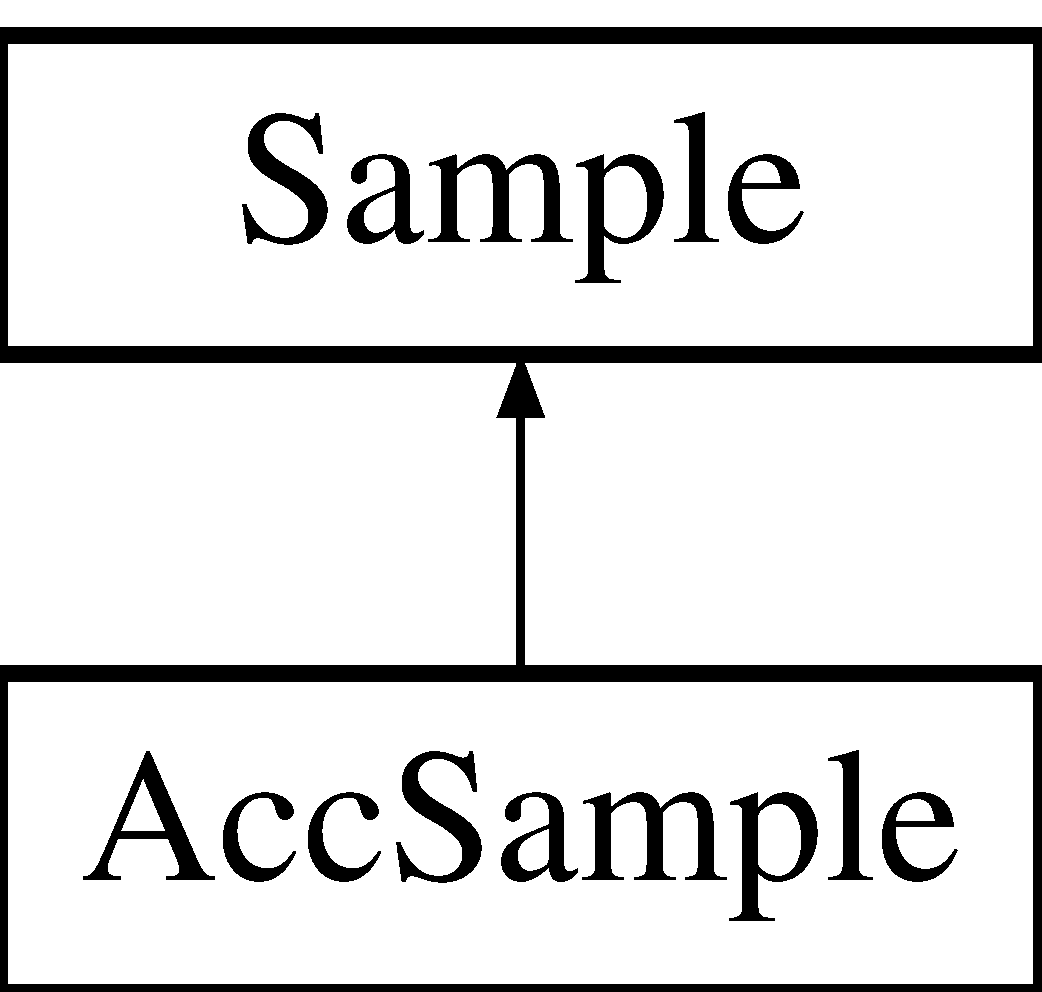
\includegraphics[height=2.000000cm]{class_acc_sample}
\end{center}
\end{figure}
\subsection*{\-Public \-Member \-Functions}
\begin{DoxyCompactItemize}
\item 
\hypertarget{class_acc_sample_a5892e876569215a5b7b50995a6833f6b}{{\bfseries \-Acc\-Sample} (float x, float y, float z)}\label{class_acc_sample_a5892e876569215a5b7b50995a6833f6b}

\item 
\hypertarget{class_acc_sample_aa34cf984b1524c56192c11fe5675cf05}{{\bfseries \-Acc\-Sample} (const string \&line)}\label{class_acc_sample_aa34cf984b1524c56192c11fe5675cf05}

\item 
\hypertarget{class_acc_sample_a825ac53b7fd8d13dfe91c985f07ceb46}{float {\bfseries x} () const }\label{class_acc_sample_a825ac53b7fd8d13dfe91c985f07ceb46}

\item 
\hypertarget{class_acc_sample_a55d458e0aa735db6b64282d080f724ff}{float {\bfseries y} () const }\label{class_acc_sample_a55d458e0aa735db6b64282d080f724ff}

\item 
\hypertarget{class_acc_sample_ab9345c09ebedc152069f1b85c932db55}{float {\bfseries z} () const }\label{class_acc_sample_ab9345c09ebedc152069f1b85c932db55}

\item 
\hypertarget{class_acc_sample_ad505a6ecf1789caa9a49be3f3bbd113b}{virtual void {\bfseries save} (ofstream \&out)}\label{class_acc_sample_ad505a6ecf1789caa9a49be3f3bbd113b}

\item 
\hypertarget{class_sample_ae728243bef5e290d46a2851ea2ce5fe2}{void {\bfseries set\-Log\-Type} (int l)}\label{class_sample_ae728243bef5e290d46a2851ea2ce5fe2}

\item 
\hypertarget{class_sample_aafff0e8223f3eafa001611a63f194c8a}{int {\bfseries get\-Log\-Type} () const }\label{class_sample_aafff0e8223f3eafa001611a63f194c8a}

\item 
\hypertarget{class_sample_a05edd06782fa94517b8daeb29e12057d}{void {\bfseries set\-Timestamp\-From\-Gesture\-Start} (unsigned long t)}\label{class_sample_a05edd06782fa94517b8daeb29e12057d}

\item 
\hypertarget{class_sample_a94a34fe92c0f8a89485042aaea458d94}{unsigned long {\bfseries get\-Timestamp\-From\-Gesture\-Start} () const }\label{class_sample_a94a34fe92c0f8a89485042aaea458d94}

\end{DoxyCompactItemize}
\subsection*{\-Protected \-Attributes}
\begin{DoxyCompactItemize}
\item 
\hypertarget{class_sample_a24ea733ab0a815949a57aca2a4740e33}{unsigned long {\bfseries rel\-Timestamp}}\label{class_sample_a24ea733ab0a815949a57aca2a4740e33}

\item 
\hypertarget{class_sample_a3a6454628c790459f41de5c83bf3ec7c}{int {\bfseries log\-Type}}\label{class_sample_a3a6454628c790459f41de5c83bf3ec7c}

\end{DoxyCompactItemize}
\subsection*{\-Private \-Attributes}
\begin{DoxyCompactItemize}
\item 
\hypertarget{class_acc_sample_a0971152a4b39e44f004fb3d617c0a285}{float {\bfseries ax}}\label{class_acc_sample_a0971152a4b39e44f004fb3d617c0a285}

\item 
\hypertarget{class_acc_sample_a1fd5b59dc902551e02efc4fe2c83695e}{float {\bfseries ay}}\label{class_acc_sample_a1fd5b59dc902551e02efc4fe2c83695e}

\item 
\hypertarget{class_acc_sample_a332097e8c2743fa40a586a50efdb7efe}{float {\bfseries az}}\label{class_acc_sample_a332097e8c2743fa40a586a50efdb7efe}

\end{DoxyCompactItemize}


\subsection{\-Detailed \-Description}


\-Definition at line 6 of file accsample.\-h.



\-The documentation for this class was generated from the following files\-:\begin{DoxyCompactItemize}
\item 
accsample.\-h\item 
accsample.\-cpp\end{DoxyCompactItemize}

\hypertarget{structang3f__t}{\section{ang3f\-\_\-t Struct Reference}
\label{structang3f__t}\index{ang3f\-\_\-t@{ang3f\-\_\-t}}
}


R\-P\-Y float angles.  




{\ttfamily \#include $<$wiic\-\_\-structs.\-h$>$}

\subsection*{Public Attributes}
\begin{DoxyCompactItemize}
\item 
\hypertarget{structang3f__t_ae20d5612a396169a552d5cf1331ff44e}{float {\bfseries roll}}\label{structang3f__t_ae20d5612a396169a552d5cf1331ff44e}

\item 
\hypertarget{structang3f__t_a6b502912c6e6310980794a6659d1bb60}{float {\bfseries pitch}}\label{structang3f__t_a6b502912c6e6310980794a6659d1bb60}

\item 
\hypertarget{structang3f__t_a4aaa40b1ad6ca3477e92a40eab30f18f}{float {\bfseries yaw}}\label{structang3f__t_a4aaa40b1ad6ca3477e92a40eab30f18f}

\item 
\hypertarget{structang3f__t_a09595b789ac278dae9703697713b53a9}{float {\bfseries r}}\label{structang3f__t_a09595b789ac278dae9703697713b53a9}

\item 
\hypertarget{structang3f__t_a009fcdb7a86a7c5e54738dc23fe53443}{float {\bfseries p}}\label{structang3f__t_a009fcdb7a86a7c5e54738dc23fe53443}

\item 
\hypertarget{structang3f__t_a6f9590858061faa6ae701510664937c8}{float {\bfseries y}}\label{structang3f__t_a6f9590858061faa6ae701510664937c8}

\end{DoxyCompactItemize}


\subsection{Detailed Description}
R\-P\-Y float angles. 

Definition at line 99 of file wiic\-\_\-r90/src/wiic/wiic\-\_\-structs.\-h.



The documentation for this struct was generated from the following files\-:\begin{DoxyCompactItemize}
\item 
\hyperlink{wiic__r90_2src_2wiic_2wiic__structs_8h}{wiic\-\_\-r90/src/wiic/wiic\-\_\-structs.\-h}\item 
\hyperlink{wiic__v1_81_2src_2wiic_2wiic__structs_8h}{wiic\-\_\-v1.\-1/src/wiic/wiic\-\_\-structs.\-h}\end{DoxyCompactItemize}

\hypertarget{structang3s__t}{\section{ang3s\-\_\-t \-Struct \-Reference}
\label{structang3s__t}\index{ang3s\-\_\-t@{ang3s\-\_\-t}}
}


\-R\-P\-Y short int angles.  




{\ttfamily \#include $<$wiic\-\_\-structs.\-h$>$}

\subsection*{\-Public \-Attributes}
\begin{DoxyCompactItemize}
\item 
\hypertarget{structang3s__t_a1cacb79df7b3e902fe82e4b8be991675}{short {\bfseries roll}}\label{structang3s__t_a1cacb79df7b3e902fe82e4b8be991675}

\item 
\hypertarget{structang3s__t_a1c649065f433716dd2e995394a1bd21d}{short {\bfseries pitch}}\label{structang3s__t_a1c649065f433716dd2e995394a1bd21d}

\item 
\hypertarget{structang3s__t_ac387b50cc3ff1813fa564d086f985dc7}{short {\bfseries yaw}}\label{structang3s__t_ac387b50cc3ff1813fa564d086f985dc7}

\end{DoxyCompactItemize}


\subsection{\-Detailed \-Description}
\-R\-P\-Y short int angles. 

\-Definition at line 91 of file wiic\-\_\-structs.\-h.



\-The documentation for this struct was generated from the following file\-:\begin{DoxyCompactItemize}
\item 
\hyperlink{wiic__structs_8h}{wiic\-\_\-structs.\-h}\end{DoxyCompactItemize}

\hypertarget{structang__rate__t}{\section{ang\-\_\-rate\-\_\-t \-Struct \-Reference}
\label{structang__rate__t}\index{ang\-\_\-rate\-\_\-t@{ang\-\_\-rate\-\_\-t}}
}


\-Angular rate struct.  




{\ttfamily \#include $<$wiic\-\_\-structs.\-h$>$}

\subsection*{\-Public \-Attributes}
\begin{DoxyCompactItemize}
\item 
\hypertarget{structang__rate__t_aa1fa5093d421095a2eeae1ad07b341eb}{struct \hyperlink{structang3f__t}{ang3f\-\_\-t} \hyperlink{structang__rate__t_aa1fa5093d421095a2eeae1ad07b341eb}{rate}}\label{structang__rate__t_aa1fa5093d421095a2eeae1ad07b341eb}

\begin{DoxyCompactList}\small\item\em roll, pitch and yaw rate (this may be smoothed if enabled) \end{DoxyCompactList}\item 
\hypertarget{structang__rate__t_a255841f280d6b3e0bc07549ccabb9a4c}{struct \hyperlink{structang3f__t}{ang3f\-\_\-t} \hyperlink{structang__rate__t_a255841f280d6b3e0bc07549ccabb9a4c}{a\-\_\-rate}}\label{structang__rate__t_a255841f280d6b3e0bc07549ccabb9a4c}

\begin{DoxyCompactList}\small\item\em roll, pitch and yaw rate (unsmoothed) \end{DoxyCompactList}\end{DoxyCompactItemize}


\subsection{\-Detailed \-Description}
\-Angular rate struct. 

\-Yaw, pitch, and roll rate from -\/180 to 180 degrees. 

\-Definition at line 119 of file wiic\-\_\-structs.\-h.



\-The documentation for this struct was generated from the following file\-:\begin{DoxyCompactItemize}
\item 
\hyperlink{wiic__structs_8h}{wiic\-\_\-structs.\-h}\end{DoxyCompactItemize}

\hypertarget{structbalance__board__t}{\section{balance\-\_\-board\-\_\-t Struct Reference}
\label{structbalance__board__t}\index{balance\-\_\-board\-\_\-t@{balance\-\_\-board\-\_\-t}}
}


Balance Board expansion device.  




{\ttfamily \#include $<$wiic\-\_\-structs.\-h$>$}

\subsection*{Public Attributes}
\begin{DoxyCompactItemize}
\item 
\hypertarget{structbalance__board__t_a0ba9ccde483558b820c8062757864bad}{struct \hyperlink{structpressure__t}{pressure\-\_\-t} {\bfseries cal\-\_\-low\-\_\-weight}}\label{structbalance__board__t_a0ba9ccde483558b820c8062757864bad}

\item 
\hypertarget{structbalance__board__t_a04836ca22dad56206232b1b7836ff023}{struct \hyperlink{structpressure__t}{pressure\-\_\-t} {\bfseries cal\-\_\-medium\-\_\-weight}}\label{structbalance__board__t_a04836ca22dad56206232b1b7836ff023}

\item 
\hypertarget{structbalance__board__t_a9efb8f44640fa6ef0b459322335fad93}{struct \hyperlink{structpressure__t}{pressure\-\_\-t} {\bfseries cal\-\_\-high\-\_\-weight}}\label{structbalance__board__t_a9efb8f44640fa6ef0b459322335fad93}

\item 
\hypertarget{structbalance__board__t_a758120272d9ea7e0257ff8106d746e70}{struct \hyperlink{structpressure__t}{pressure\-\_\-t} {\bfseries pressure\-\_\-raw\-\_\-data}}\label{structbalance__board__t_a758120272d9ea7e0257ff8106d746e70}

\item 
\hypertarget{structbalance__board__t_af1fc954c03bb9c1aec63c57d732c7e0e}{struct \hyperlink{structpressure__weight__t}{pressure\-\_\-weight\-\_\-t} {\bfseries pressure\-\_\-weight}}\label{structbalance__board__t_af1fc954c03bb9c1aec63c57d732c7e0e}

\end{DoxyCompactItemize}


\subsection{Detailed Description}
Balance Board expansion device. 

Definition at line 322 of file wiic\-\_\-structs.\-h.



The documentation for this struct was generated from the following file\-:\begin{DoxyCompactItemize}
\item 
\hyperlink{wiic__structs_8h}{wiic\-\_\-structs.\-h}\end{DoxyCompactItemize}

\hypertarget{class_c_accelerometer}{\section{\-C\-Accelerometer \-Class \-Reference}
\label{class_c_accelerometer}\index{\-C\-Accelerometer@{\-C\-Accelerometer}}
}
\subsection*{\-Public \-Member \-Functions}
\begin{DoxyCompactItemize}
\item 
\hypertarget{class_c_accelerometer_ac6a043c178545a10a47134638ab243df}{{\bfseries \-C\-Accelerometer} (struct \hyperlink{structaccel__t}{accel\-\_\-t} $\ast$\-Accel\-Cal\-Ptr, struct \hyperlink{structvec3b__t}{vec3b\-\_\-t} $\ast$\-Acceleration\-Ptr, int $\ast$\-Accel\-Threshold\-Ptr, struct \hyperlink{structorient__t}{orient\-\_\-t} $\ast$\-Orientation\-Ptr, float $\ast$\-Orientation\-Threshold\-Ptr, struct \hyperlink{structgforce__t}{gforce\-\_\-t} $\ast$\-G\-Force\-Ptr)}\label{class_c_accelerometer_ac6a043c178545a10a47134638ab243df}

\item 
\hypertarget{class_c_accelerometer_a09ce4dcabd897c0231569ebc9f476e6b}{float {\bfseries \-Set\-Smooth\-Alpha} (float \-Alpha)}\label{class_c_accelerometer_a09ce4dcabd897c0231569ebc9f476e6b}

\item 
\hypertarget{class_c_accelerometer_a5d4a662244592cf20751711c298781e5}{float {\bfseries \-Get\-Orient\-Threshold} ()}\label{class_c_accelerometer_a5d4a662244592cf20751711c298781e5}

\item 
\hypertarget{class_c_accelerometer_a4a5f3f55dce8a3a8a049ee38c121e00e}{void {\bfseries \-Set\-Orient\-Threshold} (float \-Threshold)}\label{class_c_accelerometer_a4a5f3f55dce8a3a8a049ee38c121e00e}

\item 
\hypertarget{class_c_accelerometer_a51262cabf03ac689875b6cb37f27f253}{int {\bfseries \-Get\-Accel\-Threshold} ()}\label{class_c_accelerometer_a51262cabf03ac689875b6cb37f27f253}

\item 
\hypertarget{class_c_accelerometer_a8e2e5501d5d151558206eb61f0e24b99}{void {\bfseries \-Set\-Accel\-Threshold} (int \-Threshold)}\label{class_c_accelerometer_a8e2e5501d5d151558206eb61f0e24b99}

\item 
void \hyperlink{class_c_accelerometer_ae332fb3f201d67f554328fadaa343fe0}{\-Get\-Orientation} (float \&\-Pitch, float \&\-Roll, float \&\-Yaw)
\begin{DoxyCompactList}\small\item\em \-Retrieves the smoothed device attitude (pitch, roll, and yaw) computed with an exponential moving average. \end{DoxyCompactList}\item 
\hypertarget{class_c_accelerometer_a8813b02e69b3072f4190b9779954b79d}{void {\bfseries \-Get\-Gravity\-Cal\-Vector} (float \&\-X, float \&\-Y, float \&\-Z)}\label{class_c_accelerometer_a8813b02e69b3072f4190b9779954b79d}

\item 
\hypertarget{class_c_accelerometer_afa6961a116ebc581da421b17b3976e92}{void {\bfseries \-Set\-Gravity\-Cal\-Vector} (float \-X, float \-Y, float \-Z)}\label{class_c_accelerometer_afa6961a116ebc581da421b17b3976e92}

\item 
\hypertarget{class_c_accelerometer_ad2b57ead77ae9d6abe9d28b070e0f891}{void {\bfseries \-Get\-Gravity\-Vector} (float \&\-X, float \&\-Y, float \&\-Z)}\label{class_c_accelerometer_ad2b57ead77ae9d6abe9d28b070e0f891}

\item 
\hypertarget{class_c_accelerometer_af318f42e0e26b5122eb3a1d82919baa4}{void {\bfseries \-Get\-Raw\-Gravity\-Vector} (float \&\-X, float \&\-Y, float \&\-Z)}\label{class_c_accelerometer_af318f42e0e26b5122eb3a1d82919baa4}

\end{DoxyCompactItemize}
\subsection*{\-Private \-Attributes}
\begin{DoxyCompactItemize}
\item 
\hypertarget{class_c_accelerometer_a121c813be993f72ad2563fd27f3857a7}{struct \hyperlink{structaccel__t}{accel\-\_\-t} $\ast$ {\bfseries mp\-Accel\-Calib\-Ptr}}\label{class_c_accelerometer_a121c813be993f72ad2563fd27f3857a7}

\item 
\hypertarget{class_c_accelerometer_a9d98ce13ae72eea33a80548a384de565}{struct \hyperlink{structvec3b__t}{vec3b\-\_\-t} $\ast$ {\bfseries mp\-Accel\-Ptr}}\label{class_c_accelerometer_a9d98ce13ae72eea33a80548a384de565}

\item 
\hypertarget{class_c_accelerometer_a9d3e8f3e481f9d1f12e52de03b4dba52}{struct \hyperlink{structorient__t}{orient\-\_\-t} $\ast$ {\bfseries mp\-Orient\-Ptr}}\label{class_c_accelerometer_a9d3e8f3e481f9d1f12e52de03b4dba52}

\item 
\hypertarget{class_c_accelerometer_adeb9c7760b24329e98f6991b934c7237}{struct \hyperlink{structgforce__t}{gforce\-\_\-t} $\ast$ {\bfseries mp\-G\-Force\-Ptr}}\label{class_c_accelerometer_adeb9c7760b24329e98f6991b934c7237}

\item 
\hypertarget{class_c_accelerometer_abc3dac2cc1659a873d328d8f50cd3985}{int $\ast$ {\bfseries mp\-Accel\-Threshold\-Ptr}}\label{class_c_accelerometer_abc3dac2cc1659a873d328d8f50cd3985}

\item 
\hypertarget{class_c_accelerometer_a10e1ee61f93ece8b81f231ddf4898c23}{float $\ast$ {\bfseries mp\-Orient\-Threshold\-Ptr}}\label{class_c_accelerometer_a10e1ee61f93ece8b81f231ddf4898c23}

\end{DoxyCompactItemize}


\subsection{\-Detailed \-Description}


\-Definition at line 166 of file wiicpp.\-h.



\subsection{\-Member \-Function \-Documentation}
\hypertarget{class_c_accelerometer_ae332fb3f201d67f554328fadaa343fe0}{\index{\-C\-Accelerometer@{\-C\-Accelerometer}!\-Get\-Orientation@{\-Get\-Orientation}}
\index{\-Get\-Orientation@{\-Get\-Orientation}!CAccelerometer@{\-C\-Accelerometer}}
\subsubsection[{\-Get\-Orientation}]{\setlength{\rightskip}{0pt plus 5cm}void {\bf \-C\-Accelerometer\-::\-Get\-Orientation} (
\begin{DoxyParamCaption}
\item[{float \&}]{\-Pitch, }
\item[{float \&}]{\-Roll, }
\item[{float \&}]{\-Yaw}
\end{DoxyParamCaption}
)}}\label{class_c_accelerometer_ae332fb3f201d67f554328fadaa343fe0}


\-Retrieves the smoothed device attitude (pitch, roll, and yaw) computed with an exponential moving average. 


\begin{DoxyParams}{\-Parameters}
{\em \-Pitch} & \mbox{[}out\mbox{]} \-Reference variable where the smooth device pitch will be set. \\
\hline
{\em \-Roll} & \mbox{[}out\mbox{]} \-Reference variable where the smooth device roll will be set. \\
\hline
{\em \-Yaw} & \mbox{[}out\mbox{]} \-Reference variable where the smooth device yaw will be set. \-Please, note that without \-I\-R enabled, yaw cannot be retrieved. \\
\hline
\end{DoxyParams}


\-Definition at line 205 of file wiicpp.\-cpp.



\-The documentation for this class was generated from the following files\-:\begin{DoxyCompactItemize}
\item 
wiicpp.\-h\item 
wiicpp.\-cpp\end{DoxyCompactItemize}

\hypertarget{class_camera}{\section{Camera Class Reference}
\label{class_camera}\index{Camera@{Camera}}
}


The \hyperlink{class_camera}{Camera} class represents a logical camera in a model view, which posesses a current viewing angle and an absolute position in space as its state.  




{\ttfamily \#include $<$Camera.\-hpp$>$}

\subsection*{Public Types}
\begin{DoxyCompactItemize}
\item 
enum \hyperlink{class_camera_a80cb65605322d27ad3b6d973484509ec}{Direction} \{ \\*
{\bfseries Forward}, 
{\bfseries Backward}, 
{\bfseries Left}, 
{\bfseries Right}, 
\\*
{\bfseries Up}, 
{\bfseries Down}, 
{\bfseries End}, 
{\bfseries Begin} =  Forward
 \}
\begin{DoxyCompactList}\small\item\em The Direction enumeration lists all of the possible directions the camera may travel in. \end{DoxyCompactList}\item 
enum \hyperlink{class_camera_a6ff726a75a430e4f17e5dec42e4d4405}{glsl\-\_\-var} \{ \\*
{\bfseries T\-R\-A\-N\-S\-L\-A\-T\-I\-O\-N}, 
{\bfseries R\-O\-T\-A\-T\-I\-O\-N}, 
{\bfseries V\-I\-E\-W}, 
{\bfseries C\-T\-M}, 
\\*
{\bfseries Num\-Glsl\-Vars}
 \}
\begin{DoxyCompactList}\small\item\em The glsl\-\_\-var enumeration lists the various variables the \hyperlink{class_camera}{Camera} class is capable of sending to the shader. \end{DoxyCompactList}\item 
enum \hyperlink{class_camera_afdccec6d447490dcc80ab6b99f21d0e5}{view\-\_\-type} \{ \\*
{\bfseries P\-E\-R\-S\-P\-E\-C\-T\-I\-V\-E}, 
{\bfseries O\-R\-T\-H\-O}, 
{\bfseries O\-R\-T\-H\-O2\-D}, 
{\bfseries I\-D\-E\-N\-T\-I\-T\-Y}, 
\\*
{\bfseries F\-R\-U\-S\-T\-U\-M}
 \}
\begin{DoxyCompactList}\small\item\em The view\-\_\-type enumeration lists the various possibilities for the current viewing mode that can be switched between. \end{DoxyCompactList}\end{DoxyCompactItemize}
\subsection*{Public Member Functions}
\begin{DoxyCompactItemize}
\item 
\hyperlink{class_camera_a47104bf17f448c97bf7bb34360ab8fcc}{Camera} (float x=0.\-0, float y=0.\-0, float z=0.\-0)
\begin{DoxyCompactList}\small\item\em Initialization Constructor; sets the X,Y,Z coordinates explicitly. \end{DoxyCompactList}\item 
\hyperlink{class_camera_a388c39247312dc6850b2d1b007efb423}{Camera} (\hyperlink{struct_angel_1_1vec3}{vec3} \&in)
\begin{DoxyCompactList}\small\item\em Initialization Constructor, uses a vec3 as its initial coordinates. \end{DoxyCompactList}\item 
\hyperlink{class_camera_a30b637b0e81821106c16a8a299d24d3f}{Camera} (\hyperlink{struct_angel_1_1vec4}{vec4} \&in)
\begin{DoxyCompactList}\small\item\em Initialization Constructor, uses a vec4 as its initial coordinates. \end{DoxyCompactList}\item 
virtual \hyperlink{class_camera_a06211f202c145b3ec8253f96e1e654a6}{$\sim$\-Camera} (void)
\begin{DoxyCompactList}\small\item\em Default destructor. \end{DoxyCompactList}\item 
void \hyperlink{class_camera_a7ff7cf14bee873ac6cda7b2e42a60358}{X} (const float \&in, const bool \&update=true)
\begin{DoxyCompactList}\small\item\em Sets the X coordinate of the camera. \end{DoxyCompactList}\item 
void \hyperlink{class_camera_a69af560bb7f85db3a5062d1a6b3927bf}{Y} (const float \&in, const bool \&update=true)
\begin{DoxyCompactList}\small\item\em Sets the Y coordinate of the camera. \end{DoxyCompactList}\item 
void \hyperlink{class_camera_a38438f8e2417a3a40eaad85d2ab344a9}{Z} (const float \&in, const bool \&update=true)
\begin{DoxyCompactList}\small\item\em Sets the Z coordinate of the camera. \end{DoxyCompactList}\item 
void \hyperlink{class_camera_a432e03c15d63f8839fe4731016d907a4}{pos} (const float \&x, const float \&y, const float \&z, const bool \&update=true)
\begin{DoxyCompactList}\small\item\em Sets the absolute position of the camera. \end{DoxyCompactList}\item 
void \hyperlink{class_camera_ae9dc2206b71b25cf320a05d148cb8b56}{pos} (const \hyperlink{struct_angel_1_1vec3}{vec3} \&in, const bool \&update=true)
\begin{DoxyCompactList}\small\item\em Sets the absolute position of the camera. \end{DoxyCompactList}\item 
void \hyperlink{class_camera_aec2115038562e514193bb2b67f5da153}{pos} (const \hyperlink{struct_angel_1_1vec4}{vec4} \&in, const bool \&update=true)
\begin{DoxyCompactList}\small\item\em Sets the absolute position of the camera. \end{DoxyCompactList}\item 
void \hyperlink{class_camera_ac7985a6cb48f4e1e74fda17e5213dd74}{d\-X} (const float \&by, const bool \&update=true)
\begin{DoxyCompactList}\small\item\em Moves the camera along the X axis. \end{DoxyCompactList}\item 
void \hyperlink{class_camera_a59570a88e3ff2d277c9e995372fcadfe}{d\-Y} (const float \&by, const bool \&update=true)
\begin{DoxyCompactList}\small\item\em Moves the camera along the Y axis. \end{DoxyCompactList}\item 
void \hyperlink{class_camera_ab94ed9b3c7e12f484d6bfa5f827b59ff}{d\-Z} (const float \&by, const bool \&update=true)
\begin{DoxyCompactList}\small\item\em Moves the camera along the Z axis. \end{DoxyCompactList}\item 
void \hyperlink{class_camera_a2ac5f89b4f9f012dead66980925143c0}{d\-Pos} (const float \&x, const float \&y, const float \&z)
\begin{DoxyCompactList}\small\item\em Moves the camera along the x, y, and z axes. \end{DoxyCompactList}\item 
void \hyperlink{class_camera_a928de59670f0b31264307a8a0888b99d}{d\-Pos} (const \hyperlink{struct_angel_1_1vec3}{vec3} \&by)
\begin{DoxyCompactList}\small\item\em Moves the camera along the x, y, and z axes. \end{DoxyCompactList}\item 
void \hyperlink{class_camera_a4ec2e3d2a66826aedb1ac1eee7da0b96}{d\-Pos} (const \hyperlink{struct_angel_1_1vec4}{vec4} \&by)
\begin{DoxyCompactList}\small\item\em Moves the camera along the x, y, and z axes. \end{DoxyCompactList}\item 
void \hyperlink{class_camera_ac325bf616014d2e6023b84b6224630ac}{F\-O\-V} (const float \&\hyperlink{class_camera_acc8b97facc57059530efad534c2f8314}{fovy})
\begin{DoxyCompactList}\small\item\em F\-O\-V sets the current camera Field-\/of-\/view angle. \end{DoxyCompactList}\item 
float \hyperlink{class_camera_a8817ea073431268d8c0e522cdc30026c}{F\-O\-V} (void) const 
\begin{DoxyCompactList}\small\item\em \hyperlink{class_camera_a8817ea073431268d8c0e522cdc30026c}{F\-O\-V()} gets the current camera Field-\/of-\/view angle. \end{DoxyCompactList}\item 
void \hyperlink{class_camera_a55355b3376d195b17adcc6a5b72ae07b}{d\-F\-O\-V} (const float \&by)
\begin{DoxyCompactList}\small\item\em d\-F\-O\-V adjusts the field of view angle up or down by an amount. \end{DoxyCompactList}\item 
void \hyperlink{class_camera_aaadaebb40dc7262abc3f4bc52bc5bfb3}{change\-Perspective} (const \hyperlink{class_camera_afdccec6d447490dcc80ab6b99f21d0e5}{view\-\_\-type} \&v\-Type)
\begin{DoxyCompactList}\small\item\em change\-Perspective changes the current perspective of the camera. \end{DoxyCompactList}\item 
void \hyperlink{class_camera_a24c5346fc0dfaa93257b6716fe0f2421}{refresh\-Perspective} (void)
\begin{DoxyCompactList}\small\item\em refresh\-Perspective re-\/generates the current view/perspective matrix of the camera. \end{DoxyCompactList}\item 
void \hyperlink{class_camera_adda458a9212825164b52019597f2e9c8}{viewport} (size\-\_\-t \-\_\-\-X, size\-\_\-t \-\_\-\-Y, size\-\_\-t \-\_\-width, size\-\_\-t \-\_\-height)
\begin{DoxyCompactList}\small\item\em viewport instructs this camera what his expected drawing window will be. \end{DoxyCompactList}\item 
void \hyperlink{class_camera_abbe6fe82ed05e64e35b0c4ed2001b34e}{sway} (const float \&by)
\begin{DoxyCompactList}\small\item\em Adjusts the camera's X coordinate relative to its current position. \end{DoxyCompactList}\item 
void \hyperlink{class_camera_abb2251df65445bf8efd3fe0074fb5033}{surge} (const float \&by)
\begin{DoxyCompactList}\small\item\em Adjusts the camera's Z coordinate relative to its current position. \end{DoxyCompactList}\item 
void \hyperlink{class_camera_a2148d751f104d8e39c9832e2372df2d9}{heave} (const float \&by)
\begin{DoxyCompactList}\small\item\em Adjusts the camera's Y coordinate relative to its current position. \end{DoxyCompactList}\item 
void \hyperlink{class_camera_aac7dbb6201be7f17e014fc6fdf915560}{pitch} (const float \&by, const bool \&fixed=false)
\begin{DoxyCompactList}\small\item\em pitch adjusts the X axis rotation; up/down look. \end{DoxyCompactList}\item 
void \hyperlink{class_camera_a0ce7d12edbe47d9a8915d8af98d8f524}{yaw} (const float \&by, const bool \&fixed=false)
\begin{DoxyCompactList}\small\item\em yaw adjusts the Y axis rotation; left/right look. \end{DoxyCompactList}\item 
void \hyperlink{class_camera_a1ba0979fe0b2ec58085d5f9721858e5e}{roll} (const float \&by, const bool \&fixed=false)
\begin{DoxyCompactList}\small\item\em roll adjusts the Z axis rotation; tilt or lean left/right. \end{DoxyCompactList}\item 
void \hyperlink{class_camera_a421e03f93824e178d6e77ff547cd290e}{Move} (const \hyperlink{class_camera_a80cb65605322d27ad3b6d973484509ec}{Camera\-::\-Direction} \&Dir)
\begin{DoxyCompactList}\small\item\em Move instructs the camera to begin moving in the specified direction. \end{DoxyCompactList}\item 
void \hyperlink{class_camera_adf064f765f610684e0675bd67de013fd}{Stop} (const \hyperlink{class_camera_a80cb65605322d27ad3b6d973484509ec}{Camera\-::\-Direction} \&Dir)
\begin{DoxyCompactList}\small\item\em Stop instructs the camera to stop moving in the specified direction. \end{DoxyCompactList}\item 
void \hyperlink{class_camera_aec3559fe43597656629fdb00157d3c73}{Idle} (void)
\begin{DoxyCompactList}\small\item\em Idle moves the camera forward in whichever directions it is configured to move in. \end{DoxyCompactList}\item 
void \hyperlink{class_camera_a8eb4ebda2379e7289bb2bb942a2796b4}{Accel} (const \hyperlink{struct_angel_1_1vec3}{vec3} \&accel)
\begin{DoxyCompactList}\small\item\em Accel takes an input vec2 which represents an acceleration, and applies it to the motion vectors with regards to the maximum acceleration and the maximum speed of the camera. \end{DoxyCompactList}\item 
float \hyperlink{class_camera_a2f7fd64d5d6e0dfb5edcca53c7d15994}{X} (void) const 
\begin{DoxyCompactList}\small\item\em \hyperlink{class_camera_a2f7fd64d5d6e0dfb5edcca53c7d15994}{X()} returns the current position of the camera in model coordinates. \end{DoxyCompactList}\item 
float \hyperlink{class_camera_a37529ef93871f547ebfd5862bc6cce62}{Y} (void) const 
\begin{DoxyCompactList}\small\item\em \hyperlink{class_camera_a37529ef93871f547ebfd5862bc6cce62}{Y()} returns the current position of the camera in model coordinates. \end{DoxyCompactList}\item 
float \hyperlink{class_camera_abf1730e47e8e51c76acbddcaa85e2475}{Z} (void) const 
\begin{DoxyCompactList}\small\item\em \hyperlink{class_camera_abf1730e47e8e51c76acbddcaa85e2475}{Z()} returns the current position of the camera in model coordinates. \end{DoxyCompactList}\item 
\hyperlink{struct_angel_1_1vec4}{vec4} \hyperlink{class_camera_a9982ac5f48fe0af97fefa725080d6da6}{pos} (void) const 
\begin{DoxyCompactList}\small\item\em \hyperlink{class_camera_a9982ac5f48fe0af97fefa725080d6da6}{pos()} gets the current camera position in model coordinates. \end{DoxyCompactList}\item 
void \hyperlink{class_camera_a36cba68c08136242bf5d906f9c0b610c}{send} (const \hyperlink{class_camera_a6ff726a75a430e4f17e5dec42e4d4405}{glsl\-\_\-var} \&which)
\begin{DoxyCompactList}\small\item\em send will send a glsl variable to the shader. \end{DoxyCompactList}\item 
void \hyperlink{class_camera_ad02f12a279c33e7e85dcaf88830d38c7}{link} (const G\-Luint \&program, const \hyperlink{class_camera_a6ff726a75a430e4f17e5dec42e4d4405}{glsl\-\_\-var} \&which, const string \&glsl\-Var\-Name)
\begin{DoxyCompactList}\small\item\em Link associates the camera with a glsl uniform variable. \end{DoxyCompactList}\item 
void \hyperlink{class_camera_a9d96971546c610e534f603a0f41e32b2}{Draw} (void)
\begin{DoxyCompactList}\small\item\em Draw will instruct Open\-G\-L of the viewport we want, and then send all of our current matrices to the shader for rendering. \end{DoxyCompactList}\end{DoxyCompactItemize}
\subsection*{Private Member Functions}
\begin{DoxyCompactItemize}
\item 
void \hyperlink{class_camera_aba32f195cdb5bfcfd05c2ce74315b6c3}{adjust\-Rotation} (const \hyperlink{class_angel_1_1mat4}{mat4} \&adjustment, const bool \&fixed=false)
\begin{DoxyCompactList}\small\item\em adjust\-Rotation is an internal function that rotates the camera. \end{DoxyCompactList}\item 
void \hyperlink{class_camera_a20243a7e3eb06ab1265118c5fb9cce9b}{common\-Init} (void)
\begin{DoxyCompactList}\small\item\em commin\-Init is a private function that initializes local object attributes. \end{DoxyCompactList}\end{DoxyCompactItemize}
\subsection*{Private Attributes}
\begin{DoxyCompactItemize}
\item 
\hyperlink{class_angel_1_1mat4}{mat4} \hyperlink{class_camera_aa4cb92b539c9a9707a12d7025ed889f6}{T}
\begin{DoxyCompactList}\small\item\em The current translation matrix for this camera. \end{DoxyCompactList}\item 
\hyperlink{class_angel_1_1mat4}{mat4} \hyperlink{class_camera_a8fd028120b18556c43ad86756e637fbc}{R}
\begin{DoxyCompactList}\small\item\em The current rotational matrix for this camera. \end{DoxyCompactList}\item 
\hyperlink{class_angel_1_1mat4}{mat4} \hyperlink{class_camera_a0bee6fbae6ec5960850a5fb858f3912a}{P}
\begin{DoxyCompactList}\small\item\em The current view matrix (usually perspective) for this camera. \end{DoxyCompactList}\item 
\hyperlink{class_angel_1_1mat4}{mat4} \hyperlink{class_camera_a9b1e81e3f5531390bb6a599dca0d2444}{ctm}
\begin{DoxyCompactList}\small\item\em The 'Current Transformation Matrix' for this camera. \end{DoxyCompactList}\item 
\hyperlink{class_camera_afdccec6d447490dcc80ab6b99f21d0e5}{view\-\_\-type} \hyperlink{class_camera_a1fe2ef68d26bb98f0aa736948304eb64}{curr\-View}
\begin{DoxyCompactList}\small\item\em The current viewing mode type. \end{DoxyCompactList}\item 
G\-Lfloat \hyperlink{class_camera_a308e92b5d3ef0eea5cac7745df6e28f4}{speed}
\begin{DoxyCompactList}\small\item\em Current Speed of camera motion. \end{DoxyCompactList}\item 
\hyperlink{struct_angel_1_1vec3}{vec3} \hyperlink{class_camera_a5b95c890f213db50f321380108b17ea1}{velocity}
\begin{DoxyCompactList}\small\item\em Current Velocity of camera motion. \end{DoxyCompactList}\item 
\hypertarget{class_camera_aa075ae6872228fc4db892533d9f6d881}{G\-Lfloat \hyperlink{class_camera_aa075ae6872228fc4db892533d9f6d881}{speed\-\_\-cap}}\label{class_camera_aa075ae6872228fc4db892533d9f6d881}

\begin{DoxyCompactList}\small\item\em Current Speed Capacity\-: (speed/\-Max\-Speed) \end{DoxyCompactList}\item 
\hypertarget{class_camera_a7817b2e83ad8f783e2822ec7771c6fe9}{G\-Lfloat \hyperlink{class_camera_a7817b2e83ad8f783e2822ec7771c6fe9}{Max\-Accel}}\label{class_camera_a7817b2e83ad8f783e2822ec7771c6fe9}

\begin{DoxyCompactList}\small\item\em Maximum Acceleration Magnitude. \end{DoxyCompactList}\item 
\hypertarget{class_camera_a4e6866298a8e7a1ff2f529202892958e}{G\-Lfloat \hyperlink{class_camera_a4e6866298a8e7a1ff2f529202892958e}{Max\-Speed}}\label{class_camera_a4e6866298a8e7a1ff2f529202892958e}

\begin{DoxyCompactList}\small\item\em Maximum Speed. \end{DoxyCompactList}\item 
G\-Lfloat \hyperlink{class_camera_a4260507a4e59b2b079a0e1c6a5b64d5c}{Friction\-Magnitude}
\begin{DoxyCompactList}\small\item\em Friction. \end{DoxyCompactList}\item 
G\-Lfloat \hyperlink{class_camera_af3fdbc52ba0f7af7d8091986d6303119}{aspect}
\begin{DoxyCompactList}\small\item\em Current aspect ratio for certain perspectives. \end{DoxyCompactList}\item 
G\-Lfloat \hyperlink{class_camera_acc8b97facc57059530efad534c2f8314}{fovy}
\begin{DoxyCompactList}\small\item\em Current field-\/of-\/view angle for perspective view. \end{DoxyCompactList}\item 
\hypertarget{class_camera_ad49d7cc9d3e2f90332702cf67f1d5357}{size\-\_\-t \hyperlink{class_camera_ad49d7cc9d3e2f90332702cf67f1d5357}{width}}\label{class_camera_ad49d7cc9d3e2f90332702cf67f1d5357}

\begin{DoxyCompactList}\small\item\em \hyperlink{class_camera}{Camera}'s drawbox width, used for computing (some) perspectives. \end{DoxyCompactList}\item 
\hypertarget{class_camera_a99ad71730dc8fb068b814ca6328e40fa}{size\-\_\-t \hyperlink{class_camera_a99ad71730dc8fb068b814ca6328e40fa}{height}}\label{class_camera_a99ad71730dc8fb068b814ca6328e40fa}

\begin{DoxyCompactList}\small\item\em \hyperlink{class_camera}{Camera}'s drawbox height, used for computing (some) perspectives. \end{DoxyCompactList}\item 
\hypertarget{class_camera_a2e2fc28fcaa8222ac635a568950e6af3}{size\-\_\-t \hyperlink{class_camera_a2e2fc28fcaa8222ac635a568950e6af3}{X\-Pos}}\label{class_camera_a2e2fc28fcaa8222ac635a568950e6af3}

\begin{DoxyCompactList}\small\item\em \hyperlink{class_camera}{Camera}'s Viewport's X-\/\-Position Offset. \end{DoxyCompactList}\item 
\hypertarget{class_camera_af15974390620818974704b6e88cfedbd}{size\-\_\-t \hyperlink{class_camera_af15974390620818974704b6e88cfedbd}{Y\-Pos}}\label{class_camera_af15974390620818974704b6e88cfedbd}

\begin{DoxyCompactList}\small\item\em \hyperlink{class_camera}{Camera}'s Viewport's Y-\/\-Position Offset. \end{DoxyCompactList}\item 
bool \hyperlink{class_camera_a39746b4fadf30bba6bdc8aa6acfdc6f2}{Motion} \mbox{[}Camera\-::\-End\mbox{]}
\begin{DoxyCompactList}\small\item\em Booleans correlating to the different motion directions. \end{DoxyCompactList}\item 
G\-Luint \hyperlink{class_camera_a1635486d7f9e0d52b241899a270ee335}{glsl\-\_\-handles} \mbox{[}Camera\-::\-Num\-Glsl\-Vars\mbox{]}
\begin{DoxyCompactList}\small\item\em Handles for communicating with the shader. \end{DoxyCompactList}\end{DoxyCompactItemize}


\subsection{Detailed Description}
The \hyperlink{class_camera}{Camera} class represents a logical camera in a model view, which posesses a current viewing angle and an absolute position in space as its state. 

\begin{DoxyAuthor}{Author}
John Huston, \href{mailto:jhuston@cs.uml.edu}{\tt jhuston@cs.\-uml.\-edu} 
\end{DoxyAuthor}
\begin{DoxySince}{Since}
16 Nov 2012
\end{DoxySince}
Functions are provided to adjust the rotation according to \hyperlink{class_camera_aac7dbb6201be7f17e014fc6fdf915560}{pitch()}, \hyperlink{class_camera_a0ce7d12edbe47d9a8915d8af98d8f524}{yaw()} and \hyperlink{class_camera_a1ba0979fe0b2ec58085d5f9721858e5e}{roll()} motions; \hyperlink{class_camera_abb2251df65445bf8efd3fe0074fb5033}{surge()}, \hyperlink{class_camera_abbe6fe82ed05e64e35b0c4ed2001b34e}{sway()}, and \hyperlink{class_camera_a2148d751f104d8e39c9832e2372df2d9}{heave()} are provided to adjust position in space.

\hyperlink{class_camera_a421e03f93824e178d6e77ff547cd290e}{Move()}, \hyperlink{class_camera_adf064f765f610684e0675bd67de013fd}{Stop()}, and \hyperlink{class_camera_aec3559fe43597656629fdb00157d3c73}{Idle()} are provided to help the camera automatically move along the X, Y, or Z axes. 

Definition at line 30 of file Camera.\-hpp.



\subsection{Member Enumeration Documentation}
\hypertarget{class_camera_a80cb65605322d27ad3b6d973484509ec}{\index{Camera@{Camera}!Direction@{Direction}}
\index{Direction@{Direction}!Camera@{Camera}}
\subsubsection[{Direction}]{\setlength{\rightskip}{0pt plus 5cm}enum {\bf Camera\-::\-Direction}}}\label{class_camera_a80cb65605322d27ad3b6d973484509ec}


The Direction enumeration lists all of the possible directions the camera may travel in. 

'Begin' and 'End' are special sentinel directions for the purposes of iteration, and are ignored by any functions that accept a Direction. 

Definition at line 40 of file Camera.\-hpp.

\hypertarget{class_camera_a6ff726a75a430e4f17e5dec42e4d4405}{\index{Camera@{Camera}!glsl\-\_\-var@{glsl\-\_\-var}}
\index{glsl\-\_\-var@{glsl\-\_\-var}!Camera@{Camera}}
\subsubsection[{glsl\-\_\-var}]{\setlength{\rightskip}{0pt plus 5cm}enum {\bf Camera\-::glsl\-\_\-var}}}\label{class_camera_a6ff726a75a430e4f17e5dec42e4d4405}


The glsl\-\_\-var enumeration lists the various variables the \hyperlink{class_camera}{Camera} class is capable of sending to the shader. 

The Num\-Glsl\-Vars variable is a sentinel value that is ignored by any functions that accept a glsl\-\_\-var. 

Definition at line 58 of file Camera.\-hpp.

\hypertarget{class_camera_afdccec6d447490dcc80ab6b99f21d0e5}{\index{Camera@{Camera}!view\-\_\-type@{view\-\_\-type}}
\index{view\-\_\-type@{view\-\_\-type}!Camera@{Camera}}
\subsubsection[{view\-\_\-type}]{\setlength{\rightskip}{0pt plus 5cm}enum {\bf Camera\-::view\-\_\-type}}}\label{class_camera_afdccec6d447490dcc80ab6b99f21d0e5}


The view\-\_\-type enumeration lists the various possibilities for the current viewing mode that can be switched between. 

The default is P\-E\-R\-S\-P\-E\-C\-T\-I\-V\-E. 

Definition at line 71 of file Camera.\-hpp.



\subsection{Constructor \& Destructor Documentation}
\hypertarget{class_camera_a47104bf17f448c97bf7bb34360ab8fcc}{\index{Camera@{Camera}!Camera@{Camera}}
\index{Camera@{Camera}!Camera@{Camera}}
\subsubsection[{Camera}]{\setlength{\rightskip}{0pt plus 5cm}Camera\-::\-Camera (
\begin{DoxyParamCaption}
\item[{float}]{x = {\ttfamily 0.0}, }
\item[{float}]{y = {\ttfamily 0.0}, }
\item[{float}]{z = {\ttfamily 0.0}}
\end{DoxyParamCaption}
)}}\label{class_camera_a47104bf17f448c97bf7bb34360ab8fcc}


Initialization Constructor; sets the X,Y,Z coordinates explicitly. 


\begin{DoxyParams}{Parameters}
{\em x} & The initial X coordinate. \\
\hline
{\em y} & The initial Y coordinate. \\
\hline
{\em z} & The initial Z coordinate. \\
\hline
\end{DoxyParams}


Definition at line 56 of file Camera.\-cpp.

\hypertarget{class_camera_a388c39247312dc6850b2d1b007efb423}{\index{Camera@{Camera}!Camera@{Camera}}
\index{Camera@{Camera}!Camera@{Camera}}
\subsubsection[{Camera}]{\setlength{\rightskip}{0pt plus 5cm}Camera\-::\-Camera (
\begin{DoxyParamCaption}
\item[{{\bf vec3} \&}]{in}
\end{DoxyParamCaption}
)}}\label{class_camera_a388c39247312dc6850b2d1b007efb423}


Initialization Constructor, uses a vec3 as its initial coordinates. 


\begin{DoxyParams}{Parameters}
{\em in} & A vec3 representing the initial coordinates. \\
\hline
\end{DoxyParams}


Definition at line 67 of file Camera.\-cpp.

\hypertarget{class_camera_a30b637b0e81821106c16a8a299d24d3f}{\index{Camera@{Camera}!Camera@{Camera}}
\index{Camera@{Camera}!Camera@{Camera}}
\subsubsection[{Camera}]{\setlength{\rightskip}{0pt plus 5cm}Camera\-::\-Camera (
\begin{DoxyParamCaption}
\item[{{\bf vec4} \&}]{in}
\end{DoxyParamCaption}
)}}\label{class_camera_a30b637b0e81821106c16a8a299d24d3f}


Initialization Constructor, uses a vec4 as its initial coordinates. 


\begin{DoxyParams}{Parameters}
{\em in} & A vec4 representing the initial coordinates. The w component is ignored. \\
\hline
\end{DoxyParams}


Definition at line 77 of file Camera.\-cpp.

\hypertarget{class_camera_a06211f202c145b3ec8253f96e1e654a6}{\index{Camera@{Camera}!$\sim$\-Camera@{$\sim$\-Camera}}
\index{$\sim$\-Camera@{$\sim$\-Camera}!Camera@{Camera}}
\subsubsection[{$\sim$\-Camera}]{\setlength{\rightskip}{0pt plus 5cm}Camera\-::$\sim$\-Camera (
\begin{DoxyParamCaption}
\item[{void}]{}
\end{DoxyParamCaption}
)\hspace{0.3cm}{\ttfamily [virtual]}}}\label{class_camera_a06211f202c145b3ec8253f96e1e654a6}


Default destructor. 

Nothing of note. 

Definition at line 86 of file Camera.\-cpp.



\subsection{Member Function Documentation}
\hypertarget{class_camera_a8eb4ebda2379e7289bb2bb942a2796b4}{\index{Camera@{Camera}!Accel@{Accel}}
\index{Accel@{Accel}!Camera@{Camera}}
\subsubsection[{Accel}]{\setlength{\rightskip}{0pt plus 5cm}void Camera\-::\-Accel (
\begin{DoxyParamCaption}
\item[{const {\bf vec3} \&}]{raw\-\_\-accel}
\end{DoxyParamCaption}
)}}\label{class_camera_a8eb4ebda2379e7289bb2bb942a2796b4}


Accel takes an input vec2 which represents an acceleration, and applies it to the motion vectors with regards to the maximum acceleration and the maximum speed of the camera. 


\begin{DoxyParams}{Parameters}
{\em raw\-\_\-accel} & The vec3 which represents the (x,y,z) acceleration, where x,y,z are \mbox{[}-\/1,1\mbox{]}. \\
\hline
\end{DoxyParams}
\begin{DoxyReturn}{Returns}
Void. 
\end{DoxyReturn}


Definition at line 374 of file Camera.\-cpp.

\hypertarget{class_camera_aba32f195cdb5bfcfd05c2ce74315b6c3}{\index{Camera@{Camera}!adjust\-Rotation@{adjust\-Rotation}}
\index{adjust\-Rotation@{adjust\-Rotation}!Camera@{Camera}}
\subsubsection[{adjust\-Rotation}]{\setlength{\rightskip}{0pt plus 5cm}void Camera\-::adjust\-Rotation (
\begin{DoxyParamCaption}
\item[{const {\bf mat4} \&}]{adjustment, }
\item[{const bool \&}]{fixed = {\ttfamily false}}
\end{DoxyParamCaption}
)\hspace{0.3cm}{\ttfamily [private]}}}\label{class_camera_aba32f195cdb5bfcfd05c2ce74315b6c3}


adjust\-Rotation is an internal function that rotates the camera. 

Technically, any transformation, not just a rotation, is possible. 
\begin{DoxyParams}{Parameters}
{\em adjustment} & The 4x4 matrix to transform the C\-T\-M by. \\
\hline
{\em fixed} & Should this rotation be fixed about the origin? \\
\hline
\end{DoxyParams}
\begin{DoxyReturn}{Returns}
Void. 
\end{DoxyReturn}


Definition at line 243 of file Camera.\-cpp.

\hypertarget{class_camera_aaadaebb40dc7262abc3f4bc52bc5bfb3}{\index{Camera@{Camera}!change\-Perspective@{change\-Perspective}}
\index{change\-Perspective@{change\-Perspective}!Camera@{Camera}}
\subsubsection[{change\-Perspective}]{\setlength{\rightskip}{0pt plus 5cm}void Camera\-::change\-Perspective (
\begin{DoxyParamCaption}
\item[{const {\bf view\-\_\-type} \&}]{v\-Type}
\end{DoxyParamCaption}
)}}\label{class_camera_aaadaebb40dc7262abc3f4bc52bc5bfb3}


change\-Perspective changes the current perspective of the camera. 


\begin{DoxyParams}{Parameters}
{\em v\-Type} & Which perspective to use. see enum view\-\_\-type for possibilities. \\
\hline
\end{DoxyParams}
\begin{DoxyReturn}{Returns}
Void. 
\end{DoxyReturn}


Definition at line 528 of file Camera.\-cpp.

\hypertarget{class_camera_a20243a7e3eb06ab1265118c5fb9cce9b}{\index{Camera@{Camera}!common\-Init@{common\-Init}}
\index{common\-Init@{common\-Init}!Camera@{Camera}}
\subsubsection[{common\-Init}]{\setlength{\rightskip}{0pt plus 5cm}void Camera\-::common\-Init (
\begin{DoxyParamCaption}
\item[{void}]{}
\end{DoxyParamCaption}
)\hspace{0.3cm}{\ttfamily [private]}}}\label{class_camera_a20243a7e3eb06ab1265118c5fb9cce9b}


commin\-Init is a private function that initializes local object attributes. 

It should be called by all available constructors. \begin{DoxyReturn}{Returns}
Void. 
\end{DoxyReturn}


Definition at line 34 of file Camera.\-cpp.

\hypertarget{class_camera_a55355b3376d195b17adcc6a5b72ae07b}{\index{Camera@{Camera}!d\-F\-O\-V@{d\-F\-O\-V}}
\index{d\-F\-O\-V@{d\-F\-O\-V}!Camera@{Camera}}
\subsubsection[{d\-F\-O\-V}]{\setlength{\rightskip}{0pt plus 5cm}void Camera\-::d\-F\-O\-V (
\begin{DoxyParamCaption}
\item[{const float \&}]{by}
\end{DoxyParamCaption}
)}}\label{class_camera_a55355b3376d195b17adcc6a5b72ae07b}


d\-F\-O\-V adjusts the field of view angle up or down by an amount. 


\begin{DoxyParams}{Parameters}
{\em by} & The float to adjust the F\-O\-V angle by. \\
\hline
\end{DoxyParams}
\begin{DoxyReturn}{Returns}
Void. 
\end{DoxyReturn}


Definition at line 573 of file Camera.\-cpp.

\hypertarget{class_camera_a2ac5f89b4f9f012dead66980925143c0}{\index{Camera@{Camera}!d\-Pos@{d\-Pos}}
\index{d\-Pos@{d\-Pos}!Camera@{Camera}}
\subsubsection[{d\-Pos}]{\setlength{\rightskip}{0pt plus 5cm}void Camera\-::d\-Pos (
\begin{DoxyParamCaption}
\item[{const float \&}]{x, }
\item[{const float \&}]{y, }
\item[{const float \&}]{z}
\end{DoxyParamCaption}
)}}\label{class_camera_a2ac5f89b4f9f012dead66980925143c0}


Moves the camera along the x, y, and z axes. 


\begin{DoxyParams}{Parameters}
{\em x} & the X-\/axis displacement. \\
\hline
{\em y} & the Y-\/axis displacement. \\
\hline
{\em z} & the Z-\/axis displacement. \\
\hline
\end{DoxyParams}
\begin{DoxyReturn}{Returns}
Void. 
\end{DoxyReturn}


Definition at line 207 of file Camera.\-cpp.

\hypertarget{class_camera_a928de59670f0b31264307a8a0888b99d}{\index{Camera@{Camera}!d\-Pos@{d\-Pos}}
\index{d\-Pos@{d\-Pos}!Camera@{Camera}}
\subsubsection[{d\-Pos}]{\setlength{\rightskip}{0pt plus 5cm}void Camera\-::d\-Pos (
\begin{DoxyParamCaption}
\item[{const {\bf vec3} \&}]{by}
\end{DoxyParamCaption}
)}}\label{class_camera_a928de59670f0b31264307a8a0888b99d}


Moves the camera along the x, y, and z axes. 


\begin{DoxyParams}{Parameters}
{\em by} & A vec3 containing the X, Y, and Z axis displacements. \\
\hline
\end{DoxyParams}
\begin{DoxyReturn}{Returns}
Void. 
\end{DoxyReturn}


Definition at line 221 of file Camera.\-cpp.

\hypertarget{class_camera_a4ec2e3d2a66826aedb1ac1eee7da0b96}{\index{Camera@{Camera}!d\-Pos@{d\-Pos}}
\index{d\-Pos@{d\-Pos}!Camera@{Camera}}
\subsubsection[{d\-Pos}]{\setlength{\rightskip}{0pt plus 5cm}void Camera\-::d\-Pos (
\begin{DoxyParamCaption}
\item[{const {\bf vec4} \&}]{by}
\end{DoxyParamCaption}
)}}\label{class_camera_a4ec2e3d2a66826aedb1ac1eee7da0b96}


Moves the camera along the x, y, and z axes. 


\begin{DoxyParams}{Parameters}
{\em by} & A vec4 containing the X, Y, and Z axis displacements. The w component is ignored. \\
\hline
\end{DoxyParams}
\begin{DoxyReturn}{Returns}
Void. 
\end{DoxyReturn}


Definition at line 231 of file Camera.\-cpp.

\hypertarget{class_camera_a9d96971546c610e534f603a0f41e32b2}{\index{Camera@{Camera}!Draw@{Draw}}
\index{Draw@{Draw}!Camera@{Camera}}
\subsubsection[{Draw}]{\setlength{\rightskip}{0pt plus 5cm}void Camera\-::\-Draw (
\begin{DoxyParamCaption}
\item[{void}]{}
\end{DoxyParamCaption}
)}}\label{class_camera_a9d96971546c610e534f603a0f41e32b2}


Draw will instruct Open\-G\-L of the viewport we want, and then send all of our current matrices to the shader for rendering. 

\begin{DoxyReturn}{Returns}
Void. 
\end{DoxyReturn}


Definition at line 653 of file Camera.\-cpp.

\hypertarget{class_camera_ac7985a6cb48f4e1e74fda17e5213dd74}{\index{Camera@{Camera}!d\-X@{d\-X}}
\index{d\-X@{d\-X}!Camera@{Camera}}
\subsubsection[{d\-X}]{\setlength{\rightskip}{0pt plus 5cm}void Camera\-::d\-X (
\begin{DoxyParamCaption}
\item[{const float \&}]{by, }
\item[{const bool \&}]{update = {\ttfamily true}}
\end{DoxyParamCaption}
)}}\label{class_camera_ac7985a6cb48f4e1e74fda17e5213dd74}


Moves the camera along the X axis. 


\begin{DoxyParams}{Parameters}
{\em by} & The float value of the X-\/axis displacement. \\
\hline
{\em update} & A boolean indicating whether or not to update the shader. update defaults to true. \\
\hline
\end{DoxyParams}
\begin{DoxyReturn}{Returns}
void. 
\end{DoxyReturn}


Definition at line 171 of file Camera.\-cpp.

\hypertarget{class_camera_a59570a88e3ff2d277c9e995372fcadfe}{\index{Camera@{Camera}!d\-Y@{d\-Y}}
\index{d\-Y@{d\-Y}!Camera@{Camera}}
\subsubsection[{d\-Y}]{\setlength{\rightskip}{0pt plus 5cm}void Camera\-::d\-Y (
\begin{DoxyParamCaption}
\item[{const float \&}]{by, }
\item[{const bool \&}]{update = {\ttfamily true}}
\end{DoxyParamCaption}
)}}\label{class_camera_a59570a88e3ff2d277c9e995372fcadfe}


Moves the camera along the Y axis. 


\begin{DoxyParams}{Parameters}
{\em by} & The float value of the Y-\/axis displacement. \\
\hline
{\em update} & A boolean indicating whether or not to update the shader. update defaults to true. \\
\hline
\end{DoxyParams}
\begin{DoxyReturn}{Returns}
Void. 
\end{DoxyReturn}


Definition at line 183 of file Camera.\-cpp.

\hypertarget{class_camera_ab94ed9b3c7e12f484d6bfa5f827b59ff}{\index{Camera@{Camera}!d\-Z@{d\-Z}}
\index{d\-Z@{d\-Z}!Camera@{Camera}}
\subsubsection[{d\-Z}]{\setlength{\rightskip}{0pt plus 5cm}void Camera\-::d\-Z (
\begin{DoxyParamCaption}
\item[{const float \&}]{by, }
\item[{const bool \&}]{update = {\ttfamily true}}
\end{DoxyParamCaption}
)}}\label{class_camera_ab94ed9b3c7e12f484d6bfa5f827b59ff}


Moves the camera along the Z axis. 


\begin{DoxyParams}{Parameters}
{\em by} & The float value of the Z-\/axis displacement. \\
\hline
{\em update} & A boolean indicating whether or not to update the shader. update defaults to true. \\
\hline
\end{DoxyParams}
\begin{DoxyReturn}{Returns}
Void. 
\end{DoxyReturn}


Definition at line 195 of file Camera.\-cpp.

\hypertarget{class_camera_ac325bf616014d2e6023b84b6224630ac}{\index{Camera@{Camera}!F\-O\-V@{F\-O\-V}}
\index{F\-O\-V@{F\-O\-V}!Camera@{Camera}}
\subsubsection[{F\-O\-V}]{\setlength{\rightskip}{0pt plus 5cm}void Camera\-::\-F\-O\-V (
\begin{DoxyParamCaption}
\item[{const float \&}]{in}
\end{DoxyParamCaption}
)}}\label{class_camera_ac325bf616014d2e6023b84b6224630ac}


F\-O\-V sets the current camera Field-\/of-\/view angle. 

This function will send the new perspective matrix to the shader. 
\begin{DoxyParams}{Parameters}
{\em in} & The new field of view angle. \\
\hline
\end{DoxyParams}
\begin{DoxyReturn}{Returns}
Void. 
\end{DoxyReturn}


Definition at line 516 of file Camera.\-cpp.

\hypertarget{class_camera_a8817ea073431268d8c0e522cdc30026c}{\index{Camera@{Camera}!F\-O\-V@{F\-O\-V}}
\index{F\-O\-V@{F\-O\-V}!Camera@{Camera}}
\subsubsection[{F\-O\-V}]{\setlength{\rightskip}{0pt plus 5cm}float Camera\-::\-F\-O\-V (
\begin{DoxyParamCaption}
\item[{void}]{}
\end{DoxyParamCaption}
) const}}\label{class_camera_a8817ea073431268d8c0e522cdc30026c}


\hyperlink{class_camera_a8817ea073431268d8c0e522cdc30026c}{F\-O\-V()} gets the current camera Field-\/of-\/view angle. 

\begin{DoxyReturn}{Returns}
A float that is the y axis viewing angle. 
\end{DoxyReturn}


Definition at line 507 of file Camera.\-cpp.

\hypertarget{class_camera_a2148d751f104d8e39c9832e2372df2d9}{\index{Camera@{Camera}!heave@{heave}}
\index{heave@{heave}!Camera@{Camera}}
\subsubsection[{heave}]{\setlength{\rightskip}{0pt plus 5cm}void Camera\-::heave (
\begin{DoxyParamCaption}
\item[{const float \&}]{by}
\end{DoxyParamCaption}
)}}\label{class_camera_a2148d751f104d8e39c9832e2372df2d9}


Adjusts the camera's Y coordinate relative to its current position. 

Positive values move the camera up, and negative values move the camera down. 
\begin{DoxyParams}{Parameters}
{\em by} & The float to adjust the Y coordinate by. \\
\hline
\end{DoxyParams}
\begin{DoxyReturn}{Returns}
Void. 
\end{DoxyReturn}


Definition at line 311 of file Camera.\-cpp.

\hypertarget{class_camera_aec3559fe43597656629fdb00157d3c73}{\index{Camera@{Camera}!Idle@{Idle}}
\index{Idle@{Idle}!Camera@{Camera}}
\subsubsection[{Idle}]{\setlength{\rightskip}{0pt plus 5cm}void Camera\-::\-Idle (
\begin{DoxyParamCaption}
\item[{void}]{}
\end{DoxyParamCaption}
)}}\label{class_camera_aec3559fe43597656629fdb00157d3c73}


Idle moves the camera forward in whichever directions it is configured to move in. 

Call it in the glut Idle function. \begin{DoxyReturn}{Returns}
Void. 
\end{DoxyReturn}


Definition at line 435 of file Camera.\-cpp.

\hypertarget{class_camera_ad02f12a279c33e7e85dcaf88830d38c7}{\index{Camera@{Camera}!link@{link}}
\index{link@{link}!Camera@{Camera}}
\subsubsection[{link}]{\setlength{\rightskip}{0pt plus 5cm}void Camera\-::link (
\begin{DoxyParamCaption}
\item[{const G\-Luint \&}]{program, }
\item[{const {\bf glsl\-\_\-var} \&}]{which, }
\item[{const string \&}]{glsl\-Var\-Name}
\end{DoxyParamCaption}
)}}\label{class_camera_ad02f12a279c33e7e85dcaf88830d38c7}


Link associates the camera with a glsl uniform variable. 


\begin{DoxyParams}{Parameters}
{\em program} & a G\-Luint handle to the shader application. \\
\hline
{\em which} & A glsl\-\_\-var enumeration indication which variable to link. \\
\hline
{\em glsl\-Var\-Name} & The name of the variable in the shader. \\
\hline
\end{DoxyParams}
\begin{DoxyReturn}{Returns}
Void. 
\end{DoxyReturn}


Definition at line 639 of file Camera.\-cpp.

\hypertarget{class_camera_a421e03f93824e178d6e77ff547cd290e}{\index{Camera@{Camera}!Move@{Move}}
\index{Move@{Move}!Camera@{Camera}}
\subsubsection[{Move}]{\setlength{\rightskip}{0pt plus 5cm}void Camera\-::\-Move (
\begin{DoxyParamCaption}
\item[{const {\bf Camera\-::\-Direction} \&}]{Dir}
\end{DoxyParamCaption}
)}}\label{class_camera_a421e03f93824e178d6e77ff547cd290e}


Move instructs the camera to begin moving in the specified direction. 


\begin{DoxyParams}{Parameters}
{\em Dir} & The direction in which to move. Can be any direction in the enumerated type \hyperlink{class_camera_a80cb65605322d27ad3b6d973484509ec}{Camera\-::\-Direction}. \\
\hline
\end{DoxyParams}
\begin{DoxyReturn}{Returns}
Void. 
\end{DoxyReturn}


Definition at line 415 of file Camera.\-cpp.

\hypertarget{class_camera_aac7dbb6201be7f17e014fc6fdf915560}{\index{Camera@{Camera}!pitch@{pitch}}
\index{pitch@{pitch}!Camera@{Camera}}
\subsubsection[{pitch}]{\setlength{\rightskip}{0pt plus 5cm}void Camera\-::pitch (
\begin{DoxyParamCaption}
\item[{const float \&}]{by, }
\item[{const bool \&}]{fixed = {\ttfamily false}}
\end{DoxyParamCaption}
)}}\label{class_camera_aac7dbb6201be7f17e014fc6fdf915560}


pitch adjusts the X axis rotation; up/down look. 

A positive value represents looking up, while a negative value represents looking down. 
\begin{DoxyParams}{Parameters}
{\em by} & A float, in degrees, to adjust the pitch by. \\
\hline
{\em fixed} & Should this rotation be fixed about the origin? \\
\hline
\end{DoxyParams}
\begin{DoxyReturn}{Returns}
Void. 
\end{DoxyReturn}


Definition at line 324 of file Camera.\-cpp.

\hypertarget{class_camera_a432e03c15d63f8839fe4731016d907a4}{\index{Camera@{Camera}!pos@{pos}}
\index{pos@{pos}!Camera@{Camera}}
\subsubsection[{pos}]{\setlength{\rightskip}{0pt plus 5cm}void Camera\-::pos (
\begin{DoxyParamCaption}
\item[{const float \&}]{x, }
\item[{const float \&}]{y, }
\item[{const float \&}]{z, }
\item[{const bool \&}]{update = {\ttfamily true}}
\end{DoxyParamCaption}
)}}\label{class_camera_a432e03c15d63f8839fe4731016d907a4}


Sets the absolute position of the camera. 


\begin{DoxyParams}{Parameters}
{\em x} & The new X coordinate of the camera. \\
\hline
{\em y} & The new Y coordinate of the camera. \\
\hline
{\em z} & The new Z coordinate of the camera. \\
\hline
{\em update} & Whether or not to update the shader with the new coordinates. \\
\hline
\end{DoxyParams}
\begin{DoxyReturn}{Returns}
Void. 
\end{DoxyReturn}


Definition at line 133 of file Camera.\-cpp.

\hypertarget{class_camera_ae9dc2206b71b25cf320a05d148cb8b56}{\index{Camera@{Camera}!pos@{pos}}
\index{pos@{pos}!Camera@{Camera}}
\subsubsection[{pos}]{\setlength{\rightskip}{0pt plus 5cm}void Camera\-::pos (
\begin{DoxyParamCaption}
\item[{const {\bf vec3} \&}]{in, }
\item[{const bool \&}]{update = {\ttfamily true}}
\end{DoxyParamCaption}
)}}\label{class_camera_ae9dc2206b71b25cf320a05d148cb8b56}


Sets the absolute position of the camera. 


\begin{DoxyParams}{Parameters}
{\em in} & A vec3 containing the x, y, and z coordinates to set the camera to. \\
\hline
{\em update} & Whether or not to update the shader with the new coordinates. \\
\hline
\end{DoxyParams}
\begin{DoxyReturn}{Returns}
Void. 
\end{DoxyReturn}


Definition at line 159 of file Camera.\-cpp.

\hypertarget{class_camera_aec2115038562e514193bb2b67f5da153}{\index{Camera@{Camera}!pos@{pos}}
\index{pos@{pos}!Camera@{Camera}}
\subsubsection[{pos}]{\setlength{\rightskip}{0pt plus 5cm}void Camera\-::pos (
\begin{DoxyParamCaption}
\item[{const {\bf vec4} \&}]{in, }
\item[{const bool \&}]{update = {\ttfamily true}}
\end{DoxyParamCaption}
)}}\label{class_camera_aec2115038562e514193bb2b67f5da153}


Sets the absolute position of the camera. 


\begin{DoxyParams}{Parameters}
{\em in} & A vec4 containing the x, y, and z coordinates to set the camera to. The w coordinate is ignored. \\
\hline
{\em update} & Whether or not to update the shader with the new coordinates. \\
\hline
\end{DoxyParams}
\begin{DoxyReturn}{Returns}
Void. 
\end{DoxyReturn}


Definition at line 148 of file Camera.\-cpp.

\hypertarget{class_camera_a9982ac5f48fe0af97fefa725080d6da6}{\index{Camera@{Camera}!pos@{pos}}
\index{pos@{pos}!Camera@{Camera}}
\subsubsection[{pos}]{\setlength{\rightskip}{0pt plus 5cm}{\bf vec4} Camera\-::pos (
\begin{DoxyParamCaption}
\item[{void}]{}
\end{DoxyParamCaption}
) const}}\label{class_camera_a9982ac5f48fe0af97fefa725080d6da6}


\hyperlink{class_camera_a9982ac5f48fe0af97fefa725080d6da6}{pos()} gets the current camera position in model coordinates. 

\begin{DoxyReturn}{Returns}
A vec4 that represents the current camera coordinates. 
\end{DoxyReturn}


Definition at line 500 of file Camera.\-cpp.

\hypertarget{class_camera_a24c5346fc0dfaa93257b6716fe0f2421}{\index{Camera@{Camera}!refresh\-Perspective@{refresh\-Perspective}}
\index{refresh\-Perspective@{refresh\-Perspective}!Camera@{Camera}}
\subsubsection[{refresh\-Perspective}]{\setlength{\rightskip}{0pt plus 5cm}void Camera\-::refresh\-Perspective (
\begin{DoxyParamCaption}
\item[{void}]{}
\end{DoxyParamCaption}
)}}\label{class_camera_a24c5346fc0dfaa93257b6716fe0f2421}


refresh\-Perspective re-\/generates the current view/perspective matrix of the camera. 

This function should be called after physical or virtual (viewport) screen resizes. \begin{DoxyReturn}{Returns}
Void. 
\end{DoxyReturn}


Definition at line 541 of file Camera.\-cpp.

\hypertarget{class_camera_a1ba0979fe0b2ec58085d5f9721858e5e}{\index{Camera@{Camera}!roll@{roll}}
\index{roll@{roll}!Camera@{Camera}}
\subsubsection[{roll}]{\setlength{\rightskip}{0pt plus 5cm}void Camera\-::roll (
\begin{DoxyParamCaption}
\item[{const float \&}]{by, }
\item[{const bool \&}]{fixed = {\ttfamily false}}
\end{DoxyParamCaption}
)}}\label{class_camera_a1ba0979fe0b2ec58085d5f9721858e5e}


roll adjusts the Z axis rotation; tilt or lean left/right. 

A positive value represents leaning right, while a negative value represents leaning left. 
\begin{DoxyParams}{Parameters}
{\em by} & A float, in degrees, to adjust the roll by. \\
\hline
{\em fixed} & Should this rotation be fixed about the origin? \\
\hline
\end{DoxyParams}
\begin{DoxyReturn}{Returns}
Void. 
\end{DoxyReturn}


Definition at line 363 of file Camera.\-cpp.

\hypertarget{class_camera_a36cba68c08136242bf5d906f9c0b610c}{\index{Camera@{Camera}!send@{send}}
\index{send@{send}!Camera@{Camera}}
\subsubsection[{send}]{\setlength{\rightskip}{0pt plus 5cm}void Camera\-::send (
\begin{DoxyParamCaption}
\item[{const {\bf glsl\-\_\-var} \&}]{which}
\end{DoxyParamCaption}
)}}\label{class_camera_a36cba68c08136242bf5d906f9c0b610c}


send will send a glsl variable to the shader. 


\begin{DoxyParams}{Parameters}
{\em which} & The parameter to send. Can be any from enum glsl\-\_\-var. \\
\hline
\end{DoxyParams}
\begin{DoxyReturn}{Returns}
Void. 
\end{DoxyReturn}


Definition at line 603 of file Camera.\-cpp.

\hypertarget{class_camera_adf064f765f610684e0675bd67de013fd}{\index{Camera@{Camera}!Stop@{Stop}}
\index{Stop@{Stop}!Camera@{Camera}}
\subsubsection[{Stop}]{\setlength{\rightskip}{0pt plus 5cm}void Camera\-::\-Stop (
\begin{DoxyParamCaption}
\item[{const {\bf Camera\-::\-Direction} \&}]{Dir}
\end{DoxyParamCaption}
)}}\label{class_camera_adf064f765f610684e0675bd67de013fd}


Stop instructs the camera to stop moving in the specified direction. 


\begin{DoxyParams}{Parameters}
{\em Dir} & The direction in which to stop moving. \\
\hline
\end{DoxyParams}
\begin{DoxyReturn}{Returns}
Void. 
\end{DoxyReturn}


Definition at line 425 of file Camera.\-cpp.

\hypertarget{class_camera_abb2251df65445bf8efd3fe0074fb5033}{\index{Camera@{Camera}!surge@{surge}}
\index{surge@{surge}!Camera@{Camera}}
\subsubsection[{surge}]{\setlength{\rightskip}{0pt plus 5cm}void Camera\-::surge (
\begin{DoxyParamCaption}
\item[{const float \&}]{by}
\end{DoxyParamCaption}
)}}\label{class_camera_abb2251df65445bf8efd3fe0074fb5033}


Adjusts the camera's Z coordinate relative to its current position. 

Positive values move the camera forward, and negative values move the camera backward. Note that the camera uses model coordinates internally, so moving forward will increase the camera's Z position negatively. 
\begin{DoxyParams}{Parameters}
{\em by} & The float to adjust the Z coordinate by. \\
\hline
\end{DoxyParams}
\begin{DoxyReturn}{Returns}
Void. 
\end{DoxyReturn}


Definition at line 299 of file Camera.\-cpp.

\hypertarget{class_camera_abbe6fe82ed05e64e35b0c4ed2001b34e}{\index{Camera@{Camera}!sway@{sway}}
\index{sway@{sway}!Camera@{Camera}}
\subsubsection[{sway}]{\setlength{\rightskip}{0pt plus 5cm}void Camera\-::sway (
\begin{DoxyParamCaption}
\item[{const float \&}]{by}
\end{DoxyParamCaption}
)}}\label{class_camera_abbe6fe82ed05e64e35b0c4ed2001b34e}


Adjusts the camera's X coordinate relative to its current position. 

Negative values move the camera left, and positive values move the camera right. 
\begin{DoxyParams}{Parameters}
{\em by} & The float to adjust the X coordinate by. \\
\hline
\end{DoxyParams}
\begin{DoxyReturn}{Returns}
Void. 
\end{DoxyReturn}


Definition at line 285 of file Camera.\-cpp.

\hypertarget{class_camera_adda458a9212825164b52019597f2e9c8}{\index{Camera@{Camera}!viewport@{viewport}}
\index{viewport@{viewport}!Camera@{Camera}}
\subsubsection[{viewport}]{\setlength{\rightskip}{0pt plus 5cm}void Camera\-::viewport (
\begin{DoxyParamCaption}
\item[{size\-\_\-t}]{\-\_\-\-X, }
\item[{size\-\_\-t}]{\-\_\-\-Y, }
\item[{size\-\_\-t}]{\-\_\-\-Width, }
\item[{size\-\_\-t}]{\-\_\-\-Height}
\end{DoxyParamCaption}
)}}\label{class_camera_adda458a9212825164b52019597f2e9c8}


viewport instructs this camera what his expected drawing window will be. 

This allows the camera to generate his viewing matrices with the correct aspect ratio. 
\begin{DoxyParams}{Parameters}
{\em \-\_\-\-X} & The X coordinate of the lower-\/left corner of our viewport. \\
\hline
{\em \-\_\-\-Y} & the Y coordinate of the lower-\/left corner of our viewport. \\
\hline
{\em \-\_\-\-Width} & The width of our viewport. \\
\hline
{\em \-\_\-\-Height} & the height of our viewport. \\
\hline
\end{DoxyParams}
\begin{DoxyReturn}{Returns}
Void. 
\end{DoxyReturn}


Definition at line 588 of file Camera.\-cpp.

\hypertarget{class_camera_a7ff7cf14bee873ac6cda7b2e42a60358}{\index{Camera@{Camera}!X@{X}}
\index{X@{X}!Camera@{Camera}}
\subsubsection[{X}]{\setlength{\rightskip}{0pt plus 5cm}void Camera\-::\-X (
\begin{DoxyParamCaption}
\item[{const float \&}]{in, }
\item[{const bool \&}]{update = {\ttfamily true}}
\end{DoxyParamCaption}
)}}\label{class_camera_a7ff7cf14bee873ac6cda7b2e42a60358}


Sets the X coordinate of the camera. 


\begin{DoxyParams}{Parameters}
{\em in} & The new X coordinate of the camera. \\
\hline
{\em update} & Whether or not to update the shader with the new coordinates. \\
\hline
\end{DoxyParams}
\begin{DoxyReturn}{Returns}
Void. 
\end{DoxyReturn}


Definition at line 95 of file Camera.\-cpp.

\hypertarget{class_camera_a2f7fd64d5d6e0dfb5edcca53c7d15994}{\index{Camera@{Camera}!X@{X}}
\index{X@{X}!Camera@{Camera}}
\subsubsection[{X}]{\setlength{\rightskip}{0pt plus 5cm}float Camera\-::\-X (
\begin{DoxyParamCaption}
\item[{void}]{}
\end{DoxyParamCaption}
) const}}\label{class_camera_a2f7fd64d5d6e0dfb5edcca53c7d15994}


\hyperlink{class_camera_a2f7fd64d5d6e0dfb5edcca53c7d15994}{X()} returns the current position of the camera in model coordinates. 

\begin{DoxyReturn}{Returns}
The current X coordinate of the camera in model coordinates. 
\end{DoxyReturn}


Definition at line 479 of file Camera.\-cpp.

\hypertarget{class_camera_a69af560bb7f85db3a5062d1a6b3927bf}{\index{Camera@{Camera}!Y@{Y}}
\index{Y@{Y}!Camera@{Camera}}
\subsubsection[{Y}]{\setlength{\rightskip}{0pt plus 5cm}void Camera\-::\-Y (
\begin{DoxyParamCaption}
\item[{const float \&}]{in, }
\item[{const bool \&}]{update = {\ttfamily true}}
\end{DoxyParamCaption}
)}}\label{class_camera_a69af560bb7f85db3a5062d1a6b3927bf}


Sets the Y coordinate of the camera. 


\begin{DoxyParams}{Parameters}
{\em in} & The new Y coordinate of the camera. \\
\hline
{\em update} & Whether or not to update the shader with the new coordinates. \\
\hline
\end{DoxyParams}
\begin{DoxyReturn}{Returns}
Void. 
\end{DoxyReturn}


Definition at line 107 of file Camera.\-cpp.

\hypertarget{class_camera_a37529ef93871f547ebfd5862bc6cce62}{\index{Camera@{Camera}!Y@{Y}}
\index{Y@{Y}!Camera@{Camera}}
\subsubsection[{Y}]{\setlength{\rightskip}{0pt plus 5cm}float Camera\-::\-Y (
\begin{DoxyParamCaption}
\item[{void}]{}
\end{DoxyParamCaption}
) const}}\label{class_camera_a37529ef93871f547ebfd5862bc6cce62}


\hyperlink{class_camera_a37529ef93871f547ebfd5862bc6cce62}{Y()} returns the current position of the camera in model coordinates. 

\begin{DoxyReturn}{Returns}
The current Y coordinate of the camera in model coordinates. 
\end{DoxyReturn}


Definition at line 486 of file Camera.\-cpp.

\hypertarget{class_camera_a0ce7d12edbe47d9a8915d8af98d8f524}{\index{Camera@{Camera}!yaw@{yaw}}
\index{yaw@{yaw}!Camera@{Camera}}
\subsubsection[{yaw}]{\setlength{\rightskip}{0pt plus 5cm}void Camera\-::yaw (
\begin{DoxyParamCaption}
\item[{const float \&}]{by, }
\item[{const bool \&}]{fixed = {\ttfamily false}}
\end{DoxyParamCaption}
)}}\label{class_camera_a0ce7d12edbe47d9a8915d8af98d8f524}


yaw adjusts the Y axis rotation; left/right look. 

A positive value represents looking right, while a negative value represents looking left. 
\begin{DoxyParams}{Parameters}
{\em by} & A float, in degrees, to adjust the yaw by. \\
\hline
{\em fixed} & Should this rotation be fixed about the origin? \\
\hline
\end{DoxyParams}
\begin{DoxyReturn}{Returns}
Void. 
\end{DoxyReturn}


Definition at line 344 of file Camera.\-cpp.

\hypertarget{class_camera_a38438f8e2417a3a40eaad85d2ab344a9}{\index{Camera@{Camera}!Z@{Z}}
\index{Z@{Z}!Camera@{Camera}}
\subsubsection[{Z}]{\setlength{\rightskip}{0pt plus 5cm}void Camera\-::\-Z (
\begin{DoxyParamCaption}
\item[{const float \&}]{in, }
\item[{const bool \&}]{update = {\ttfamily true}}
\end{DoxyParamCaption}
)}}\label{class_camera_a38438f8e2417a3a40eaad85d2ab344a9}


Sets the Z coordinate of the camera. 


\begin{DoxyParams}{Parameters}
{\em in} & The new Z coordinate of the camera. \\
\hline
{\em update} & Whether or not to update the shader with the new coordinates. \\
\hline
\end{DoxyParams}
\begin{DoxyReturn}{Returns}
Void. 
\end{DoxyReturn}


Definition at line 119 of file Camera.\-cpp.

\hypertarget{class_camera_abf1730e47e8e51c76acbddcaa85e2475}{\index{Camera@{Camera}!Z@{Z}}
\index{Z@{Z}!Camera@{Camera}}
\subsubsection[{Z}]{\setlength{\rightskip}{0pt plus 5cm}float Camera\-::\-Z (
\begin{DoxyParamCaption}
\item[{void}]{}
\end{DoxyParamCaption}
) const}}\label{class_camera_abf1730e47e8e51c76acbddcaa85e2475}


\hyperlink{class_camera_abf1730e47e8e51c76acbddcaa85e2475}{Z()} returns the current position of the camera in model coordinates. 

\begin{DoxyReturn}{Returns}
The current Z coordinate of the camera in model coordinates. 
\end{DoxyReturn}


Definition at line 493 of file Camera.\-cpp.



\subsection{Member Data Documentation}
\hypertarget{class_camera_af3fdbc52ba0f7af7d8091986d6303119}{\index{Camera@{Camera}!aspect@{aspect}}
\index{aspect@{aspect}!Camera@{Camera}}
\subsubsection[{aspect}]{\setlength{\rightskip}{0pt plus 5cm}G\-Lfloat Camera\-::aspect\hspace{0.3cm}{\ttfamily [private]}}}\label{class_camera_af3fdbc52ba0f7af7d8091986d6303119}


Current aspect ratio for certain perspectives. 



Definition at line 178 of file Camera.\-hpp.

\hypertarget{class_camera_a9b1e81e3f5531390bb6a599dca0d2444}{\index{Camera@{Camera}!ctm@{ctm}}
\index{ctm@{ctm}!Camera@{Camera}}
\subsubsection[{ctm}]{\setlength{\rightskip}{0pt plus 5cm}{\bf mat4} Camera\-::ctm\hspace{0.3cm}{\ttfamily [private]}}}\label{class_camera_a9b1e81e3f5531390bb6a599dca0d2444}


The 'Current Transformation Matrix' for this camera. 

May be P$\ast$\-R$\ast$\-T or T$\ast$\-R$\ast$\-P depending on the current P\-O\-S\-T/\-P\-R\-E mult configurations. 

Definition at line 154 of file Camera.\-hpp.

\hypertarget{class_camera_a1fe2ef68d26bb98f0aa736948304eb64}{\index{Camera@{Camera}!curr\-View@{curr\-View}}
\index{curr\-View@{curr\-View}!Camera@{Camera}}
\subsubsection[{curr\-View}]{\setlength{\rightskip}{0pt plus 5cm}{\bf view\-\_\-type} Camera\-::curr\-View\hspace{0.3cm}{\ttfamily [private]}}}\label{class_camera_a1fe2ef68d26bb98f0aa736948304eb64}


The current viewing mode type. 



Definition at line 157 of file Camera.\-hpp.

\hypertarget{class_camera_acc8b97facc57059530efad534c2f8314}{\index{Camera@{Camera}!fovy@{fovy}}
\index{fovy@{fovy}!Camera@{Camera}}
\subsubsection[{fovy}]{\setlength{\rightskip}{0pt plus 5cm}G\-Lfloat Camera\-::fovy\hspace{0.3cm}{\ttfamily [private]}}}\label{class_camera_acc8b97facc57059530efad534c2f8314}


Current field-\/of-\/view angle for perspective view. 



Definition at line 181 of file Camera.\-hpp.

\hypertarget{class_camera_a4260507a4e59b2b079a0e1c6a5b64d5c}{\index{Camera@{Camera}!Friction\-Magnitude@{Friction\-Magnitude}}
\index{Friction\-Magnitude@{Friction\-Magnitude}!Camera@{Camera}}
\subsubsection[{Friction\-Magnitude}]{\setlength{\rightskip}{0pt plus 5cm}G\-Lfloat Camera\-::\-Friction\-Magnitude\hspace{0.3cm}{\ttfamily [private]}}}\label{class_camera_a4260507a4e59b2b079a0e1c6a5b64d5c}


Friction. 

Should be less than Max\-Accel. 

Definition at line 175 of file Camera.\-hpp.

\hypertarget{class_camera_a1635486d7f9e0d52b241899a270ee335}{\index{Camera@{Camera}!glsl\-\_\-handles@{glsl\-\_\-handles}}
\index{glsl\-\_\-handles@{glsl\-\_\-handles}!Camera@{Camera}}
\subsubsection[{glsl\-\_\-handles}]{\setlength{\rightskip}{0pt plus 5cm}G\-Luint Camera\-::glsl\-\_\-handles\mbox{[}Camera\-::\-Num\-Glsl\-Vars\mbox{]}\hspace{0.3cm}{\ttfamily [private]}}}\label{class_camera_a1635486d7f9e0d52b241899a270ee335}


Handles for communicating with the shader. 



Definition at line 199 of file Camera.\-hpp.

\hypertarget{class_camera_a39746b4fadf30bba6bdc8aa6acfdc6f2}{\index{Camera@{Camera}!Motion@{Motion}}
\index{Motion@{Motion}!Camera@{Camera}}
\subsubsection[{Motion}]{\setlength{\rightskip}{0pt plus 5cm}bool Camera\-::\-Motion\mbox{[}Camera\-::\-End\mbox{]}\hspace{0.3cm}{\ttfamily [private]}}}\label{class_camera_a39746b4fadf30bba6bdc8aa6acfdc6f2}


Booleans correlating to the different motion directions. 



Definition at line 196 of file Camera.\-hpp.

\hypertarget{class_camera_a0bee6fbae6ec5960850a5fb858f3912a}{\index{Camera@{Camera}!P@{P}}
\index{P@{P}!Camera@{Camera}}
\subsubsection[{P}]{\setlength{\rightskip}{0pt plus 5cm}{\bf mat4} Camera\-::\-P\hspace{0.3cm}{\ttfamily [private]}}}\label{class_camera_a0bee6fbae6ec5960850a5fb858f3912a}


The current view matrix (usually perspective) for this camera. 



Definition at line 151 of file Camera.\-hpp.

\hypertarget{class_camera_a8fd028120b18556c43ad86756e637fbc}{\index{Camera@{Camera}!R@{R}}
\index{R@{R}!Camera@{Camera}}
\subsubsection[{R}]{\setlength{\rightskip}{0pt plus 5cm}{\bf mat4} Camera\-::\-R\hspace{0.3cm}{\ttfamily [private]}}}\label{class_camera_a8fd028120b18556c43ad86756e637fbc}


The current rotational matrix for this camera. 



Definition at line 149 of file Camera.\-hpp.

\hypertarget{class_camera_a308e92b5d3ef0eea5cac7745df6e28f4}{\index{Camera@{Camera}!speed@{speed}}
\index{speed@{speed}!Camera@{Camera}}
\subsubsection[{speed}]{\setlength{\rightskip}{0pt plus 5cm}G\-Lfloat Camera\-::speed\hspace{0.3cm}{\ttfamily [private]}}}\label{class_camera_a308e92b5d3ef0eea5cac7745df6e28f4}


Current Speed of camera motion. 



Definition at line 160 of file Camera.\-hpp.

\hypertarget{class_camera_aa4cb92b539c9a9707a12d7025ed889f6}{\index{Camera@{Camera}!T@{T}}
\index{T@{T}!Camera@{Camera}}
\subsubsection[{T}]{\setlength{\rightskip}{0pt plus 5cm}{\bf mat4} Camera\-::\-T\hspace{0.3cm}{\ttfamily [private]}}}\label{class_camera_aa4cb92b539c9a9707a12d7025ed889f6}


The current translation matrix for this camera. 



Definition at line 147 of file Camera.\-hpp.

\hypertarget{class_camera_a5b95c890f213db50f321380108b17ea1}{\index{Camera@{Camera}!velocity@{velocity}}
\index{velocity@{velocity}!Camera@{Camera}}
\subsubsection[{velocity}]{\setlength{\rightskip}{0pt plus 5cm}{\bf vec3} Camera\-::velocity\hspace{0.3cm}{\ttfamily [private]}}}\label{class_camera_a5b95c890f213db50f321380108b17ea1}


Current Velocity of camera motion. 



Definition at line 163 of file Camera.\-hpp.



The documentation for this class was generated from the following files\-:\begin{DoxyCompactItemize}
\item 
Camera.\-hpp\item 
\hyperlink{_camera_8cpp}{Camera.\-cpp}\end{DoxyCompactItemize}

\hypertarget{class_cameras}{\section{Cameras Class Reference}
\label{class_cameras}\index{Cameras@{Cameras}}
}


The \hyperlink{class_cameras}{Cameras} class represents a group of logical cameras for a model view. Each camera posesses its own current viewing angle, and an absolute position in space.  




{\ttfamily \#include $<$Cameras.\-hpp$>$}

\subsection*{Public Member Functions}
\begin{DoxyCompactItemize}
\item 
\hypertarget{class_cameras_a35c195ae1a970836e7192bac0f34fb54}{{\bfseries Cameras} (const size\-\_\-t \&num\-Cameras=1)}\label{class_cameras_a35c195ae1a970836e7192bac0f34fb54}

\item 
\hypertarget{class_cameras_ae6eb54cc68dd582db6f808a603031c56}{size\-\_\-t {\bfseries add\-Camera} (void)}\label{class_cameras_ae6eb54cc68dd582db6f808a603031c56}

\item 
\hypertarget{class_cameras_ac5292f6f0d6c151390e5564548b72935}{size\-\_\-t {\bfseries add\-Camera} (\hyperlink{class_camera}{Camera} const \&new\-Camera)}\label{class_cameras_ac5292f6f0d6c151390e5564548b72935}

\item 
\hypertarget{class_cameras_aaa690f1a47ebe431dbda55fba958ca38}{void {\bfseries del\-Camera} (size\-\_\-t n)}\label{class_cameras_aaa690f1a47ebe431dbda55fba958ca38}

\item 
\hypertarget{class_cameras_a0e5181cf91f009ae2709533f2184ddb0}{\hyperlink{class_camera}{Camera} \& {\bfseries get\-Camera} (size\-\_\-t n)}\label{class_cameras_a0e5181cf91f009ae2709533f2184ddb0}

\item 
\hypertarget{class_cameras_aeee13e4cc6eb085a65af9ef6bf3a549a}{\hyperlink{class_camera}{Camera} \& {\bfseries operator\mbox{[}$\,$\mbox{]}} (size\-\_\-t n)}\label{class_cameras_aeee13e4cc6eb085a65af9ef6bf3a549a}

\item 
\hypertarget{class_cameras_a91bd6744be5f876bd74e65134da8653a}{\hyperlink{class_camera}{Camera} $\ast$ {\bfseries iter} (size\-\_\-t n)}\label{class_cameras_a91bd6744be5f876bd74e65134da8653a}

\item 
\hypertarget{class_cameras_acb3907c96b7d147b7bcc1aad42f8da6f}{void {\bfseries Idle\-Motion} (void)}\label{class_cameras_acb3907c96b7d147b7bcc1aad42f8da6f}

\item 
\hypertarget{class_cameras_a5300fe1aefc42b41151dbb55aff1c978}{void {\bfseries Link\-All} (const G\-Luint \&program, const \hyperlink{class_camera_a6ff726a75a430e4f17e5dec42e4d4405}{Camera\-::glsl\-\_\-var} \&which, const string \&glsl\-Var\-Name)}\label{class_cameras_a5300fe1aefc42b41151dbb55aff1c978}

\item 
\hypertarget{class_cameras_a66a0741c023da5ef362f501ea255d65e}{\hyperlink{class_camera}{Camera} \& {\bfseries Active} (void)}\label{class_cameras_a66a0741c023da5ef362f501ea255d65e}

\item 
\hypertarget{class_cameras_a8e6b90d6a3f2b3654ee02c703172c98d}{\hyperlink{class_camera}{Camera} \& {\bfseries Active} (size\-\_\-t n)}\label{class_cameras_a8e6b90d6a3f2b3654ee02c703172c98d}

\end{DoxyCompactItemize}
\subsection*{Private Attributes}
\begin{DoxyCompactItemize}
\item 
\hypertarget{class_cameras_a7411a5eef4362af369217ea8e37cffd3}{vector$<$ \hyperlink{class_camera}{Camera} $>$ {\bfseries cam\-List}}\label{class_cameras_a7411a5eef4362af369217ea8e37cffd3}

\item 
\hypertarget{class_cameras_a3327a3104975b11b6f144ccba0720c49}{size\-\_\-t {\bfseries active\-Camera}}\label{class_cameras_a3327a3104975b11b6f144ccba0720c49}

\end{DoxyCompactItemize}


\subsection{Detailed Description}
The \hyperlink{class_cameras}{Cameras} class represents a group of logical cameras for a model view. Each camera posesses its own current viewing angle, and an absolute position in space. 

\begin{DoxyAuthor}{Author}
John Huston, \href{mailto:jhuston@cs.uml.edu}{\tt jhuston@cs.\-uml.\-edu} 
\end{DoxyAuthor}
\begin{DoxySince}{Since}
28 Nov 2012
\end{DoxySince}
Each \hyperlink{class_camera}{Camera} posesses its own C\-T\-M which can be resent to the G\-P\-U at will. 

Definition at line 20 of file Cameras.\-hpp.



The documentation for this class was generated from the following files\-:\begin{DoxyCompactItemize}
\item 
Cameras.\-hpp\item 
Cameras.\-cpp\end{DoxyCompactItemize}

\hypertarget{class_c_balance_board}{\section{\-C\-Balance\-Board \-Class \-Reference}
\label{class_c_balance_board}\index{\-C\-Balance\-Board@{\-C\-Balance\-Board}}
}
\subsection*{\-Public \-Member \-Functions}
\begin{DoxyCompactItemize}
\item 
\hypertarget{class_c_balance_board_a11948fc65e72d912b341ebc866673c1c}{{\bfseries \-C\-Balance\-Board} (struct \hyperlink{structexpansion__t}{expansion\-\_\-t} $\ast$\-B\-B\-Ptr)}\label{class_c_balance_board_a11948fc65e72d912b341ebc866673c1c}

\end{DoxyCompactItemize}
\subsection*{\-Public \-Attributes}
\begin{DoxyCompactItemize}
\item 
\hypertarget{class_c_balance_board_a3b781ed33ad7255f557d4782728eb045}{\hyperlink{class_c_weight_sensor}{\-C\-Weight\-Sensor} {\bfseries \-Weight\-Sensor}}\label{class_c_balance_board_a3b781ed33ad7255f557d4782728eb045}

\end{DoxyCompactItemize}
\subsection*{\-Private \-Attributes}
\begin{DoxyCompactItemize}
\item 
\hypertarget{class_c_balance_board_a6e956dd27eede6e72c7d8459d0c15843}{struct \hyperlink{structbalance__board__t}{balance\-\_\-board\-\_\-t} $\ast$ {\bfseries mp\-B\-B\-Ptr}}\label{class_c_balance_board_a6e956dd27eede6e72c7d8459d0c15843}

\end{DoxyCompactItemize}


\subsection{\-Detailed \-Description}


\-Definition at line 362 of file wiicpp.\-h.



\-The documentation for this class was generated from the following files\-:\begin{DoxyCompactItemize}
\item 
wiicpp.\-h\item 
wiicpp.\-cpp\end{DoxyCompactItemize}

\hypertarget{class_c_button_base}{\section{\-C\-Button\-Base \-Class \-Reference}
\label{class_c_button_base}\index{\-C\-Button\-Base@{\-C\-Button\-Base}}
}
\-Inheritance diagram for \-C\-Button\-Base\-:\begin{figure}[H]
\begin{center}
\leavevmode
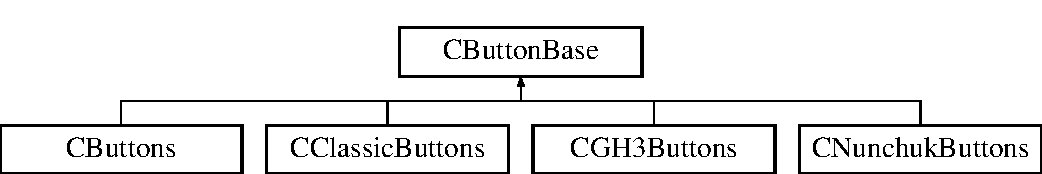
\includegraphics[height=2.000000cm]{class_c_button_base}
\end{center}
\end{figure}
\subsection*{\-Public \-Member \-Functions}
\begin{DoxyCompactItemize}
\item 
\hypertarget{class_c_button_base_a9c86334a1e2b3ba2c771b2e574c3dc67}{{\bfseries \-C\-Button\-Base} (void $\ast$\-Buttons\-Ptr, void $\ast$\-Buttons\-Held\-Ptr, void $\ast$\-Buttons\-Released\-Ptr)}\label{class_c_button_base_a9c86334a1e2b3ba2c771b2e574c3dc67}

\item 
\hypertarget{class_c_button_base_a0d4758b9e756a8c3c2bb39b907ea9170}{int {\bfseries is\-Pressed} (int \-Button)}\label{class_c_button_base_a0d4758b9e756a8c3c2bb39b907ea9170}

\item 
\hypertarget{class_c_button_base_a67e38daead9d22e33f6a3d85902d1f98}{int {\bfseries is\-Held} (int \-Button)}\label{class_c_button_base_a67e38daead9d22e33f6a3d85902d1f98}

\item 
\hypertarget{class_c_button_base_a575dee487bcca1abf29c1084dfdd5bb8}{int {\bfseries is\-Released} (int \-Button)}\label{class_c_button_base_a575dee487bcca1abf29c1084dfdd5bb8}

\item 
\hypertarget{class_c_button_base_ab74fd21217c5e379a613b7474af4f9b8}{int {\bfseries is\-Just\-Pressed} (int \-Button)}\label{class_c_button_base_ab74fd21217c5e379a613b7474af4f9b8}

\end{DoxyCompactItemize}
\subsection*{\-Private \-Member \-Functions}
\begin{DoxyCompactItemize}
\item 
\hypertarget{class_c_button_base_aa2accc210e6c60b8d4aec8ea5ee4a9d8}{virtual short {\bfseries \-Cast} (void $\ast$\-Ptr)}\label{class_c_button_base_aa2accc210e6c60b8d4aec8ea5ee4a9d8}

\end{DoxyCompactItemize}
\subsection*{\-Private \-Attributes}
\begin{DoxyCompactItemize}
\item 
\hypertarget{class_c_button_base_ac15590c3755869ab95aac1716e2f83b7}{void $\ast$ {\bfseries mp\-Btns\-Ptr}}\label{class_c_button_base_ac15590c3755869ab95aac1716e2f83b7}

\item 
\hypertarget{class_c_button_base_ab8c2766f06261ea74a6d8ae3f7cf52dd}{void $\ast$ {\bfseries mp\-Btns\-Held\-Ptr}}\label{class_c_button_base_ab8c2766f06261ea74a6d8ae3f7cf52dd}

\item 
\hypertarget{class_c_button_base_a8d064f3dc6b97b1b53067e4f35bd6367}{void $\ast$ {\bfseries mp\-Btns\-Released\-Ptr}}\label{class_c_button_base_a8d064f3dc6b97b1b53067e4f35bd6367}

\end{DoxyCompactItemize}


\subsection{\-Detailed \-Description}


\-Definition at line 43 of file wiicpp.\-h.



\-The documentation for this class was generated from the following files\-:\begin{DoxyCompactItemize}
\item 
wiicpp.\-h\item 
wiicpp.\-cpp\end{DoxyCompactItemize}

\hypertarget{class_c_buttons}{\section{C\-Buttons Class Reference}
\label{class_c_buttons}\index{C\-Buttons@{C\-Buttons}}
}
Inheritance diagram for C\-Buttons\-:\begin{figure}[H]
\begin{center}
\leavevmode
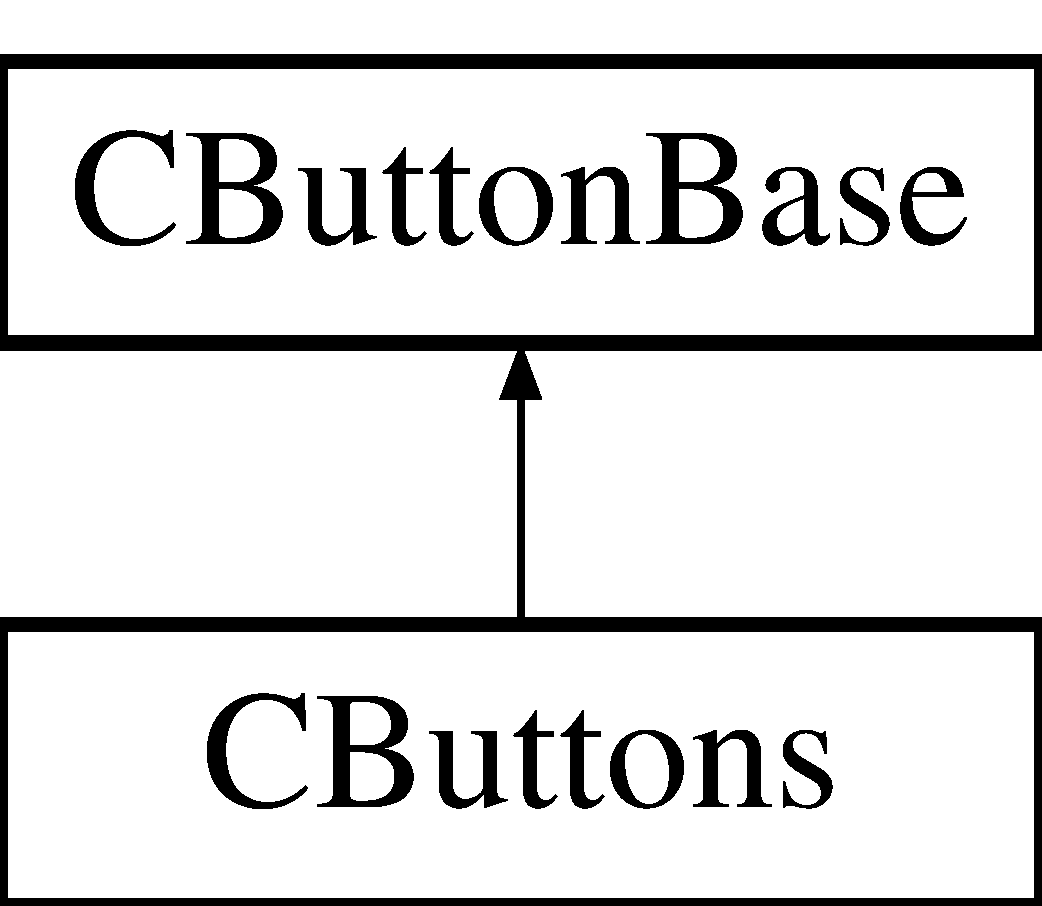
\includegraphics[height=2.000000cm]{class_c_buttons}
\end{center}
\end{figure}
\subsection*{Public Types}
\begin{DoxyCompactItemize}
\item 
enum {\bfseries Button\-Defs} \{ \\*
{\bfseries B\-U\-T\-T\-O\-N\-\_\-\-T\-W\-O} =  W\-I\-I\-M\-O\-T\-E\-\_\-\-B\-U\-T\-T\-O\-N\-\_\-\-T\-W\-O, 
{\bfseries B\-U\-T\-T\-O\-N\-\_\-\-O\-N\-E} =  W\-I\-I\-M\-O\-T\-E\-\_\-\-B\-U\-T\-T\-O\-N\-\_\-\-O\-N\-E, 
{\bfseries B\-U\-T\-T\-O\-N\-\_\-\-B} =  W\-I\-I\-M\-O\-T\-E\-\_\-\-B\-U\-T\-T\-O\-N\-\_\-\-B, 
{\bfseries B\-U\-T\-T\-O\-N\-\_\-\-A} =  W\-I\-I\-M\-O\-T\-E\-\_\-\-B\-U\-T\-T\-O\-N\-\_\-\-A, 
\\*
{\bfseries B\-U\-T\-T\-O\-N\-\_\-\-M\-I\-N\-U\-S} =  W\-I\-I\-M\-O\-T\-E\-\_\-\-B\-U\-T\-T\-O\-N\-\_\-\-M\-I\-N\-U\-S, 
{\bfseries B\-U\-T\-T\-O\-N\-\_\-\-H\-O\-M\-E} =  W\-I\-I\-M\-O\-T\-E\-\_\-\-B\-U\-T\-T\-O\-N\-\_\-\-H\-O\-M\-E, 
{\bfseries B\-U\-T\-T\-O\-N\-\_\-\-L\-E\-F\-T} =  W\-I\-I\-M\-O\-T\-E\-\_\-\-B\-U\-T\-T\-O\-N\-\_\-\-L\-E\-F\-T, 
{\bfseries B\-U\-T\-T\-O\-N\-\_\-\-R\-I\-G\-H\-T} =  W\-I\-I\-M\-O\-T\-E\-\_\-\-B\-U\-T\-T\-O\-N\-\_\-\-R\-I\-G\-H\-T, 
\\*
{\bfseries B\-U\-T\-T\-O\-N\-\_\-\-D\-O\-W\-N} =  W\-I\-I\-M\-O\-T\-E\-\_\-\-B\-U\-T\-T\-O\-N\-\_\-\-D\-O\-W\-N, 
{\bfseries B\-U\-T\-T\-O\-N\-\_\-\-U\-P} =  W\-I\-I\-M\-O\-T\-E\-\_\-\-B\-U\-T\-T\-O\-N\-\_\-\-U\-P, 
{\bfseries B\-U\-T\-T\-O\-N\-\_\-\-P\-L\-U\-S} =  W\-I\-I\-M\-O\-T\-E\-\_\-\-B\-U\-T\-T\-O\-N\-\_\-\-P\-L\-U\-S, 
{\bfseries B\-U\-T\-T\-O\-N\-\_\-\-U\-N\-K\-N\-O\-W\-N} =  W\-I\-I\-M\-O\-T\-E\-\_\-\-B\-U\-T\-T\-O\-N\-\_\-\-U\-N\-K\-N\-O\-W\-N, 
\\*
{\bfseries B\-U\-T\-T\-O\-N\-\_\-\-A\-L\-L} =  W\-I\-I\-M\-O\-T\-E\-\_\-\-B\-U\-T\-T\-O\-N\-\_\-\-A\-L\-L, 
{\bfseries B\-U\-T\-T\-O\-N\-\_\-\-T\-W\-O} =  W\-I\-I\-M\-O\-T\-E\-\_\-\-B\-U\-T\-T\-O\-N\-\_\-\-T\-W\-O, 
{\bfseries B\-U\-T\-T\-O\-N\-\_\-\-O\-N\-E} =  W\-I\-I\-M\-O\-T\-E\-\_\-\-B\-U\-T\-T\-O\-N\-\_\-\-O\-N\-E, 
{\bfseries B\-U\-T\-T\-O\-N\-\_\-\-B} =  W\-I\-I\-M\-O\-T\-E\-\_\-\-B\-U\-T\-T\-O\-N\-\_\-\-B, 
\\*
{\bfseries B\-U\-T\-T\-O\-N\-\_\-\-A} =  W\-I\-I\-M\-O\-T\-E\-\_\-\-B\-U\-T\-T\-O\-N\-\_\-\-A, 
{\bfseries B\-U\-T\-T\-O\-N\-\_\-\-M\-I\-N\-U\-S} =  W\-I\-I\-M\-O\-T\-E\-\_\-\-B\-U\-T\-T\-O\-N\-\_\-\-M\-I\-N\-U\-S, 
{\bfseries B\-U\-T\-T\-O\-N\-\_\-\-H\-O\-M\-E} =  W\-I\-I\-M\-O\-T\-E\-\_\-\-B\-U\-T\-T\-O\-N\-\_\-\-H\-O\-M\-E, 
{\bfseries B\-U\-T\-T\-O\-N\-\_\-\-L\-E\-F\-T} =  W\-I\-I\-M\-O\-T\-E\-\_\-\-B\-U\-T\-T\-O\-N\-\_\-\-L\-E\-F\-T, 
\\*
{\bfseries B\-U\-T\-T\-O\-N\-\_\-\-R\-I\-G\-H\-T} =  W\-I\-I\-M\-O\-T\-E\-\_\-\-B\-U\-T\-T\-O\-N\-\_\-\-R\-I\-G\-H\-T, 
{\bfseries B\-U\-T\-T\-O\-N\-\_\-\-D\-O\-W\-N} =  W\-I\-I\-M\-O\-T\-E\-\_\-\-B\-U\-T\-T\-O\-N\-\_\-\-D\-O\-W\-N, 
{\bfseries B\-U\-T\-T\-O\-N\-\_\-\-U\-P} =  W\-I\-I\-M\-O\-T\-E\-\_\-\-B\-U\-T\-T\-O\-N\-\_\-\-U\-P, 
{\bfseries B\-U\-T\-T\-O\-N\-\_\-\-P\-L\-U\-S} =  W\-I\-I\-M\-O\-T\-E\-\_\-\-B\-U\-T\-T\-O\-N\-\_\-\-P\-L\-U\-S, 
\\*
{\bfseries B\-U\-T\-T\-O\-N\-\_\-\-U\-N\-K\-N\-O\-W\-N} =  W\-I\-I\-M\-O\-T\-E\-\_\-\-B\-U\-T\-T\-O\-N\-\_\-\-U\-N\-K\-N\-O\-W\-N, 
{\bfseries B\-U\-T\-T\-O\-N\-\_\-\-A\-L\-L} =  W\-I\-I\-M\-O\-T\-E\-\_\-\-B\-U\-T\-T\-O\-N\-\_\-\-A\-L\-L
 \}
\item 
enum {\bfseries Button\-Defs} \{ \\*
{\bfseries B\-U\-T\-T\-O\-N\-\_\-\-T\-W\-O} =  W\-I\-I\-M\-O\-T\-E\-\_\-\-B\-U\-T\-T\-O\-N\-\_\-\-T\-W\-O, 
{\bfseries B\-U\-T\-T\-O\-N\-\_\-\-O\-N\-E} =  W\-I\-I\-M\-O\-T\-E\-\_\-\-B\-U\-T\-T\-O\-N\-\_\-\-O\-N\-E, 
{\bfseries B\-U\-T\-T\-O\-N\-\_\-\-B} =  W\-I\-I\-M\-O\-T\-E\-\_\-\-B\-U\-T\-T\-O\-N\-\_\-\-B, 
{\bfseries B\-U\-T\-T\-O\-N\-\_\-\-A} =  W\-I\-I\-M\-O\-T\-E\-\_\-\-B\-U\-T\-T\-O\-N\-\_\-\-A, 
\\*
{\bfseries B\-U\-T\-T\-O\-N\-\_\-\-M\-I\-N\-U\-S} =  W\-I\-I\-M\-O\-T\-E\-\_\-\-B\-U\-T\-T\-O\-N\-\_\-\-M\-I\-N\-U\-S, 
{\bfseries B\-U\-T\-T\-O\-N\-\_\-\-H\-O\-M\-E} =  W\-I\-I\-M\-O\-T\-E\-\_\-\-B\-U\-T\-T\-O\-N\-\_\-\-H\-O\-M\-E, 
{\bfseries B\-U\-T\-T\-O\-N\-\_\-\-L\-E\-F\-T} =  W\-I\-I\-M\-O\-T\-E\-\_\-\-B\-U\-T\-T\-O\-N\-\_\-\-L\-E\-F\-T, 
{\bfseries B\-U\-T\-T\-O\-N\-\_\-\-R\-I\-G\-H\-T} =  W\-I\-I\-M\-O\-T\-E\-\_\-\-B\-U\-T\-T\-O\-N\-\_\-\-R\-I\-G\-H\-T, 
\\*
{\bfseries B\-U\-T\-T\-O\-N\-\_\-\-D\-O\-W\-N} =  W\-I\-I\-M\-O\-T\-E\-\_\-\-B\-U\-T\-T\-O\-N\-\_\-\-D\-O\-W\-N, 
{\bfseries B\-U\-T\-T\-O\-N\-\_\-\-U\-P} =  W\-I\-I\-M\-O\-T\-E\-\_\-\-B\-U\-T\-T\-O\-N\-\_\-\-U\-P, 
{\bfseries B\-U\-T\-T\-O\-N\-\_\-\-P\-L\-U\-S} =  W\-I\-I\-M\-O\-T\-E\-\_\-\-B\-U\-T\-T\-O\-N\-\_\-\-P\-L\-U\-S, 
{\bfseries B\-U\-T\-T\-O\-N\-\_\-\-U\-N\-K\-N\-O\-W\-N} =  W\-I\-I\-M\-O\-T\-E\-\_\-\-B\-U\-T\-T\-O\-N\-\_\-\-U\-N\-K\-N\-O\-W\-N, 
\\*
{\bfseries B\-U\-T\-T\-O\-N\-\_\-\-A\-L\-L} =  W\-I\-I\-M\-O\-T\-E\-\_\-\-B\-U\-T\-T\-O\-N\-\_\-\-A\-L\-L, 
{\bfseries B\-U\-T\-T\-O\-N\-\_\-\-T\-W\-O} =  W\-I\-I\-M\-O\-T\-E\-\_\-\-B\-U\-T\-T\-O\-N\-\_\-\-T\-W\-O, 
{\bfseries B\-U\-T\-T\-O\-N\-\_\-\-O\-N\-E} =  W\-I\-I\-M\-O\-T\-E\-\_\-\-B\-U\-T\-T\-O\-N\-\_\-\-O\-N\-E, 
{\bfseries B\-U\-T\-T\-O\-N\-\_\-\-B} =  W\-I\-I\-M\-O\-T\-E\-\_\-\-B\-U\-T\-T\-O\-N\-\_\-\-B, 
\\*
{\bfseries B\-U\-T\-T\-O\-N\-\_\-\-A} =  W\-I\-I\-M\-O\-T\-E\-\_\-\-B\-U\-T\-T\-O\-N\-\_\-\-A, 
{\bfseries B\-U\-T\-T\-O\-N\-\_\-\-M\-I\-N\-U\-S} =  W\-I\-I\-M\-O\-T\-E\-\_\-\-B\-U\-T\-T\-O\-N\-\_\-\-M\-I\-N\-U\-S, 
{\bfseries B\-U\-T\-T\-O\-N\-\_\-\-H\-O\-M\-E} =  W\-I\-I\-M\-O\-T\-E\-\_\-\-B\-U\-T\-T\-O\-N\-\_\-\-H\-O\-M\-E, 
{\bfseries B\-U\-T\-T\-O\-N\-\_\-\-L\-E\-F\-T} =  W\-I\-I\-M\-O\-T\-E\-\_\-\-B\-U\-T\-T\-O\-N\-\_\-\-L\-E\-F\-T, 
\\*
{\bfseries B\-U\-T\-T\-O\-N\-\_\-\-R\-I\-G\-H\-T} =  W\-I\-I\-M\-O\-T\-E\-\_\-\-B\-U\-T\-T\-O\-N\-\_\-\-R\-I\-G\-H\-T, 
{\bfseries B\-U\-T\-T\-O\-N\-\_\-\-D\-O\-W\-N} =  W\-I\-I\-M\-O\-T\-E\-\_\-\-B\-U\-T\-T\-O\-N\-\_\-\-D\-O\-W\-N, 
{\bfseries B\-U\-T\-T\-O\-N\-\_\-\-U\-P} =  W\-I\-I\-M\-O\-T\-E\-\_\-\-B\-U\-T\-T\-O\-N\-\_\-\-U\-P, 
{\bfseries B\-U\-T\-T\-O\-N\-\_\-\-P\-L\-U\-S} =  W\-I\-I\-M\-O\-T\-E\-\_\-\-B\-U\-T\-T\-O\-N\-\_\-\-P\-L\-U\-S, 
\\*
{\bfseries B\-U\-T\-T\-O\-N\-\_\-\-U\-N\-K\-N\-O\-W\-N} =  W\-I\-I\-M\-O\-T\-E\-\_\-\-B\-U\-T\-T\-O\-N\-\_\-\-U\-N\-K\-N\-O\-W\-N, 
{\bfseries B\-U\-T\-T\-O\-N\-\_\-\-A\-L\-L} =  W\-I\-I\-M\-O\-T\-E\-\_\-\-B\-U\-T\-T\-O\-N\-\_\-\-A\-L\-L
 \}
\end{DoxyCompactItemize}
\subsection*{Public Member Functions}
\begin{DoxyCompactItemize}
\item 
\hypertarget{class_c_buttons_ae5c226df45be410d158a792510af7f17}{{\bfseries C\-Buttons} (void $\ast$Buttons\-Ptr, void $\ast$Buttons\-Held\-Ptr, void $\ast$Buttons\-Released\-Ptr)}\label{class_c_buttons_ae5c226df45be410d158a792510af7f17}

\item 
\hypertarget{class_c_buttons_ae5c226df45be410d158a792510af7f17}{{\bfseries C\-Buttons} (void $\ast$Buttons\-Ptr, void $\ast$Buttons\-Held\-Ptr, void $\ast$Buttons\-Released\-Ptr)}\label{class_c_buttons_ae5c226df45be410d158a792510af7f17}

\item 
\hypertarget{class_c_button_base_a0d4758b9e756a8c3c2bb39b907ea9170}{int {\bfseries is\-Pressed} (int Button)}\label{class_c_button_base_a0d4758b9e756a8c3c2bb39b907ea9170}

\item 
\hypertarget{class_c_button_base_a0d4758b9e756a8c3c2bb39b907ea9170}{int {\bfseries is\-Pressed} (int Button)}\label{class_c_button_base_a0d4758b9e756a8c3c2bb39b907ea9170}

\item 
\hypertarget{class_c_button_base_a67e38daead9d22e33f6a3d85902d1f98}{int {\bfseries is\-Held} (int Button)}\label{class_c_button_base_a67e38daead9d22e33f6a3d85902d1f98}

\item 
\hypertarget{class_c_button_base_a67e38daead9d22e33f6a3d85902d1f98}{int {\bfseries is\-Held} (int Button)}\label{class_c_button_base_a67e38daead9d22e33f6a3d85902d1f98}

\item 
\hypertarget{class_c_button_base_a575dee487bcca1abf29c1084dfdd5bb8}{int {\bfseries is\-Released} (int Button)}\label{class_c_button_base_a575dee487bcca1abf29c1084dfdd5bb8}

\item 
\hypertarget{class_c_button_base_a575dee487bcca1abf29c1084dfdd5bb8}{int {\bfseries is\-Released} (int Button)}\label{class_c_button_base_a575dee487bcca1abf29c1084dfdd5bb8}

\item 
\hypertarget{class_c_button_base_ab74fd21217c5e379a613b7474af4f9b8}{int {\bfseries is\-Just\-Pressed} (int Button)}\label{class_c_button_base_ab74fd21217c5e379a613b7474af4f9b8}

\item 
\hypertarget{class_c_button_base_ab74fd21217c5e379a613b7474af4f9b8}{int {\bfseries is\-Just\-Pressed} (int Button)}\label{class_c_button_base_ab74fd21217c5e379a613b7474af4f9b8}

\end{DoxyCompactItemize}


\subsection{Detailed Description}


Definition at line 61 of file wiic\-\_\-r90/src/wiicpp/wiicpp.\-h.



The documentation for this class was generated from the following files\-:\begin{DoxyCompactItemize}
\item 
wiic\-\_\-r90/src/wiicpp/wiicpp.\-h\item 
wiic\-\_\-v1.\-1/src/wiicpp/wiicpp.\-h\item 
wiic\-\_\-r90/src/wiicpp/wiicpp.\-cpp\item 
wiic\-\_\-v1.\-1/src/wiicpp/wiicpp.\-cpp\end{DoxyCompactItemize}

\hypertarget{class_c_classic}{\section{\-C\-Classic \-Class \-Reference}
\label{class_c_classic}\index{\-C\-Classic@{\-C\-Classic}}
}
\subsection*{\-Public \-Member \-Functions}
\begin{DoxyCompactItemize}
\item 
\hypertarget{class_c_classic_ac682fe2a19e88a0dd1fff9a12586d6e2}{{\bfseries \-C\-Classic} (struct \hyperlink{structexpansion__t}{expansion\-\_\-t} $\ast$\-Exp\-Ptr)}\label{class_c_classic_ac682fe2a19e88a0dd1fff9a12586d6e2}

\item 
\hypertarget{class_c_classic_a7ea18d3535fb4534790a6b24e33e8c56}{float {\bfseries \-Get\-L\-Shoulder\-Button} ()}\label{class_c_classic_a7ea18d3535fb4534790a6b24e33e8c56}

\item 
\hypertarget{class_c_classic_a58ac294e9273589037f60a1d2e4fcfac}{float {\bfseries \-Get\-R\-Shoulder\-Button} ()}\label{class_c_classic_a58ac294e9273589037f60a1d2e4fcfac}

\end{DoxyCompactItemize}
\subsection*{\-Public \-Attributes}
\begin{DoxyCompactItemize}
\item 
\hypertarget{class_c_classic_a1592d3c639fa90e657cc3c3f741363b8}{\hyperlink{class_c_classic_buttons}{\-C\-Classic\-Buttons} {\bfseries \-Buttons}}\label{class_c_classic_a1592d3c639fa90e657cc3c3f741363b8}

\item 
\hypertarget{class_c_classic_a3469e965eac46db5ecc669d74d8a2420}{\hyperlink{class_c_joystick}{\-C\-Joystick} {\bfseries \-Left\-Joystick}}\label{class_c_classic_a3469e965eac46db5ecc669d74d8a2420}

\item 
\hypertarget{class_c_classic_a65a96a9397c278e0bc5e7f5b7048d855}{\hyperlink{class_c_joystick}{\-C\-Joystick} {\bfseries \-Right\-Joystick}}\label{class_c_classic_a65a96a9397c278e0bc5e7f5b7048d855}

\end{DoxyCompactItemize}
\subsection*{\-Private \-Attributes}
\begin{DoxyCompactItemize}
\item 
\hypertarget{class_c_classic_a6fd9bbfe830df5a3daed2c912b593f02}{struct \hyperlink{structclassic__ctrl__t}{classic\-\_\-ctrl\-\_\-t} $\ast$ {\bfseries mp\-Classic\-Ptr}}\label{class_c_classic_a6fd9bbfe830df5a3daed2c912b593f02}

\end{DoxyCompactItemize}


\subsection{\-Detailed \-Description}


\-Definition at line 318 of file wiicpp.\-h.



\-The documentation for this class was generated from the following files\-:\begin{DoxyCompactItemize}
\item 
wiicpp.\-h\item 
wiicpp.\-cpp\end{DoxyCompactItemize}

\hypertarget{class_c_classic_buttons}{\section{\-C\-Classic\-Buttons \-Class \-Reference}
\label{class_c_classic_buttons}\index{\-C\-Classic\-Buttons@{\-C\-Classic\-Buttons}}
}
\-Inheritance diagram for \-C\-Classic\-Buttons\-:\begin{figure}[H]
\begin{center}
\leavevmode
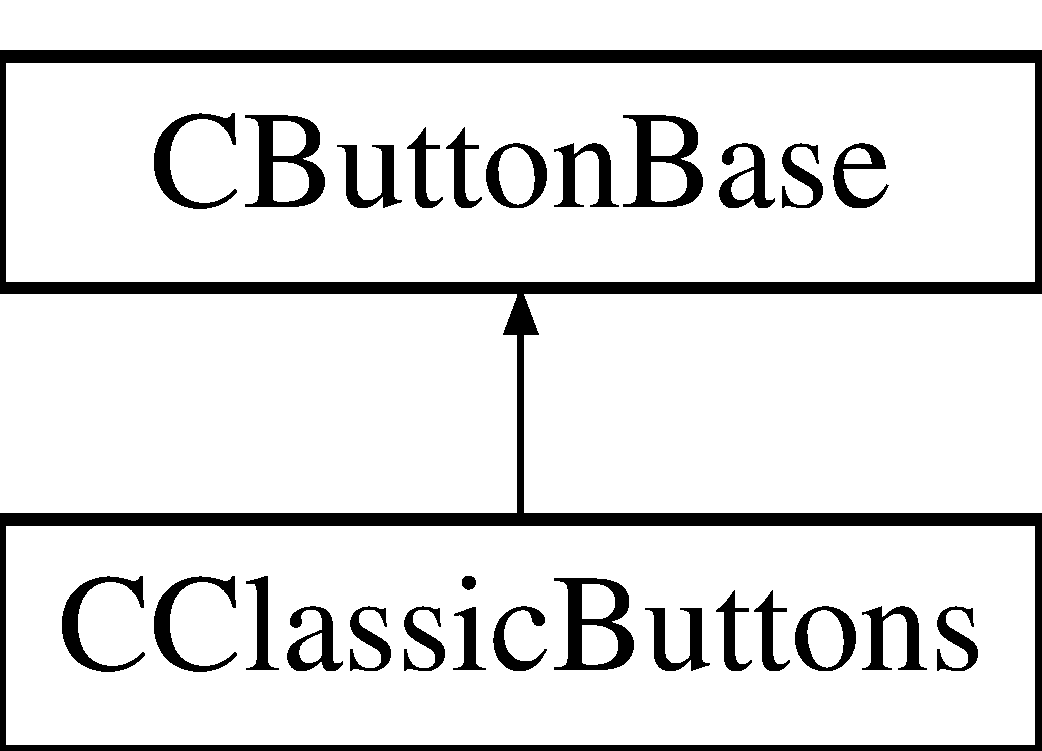
\includegraphics[height=2.000000cm]{class_c_classic_buttons}
\end{center}
\end{figure}
\subsection*{\-Public \-Types}
\begin{DoxyCompactItemize}
\item 
enum {\bfseries \-Button\-Defs} \{ \*
{\bfseries \-B\-U\-T\-T\-O\-N\-\_\-\-X} =  \-C\-L\-A\-S\-S\-I\-C\-\_\-\-C\-T\-R\-L\-\_\-\-B\-U\-T\-T\-O\-N\-\_\-\-X, 
{\bfseries \-B\-U\-T\-T\-O\-N\-\_\-\-Y} =  \-C\-L\-A\-S\-S\-I\-C\-\_\-\-C\-T\-R\-L\-\_\-\-B\-U\-T\-T\-O\-N\-\_\-\-Y, 
{\bfseries \-B\-U\-T\-T\-O\-N\-\_\-\-B} =  \-C\-L\-A\-S\-S\-I\-C\-\_\-\-C\-T\-R\-L\-\_\-\-B\-U\-T\-T\-O\-N\-\_\-\-B, 
{\bfseries \-B\-U\-T\-T\-O\-N\-\_\-\-A} =  \-C\-L\-A\-S\-S\-I\-C\-\_\-\-C\-T\-R\-L\-\_\-\-B\-U\-T\-T\-O\-N\-\_\-\-A, 
\*
{\bfseries \-B\-U\-T\-T\-O\-N\-\_\-\-M\-I\-N\-U\-S} =  \-C\-L\-A\-S\-S\-I\-C\-\_\-\-C\-T\-R\-L\-\_\-\-B\-U\-T\-T\-O\-N\-\_\-\-M\-I\-N\-U\-S, 
{\bfseries \-B\-U\-T\-T\-O\-N\-\_\-\-H\-O\-M\-E} =  \-C\-L\-A\-S\-S\-I\-C\-\_\-\-C\-T\-R\-L\-\_\-\-B\-U\-T\-T\-O\-N\-\_\-\-H\-O\-M\-E, 
{\bfseries \-B\-U\-T\-T\-O\-N\-\_\-\-L\-E\-F\-T} =  \-C\-L\-A\-S\-S\-I\-C\-\_\-\-C\-T\-R\-L\-\_\-\-B\-U\-T\-T\-O\-N\-\_\-\-L\-E\-F\-T, 
{\bfseries \-B\-U\-T\-T\-O\-N\-\_\-\-R\-I\-G\-H\-T} =  \-C\-L\-A\-S\-S\-I\-C\-\_\-\-C\-T\-R\-L\-\_\-\-B\-U\-T\-T\-O\-N\-\_\-\-R\-I\-G\-H\-T, 
\*
{\bfseries \-B\-U\-T\-T\-O\-N\-\_\-\-D\-O\-W\-N} =  \-C\-L\-A\-S\-S\-I\-C\-\_\-\-C\-T\-R\-L\-\_\-\-B\-U\-T\-T\-O\-N\-\_\-\-D\-O\-W\-N, 
{\bfseries \-B\-U\-T\-T\-O\-N\-\_\-\-U\-P} =  \-C\-L\-A\-S\-S\-I\-C\-\_\-\-C\-T\-R\-L\-\_\-\-B\-U\-T\-T\-O\-N\-\_\-\-U\-P, 
{\bfseries \-B\-U\-T\-T\-O\-N\-\_\-\-P\-L\-U\-S} =  \-C\-L\-A\-S\-S\-I\-C\-\_\-\-C\-T\-R\-L\-\_\-\-B\-U\-T\-T\-O\-N\-\_\-\-P\-L\-U\-S, 
{\bfseries \-B\-U\-T\-T\-O\-N\-\_\-\-Z\-R} =  \-C\-L\-A\-S\-S\-I\-C\-\_\-\-C\-T\-R\-L\-\_\-\-B\-U\-T\-T\-O\-N\-\_\-\-Z\-R, 
\*
{\bfseries \-B\-U\-T\-T\-O\-N\-\_\-\-Z\-L} =  \-C\-L\-A\-S\-S\-I\-C\-\_\-\-C\-T\-R\-L\-\_\-\-B\-U\-T\-T\-O\-N\-\_\-\-Z\-L, 
{\bfseries \-B\-U\-T\-T\-O\-N\-\_\-\-F\-U\-L\-L\-\_\-\-R} =  \-C\-L\-A\-S\-S\-I\-C\-\_\-\-C\-T\-R\-L\-\_\-\-B\-U\-T\-T\-O\-N\-\_\-\-F\-U\-L\-L\-\_\-\-R, 
{\bfseries \-B\-U\-T\-T\-O\-N\-\_\-\-F\-U\-L\-L\-\_\-\-L} =  \-C\-L\-A\-S\-S\-I\-C\-\_\-\-C\-T\-R\-L\-\_\-\-B\-U\-T\-T\-O\-N\-\_\-\-F\-U\-L\-L\-\_\-\-L, 
{\bfseries \-B\-U\-T\-T\-O\-N\-\_\-\-A\-L\-L} =  \-C\-L\-A\-S\-S\-I\-C\-\_\-\-C\-T\-R\-L\-\_\-\-B\-U\-T\-T\-O\-N\-\_\-\-A\-L\-L
 \}
\end{DoxyCompactItemize}
\subsection*{\-Public \-Member \-Functions}
\begin{DoxyCompactItemize}
\item 
\hypertarget{class_c_classic_buttons_ae98fc8217e2e7a38e9393be008534268}{{\bfseries \-C\-Classic\-Buttons} (void $\ast$\-Buttons\-Ptr, void $\ast$\-Buttons\-Held\-Ptr, void $\ast$\-Buttons\-Released\-Ptr)}\label{class_c_classic_buttons_ae98fc8217e2e7a38e9393be008534268}

\item 
\hypertarget{class_c_button_base_a0d4758b9e756a8c3c2bb39b907ea9170}{int {\bfseries is\-Pressed} (int \-Button)}\label{class_c_button_base_a0d4758b9e756a8c3c2bb39b907ea9170}

\item 
\hypertarget{class_c_button_base_a67e38daead9d22e33f6a3d85902d1f98}{int {\bfseries is\-Held} (int \-Button)}\label{class_c_button_base_a67e38daead9d22e33f6a3d85902d1f98}

\item 
\hypertarget{class_c_button_base_a575dee487bcca1abf29c1084dfdd5bb8}{int {\bfseries is\-Released} (int \-Button)}\label{class_c_button_base_a575dee487bcca1abf29c1084dfdd5bb8}

\item 
\hypertarget{class_c_button_base_ab74fd21217c5e379a613b7474af4f9b8}{int {\bfseries is\-Just\-Pressed} (int \-Button)}\label{class_c_button_base_ab74fd21217c5e379a613b7474af4f9b8}

\end{DoxyCompactItemize}


\subsection{\-Detailed \-Description}


\-Definition at line 100 of file wiicpp.\-h.



\-The documentation for this class was generated from the following files\-:\begin{DoxyCompactItemize}
\item 
wiicpp.\-h\item 
wiicpp.\-cpp\end{DoxyCompactItemize}

\hypertarget{class_c_expansion_device}{\section{C\-Expansion\-Device Class Reference}
\label{class_c_expansion_device}\index{C\-Expansion\-Device@{C\-Expansion\-Device}}
}
\subsection*{Public Types}
\begin{DoxyCompactItemize}
\item 
enum {\bfseries Exp\-Types} \{ \\*
{\bfseries T\-Y\-P\-E\-\_\-\-N\-O\-N\-E} =  E\-X\-P\-\_\-\-N\-O\-N\-E, 
{\bfseries T\-Y\-P\-E\-\_\-\-N\-U\-N\-C\-H\-U\-K} =  E\-X\-P\-\_\-\-N\-U\-N\-C\-H\-U\-K, 
{\bfseries T\-Y\-P\-E\-\_\-\-C\-L\-A\-S\-S\-I\-C} =  E\-X\-P\-\_\-\-C\-L\-A\-S\-S\-I\-C, 
{\bfseries T\-Y\-P\-E\-\_\-\-G\-U\-I\-T\-A\-R\-\_\-\-H\-E\-R\-O\-\_\-3} =  E\-X\-P\-\_\-\-G\-U\-I\-T\-A\-R\-\_\-\-H\-E\-R\-O\-\_\-3, 
\\*
{\bfseries T\-Y\-P\-E\-\_\-\-M\-O\-T\-I\-O\-N\-\_\-\-P\-L\-U\-S} =  E\-X\-P\-\_\-\-M\-O\-T\-I\-O\-N\-\_\-\-P\-L\-U\-S, 
{\bfseries T\-Y\-P\-E\-\_\-\-B\-A\-L\-A\-N\-C\-E\-\_\-\-B\-O\-A\-R\-D} =  E\-X\-P\-\_\-\-B\-A\-L\-A\-N\-C\-E\-\_\-\-B\-O\-A\-R\-D
 \}
\end{DoxyCompactItemize}
\subsection*{Public Member Functions}
\begin{DoxyCompactItemize}
\item 
\hypertarget{class_c_expansion_device_a68809e7c5c3736cc307e48630a7168a0}{{\bfseries C\-Expansion\-Device} (struct \hyperlink{structexpansion__t}{expansion\-\_\-t} $\ast$Exp\-Ptr)}\label{class_c_expansion_device_a68809e7c5c3736cc307e48630a7168a0}

\item 
\hypertarget{class_c_expansion_device_afe34f8c67883e2283b87332aed1b372f}{Exp\-Types {\bfseries Get\-Type} ()}\label{class_c_expansion_device_afe34f8c67883e2283b87332aed1b372f}

\end{DoxyCompactItemize}
\subsection*{Public Attributes}
\begin{DoxyCompactItemize}
\item 
\hypertarget{class_c_expansion_device_a9a30f45df41f2e0457fe3f57c0f0f53e}{\hyperlink{class_c_nunchuk}{C\-Nunchuk} {\bfseries Nunchuk}}\label{class_c_expansion_device_a9a30f45df41f2e0457fe3f57c0f0f53e}

\item 
\hypertarget{class_c_expansion_device_a2d84fd3250518acbcb28c733277a9931}{\hyperlink{class_c_classic}{C\-Classic} {\bfseries Classic}}\label{class_c_expansion_device_a2d84fd3250518acbcb28c733277a9931}

\item 
\hypertarget{class_c_expansion_device_a9ebd876c248d2b0242bf06181735a4e1}{\hyperlink{class_c_guitar_hero3}{C\-Guitar\-Hero3} {\bfseries Guitar\-Hero3}}\label{class_c_expansion_device_a9ebd876c248d2b0242bf06181735a4e1}

\item 
\hypertarget{class_c_expansion_device_a49310ff81cc6b9ac43839cb7f596cfa2}{\hyperlink{class_c_motion_plus}{C\-Motion\-Plus} {\bfseries Motion\-Plus}}\label{class_c_expansion_device_a49310ff81cc6b9ac43839cb7f596cfa2}

\item 
\hypertarget{class_c_expansion_device_aae5430823c39c8e8b836200b9b29ac42}{\hyperlink{class_c_balance_board}{C\-Balance\-Board} {\bfseries Balance\-Board}}\label{class_c_expansion_device_aae5430823c39c8e8b836200b9b29ac42}

\end{DoxyCompactItemize}
\subsection*{Private Attributes}
\begin{DoxyCompactItemize}
\item 
\hypertarget{class_c_expansion_device_a14884d7764e4c850f61c34f45ed2b97c}{struct \hyperlink{structexpansion__t}{expansion\-\_\-t} $\ast$ {\bfseries mp\-Expansion\-Ptr}}\label{class_c_expansion_device_a14884d7764e4c850f61c34f45ed2b97c}

\end{DoxyCompactItemize}


\subsection{Detailed Description}


Definition at line 372 of file wiicpp.\-h.



The documentation for this class was generated from the following files\-:\begin{DoxyCompactItemize}
\item 
wiicpp.\-h\item 
wiicpp.\-cpp\end{DoxyCompactItemize}

\hypertarget{class_c_g_h3_buttons}{\section{\-C\-G\-H3\-Buttons \-Class \-Reference}
\label{class_c_g_h3_buttons}\index{\-C\-G\-H3\-Buttons@{\-C\-G\-H3\-Buttons}}
}
\-Inheritance diagram for \-C\-G\-H3\-Buttons\-:\begin{figure}[H]
\begin{center}
\leavevmode
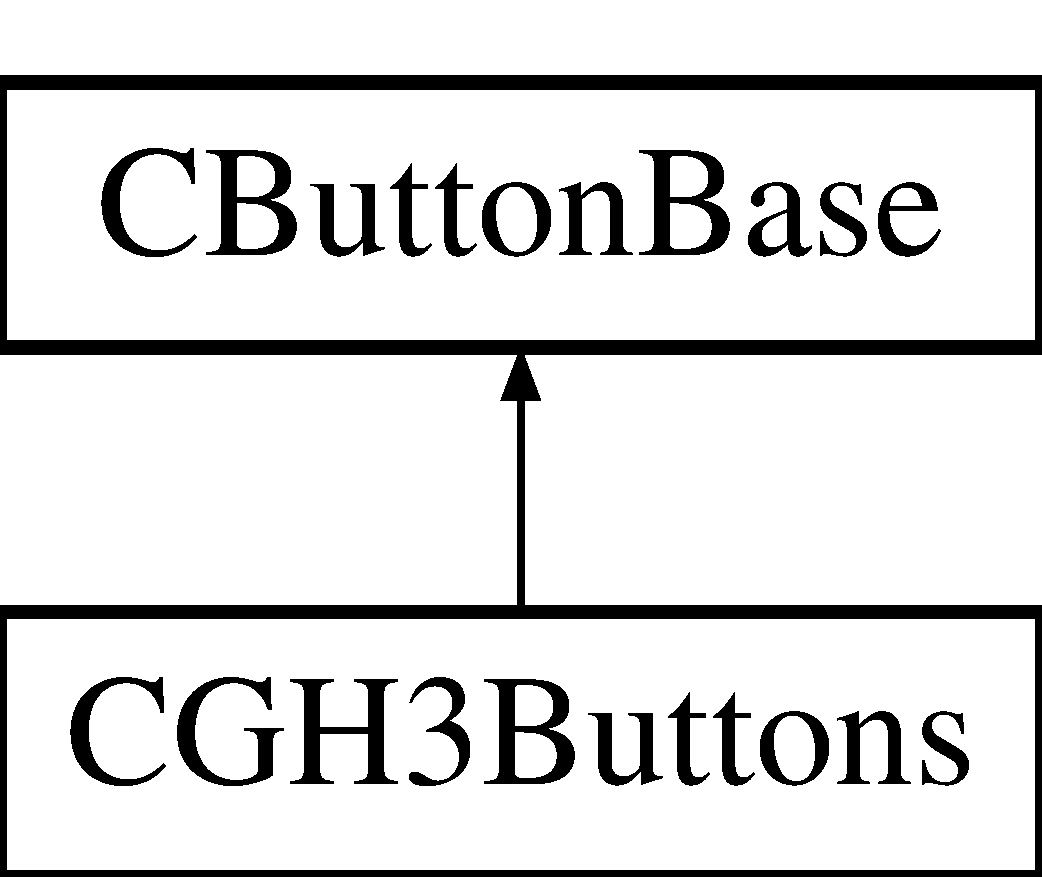
\includegraphics[height=2.000000cm]{class_c_g_h3_buttons}
\end{center}
\end{figure}
\subsection*{\-Public \-Types}
\begin{DoxyCompactItemize}
\item 
enum {\bfseries \-Button\-Defs} \{ \*
{\bfseries \-B\-U\-T\-T\-O\-N\-\_\-\-S\-T\-R\-U\-M\-\_\-\-U\-P} =  \-G\-U\-I\-T\-A\-R\-\_\-\-H\-E\-R\-O\-\_\-3\-\_\-\-B\-U\-T\-T\-O\-N\-\_\-\-S\-T\-R\-U\-M\-\_\-\-U\-P, 
{\bfseries \-B\-U\-T\-T\-O\-N\-\_\-\-S\-T\-R\-U\-M\-\_\-\-D\-O\-W\-N} =  \-G\-U\-I\-T\-A\-R\-\_\-\-H\-E\-R\-O\-\_\-3\-\_\-\-B\-U\-T\-T\-O\-N\-\_\-\-S\-T\-R\-U\-M\-\_\-\-D\-O\-W\-N, 
{\bfseries \-B\-U\-T\-T\-O\-N\-\_\-\-Y\-E\-L\-L\-O\-W} =  \-G\-U\-I\-T\-A\-R\-\_\-\-H\-E\-R\-O\-\_\-3\-\_\-\-B\-U\-T\-T\-O\-N\-\_\-\-Y\-E\-L\-L\-O\-W, 
{\bfseries \-B\-U\-T\-T\-O\-N\-\_\-\-G\-R\-E\-E\-N} =  \-G\-U\-I\-T\-A\-R\-\_\-\-H\-E\-R\-O\-\_\-3\-\_\-\-B\-U\-T\-T\-O\-N\-\_\-\-G\-R\-E\-E\-N, 
\*
{\bfseries \-B\-U\-T\-T\-O\-N\-\_\-\-B\-L\-U\-E} =  \-G\-U\-I\-T\-A\-R\-\_\-\-H\-E\-R\-O\-\_\-3\-\_\-\-B\-U\-T\-T\-O\-N\-\_\-\-B\-L\-U\-E, 
{\bfseries \-B\-U\-T\-T\-O\-N\-\_\-\-R\-E\-D} =  \-G\-U\-I\-T\-A\-R\-\_\-\-H\-E\-R\-O\-\_\-3\-\_\-\-B\-U\-T\-T\-O\-N\-\_\-\-R\-E\-D, 
{\bfseries \-B\-U\-T\-T\-O\-N\-\_\-\-O\-R\-A\-N\-G\-E} =  \-G\-U\-I\-T\-A\-R\-\_\-\-H\-E\-R\-O\-\_\-3\-\_\-\-B\-U\-T\-T\-O\-N\-\_\-\-O\-R\-A\-N\-G\-E, 
{\bfseries \-B\-U\-T\-T\-O\-N\-\_\-\-M\-I\-N\-U\-S} =  \-G\-U\-I\-T\-A\-R\-\_\-\-H\-E\-R\-O\-\_\-3\-\_\-\-B\-U\-T\-T\-O\-N\-\_\-\-M\-I\-N\-U\-S, 
\*
{\bfseries \-B\-U\-T\-T\-O\-N\-\_\-\-P\-L\-U\-S} =  \-G\-U\-I\-T\-A\-R\-\_\-\-H\-E\-R\-O\-\_\-3\-\_\-\-B\-U\-T\-T\-O\-N\-\_\-\-P\-L\-U\-S, 
{\bfseries \-B\-U\-T\-T\-O\-N\-\_\-\-A\-L\-L} =  \-G\-U\-I\-T\-A\-R\-\_\-\-H\-E\-R\-O\-\_\-3\-\_\-\-B\-U\-T\-T\-O\-N\-\_\-\-A\-L\-L
 \}
\end{DoxyCompactItemize}
\subsection*{\-Public \-Member \-Functions}
\begin{DoxyCompactItemize}
\item 
\hypertarget{class_c_g_h3_buttons_ac55bb0fb3a0f63e9ec9df0e013fac45c}{{\bfseries \-C\-G\-H3\-Buttons} (void $\ast$\-Buttons\-Ptr, void $\ast$\-Buttons\-Held\-Ptr, void $\ast$\-Buttons\-Released\-Ptr)}\label{class_c_g_h3_buttons_ac55bb0fb3a0f63e9ec9df0e013fac45c}

\item 
\hypertarget{class_c_button_base_a0d4758b9e756a8c3c2bb39b907ea9170}{int {\bfseries is\-Pressed} (int \-Button)}\label{class_c_button_base_a0d4758b9e756a8c3c2bb39b907ea9170}

\item 
\hypertarget{class_c_button_base_a67e38daead9d22e33f6a3d85902d1f98}{int {\bfseries is\-Held} (int \-Button)}\label{class_c_button_base_a67e38daead9d22e33f6a3d85902d1f98}

\item 
\hypertarget{class_c_button_base_a575dee487bcca1abf29c1084dfdd5bb8}{int {\bfseries is\-Released} (int \-Button)}\label{class_c_button_base_a575dee487bcca1abf29c1084dfdd5bb8}

\item 
\hypertarget{class_c_button_base_ab74fd21217c5e379a613b7474af4f9b8}{int {\bfseries is\-Just\-Pressed} (int \-Button)}\label{class_c_button_base_ab74fd21217c5e379a613b7474af4f9b8}

\end{DoxyCompactItemize}


\subsection{\-Detailed \-Description}


\-Definition at line 126 of file wiicpp.\-h.



\-The documentation for this class was generated from the following files\-:\begin{DoxyCompactItemize}
\item 
wiicpp.\-h\item 
wiicpp.\-cpp\end{DoxyCompactItemize}

\hypertarget{class_c_guitar_hero3}{\section{C\-Guitar\-Hero3 Class Reference}
\label{class_c_guitar_hero3}\index{C\-Guitar\-Hero3@{C\-Guitar\-Hero3}}
}
\subsection*{Public Member Functions}
\begin{DoxyCompactItemize}
\item 
\hypertarget{class_c_guitar_hero3_afbef4e83211e146d2aef1064fcc24bb7}{{\bfseries C\-Guitar\-Hero3} (struct \hyperlink{structexpansion__t}{expansion\-\_\-t} $\ast$Exp\-Ptr)}\label{class_c_guitar_hero3_afbef4e83211e146d2aef1064fcc24bb7}

\item 
\hypertarget{class_c_guitar_hero3_ae4066620ae4ba771306e6439968504e6}{float {\bfseries Get\-Whammy\-Bar} ()}\label{class_c_guitar_hero3_ae4066620ae4ba771306e6439968504e6}

\item 
\hypertarget{class_c_guitar_hero3_afbef4e83211e146d2aef1064fcc24bb7}{{\bfseries C\-Guitar\-Hero3} (struct \hyperlink{structexpansion__t}{expansion\-\_\-t} $\ast$Exp\-Ptr)}\label{class_c_guitar_hero3_afbef4e83211e146d2aef1064fcc24bb7}

\item 
\hypertarget{class_c_guitar_hero3_ae4066620ae4ba771306e6439968504e6}{float {\bfseries Get\-Whammy\-Bar} ()}\label{class_c_guitar_hero3_ae4066620ae4ba771306e6439968504e6}

\end{DoxyCompactItemize}
\subsection*{Public Attributes}
\begin{DoxyCompactItemize}
\item 
\hypertarget{class_c_guitar_hero3_a70e8e38de7e281c5a7af18cf09747d48}{\hyperlink{class_c_g_h3_buttons}{C\-G\-H3\-Buttons} {\bfseries Buttons}}\label{class_c_guitar_hero3_a70e8e38de7e281c5a7af18cf09747d48}

\item 
\hypertarget{class_c_guitar_hero3_a2a91b61b396cf329e979a66c729c3768}{\hyperlink{class_c_joystick}{C\-Joystick} {\bfseries Joystick}}\label{class_c_guitar_hero3_a2a91b61b396cf329e979a66c729c3768}

\end{DoxyCompactItemize}
\subsection*{Private Attributes}
\begin{DoxyCompactItemize}
\item 
\hypertarget{class_c_guitar_hero3_ae77e1ad65f81ca7b28a350d3695f65fa}{struct \hyperlink{structguitar__hero__3__t}{guitar\-\_\-hero\-\_\-3\-\_\-t} $\ast$ {\bfseries mp\-G\-H3\-Ptr}}\label{class_c_guitar_hero3_ae77e1ad65f81ca7b28a350d3695f65fa}

\end{DoxyCompactItemize}


\subsection{Detailed Description}


Definition at line 334 of file wiic\-\_\-r90/src/wiicpp/wiicpp.\-h.



The documentation for this class was generated from the following files\-:\begin{DoxyCompactItemize}
\item 
wiic\-\_\-r90/src/wiicpp/wiicpp.\-h\item 
wiic\-\_\-v1.\-1/src/wiicpp/wiicpp.\-h\item 
wiic\-\_\-r90/src/wiicpp/wiicpp.\-cpp\item 
wiic\-\_\-v1.\-1/src/wiicpp/wiicpp.\-cpp\end{DoxyCompactItemize}

\hypertarget{class_c_gyroscope}{\section{C\-Gyroscope Class Reference}
\label{class_c_gyroscope}\index{C\-Gyroscope@{C\-Gyroscope}}
}
\subsection*{Public Member Functions}
\begin{DoxyCompactItemize}
\item 
\hypertarget{class_c_gyroscope_a065f7be42b432dbc9f57c0a3a9e2b88b}{{\bfseries C\-Gyroscope} (struct \hyperlink{structang3s__t}{ang3s\-\_\-t} $\ast$Raw\-Gyro, struct \hyperlink{structang3s__t}{ang3s\-\_\-t} $\ast$Cal\-Gyro, struct \hyperlink{structang3f__t}{ang3f\-\_\-t} $\ast$Angle\-Rate, unsigned char $\ast$Mode, struct \hyperlink{structmotion__plus__t}{motion\-\_\-plus\-\_\-t} $\ast$M\-P\-Ptr, int $\ast$Gyro\-Threshold\-Ptr)}\label{class_c_gyroscope_a065f7be42b432dbc9f57c0a3a9e2b88b}

\item 
\hypertarget{class_c_gyroscope_ab8d7db3bf44a8686d91e8fae5824af97}{void {\bfseries Get\-Raw\-Rates} (int \&Roll, int \&Pitch, int \&Yaw)}\label{class_c_gyroscope_ab8d7db3bf44a8686d91e8fae5824af97}

\item 
\hypertarget{class_c_gyroscope_a96b2a55ace21483305ef3f64bf415092}{void {\bfseries Get\-Rates} (float \&Roll, float \&Pitch, float \&Yaw)}\label{class_c_gyroscope_a96b2a55ace21483305ef3f64bf415092}

\item 
\hypertarget{class_c_gyroscope_a690a6e901390f2b57d0e48c03d00bc0f}{void {\bfseries Calibrate} ()}\label{class_c_gyroscope_a690a6e901390f2b57d0e48c03d00bc0f}

\item 
\hypertarget{class_c_gyroscope_a36ee104d7a2304c3b414cf48910c9fcb}{int {\bfseries Get\-Gyro\-Threshold} ()}\label{class_c_gyroscope_a36ee104d7a2304c3b414cf48910c9fcb}

\item 
\hypertarget{class_c_gyroscope_ace5399f8d1305a5ac8391fdaee52e32d}{void {\bfseries Set\-Gyro\-Threshold} (int Threshold)}\label{class_c_gyroscope_ace5399f8d1305a5ac8391fdaee52e32d}

\item 
\hypertarget{class_c_gyroscope_a065f7be42b432dbc9f57c0a3a9e2b88b}{{\bfseries C\-Gyroscope} (struct \hyperlink{structang3s__t}{ang3s\-\_\-t} $\ast$Raw\-Gyro, struct \hyperlink{structang3s__t}{ang3s\-\_\-t} $\ast$Cal\-Gyro, struct \hyperlink{structang3f__t}{ang3f\-\_\-t} $\ast$Angle\-Rate, unsigned char $\ast$Mode, struct \hyperlink{structmotion__plus__t}{motion\-\_\-plus\-\_\-t} $\ast$M\-P\-Ptr, int $\ast$Gyro\-Threshold\-Ptr)}\label{class_c_gyroscope_a065f7be42b432dbc9f57c0a3a9e2b88b}

\item 
\hypertarget{class_c_gyroscope_ab8d7db3bf44a8686d91e8fae5824af97}{void {\bfseries Get\-Raw\-Rates} (int \&Roll, int \&Pitch, int \&Yaw)}\label{class_c_gyroscope_ab8d7db3bf44a8686d91e8fae5824af97}

\item 
\hypertarget{class_c_gyroscope_a96b2a55ace21483305ef3f64bf415092}{void {\bfseries Get\-Rates} (float \&Roll, float \&Pitch, float \&Yaw)}\label{class_c_gyroscope_a96b2a55ace21483305ef3f64bf415092}

\item 
\hypertarget{class_c_gyroscope_a690a6e901390f2b57d0e48c03d00bc0f}{void {\bfseries Calibrate} ()}\label{class_c_gyroscope_a690a6e901390f2b57d0e48c03d00bc0f}

\item 
\hypertarget{class_c_gyroscope_a36ee104d7a2304c3b414cf48910c9fcb}{int {\bfseries Get\-Gyro\-Threshold} ()}\label{class_c_gyroscope_a36ee104d7a2304c3b414cf48910c9fcb}

\item 
\hypertarget{class_c_gyroscope_ace5399f8d1305a5ac8391fdaee52e32d}{void {\bfseries Set\-Gyro\-Threshold} (int Threshold)}\label{class_c_gyroscope_ace5399f8d1305a5ac8391fdaee52e32d}

\end{DoxyCompactItemize}
\subsection*{Private Attributes}
\begin{DoxyCompactItemize}
\item 
\hypertarget{class_c_gyroscope_ac4229305ac150cf359082fe708336af9}{struct \hyperlink{structang3s__t}{ang3s\-\_\-t} $\ast$ {\bfseries mp\-Raw\-Gyro}}\label{class_c_gyroscope_ac4229305ac150cf359082fe708336af9}

\item 
\hypertarget{class_c_gyroscope_a00a4de415b74521390ec9b3c6bfa0fde}{struct \hyperlink{structang3s__t}{ang3s\-\_\-t} $\ast$ {\bfseries mp\-Cal\-Gyro}}\label{class_c_gyroscope_a00a4de415b74521390ec9b3c6bfa0fde}

\item 
\hypertarget{class_c_gyroscope_af44240882543f06a3d7d1a5c0dc3ce03}{struct \hyperlink{structang3f__t}{ang3f\-\_\-t} $\ast$ {\bfseries mp\-Angle\-Rate}}\label{class_c_gyroscope_af44240882543f06a3d7d1a5c0dc3ce03}

\item 
\hypertarget{class_c_gyroscope_afdef0558135f7eea39a9477d2fce8a68}{struct \hyperlink{structmotion__plus__t}{motion\-\_\-plus\-\_\-t} $\ast$ {\bfseries mp\-M\-P\-Ptr}}\label{class_c_gyroscope_afdef0558135f7eea39a9477d2fce8a68}

\item 
\hypertarget{class_c_gyroscope_a03bdcb069bf9bed619fe4a687186a394}{unsigned char $\ast$ {\bfseries mp\-Mode}}\label{class_c_gyroscope_a03bdcb069bf9bed619fe4a687186a394}

\item 
\hypertarget{class_c_gyroscope_a80021d082980e7d321ae57f445507bfb}{int $\ast$ {\bfseries mp\-Gyro\-Threshold\-Ptr}}\label{class_c_gyroscope_a80021d082980e7d321ae57f445507bfb}

\end{DoxyCompactItemize}


\subsection{Detailed Description}


Definition at line 199 of file wiic\-\_\-r90/src/wiicpp/wiicpp.\-h.



The documentation for this class was generated from the following files\-:\begin{DoxyCompactItemize}
\item 
wiic\-\_\-r90/src/wiicpp/wiicpp.\-h\item 
wiic\-\_\-v1.\-1/src/wiicpp/wiicpp.\-h\item 
wiic\-\_\-r90/src/wiicpp/wiicpp.\-cpp\item 
wiic\-\_\-v1.\-1/src/wiicpp/wiicpp.\-cpp\end{DoxyCompactItemize}

\hypertarget{class_c_i_r}{\section{C\-I\-R Class Reference}
\label{class_c_i_r}\index{C\-I\-R@{C\-I\-R}}
}
\subsection*{Public Types}
\begin{DoxyCompactItemize}
\item 
enum {\bfseries Bar\-Positions} \{ {\bfseries B\-A\-R\-\_\-\-A\-B\-O\-V\-E} =  W\-I\-I\-C\-\_\-\-I\-R\-\_\-\-A\-B\-O\-V\-E, 
{\bfseries B\-A\-R\-\_\-\-B\-E\-L\-O\-W} =  W\-I\-I\-C\-\_\-\-I\-R\-\_\-\-B\-E\-L\-O\-W
 \}
\item 
enum {\bfseries Aspect\-Ratio\-Selections} \{ {\bfseries A\-S\-P\-E\-C\-T\-\_\-4\-\_\-3} =  W\-I\-I\-C\-\_\-\-A\-S\-P\-E\-C\-T\-\_\-4\-\_\-3, 
{\bfseries A\-S\-P\-E\-C\-T\-\_\-16\-\_\-9} =  W\-I\-I\-C\-\_\-\-A\-S\-P\-E\-C\-T\-\_\-16\-\_\-9
 \}
\item 
enum {\bfseries On\-Off\-Selection} \{ {\bfseries O\-F\-F} =  0, 
{\bfseries O\-N} =  1
 \}
\end{DoxyCompactItemize}
\subsection*{Public Member Functions}
\begin{DoxyCompactItemize}
\item 
\hypertarget{class_c_i_r_aa57f492413ae0ab3b89df2132333c8aa}{{\bfseries C\-I\-R} (struct \hyperlink{structwiimote__t}{wiimote\-\_\-t} $\ast$wm\-Ptr)}\label{class_c_i_r_aa57f492413ae0ab3b89df2132333c8aa}

\item 
\hypertarget{class_c_i_r_a4c5e1930758120afa38ce8f4404c0cad}{void {\bfseries Set\-Mode} (On\-Off\-Selection State)}\label{class_c_i_r_a4c5e1930758120afa38ce8f4404c0cad}

\item 
\hypertarget{class_c_i_r_a55843dbe557db2a246b72a820d4feb2f}{void {\bfseries Set\-Vres} (unsigned int x, unsigned int y)}\label{class_c_i_r_a55843dbe557db2a246b72a820d4feb2f}

\item 
\hypertarget{class_c_i_r_a234cdafc9ba4f8c71d079be4b628037e}{Bar\-Positions {\bfseries Get\-Bar\-Position\-Setting} ()}\label{class_c_i_r_a234cdafc9ba4f8c71d079be4b628037e}

\item 
\hypertarget{class_c_i_r_a2f53ec4a1467018e7f87e7656e41b973}{void {\bfseries Set\-Bar\-Position} (Bar\-Positions Position\-Selection)}\label{class_c_i_r_a2f53ec4a1467018e7f87e7656e41b973}

\item 
\hypertarget{class_c_i_r_ab66706c98e35632fa825fb51bd40239b}{Aspect\-Ratio\-Selections {\bfseries Get\-Aspect\-Ratio\-Setting} ()}\label{class_c_i_r_ab66706c98e35632fa825fb51bd40239b}

\item 
\hypertarget{class_c_i_r_a086af52543a75cdba5434a57b1846edb}{void {\bfseries Set\-Aspect\-Ratio} (Aspect\-Ratio\-Selections Aspect\-Ratio\-Selection)}\label{class_c_i_r_a086af52543a75cdba5434a57b1846edb}

\item 
\hypertarget{class_c_i_r_a4144e2d3d037de5cd2da3d53d11f1a83}{void {\bfseries Set\-Sensitivity} (int Level)}\label{class_c_i_r_a4144e2d3d037de5cd2da3d53d11f1a83}

\item 
\hypertarget{class_c_i_r_a2898d4e3967661a04b93246f4dda4a40}{int {\bfseries Get\-Sensitivity} ()}\label{class_c_i_r_a2898d4e3967661a04b93246f4dda4a40}

\item 
\hypertarget{class_c_i_r_a76afd635873b098e0cd6c8b9bcab9587}{int {\bfseries Get\-Num\-Dots} ()}\label{class_c_i_r_a76afd635873b098e0cd6c8b9bcab9587}

\item 
\hypertarget{class_c_i_r_a696847a5468daceba452bbd152f0e853}{std\-::vector$<$ \hyperlink{class_c_i_r_dot}{C\-I\-R\-Dot} $>$ \& {\bfseries Get\-Dots} ()}\label{class_c_i_r_a696847a5468daceba452bbd152f0e853}

\item 
\hypertarget{class_c_i_r_aeb23613d64e95e7e7fff717c83f68377}{void {\bfseries Get\-Offset} (int \&X, int \&Y)}\label{class_c_i_r_aeb23613d64e95e7e7fff717c83f68377}

\item 
\hypertarget{class_c_i_r_aee4bc6e44ee5903b2c45cc46bf5be361}{int {\bfseries Get\-State} ()}\label{class_c_i_r_aee4bc6e44ee5903b2c45cc46bf5be361}

\item 
\hypertarget{class_c_i_r_a573324907a9082fe70d65b419ed83a5e}{void {\bfseries Get\-Cursor\-Position\-Absolute} (int \&X, int \&Y)}\label{class_c_i_r_a573324907a9082fe70d65b419ed83a5e}

\item 
\hypertarget{class_c_i_r_a8b37d7fa74319ff3736cf39956f82df0}{void {\bfseries Get\-Cursor\-Position} (int \&X, int \&Y)}\label{class_c_i_r_a8b37d7fa74319ff3736cf39956f82df0}

\item 
\hypertarget{class_c_i_r_a254b766dbc50c29d5d08ae8375e764f8}{float {\bfseries Get\-Pixel\-Distance} ()}\label{class_c_i_r_a254b766dbc50c29d5d08ae8375e764f8}

\item 
\hypertarget{class_c_i_r_aa9d59cb470867a28b558f310b154fcc2}{float {\bfseries Get\-Distance} ()}\label{class_c_i_r_aa9d59cb470867a28b558f310b154fcc2}

\end{DoxyCompactItemize}
\subsection*{Private Attributes}
\begin{DoxyCompactItemize}
\item 
\hypertarget{class_c_i_r_aa1a05a67ac59456976f1f5ad6b894137}{struct \hyperlink{structwiimote__t}{wiimote\-\_\-t} $\ast$ {\bfseries mp\-Wiimote\-Ptr}}\label{class_c_i_r_aa1a05a67ac59456976f1f5ad6b894137}

\item 
\hypertarget{class_c_i_r_a3edb622c7e2bd20852c0fe6bb0e427e5}{std\-::vector$<$ \hyperlink{class_c_i_r_dot}{C\-I\-R\-Dot} $>$ {\bfseries mp\-I\-R\-Dots\-Vector}}\label{class_c_i_r_a3edb622c7e2bd20852c0fe6bb0e427e5}

\end{DoxyCompactItemize}


\subsection{Detailed Description}


Definition at line 255 of file wiicpp.\-h.



The documentation for this class was generated from the following files\-:\begin{DoxyCompactItemize}
\item 
wiicpp.\-h\item 
wiicpp.\-cpp\end{DoxyCompactItemize}

\hypertarget{class_c_i_r_dot}{\section{C\-I\-R\-Dot Class Reference}
\label{class_c_i_r_dot}\index{C\-I\-R\-Dot@{C\-I\-R\-Dot}}
}
\subsection*{Public Member Functions}
\begin{DoxyCompactItemize}
\item 
\hypertarget{class_c_i_r_dot_ae2b021d5fea77cea85cac86f4741a995}{{\bfseries C\-I\-R\-Dot} (struct \hyperlink{structir__dot__t}{ir\-\_\-dot\-\_\-t} $\ast$Dot\-Ptr)}\label{class_c_i_r_dot_ae2b021d5fea77cea85cac86f4741a995}

\item 
\hypertarget{class_c_i_r_dot_abed3b30052805bc25e54dacec11f35a8}{{\bfseries C\-I\-R\-Dot} (const \hyperlink{class_c_i_r_dot}{C\-I\-R\-Dot} \&copyin)}\label{class_c_i_r_dot_abed3b30052805bc25e54dacec11f35a8}

\item 
\hypertarget{class_c_i_r_dot_a52d88e14f8b1926faefb3c7ae3392a81}{int {\bfseries is\-Visible} ()}\label{class_c_i_r_dot_a52d88e14f8b1926faefb3c7ae3392a81}

\item 
\hypertarget{class_c_i_r_dot_a55d84ee46d123c4cee2d5972f3416674}{int {\bfseries Get\-Size} ()}\label{class_c_i_r_dot_a55d84ee46d123c4cee2d5972f3416674}

\item 
\hypertarget{class_c_i_r_dot_a820ce87be176b3d2cf15f27b7fe60ee3}{int {\bfseries Get\-Order} ()}\label{class_c_i_r_dot_a820ce87be176b3d2cf15f27b7fe60ee3}

\item 
\hypertarget{class_c_i_r_dot_a1eee8cc3c7dcdb20c0e73792386bb215}{void {\bfseries Get\-Coordinate} (int \&X, int \&Y)}\label{class_c_i_r_dot_a1eee8cc3c7dcdb20c0e73792386bb215}

\item 
\hypertarget{class_c_i_r_dot_aba4908bf9d66671639b8b767df162796}{void {\bfseries Get\-Raw\-Coordinate} (int \&X, int \&Y)}\label{class_c_i_r_dot_aba4908bf9d66671639b8b767df162796}

\item 
\hypertarget{class_c_i_r_dot_ae2b021d5fea77cea85cac86f4741a995}{{\bfseries C\-I\-R\-Dot} (struct \hyperlink{structir__dot__t}{ir\-\_\-dot\-\_\-t} $\ast$Dot\-Ptr)}\label{class_c_i_r_dot_ae2b021d5fea77cea85cac86f4741a995}

\item 
\hypertarget{class_c_i_r_dot_abed3b30052805bc25e54dacec11f35a8}{{\bfseries C\-I\-R\-Dot} (const \hyperlink{class_c_i_r_dot}{C\-I\-R\-Dot} \&copyin)}\label{class_c_i_r_dot_abed3b30052805bc25e54dacec11f35a8}

\item 
\hypertarget{class_c_i_r_dot_a52d88e14f8b1926faefb3c7ae3392a81}{int {\bfseries is\-Visible} ()}\label{class_c_i_r_dot_a52d88e14f8b1926faefb3c7ae3392a81}

\item 
\hypertarget{class_c_i_r_dot_a55d84ee46d123c4cee2d5972f3416674}{int {\bfseries Get\-Size} ()}\label{class_c_i_r_dot_a55d84ee46d123c4cee2d5972f3416674}

\item 
\hypertarget{class_c_i_r_dot_a820ce87be176b3d2cf15f27b7fe60ee3}{int {\bfseries Get\-Order} ()}\label{class_c_i_r_dot_a820ce87be176b3d2cf15f27b7fe60ee3}

\item 
\hypertarget{class_c_i_r_dot_a1eee8cc3c7dcdb20c0e73792386bb215}{void {\bfseries Get\-Coordinate} (int \&X, int \&Y)}\label{class_c_i_r_dot_a1eee8cc3c7dcdb20c0e73792386bb215}

\item 
\hypertarget{class_c_i_r_dot_aba4908bf9d66671639b8b767df162796}{void {\bfseries Get\-Raw\-Coordinate} (int \&X, int \&Y)}\label{class_c_i_r_dot_aba4908bf9d66671639b8b767df162796}

\end{DoxyCompactItemize}
\subsection*{Private Attributes}
\begin{DoxyCompactItemize}
\item 
\hypertarget{class_c_i_r_dot_a00e386ce0270870f9e1a96515c58e2dd}{struct \hyperlink{structir__dot__t}{ir\-\_\-dot\-\_\-t} $\ast$ {\bfseries mp\-Dot\-Ptr}}\label{class_c_i_r_dot_a00e386ce0270870f9e1a96515c58e2dd}

\end{DoxyCompactItemize}


\subsection{Detailed Description}


Definition at line 238 of file wiic\-\_\-r90/src/wiicpp/wiicpp.\-h.



The documentation for this class was generated from the following files\-:\begin{DoxyCompactItemize}
\item 
wiic\-\_\-r90/src/wiicpp/wiicpp.\-h\item 
wiic\-\_\-v1.\-1/src/wiicpp/wiicpp.\-h\item 
wiic\-\_\-r90/src/wiicpp/wiicpp.\-cpp\item 
wiic\-\_\-v1.\-1/src/wiicpp/wiicpp.\-cpp\end{DoxyCompactItemize}

\hypertarget{class_c_joystick}{\section{C\-Joystick Class Reference}
\label{class_c_joystick}\index{C\-Joystick@{C\-Joystick}}
}
\subsection*{Public Member Functions}
\begin{DoxyCompactItemize}
\item 
\hypertarget{class_c_joystick_ac40fc080d7fdab0f611fbad6983e32aa}{{\bfseries C\-Joystick} (struct \hyperlink{structjoystick__t}{joystick\-\_\-t} $\ast$J\-S\-Ptr)}\label{class_c_joystick_ac40fc080d7fdab0f611fbad6983e32aa}

\item 
\hypertarget{class_c_joystick_ab07e2ed3efce57ac9f8cf5853fedc287}{void {\bfseries Get\-Max\-Cal} (int \&X, int \&Y)}\label{class_c_joystick_ab07e2ed3efce57ac9f8cf5853fedc287}

\item 
\hypertarget{class_c_joystick_a6bc1041343ac3288417e5bf9e294d11d}{void {\bfseries Set\-Max\-Cal} (int X, int Y)}\label{class_c_joystick_a6bc1041343ac3288417e5bf9e294d11d}

\item 
\hypertarget{class_c_joystick_a9e7bbaec40c366b16cef47122ea1ceee}{void {\bfseries Get\-Min\-Cal} (int \&X, int \&Y)}\label{class_c_joystick_a9e7bbaec40c366b16cef47122ea1ceee}

\item 
\hypertarget{class_c_joystick_ac998c18a4dbe864a6ef8dbbd5d79daf7}{void {\bfseries Set\-Min\-Cal} (int X, int Y)}\label{class_c_joystick_ac998c18a4dbe864a6ef8dbbd5d79daf7}

\item 
\hypertarget{class_c_joystick_a9ea66778e4a19e37fd65bc687ecf0feb}{void {\bfseries Get\-Center\-Cal} (int \&X, int \&Y)}\label{class_c_joystick_a9ea66778e4a19e37fd65bc687ecf0feb}

\item 
\hypertarget{class_c_joystick_a3df39a46fa98afb7b39d305b0ae35740}{void {\bfseries Set\-Center\-Cal} (int X, int Y)}\label{class_c_joystick_a3df39a46fa98afb7b39d305b0ae35740}

\item 
\hypertarget{class_c_joystick_a176ae8bbc5e4253845eb3257884f302a}{void {\bfseries Get\-Position} (float \&Angle, float \&Magnitude)}\label{class_c_joystick_a176ae8bbc5e4253845eb3257884f302a}

\item 
\hypertarget{class_c_joystick_ac40fc080d7fdab0f611fbad6983e32aa}{{\bfseries C\-Joystick} (struct \hyperlink{structjoystick__t}{joystick\-\_\-t} $\ast$J\-S\-Ptr)}\label{class_c_joystick_ac40fc080d7fdab0f611fbad6983e32aa}

\item 
\hypertarget{class_c_joystick_ab07e2ed3efce57ac9f8cf5853fedc287}{void {\bfseries Get\-Max\-Cal} (int \&X, int \&Y)}\label{class_c_joystick_ab07e2ed3efce57ac9f8cf5853fedc287}

\item 
\hypertarget{class_c_joystick_a6bc1041343ac3288417e5bf9e294d11d}{void {\bfseries Set\-Max\-Cal} (int X, int Y)}\label{class_c_joystick_a6bc1041343ac3288417e5bf9e294d11d}

\item 
\hypertarget{class_c_joystick_a9e7bbaec40c366b16cef47122ea1ceee}{void {\bfseries Get\-Min\-Cal} (int \&X, int \&Y)}\label{class_c_joystick_a9e7bbaec40c366b16cef47122ea1ceee}

\item 
\hypertarget{class_c_joystick_ac998c18a4dbe864a6ef8dbbd5d79daf7}{void {\bfseries Set\-Min\-Cal} (int X, int Y)}\label{class_c_joystick_ac998c18a4dbe864a6ef8dbbd5d79daf7}

\item 
\hypertarget{class_c_joystick_a9ea66778e4a19e37fd65bc687ecf0feb}{void {\bfseries Get\-Center\-Cal} (int \&X, int \&Y)}\label{class_c_joystick_a9ea66778e4a19e37fd65bc687ecf0feb}

\item 
\hypertarget{class_c_joystick_a3df39a46fa98afb7b39d305b0ae35740}{void {\bfseries Set\-Center\-Cal} (int X, int Y)}\label{class_c_joystick_a3df39a46fa98afb7b39d305b0ae35740}

\item 
\hypertarget{class_c_joystick_a176ae8bbc5e4253845eb3257884f302a}{void {\bfseries Get\-Position} (float \&Angle, float \&Magnitude)}\label{class_c_joystick_a176ae8bbc5e4253845eb3257884f302a}

\end{DoxyCompactItemize}
\subsection*{Private Attributes}
\begin{DoxyCompactItemize}
\item 
\hypertarget{class_c_joystick_abff513cf316a9dbbfdab0c13436b1e6e}{struct \hyperlink{structjoystick__t}{joystick\-\_\-t} $\ast$ {\bfseries mp\-Joystick\-Ptr}}\label{class_c_joystick_abff513cf316a9dbbfdab0c13436b1e6e}

\end{DoxyCompactItemize}


\subsection{Detailed Description}


Definition at line 146 of file wiic\-\_\-r90/src/wiicpp/wiicpp.\-h.



The documentation for this class was generated from the following files\-:\begin{DoxyCompactItemize}
\item 
wiic\-\_\-r90/src/wiicpp/wiicpp.\-h\item 
wiic\-\_\-v1.\-1/src/wiicpp/wiicpp.\-h\item 
wiic\-\_\-r90/src/wiicpp/wiicpp.\-cpp\item 
wiic\-\_\-v1.\-1/src/wiicpp/wiicpp.\-cpp\end{DoxyCompactItemize}

\hypertarget{structclassic__ctrl__t}{\section{classic\-\_\-ctrl\-\_\-t Struct Reference}
\label{structclassic__ctrl__t}\index{classic\-\_\-ctrl\-\_\-t@{classic\-\_\-ctrl\-\_\-t}}
}


Classic controller expansion device.  




{\ttfamily \#include $<$wiic\-\_\-structs.\-h$>$}

\subsection*{Public Attributes}
\begin{DoxyCompactItemize}
\item 
\hypertarget{structclassic__ctrl__t_a6035a8a1bea040f9e2ee8847e86450fd}{short \hyperlink{structclassic__ctrl__t_a6035a8a1bea040f9e2ee8847e86450fd}{btns}}\label{structclassic__ctrl__t_a6035a8a1bea040f9e2ee8847e86450fd}

\begin{DoxyCompactList}\small\item\em what buttons have just been pressed \end{DoxyCompactList}\item 
\hypertarget{structclassic__ctrl__t_a5a2241beaae82ad81a653ffb2df74be3}{short \hyperlink{structclassic__ctrl__t_a5a2241beaae82ad81a653ffb2df74be3}{btns\-\_\-held}}\label{structclassic__ctrl__t_a5a2241beaae82ad81a653ffb2df74be3}

\begin{DoxyCompactList}\small\item\em what buttons are being held down \end{DoxyCompactList}\item 
\hypertarget{structclassic__ctrl__t_a1e692fc1a2696dc63c8bd1f63d5c1e21}{short \hyperlink{structclassic__ctrl__t_a1e692fc1a2696dc63c8bd1f63d5c1e21}{btns\-\_\-released}}\label{structclassic__ctrl__t_a1e692fc1a2696dc63c8bd1f63d5c1e21}

\begin{DoxyCompactList}\small\item\em what buttons were just released this \end{DoxyCompactList}\item 
\hypertarget{structclassic__ctrl__t_aa3957631edebe03ac120c847b11ff7da}{float \hyperlink{structclassic__ctrl__t_aa3957631edebe03ac120c847b11ff7da}{r\-\_\-shoulder}}\label{structclassic__ctrl__t_aa3957631edebe03ac120c847b11ff7da}

\begin{DoxyCompactList}\small\item\em right shoulder button (range 0-\/1) \end{DoxyCompactList}\item 
\hypertarget{structclassic__ctrl__t_a81ab6316018923d2cc7ae436be5a46f1}{float \hyperlink{structclassic__ctrl__t_a81ab6316018923d2cc7ae436be5a46f1}{l\-\_\-shoulder}}\label{structclassic__ctrl__t_a81ab6316018923d2cc7ae436be5a46f1}

\begin{DoxyCompactList}\small\item\em left shoulder button (range 0-\/1) \end{DoxyCompactList}\item 
\hypertarget{structclassic__ctrl__t_a0fb0ee68b85831de93dffc5238bb87e0}{struct \hyperlink{structjoystick__t}{joystick\-\_\-t} \hyperlink{structclassic__ctrl__t_a0fb0ee68b85831de93dffc5238bb87e0}{ljs}}\label{structclassic__ctrl__t_a0fb0ee68b85831de93dffc5238bb87e0}

\begin{DoxyCompactList}\small\item\em left joystick calibration \end{DoxyCompactList}\item 
\hypertarget{structclassic__ctrl__t_aa27c616f6e84b2ca93e2a42bb7744fc8}{struct \hyperlink{structjoystick__t}{joystick\-\_\-t} \hyperlink{structclassic__ctrl__t_aa27c616f6e84b2ca93e2a42bb7744fc8}{rjs}}\label{structclassic__ctrl__t_aa27c616f6e84b2ca93e2a42bb7744fc8}

\begin{DoxyCompactList}\small\item\em right joystick calibration \end{DoxyCompactList}\end{DoxyCompactItemize}


\subsection{Detailed Description}
Classic controller expansion device. 

Definition at line 291 of file wiic\-\_\-structs.\-h.



The documentation for this struct was generated from the following file\-:\begin{DoxyCompactItemize}
\item 
\hyperlink{wiic__structs_8h}{wiic\-\_\-structs.\-h}\end{DoxyCompactItemize}

\hypertarget{class_c_motion_plus}{\section{\-C\-Motion\-Plus \-Class \-Reference}
\label{class_c_motion_plus}\index{\-C\-Motion\-Plus@{\-C\-Motion\-Plus}}
}
\subsection*{\-Public \-Member \-Functions}
\begin{DoxyCompactItemize}
\item 
\hypertarget{class_c_motion_plus_a6a7d7e2765c93610e2d62f343d254259}{{\bfseries \-C\-Motion\-Plus} (struct \hyperlink{structexpansion__t}{expansion\-\_\-t} $\ast$\-M\-P\-Ptr)}\label{class_c_motion_plus_a6a7d7e2765c93610e2d62f343d254259}

\item 
\hypertarget{class_c_motion_plus_a6f1816446589b1daa218eb04bd3aa9e2}{void {\bfseries \-Connect} (struct \hyperlink{structwiimote__t}{wiimote\-\_\-t} $\ast$\-Wiimote\-Ptr)}\label{class_c_motion_plus_a6f1816446589b1daa218eb04bd3aa9e2}

\item 
\hypertarget{class_c_motion_plus_a550b257a0dd6214094caf705a6cf5ee7}{void {\bfseries \-Disconnect} (struct \hyperlink{structwiimote__t}{wiimote\-\_\-t} $\ast$\-Wiimote\-Ptr)}\label{class_c_motion_plus_a550b257a0dd6214094caf705a6cf5ee7}

\end{DoxyCompactItemize}
\subsection*{\-Public \-Attributes}
\begin{DoxyCompactItemize}
\item 
\hypertarget{class_c_motion_plus_af0b450efc55f0f6808d1e67746f9542f}{\hyperlink{class_c_gyroscope}{\-C\-Gyroscope} {\bfseries \-Gyroscope}}\label{class_c_motion_plus_af0b450efc55f0f6808d1e67746f9542f}

\end{DoxyCompactItemize}
\subsection*{\-Private \-Attributes}
\begin{DoxyCompactItemize}
\item 
\hypertarget{class_c_motion_plus_ace56fafafa2b5105da94884e261c4a9c}{struct \hyperlink{structmotion__plus__t}{motion\-\_\-plus\-\_\-t} $\ast$ {\bfseries mp\-M\-P\-Ptr}}\label{class_c_motion_plus_ace56fafafa2b5105da94884e261c4a9c}

\end{DoxyCompactItemize}


\subsection{\-Detailed \-Description}


\-Definition at line 349 of file wiicpp.\-h.



\-The documentation for this class was generated from the following files\-:\begin{DoxyCompactItemize}
\item 
wiicpp.\-h\item 
wiicpp.\-cpp\end{DoxyCompactItemize}

\hypertarget{class_c_nunchuk}{\section{\-C\-Nunchuk \-Class \-Reference}
\label{class_c_nunchuk}\index{\-C\-Nunchuk@{\-C\-Nunchuk}}
}
\subsection*{\-Public \-Member \-Functions}
\begin{DoxyCompactItemize}
\item 
\hypertarget{class_c_nunchuk_a6f4eaa8c718137b80c31bd845949eea4}{{\bfseries \-C\-Nunchuk} (struct \hyperlink{structexpansion__t}{expansion\-\_\-t} $\ast$\-Exp\-Ptr)}\label{class_c_nunchuk_a6f4eaa8c718137b80c31bd845949eea4}

\end{DoxyCompactItemize}
\subsection*{\-Public \-Attributes}
\begin{DoxyCompactItemize}
\item 
\hypertarget{class_c_nunchuk_a781de564cb6f35c885534c8f3878adf0}{\hyperlink{class_c_nunchuk_buttons}{\-C\-Nunchuk\-Buttons} {\bfseries \-Buttons}}\label{class_c_nunchuk_a781de564cb6f35c885534c8f3878adf0}

\item 
\hypertarget{class_c_nunchuk_a06c368af6b3dcef2b8b5619a4f02d5fb}{\hyperlink{class_c_joystick}{\-C\-Joystick} {\bfseries \-Joystick}}\label{class_c_nunchuk_a06c368af6b3dcef2b8b5619a4f02d5fb}

\item 
\hypertarget{class_c_nunchuk_a7644bb8821e484b421e49488bb10052d}{\hyperlink{class_c_accelerometer}{\-C\-Accelerometer} {\bfseries \-Accelerometer}}\label{class_c_nunchuk_a7644bb8821e484b421e49488bb10052d}

\end{DoxyCompactItemize}
\subsection*{\-Private \-Attributes}
\begin{DoxyCompactItemize}
\item 
\hypertarget{class_c_nunchuk_a7251cf7f531742379af0efc1fef05c92}{struct \hyperlink{structnunchuk__t}{nunchuk\-\_\-t} $\ast$ {\bfseries mp\-Nunchuk\-Ptr}}\label{class_c_nunchuk_a7251cf7f531742379af0efc1fef05c92}

\end{DoxyCompactItemize}


\subsection{\-Detailed \-Description}


\-Definition at line 305 of file wiicpp.\-h.



\-The documentation for this class was generated from the following files\-:\begin{DoxyCompactItemize}
\item 
wiicpp.\-h\item 
wiicpp.\-cpp\end{DoxyCompactItemize}

\hypertarget{class_c_nunchuk_buttons}{\section{\-C\-Nunchuk\-Buttons \-Class \-Reference}
\label{class_c_nunchuk_buttons}\index{\-C\-Nunchuk\-Buttons@{\-C\-Nunchuk\-Buttons}}
}
\-Inheritance diagram for \-C\-Nunchuk\-Buttons\-:\begin{figure}[H]
\begin{center}
\leavevmode
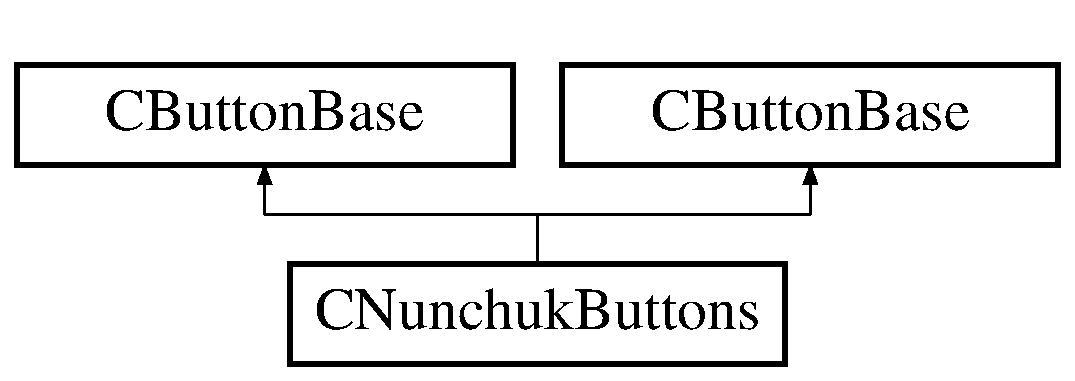
\includegraphics[height=2.000000cm]{class_c_nunchuk_buttons}
\end{center}
\end{figure}
\subsection*{\-Public \-Types}
\begin{DoxyCompactItemize}
\item 
enum {\bfseries \-Button\-Defs} \{ {\bfseries \-B\-U\-T\-T\-O\-N\-\_\-\-Z} =  \-N\-U\-N\-C\-H\-U\-K\-\_\-\-B\-U\-T\-T\-O\-N\-\_\-\-Z, 
{\bfseries \-B\-U\-T\-T\-O\-N\-\_\-\-C} =  \-N\-U\-N\-C\-H\-U\-K\-\_\-\-B\-U\-T\-T\-O\-N\-\_\-\-C, 
{\bfseries \-B\-U\-T\-T\-O\-N\-\_\-\-A\-L\-L} =  \-N\-U\-N\-C\-H\-U\-K\-\_\-\-B\-U\-T\-T\-O\-N\-\_\-\-A\-L\-L
 \}
\end{DoxyCompactItemize}
\subsection*{\-Public \-Member \-Functions}
\begin{DoxyCompactItemize}
\item 
\hypertarget{class_c_nunchuk_buttons_a9ba6eadd235b5078f8d1b751488b7002}{{\bfseries \-C\-Nunchuk\-Buttons} (void $\ast$\-Buttons\-Ptr, void $\ast$\-Buttons\-Held\-Ptr, void $\ast$\-Buttons\-Released\-Ptr)}\label{class_c_nunchuk_buttons_a9ba6eadd235b5078f8d1b751488b7002}

\item 
\hypertarget{class_c_button_base_a0d4758b9e756a8c3c2bb39b907ea9170}{int {\bfseries is\-Pressed} (int \-Button)}\label{class_c_button_base_a0d4758b9e756a8c3c2bb39b907ea9170}

\item 
\hypertarget{class_c_button_base_a67e38daead9d22e33f6a3d85902d1f98}{int {\bfseries is\-Held} (int \-Button)}\label{class_c_button_base_a67e38daead9d22e33f6a3d85902d1f98}

\item 
\hypertarget{class_c_button_base_a575dee487bcca1abf29c1084dfdd5bb8}{int {\bfseries is\-Released} (int \-Button)}\label{class_c_button_base_a575dee487bcca1abf29c1084dfdd5bb8}

\item 
\hypertarget{class_c_button_base_ab74fd21217c5e379a613b7474af4f9b8}{int {\bfseries is\-Just\-Pressed} (int \-Button)}\label{class_c_button_base_ab74fd21217c5e379a613b7474af4f9b8}

\end{DoxyCompactItemize}
\subsection*{\-Private \-Member \-Functions}
\begin{DoxyCompactItemize}
\item 
\hypertarget{class_c_nunchuk_buttons_a1fa701dac6b81d6bf8da7ed3b88ac0a1}{short {\bfseries \-Cast} (void $\ast$\-Ptr)}\label{class_c_nunchuk_buttons_a1fa701dac6b81d6bf8da7ed3b88ac0a1}

\end{DoxyCompactItemize}


\subsection{\-Detailed \-Description}


\-Definition at line 84 of file wiicpp.\-h.



\-The documentation for this class was generated from the following files\-:\begin{DoxyCompactItemize}
\item 
wiicpp.\-h\item 
wiicpp.\-cpp\end{DoxyCompactItemize}

\hypertarget{class_c_weight_sensor}{\section{C\-Weight\-Sensor Class Reference}
\label{class_c_weight_sensor}\index{C\-Weight\-Sensor@{C\-Weight\-Sensor}}
}
\subsection*{Public Member Functions}
\begin{DoxyCompactItemize}
\item 
\hypertarget{class_c_weight_sensor_a04fea64b48194689bf78171e51e97b2d}{{\bfseries C\-Weight\-Sensor} (struct \hyperlink{structpressure__t}{pressure\-\_\-t} $\ast$Raw\-Weight, struct \hyperlink{structpressure__t}{pressure\-\_\-t} $\ast$Low\-Cal\-Weight, struct \hyperlink{structpressure__t}{pressure\-\_\-t} $\ast$Medium\-Cal\-Weight, struct \hyperlink{structpressure__t}{pressure\-\_\-t} $\ast$High\-Cal\-Weight, struct \hyperlink{structpressure__weight__t}{pressure\-\_\-weight\-\_\-t} $\ast$Weight, struct \hyperlink{structbalance__board__t}{balance\-\_\-board\-\_\-t} $\ast$B\-B\-Ptr)}\label{class_c_weight_sensor_a04fea64b48194689bf78171e51e97b2d}

\item 
\hypertarget{class_c_weight_sensor_a3afa84d9e73a9d4d86462661549b3114}{void {\bfseries Get\-Raw\-Weight} (int \&Top\-Left, int \&Top\-Right, int \&Bottom\-Left, int \&Bottom\-Right)}\label{class_c_weight_sensor_a3afa84d9e73a9d4d86462661549b3114}

\item 
\hypertarget{class_c_weight_sensor_a8c7a1bc975f98685aaad423a1e26cffd}{void {\bfseries Get\-Weight} (float \&Total\-Weight, float \&Top\-Left, float \&Top\-Right, float \&Bottom\-Left, float \&Bottom\-Right)}\label{class_c_weight_sensor_a8c7a1bc975f98685aaad423a1e26cffd}

\item 
\hypertarget{class_c_weight_sensor_a6cf2534f75d4f3dd629d49958f0ba7ee}{void {\bfseries Get\-Low\-Cal\-Weight} (int \&Top\-Left, int \&Top\-Right, int \&Bottom\-Left, int \&Bottom\-Right)}\label{class_c_weight_sensor_a6cf2534f75d4f3dd629d49958f0ba7ee}

\item 
\hypertarget{class_c_weight_sensor_a6d3ab9b23321846eb9bcf8401b02ba4e}{void {\bfseries Get\-Medium\-Cal\-Weight} (int \&Top\-Left, int \&Top\-Right, int \&Bottom\-Left, int \&Bottom\-Right)}\label{class_c_weight_sensor_a6d3ab9b23321846eb9bcf8401b02ba4e}

\item 
\hypertarget{class_c_weight_sensor_a554e7bb937f52a77bdc47f5048ef6c0a}{void {\bfseries Get\-High\-Cal\-Weight} (int \&Top\-Left, int \&Top\-Right, int \&Bottom\-Left, int \&Bottom\-Right)}\label{class_c_weight_sensor_a554e7bb937f52a77bdc47f5048ef6c0a}

\item 
\hypertarget{class_c_weight_sensor_a04fea64b48194689bf78171e51e97b2d}{{\bfseries C\-Weight\-Sensor} (struct \hyperlink{structpressure__t}{pressure\-\_\-t} $\ast$Raw\-Weight, struct \hyperlink{structpressure__t}{pressure\-\_\-t} $\ast$Low\-Cal\-Weight, struct \hyperlink{structpressure__t}{pressure\-\_\-t} $\ast$Medium\-Cal\-Weight, struct \hyperlink{structpressure__t}{pressure\-\_\-t} $\ast$High\-Cal\-Weight, struct \hyperlink{structpressure__weight__t}{pressure\-\_\-weight\-\_\-t} $\ast$Weight, struct \hyperlink{structbalance__board__t}{balance\-\_\-board\-\_\-t} $\ast$B\-B\-Ptr)}\label{class_c_weight_sensor_a04fea64b48194689bf78171e51e97b2d}

\item 
\hypertarget{class_c_weight_sensor_a3afa84d9e73a9d4d86462661549b3114}{void {\bfseries Get\-Raw\-Weight} (int \&Top\-Left, int \&Top\-Right, int \&Bottom\-Left, int \&Bottom\-Right)}\label{class_c_weight_sensor_a3afa84d9e73a9d4d86462661549b3114}

\item 
\hypertarget{class_c_weight_sensor_a8c7a1bc975f98685aaad423a1e26cffd}{void {\bfseries Get\-Weight} (float \&Total\-Weight, float \&Top\-Left, float \&Top\-Right, float \&Bottom\-Left, float \&Bottom\-Right)}\label{class_c_weight_sensor_a8c7a1bc975f98685aaad423a1e26cffd}

\item 
\hypertarget{class_c_weight_sensor_a6cf2534f75d4f3dd629d49958f0ba7ee}{void {\bfseries Get\-Low\-Cal\-Weight} (int \&Top\-Left, int \&Top\-Right, int \&Bottom\-Left, int \&Bottom\-Right)}\label{class_c_weight_sensor_a6cf2534f75d4f3dd629d49958f0ba7ee}

\item 
\hypertarget{class_c_weight_sensor_a6d3ab9b23321846eb9bcf8401b02ba4e}{void {\bfseries Get\-Medium\-Cal\-Weight} (int \&Top\-Left, int \&Top\-Right, int \&Bottom\-Left, int \&Bottom\-Right)}\label{class_c_weight_sensor_a6d3ab9b23321846eb9bcf8401b02ba4e}

\item 
\hypertarget{class_c_weight_sensor_a554e7bb937f52a77bdc47f5048ef6c0a}{void {\bfseries Get\-High\-Cal\-Weight} (int \&Top\-Left, int \&Top\-Right, int \&Bottom\-Left, int \&Bottom\-Right)}\label{class_c_weight_sensor_a554e7bb937f52a77bdc47f5048ef6c0a}

\end{DoxyCompactItemize}
\subsection*{Private Attributes}
\begin{DoxyCompactItemize}
\item 
\hypertarget{class_c_weight_sensor_a51f3f16e4dcf5f14bfad1964370b9646}{struct \hyperlink{structpressure__t}{pressure\-\_\-t} $\ast$ {\bfseries mp\-Raw\-Weight}}\label{class_c_weight_sensor_a51f3f16e4dcf5f14bfad1964370b9646}

\item 
\hypertarget{class_c_weight_sensor_acd522228405fa80a189d65abd50f3fa6}{struct \hyperlink{structpressure__t}{pressure\-\_\-t} $\ast$ {\bfseries mp\-Low\-Cal\-Weight}}\label{class_c_weight_sensor_acd522228405fa80a189d65abd50f3fa6}

\item 
\hypertarget{class_c_weight_sensor_a9e92084c2eb934d967df6363e558275d}{struct \hyperlink{structpressure__t}{pressure\-\_\-t} $\ast$ {\bfseries mp\-Medium\-Cal\-Weight}}\label{class_c_weight_sensor_a9e92084c2eb934d967df6363e558275d}

\item 
\hypertarget{class_c_weight_sensor_afb560c691b854a3a6e31bc51ef264270}{struct \hyperlink{structpressure__t}{pressure\-\_\-t} $\ast$ {\bfseries mp\-High\-Cal\-Weight}}\label{class_c_weight_sensor_afb560c691b854a3a6e31bc51ef264270}

\item 
\hypertarget{class_c_weight_sensor_abbbedbb3333fbb3717815b4b7953cd75}{struct \hyperlink{structpressure__weight__t}{pressure\-\_\-weight\-\_\-t} $\ast$ {\bfseries mp\-Weight}}\label{class_c_weight_sensor_abbbedbb3333fbb3717815b4b7953cd75}

\item 
\hypertarget{class_c_weight_sensor_a803935fde640ea62c7904f8703e2c479}{struct \hyperlink{structbalance__board__t}{balance\-\_\-board\-\_\-t} $\ast$ {\bfseries mp\-B\-B\-Ptr}}\label{class_c_weight_sensor_a803935fde640ea62c7904f8703e2c479}

\end{DoxyCompactItemize}


\subsection{Detailed Description}


Definition at line 219 of file wiic\-\_\-r90/src/wiicpp/wiicpp.\-h.



The documentation for this class was generated from the following files\-:\begin{DoxyCompactItemize}
\item 
wiic\-\_\-r90/src/wiicpp/wiicpp.\-h\item 
wiic\-\_\-v1.\-1/src/wiicpp/wiicpp.\-h\item 
wiic\-\_\-r90/src/wiicpp/wiicpp.\-cpp\item 
wiic\-\_\-v1.\-1/src/wiicpp/wiicpp.\-cpp\end{DoxyCompactItemize}

\hypertarget{class_c_wii}{\section{C\-Wii Class Reference}
\label{class_c_wii}\index{C\-Wii@{C\-Wii}}
}
\subsection*{Public Member Functions}
\begin{DoxyCompactItemize}
\item 
\hypertarget{class_c_wii_af61aa748b5c06d551d2e0ca4254f815d}{{\bfseries C\-Wii} (int Max\-Num\-C\-Wiimotes)}\label{class_c_wii_af61aa748b5c06d551d2e0ca4254f815d}

\item 
\hypertarget{class_c_wii_a0e0000682a9469cabc60b6107631fec8}{int {\bfseries Get\-Num\-Connected\-Wiimotes} ()}\label{class_c_wii_a0e0000682a9469cabc60b6107631fec8}

\item 
\hypertarget{class_c_wii_a1ad5ec6adb3939eb2bda5596fb7d6f4a}{void {\bfseries Refresh\-Wiimotes} ()}\label{class_c_wii_a1ad5ec6adb3939eb2bda5596fb7d6f4a}

\item 
\hypertarget{class_c_wii_aed6eb96fc61d08154aee79852def620c}{\hyperlink{class_c_wiimote}{C\-Wiimote} \& {\bfseries Get\-By\-I\-D} (int I\-D, int Refresh=1)}\label{class_c_wii_aed6eb96fc61d08154aee79852def620c}

\item 
\hypertarget{class_c_wii_a9d3c9500516e13b496f22e1e2a1ca44e}{std\-::vector$<$ \hyperlink{class_c_wiimote}{C\-Wiimote} $>$ \& {\bfseries Get\-Wiimotes} (int Refresh=1)}\label{class_c_wii_a9d3c9500516e13b496f22e1e2a1ca44e}

\item 
\hypertarget{class_c_wii_aee1843485afecca45a788df92a56941f}{int {\bfseries Find} (int timeout)}\label{class_c_wii_aee1843485afecca45a788df92a56941f}

\item 
\hypertarget{class_c_wii_acbf1b4f880bf41293e44679cff430794}{int {\bfseries Load\-Registered\-Wiimotes} ()}\label{class_c_wii_acbf1b4f880bf41293e44679cff430794}

\item 
std\-::vector$<$ \hyperlink{class_c_wiimote}{C\-Wiimote} $>$ \& \hyperlink{class_c_wii_aae588e4b73fc2cfe2a50dcc6d23e695d}{Connect} (bool autoreconnect=false)
\begin{DoxyCompactList}\small\item\em Connects to the found Wii devices. \end{DoxyCompactList}\item 
std\-::vector$<$ \hyperlink{class_c_wiimote}{C\-Wiimote} $>$ \& \hyperlink{class_c_wii_ab6ea1b11c12f707d410bf36fee0b16ed}{Find\-And\-Connect} (int timeout=5, bool rumble\-Ack=true, bool autoreconnect=false)
\begin{DoxyCompactList}\small\item\em Finds up to five devices and automatically connect to all of them. \end{DoxyCompactList}\item 
\hypertarget{class_c_wii_acc7affc0e84327f24bd20ef10930f66e}{int {\bfseries Poll} ()}\label{class_c_wii_acc7affc0e84327f24bd20ef10930f66e}

\item 
\hypertarget{class_c_wii_af61aa748b5c06d551d2e0ca4254f815d}{{\bfseries C\-Wii} (int Max\-Num\-C\-Wiimotes)}\label{class_c_wii_af61aa748b5c06d551d2e0ca4254f815d}

\item 
\hypertarget{class_c_wii_a0e0000682a9469cabc60b6107631fec8}{int {\bfseries Get\-Num\-Connected\-Wiimotes} ()}\label{class_c_wii_a0e0000682a9469cabc60b6107631fec8}

\item 
\hypertarget{class_c_wii_a1ad5ec6adb3939eb2bda5596fb7d6f4a}{void {\bfseries Refresh\-Wiimotes} ()}\label{class_c_wii_a1ad5ec6adb3939eb2bda5596fb7d6f4a}

\item 
\hypertarget{class_c_wii_a1ab41805910976445e88c19f6866c8cb}{\hyperlink{class_c_wiimote}{C\-Wiimote} \& {\bfseries Get\-By\-I\-D} (int I\-D, int Refresh=1)}\label{class_c_wii_a1ab41805910976445e88c19f6866c8cb}

\item 
\hypertarget{class_c_wii_a627e741a6b2694b0e98257777e7ca713}{std\-::vector$<$ \hyperlink{class_c_wiimote}{C\-Wiimote} $>$ \& {\bfseries Get\-Wiimotes} (int Refresh=1)}\label{class_c_wii_a627e741a6b2694b0e98257777e7ca713}

\item 
\hypertarget{class_c_wii_aee1843485afecca45a788df92a56941f}{int {\bfseries Find} (int timeout)}\label{class_c_wii_aee1843485afecca45a788df92a56941f}

\item 
\hypertarget{class_c_wii_acbf1b4f880bf41293e44679cff430794}{int {\bfseries Load\-Registered\-Wiimotes} ()}\label{class_c_wii_acbf1b4f880bf41293e44679cff430794}

\item 
\hypertarget{class_c_wii_ae578c5d26fa4f73d51202a2f74dc63bd}{std\-::vector$<$ \hyperlink{class_c_wiimote}{C\-Wiimote} $>$ \& {\bfseries Connect} ()}\label{class_c_wii_ae578c5d26fa4f73d51202a2f74dc63bd}

\item 
\hypertarget{class_c_wii_acc7affc0e84327f24bd20ef10930f66e}{int {\bfseries Poll} ()}\label{class_c_wii_acc7affc0e84327f24bd20ef10930f66e}

\end{DoxyCompactItemize}
\subsection*{Private Attributes}
\begin{DoxyCompactItemize}
\item 
\hypertarget{class_c_wii_a08ce4f60b4808c374b346879188c600d}{struct \hyperlink{structwiimote__t}{wiimote\-\_\-t} $\ast$$\ast$ {\bfseries mp\-Wiimote\-Array}}\label{class_c_wii_a08ce4f60b4808c374b346879188c600d}

\item 
\hypertarget{class_c_wii_ac1979ba03a5d6d4cb90392184bdb083d}{int {\bfseries mp\-Wiimote\-Array\-Size}}\label{class_c_wii_ac1979ba03a5d6d4cb90392184bdb083d}

\item 
\hypertarget{class_c_wii_a85b0f08105957629502c8e932b4d0b1c}{std\-::vector$<$ \hyperlink{class_c_wiimote}{C\-Wiimote} $>$ {\bfseries mp\-Wiimotes\-Vector}}\label{class_c_wii_a85b0f08105957629502c8e932b4d0b1c}

\end{DoxyCompactItemize}


\subsection{Detailed Description}


Definition at line 531 of file wiic\-\_\-r90/src/wiicpp/wiicpp.\-h.



\subsection{Member Function Documentation}
\hypertarget{class_c_wii_aae588e4b73fc2cfe2a50dcc6d23e695d}{\index{C\-Wii@{C\-Wii}!Connect@{Connect}}
\index{Connect@{Connect}!CWii@{C\-Wii}}
\subsubsection[{Connect}]{\setlength{\rightskip}{0pt plus 5cm}std\-::vector$<$ {\bf C\-Wiimote} $>$ \& C\-Wii\-::\-Connect (
\begin{DoxyParamCaption}
\item[{bool}]{autoreconnect = {\ttfamily false}}
\end{DoxyParamCaption}
)}}\label{class_c_wii_aae588e4b73fc2cfe2a50dcc6d23e695d}


Connects to the found Wii devices. 


\begin{DoxyParams}{Parameters}
{\em autoreconnect} & \mbox{[}in\mbox{]} Automatically attempt to re-\/connect a Wii device in case of unexpected disconnection (default is disabled) \\
\hline
\end{DoxyParams}


Definition at line 928 of file wiic\-\_\-r90/src/wiicpp/wiicpp.\-cpp.

\hypertarget{class_c_wii_ab6ea1b11c12f707d410bf36fee0b16ed}{\index{C\-Wii@{C\-Wii}!Find\-And\-Connect@{Find\-And\-Connect}}
\index{Find\-And\-Connect@{Find\-And\-Connect}!CWii@{C\-Wii}}
\subsubsection[{Find\-And\-Connect}]{\setlength{\rightskip}{0pt plus 5cm}std\-::vector$<$ {\bf C\-Wiimote} $>$ \& C\-Wii\-::\-Find\-And\-Connect (
\begin{DoxyParamCaption}
\item[{int}]{timeout = {\ttfamily 5}, }
\item[{bool}]{rumble\-Ack = {\ttfamily true}, }
\item[{bool}]{autoreconnect = {\ttfamily false}}
\end{DoxyParamCaption}
)}}\label{class_c_wii_ab6ea1b11c12f707d410bf36fee0b16ed}


Finds up to five devices and automatically connect to all of them. 


\begin{DoxyParams}{Parameters}
{\em timeout} & \mbox{[}in\mbox{]} Timeout for the discovery step (default is 5 seconds) \\
\hline
{\em rumble\-Ack} & \mbox{[}in\mbox{]} Each found and connected device will receive a small rumble ack (deafult is enabled) \\
\hline
{\em autoreconnect} & \mbox{[}in\mbox{]} Automatically attempt to re-\/connect a Wii device in case of unexpected disconnection (default is disabled) \\
\hline
\end{DoxyParams}


Definition at line 954 of file wiic\-\_\-r90/src/wiicpp/wiicpp.\-cpp.



The documentation for this class was generated from the following files\-:\begin{DoxyCompactItemize}
\item 
wiic\-\_\-r90/src/wiicpp/wiicpp.\-h\item 
wiic\-\_\-v1.\-1/src/wiicpp/wiicpp.\-h\item 
wiic\-\_\-r90/src/wiicpp/wiicpp.\-cpp\item 
wiic\-\_\-v1.\-1/src/wiicpp/wiicpp.\-cpp\end{DoxyCompactItemize}

\hypertarget{class_c_wiimote}{\section{\-C\-Wiimote \-Class \-Reference}
\label{class_c_wiimote}\index{\-C\-Wiimote@{\-C\-Wiimote}}
}
\subsection*{\-Public \-Types}
\begin{DoxyCompactItemize}
\item 
enum {\bfseries \-L\-E\-D\-S} \{ \*
{\bfseries \-L\-E\-D\-\_\-\-N\-O\-N\-E} =  \-W\-I\-I\-M\-O\-T\-E\-\_\-\-L\-E\-D\-\_\-\-N\-O\-N\-E, 
{\bfseries \-L\-E\-D\-\_\-1} =  \-W\-I\-I\-M\-O\-T\-E\-\_\-\-L\-E\-D\-\_\-1, 
{\bfseries \-L\-E\-D\-\_\-2} =  \-W\-I\-I\-M\-O\-T\-E\-\_\-\-L\-E\-D\-\_\-2, 
{\bfseries \-L\-E\-D\-\_\-3} =  \-W\-I\-I\-M\-O\-T\-E\-\_\-\-L\-E\-D\-\_\-3, 
\*
{\bfseries \-L\-E\-D\-\_\-4} =  \-W\-I\-I\-M\-O\-T\-E\-\_\-\-L\-E\-D\-\_\-4
 \}
\item 
enum {\bfseries \-Flags} \{ {\bfseries \-F\-L\-A\-G\-\_\-\-S\-M\-O\-O\-T\-H\-I\-N\-G} =  \-W\-I\-I\-C\-\_\-\-S\-M\-O\-O\-T\-H\-I\-N\-G, 
{\bfseries \-F\-L\-A\-G\-\_\-\-C\-O\-N\-T\-I\-N\-U\-O\-U\-S} =  \-W\-I\-I\-C\-\_\-\-C\-O\-N\-T\-I\-N\-U\-O\-U\-S, 
{\bfseries \-F\-L\-A\-G\-\_\-\-O\-R\-I\-E\-N\-T\-\_\-\-T\-H\-R\-E\-S\-H} =  \-W\-I\-I\-C\-\_\-\-O\-R\-I\-E\-N\-T\-\_\-\-T\-H\-R\-E\-S\-H, 
{\bfseries \-F\-L\-A\-G\-\_\-\-I\-N\-I\-T\-\_\-\-F\-L\-A\-G\-S} =  \-W\-I\-I\-C\-\_\-\-I\-N\-I\-T\-\_\-\-F\-L\-A\-G\-S
 \}
\item 
enum {\bfseries \-Event\-Types} \{ \*
{\bfseries \-E\-V\-E\-N\-T\-\_\-\-N\-O\-N\-E} =  \-W\-I\-I\-C\-\_\-\-N\-O\-N\-E, 
{\bfseries \-E\-V\-E\-N\-T\-\_\-\-E\-V\-E\-N\-T} =  \-W\-I\-I\-C\-\_\-\-E\-V\-E\-N\-T, 
{\bfseries \-E\-V\-E\-N\-T\-\_\-\-S\-T\-A\-T\-U\-S} =  \-W\-I\-I\-C\-\_\-\-S\-T\-A\-T\-U\-S, 
{\bfseries \-E\-V\-E\-N\-T\-\_\-\-C\-O\-N\-N\-E\-C\-T} =  \-W\-I\-I\-C\-\_\-\-C\-O\-N\-N\-E\-C\-T, 
\*
{\bfseries \-E\-V\-E\-N\-T\-\_\-\-D\-I\-S\-C\-O\-N\-N\-E\-C\-T} =  \-W\-I\-I\-C\-\_\-\-D\-I\-S\-C\-O\-N\-N\-E\-C\-T, 
{\bfseries \-E\-V\-E\-N\-T\-\_\-\-U\-N\-E\-X\-P\-E\-C\-T\-E\-D\-\_\-\-D\-I\-S\-C\-O\-N\-N\-E\-C\-T} =  \-W\-I\-I\-C\-\_\-\-U\-N\-E\-X\-P\-E\-C\-T\-E\-D\-\_\-\-D\-I\-S\-C\-O\-N\-N\-E\-C\-T, 
{\bfseries \-E\-V\-E\-N\-T\-\_\-\-R\-E\-A\-D\-\_\-\-D\-A\-T\-A} =  \-W\-I\-I\-C\-\_\-\-R\-E\-A\-D\-\_\-\-D\-A\-T\-A, 
{\bfseries \-E\-V\-E\-N\-T\-\_\-\-N\-U\-N\-C\-H\-U\-K\-\_\-\-I\-N\-S\-E\-R\-T\-E\-D} =  \-W\-I\-I\-C\-\_\-\-N\-U\-N\-C\-H\-U\-K\-\_\-\-I\-N\-S\-E\-R\-T\-E\-D, 
\*
{\bfseries \-E\-V\-E\-N\-T\-\_\-\-N\-U\-N\-C\-H\-U\-K\-\_\-\-R\-E\-M\-O\-V\-E\-D} =  \-W\-I\-I\-C\-\_\-\-N\-U\-N\-C\-H\-U\-K\-\_\-\-R\-E\-M\-O\-V\-E\-D, 
{\bfseries \-E\-V\-E\-N\-T\-\_\-\-C\-L\-A\-S\-S\-I\-C\-\_\-\-C\-T\-R\-L\-\_\-\-I\-N\-S\-E\-R\-T\-E\-D} =  \-W\-I\-I\-C\-\_\-\-C\-L\-A\-S\-S\-I\-C\-\_\-\-C\-T\-R\-L\-\_\-\-I\-N\-S\-E\-R\-T\-E\-D, 
{\bfseries \-E\-V\-E\-N\-T\-\_\-\-C\-L\-A\-S\-S\-I\-C\-\_\-\-C\-T\-R\-L\-\_\-\-R\-E\-M\-O\-V\-E\-D} =  \-W\-I\-I\-C\-\_\-\-C\-L\-A\-S\-S\-I\-C\-\_\-\-C\-T\-R\-L\-\_\-\-R\-E\-M\-O\-V\-E\-D, 
{\bfseries \-E\-V\-E\-N\-T\-\_\-\-G\-U\-I\-T\-A\-R\-\_\-\-H\-E\-R\-O\-\_\-3\-\_\-\-C\-T\-R\-L\-\_\-\-I\-N\-S\-E\-R\-T\-E\-D} =  \-W\-I\-I\-C\-\_\-\-G\-U\-I\-T\-A\-R\-\_\-\-H\-E\-R\-O\-\_\-3\-\_\-\-C\-T\-R\-L\-\_\-\-I\-N\-S\-E\-R\-T\-E\-D, 
\*
{\bfseries \-E\-V\-E\-N\-T\-\_\-\-G\-U\-I\-T\-A\-R\-\_\-\-H\-E\-R\-O\-\_\-3\-\_\-\-C\-T\-R\-L\-\_\-\-R\-E\-M\-O\-V\-E\-D} =  \-W\-I\-I\-C\-\_\-\-G\-U\-I\-T\-A\-R\-\_\-\-H\-E\-R\-O\-\_\-3\-\_\-\-C\-T\-R\-L\-\_\-\-R\-E\-M\-O\-V\-E\-D, 
{\bfseries \-E\-V\-E\-N\-T\-\_\-\-M\-O\-T\-I\-O\-N\-\_\-\-P\-L\-U\-S\-\_\-\-I\-N\-S\-E\-R\-T\-E\-D} =  \-W\-I\-I\-C\-\_\-\-M\-O\-T\-I\-O\-N\-\_\-\-P\-L\-U\-S\-\_\-\-I\-N\-S\-E\-R\-T\-E\-D, 
{\bfseries \-E\-V\-E\-N\-T\-\_\-\-M\-O\-T\-I\-O\-N\-\_\-\-P\-L\-U\-S\-\_\-\-R\-E\-M\-O\-V\-E\-D} =  \-W\-I\-I\-C\-\_\-\-M\-O\-T\-I\-O\-N\-\_\-\-P\-L\-U\-S\-\_\-\-R\-E\-M\-O\-V\-E\-D, 
{\bfseries \-E\-V\-E\-N\-T\-\_\-\-B\-A\-L\-A\-N\-C\-E\-\_\-\-B\-O\-A\-R\-D\-\_\-\-I\-N\-S\-E\-R\-T\-E\-D} =  \-W\-I\-I\-C\-\_\-\-B\-A\-L\-A\-N\-C\-E\-\_\-\-B\-O\-A\-R\-D\-\_\-\-I\-N\-S\-E\-R\-T\-E\-D, 
\*
{\bfseries \-E\-V\-E\-N\-T\-\_\-\-B\-A\-L\-A\-N\-C\-E\-\_\-\-B\-O\-A\-R\-D\-\_\-\-R\-E\-M\-O\-V\-E\-D} =  \-W\-I\-I\-C\-\_\-\-B\-A\-L\-A\-N\-C\-E\-\_\-\-B\-O\-A\-R\-D\-\_\-\-R\-E\-M\-O\-V\-E\-D
 \}
\item 
enum {\bfseries \-On\-Off\-Selection} \{ {\bfseries \-O\-F\-F} =  0, 
{\bfseries \-O\-N} =  1
 \}
\end{DoxyCompactItemize}
\subsection*{\-Public \-Member \-Functions}
\begin{DoxyCompactItemize}
\item 
\hypertarget{class_c_wiimote_aea8deb92b4f4c23ff5f619f92f5740bb}{{\bfseries \-C\-Wiimote} (struct \hyperlink{structwiimote__t}{wiimote\-\_\-t} $\ast$wm\-Ptr)}\label{class_c_wiimote_aea8deb92b4f4c23ff5f619f92f5740bb}

\item 
\hypertarget{class_c_wiimote_af907ec89113a3e2ec6f992bb381c6253}{{\bfseries \-C\-Wiimote} (const \hyperlink{class_c_wiimote}{\-C\-Wiimote} \&copyin)}\label{class_c_wiimote_af907ec89113a3e2ec6f992bb381c6253}

\item 
\hypertarget{class_c_wiimote_a39252c75229d1bc9d2acc126304a7ca6}{void {\bfseries \-Disconnected} ()}\label{class_c_wiimote_a39252c75229d1bc9d2acc126304a7ca6}

\item 
\hypertarget{class_c_wiimote_a4945392c6bcfa461bdcc6b8f5ff25ba1}{void {\bfseries \-Set\-Rumble\-Mode} (\-On\-Off\-Selection \-State)}\label{class_c_wiimote_a4945392c6bcfa461bdcc6b8f5ff25ba1}

\item 
\hypertarget{class_c_wiimote_af1908b383e4a700c270af461bf1b209d}{void {\bfseries \-Toggle\-Rumble} ()}\label{class_c_wiimote_af1908b383e4a700c270af461bf1b209d}

\item 
\hypertarget{class_c_wiimote_a332038d26d6b67d6a566cc1789bae118}{bool {\bfseries is\-Rumble\-Enabled} ()}\label{class_c_wiimote_a332038d26d6b67d6a566cc1789bae118}

\item 
\hypertarget{class_c_wiimote_a288872e2efc61d986b4b49e4b868460b}{int {\bfseries \-Get\-L\-E\-Ds} ()}\label{class_c_wiimote_a288872e2efc61d986b4b49e4b868460b}

\item 
\hypertarget{class_c_wiimote_a3526e61d6a51b6fc8406aeca60e92318}{void {\bfseries \-Set\-L\-E\-Ds} (int \-L\-E\-Ds)}\label{class_c_wiimote_a3526e61d6a51b6fc8406aeca60e92318}

\item 
\hypertarget{class_c_wiimote_adb0acbb6196d8782790e818b4babfde7}{float {\bfseries \-Get\-Battery\-Level} ()}\label{class_c_wiimote_adb0acbb6196d8782790e818b4babfde7}

\item 
\hypertarget{class_c_wiimote_a35a74550a3ec0115ccb39054da4b5064}{int {\bfseries \-Get\-Handshake\-State} ()}\label{class_c_wiimote_a35a74550a3ec0115ccb39054da4b5064}

\item 
\hypertarget{class_c_wiimote_a2f453ed8f5f825d0e503f6f0980d3c70}{\-Event\-Types {\bfseries \-Get\-Event} ()}\label{class_c_wiimote_a2f453ed8f5f825d0e503f6f0980d3c70}

\item 
\hypertarget{class_c_wiimote_a4ed15cfe1340119e090bd9c1feb86e17}{const unsigned char $\ast$ {\bfseries \-Get\-Event\-Buffer} ()}\label{class_c_wiimote_a4ed15cfe1340119e090bd9c1feb86e17}

\item 
\hypertarget{class_c_wiimote_a5f2218caddda3453cfdce8c27262a533}{void {\bfseries \-Set\-Smoothing} (bool \-Smooth)}\label{class_c_wiimote_a5f2218caddda3453cfdce8c27262a533}

\item 
\hypertarget{class_c_wiimote_a3c8c97c0b796d449e143a1a9147925bc}{void {\bfseries \-Set\-Motion\-Sensing\-Mode} (\-On\-Off\-Selection \-State)}\label{class_c_wiimote_a3c8c97c0b796d449e143a1a9147925bc}

\item 
\hypertarget{class_c_wiimote_ad3e4373c9ab443498f7f6b5cb9c73f20}{void {\bfseries \-Enable\-Motion\-Plus} (\-On\-Off\-Selection \-State)}\label{class_c_wiimote_ad3e4373c9ab443498f7f6b5cb9c73f20}

\item 
\hypertarget{class_c_wiimote_ab6d3946204a8836f800e4fd7a7643572}{void {\bfseries \-Log\-Start} (int type=\-W\-I\-I\-C\-\_\-\-L\-O\-G\-\_\-\-N\-O\-N\-E, const string \&file=\char`\"{}\char`\"{})}\label{class_c_wiimote_ab6d3946204a8836f800e4fd7a7643572}

\item 
\hypertarget{class_c_wiimote_ab4ca7dc470ba7da2ae2c321788ac12a6}{void {\bfseries \-Log\-Stop} ()}\label{class_c_wiimote_ab4ca7dc470ba7da2ae2c321788ac12a6}

\item 
\hypertarget{class_c_wiimote_ac07a724c6f0485927c666116d39e6dcc}{void {\bfseries \-Log} ()}\label{class_c_wiimote_ac07a724c6f0485927c666116d39e6dcc}

\item 
\hypertarget{class_c_wiimote_ac3f59a474bed928f29c7ea37a267a516}{struct timeval {\bfseries \-Get\-Timestamp} () const }\label{class_c_wiimote_ac3f59a474bed928f29c7ea37a267a516}

\item 
\hypertarget{class_c_wiimote_af1a936c6f362670eea3663dd15219bd8}{void {\bfseries \-Enable\-Speaker} (\-On\-Off\-Selection \-State)}\label{class_c_wiimote_af1a936c6f362670eea3663dd15219bd8}

\item 
\hypertarget{class_c_wiimote_aab77d7cd365cea3a7d1e8bdbff07de38}{void {\bfseries \-Mute\-Speaker} (\-On\-Off\-Selection \-State)}\label{class_c_wiimote_aab77d7cd365cea3a7d1e8bdbff07de38}

\item 
\hypertarget{class_c_wiimote_a80afecda83601b7e3b33087500b05c84}{void {\bfseries \-Play\-Sound} ()}\label{class_c_wiimote_a80afecda83601b7e3b33087500b05c84}

\item 
\hypertarget{class_c_wiimote_a2894de3f305f27ec1f47d896659a8037}{void {\bfseries \-Read\-Data} (unsigned char $\ast$\-Buffer, unsigned int \-Offset, unsigned int \-Length)}\label{class_c_wiimote_a2894de3f305f27ec1f47d896659a8037}

\item 
\hypertarget{class_c_wiimote_a048e1a9f0612b58b6201ab0f88c7df6c}{void {\bfseries \-Write\-Data} (unsigned int \-Address, unsigned char $\ast$\-Data, unsigned int \-Length)}\label{class_c_wiimote_a048e1a9f0612b58b6201ab0f88c7df6c}

\item 
\hypertarget{class_c_wiimote_aa175e0730a9e68334c010119a280720d}{void {\bfseries \-Update\-Status} ()}\label{class_c_wiimote_aa175e0730a9e68334c010119a280720d}

\item 
\hypertarget{class_c_wiimote_aff65f1d90f0fd1a989f0566385276eeb}{int {\bfseries \-Get\-I\-D} ()}\label{class_c_wiimote_aff65f1d90f0fd1a989f0566385276eeb}

\item 
\hypertarget{class_c_wiimote_a0df092c0ad66746f24793a088ff46e6a}{const char $\ast$ {\bfseries \-Get\-Address} ()}\label{class_c_wiimote_a0df092c0ad66746f24793a088ff46e6a}

\item 
\hypertarget{class_c_wiimote_a0b4b626beab4475fa349de8943c7b24f}{int {\bfseries \-Get\-State} ()}\label{class_c_wiimote_a0b4b626beab4475fa349de8943c7b24f}

\item 
\hypertarget{class_c_wiimote_a2900db59b2eb728f9db885ec1c9aa5e4}{int {\bfseries \-Get\-Flags} ()}\label{class_c_wiimote_a2900db59b2eb728f9db885ec1c9aa5e4}

\item 
\hypertarget{class_c_wiimote_a4efceeac77af5f1e8ca1418841b000b6}{int {\bfseries \-Set\-Flags} (int \-Enable, int \-Disable)}\label{class_c_wiimote_a4efceeac77af5f1e8ca1418841b000b6}

\item 
\hypertarget{class_c_wiimote_a26cd4594fecee2158f4c11a079cad904}{void {\bfseries \-Resync} ()}\label{class_c_wiimote_a26cd4594fecee2158f4c11a079cad904}

\item 
\hypertarget{class_c_wiimote_ad20d26c4cbf0d9b0e4ca26a5d9efed29}{void {\bfseries \-Disconnect} ()}\label{class_c_wiimote_ad20d26c4cbf0d9b0e4ca26a5d9efed29}

\item 
\hypertarget{class_c_wiimote_a25de8c4f00761781102b8fe47227d756}{int {\bfseries is\-Using\-A\-C\-C} ()}\label{class_c_wiimote_a25de8c4f00761781102b8fe47227d756}

\item 
\hypertarget{class_c_wiimote_a1b286b312e419b6181910abc98f44e0d}{int {\bfseries is\-Using\-E\-X\-P} ()}\label{class_c_wiimote_a1b286b312e419b6181910abc98f44e0d}

\item 
\hypertarget{class_c_wiimote_a21eba355433ba66dc42f6b8295ac2f74}{int {\bfseries is\-Using\-I\-R} ()}\label{class_c_wiimote_a21eba355433ba66dc42f6b8295ac2f74}

\item 
\hypertarget{class_c_wiimote_a7427d9d78869c5b3c7deaa25a0f61a3e}{int {\bfseries is\-Using\-Speaker} ()}\label{class_c_wiimote_a7427d9d78869c5b3c7deaa25a0f61a3e}

\item 
\hypertarget{class_c_wiimote_abf98cf75df5eb68d878ea6abe5eea726}{int {\bfseries is\-Speaker\-Muted} ()}\label{class_c_wiimote_abf98cf75df5eb68d878ea6abe5eea726}

\item 
\hypertarget{class_c_wiimote_a8549efa36985e03294333def36878516}{int {\bfseries is\-Using\-Motion\-Plus} ()}\label{class_c_wiimote_a8549efa36985e03294333def36878516}

\item 
\hypertarget{class_c_wiimote_a66043d17813c93bc528ae05e0cc4b8d1}{int {\bfseries is\-L\-E\-D\-Set} (int \-L\-E\-D\-Num)}\label{class_c_wiimote_a66043d17813c93bc528ae05e0cc4b8d1}

\item 
\hypertarget{class_c_wiimote_a085bede0ce129ef6a5c2bb087b66ba71}{bool {\bfseries is\-Log\-Enabled} ()}\label{class_c_wiimote_a085bede0ce129ef6a5c2bb087b66ba71}

\end{DoxyCompactItemize}
\subsection*{\-Public \-Attributes}
\begin{DoxyCompactItemize}
\item 
\hypertarget{class_c_wiimote_adfac321e1529a387b92f485cc1da29f9}{\hyperlink{class_c_i_r}{\-C\-I\-R} {\bfseries \-I\-R}}\label{class_c_wiimote_adfac321e1529a387b92f485cc1da29f9}

\item 
\hypertarget{class_c_wiimote_a88cb9a84630d5cceae9dc95e36ae557c}{\hyperlink{class_c_buttons}{\-C\-Buttons} {\bfseries \-Buttons}}\label{class_c_wiimote_a88cb9a84630d5cceae9dc95e36ae557c}

\item 
\hypertarget{class_c_wiimote_a4c7a137a16717d034641d2207a6a7bb3}{\hyperlink{class_c_accelerometer}{\-C\-Accelerometer} {\bfseries \-Accelerometer}}\label{class_c_wiimote_a4c7a137a16717d034641d2207a6a7bb3}

\item 
\hypertarget{class_c_wiimote_aee65e07504dfcb032dd17680b1f54b4e}{\hyperlink{class_c_expansion_device}{\-C\-Expansion\-Device} {\bfseries \-Expansion\-Device}}\label{class_c_wiimote_aee65e07504dfcb032dd17680b1f54b4e}

\item 
\hypertarget{class_c_wiimote_a4a5e8cdb604e524ca31cf8bb7019e906}{struct \hyperlink{structwiimote__t}{wiimote\-\_\-t} $\ast$ {\bfseries mp\-Wiimote\-Ptr}}\label{class_c_wiimote_a4a5e8cdb604e524ca31cf8bb7019e906}

\end{DoxyCompactItemize}
\subsection*{\-Static \-Public \-Attributes}
\begin{DoxyCompactItemize}
\item 
\hypertarget{class_c_wiimote_a6f1fb15f31fdbdce4c79454fc710cb52}{static const int {\bfseries \-E\-V\-E\-N\-T\-\_\-\-B\-U\-F\-F\-E\-R\-\_\-\-L\-E\-N\-G\-T\-H} = \-M\-A\-X\-\_\-\-P\-A\-Y\-L\-O\-A\-D}\label{class_c_wiimote_a6f1fb15f31fdbdce4c79454fc710cb52}

\end{DoxyCompactItemize}
\subsection*{\-Private \-Attributes}
\begin{DoxyCompactItemize}
\item 
\hypertarget{class_c_wiimote_aee9de2bf7c6e2d2933b2be46f21f4982}{int {\bfseries mp\-Temp\-Int}}\label{class_c_wiimote_aee9de2bf7c6e2d2933b2be46f21f4982}

\item 
\hypertarget{class_c_wiimote_a2617e6071bfc6712961d6b7edb79c2e5}{float {\bfseries mp\-Temp\-Float}}\label{class_c_wiimote_a2617e6071bfc6712961d6b7edb79c2e5}

\item 
\hypertarget{class_c_wiimote_a211cbf074ff990c86b441c84ad003493}{\hyperlink{class_logger}{\-Logger} {\bfseries logger}}\label{class_c_wiimote_a211cbf074ff990c86b441c84ad003493}

\item 
\hypertarget{class_c_wiimote_a9569ece9c54e7483b1f52a3a94ecc746}{int {\bfseries log\-Type}}\label{class_c_wiimote_a9569ece9c54e7483b1f52a3a94ecc746}

\end{DoxyCompactItemize}


\subsection{\-Detailed \-Description}


\-Definition at line 400 of file wiicpp.\-h.



\-The documentation for this class was generated from the following files\-:\begin{DoxyCompactItemize}
\item 
wiicpp.\-h\item 
wiicpp.\-cpp\end{DoxyCompactItemize}

\hypertarget{class_dataset}{\section{Dataset Class Reference}
\label{class_dataset}\index{Dataset@{Dataset}}
}


A \hyperlink{class_dataset}{Dataset} is a collection of trainings, which can represent multiple gestures acquired over time, with different lenghts, and with different approaches.  




{\ttfamily \#include $<$dataset.\-h$>$}

\subsection*{Public Member Functions}
\begin{DoxyCompactItemize}
\item 
\hypertarget{class_dataset_a2ef0a4a688a218d55ef061c6df659a4a}{\hyperlink{class_dataset_a2ef0a4a688a218d55ef061c6df659a4a}{Dataset} ()}\label{class_dataset_a2ef0a4a688a218d55ef061c6df659a4a}

\begin{DoxyCompactList}\small\item\em Default constructor. \end{DoxyCompactList}\item 
\hyperlink{class_dataset_a299c3198f6325d0c627aa029ed24e2e5}{Dataset} (const string \&filename)
\begin{DoxyCompactList}\small\item\em Creates a \hyperlink{class_dataset}{Dataset} object from a log file. \end{DoxyCompactList}\item 
\hypertarget{class_dataset_a7f38b79ccbf9ada90d68d3a50250b193}{\hyperlink{class_dataset_a7f38b79ccbf9ada90d68d3a50250b193}{$\sim$\-Dataset} ()}\label{class_dataset_a7f38b79ccbf9ada90d68d3a50250b193}

\begin{DoxyCompactList}\small\item\em \hyperlink{class_dataset}{Dataset} destructor, which calls clear. \end{DoxyCompactList}\item 
unsigned int \hyperlink{class_dataset_a389855d6b88c8257041bcbc489759aae}{size} () const 
\begin{DoxyCompactList}\small\item\em Retrieves the dataset's size. \end{DoxyCompactList}\item 
const \hyperlink{class_training}{Training} $\ast$ \hyperlink{class_dataset_af776f6046312827aed048d641e29449b}{training\-At} (const unsigned int i) const 
\begin{DoxyCompactList}\small\item\em Returns a training in the dataset as a constant pointer. \end{DoxyCompactList}\item 
\hyperlink{class_training}{Training} $\ast$ \hyperlink{class_dataset_adf05adb75cc0692104dc809ab030e967}{training\-At} (const unsigned int i)
\begin{DoxyCompactList}\small\item\em Returns a training in the dataset as a pointer. \end{DoxyCompactList}\item 
void \hyperlink{class_dataset_a3dd1b2db5490c75c59b23680bb7b8b53}{add\-Training} (\hyperlink{class_training}{Training} $\ast$training)
\begin{DoxyCompactList}\small\item\em Adds a training to the dataset. \end{DoxyCompactList}\item 
bool \hyperlink{class_dataset_a371d55ca351e5f805d8d5c7ffe51c829}{load\-Dataset} (const string \&filename)
\begin{DoxyCompactList}\small\item\em Loads a new dataset from file, erasing the current one (if not saved on file). \end{DoxyCompactList}\item 
bool \hyperlink{class_dataset_a97193aebac43df3a98852a8a675702ab}{save} (const char $\ast$filename, const char $\ast$addr) const 
\begin{DoxyCompactList}\small\item\em Saves the current dataset in a file. \end{DoxyCompactList}\item 
void \hyperlink{class_dataset_a67744c3bdc87acd2a8189b9c4fbcd192}{clear} ()
\begin{DoxyCompactList}\small\item\em Deallocates and deletes all the current trainings in the dataset. \end{DoxyCompactList}\item 
bool \hyperlink{class_dataset_a51c528f515d44baee36589e8de11af50}{is\-Valid} () const 
\begin{DoxyCompactList}\small\item\em Checks if the instance has a valid dataset loaded. \end{DoxyCompactList}\end{DoxyCompactItemize}
\subsection*{Protected Member Functions}
\begin{DoxyCompactItemize}
\item 
void \hyperlink{class_dataset_a23110f7d2b6bc77a388e8dafee9772b3}{save\-Header} (ofstream \&out, const char $\ast$addr) const 
\begin{DoxyCompactList}\small\item\em Saves the initial header of Wii\-C's log files. \end{DoxyCompactList}\end{DoxyCompactItemize}
\subsection*{Private Attributes}
\begin{DoxyCompactItemize}
\item 
\hypertarget{class_dataset_a4491c33243fb10969489cc4c3e25de02}{vector$<$ \hyperlink{class_training}{Training} $\ast$ $>$ {\bfseries trainings}}\label{class_dataset_a4491c33243fb10969489cc4c3e25de02}

\item 
\hypertarget{class_dataset_a55ac9c41a1f3a2bc08ca053df147d163}{bool {\bfseries loaded}}\label{class_dataset_a55ac9c41a1f3a2bc08ca053df147d163}

\end{DoxyCompactItemize}


\subsection{Detailed Description}
A \hyperlink{class_dataset}{Dataset} is a collection of trainings, which can represent multiple gestures acquired over time, with different lenghts, and with different approaches. 

Definition at line 15 of file dataset.\-h.



\subsection{Constructor \& Destructor Documentation}
\hypertarget{class_dataset_a299c3198f6325d0c627aa029ed24e2e5}{\index{Dataset@{Dataset}!Dataset@{Dataset}}
\index{Dataset@{Dataset}!Dataset@{Dataset}}
\subsubsection[{Dataset}]{\setlength{\rightskip}{0pt plus 5cm}Dataset\-::\-Dataset (
\begin{DoxyParamCaption}
\item[{const string \&}]{filename}
\end{DoxyParamCaption}
)\hspace{0.3cm}{\ttfamily [inline]}}}\label{class_dataset_a299c3198f6325d0c627aa029ed24e2e5}


Creates a \hyperlink{class_dataset}{Dataset} object from a log file. 


\begin{DoxyParams}{Parameters}
{\em filename} & Pathname of the dataset to load \\
\hline
\end{DoxyParams}


Definition at line 28 of file dataset.\-h.



\subsection{Member Function Documentation}
\hypertarget{class_dataset_a3dd1b2db5490c75c59b23680bb7b8b53}{\index{Dataset@{Dataset}!add\-Training@{add\-Training}}
\index{add\-Training@{add\-Training}!Dataset@{Dataset}}
\subsubsection[{add\-Training}]{\setlength{\rightskip}{0pt plus 5cm}void Dataset\-::add\-Training (
\begin{DoxyParamCaption}
\item[{{\bf Training} $\ast$}]{t}
\end{DoxyParamCaption}
)}}\label{class_dataset_a3dd1b2db5490c75c59b23680bb7b8b53}


Adds a training to the dataset. 

Add a new training to the dataset.

The new element will be indexed as the last element and will not be copied. It will be responsability of the destructor of the class \hyperlink{class_dataset}{Dataset} to deallocate this element.


\begin{DoxyParams}[1]{Parameters}
\mbox{\tt in}  & {\em training} & The training to add\\
\hline
 & {\em training} & Add a training to the dataset. \\
\hline
\end{DoxyParams}


Definition at line 17 of file dataset.\-cpp.

\hypertarget{class_dataset_a67744c3bdc87acd2a8189b9c4fbcd192}{\index{Dataset@{Dataset}!clear@{clear}}
\index{clear@{clear}!Dataset@{Dataset}}
\subsubsection[{clear}]{\setlength{\rightskip}{0pt plus 5cm}void Dataset\-::clear (
\begin{DoxyParamCaption}
{}
\end{DoxyParamCaption}
)}}\label{class_dataset_a67744c3bdc87acd2a8189b9c4fbcd192}


Deallocates and deletes all the current trainings in the dataset. 

Delete all trainings and clear the buffer.

This method will take care of freeing the memory of each training in the dataset, hence you don't need to free them in your code. 

Definition at line 87 of file dataset.\-cpp.

\hypertarget{class_dataset_a51c528f515d44baee36589e8de11af50}{\index{Dataset@{Dataset}!is\-Valid@{is\-Valid}}
\index{is\-Valid@{is\-Valid}!Dataset@{Dataset}}
\subsubsection[{is\-Valid}]{\setlength{\rightskip}{0pt plus 5cm}bool Dataset\-::is\-Valid (
\begin{DoxyParamCaption}
{}
\end{DoxyParamCaption}
) const\hspace{0.3cm}{\ttfamily [inline]}}}\label{class_dataset_a51c528f515d44baee36589e8de11af50}


Checks if the instance has a valid dataset loaded. 

\begin{DoxyReturn}{Returns}
T\-R\-U\-E if a dataset is correctly loaded, F\-A\-L\-S\-E otherwise 
\end{DoxyReturn}


Definition at line 104 of file dataset.\-h.

\hypertarget{class_dataset_a371d55ca351e5f805d8d5c7ffe51c829}{\index{Dataset@{Dataset}!load\-Dataset@{load\-Dataset}}
\index{load\-Dataset@{load\-Dataset}!Dataset@{Dataset}}
\subsubsection[{load\-Dataset}]{\setlength{\rightskip}{0pt plus 5cm}bool Dataset\-::load\-Dataset (
\begin{DoxyParamCaption}
\item[{const string \&}]{nomefile}
\end{DoxyParamCaption}
)}}\label{class_dataset_a371d55ca351e5f805d8d5c7ffe51c829}


Loads a new dataset from file, erasing the current one (if not saved on file). 

Load a dataset stored in a file.


\begin{DoxyParams}[1]{Parameters}
\mbox{\tt in}  & {\em filename} & Filename of the dataset to load\\
\hline
 & {\em filename} & \hyperlink{class_dataset}{Dataset} filename \\
\hline
\end{DoxyParams}


Definition at line 30 of file dataset.\-cpp.

\hypertarget{class_dataset_a97193aebac43df3a98852a8a675702ab}{\index{Dataset@{Dataset}!save@{save}}
\index{save@{save}!Dataset@{Dataset}}
\subsubsection[{save}]{\setlength{\rightskip}{0pt plus 5cm}bool Dataset\-::save (
\begin{DoxyParamCaption}
\item[{const char $\ast$}]{file, }
\item[{const char $\ast$}]{addr}
\end{DoxyParamCaption}
) const}}\label{class_dataset_a97193aebac43df3a98852a8a675702ab}


Saves the current dataset in a file. 

Save the dataset into a file for training and recognition.


\begin{DoxyParams}[1]{Parameters}
\mbox{\tt in}  & {\em filename} & Desired filename of the saved dataset \\
\hline
\mbox{\tt in}  & {\em addr} & M\-A\-C address of the source device for the dataset\\
\hline
 & {\em filename} & Pathname of the destination file \\
\hline
 & {\em addr} & Wii device mac address \\
\hline
\end{DoxyParams}


Definition at line 105 of file dataset.\-cpp.

\hypertarget{class_dataset_a23110f7d2b6bc77a388e8dafee9772b3}{\index{Dataset@{Dataset}!save\-Header@{save\-Header}}
\index{save\-Header@{save\-Header}!Dataset@{Dataset}}
\subsubsection[{save\-Header}]{\setlength{\rightskip}{0pt plus 5cm}void Dataset\-::save\-Header (
\begin{DoxyParamCaption}
\item[{ofstream \&}]{out, }
\item[{const char $\ast$}]{addr}
\end{DoxyParamCaption}
) const\hspace{0.3cm}{\ttfamily [protected]}}}\label{class_dataset_a23110f7d2b6bc77a388e8dafee9772b3}


Saves the initial header of Wii\-C's log files. 

Save the dataset header into a file.


\begin{DoxyParams}[1]{Parameters}
\mbox{\tt in}  & {\em out} & The output stream of the log file \\
\hline
\mbox{\tt in}  & {\em addr} & M\-A\-C address of the source device for the dataset\\
\hline
 & {\em out} & Output file stream \\
\hline
 & {\em addr} & Wii device M\-A\-C address \\
\hline
\end{DoxyParams}


Definition at line 135 of file dataset.\-cpp.

\hypertarget{class_dataset_a389855d6b88c8257041bcbc489759aae}{\index{Dataset@{Dataset}!size@{size}}
\index{size@{size}!Dataset@{Dataset}}
\subsubsection[{size}]{\setlength{\rightskip}{0pt plus 5cm}unsigned int Dataset\-::size (
\begin{DoxyParamCaption}
{}
\end{DoxyParamCaption}
) const\hspace{0.3cm}{\ttfamily [inline]}}}\label{class_dataset_a389855d6b88c8257041bcbc489759aae}


Retrieves the dataset's size. 

\begin{DoxyReturn}{Returns}
the number of trainings collected in the current dataset 
\end{DoxyReturn}


Definition at line 36 of file dataset.\-h.

\hypertarget{class_dataset_af776f6046312827aed048d641e29449b}{\index{Dataset@{Dataset}!training\-At@{training\-At}}
\index{training\-At@{training\-At}!Dataset@{Dataset}}
\subsubsection[{training\-At}]{\setlength{\rightskip}{0pt plus 5cm}const {\bf Training}$\ast$ Dataset\-::training\-At (
\begin{DoxyParamCaption}
\item[{const unsigned int}]{i}
\end{DoxyParamCaption}
) const\hspace{0.3cm}{\ttfamily [inline]}}}\label{class_dataset_af776f6046312827aed048d641e29449b}


Returns a training in the dataset as a constant pointer. 


\begin{DoxyParams}[1]{Parameters}
\mbox{\tt in}  & {\em i} & The training index in the dataset\\
\hline
\end{DoxyParams}
\begin{DoxyReturn}{Returns}
A constant pointer to the \hyperlink{class_training}{Training} object corresponding to the i-\/th element in the dataset 
\end{DoxyReturn}


Definition at line 45 of file dataset.\-h.

\hypertarget{class_dataset_adf05adb75cc0692104dc809ab030e967}{\index{Dataset@{Dataset}!training\-At@{training\-At}}
\index{training\-At@{training\-At}!Dataset@{Dataset}}
\subsubsection[{training\-At}]{\setlength{\rightskip}{0pt plus 5cm}{\bf Training}$\ast$ Dataset\-::training\-At (
\begin{DoxyParamCaption}
\item[{const unsigned int}]{i}
\end{DoxyParamCaption}
)\hspace{0.3cm}{\ttfamily [inline]}}}\label{class_dataset_adf05adb75cc0692104dc809ab030e967}


Returns a training in the dataset as a pointer. 


\begin{DoxyParams}[1]{Parameters}
\mbox{\tt in}  & {\em i} & The training index in the dataset\\
\hline
\end{DoxyParams}
\begin{DoxyReturn}{Returns}
A pointer to the \hyperlink{class_training}{Training} object corresponding to the i-\/th element in the dataset 
\end{DoxyReturn}


Definition at line 61 of file dataset.\-h.



The documentation for this class was generated from the following files\-:\begin{DoxyCompactItemize}
\item 
\hyperlink{dataset_8h}{dataset.\-h}\item 
dataset.\-cpp\end{DoxyCompactItemize}

\hypertarget{structexpansion__t}{\section{expansion\-\_\-t Struct Reference}
\label{structexpansion__t}\index{expansion\-\_\-t@{expansion\-\_\-t}}
}


Generic expansion device plugged into wiimote.  




{\ttfamily \#include $<$wiic\-\_\-structs.\-h$>$}

\subsection*{Public Attributes}
\begin{DoxyCompactItemize}
\item 
\hypertarget{structexpansion__t_a6b8f85a1f69582f0d20818b6737bbe1f}{int \hyperlink{structexpansion__t_a6b8f85a1f69582f0d20818b6737bbe1f}{type}}\label{structexpansion__t_a6b8f85a1f69582f0d20818b6737bbe1f}

\begin{DoxyCompactList}\small\item\em type of expansion attached \end{DoxyCompactList}\item 
\hypertarget{structexpansion__t_aaeb76b860c9c702f40f422bae3dd70a1}{\begin{tabbing}
xx\=xx\=xx\=xx\=xx\=xx\=xx\=xx\=xx\=\kill
union \{\\
\>struct \hyperlink{structnunchuk__t}{nunchuk\_t} {\bfseries nunchuk}\\
\>struct \hyperlink{structclassic__ctrl__t}{classic\_ctrl\_t} {\bfseries classic}\\
\>struct \hyperlink{structguitar__hero__3__t}{guitar\_hero\_3\_t} {\bfseries gh3}\\
\>struct \hyperlink{structmotion__plus__t}{motion\_plus\_t} {\bfseries mp}\\
\>struct \hyperlink{structbalance__board__t}{balance\_board\_t} {\bfseries bb}\\
\}; }\label{structexpansion__t_aaeb76b860c9c702f40f422bae3dd70a1}
\\

\end{tabbing}\item 
\hypertarget{structexpansion__t_a8c5d768800a772304061c27618adcb9c}{\begin{tabbing}
xx\=xx\=xx\=xx\=xx\=xx\=xx\=xx\=xx\=\kill
union \{\\
\>struct \hyperlink{structnunchuk__t}{nunchuk\_t} {\bfseries nunchuk}\\
\>struct \hyperlink{structclassic__ctrl__t}{classic\_ctrl\_t} {\bfseries classic}\\
\>struct \hyperlink{structguitar__hero__3__t}{guitar\_hero\_3\_t} {\bfseries gh3}\\
\>struct \hyperlink{structmotion__plus__t}{motion\_plus\_t} {\bfseries mp}\\
\>struct \hyperlink{structbalance__board__t}{balance\_board\_t} {\bfseries bb}\\
\}; }\label{structexpansion__t_a8c5d768800a772304061c27618adcb9c}
\\

\end{tabbing}\end{DoxyCompactItemize}


\subsection{Detailed Description}
Generic expansion device plugged into wiimote. 

Definition at line 352 of file wiic\-\_\-r90/src/wiic/wiic\-\_\-structs.\-h.



The documentation for this struct was generated from the following files\-:\begin{DoxyCompactItemize}
\item 
\hyperlink{wiic__r90_2src_2wiic_2wiic__structs_8h}{wiic\-\_\-r90/src/wiic/wiic\-\_\-structs.\-h}\item 
\hyperlink{wiic__v1_81_2src_2wiic_2wiic__structs_8h}{wiic\-\_\-v1.\-1/src/wiic/wiic\-\_\-structs.\-h}\end{DoxyCompactItemize}

\hypertarget{structgforce__t}{\section{gforce\-\_\-t Struct Reference}
\label{structgforce__t}\index{gforce\-\_\-t@{gforce\-\_\-t}}
}


Gravity force struct.  




{\ttfamily \#include $<$wiic\-\_\-structs.\-h$>$}

\subsection*{Public Attributes}
\begin{DoxyCompactItemize}
\item 
\hypertarget{structgforce__t_a97f8ca8f50cd68fd5c5e9530758c461e}{struct \hyperlink{structvec3f__t}{vec3f\-\_\-t} \hyperlink{structgforce__t_a97f8ca8f50cd68fd5c5e9530758c461e}{vec}}\label{structgforce__t_a97f8ca8f50cd68fd5c5e9530758c461e}

\begin{DoxyCompactList}\small\item\em gforce, this may be smoothed if enabled \end{DoxyCompactList}\item 
\hypertarget{structgforce__t_a51f24cbec42c9cb0027c510eaa7c8f46}{struct \hyperlink{structvec3f__t}{vec3f\-\_\-t} \hyperlink{structgforce__t_a51f24cbec42c9cb0027c510eaa7c8f46}{a\-\_\-vec}}\label{structgforce__t_a51f24cbec42c9cb0027c510eaa7c8f46}

\begin{DoxyCompactList}\small\item\em gforce (unsmoothed) \end{DoxyCompactList}\end{DoxyCompactItemize}


\subsection{Detailed Description}
Gravity force struct. 

Definition at line 137 of file wiic\-\_\-structs.\-h.



The documentation for this struct was generated from the following file\-:\begin{DoxyCompactItemize}
\item 
\hyperlink{wiic__structs_8h}{wiic\-\_\-structs.\-h}\end{DoxyCompactItemize}

\hypertarget{structguitar__hero__3__t}{\section{guitar\-\_\-hero\-\_\-3\-\_\-t \-Struct \-Reference}
\label{structguitar__hero__3__t}\index{guitar\-\_\-hero\-\_\-3\-\_\-t@{guitar\-\_\-hero\-\_\-3\-\_\-t}}
}


\-Guitar \-Hero 3 expansion device.  




{\ttfamily \#include $<$wiic\-\_\-structs.\-h$>$}

\subsection*{\-Public \-Attributes}
\begin{DoxyCompactItemize}
\item 
\hypertarget{structguitar__hero__3__t_a65e19f650d5ce8298707eb63707abd7f}{short \hyperlink{structguitar__hero__3__t_a65e19f650d5ce8298707eb63707abd7f}{btns}}\label{structguitar__hero__3__t_a65e19f650d5ce8298707eb63707abd7f}

\begin{DoxyCompactList}\small\item\em what buttons have just been pressed \end{DoxyCompactList}\item 
\hypertarget{structguitar__hero__3__t_ab738e83c9952dec3145e60a4b97727ce}{short \hyperlink{structguitar__hero__3__t_ab738e83c9952dec3145e60a4b97727ce}{btns\-\_\-held}}\label{structguitar__hero__3__t_ab738e83c9952dec3145e60a4b97727ce}

\begin{DoxyCompactList}\small\item\em what buttons are being held down \end{DoxyCompactList}\item 
\hypertarget{structguitar__hero__3__t_aefddbb47a726fff6b5e124f3f0008716}{short \hyperlink{structguitar__hero__3__t_aefddbb47a726fff6b5e124f3f0008716}{btns\-\_\-released}}\label{structguitar__hero__3__t_aefddbb47a726fff6b5e124f3f0008716}

\begin{DoxyCompactList}\small\item\em what buttons were just released this \end{DoxyCompactList}\item 
\hypertarget{structguitar__hero__3__t_a600aeec0929ee91d57d4685d79876942}{float \hyperlink{structguitar__hero__3__t_a600aeec0929ee91d57d4685d79876942}{whammy\-\_\-bar}}\label{structguitar__hero__3__t_a600aeec0929ee91d57d4685d79876942}

\begin{DoxyCompactList}\small\item\em whammy bar (range 0-\/1) \end{DoxyCompactList}\item 
\hypertarget{structguitar__hero__3__t_ad35940d97c2fedc7776efb225742f651}{struct \hyperlink{structjoystick__t}{joystick\-\_\-t} \hyperlink{structguitar__hero__3__t_ad35940d97c2fedc7776efb225742f651}{js}}\label{structguitar__hero__3__t_ad35940d97c2fedc7776efb225742f651}

\begin{DoxyCompactList}\small\item\em joystick calibration \end{DoxyCompactList}\end{DoxyCompactItemize}


\subsection{\-Detailed \-Description}
\-Guitar \-Hero 3 expansion device. 

\-Definition at line 308 of file wiic\-\_\-structs.\-h.



\-The documentation for this struct was generated from the following file\-:\begin{DoxyCompactItemize}
\item 
\hyperlink{wiic__structs_8h}{wiic\-\_\-structs.\-h}\end{DoxyCompactItemize}

\hypertarget{structgyro__t}{\section{gyro\-\_\-t \-Struct \-Reference}
\label{structgyro__t}\index{gyro\-\_\-t@{gyro\-\_\-t}}
}


\-Gyro struct.  




{\ttfamily \#include $<$wiic\-\_\-structs.\-h$>$}

\subsection*{\-Public \-Attributes}
\begin{DoxyCompactItemize}
\item 
\hypertarget{structgyro__t_a1a2b1fdd479dd7cbd2f70b2a2cd93e0b}{struct \hyperlink{structvec3b__t}{vec3b\-\_\-t} \hyperlink{structgyro__t_a1a2b1fdd479dd7cbd2f70b2a2cd93e0b}{cal\-\_\-zero}}\label{structgyro__t_a1a2b1fdd479dd7cbd2f70b2a2cd93e0b}

\begin{DoxyCompactList}\small\item\em zero calibration \end{DoxyCompactList}\item 
\hypertarget{structgyro__t_a05d652ae9beed165d906573c002c7560}{float \hyperlink{structgyro__t_a05d652ae9beed165d906573c002c7560}{st\-\_\-alpha}}\label{structgyro__t_a05d652ae9beed165d906573c002c7560}

\begin{DoxyCompactList}\small\item\em alpha value for smoothing \mbox{[}0-\/1\mbox{]} \end{DoxyCompactList}\end{DoxyCompactItemize}


\subsection{\-Detailed \-Description}
\-Gyro struct. 

\-For any device with a gyroscope. 

\-Definition at line 157 of file wiic\-\_\-structs.\-h.



\-The documentation for this struct was generated from the following file\-:\begin{DoxyCompactItemize}
\item 
\hyperlink{wiic__structs_8h}{wiic\-\_\-structs.\-h}\end{DoxyCompactItemize}

\hypertarget{class_gyro_sample}{\section{Gyro\-Sample Class Reference}
\label{class_gyro_sample}\index{Gyro\-Sample@{Gyro\-Sample}}
}
Inheritance diagram for Gyro\-Sample\-:\begin{figure}[H]
\begin{center}
\leavevmode
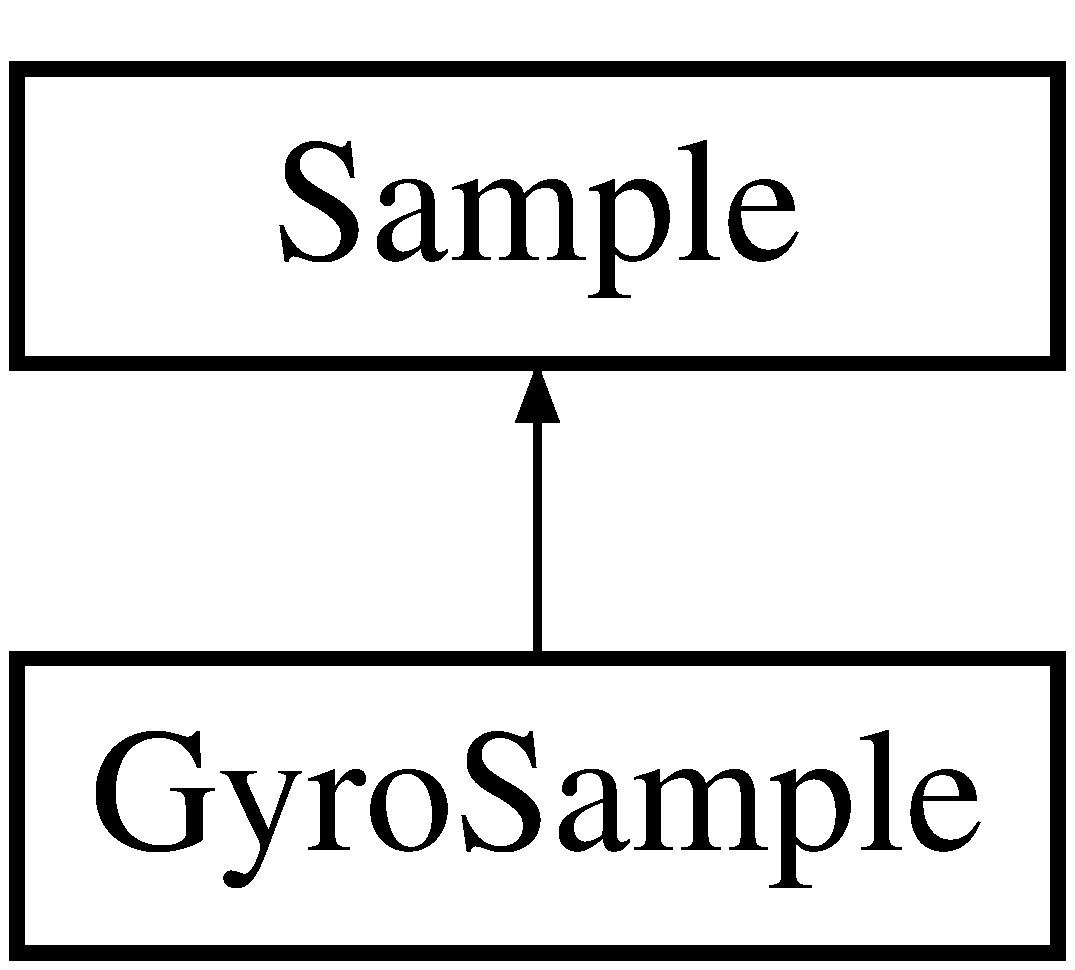
\includegraphics[height=2.000000cm]{class_gyro_sample}
\end{center}
\end{figure}
\subsection*{Public Member Functions}
\begin{DoxyCompactItemize}
\item 
\hypertarget{class_gyro_sample_a5f2b3297cf53498936c2c8fc55b8653b}{{\bfseries Gyro\-Sample} (float r, float p, float y)}\label{class_gyro_sample_a5f2b3297cf53498936c2c8fc55b8653b}

\item 
\hypertarget{class_gyro_sample_ab6010043e58217035a655ccbcf8b3d70}{{\bfseries Gyro\-Sample} (const string \&line)}\label{class_gyro_sample_ab6010043e58217035a655ccbcf8b3d70}

\item 
\hypertarget{class_gyro_sample_a8360f35fbf6fd9e46f25be49f6fc92cd}{float {\bfseries roll} () const }\label{class_gyro_sample_a8360f35fbf6fd9e46f25be49f6fc92cd}

\item 
\hypertarget{class_gyro_sample_a524cde9a9313320cbcf3e9cb6cb4894e}{float {\bfseries pitch} () const }\label{class_gyro_sample_a524cde9a9313320cbcf3e9cb6cb4894e}

\item 
\hypertarget{class_gyro_sample_a6dcbb6633450bff4f6d322c8b4e3ca06}{float {\bfseries yaw} () const }\label{class_gyro_sample_a6dcbb6633450bff4f6d322c8b4e3ca06}

\item 
\hypertarget{class_gyro_sample_a2f8571fe6f29fc4e28ea582ff9f0cfa7}{virtual void {\bfseries save} (ofstream \&out)}\label{class_gyro_sample_a2f8571fe6f29fc4e28ea582ff9f0cfa7}

\item 
\hypertarget{class_sample_ae728243bef5e290d46a2851ea2ce5fe2}{void {\bfseries set\-Log\-Type} (int l)}\label{class_sample_ae728243bef5e290d46a2851ea2ce5fe2}

\item 
\hypertarget{class_sample_aafff0e8223f3eafa001611a63f194c8a}{int {\bfseries get\-Log\-Type} () const }\label{class_sample_aafff0e8223f3eafa001611a63f194c8a}

\item 
\hypertarget{class_sample_a05edd06782fa94517b8daeb29e12057d}{void {\bfseries set\-Timestamp\-From\-Gesture\-Start} (unsigned long t)}\label{class_sample_a05edd06782fa94517b8daeb29e12057d}

\item 
\hypertarget{class_sample_a94a34fe92c0f8a89485042aaea458d94}{unsigned long {\bfseries get\-Timestamp\-From\-Gesture\-Start} () const }\label{class_sample_a94a34fe92c0f8a89485042aaea458d94}

\end{DoxyCompactItemize}
\subsection*{Protected Attributes}
\begin{DoxyCompactItemize}
\item 
\hypertarget{class_sample_a24ea733ab0a815949a57aca2a4740e33}{unsigned long {\bfseries rel\-Timestamp}}\label{class_sample_a24ea733ab0a815949a57aca2a4740e33}

\item 
\hypertarget{class_sample_a3a6454628c790459f41de5c83bf3ec7c}{int {\bfseries log\-Type}}\label{class_sample_a3a6454628c790459f41de5c83bf3ec7c}

\item 
\hypertarget{class_sample_adbde42442423cd9dc8d971bf764391cc}{struct timeval {\bfseries timestamp}}\label{class_sample_adbde42442423cd9dc8d971bf764391cc}

\end{DoxyCompactItemize}
\subsection*{Private Attributes}
\begin{DoxyCompactItemize}
\item 
\hypertarget{class_gyro_sample_a54e5450ba9577976cdaba4f5c2e61422}{float {\bfseries roll\-\_\-}}\label{class_gyro_sample_a54e5450ba9577976cdaba4f5c2e61422}

\item 
\hypertarget{class_gyro_sample_ad2574d31543929b4d54bf64236346bdb}{float {\bfseries pitch\-\_\-}}\label{class_gyro_sample_ad2574d31543929b4d54bf64236346bdb}

\item 
\hypertarget{class_gyro_sample_ae9454e936037dfb739b355e1baed42b5}{float {\bfseries yaw\-\_\-}}\label{class_gyro_sample_ae9454e936037dfb739b355e1baed42b5}

\end{DoxyCompactItemize}


\subsection{Detailed Description}


Definition at line 6 of file gyrosample.\-h.



The documentation for this class was generated from the following files\-:\begin{DoxyCompactItemize}
\item 
gyrosample.\-h\item 
gyrosample.\-cpp\end{DoxyCompactItemize}

\hypertarget{structir__dot__t}{\section{ir\-\_\-dot\-\_\-t Struct Reference}
\label{structir__dot__t}\index{ir\-\_\-dot\-\_\-t@{ir\-\_\-dot\-\_\-t}}
}


A single I\-R source.  




{\ttfamily \#include $<$wiic\-\_\-structs.\-h$>$}

\subsection*{Public Attributes}
\begin{DoxyCompactItemize}
\item 
\hypertarget{structir__dot__t_a80221d94f19596c20184f0fa81e492e7}{\hyperlink{wiic__macros_8h_a0c8186d9b9b7880309c27230bbb5e69d}{byte} \hyperlink{structir__dot__t_a80221d94f19596c20184f0fa81e492e7}{visible}}\label{structir__dot__t_a80221d94f19596c20184f0fa81e492e7}

\begin{DoxyCompactList}\small\item\em if the I\-R source is visible \end{DoxyCompactList}\item 
\hypertarget{structir__dot__t_a34249e77ebf52f4aea5a99e5dcf0b850}{unsigned int \hyperlink{structir__dot__t_a34249e77ebf52f4aea5a99e5dcf0b850}{x}}\label{structir__dot__t_a34249e77ebf52f4aea5a99e5dcf0b850}

\begin{DoxyCompactList}\small\item\em interpolated X coordinate \end{DoxyCompactList}\item 
\hypertarget{structir__dot__t_a09a2a985e3e235e371347bbaf9db30ba}{unsigned int \hyperlink{structir__dot__t_a09a2a985e3e235e371347bbaf9db30ba}{y}}\label{structir__dot__t_a09a2a985e3e235e371347bbaf9db30ba}

\begin{DoxyCompactList}\small\item\em interpolated Y coordinate \end{DoxyCompactList}\item 
\hypertarget{structir__dot__t_a046a0132b74da3c8c334c8e875a763d5}{short \hyperlink{structir__dot__t_a046a0132b74da3c8c334c8e875a763d5}{rx}}\label{structir__dot__t_a046a0132b74da3c8c334c8e875a763d5}

\begin{DoxyCompactList}\small\item\em raw X coordinate (0-\/1023) \end{DoxyCompactList}\item 
\hypertarget{structir__dot__t_ab7fb2aacd27c03155935515907b49065}{short \hyperlink{structir__dot__t_ab7fb2aacd27c03155935515907b49065}{ry}}\label{structir__dot__t_ab7fb2aacd27c03155935515907b49065}

\begin{DoxyCompactList}\small\item\em raw Y coordinate (0-\/767) \end{DoxyCompactList}\item 
\hypertarget{structir__dot__t_a729a0f66a1b6ed5ec6caf999934ef44b}{\hyperlink{wiic__macros_8h_a0c8186d9b9b7880309c27230bbb5e69d}{byte} \hyperlink{structir__dot__t_a729a0f66a1b6ed5ec6caf999934ef44b}{order}}\label{structir__dot__t_a729a0f66a1b6ed5ec6caf999934ef44b}

\begin{DoxyCompactList}\small\item\em increasing order by x-\/axis value \end{DoxyCompactList}\item 
\hypertarget{structir__dot__t_a009422c74d8c2a1dcfe64e669cb7aa91}{\hyperlink{wiic__macros_8h_a0c8186d9b9b7880309c27230bbb5e69d}{byte} \hyperlink{structir__dot__t_a009422c74d8c2a1dcfe64e669cb7aa91}{size}}\label{structir__dot__t_a009422c74d8c2a1dcfe64e669cb7aa91}

\begin{DoxyCompactList}\small\item\em size of the I\-R dot (0-\/15) \end{DoxyCompactList}\end{DoxyCompactItemize}


\subsection{Detailed Description}
A single I\-R source. 

Definition at line 195 of file wiic\-\_\-structs.\-h.



The documentation for this struct was generated from the following file\-:\begin{DoxyCompactItemize}
\item 
\hyperlink{wiic__structs_8h}{wiic\-\_\-structs.\-h}\end{DoxyCompactItemize}

\hypertarget{structir__t}{\section{ir\-\_\-t Struct Reference}
\label{structir__t}\index{ir\-\_\-t@{ir\-\_\-t}}
}


I\-R struct.  




{\ttfamily \#include $<$wiic\-\_\-structs.\-h$>$}

\subsection*{Public Attributes}
\begin{DoxyCompactItemize}
\item 
\hypertarget{structir__t_a77d832ed049dd2edcfdfe05293546d6a}{struct \hyperlink{structir__dot__t}{ir\-\_\-dot\-\_\-t} \hyperlink{structir__t_a77d832ed049dd2edcfdfe05293546d6a}{dot} \mbox{[}4\mbox{]}}\label{structir__t_a77d832ed049dd2edcfdfe05293546d6a}

\begin{DoxyCompactList}\small\item\em I\-R dots. \end{DoxyCompactList}\item 
\hypertarget{structir__t_a406594b90d24e1910ed1a7e02c9aae56}{\hyperlink{wiic__macros_8h_a0c8186d9b9b7880309c27230bbb5e69d}{byte} \hyperlink{structir__t_a406594b90d24e1910ed1a7e02c9aae56}{num\-\_\-dots}}\label{structir__t_a406594b90d24e1910ed1a7e02c9aae56}

\begin{DoxyCompactList}\small\item\em number of dots at this time \end{DoxyCompactList}\item 
\hypertarget{structir__t_a0a54081272fba76534573a4ed8fe9cc9}{enum \hyperlink{wiic__macros_8h_a48b01fa22a869e3fb6afe4b4a4f30658}{aspect\-\_\-t} \hyperlink{structir__t_a0a54081272fba76534573a4ed8fe9cc9}{aspect}}\label{structir__t_a0a54081272fba76534573a4ed8fe9cc9}

\begin{DoxyCompactList}\small\item\em aspect ratio of the screen \end{DoxyCompactList}\item 
\hypertarget{structir__t_a4caa91929b90386e53b9cc7eaa416c8f}{enum ir\-\_\-position\-\_\-t \hyperlink{structir__t_a4caa91929b90386e53b9cc7eaa416c8f}{pos}}\label{structir__t_a4caa91929b90386e53b9cc7eaa416c8f}

\begin{DoxyCompactList}\small\item\em I\-R sensor bar position. \end{DoxyCompactList}\item 
\hypertarget{structir__t_a4aa225245b34b9348af37642a313fbe4}{unsigned int \hyperlink{structir__t_a4aa225245b34b9348af37642a313fbe4}{vres} \mbox{[}2\mbox{]}}\label{structir__t_a4aa225245b34b9348af37642a313fbe4}

\begin{DoxyCompactList}\small\item\em I\-R virtual screen resolution. \end{DoxyCompactList}\item 
\hypertarget{structir__t_acf1668d1cf68dae1918f593af3c08303}{int \hyperlink{structir__t_acf1668d1cf68dae1918f593af3c08303}{offset} \mbox{[}2\mbox{]}}\label{structir__t_acf1668d1cf68dae1918f593af3c08303}

\begin{DoxyCompactList}\small\item\em I\-R X\-Y correction offset. \end{DoxyCompactList}\item 
\hypertarget{structir__t_a04cea1fc7f02e87a35775246e1e34aad}{int \hyperlink{structir__t_a04cea1fc7f02e87a35775246e1e34aad}{state}}\label{structir__t_a04cea1fc7f02e87a35775246e1e34aad}

\begin{DoxyCompactList}\small\item\em keeps track of the I\-R state \end{DoxyCompactList}\item 
\hypertarget{structir__t_affbbd8f9e9bccf428b39f2ac54f797fd}{int \hyperlink{structir__t_affbbd8f9e9bccf428b39f2ac54f797fd}{ax}}\label{structir__t_affbbd8f9e9bccf428b39f2ac54f797fd}

\begin{DoxyCompactList}\small\item\em absolute X coordinate \end{DoxyCompactList}\item 
\hypertarget{structir__t_adad042b5d45b0dd513ceec8f79459750}{int \hyperlink{structir__t_adad042b5d45b0dd513ceec8f79459750}{ay}}\label{structir__t_adad042b5d45b0dd513ceec8f79459750}

\begin{DoxyCompactList}\small\item\em absolute Y coordinate \end{DoxyCompactList}\item 
\hypertarget{structir__t_a1cf171671dfd16626f560b6b1776aeda}{int \hyperlink{structir__t_a1cf171671dfd16626f560b6b1776aeda}{x}}\label{structir__t_a1cf171671dfd16626f560b6b1776aeda}

\begin{DoxyCompactList}\small\item\em calculated X coordinate \end{DoxyCompactList}\item 
\hypertarget{structir__t_aecf2c4663aab868d326caeb7ffd01229}{int \hyperlink{structir__t_aecf2c4663aab868d326caeb7ffd01229}{y}}\label{structir__t_aecf2c4663aab868d326caeb7ffd01229}

\begin{DoxyCompactList}\small\item\em calculated Y coordinate \end{DoxyCompactList}\item 
\hypertarget{structir__t_ae964cb719e73986be124cf190d66d44d}{float \hyperlink{structir__t_ae964cb719e73986be124cf190d66d44d}{distance}}\label{structir__t_ae964cb719e73986be124cf190d66d44d}

\begin{DoxyCompactList}\small\item\em pixel distance between first 2 dots \end{DoxyCompactList}\item 
\hypertarget{structir__t_a94c67dc38b051479b8d786449449c864}{float \hyperlink{structir__t_a94c67dc38b051479b8d786449449c864}{z}}\label{structir__t_a94c67dc38b051479b8d786449449c864}

\begin{DoxyCompactList}\small\item\em calculated distance \end{DoxyCompactList}\end{DoxyCompactItemize}


\subsection{Detailed Description}
I\-R struct. 

Hold all data related to the I\-R tracking. 

Definition at line 214 of file wiic\-\_\-structs.\-h.



The documentation for this struct was generated from the following file\-:\begin{DoxyCompactItemize}
\item 
\hyperlink{wiic__structs_8h}{wiic\-\_\-structs.\-h}\end{DoxyCompactItemize}

\hypertarget{structjoystick__t}{\section{joystick\-\_\-t Struct Reference}
\label{structjoystick__t}\index{joystick\-\_\-t@{joystick\-\_\-t}}
}


Joystick calibration structure.  




{\ttfamily \#include $<$wiic\-\_\-structs.\-h$>$}

\subsection*{Public Attributes}
\begin{DoxyCompactItemize}
\item 
\hypertarget{structjoystick__t_a065529eb4f4ea23be8b95f8705876b12}{struct \hyperlink{structvec2b__t}{vec2b\-\_\-t} \hyperlink{structjoystick__t_a065529eb4f4ea23be8b95f8705876b12}{max}}\label{structjoystick__t_a065529eb4f4ea23be8b95f8705876b12}

\begin{DoxyCompactList}\small\item\em maximum joystick values \end{DoxyCompactList}\item 
\hypertarget{structjoystick__t_aff984e44734968b8f8fdbd52ea8aeb4f}{struct \hyperlink{structvec2b__t}{vec2b\-\_\-t} \hyperlink{structjoystick__t_aff984e44734968b8f8fdbd52ea8aeb4f}{min}}\label{structjoystick__t_aff984e44734968b8f8fdbd52ea8aeb4f}

\begin{DoxyCompactList}\small\item\em minimum joystick values \end{DoxyCompactList}\item 
\hypertarget{structjoystick__t_a7f37b3f10761fd35fe0375377073ac44}{struct \hyperlink{structvec2b__t}{vec2b\-\_\-t} \hyperlink{structjoystick__t_a7f37b3f10761fd35fe0375377073ac44}{center}}\label{structjoystick__t_a7f37b3f10761fd35fe0375377073ac44}

\begin{DoxyCompactList}\small\item\em center joystick values \end{DoxyCompactList}\item 
\hypertarget{structjoystick__t_a59aa4a12fedb3126f21345905d824fc1}{float \hyperlink{structjoystick__t_a59aa4a12fedb3126f21345905d824fc1}{ang}}\label{structjoystick__t_a59aa4a12fedb3126f21345905d824fc1}

\begin{DoxyCompactList}\small\item\em angle the joystick is being held \end{DoxyCompactList}\item 
\hypertarget{structjoystick__t_af358a1cfed3d18c4ce62fb62632b56cf}{float \hyperlink{structjoystick__t_af358a1cfed3d18c4ce62fb62632b56cf}{mag}}\label{structjoystick__t_af358a1cfed3d18c4ce62fb62632b56cf}

\begin{DoxyCompactList}\small\item\em magnitude of the joystick (range 0-\/1) \end{DoxyCompactList}\end{DoxyCompactItemize}


\subsection{Detailed Description}
Joystick calibration structure. 

The angle {\itshape ang} is relative to the positive y-\/axis into quadrant I and ranges from 0 to 360 degrees. So if the joystick is held straight upwards then angle is 0 degrees. If it is held to the right it is 90, down is 180, and left is 270.

The magnitude {\itshape mag} is the distance from the center to where the joystick is being held. The magnitude ranges from 0 to 1. If the joystick is only slightly tilted from the center the magnitude will be low, but if it is closer to the outter edge the value will be higher. 

Definition at line 252 of file wiic\-\_\-structs.\-h.



The documentation for this struct was generated from the following file\-:\begin{DoxyCompactItemize}
\item 
\hyperlink{wiic__structs_8h}{wiic\-\_\-structs.\-h}\end{DoxyCompactItemize}

\hypertarget{class_lights}{\section{\-Lights \-Class \-Reference}
\label{class_lights}\index{\-Lights@{\-Lights}}
}
\subsection*{\-Public \-Member \-Functions}
\begin{DoxyCompactItemize}
\item 
\hypertarget{class_lights_a697efdeb33331a506a1a63a564f5f2e1}{void {\bfseries remove\-Light\-Source} ()}\label{class_lights_a697efdeb33331a506a1a63a564f5f2e1}

\item 
\hypertarget{class_lights_a2b773cfaba5c662fb2a0344be70edc19}{void {\bfseries add\-Light\-Source} ()}\label{class_lights_a2b773cfaba5c662fb2a0344be70edc19}

\item 
\hypertarget{class_lights_a47639f6fd64056f15b9372b80f9ef117}{void {\bfseries init\-\_\-lights} (\-G\-Luint program)}\label{class_lights_a47639f6fd64056f15b9372b80f9ef117}

\end{DoxyCompactItemize}
\subsection*{\-Private \-Attributes}
\begin{DoxyCompactItemize}
\item 
\hypertarget{class_lights_a902e37f0512d3bf9771472fe564bdac1}{vector$<$ \hyperlink{class_light_source}{\-Light\-Source} $>$ {\bfseries the\-Lights}}\label{class_lights_a902e37f0512d3bf9771472fe564bdac1}

\end{DoxyCompactItemize}


\subsection{\-Detailed \-Description}


\-Definition at line 74 of file \-Light\-Source.\-hpp.



\-The documentation for this class was generated from the following file\-:\begin{DoxyCompactItemize}
\item 
\-Light\-Source.\-hpp\end{DoxyCompactItemize}

\hypertarget{class_light_source}{\section{Light\-Source Class Reference}
\label{class_light_source}\index{Light\-Source@{Light\-Source}}
}
\subsection*{Public Member Functions}
\begin{DoxyCompactItemize}
\item 
\hypertarget{class_light_source_a83e373049e705227216bea0ec9774f18}{{\bfseries Light\-Source} (const \hyperlink{struct_angel_1_1vec4}{point4} \&)}\label{class_light_source_a83e373049e705227216bea0ec9774f18}

\item 
\hypertarget{class_light_source_a991346373d3ded70727b07416cd1c04d}{{\bfseries Light\-Source} (const \hyperlink{struct_angel_1_1vec4}{point4} \&, const \hyperlink{struct_angel_1_1vec4}{color4} \&)}\label{class_light_source_a991346373d3ded70727b07416cd1c04d}

\item 
\hypertarget{class_light_source_aec26fce93563c0b1719a211b9b49193f}{{\bfseries Light\-Source} (const \hyperlink{struct_angel_1_1vec4}{point4} \&, const \hyperlink{struct_angel_1_1vec4}{color4} \&, const \hyperlink{struct_angel_1_1vec4}{color4} \&, const \hyperlink{struct_angel_1_1vec4}{color4} \&)}\label{class_light_source_aec26fce93563c0b1719a211b9b49193f}

\item 
\hypertarget{class_light_source_a7ed30701ee0865f8cc60af7de633714b}{{\bfseries Light\-Source} (const \hyperlink{struct_angel_1_1vec4}{point4} \&, const \hyperlink{struct_angel_1_1vec4}{vec4} \&, const \hyperlink{struct_angel_1_1vec4}{color4} \&, const \hyperlink{struct_angel_1_1vec4}{color4} \&, const \hyperlink{struct_angel_1_1vec4}{color4} \&)}\label{class_light_source_a7ed30701ee0865f8cc60af7de633714b}

\item 
\hypertarget{class_light_source_a71dbbd92599046fb93fb1e7740088947}{{\bfseries Light\-Source} (const \hyperlink{class_light_source}{Light\-Source} \&orig)}\label{class_light_source_a71dbbd92599046fb93fb1e7740088947}

\item 
\hypertarget{class_light_source_a5a599502b38a1875ada2579f6c8300ba}{void {\bfseries Set\-Light\-\_\-specular} (\hyperlink{struct_angel_1_1vec4}{color4} \&light\-\_\-specular)}\label{class_light_source_a5a599502b38a1875ada2579f6c8300ba}

\item 
\hypertarget{class_light_source_ab91668c8a2b5e9af25df5e96aef8f930}{\hyperlink{struct_angel_1_1vec4}{color4} {\bfseries Get\-Light\-\_\-specular} () const }\label{class_light_source_ab91668c8a2b5e9af25df5e96aef8f930}

\item 
\hypertarget{class_light_source_a6ecf874ed5a2c0796435a4d7fe7f3d5c}{void {\bfseries Set\-Light\-\_\-diffuse} (\hyperlink{struct_angel_1_1vec4}{color4} \&light\-\_\-diffuse)}\label{class_light_source_a6ecf874ed5a2c0796435a4d7fe7f3d5c}

\item 
\hypertarget{class_light_source_a3b1b4a97762e1cbb51c529166c82f657}{\hyperlink{struct_angel_1_1vec4}{color4} {\bfseries Get\-Light\-\_\-diffuse} () const }\label{class_light_source_a3b1b4a97762e1cbb51c529166c82f657}

\item 
\hypertarget{class_light_source_aabc855fe2998ed9af76c9e3c262d9e5c}{void {\bfseries Set\-Light\-\_\-ambient} (\hyperlink{struct_angel_1_1vec4}{color4} \&light\-\_\-ambient)}\label{class_light_source_aabc855fe2998ed9af76c9e3c262d9e5c}

\item 
\hypertarget{class_light_source_a87b3948456c4d45caa24b7cdd1e02058}{\hyperlink{struct_angel_1_1vec4}{color4} {\bfseries Get\-Light\-\_\-ambient} () const }\label{class_light_source_a87b3948456c4d45caa24b7cdd1e02058}

\item 
\hypertarget{class_light_source_aab4e16f4fabe4fffd9ca614669468b18}{void {\bfseries Set\-Light\-\_\-color} (\hyperlink{struct_angel_1_1vec4}{color4} \&light\-\_\-color)}\label{class_light_source_aab4e16f4fabe4fffd9ca614669468b18}

\item 
\hypertarget{class_light_source_a4e949920966cef628098f5f2199595f2}{\hyperlink{struct_angel_1_1vec4}{color4} {\bfseries Get\-Light\-\_\-color} () const }\label{class_light_source_a4e949920966cef628098f5f2199595f2}

\item 
\hypertarget{class_light_source_aa56fb7f92dffb9640671e3175a2e02d6}{void {\bfseries Set\-Direction} (\hyperlink{struct_angel_1_1vec4}{vec4} \&direction)}\label{class_light_source_aa56fb7f92dffb9640671e3175a2e02d6}

\item 
\hypertarget{class_light_source_a6387fc88c608069ce983a55d88d2bc80}{\hyperlink{struct_angel_1_1vec4}{vec4} {\bfseries Get\-Direction} () const }\label{class_light_source_a6387fc88c608069ce983a55d88d2bc80}

\item 
\hypertarget{class_light_source_a16db60b10fc3490d2940c150e29282e2}{void {\bfseries Set\-Position} (\hyperlink{struct_angel_1_1vec4}{point4} \&z)}\label{class_light_source_a16db60b10fc3490d2940c150e29282e2}

\item 
\hypertarget{class_light_source_a516709d4d71fa7179b006df318ec3ecb}{\hyperlink{struct_angel_1_1vec4}{point4} {\bfseries Get\-Position} () const }\label{class_light_source_a516709d4d71fa7179b006df318ec3ecb}

\item 
\hypertarget{class_light_source_aef1a1468f582bade33af96d96e9d50db}{bool {\bfseries Get\-Complex\-Switch} () const }\label{class_light_source_aef1a1468f582bade33af96d96e9d50db}

\item 
\hypertarget{class_light_source_a8b565d411a56940055ec3f07a401a856}{void {\bfseries Do\-Events} (void)}\label{class_light_source_a8b565d411a56940055ec3f07a401a856}

\item 
\hypertarget{class_light_source_a06c1f646e7d2ca223ab3627c1f713964}{void {\bfseries set\-Effect} (int)}\label{class_light_source_a06c1f646e7d2ca223ab3627c1f713964}

\end{DoxyCompactItemize}
\subsection*{Private Types}
\begin{DoxyCompactItemize}
\item 
enum {\bfseries light\-\_\-effect} \{ \\*
{\bfseries O\-F\-F} = 0, 
{\bfseries O\-N}, 
{\bfseries B\-L\-I\-N\-K}, 
{\bfseries S\-T\-R\-O\-B\-E}, 
\\*
{\bfseries P\-U\-L\-S\-E}
 \}
\end{DoxyCompactItemize}
\subsection*{Private Attributes}
\begin{DoxyCompactItemize}
\item 
\hypertarget{class_light_source_a278ef32fb772d375e03e4c03560502e7}{\hyperlink{struct_angel_1_1vec4}{point4} {\bfseries position}}\label{class_light_source_a278ef32fb772d375e03e4c03560502e7}

\item 
\hypertarget{class_light_source_a104d67d17b33af3a58f2382735afb6c4}{\hyperlink{struct_angel_1_1vec4}{vec4} {\bfseries direction}}\label{class_light_source_a104d67d17b33af3a58f2382735afb6c4}

\item 
\hypertarget{class_light_source_a5cf0b93dace9c126f5e30958c87587c0}{\hyperlink{struct_angel_1_1vec4}{color4} {\bfseries light\-\_\-ambient}}\label{class_light_source_a5cf0b93dace9c126f5e30958c87587c0}

\item 
\hypertarget{class_light_source_a552a553b5040316773e0cb2c054a584c}{\hyperlink{struct_angel_1_1vec4}{color4} {\bfseries light\-\_\-diffuse}}\label{class_light_source_a552a553b5040316773e0cb2c054a584c}

\item 
\hypertarget{class_light_source_a27c63dbb9ebd7d53cff5fc6eb6fba0eb}{\hyperlink{struct_angel_1_1vec4}{color4} {\bfseries light\-\_\-specular}}\label{class_light_source_a27c63dbb9ebd7d53cff5fc6eb6fba0eb}

\item 
\hypertarget{class_light_source_a1e3b92c442e388713988fd255161c9fc}{\hyperlink{struct_angel_1_1vec4}{color4} {\bfseries light\-\_\-color}}\label{class_light_source_a1e3b92c442e388713988fd255161c9fc}

\item 
\hypertarget{class_light_source_a61e14f01d0552850189b3b4678dd5e30}{bool {\bfseries complex\-Switch}}\label{class_light_source_a61e14f01d0552850189b3b4678dd5e30}

\item 
\hypertarget{class_light_source_ac1b02136787eb78d88458d4a92021ba6}{light\-\_\-effect {\bfseries effect}}\label{class_light_source_ac1b02136787eb78d88458d4a92021ba6}

\end{DoxyCompactItemize}


\subsection{Detailed Description}


Definition at line 23 of file Light\-Source.\-hpp.



The documentation for this class was generated from the following files\-:\begin{DoxyCompactItemize}
\item 
Light\-Source.\-hpp\item 
\hyperlink{_light_source_8cpp}{Light\-Source.\-cpp}\end{DoxyCompactItemize}

\hypertarget{class_logger}{\section{\-Logger \-Class \-Reference}
\label{class_logger}\index{\-Logger@{\-Logger}}
}
\subsection*{\-Public \-Member \-Functions}
\begin{DoxyCompactItemize}
\item 
\hypertarget{class_logger_a2c5d5039e76ef20903ce7cfbc8030d47}{{\bfseries \-Logger} (const \hyperlink{class_logger}{\-Logger} \&logger)}\label{class_logger_a2c5d5039e76ef20903ce7cfbc8030d47}

\item 
\hypertarget{class_logger_a400dd030dcec25d075f87202e880c5b9}{\hyperlink{class_logger}{\-Logger} \& {\bfseries operator=} (const \hyperlink{class_logger}{\-Logger} \&logger)}\label{class_logger_a400dd030dcec25d075f87202e880c5b9}

\item 
\hypertarget{class_logger_ab0e0c798082dce3c3f805a3b92baef10}{void {\bfseries \-Init\-Log} ()}\label{class_logger_ab0e0c798082dce3c3f805a3b92baef10}

\item 
\hypertarget{class_logger_a7085c6904ef225d6d3475c803c553570}{void {\bfseries \-Log\-Acc} (float x, float y, float z)}\label{class_logger_a7085c6904ef225d6d3475c803c553570}

\item 
\hypertarget{class_logger_ac667db7ddb53dff68e409858fdca1faa}{void {\bfseries \-Log\-Gyro} (float x, float y, float z)}\label{class_logger_ac667db7ddb53dff68e409858fdca1faa}

\item 
void \hyperlink{class_logger_a221bdfa77db049b43ee048d0c17abcce}{\-Save\-Log\-Header} ()
\begin{DoxyCompactList}\small\item\em \-Save the dataset header into a file. \end{DoxyCompactList}\item 
\hypertarget{class_logger_a45f7ca2bd55bfc1867f97b3e96c234d6}{void {\bfseries \-Set\-Log\-Level} (\-Log\-Status status, int type=\-W\-I\-I\-C\-\_\-\-L\-O\-G\-\_\-\-N\-O\-N\-E, const string \&file=\char`\"{}\char`\"{})}\label{class_logger_a45f7ca2bd55bfc1867f97b3e96c234d6}

\item 
\hypertarget{class_logger_aca399821afdcdc5913b56c7a1180399f}{int {\bfseries \-Get\-Log\-Type} () const }\label{class_logger_aca399821afdcdc5913b56c7a1180399f}

\item 
\hypertarget{class_logger_a17657ebe893d22cf1052448785123651}{string {\bfseries \-Get\-Log\-Filename} () const }\label{class_logger_a17657ebe893d22cf1052448785123651}

\item 
\hypertarget{class_logger_a2b697478ebf7af4cc87cd874a1da740c}{void {\bfseries \-Set\-Log\-Status} (const \-Log\-Status status)}\label{class_logger_a2b697478ebf7af4cc87cd874a1da740c}

\item 
\hypertarget{class_logger_a9c698f7ca23bf3ed8c33b95626f3d3ac}{bool {\bfseries is\-Log\-Enabled} ()}\label{class_logger_a9c698f7ca23bf3ed8c33b95626f3d3ac}

\item 
\hypertarget{class_logger_a7cc0f69aa4a1b166a2fc5995d07854f7}{void {\bfseries \-Reset\-Timestamp} ()}\label{class_logger_a7cc0f69aa4a1b166a2fc5995d07854f7}

\item 
\hypertarget{class_logger_af050a335c60943edfc6a20661ce4fb0d}{void {\bfseries \-Set\-Device\-Address} (const string \&addr)}\label{class_logger_af050a335c60943edfc6a20661ce4fb0d}

\end{DoxyCompactItemize}
\subsection*{\-Protected \-Member \-Functions}
\begin{DoxyCompactItemize}
\item 
\hypertarget{class_logger_adeb4634aa851e28223a009ea084151ad}{bool {\bfseries \-Check\-Log\-File} ()}\label{class_logger_adeb4634aa851e28223a009ea084151ad}

\end{DoxyCompactItemize}
\subsection*{\-Private \-Attributes}
\begin{DoxyCompactItemize}
\item 
\hypertarget{class_logger_a73099a7a544561b915ce5d2ded948f21}{string {\bfseries device\-Addr}}\label{class_logger_a73099a7a544561b915ce5d2ded948f21}

\item 
\hypertarget{class_logger_a8b200289dbdecb5185f2ac0bb4c1b99e}{string {\bfseries log\-File}}\label{class_logger_a8b200289dbdecb5185f2ac0bb4c1b99e}

\item 
\hypertarget{class_logger_ae902fa4a195223c0b746972ee46ca9aa}{ofstream {\bfseries out}}\label{class_logger_ae902fa4a195223c0b746972ee46ca9aa}

\item 
\hypertarget{class_logger_a28e321ba8244aa0f18433f8088502512}{struct timeval {\bfseries start\-Ts}}\label{class_logger_a28e321ba8244aa0f18433f8088502512}

\item 
\hypertarget{class_logger_ae8f07f0a62335b17156f72e0345adf82}{double {\bfseries relative\-Ts}}\label{class_logger_ae8f07f0a62335b17156f72e0345adf82}

\item 
\hypertarget{class_logger_a9fa4816586d6587deeebb2a090122273}{bool {\bfseries log\-Enabled}}\label{class_logger_a9fa4816586d6587deeebb2a090122273}

\item 
\hypertarget{class_logger_a1f167002b52baf4d1fdd4c996524ee84}{int {\bfseries log\-Type}}\label{class_logger_a1f167002b52baf4d1fdd4c996524ee84}

\item 
\hypertarget{class_logger_a7d49d3a9adc13ffb45bce2251a1afe53}{\-Log\-Status {\bfseries log\-Status}}\label{class_logger_a7d49d3a9adc13ffb45bce2251a1afe53}

\end{DoxyCompactItemize}


\subsection{\-Detailed \-Description}


\-Definition at line 22 of file logger.\-h.



\subsection{\-Member \-Function \-Documentation}
\hypertarget{class_logger_a221bdfa77db049b43ee048d0c17abcce}{\index{\-Logger@{\-Logger}!\-Save\-Log\-Header@{\-Save\-Log\-Header}}
\index{\-Save\-Log\-Header@{\-Save\-Log\-Header}!Logger@{\-Logger}}
\subsubsection[{\-Save\-Log\-Header}]{\setlength{\rightskip}{0pt plus 5cm}void {\bf \-Logger\-::\-Save\-Log\-Header} (
\begin{DoxyParamCaption}
{}
\end{DoxyParamCaption}
)}}\label{class_logger_a221bdfa77db049b43ee048d0c17abcce}


\-Save the dataset header into a file. 


\begin{DoxyParams}{\-Parameters}
{\em out} & \-Output file stream \\
\hline
{\em addr} & \-Wii device \-M\-A\-C address \\
\hline
\end{DoxyParams}


\-Definition at line 93 of file log/logger.\-cpp.



\-The documentation for this class was generated from the following files\-:\begin{DoxyCompactItemize}
\item 
logger.\-h\item 
log/logger.\-cpp\end{DoxyCompactItemize}

\hypertarget{class_angel_1_1mat2}{\section{\-Angel\-:\-:mat2 \-Class \-Reference}
\label{class_angel_1_1mat2}\index{\-Angel\-::mat2@{\-Angel\-::mat2}}
}
\subsection*{\-Public \-Member \-Functions}
\begin{DoxyCompactItemize}
\item 
\hypertarget{class_angel_1_1mat2_aae35d15c2525207434f5fdbd2d8e7caf}{{\bfseries mat2} (const \-G\-Lfloat d=\-G\-Lfloat(1.\-0))}\label{class_angel_1_1mat2_aae35d15c2525207434f5fdbd2d8e7caf}

\item 
\hypertarget{class_angel_1_1mat2_ad7686ee81889dc311aa06cfaa7408a52}{{\bfseries mat2} (const \hyperlink{struct_angel_1_1vec2}{vec2} \&a, const \hyperlink{struct_angel_1_1vec2}{vec2} \&b)}\label{class_angel_1_1mat2_ad7686ee81889dc311aa06cfaa7408a52}

\item 
\hypertarget{class_angel_1_1mat2_aa7745d2d390165d9a4098a640437439f}{{\bfseries mat2} (\-G\-Lfloat m00, \-G\-Lfloat m10, \-G\-Lfloat m01, \-G\-Lfloat m11)}\label{class_angel_1_1mat2_aa7745d2d390165d9a4098a640437439f}

\item 
\hypertarget{class_angel_1_1mat2_a58cdff3ce210e5a583d44a4b76fca751}{{\bfseries mat2} (const \hyperlink{class_angel_1_1mat2}{mat2} \&m)}\label{class_angel_1_1mat2_a58cdff3ce210e5a583d44a4b76fca751}

\item 
\hypertarget{class_angel_1_1mat2_a3fbb84dac945936f316cb330821eb43c}{\hyperlink{struct_angel_1_1vec2}{vec2} \& {\bfseries operator\mbox{[}$\,$\mbox{]}} (int i)}\label{class_angel_1_1mat2_a3fbb84dac945936f316cb330821eb43c}

\item 
\hypertarget{class_angel_1_1mat2_a44081ccca91494bc613d6e1d33337fe6}{const \hyperlink{struct_angel_1_1vec2}{vec2} \& {\bfseries operator\mbox{[}$\,$\mbox{]}} (int i) const }\label{class_angel_1_1mat2_a44081ccca91494bc613d6e1d33337fe6}

\item 
\hypertarget{class_angel_1_1mat2_a7f3980b070b742e6384bb5813107ebeb}{\hyperlink{class_angel_1_1mat2}{mat2} {\bfseries operator+} (const \hyperlink{class_angel_1_1mat2}{mat2} \&m) const }\label{class_angel_1_1mat2_a7f3980b070b742e6384bb5813107ebeb}

\item 
\hypertarget{class_angel_1_1mat2_ad9dd70a5a5abd806eb325cf630337bd8}{\hyperlink{class_angel_1_1mat2}{mat2} {\bfseries operator-\/} (const \hyperlink{class_angel_1_1mat2}{mat2} \&m) const }\label{class_angel_1_1mat2_ad9dd70a5a5abd806eb325cf630337bd8}

\item 
\hypertarget{class_angel_1_1mat2_ab5e3c5af46a7d7340657a511f86e28b3}{\hyperlink{class_angel_1_1mat2}{mat2} {\bfseries operator$\ast$} (const \-G\-Lfloat s) const }\label{class_angel_1_1mat2_ab5e3c5af46a7d7340657a511f86e28b3}

\item 
\hypertarget{class_angel_1_1mat2_aa0deb9cdebb56d6a89d9ced132976b9d}{\hyperlink{class_angel_1_1mat2}{mat2} {\bfseries operator/} (const \-G\-Lfloat s) const }\label{class_angel_1_1mat2_aa0deb9cdebb56d6a89d9ced132976b9d}

\item 
\hypertarget{class_angel_1_1mat2_ad4997dc15efc7428137faaf9fdc9062d}{\hyperlink{class_angel_1_1mat2}{mat2} {\bfseries operator$\ast$} (const \hyperlink{class_angel_1_1mat2}{mat2} \&m) const }\label{class_angel_1_1mat2_ad4997dc15efc7428137faaf9fdc9062d}

\item 
\hypertarget{class_angel_1_1mat2_a19ed994d43642ae4b5dd92d88ed6f266}{\hyperlink{class_angel_1_1mat2}{mat2} \& {\bfseries operator+=} (const \hyperlink{class_angel_1_1mat2}{mat2} \&m)}\label{class_angel_1_1mat2_a19ed994d43642ae4b5dd92d88ed6f266}

\item 
\hypertarget{class_angel_1_1mat2_a3876c52db838c063c033252d80f0eeb7}{\hyperlink{class_angel_1_1mat2}{mat2} \& {\bfseries operator-\/=} (const \hyperlink{class_angel_1_1mat2}{mat2} \&m)}\label{class_angel_1_1mat2_a3876c52db838c063c033252d80f0eeb7}

\item 
\hypertarget{class_angel_1_1mat2_ac71db698b4841686d827ab50ee8f23cc}{\hyperlink{class_angel_1_1mat2}{mat2} \& {\bfseries operator$\ast$=} (const \-G\-Lfloat s)}\label{class_angel_1_1mat2_ac71db698b4841686d827ab50ee8f23cc}

\item 
\hypertarget{class_angel_1_1mat2_a6981c6a4928285e0cf2506dbfece36eb}{\hyperlink{class_angel_1_1mat2}{mat2} \& {\bfseries operator$\ast$=} (const \hyperlink{class_angel_1_1mat2}{mat2} \&m)}\label{class_angel_1_1mat2_a6981c6a4928285e0cf2506dbfece36eb}

\item 
\hypertarget{class_angel_1_1mat2_a3f640fcf2112a0235cd981db74efefb4}{\hyperlink{class_angel_1_1mat2}{mat2} \& {\bfseries operator/=} (const \-G\-Lfloat s)}\label{class_angel_1_1mat2_a3f640fcf2112a0235cd981db74efefb4}

\item 
\hyperlink{struct_angel_1_1vec2}{vec2} \hyperlink{class_angel_1_1mat2_a820b6ba808e7b9e7a3c9b920c8607699}{operator$\ast$} (const \hyperlink{struct_angel_1_1vec2}{vec2} \&v) const 
\begin{DoxyCompactList}\small\item\em \-Returns the result of the operation \-M$\ast$v. \end{DoxyCompactList}\item 
\hypertarget{class_angel_1_1mat2_ae267322fed2392dcf771830cc4ce2432}{{\bfseries operator const G\-Lfloat $\ast$} () const }\label{class_angel_1_1mat2_ae267322fed2392dcf771830cc4ce2432}

\item 
\hypertarget{class_angel_1_1mat2_aa39e088417f349c51331dfc75bfa78d5}{{\bfseries operator G\-Lfloat $\ast$} ()}\label{class_angel_1_1mat2_aa39e088417f349c51331dfc75bfa78d5}

\item 
\hypertarget{class_angel_1_1mat2_ae102b820abff2323c45227b2b8bbf750}{{\bfseries mat2} (const \-G\-Lfloat d=\-G\-Lfloat(1.\-0))}\label{class_angel_1_1mat2_ae102b820abff2323c45227b2b8bbf750}

\item 
\hypertarget{class_angel_1_1mat2_a28913fa178e1d31303701bfb68a18206}{{\bfseries mat2} (const \hyperlink{struct_angel_1_1vec2}{vec2} \&a, const \hyperlink{struct_angel_1_1vec2}{vec2} \&b)}\label{class_angel_1_1mat2_a28913fa178e1d31303701bfb68a18206}

\item 
\hypertarget{class_angel_1_1mat2_a922505784f3ff68666c32ea610d98579}{{\bfseries mat2} (\-G\-Lfloat m00, \-G\-Lfloat m10, \-G\-Lfloat m01, \-G\-Lfloat m11)}\label{class_angel_1_1mat2_a922505784f3ff68666c32ea610d98579}

\item 
\hypertarget{class_angel_1_1mat2_a4311450f6bb2b9c0413470c1877718f7}{{\bfseries mat2} (const \hyperlink{class_angel_1_1mat2}{mat2} \&m)}\label{class_angel_1_1mat2_a4311450f6bb2b9c0413470c1877718f7}

\item 
\hypertarget{class_angel_1_1mat2_adf772dd732664fed8bd2eea9509d5c98}{\hyperlink{struct_angel_1_1vec2}{vec2} \& {\bfseries operator\mbox{[}$\,$\mbox{]}} (int i)}\label{class_angel_1_1mat2_adf772dd732664fed8bd2eea9509d5c98}

\item 
\hypertarget{class_angel_1_1mat2_a693a877f57345c0c1f239726927a7458}{const \hyperlink{struct_angel_1_1vec2}{vec2} \& {\bfseries operator\mbox{[}$\,$\mbox{]}} (int i) const }\label{class_angel_1_1mat2_a693a877f57345c0c1f239726927a7458}

\item 
\hypertarget{class_angel_1_1mat2_a9015e221ffcb42c91a927a8a307ace8b}{\hyperlink{class_angel_1_1mat2}{mat2} {\bfseries operator+} (const \hyperlink{class_angel_1_1mat2}{mat2} \&m) const }\label{class_angel_1_1mat2_a9015e221ffcb42c91a927a8a307ace8b}

\item 
\hypertarget{class_angel_1_1mat2_a767d5c1e30cf67ddce4d5f917d337bae}{\hyperlink{class_angel_1_1mat2}{mat2} {\bfseries operator-\/} (const \hyperlink{class_angel_1_1mat2}{mat2} \&m) const }\label{class_angel_1_1mat2_a767d5c1e30cf67ddce4d5f917d337bae}

\item 
\hypertarget{class_angel_1_1mat2_a227fe98f0e64b8c849ddc45d64b31524}{\hyperlink{class_angel_1_1mat2}{mat2} {\bfseries operator$\ast$} (const \-G\-Lfloat s) const }\label{class_angel_1_1mat2_a227fe98f0e64b8c849ddc45d64b31524}

\item 
\hypertarget{class_angel_1_1mat2_a181da09b6d2e8e687a8a6832b453a053}{\hyperlink{class_angel_1_1mat2}{mat2} {\bfseries operator/} (const \-G\-Lfloat s) const }\label{class_angel_1_1mat2_a181da09b6d2e8e687a8a6832b453a053}

\item 
\hypertarget{class_angel_1_1mat2_ab07cf1133d24947e4c9c5b329bb97526}{\hyperlink{class_angel_1_1mat2}{mat2} {\bfseries operator$\ast$} (const \hyperlink{class_angel_1_1mat2}{mat2} \&m) const }\label{class_angel_1_1mat2_ab07cf1133d24947e4c9c5b329bb97526}

\item 
\hypertarget{class_angel_1_1mat2_a61ecaf9ec698699b7370c615d92adea3}{\hyperlink{class_angel_1_1mat2}{mat2} \& {\bfseries operator+=} (const \hyperlink{class_angel_1_1mat2}{mat2} \&m)}\label{class_angel_1_1mat2_a61ecaf9ec698699b7370c615d92adea3}

\item 
\hypertarget{class_angel_1_1mat2_a0b90d8a3ed404fd42d5d82bf3a68f028}{\hyperlink{class_angel_1_1mat2}{mat2} \& {\bfseries operator-\/=} (const \hyperlink{class_angel_1_1mat2}{mat2} \&m)}\label{class_angel_1_1mat2_a0b90d8a3ed404fd42d5d82bf3a68f028}

\item 
\hypertarget{class_angel_1_1mat2_af8d8583dbac1a5138f4dd78afe6ef306}{\hyperlink{class_angel_1_1mat2}{mat2} \& {\bfseries operator$\ast$=} (const \-G\-Lfloat s)}\label{class_angel_1_1mat2_af8d8583dbac1a5138f4dd78afe6ef306}

\item 
\hypertarget{class_angel_1_1mat2_adf75d0ef45ec69c7bebb4b824ab159c1}{\hyperlink{class_angel_1_1mat2}{mat2} \& {\bfseries operator$\ast$=} (const \hyperlink{class_angel_1_1mat2}{mat2} \&m)}\label{class_angel_1_1mat2_adf75d0ef45ec69c7bebb4b824ab159c1}

\item 
\hypertarget{class_angel_1_1mat2_a07d3b8982b537fe18a1bcecd8c730446}{\hyperlink{class_angel_1_1mat2}{mat2} \& {\bfseries operator/=} (const \-G\-Lfloat s)}\label{class_angel_1_1mat2_a07d3b8982b537fe18a1bcecd8c730446}

\item 
\hypertarget{class_angel_1_1mat2_a1be53f556f8dd39cc2a95c0168319129}{\hyperlink{struct_angel_1_1vec2}{vec2} {\bfseries operator$\ast$} (const \hyperlink{struct_angel_1_1vec2}{vec2} \&v) const }\label{class_angel_1_1mat2_a1be53f556f8dd39cc2a95c0168319129}

\item 
\hypertarget{class_angel_1_1mat2_a413f7a4b589ff434f6a4f3a2bf2e3238}{{\bfseries operator const G\-Lfloat $\ast$} () const }\label{class_angel_1_1mat2_a413f7a4b589ff434f6a4f3a2bf2e3238}

\item 
\hypertarget{class_angel_1_1mat2_a1964937b0ce62e819edb23c8eeee9ddc}{{\bfseries operator G\-Lfloat $\ast$} ()}\label{class_angel_1_1mat2_a1964937b0ce62e819edb23c8eeee9ddc}

\end{DoxyCompactItemize}
\subsection*{\-Private \-Attributes}
\begin{DoxyCompactItemize}
\item 
\hypertarget{class_angel_1_1mat2_a75501217f2c6cb599cd22827cccc3f12}{\hyperlink{struct_angel_1_1vec2}{vec2} {\bfseries \-\_\-m} \mbox{[}2\mbox{]}}\label{class_angel_1_1mat2_a75501217f2c6cb599cd22827cccc3f12}

\end{DoxyCompactItemize}
\subsection*{\-Friends}
\begin{DoxyCompactItemize}
\item 
\hypertarget{class_angel_1_1mat2_a93186aa02a28897515079acad73bd0dd}{\hyperlink{class_angel_1_1mat2}{mat2} {\bfseries operator$\ast$} (const \-G\-Lfloat s, const \hyperlink{class_angel_1_1mat2}{mat2} \&m)}\label{class_angel_1_1mat2_a93186aa02a28897515079acad73bd0dd}

\item 
\hypertarget{class_angel_1_1mat2_a264412852cfa06a39b477d08b390d8e8}{std\-::ostream \& {\bfseries operator$<$$<$} (std\-::ostream \&os, const \hyperlink{class_angel_1_1mat2}{mat2} \&m)}\label{class_angel_1_1mat2_a264412852cfa06a39b477d08b390d8e8}

\item 
\hypertarget{class_angel_1_1mat2_a43f4ce08af11ef35f85de6c785b093a8}{std\-::istream \& {\bfseries operator$>$$>$} (std\-::istream \&is, \hyperlink{class_angel_1_1mat2}{mat2} \&m)}\label{class_angel_1_1mat2_a43f4ce08af11ef35f85de6c785b093a8}

\item 
\hypertarget{class_angel_1_1mat2_a93186aa02a28897515079acad73bd0dd}{\hyperlink{class_angel_1_1mat2}{mat2} {\bfseries operator$\ast$} (const \-G\-Lfloat s, const \hyperlink{class_angel_1_1mat2}{mat2} \&m)}\label{class_angel_1_1mat2_a93186aa02a28897515079acad73bd0dd}

\item 
\hypertarget{class_angel_1_1mat2_a264412852cfa06a39b477d08b390d8e8}{std\-::ostream \& {\bfseries operator$<$$<$} (std\-::ostream \&os, const \hyperlink{class_angel_1_1mat2}{mat2} \&m)}\label{class_angel_1_1mat2_a264412852cfa06a39b477d08b390d8e8}

\item 
\hypertarget{class_angel_1_1mat2_a43f4ce08af11ef35f85de6c785b093a8}{std\-::istream \& {\bfseries operator$>$$>$} (std\-::istream \&is, \hyperlink{class_angel_1_1mat2}{mat2} \&m)}\label{class_angel_1_1mat2_a43f4ce08af11ef35f85de6c785b093a8}

\end{DoxyCompactItemize}


\subsection{\-Detailed \-Description}


\-Definition at line 20 of file mat.\-h.



\subsection{\-Member \-Function \-Documentation}
\hypertarget{class_angel_1_1mat2_a820b6ba808e7b9e7a3c9b920c8607699}{\index{\-Angel\-::mat2@{\-Angel\-::mat2}!operator$\ast$@{operator$\ast$}}
\index{operator$\ast$@{operator$\ast$}!Angel::mat2@{\-Angel\-::mat2}}
\subsubsection[{operator$\ast$}]{\setlength{\rightskip}{0pt plus 5cm}{\bf vec2} mat2\-::operator$\ast$ (
\begin{DoxyParamCaption}
\item[{const {\bf vec2} \&}]{v}
\end{DoxyParamCaption}
) const\hspace{0.3cm}{\ttfamily  \mbox{[}inline\mbox{]}}}}\label{class_angel_1_1mat2_a820b6ba808e7b9e7a3c9b920c8607699}


\-Returns the result of the operation \-M$\ast$v. 

\-Assumes v is a one column, two row matrix. 

\-Definition at line 145 of file mat.\-h.



\-The documentation for this class was generated from the following files\-:\begin{DoxyCompactItemize}
\item 
mat.\-h\item 
mat.\-hpp\item 
mat.\-cpp\end{DoxyCompactItemize}

\hypertarget{class_angel_1_1mat3}{\section{\-Angel\-:\-:mat3 \-Class \-Reference}
\label{class_angel_1_1mat3}\index{\-Angel\-::mat3@{\-Angel\-::mat3}}
}


\hyperlink{class_angel_1_1mat3}{mat3} -\/ 3\-D square matrix.  




{\ttfamily \#include $<$mat.\-hpp$>$}

\subsection*{\-Public \-Member \-Functions}
\begin{DoxyCompactItemize}
\item 
\hypertarget{class_angel_1_1mat3_a169ddab082b2c0da9ab028ec1a1c223c}{{\bfseries mat3} (const \-G\-Lfloat d=\-G\-Lfloat(1.\-0))}\label{class_angel_1_1mat3_a169ddab082b2c0da9ab028ec1a1c223c}

\item 
\hypertarget{class_angel_1_1mat3_a62a888ec4f7f9246960253eea5acfc89}{{\bfseries mat3} (const \hyperlink{struct_angel_1_1vec3}{vec3} \&a, const \hyperlink{struct_angel_1_1vec3}{vec3} \&b, const \hyperlink{struct_angel_1_1vec3}{vec3} \&c)}\label{class_angel_1_1mat3_a62a888ec4f7f9246960253eea5acfc89}

\item 
\hypertarget{class_angel_1_1mat3_adac89ce7cc0b0b566f0dcd66e9746119}{{\bfseries mat3} (\-G\-Lfloat m00, \-G\-Lfloat m10, \-G\-Lfloat m20, \-G\-Lfloat m01, \-G\-Lfloat m11, \-G\-Lfloat m21, \-G\-Lfloat m02, \-G\-Lfloat m12, \-G\-Lfloat m22)}\label{class_angel_1_1mat3_adac89ce7cc0b0b566f0dcd66e9746119}

\item 
\hypertarget{class_angel_1_1mat3_a1315bcb40b29673956e48f7c807a8e6e}{{\bfseries mat3} (const \hyperlink{class_angel_1_1mat3}{mat3} \&m)}\label{class_angel_1_1mat3_a1315bcb40b29673956e48f7c807a8e6e}

\item 
\hypertarget{class_angel_1_1mat3_a773d8c425662dc89ce6a63a94d0aa831}{\hyperlink{struct_angel_1_1vec3}{vec3} \& {\bfseries operator\mbox{[}$\,$\mbox{]}} (int i)}\label{class_angel_1_1mat3_a773d8c425662dc89ce6a63a94d0aa831}

\item 
\hypertarget{class_angel_1_1mat3_aa8d33cfa6be2ef2219e865f4d30a96d2}{const \hyperlink{struct_angel_1_1vec3}{vec3} \& {\bfseries operator\mbox{[}$\,$\mbox{]}} (int i) const }\label{class_angel_1_1mat3_aa8d33cfa6be2ef2219e865f4d30a96d2}

\item 
\hypertarget{class_angel_1_1mat3_ab15ce66a9d7c31c47eb954c1fac269dc}{\hyperlink{class_angel_1_1mat3}{mat3} {\bfseries operator+} (const \hyperlink{class_angel_1_1mat3}{mat3} \&m) const }\label{class_angel_1_1mat3_ab15ce66a9d7c31c47eb954c1fac269dc}

\item 
\hypertarget{class_angel_1_1mat3_ad6ad753f499abf25615da51a4acd3451}{\hyperlink{class_angel_1_1mat3}{mat3} {\bfseries operator-\/} (const \hyperlink{class_angel_1_1mat3}{mat3} \&m) const }\label{class_angel_1_1mat3_ad6ad753f499abf25615da51a4acd3451}

\item 
\hypertarget{class_angel_1_1mat3_a6635568333982f7819539a273e1d5c88}{\hyperlink{class_angel_1_1mat3}{mat3} {\bfseries operator$\ast$} (const \-G\-Lfloat s) const }\label{class_angel_1_1mat3_a6635568333982f7819539a273e1d5c88}

\item 
\hypertarget{class_angel_1_1mat3_a74f28d013f4b222a45fd4ca339e04ed0}{\hyperlink{class_angel_1_1mat3}{mat3} {\bfseries operator/} (const \-G\-Lfloat s) const }\label{class_angel_1_1mat3_a74f28d013f4b222a45fd4ca339e04ed0}

\item 
\hypertarget{class_angel_1_1mat3_aec8a7afc3f8b30365d30a393048e43e6}{\hyperlink{class_angel_1_1mat3}{mat3} {\bfseries operator$\ast$} (const \hyperlink{class_angel_1_1mat3}{mat3} \&m) const }\label{class_angel_1_1mat3_aec8a7afc3f8b30365d30a393048e43e6}

\item 
\hypertarget{class_angel_1_1mat3_abad394d915f74459a1664f5b121cb2c6}{\hyperlink{class_angel_1_1mat3}{mat3} \& {\bfseries operator+=} (const \hyperlink{class_angel_1_1mat3}{mat3} \&m)}\label{class_angel_1_1mat3_abad394d915f74459a1664f5b121cb2c6}

\item 
\hypertarget{class_angel_1_1mat3_aed1e4b7b747b60c62403ca2147c5c7e2}{\hyperlink{class_angel_1_1mat3}{mat3} \& {\bfseries operator-\/=} (const \hyperlink{class_angel_1_1mat3}{mat3} \&m)}\label{class_angel_1_1mat3_aed1e4b7b747b60c62403ca2147c5c7e2}

\item 
\hypertarget{class_angel_1_1mat3_a6c6bae8962b1b1827d20128bd6542e46}{\hyperlink{class_angel_1_1mat3}{mat3} \& {\bfseries operator$\ast$=} (const \-G\-Lfloat s)}\label{class_angel_1_1mat3_a6c6bae8962b1b1827d20128bd6542e46}

\item 
\hypertarget{class_angel_1_1mat3_a8ef95de69545b2343d150609572b26fe}{\hyperlink{class_angel_1_1mat3}{mat3} \& {\bfseries operator$\ast$=} (const \hyperlink{class_angel_1_1mat3}{mat3} \&m)}\label{class_angel_1_1mat3_a8ef95de69545b2343d150609572b26fe}

\item 
\hypertarget{class_angel_1_1mat3_a36819155312f47f6f908d1f3f6979d70}{\hyperlink{class_angel_1_1mat3}{mat3} \& {\bfseries operator/=} (const \-G\-Lfloat s)}\label{class_angel_1_1mat3_a36819155312f47f6f908d1f3f6979d70}

\item 
\hypertarget{class_angel_1_1mat3_a816f9f6ba6cbebea56b0f84432643e4a}{\hyperlink{struct_angel_1_1vec3}{vec3} {\bfseries operator$\ast$} (const \hyperlink{struct_angel_1_1vec3}{vec3} \&v) const }\label{class_angel_1_1mat3_a816f9f6ba6cbebea56b0f84432643e4a}

\item 
\hypertarget{class_angel_1_1mat3_a1d8dde0ed668c30af292f9b53253dec9}{{\bfseries operator const G\-Lfloat $\ast$} () const }\label{class_angel_1_1mat3_a1d8dde0ed668c30af292f9b53253dec9}

\item 
\hypertarget{class_angel_1_1mat3_a5b68f66855c70b79a86a3ddc65acda6f}{{\bfseries operator G\-Lfloat $\ast$} ()}\label{class_angel_1_1mat3_a5b68f66855c70b79a86a3ddc65acda6f}

\item 
\hypertarget{class_angel_1_1mat3_a169ddab082b2c0da9ab028ec1a1c223c}{{\bfseries mat3} (const \-G\-Lfloat d=\-G\-Lfloat(1.\-0))}\label{class_angel_1_1mat3_a169ddab082b2c0da9ab028ec1a1c223c}

\item 
\hypertarget{class_angel_1_1mat3_a62a888ec4f7f9246960253eea5acfc89}{{\bfseries mat3} (const \hyperlink{struct_angel_1_1vec3}{vec3} \&a, const \hyperlink{struct_angel_1_1vec3}{vec3} \&b, const \hyperlink{struct_angel_1_1vec3}{vec3} \&c)}\label{class_angel_1_1mat3_a62a888ec4f7f9246960253eea5acfc89}

\item 
\hypertarget{class_angel_1_1mat3_adac89ce7cc0b0b566f0dcd66e9746119}{{\bfseries mat3} (\-G\-Lfloat m00, \-G\-Lfloat m10, \-G\-Lfloat m20, \-G\-Lfloat m01, \-G\-Lfloat m11, \-G\-Lfloat m21, \-G\-Lfloat m02, \-G\-Lfloat m12, \-G\-Lfloat m22)}\label{class_angel_1_1mat3_adac89ce7cc0b0b566f0dcd66e9746119}

\item 
\hypertarget{class_angel_1_1mat3_a1315bcb40b29673956e48f7c807a8e6e}{{\bfseries mat3} (const \hyperlink{class_angel_1_1mat3}{mat3} \&m)}\label{class_angel_1_1mat3_a1315bcb40b29673956e48f7c807a8e6e}

\item 
\hypertarget{class_angel_1_1mat3_a773d8c425662dc89ce6a63a94d0aa831}{\hyperlink{struct_angel_1_1vec3}{vec3} \& {\bfseries operator\mbox{[}$\,$\mbox{]}} (int i)}\label{class_angel_1_1mat3_a773d8c425662dc89ce6a63a94d0aa831}

\item 
\hypertarget{class_angel_1_1mat3_aa8d33cfa6be2ef2219e865f4d30a96d2}{const \hyperlink{struct_angel_1_1vec3}{vec3} \& {\bfseries operator\mbox{[}$\,$\mbox{]}} (int i) const }\label{class_angel_1_1mat3_aa8d33cfa6be2ef2219e865f4d30a96d2}

\item 
\hypertarget{class_angel_1_1mat3_ab15ce66a9d7c31c47eb954c1fac269dc}{\hyperlink{class_angel_1_1mat3}{mat3} {\bfseries operator+} (const \hyperlink{class_angel_1_1mat3}{mat3} \&m) const }\label{class_angel_1_1mat3_ab15ce66a9d7c31c47eb954c1fac269dc}

\item 
\hypertarget{class_angel_1_1mat3_ad6ad753f499abf25615da51a4acd3451}{\hyperlink{class_angel_1_1mat3}{mat3} {\bfseries operator-\/} (const \hyperlink{class_angel_1_1mat3}{mat3} \&m) const }\label{class_angel_1_1mat3_ad6ad753f499abf25615da51a4acd3451}

\item 
\hypertarget{class_angel_1_1mat3_a6635568333982f7819539a273e1d5c88}{\hyperlink{class_angel_1_1mat3}{mat3} {\bfseries operator$\ast$} (const \-G\-Lfloat s) const }\label{class_angel_1_1mat3_a6635568333982f7819539a273e1d5c88}

\item 
\hypertarget{class_angel_1_1mat3_a74f28d013f4b222a45fd4ca339e04ed0}{\hyperlink{class_angel_1_1mat3}{mat3} {\bfseries operator/} (const \-G\-Lfloat s) const }\label{class_angel_1_1mat3_a74f28d013f4b222a45fd4ca339e04ed0}

\item 
\hypertarget{class_angel_1_1mat3_aec8a7afc3f8b30365d30a393048e43e6}{\hyperlink{class_angel_1_1mat3}{mat3} {\bfseries operator$\ast$} (const \hyperlink{class_angel_1_1mat3}{mat3} \&m) const }\label{class_angel_1_1mat3_aec8a7afc3f8b30365d30a393048e43e6}

\item 
\hypertarget{class_angel_1_1mat3_abad394d915f74459a1664f5b121cb2c6}{\hyperlink{class_angel_1_1mat3}{mat3} \& {\bfseries operator+=} (const \hyperlink{class_angel_1_1mat3}{mat3} \&m)}\label{class_angel_1_1mat3_abad394d915f74459a1664f5b121cb2c6}

\item 
\hypertarget{class_angel_1_1mat3_aed1e4b7b747b60c62403ca2147c5c7e2}{\hyperlink{class_angel_1_1mat3}{mat3} \& {\bfseries operator-\/=} (const \hyperlink{class_angel_1_1mat3}{mat3} \&m)}\label{class_angel_1_1mat3_aed1e4b7b747b60c62403ca2147c5c7e2}

\item 
\hypertarget{class_angel_1_1mat3_a6c6bae8962b1b1827d20128bd6542e46}{\hyperlink{class_angel_1_1mat3}{mat3} \& {\bfseries operator$\ast$=} (const \-G\-Lfloat s)}\label{class_angel_1_1mat3_a6c6bae8962b1b1827d20128bd6542e46}

\item 
\hypertarget{class_angel_1_1mat3_a8ef95de69545b2343d150609572b26fe}{\hyperlink{class_angel_1_1mat3}{mat3} \& {\bfseries operator$\ast$=} (const \hyperlink{class_angel_1_1mat3}{mat3} \&m)}\label{class_angel_1_1mat3_a8ef95de69545b2343d150609572b26fe}

\item 
\hypertarget{class_angel_1_1mat3_a36819155312f47f6f908d1f3f6979d70}{\hyperlink{class_angel_1_1mat3}{mat3} \& {\bfseries operator/=} (const \-G\-Lfloat s)}\label{class_angel_1_1mat3_a36819155312f47f6f908d1f3f6979d70}

\item 
\hypertarget{class_angel_1_1mat3_a816f9f6ba6cbebea56b0f84432643e4a}{\hyperlink{struct_angel_1_1vec3}{vec3} {\bfseries operator$\ast$} (const \hyperlink{struct_angel_1_1vec3}{vec3} \&v) const }\label{class_angel_1_1mat3_a816f9f6ba6cbebea56b0f84432643e4a}

\item 
\hypertarget{class_angel_1_1mat3_a1d8dde0ed668c30af292f9b53253dec9}{{\bfseries operator const G\-Lfloat $\ast$} () const }\label{class_angel_1_1mat3_a1d8dde0ed668c30af292f9b53253dec9}

\item 
\hypertarget{class_angel_1_1mat3_a5b68f66855c70b79a86a3ddc65acda6f}{{\bfseries operator G\-Lfloat $\ast$} ()}\label{class_angel_1_1mat3_a5b68f66855c70b79a86a3ddc65acda6f}

\end{DoxyCompactItemize}
\subsection*{\-Private \-Attributes}
\begin{DoxyCompactItemize}
\item 
\hypertarget{class_angel_1_1mat3_a2ac113ad769929bb9100082abc1d4d16}{\hyperlink{struct_angel_1_1vec3}{vec3} {\bfseries \-\_\-m} \mbox{[}3\mbox{]}}\label{class_angel_1_1mat3_a2ac113ad769929bb9100082abc1d4d16}

\end{DoxyCompactItemize}
\subsection*{\-Friends}
\begin{DoxyCompactItemize}
\item 
\hypertarget{class_angel_1_1mat3_ad9345c93609b63264fb4a4d48cef9e47}{\hyperlink{class_angel_1_1mat3}{mat3} {\bfseries operator$\ast$} (const \-G\-Lfloat s, const \hyperlink{class_angel_1_1mat3}{mat3} \&m)}\label{class_angel_1_1mat3_ad9345c93609b63264fb4a4d48cef9e47}

\item 
\hypertarget{class_angel_1_1mat3_a85d71885cc6797f2553701eb01c52851}{std\-::ostream \& {\bfseries operator$<$$<$} (std\-::ostream \&os, const \hyperlink{class_angel_1_1mat3}{mat3} \&m)}\label{class_angel_1_1mat3_a85d71885cc6797f2553701eb01c52851}

\item 
\hypertarget{class_angel_1_1mat3_aa6ac075e9f3776b3d6eba3e8207ab990}{std\-::istream \& {\bfseries operator$>$$>$} (std\-::istream \&is, \hyperlink{class_angel_1_1mat3}{mat3} \&m)}\label{class_angel_1_1mat3_aa6ac075e9f3776b3d6eba3e8207ab990}

\item 
\hypertarget{class_angel_1_1mat3_ad9345c93609b63264fb4a4d48cef9e47}{\hyperlink{class_angel_1_1mat3}{mat3} {\bfseries operator$\ast$} (const \-G\-Lfloat s, const \hyperlink{class_angel_1_1mat3}{mat3} \&m)}\label{class_angel_1_1mat3_ad9345c93609b63264fb4a4d48cef9e47}

\item 
\hypertarget{class_angel_1_1mat3_a85d71885cc6797f2553701eb01c52851}{std\-::ostream \& {\bfseries operator$<$$<$} (std\-::ostream \&os, const \hyperlink{class_angel_1_1mat3}{mat3} \&m)}\label{class_angel_1_1mat3_a85d71885cc6797f2553701eb01c52851}

\item 
\hypertarget{class_angel_1_1mat3_aa6ac075e9f3776b3d6eba3e8207ab990}{std\-::istream \& {\bfseries operator$>$$>$} (std\-::istream \&is, \hyperlink{class_angel_1_1mat3}{mat3} \&m)}\label{class_angel_1_1mat3_aa6ac075e9f3776b3d6eba3e8207ab990}

\end{DoxyCompactItemize}


\subsection{\-Detailed \-Description}
\hyperlink{class_angel_1_1mat3}{mat3} -\/ 3\-D square matrix. 

\-Definition at line 192 of file mat.\-h.



\-The documentation for this class was generated from the following files\-:\begin{DoxyCompactItemize}
\item 
mat.\-h\item 
mat.\-hpp\end{DoxyCompactItemize}

\hypertarget{class_angel_1_1mat4}{\section{Angel\-:\-:mat4 Class Reference}
\label{class_angel_1_1mat4}\index{Angel\-::mat4@{Angel\-::mat4}}
}
\subsection*{Public Member Functions}
\begin{DoxyCompactItemize}
\item 
\hypertarget{class_angel_1_1mat4_ae4dcc751dab1439d187d31187527d7db}{{\bfseries mat4} (const G\-Lfloat d=G\-Lfloat(1.\-0))}\label{class_angel_1_1mat4_ae4dcc751dab1439d187d31187527d7db}

\item 
\hypertarget{class_angel_1_1mat4_a751177e4ed4083c4935c18e20d99c394}{{\bfseries mat4} (const \hyperlink{struct_angel_1_1vec4}{vec4} \&a, const \hyperlink{struct_angel_1_1vec4}{vec4} \&b, const \hyperlink{struct_angel_1_1vec4}{vec4} \&c, const \hyperlink{struct_angel_1_1vec4}{vec4} \&d)}\label{class_angel_1_1mat4_a751177e4ed4083c4935c18e20d99c394}

\item 
\hypertarget{class_angel_1_1mat4_a4231505378561a211c9c98ef665ed2e4}{{\bfseries mat4} (G\-Lfloat m00, G\-Lfloat m01, G\-Lfloat m02, G\-Lfloat m03, G\-Lfloat m10, G\-Lfloat m11, G\-Lfloat m12, G\-Lfloat m13, G\-Lfloat m20, G\-Lfloat m21, G\-Lfloat m22, G\-Lfloat m23, G\-Lfloat m30, G\-Lfloat m31, G\-Lfloat m32, G\-Lfloat m33)}\label{class_angel_1_1mat4_a4231505378561a211c9c98ef665ed2e4}

\item 
\hypertarget{class_angel_1_1mat4_aa1d00cd134d37716c9613435b624bf7d}{{\bfseries mat4} (const \hyperlink{class_angel_1_1mat4}{mat4} \&m)}\label{class_angel_1_1mat4_aa1d00cd134d37716c9613435b624bf7d}

\item 
\hypertarget{class_angel_1_1mat4_ac78d6efb4a0d639d645acd4f00e8b3b6}{\hyperlink{struct_angel_1_1vec4}{vec4} \& {\bfseries operator\mbox{[}$\,$\mbox{]}} (int i)}\label{class_angel_1_1mat4_ac78d6efb4a0d639d645acd4f00e8b3b6}

\item 
\hypertarget{class_angel_1_1mat4_a8458337af4a94968e5840e9851ecfa81}{const \hyperlink{struct_angel_1_1vec4}{vec4} \& {\bfseries operator\mbox{[}$\,$\mbox{]}} (int i) const }\label{class_angel_1_1mat4_a8458337af4a94968e5840e9851ecfa81}

\item 
\hypertarget{class_angel_1_1mat4_a4d1df5516693e2a58bef2fb89e1820ad}{\hyperlink{class_angel_1_1mat4}{mat4} {\bfseries operator+} (const \hyperlink{class_angel_1_1mat4}{mat4} \&m) const }\label{class_angel_1_1mat4_a4d1df5516693e2a58bef2fb89e1820ad}

\item 
\hypertarget{class_angel_1_1mat4_abb4e232fc14fe9a7033a093613ea4b58}{\hyperlink{class_angel_1_1mat4}{mat4} {\bfseries operator-\/} (const \hyperlink{class_angel_1_1mat4}{mat4} \&m) const }\label{class_angel_1_1mat4_abb4e232fc14fe9a7033a093613ea4b58}

\item 
\hypertarget{class_angel_1_1mat4_aabe5c0344339577204843c3fcee0b456}{\hyperlink{class_angel_1_1mat4}{mat4} {\bfseries operator$\ast$} (const G\-Lfloat s) const }\label{class_angel_1_1mat4_aabe5c0344339577204843c3fcee0b456}

\item 
\hypertarget{class_angel_1_1mat4_a7d837bc6b2b7cc9e1d5b76b52d61c784}{\hyperlink{class_angel_1_1mat4}{mat4} {\bfseries operator/} (const G\-Lfloat s) const }\label{class_angel_1_1mat4_a7d837bc6b2b7cc9e1d5b76b52d61c784}

\item 
\hypertarget{class_angel_1_1mat4_a90585682655be2fb6093f8b95756b12c}{\hyperlink{class_angel_1_1mat4}{mat4} {\bfseries operator$\ast$} (const \hyperlink{class_angel_1_1mat4}{mat4} \&m) const }\label{class_angel_1_1mat4_a90585682655be2fb6093f8b95756b12c}

\item 
\hypertarget{class_angel_1_1mat4_afcec838432820dec7fa3059f5142270d}{\hyperlink{class_angel_1_1mat4}{mat4} \& {\bfseries operator+=} (const \hyperlink{class_angel_1_1mat4}{mat4} \&m)}\label{class_angel_1_1mat4_afcec838432820dec7fa3059f5142270d}

\item 
\hypertarget{class_angel_1_1mat4_af061ec3446e24ea24e7e0eb981ed4465}{\hyperlink{class_angel_1_1mat4}{mat4} \& {\bfseries operator-\/=} (const \hyperlink{class_angel_1_1mat4}{mat4} \&m)}\label{class_angel_1_1mat4_af061ec3446e24ea24e7e0eb981ed4465}

\item 
\hypertarget{class_angel_1_1mat4_a0f22db6237d4fbb916bf82be7132bd6c}{\hyperlink{class_angel_1_1mat4}{mat4} \& {\bfseries operator$\ast$=} (const G\-Lfloat s)}\label{class_angel_1_1mat4_a0f22db6237d4fbb916bf82be7132bd6c}

\item 
\hypertarget{class_angel_1_1mat4_a36a1eca30d83a2bdbd7d2ec6675ee853}{\hyperlink{class_angel_1_1mat4}{mat4} \& {\bfseries operator$\ast$=} (const \hyperlink{class_angel_1_1mat4}{mat4} \&m)}\label{class_angel_1_1mat4_a36a1eca30d83a2bdbd7d2ec6675ee853}

\item 
\hypertarget{class_angel_1_1mat4_a0f8c1b50c454341ff26f006a0ff09788}{\hyperlink{class_angel_1_1mat4}{mat4} \& {\bfseries operator/=} (const G\-Lfloat s)}\label{class_angel_1_1mat4_a0f8c1b50c454341ff26f006a0ff09788}

\item 
\hypertarget{class_angel_1_1mat4_a820e0c317d1836cd224ff75f676c6f2f}{\hyperlink{struct_angel_1_1vec4}{vec4} {\bfseries operator$\ast$} (const \hyperlink{struct_angel_1_1vec4}{vec4} \&v) const }\label{class_angel_1_1mat4_a820e0c317d1836cd224ff75f676c6f2f}

\item 
\hypertarget{class_angel_1_1mat4_a93c2295529f8cde832378076837d202e}{{\bfseries operator const G\-Lfloat $\ast$} () const }\label{class_angel_1_1mat4_a93c2295529f8cde832378076837d202e}

\item 
\hypertarget{class_angel_1_1mat4_a83e8b31ac751f67e31985fc104e1a0e6}{{\bfseries operator G\-Lfloat $\ast$} ()}\label{class_angel_1_1mat4_a83e8b31ac751f67e31985fc104e1a0e6}

\end{DoxyCompactItemize}
\subsection*{Private Attributes}
\begin{DoxyCompactItemize}
\item 
\hypertarget{class_angel_1_1mat4_a927716d9eb0e35e6f577beca4a4fc243}{\hyperlink{struct_angel_1_1vec4}{vec4} {\bfseries \-\_\-m} \mbox{[}4\mbox{]}}\label{class_angel_1_1mat4_a927716d9eb0e35e6f577beca4a4fc243}

\end{DoxyCompactItemize}
\subsection*{Friends}
\begin{DoxyCompactItemize}
\item 
\hypertarget{class_angel_1_1mat4_aee74ba4512e3c59e8ed73764e4396d59}{\hyperlink{class_angel_1_1mat4}{mat4} {\bfseries operator$\ast$} (const G\-Lfloat s, const \hyperlink{class_angel_1_1mat4}{mat4} \&m)}\label{class_angel_1_1mat4_aee74ba4512e3c59e8ed73764e4396d59}

\item 
\hypertarget{class_angel_1_1mat4_a43eac2e676368c54279c3babf511fa6b}{\hyperlink{struct_angel_1_1vec4}{vec4} {\bfseries operator$\ast$} (const \hyperlink{struct_angel_1_1vec4}{vec4} \&v, const \hyperlink{class_angel_1_1mat4}{mat4} \&\-\_\-m)}\label{class_angel_1_1mat4_a43eac2e676368c54279c3babf511fa6b}

\item 
\hypertarget{class_angel_1_1mat4_ac079e857a3c74a1b974e4f4619e16adf}{std\-::ostream \& {\bfseries operator$<$$<$} (std\-::ostream \&os, const \hyperlink{class_angel_1_1mat4}{mat4} \&m)}\label{class_angel_1_1mat4_ac079e857a3c74a1b974e4f4619e16adf}

\item 
\hypertarget{class_angel_1_1mat4_a897b946d3a30dbddc811d486bfa4b61a}{std\-::istream \& {\bfseries operator$>$$>$} (std\-::istream \&is, \hyperlink{class_angel_1_1mat4}{mat4} \&m)}\label{class_angel_1_1mat4_a897b946d3a30dbddc811d486bfa4b61a}

\end{DoxyCompactItemize}


\subsection{Detailed Description}


Definition at line 123 of file mat.\-hpp.



The documentation for this class was generated from the following files\-:\begin{DoxyCompactItemize}
\item 
mat.\-hpp\item 
\hyperlink{mat_8cpp}{mat.\-cpp}\end{DoxyCompactItemize}

\hypertarget{class_m_l_alg}{\section{M\-L\-Alg Class Reference}
\label{class_m_l_alg}\index{M\-L\-Alg@{M\-L\-Alg}}
}
\subsection*{Public Types}
\begin{DoxyCompactItemize}
\item 
enum {\bfseries type} \{ \\*
{\bfseries K\-N\-N}, 
{\bfseries Bayes}, 
{\bfseries S\-V\-M}, 
{\bfseries D\-T}, 
\\*
{\bfseries A\-N\-N}, 
{\bfseries Boost}, 
{\bfseries R\-T}, 
{\bfseries N\-O\-N\-E}, 
\\*
{\bfseries N\-U\-M\-T\-Y\-P\-E\-S}
 \}
\end{DoxyCompactItemize}
\subsection*{Public Member Functions}
\begin{DoxyCompactItemize}
\item 
\hypertarget{class_m_l_alg_abe64a2a987f3564d4b8a555bc028a628}{{\bfseries M\-L\-Alg} (type t=K\-N\-N)}\label{class_m_l_alg_abe64a2a987f3564d4b8a555bc028a628}

\item 
\hypertarget{class_m_l_alg_ad91e8880931c1c1a4cffd06dd9abfbe7}{void {\bfseries set\-Type} (type t)}\label{class_m_l_alg_ad91e8880931c1c1a4cffd06dd9abfbe7}

\item 
\hypertarget{class_m_l_alg_a9189e74165b45c44b404660a67bdbfe8}{void {\bfseries set\-Type} (const string \&st)}\label{class_m_l_alg_a9189e74165b45c44b404660a67bdbfe8}

\item 
\hypertarget{class_m_l_alg_a7cc0abdf363c12ec83ee63119b81d19c}{string {\bfseries get\-Type} ()}\label{class_m_l_alg_a7cc0abdf363c12ec83ee63119b81d19c}

\item 
\hypertarget{class_m_l_alg_a44f120e39108980863a3fac855f89106}{void {\bfseries set\-Category\-Names} (const vector$<$ string $>$ \&names)}\label{class_m_l_alg_a44f120e39108980863a3fac855f89106}

\item 
\hypertarget{class_m_l_alg_ad62d73beb4bd63465a4bf24644df420f}{string {\bfseries category\-Name} (int i)}\label{class_m_l_alg_ad62d73beb4bd63465a4bf24644df420f}

\item 
\hypertarget{class_m_l_alg_af50750d469efca6635f056471423c619}{void {\bfseries train} (const Cv\-Mat $\ast$train\-In, const Cv\-Mat $\ast$train\-Out)}\label{class_m_l_alg_af50750d469efca6635f056471423c619}

\item 
\hypertarget{class_m_l_alg_af7cd4f07c40c55a603e3a6dcaf5f287d}{void {\bfseries validate} (const Cv\-Mat $\ast$validate\-In, const Cv\-Mat $\ast$validate\-Out)}\label{class_m_l_alg_af7cd4f07c40c55a603e3a6dcaf5f287d}

\item 
\hypertarget{class_m_l_alg_ae05ba5c235d576a81f2a82eef06448ed}{void {\bfseries recognize} (const Cv\-Mat $\ast$recognize\-In, Cv\-Mat $\ast$recognize\-Out)}\label{class_m_l_alg_ae05ba5c235d576a81f2a82eef06448ed}

\item 
\hypertarget{class_m_l_alg_a368d08fe8e04e626e56bd17d531ef795}{void {\bfseries save} (const char $\ast$filename) const }\label{class_m_l_alg_a368d08fe8e04e626e56bd17d531ef795}

\item 
\hypertarget{class_m_l_alg_a3651488762f2ba0d7f28e9ee114674bf}{void {\bfseries load} (const char $\ast$filename)}\label{class_m_l_alg_a3651488762f2ba0d7f28e9ee114674bf}

\end{DoxyCompactItemize}
\subsection*{Private Attributes}
\begin{DoxyCompactItemize}
\item 
\hypertarget{class_m_l_alg_af8bcdfcf8875738e5a223ce1d2b733ce}{Cv\-K\-Nearest {\bfseries knn}}\label{class_m_l_alg_af8bcdfcf8875738e5a223ce1d2b733ce}

\item 
\hypertarget{class_m_l_alg_ada96139781f275d06c037aaa1a56f89c}{Cv\-Normal\-Bayes\-Classifier {\bfseries bayes}}\label{class_m_l_alg_ada96139781f275d06c037aaa1a56f89c}

\item 
\hypertarget{class_m_l_alg_a89bf01fc27eb09936437aeb06aba1245}{Cv\-S\-V\-M {\bfseries svm}}\label{class_m_l_alg_a89bf01fc27eb09936437aeb06aba1245}

\item 
\hypertarget{class_m_l_alg_aa2d51dc23079b08c7596edadfd405126}{Cv\-S\-V\-M\-Params {\bfseries svmparams}}\label{class_m_l_alg_aa2d51dc23079b08c7596edadfd405126}

\item 
\hypertarget{class_m_l_alg_a08428a16d0fca701be9d039e82678d44}{Cv\-D\-Tree {\bfseries dt}}\label{class_m_l_alg_a08428a16d0fca701be9d039e82678d44}

\item 
\hypertarget{class_m_l_alg_a745160bb70856bd038a5483cd820fa1b}{Cv\-D\-Tree\-Params {\bfseries dtparams}}\label{class_m_l_alg_a745160bb70856bd038a5483cd820fa1b}

\item 
\hypertarget{class_m_l_alg_ab90889f7a4f9545a9e2aa3136a52e1cd}{Cv\-R\-Trees {\bfseries rt}}\label{class_m_l_alg_ab90889f7a4f9545a9e2aa3136a52e1cd}

\item 
\hypertarget{class_m_l_alg_a274170d71d4a78ae53106008112b397d}{Cv\-R\-T\-Params {\bfseries rtparams}}\label{class_m_l_alg_a274170d71d4a78ae53106008112b397d}

\item 
\hypertarget{class_m_l_alg_ae29c03c54a7730fdc4dfd0a5444aacb6}{Cv\-Boost {\bfseries boost}}\label{class_m_l_alg_ae29c03c54a7730fdc4dfd0a5444aacb6}

\item 
\hypertarget{class_m_l_alg_a5381eac6f165bca57c94006eacc1ecbf}{Cv\-Boost\-Params {\bfseries boostparams}}\label{class_m_l_alg_a5381eac6f165bca57c94006eacc1ecbf}

\item 
\hypertarget{class_m_l_alg_adb1432782a067c9f8a1a8834d93642f5}{Cv\-A\-N\-N\-\_\-\-M\-L\-P {\bfseries ann}}\label{class_m_l_alg_adb1432782a067c9f8a1a8834d93642f5}

\item 
\hypertarget{class_m_l_alg_a92cf578aa93fd65a4ef521301b92839b}{Cv\-A\-N\-N\-\_\-\-M\-L\-P\-\_\-\-Train\-Params {\bfseries annparams}}\label{class_m_l_alg_a92cf578aa93fd65a4ef521301b92839b}

\item 
\hypertarget{class_m_l_alg_ab2be419780446f10b561fc5b2aaaeeda}{int {\bfseries K}}\label{class_m_l_alg_ab2be419780446f10b561fc5b2aaaeeda}

\item 
\hypertarget{class_m_l_alg_afc48fbeac702aeb6b9d32c99da80dc54}{type {\bfseries tp}}\label{class_m_l_alg_afc48fbeac702aeb6b9d32c99da80dc54}

\item 
\hypertarget{class_m_l_alg_a85ca41d5b92e86c8d9c6321adef7a5f9}{vector$<$ string $>$ {\bfseries category\-Names}}\label{class_m_l_alg_a85ca41d5b92e86c8d9c6321adef7a5f9}

\end{DoxyCompactItemize}


\subsection{Detailed Description}


Definition at line 8 of file M\-L\-Alg.\-h.



The documentation for this class was generated from the following files\-:\begin{DoxyCompactItemize}
\item 
M\-L\-Alg.\-h\item 
M\-L\-Alg.\-cpp\end{DoxyCompactItemize}

\hypertarget{class_m_l_data}{\section{\-M\-L\-Data \-Class \-Reference}
\label{class_m_l_data}\index{\-M\-L\-Data@{\-M\-L\-Data}}
}
\subsection*{\-Public \-Member \-Functions}
\begin{DoxyCompactItemize}
\item 
\hypertarget{class_m_l_data_abada8d81c2ec3c2cc7a2255dc7ea9a37}{{\bfseries \-M\-L\-Data} (const vector$<$ int $>$ \&mask)}\label{class_m_l_data_abada8d81c2ec3c2cc7a2255dc7ea9a37}

\item 
\hypertarget{class_m_l_data_a98dfa7ff0fa801bd27a1ef6c9bae5a4e}{bool {\bfseries open} (const vector$<$ string $>$ \&vf)}\label{class_m_l_data_a98dfa7ff0fa801bd27a1ef6c9bae5a4e}

\item 
\hypertarget{class_m_l_data_a6710827f90f4792c7cce2045fa62dc8a}{bool {\bfseries save} (string savefile, bool add\-\_\-flag=false)}\label{class_m_l_data_a6710827f90f4792c7cce2045fa62dc8a}

\item 
\hypertarget{class_m_l_data_a141c2774c2f40940083faaeff226875f}{bool {\bfseries load\-Training} (const \hyperlink{class_training}{\-Training} $\ast$t)}\label{class_m_l_data_a141c2774c2f40940083faaeff226875f}

\item 
\hypertarget{class_m_l_data_a1107ca6cb68a53bd757ae805877f5e23}{bool {\bfseries load\-Training} (const \hyperlink{class_training}{\-Training} $\ast$t, float time\-Delta)}\label{class_m_l_data_a1107ca6cb68a53bd757ae805877f5e23}

\item 
\hypertarget{class_m_l_data_a78eda93fdf296f99d61232fa5b706399}{void {\bfseries generate\-Training\-And\-Validation\-Data} (float perc)}\label{class_m_l_data_a78eda93fdf296f99d61232fa5b706399}

\item 
\hypertarget{class_m_l_data_a364682eec986213f575f80c9192df0e7}{void {\bfseries clean} ()}\label{class_m_l_data_a364682eec986213f575f80c9192df0e7}

\item 
\hypertarget{class_m_l_data_a597490a96a4e97829edd2ee659e2ffcf}{int {\bfseries get\-Num\-Features} ()}\label{class_m_l_data_a597490a96a4e97829edd2ee659e2ffcf}

\item 
\hypertarget{class_m_l_data_a38fe7db4f2dae1661064205e0a6878af}{int {\bfseries get\-Num\-Categories} ()}\label{class_m_l_data_a38fe7db4f2dae1661064205e0a6878af}

\item 
\hypertarget{class_m_l_data_aac7550c01b65a1c5d8ed507747a04a8b}{int {\bfseries get\-Num\-Samples} ()}\label{class_m_l_data_aac7550c01b65a1c5d8ed507747a04a8b}

\item 
\hypertarget{class_m_l_data_a31914b82de776f902052f1213efa896b}{string {\bfseries category\-Name} (int i)}\label{class_m_l_data_a31914b82de776f902052f1213efa896b}

\item 
\hypertarget{class_m_l_data_aa4b8995b0a97a1faf7b2258f86408f83}{\-Cv\-Mat $\ast$ {\bfseries get\-Training\-Input\-Data} ()}\label{class_m_l_data_aa4b8995b0a97a1faf7b2258f86408f83}

\item 
\hypertarget{class_m_l_data_ac9e06876eae95f366ef51188a48b6a3f}{\-Cv\-Mat $\ast$ {\bfseries get\-Training\-Output\-Data} ()}\label{class_m_l_data_ac9e06876eae95f366ef51188a48b6a3f}

\item 
\hypertarget{class_m_l_data_a5ec198b6c3f692964aa9689accf5285c}{\-Cv\-Mat $\ast$ {\bfseries get\-Validation\-Input\-Data} ()}\label{class_m_l_data_a5ec198b6c3f692964aa9689accf5285c}

\item 
\hypertarget{class_m_l_data_a439138752754f0c033cc1ff3e667d1df}{\-Cv\-Mat $\ast$ {\bfseries get\-Validation\-Output\-Data} ()}\label{class_m_l_data_a439138752754f0c033cc1ff3e667d1df}

\item 
\hypertarget{class_m_l_data_a787d53de79ee63d2b3e9093aca02240b}{\-Cv\-Mat $\ast$ {\bfseries get\-Input\-Data} ()}\label{class_m_l_data_a787d53de79ee63d2b3e9093aca02240b}

\item 
\hypertarget{class_m_l_data_a32df894be857548ce30aac4703050a32}{\-Cv\-Mat $\ast$ {\bfseries get\-Output\-Data} ()}\label{class_m_l_data_a32df894be857548ce30aac4703050a32}

\item 
\hypertarget{class_m_l_data_ae2b83af78f54a4304db5514516e5e691}{void {\bfseries get\-Random\-Sample} (\-Cv\-Mat $\ast$sample, float \&cat)}\label{class_m_l_data_ae2b83af78f54a4304db5514516e5e691}

\item 
\hypertarget{class_m_l_data_a0dbafa975f61f0c22ff91aa61a76c776}{void {\bfseries normalize} (const int min\-N=0, const int max\-N=1)}\label{class_m_l_data_a0dbafa975f61f0c22ff91aa61a76c776}

\end{DoxyCompactItemize}
\subsection*{\-Protected \-Member \-Functions}
\begin{DoxyCompactItemize}
\item 
\hypertarget{class_m_l_data_ae765a15668c6e9712f8a80e0e7e51318}{void {\bfseries compute\-Displacement} (const \hyperlink{class_training}{\-Training} $\ast$t, vector$<$ double $>$ \&features)}\label{class_m_l_data_ae765a15668c6e9712f8a80e0e7e51318}

\item 
\hypertarget{class_m_l_data_a1b7e769886def696342570e1cc8dfed3}{void {\bfseries compute\-Attitude} (const \hyperlink{class_training}{\-Training} $\ast$t, vector$<$ double $>$ \&features)}\label{class_m_l_data_a1b7e769886def696342570e1cc8dfed3}

\item 
\hypertarget{class_m_l_data_a41b970ab7a434b3b8f17abdae6008993}{void {\bfseries compute\-Speed} (const \hyperlink{class_training}{\-Training} $\ast$t, vector$<$ double $>$ \&features)}\label{class_m_l_data_a41b970ab7a434b3b8f17abdae6008993}

\end{DoxyCompactItemize}
\subsection*{\-Private \-Attributes}
\begin{DoxyCompactItemize}
\item 
\hypertarget{class_m_l_data_ad6421291f560ed145cbdcb3b191f5796}{\-Cv\-Mat $\ast$ {\bfseries all\-\_\-in}}\label{class_m_l_data_ad6421291f560ed145cbdcb3b191f5796}

\item 
\hypertarget{class_m_l_data_afc087fbf1aec125ecbd8952ee069b90a}{\-Cv\-Mat $\ast$ {\bfseries train\-\_\-in}}\label{class_m_l_data_afc087fbf1aec125ecbd8952ee069b90a}

\item 
\hypertarget{class_m_l_data_a68b263483ddef4cf8b326385872a4b8c}{\-Cv\-Mat $\ast$ {\bfseries validation\-\_\-in}}\label{class_m_l_data_a68b263483ddef4cf8b326385872a4b8c}

\item 
\hypertarget{class_m_l_data_a5b41bea679a1f16fffe7fb031c7246cc}{\-Cv\-Mat $\ast$ {\bfseries all\-\_\-out}}\label{class_m_l_data_a5b41bea679a1f16fffe7fb031c7246cc}

\item 
\hypertarget{class_m_l_data_a1245a01350fad276e4c70ee33ea7e3fd}{\-Cv\-Mat $\ast$ {\bfseries train\-\_\-out}}\label{class_m_l_data_a1245a01350fad276e4c70ee33ea7e3fd}

\item 
\hypertarget{class_m_l_data_a3fc3708b64fb75a3ba439e7c753b57c6}{\-Cv\-Mat $\ast$ {\bfseries validation\-\_\-out}}\label{class_m_l_data_a3fc3708b64fb75a3ba439e7c753b57c6}

\item 
\hypertarget{class_m_l_data_a5fb3a9635e6020fe6dda5db21a5679fa}{vector$<$ string $>$ {\bfseries category\-Names}}\label{class_m_l_data_a5fb3a9635e6020fe6dda5db21a5679fa}

\item 
\hypertarget{class_m_l_data_a3f92f36086da58dcde324845caa777a1}{vector$<$ int $>$ {\bfseries feature\-Mask}}\label{class_m_l_data_a3f92f36086da58dcde324845caa777a1}

\item 
\hypertarget{class_m_l_data_a24c281d3138c1264b0055741a892ffc5}{int {\bfseries ncategories}}\label{class_m_l_data_a24c281d3138c1264b0055741a892ffc5}

\item 
\hypertarget{class_m_l_data_aeab08eb65748ed55b03ab417ebc577f3}{int {\bfseries nfeatures}}\label{class_m_l_data_aeab08eb65748ed55b03ab417ebc577f3}

\item 
\hypertarget{class_m_l_data_a27537472d2a98ab0953e4274e0eacf26}{int {\bfseries nsamples}}\label{class_m_l_data_a27537472d2a98ab0953e4274e0eacf26}

\item 
\hypertarget{class_m_l_data_aff2c694344818958df194f79569afb5e}{float {\bfseries min}}\label{class_m_l_data_aff2c694344818958df194f79569afb5e}

\item 
\hypertarget{class_m_l_data_a8ab336f56b4c3dad7f07082e7382a09e}{float {\bfseries max}}\label{class_m_l_data_a8ab336f56b4c3dad7f07082e7382a09e}

\item 
\hypertarget{class_m_l_data_a73e0cdc6a204e1ce47f732c539d23386}{float {\bfseries time\-Delta\-\_\-}}\label{class_m_l_data_a73e0cdc6a204e1ce47f732c539d23386}

\item 
\hypertarget{class_m_l_data_acbcee1e8b631c755c2093665354104f2}{\-Cv\-R\-N\-G {\bfseries rng}}\label{class_m_l_data_acbcee1e8b631c755c2093665354104f2}

\end{DoxyCompactItemize}


\subsection{\-Detailed \-Description}


\-Definition at line 21 of file \-M\-L\-Data.\-h.



\-The documentation for this class was generated from the following files\-:\begin{DoxyCompactItemize}
\item 
\-M\-L\-Data.\-h\item 
\-M\-L\-Data.\-cpp\end{DoxyCompactItemize}

\hypertarget{structmotion__plus__t}{\section{motion\-\_\-plus\-\_\-t Struct Reference}
\label{structmotion__plus__t}\index{motion\-\_\-plus\-\_\-t@{motion\-\_\-plus\-\_\-t}}
}


Motion Plus expansion device.  




{\ttfamily \#include $<$wiic\-\_\-structs.\-h$>$}

\subsection*{Public Attributes}
\begin{DoxyCompactItemize}
\item 
\hypertarget{structmotion__plus__t_a2f50155183d6adbe643c59dd36c26e2d}{struct \hyperlink{structang3s__t}{ang3s\-\_\-t} \hyperlink{structmotion__plus__t_a2f50155183d6adbe643c59dd36c26e2d}{a\-\_\-raw\-\_\-gyro}}\label{structmotion__plus__t_a2f50155183d6adbe643c59dd36c26e2d}

\begin{DoxyCompactList}\small\item\em current raw gyroscope data (unsmoothed) \end{DoxyCompactList}\item 
\hypertarget{structmotion__plus__t_a57475c270b4209cc7649ab6b7fda336e}{struct \hyperlink{structang3s__t}{ang3s\-\_\-t} \hyperlink{structmotion__plus__t_a57475c270b4209cc7649ab6b7fda336e}{raw\-\_\-gyro}}\label{structmotion__plus__t_a57475c270b4209cc7649ab6b7fda336e}

\begin{DoxyCompactList}\small\item\em current raw gyroscope data (smoothed, if enabled) \end{DoxyCompactList}\item 
\hypertarget{structmotion__plus__t_a607762b4cbc1ee3435cffc3bb9129d90}{struct \hyperlink{structang3s__t}{ang3s\-\_\-t} \hyperlink{structmotion__plus__t_a607762b4cbc1ee3435cffc3bb9129d90}{cal\-\_\-gyro}}\label{structmotion__plus__t_a607762b4cbc1ee3435cffc3bb9129d90}

\begin{DoxyCompactList}\small\item\em calibration raw gyroscope data \end{DoxyCompactList}\item 
\hypertarget{structmotion__plus__t_a55e60a617f0ce42e5974ab30ca5f64d5}{struct \hyperlink{structang3f__t}{ang3f\-\_\-t} \hyperlink{structmotion__plus__t_a55e60a617f0ce42e5974ab30ca5f64d5}{a\-\_\-gyro\-\_\-rate}}\label{structmotion__plus__t_a55e60a617f0ce42e5974ab30ca5f64d5}

\begin{DoxyCompactList}\small\item\em current gyro angle rate (unsmoothed) \end{DoxyCompactList}\item 
\hypertarget{structmotion__plus__t_a2276fb5351374d7c34042345b9a86eab}{struct \hyperlink{structang3f__t}{ang3f\-\_\-t} \hyperlink{structmotion__plus__t_a2276fb5351374d7c34042345b9a86eab}{gyro\-\_\-rate}}\label{structmotion__plus__t_a2276fb5351374d7c34042345b9a86eab}

\begin{DoxyCompactList}\small\item\em current gyro angle rate (smoothed, if enabled) \end{DoxyCompactList}\item 
\hypertarget{structmotion__plus__t_ad362463fe5f487117f3407491385ee0a}{struct \hyperlink{structorient__t}{orient\-\_\-t} \hyperlink{structmotion__plus__t_ad362463fe5f487117f3407491385ee0a}{orient}}\label{structmotion__plus__t_ad362463fe5f487117f3407491385ee0a}

\begin{DoxyCompactList}\small\item\em current orientation on each axis using Motion Plus gyroscopes \end{DoxyCompactList}\item 
\hypertarget{structmotion__plus__t_ae24410a9568890d3dae209583c066835}{\hyperlink{wiic__macros_8h_a0c8186d9b9b7880309c27230bbb5e69d}{byte} \hyperlink{structmotion__plus__t_ae24410a9568890d3dae209583c066835}{acc\-\_\-mode}}\label{structmotion__plus__t_ae24410a9568890d3dae209583c066835}

\begin{DoxyCompactList}\small\item\em Fast/slow rotation mode for roll, pitch and yaw (0 if rotating fast, 1 if slow or still) \end{DoxyCompactList}\item 
\hypertarget{structmotion__plus__t_ac3ae3d162dd57fd139cc104addfb6e5e}{int \hyperlink{structmotion__plus__t_ac3ae3d162dd57fd139cc104addfb6e5e}{raw\-\_\-gyro\-\_\-threshold}}\label{structmotion__plus__t_ac3ae3d162dd57fd139cc104addfb6e5e}

\begin{DoxyCompactList}\small\item\em threshold for gyroscopes to generate an event \end{DoxyCompactList}\item 
\hypertarget{structmotion__plus__t_a897911489b87b7a5ff24861c00ba2332}{int \hyperlink{structmotion__plus__t_a897911489b87b7a5ff24861c00ba2332}{smooth}}\label{structmotion__plus__t_a897911489b87b7a5ff24861c00ba2332}

\begin{DoxyCompactList}\small\item\em smoothing enabled/disabled \end{DoxyCompactList}\item 
\hypertarget{structmotion__plus__t_ab5eda5d43a79e927542d25338c3a7989}{float \hyperlink{structmotion__plus__t_ab5eda5d43a79e927542d25338c3a7989}{smooth\-\_\-alpha}}\label{structmotion__plus__t_ab5eda5d43a79e927542d25338c3a7989}

\begin{DoxyCompactList}\small\item\em smoothness alpha parameter \end{DoxyCompactList}\end{DoxyCompactItemize}


\subsection{Detailed Description}
Motion Plus expansion device. 

Definition at line 334 of file wiic\-\_\-structs.\-h.



The documentation for this struct was generated from the following file\-:\begin{DoxyCompactItemize}
\item 
\hyperlink{wiic__structs_8h}{wiic\-\_\-structs.\-h}\end{DoxyCompactItemize}

\hypertarget{structnunchuk__t}{\section{nunchuk\-\_\-t Struct Reference}
\label{structnunchuk__t}\index{nunchuk\-\_\-t@{nunchuk\-\_\-t}}
}


Nunchuk expansion device.  




{\ttfamily \#include $<$wiic\-\_\-structs.\-h$>$}

\subsection*{Public Attributes}
\begin{DoxyCompactItemize}
\item 
\hypertarget{structnunchuk__t_a22475e2830a1c51b9b7b4e836eade2e2}{struct \hyperlink{structaccel__t}{accel\-\_\-t} \hyperlink{structnunchuk__t_a22475e2830a1c51b9b7b4e836eade2e2}{accel\-\_\-calib}}\label{structnunchuk__t_a22475e2830a1c51b9b7b4e836eade2e2}

\begin{DoxyCompactList}\small\item\em nunchuk accelerometer calibration \end{DoxyCompactList}\item 
\hypertarget{structnunchuk__t_abfa0d39060a286eb1f3ca547fbf2d5c1}{struct \hyperlink{structjoystick__t}{joystick\-\_\-t} \hyperlink{structnunchuk__t_abfa0d39060a286eb1f3ca547fbf2d5c1}{js}}\label{structnunchuk__t_abfa0d39060a286eb1f3ca547fbf2d5c1}

\begin{DoxyCompactList}\small\item\em joystick calibration \end{DoxyCompactList}\item 
\hypertarget{structnunchuk__t_a5c44ad573c8b087cc53620558ba75aec}{int $\ast$ \hyperlink{structnunchuk__t_a5c44ad573c8b087cc53620558ba75aec}{flags}}\label{structnunchuk__t_a5c44ad573c8b087cc53620558ba75aec}

\begin{DoxyCompactList}\small\item\em options flag (points to \hyperlink{structwiimote__t_a463ca22284e245c6fe431340f7d94631}{wiimote\-\_\-t.\-flags}) \end{DoxyCompactList}\item 
\hypertarget{structnunchuk__t_a0205fe5e81c5f12600488fa3c32ef36b}{\hyperlink{wiic__r90_2src_2wiic_2wiic__macros_8h_a0c8186d9b9b7880309c27230bbb5e69d}{byte} \hyperlink{structnunchuk__t_a0205fe5e81c5f12600488fa3c32ef36b}{btns}}\label{structnunchuk__t_a0205fe5e81c5f12600488fa3c32ef36b}

\begin{DoxyCompactList}\small\item\em what buttons have just been pressed \end{DoxyCompactList}\item 
\hypertarget{structnunchuk__t_a0a9201e5d2a0c699852e31c378847b01}{\hyperlink{wiic__r90_2src_2wiic_2wiic__macros_8h_a0c8186d9b9b7880309c27230bbb5e69d}{byte} \hyperlink{structnunchuk__t_a0a9201e5d2a0c699852e31c378847b01}{btns\-\_\-held}}\label{structnunchuk__t_a0a9201e5d2a0c699852e31c378847b01}

\begin{DoxyCompactList}\small\item\em what buttons are being held down \end{DoxyCompactList}\item 
\hypertarget{structnunchuk__t_aa32da74f5d1282fa6e875816f0d4ecdc}{\hyperlink{wiic__r90_2src_2wiic_2wiic__macros_8h_a0c8186d9b9b7880309c27230bbb5e69d}{byte} \hyperlink{structnunchuk__t_aa32da74f5d1282fa6e875816f0d4ecdc}{btns\-\_\-released}}\label{structnunchuk__t_aa32da74f5d1282fa6e875816f0d4ecdc}

\begin{DoxyCompactList}\small\item\em what buttons were just released this \end{DoxyCompactList}\item 
\hypertarget{structnunchuk__t_a25e802438f1d553605b30d0eace2c958}{float \hyperlink{structnunchuk__t_a25e802438f1d553605b30d0eace2c958}{orient\-\_\-threshold}}\label{structnunchuk__t_a25e802438f1d553605b30d0eace2c958}

\begin{DoxyCompactList}\small\item\em threshold for orient to generate an event \end{DoxyCompactList}\item 
\hypertarget{structnunchuk__t_a8cdee63a6b2b23f69cac33126eff448e}{int \hyperlink{structnunchuk__t_a8cdee63a6b2b23f69cac33126eff448e}{accel\-\_\-threshold}}\label{structnunchuk__t_a8cdee63a6b2b23f69cac33126eff448e}

\begin{DoxyCompactList}\small\item\em threshold for accel to generate an event \end{DoxyCompactList}\item 
\hypertarget{structnunchuk__t_a5f83dc7586a80b84bcd6afdc419cc9f8}{struct \hyperlink{structvec3b__t}{vec3b\-\_\-t} \hyperlink{structnunchuk__t_a5f83dc7586a80b84bcd6afdc419cc9f8}{accel}}\label{structnunchuk__t_a5f83dc7586a80b84bcd6afdc419cc9f8}

\begin{DoxyCompactList}\small\item\em current raw acceleration data \end{DoxyCompactList}\item 
\hypertarget{structnunchuk__t_a24ca076b817418f2e2c1507965256b45}{struct \hyperlink{structorient__t}{orient\-\_\-t} \hyperlink{structnunchuk__t_a24ca076b817418f2e2c1507965256b45}{orient}}\label{structnunchuk__t_a24ca076b817418f2e2c1507965256b45}

\begin{DoxyCompactList}\small\item\em current orientation on each axis \end{DoxyCompactList}\item 
\hypertarget{structnunchuk__t_a6efb9dfa3391cb3815d6a1741cb4525b}{struct \hyperlink{structorient__t}{orient\-\_\-t} \hyperlink{structnunchuk__t_a6efb9dfa3391cb3815d6a1741cb4525b}{a\-\_\-orient}}\label{structnunchuk__t_a6efb9dfa3391cb3815d6a1741cb4525b}

\begin{DoxyCompactList}\small\item\em current orientation on each axis (unsmoothed) \end{DoxyCompactList}\item 
\hypertarget{structnunchuk__t_a79d598a365f147ca23c67e592776fde0}{struct \hyperlink{structgforce__t}{gforce\-\_\-t} \hyperlink{structnunchuk__t_a79d598a365f147ca23c67e592776fde0}{gforce}}\label{structnunchuk__t_a79d598a365f147ca23c67e592776fde0}

\begin{DoxyCompactList}\small\item\em current gravity forces on each axis \end{DoxyCompactList}\item 
\hypertarget{structnunchuk__t_a50d07c79c66f167b7fdb7ee56f173516}{struct \hyperlink{structgforce__t}{gforce\-\_\-t} \hyperlink{structnunchuk__t_a50d07c79c66f167b7fdb7ee56f173516}{a\-\_\-gforce}}\label{structnunchuk__t_a50d07c79c66f167b7fdb7ee56f173516}

\begin{DoxyCompactList}\small\item\em current gravity forces on each axis (unsmoothed) \end{DoxyCompactList}\end{DoxyCompactItemize}


\subsection{Detailed Description}
Nunchuk expansion device. 

Definition at line 266 of file wiic\-\_\-r90/src/wiic/wiic\-\_\-structs.\-h.



The documentation for this struct was generated from the following files\-:\begin{DoxyCompactItemize}
\item 
\hyperlink{wiic__r90_2src_2wiic_2wiic__structs_8h}{wiic\-\_\-r90/src/wiic/wiic\-\_\-structs.\-h}\item 
\hyperlink{wiic__v1_81_2src_2wiic_2wiic__structs_8h}{wiic\-\_\-v1.\-1/src/wiic/wiic\-\_\-structs.\-h}\end{DoxyCompactItemize}

\hypertarget{structorient__t}{\section{orient\-\_\-t Struct Reference}
\label{structorient__t}\index{orient\-\_\-t@{orient\-\_\-t}}
}


Orientation struct.  




{\ttfamily \#include $<$wiic\-\_\-structs.\-h$>$}

\subsection*{Public Attributes}
\begin{DoxyCompactItemize}
\item 
\hypertarget{structorient__t_a0703101bf0e89193a67f55d07e83822e}{struct \hyperlink{structang3f__t}{ang3f\-\_\-t} \hyperlink{structorient__t_a0703101bf0e89193a67f55d07e83822e}{angle}}\label{structorient__t_a0703101bf0e89193a67f55d07e83822e}

\begin{DoxyCompactList}\small\item\em roll, pitch and yaw (this may be smoothed if enabled) \end{DoxyCompactList}\end{DoxyCompactItemize}


\subsection{Detailed Description}
Orientation struct. 

Yaw, pitch, and roll range from -\/180 to 180 degrees. 

Definition at line 109 of file wiic\-\_\-structs.\-h.



The documentation for this struct was generated from the following file\-:\begin{DoxyCompactItemize}
\item 
\hyperlink{wiic__structs_8h}{wiic\-\_\-structs.\-h}\end{DoxyCompactItemize}

\hypertarget{structpressure__t}{\section{pressure\-\_\-t Struct Reference}
\label{structpressure__t}\index{pressure\-\_\-t@{pressure\-\_\-t}}
}


Pressure sensor struct.  




{\ttfamily \#include $<$wiic\-\_\-structs.\-h$>$}

\subsection*{Public Attributes}
\begin{DoxyCompactItemize}
\item 
\hypertarget{structpressure__t_a167d7a09cc4ad83bd7a09742602fe921}{unsigned short {\bfseries top\-\_\-left}}\label{structpressure__t_a167d7a09cc4ad83bd7a09742602fe921}

\item 
\hypertarget{structpressure__t_a3fa9151be69fe16f0c2b8c920b024b31}{unsigned short {\bfseries top\-\_\-right}}\label{structpressure__t_a3fa9151be69fe16f0c2b8c920b024b31}

\item 
\hypertarget{structpressure__t_a155000ccfe2f110fec14172b065d60e5}{unsigned short {\bfseries bottom\-\_\-left}}\label{structpressure__t_a155000ccfe2f110fec14172b065d60e5}

\item 
\hypertarget{structpressure__t_af2e7e0b2f6433ca8f82fa5ad15b8b1ba}{unsigned short {\bfseries bottom\-\_\-right}}\label{structpressure__t_af2e7e0b2f6433ca8f82fa5ad15b8b1ba}

\end{DoxyCompactItemize}


\subsection{Detailed Description}
Pressure sensor struct. 

Contains four pressure sensor measurements. Used for the Wii Balance Board. 

Definition at line 166 of file wiic\-\_\-structs.\-h.



The documentation for this struct was generated from the following file\-:\begin{DoxyCompactItemize}
\item 
\hyperlink{wiic__structs_8h}{wiic\-\_\-structs.\-h}\end{DoxyCompactItemize}

\hypertarget{structpressure__weight__t}{\section{pressure\-\_\-weight\-\_\-t \-Struct \-Reference}
\label{structpressure__weight__t}\index{pressure\-\_\-weight\-\_\-t@{pressure\-\_\-weight\-\_\-t}}
}


\-Pressure sensor weight struct.  




{\ttfamily \#include $<$wiic\-\_\-structs.\-h$>$}

\subsection*{\-Public \-Attributes}
\begin{DoxyCompactItemize}
\item 
\hypertarget{structpressure__weight__t_a4603611d0fdb9b80e4465f798f78a24d}{float {\bfseries top\-\_\-left}}\label{structpressure__weight__t_a4603611d0fdb9b80e4465f798f78a24d}

\item 
\hypertarget{structpressure__weight__t_a9821f4d6ef40b6a796d9dd58f95cc987}{float {\bfseries top\-\_\-right}}\label{structpressure__weight__t_a9821f4d6ef40b6a796d9dd58f95cc987}

\item 
\hypertarget{structpressure__weight__t_aadd0292e24dfbfed6d62050447d7496d}{float {\bfseries bottom\-\_\-left}}\label{structpressure__weight__t_aadd0292e24dfbfed6d62050447d7496d}

\item 
\hypertarget{structpressure__weight__t_a50f211934ff8139f85ba41c71834be9a}{float {\bfseries bottom\-\_\-right}}\label{structpressure__weight__t_a50f211934ff8139f85ba41c71834be9a}

\item 
\hypertarget{structpressure__weight__t_ab35b28c2c97cff296b9e94d327dd2097}{float {\bfseries weight}}\label{structpressure__weight__t_ab35b28c2c97cff296b9e94d327dd2097}

\end{DoxyCompactItemize}


\subsection{\-Detailed \-Description}
\-Pressure sensor weight struct. 

\-Contains four pressure sensor measurements in \-Kg. \-Used for the \-Wii \-Balance \-Board. 

\-Definition at line 177 of file wiic\-\_\-structs.\-h.



\-The documentation for this struct was generated from the following file\-:\begin{DoxyCompactItemize}
\item 
\hyperlink{wiic__structs_8h}{wiic\-\_\-structs.\-h}\end{DoxyCompactItemize}

\hypertarget{structread__req__t}{\section{read\-\_\-req\-\_\-t Struct Reference}
\label{structread__req__t}\index{read\-\_\-req\-\_\-t@{read\-\_\-req\-\_\-t}}
}


Data read request structure.  




{\ttfamily \#include $<$wiic\-\_\-structs.\-h$>$}

\subsection*{Public Attributes}
\begin{DoxyCompactItemize}
\item 
\hypertarget{structread__req__t_a4572a771af572f727eb4dac66ee6630b}{wiic\-\_\-read\-\_\-cb \hyperlink{structread__req__t_a4572a771af572f727eb4dac66ee6630b}{cb}}\label{structread__req__t_a4572a771af572f727eb4dac66ee6630b}

\begin{DoxyCompactList}\small\item\em read data callback \end{DoxyCompactList}\item 
\hypertarget{structread__req__t_ac4d1c24fdaa2afe8496bb20f979e2cea}{\hyperlink{wiic__macros_8h_a0c8186d9b9b7880309c27230bbb5e69d}{byte} $\ast$ \hyperlink{structread__req__t_ac4d1c24fdaa2afe8496bb20f979e2cea}{buf}}\label{structread__req__t_ac4d1c24fdaa2afe8496bb20f979e2cea}

\begin{DoxyCompactList}\small\item\em buffer where read data is written \end{DoxyCompactList}\item 
\hypertarget{structread__req__t_a9d0e60fd85e0590ad1fdf03eac17bea6}{unsigned int \hyperlink{structread__req__t_a9d0e60fd85e0590ad1fdf03eac17bea6}{addr}}\label{structread__req__t_a9d0e60fd85e0590ad1fdf03eac17bea6}

\begin{DoxyCompactList}\small\item\em the offset that the read started at \end{DoxyCompactList}\item 
\hypertarget{structread__req__t_a1ba9dc32f81a628129a499cd67367fec}{unsigned short \hyperlink{structread__req__t_a1ba9dc32f81a628129a499cd67367fec}{size}}\label{structread__req__t_a1ba9dc32f81a628129a499cd67367fec}

\begin{DoxyCompactList}\small\item\em the length of the data read \end{DoxyCompactList}\item 
\hypertarget{structread__req__t_aa0e807ee1e193efc139b48c2acd8bdf7}{unsigned short \hyperlink{structread__req__t_aa0e807ee1e193efc139b48c2acd8bdf7}{wait}}\label{structread__req__t_aa0e807ee1e193efc139b48c2acd8bdf7}

\begin{DoxyCompactList}\small\item\em num bytes still needed to finish read \end{DoxyCompactList}\item 
\hypertarget{structread__req__t_a8ac72c3b91e371aaeadb4d01ed0fb303}{\hyperlink{wiic__macros_8h_a0c8186d9b9b7880309c27230bbb5e69d}{byte} \hyperlink{structread__req__t_a8ac72c3b91e371aaeadb4d01ed0fb303}{dirty}}\label{structread__req__t_a8ac72c3b91e371aaeadb4d01ed0fb303}

\begin{DoxyCompactList}\small\item\em set to 1 if not using callback and needs to be cleaned up \end{DoxyCompactList}\item 
\hypertarget{structread__req__t_a42e28e162a2c16885a00cf6e01177a9e}{struct \hyperlink{structread__req__t}{read\-\_\-req\-\_\-t} $\ast$ \hyperlink{structread__req__t_a42e28e162a2c16885a00cf6e01177a9e}{next}}\label{structread__req__t_a42e28e162a2c16885a00cf6e01177a9e}

\begin{DoxyCompactList}\small\item\em next read request in the queue \end{DoxyCompactList}\end{DoxyCompactItemize}


\subsection{Detailed Description}
Data read request structure. 

Definition at line 49 of file wiic\-\_\-structs.\-h.



The documentation for this struct was generated from the following file\-:\begin{DoxyCompactItemize}
\item 
\hyperlink{wiic__structs_8h}{wiic\-\_\-structs.\-h}\end{DoxyCompactItemize}

\hypertarget{class_sample}{\section{\-Sample \-Class \-Reference}
\label{class_sample}\index{\-Sample@{\-Sample}}
}
\-Inheritance diagram for \-Sample\-:\begin{figure}[H]
\begin{center}
\leavevmode
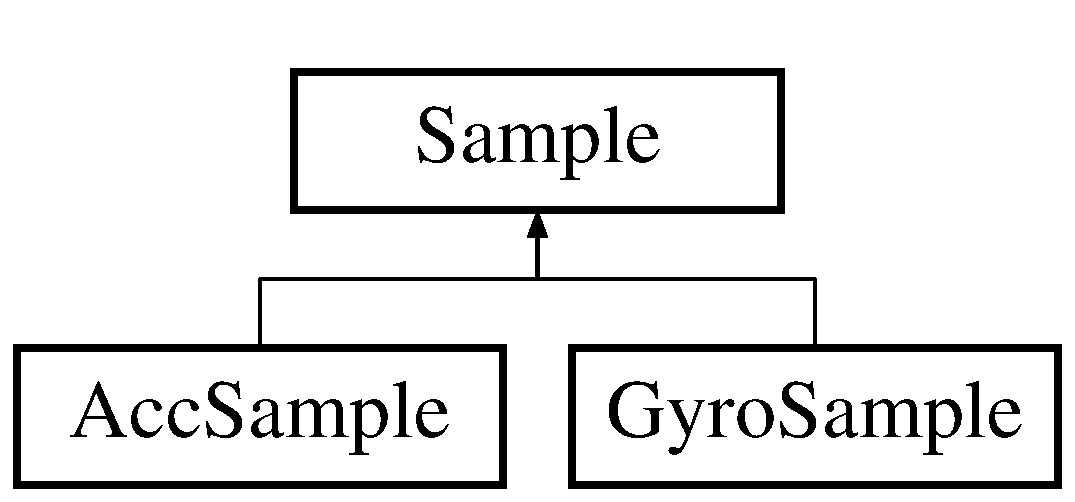
\includegraphics[height=2.000000cm]{class_sample}
\end{center}
\end{figure}
\subsection*{\-Public \-Member \-Functions}
\begin{DoxyCompactItemize}
\item 
\hypertarget{class_sample_a4f65c4a8bb86396782450121c7dc5ba5}{virtual void {\bfseries save} (ofstream \&out)=0}\label{class_sample_a4f65c4a8bb86396782450121c7dc5ba5}

\item 
\hypertarget{class_sample_ae728243bef5e290d46a2851ea2ce5fe2}{void {\bfseries set\-Log\-Type} (int l)}\label{class_sample_ae728243bef5e290d46a2851ea2ce5fe2}

\item 
\hypertarget{class_sample_aafff0e8223f3eafa001611a63f194c8a}{int {\bfseries get\-Log\-Type} () const }\label{class_sample_aafff0e8223f3eafa001611a63f194c8a}

\item 
\hypertarget{class_sample_a05edd06782fa94517b8daeb29e12057d}{void {\bfseries set\-Timestamp\-From\-Gesture\-Start} (unsigned long t)}\label{class_sample_a05edd06782fa94517b8daeb29e12057d}

\item 
\hypertarget{class_sample_a94a34fe92c0f8a89485042aaea458d94}{unsigned long {\bfseries get\-Timestamp\-From\-Gesture\-Start} () const }\label{class_sample_a94a34fe92c0f8a89485042aaea458d94}

\end{DoxyCompactItemize}
\subsection*{\-Protected \-Attributes}
\begin{DoxyCompactItemize}
\item 
\hypertarget{class_sample_a24ea733ab0a815949a57aca2a4740e33}{unsigned long {\bfseries rel\-Timestamp}}\label{class_sample_a24ea733ab0a815949a57aca2a4740e33}

\item 
\hypertarget{class_sample_a3a6454628c790459f41de5c83bf3ec7c}{int {\bfseries log\-Type}}\label{class_sample_a3a6454628c790459f41de5c83bf3ec7c}

\end{DoxyCompactItemize}


\subsection{\-Detailed \-Description}


\-Definition at line 15 of file sample.\-h.



\-The documentation for this class was generated from the following file\-:\begin{DoxyCompactItemize}
\item 
sample.\-h\end{DoxyCompactItemize}

\hypertarget{class_screen}{\section{Screen Class Reference}
\label{class_screen}\index{Screen@{Screen}}
}
\subsection*{Public Member Functions}
\begin{DoxyCompactItemize}
\item 
\hypertarget{class_screen_ad664ad8b3ba858a4b9a3798cd2a0e295}{{\bfseries Screen} (int x, int y)}\label{class_screen_ad664ad8b3ba858a4b9a3798cd2a0e295}

\item 
\hypertarget{class_screen_a7b45282430392ffa8b5891936363f8f8}{{\bfseries Screen} (const \hyperlink{struct_angel_1_1vec2}{vec2} \&new\-Size)}\label{class_screen_a7b45282430392ffa8b5891936363f8f8}

\item 
\hypertarget{class_screen_a478c5176fd4fdc8af48f2bd7e824329d}{void {\bfseries Size} (int x, int y)}\label{class_screen_a478c5176fd4fdc8af48f2bd7e824329d}

\item 
\hypertarget{class_screen_a5fa4071af08df619e7cb4311bc0efb45}{void {\bfseries Size} (const \hyperlink{struct_angel_1_1vec2}{vec2} \&new\-Size)}\label{class_screen_a5fa4071af08df619e7cb4311bc0efb45}

\item 
\hypertarget{class_screen_a6f22423a037d9cf406d3ca4dd79b94b5}{const \hyperlink{struct_angel_1_1vec2}{vec2} \& {\bfseries Size} (void)}\label{class_screen_a6f22423a037d9cf406d3ca4dd79b94b5}

\item 
\hypertarget{class_screen_aa9a4a2e113af54d7164463bef8e78471}{int {\bfseries Width} (void)}\label{class_screen_aa9a4a2e113af54d7164463bef8e78471}

\item 
\hypertarget{class_screen_ad532ef57bbdb9a1e1540812a02eece23}{int {\bfseries Height} (void)}\label{class_screen_ad532ef57bbdb9a1e1540812a02eece23}

\item 
\hypertarget{class_screen_a00be376c569ac4b71d770f34e297f332}{const \hyperlink{struct_angel_1_1vec2}{vec2} \& {\bfseries Center} (void)}\label{class_screen_a00be376c569ac4b71d770f34e297f332}

\item 
\hypertarget{class_screen_a434f489a1b9d40319f7f6dbbf11db456}{int {\bfseries Midpoint\-X} (void)}\label{class_screen_a434f489a1b9d40319f7f6dbbf11db456}

\item 
\hypertarget{class_screen_a7b574e8ded50718dc1523180102e2f41}{int {\bfseries Midpoint\-Y} (void)}\label{class_screen_a7b574e8ded50718dc1523180102e2f41}

\end{DoxyCompactItemize}
\subsection*{Public Attributes}
\begin{DoxyCompactItemize}
\item 
\hypertarget{class_screen_ae18e2382eee3c792f94d251ee58b3264}{\hyperlink{class_cameras}{Cameras} {\bfseries cam\-List}}\label{class_screen_ae18e2382eee3c792f94d251ee58b3264}

\end{DoxyCompactItemize}
\subsection*{Private Attributes}
\begin{DoxyCompactItemize}
\item 
\hypertarget{class_screen_a518fc6d0287e8d3cf44a1eb73f3be6e7}{\hyperlink{struct_angel_1_1vec2}{vec2} {\bfseries size}}\label{class_screen_a518fc6d0287e8d3cf44a1eb73f3be6e7}

\item 
\hypertarget{class_screen_a9aaa9c66b706c2186fa024bf139078f3}{\hyperlink{struct_angel_1_1vec2}{vec2} {\bfseries center}}\label{class_screen_a9aaa9c66b706c2186fa024bf139078f3}

\end{DoxyCompactItemize}


\subsection{Detailed Description}


Definition at line 8 of file Screen.\-hpp.



The documentation for this class was generated from the following files\-:\begin{DoxyCompactItemize}
\item 
Screen.\-hpp\item 
Screen.\-cpp\end{DoxyCompactItemize}

\hypertarget{class_training}{\section{Training Class Reference}
\label{class_training}\index{Training@{Training}}
}


Class \hyperlink{class_training}{Training} to save the individual training of a gesture.  




{\ttfamily \#include $<$training.\-h$>$}

\subsection*{Public Member Functions}
\begin{DoxyCompactItemize}
\item 
\hypertarget{class_training_af98b1bc7ed710e2fa008a72ad29dbdae}{\hyperlink{class_training_af98b1bc7ed710e2fa008a72ad29dbdae}{Training} ()}\label{class_training_af98b1bc7ed710e2fa008a72ad29dbdae}

\begin{DoxyCompactList}\small\item\em Default constructor. \end{DoxyCompactList}\item 
\hypertarget{class_training_a6db6a1a9302641ca0d74308e583667af}{\hyperlink{class_training_a6db6a1a9302641ca0d74308e583667af}{$\sim$\-Training} ()}\label{class_training_a6db6a1a9302641ca0d74308e583667af}

\begin{DoxyCompactList}\small\item\em \hyperlink{class_dataset}{Dataset} destructor, which calls clear. \end{DoxyCompactList}\item 
bool \hyperlink{class_training_a9399c15218729fefd018b7cd3d303319}{load\-Training} (ifstream \&)
\begin{DoxyCompactList}\small\item\em Load a training stored in a file. \end{DoxyCompactList}\item 
void \hyperlink{class_training_a53db95eff724d953faaca919708bc10f}{save} (ofstream \&) const 
\begin{DoxyCompactList}\small\item\em Save the training into a file for training and recognition. \end{DoxyCompactList}\item 
void \hyperlink{class_training_a3b7366795dfe6861f8db51b8dc4a719e}{add\-Sample} (\hyperlink{class_sample}{Sample} $\ast$)
\begin{DoxyCompactList}\small\item\em Add a new training to the dataset. \end{DoxyCompactList}\item 
void \hyperlink{class_training_aa8b430a49b5aaa8410c9288e19f4bbcb}{clear} ()
\begin{DoxyCompactList}\small\item\em Delete all samples and clear the buffer. \end{DoxyCompactList}\item 
const \hyperlink{class_sample}{Sample} $\ast$ \hyperlink{class_training_a24c833bf0a60fc96cc09bc86b4de04ba}{sample\-At} (unsigned int i) const 
\begin{DoxyCompactList}\small\item\em Returns the i-\/th sample of the training as a constant pointer. \end{DoxyCompactList}\item 
\hyperlink{class_sample}{Sample} $\ast$ \hyperlink{class_training_ada77c7d75f23c04619f33dce4a46115d}{sample\-At} (unsigned int i)
\begin{DoxyCompactList}\small\item\em Returns the i-\/th sample of the training as a pointer. \end{DoxyCompactList}\item 
\hypertarget{class_training_a34cd1e59fb499746963c510de4ea8a31}{unsigned int \hyperlink{class_training_a34cd1e59fb499746963c510de4ea8a31}{size} () const }\label{class_training_a34cd1e59fb499746963c510de4ea8a31}

\begin{DoxyCompactList}\small\item\em Number of samples in the current training. \end{DoxyCompactList}\item 
\hypertarget{class_training_a94d0694609b43099eade91b194212e85}{void {\bfseries set\-Timestamp\-From\-Midnight} (unsigned long ts)}\label{class_training_a94d0694609b43099eade91b194212e85}

\item 
\hypertarget{class_training_af98b1bc7ed710e2fa008a72ad29dbdae}{\hyperlink{class_training_af98b1bc7ed710e2fa008a72ad29dbdae}{Training} ()}\label{class_training_af98b1bc7ed710e2fa008a72ad29dbdae}

\begin{DoxyCompactList}\small\item\em Constructor void. \end{DoxyCompactList}\item 
\hypertarget{class_training_aaa3229d32dbbddf33db5c66dae89a02d}{{\bfseries Training} (Log\-Type l)}\label{class_training_aaa3229d32dbbddf33db5c66dae89a02d}

\item 
\hypertarget{class_training_a9399c15218729fefd018b7cd3d303319}{void {\bfseries load\-Training} (ifstream \&)}\label{class_training_a9399c15218729fefd018b7cd3d303319}

\item 
\hypertarget{class_training_a53db95eff724d953faaca919708bc10f}{void {\bfseries save} (ofstream \&) const }\label{class_training_a53db95eff724d953faaca919708bc10f}

\item 
\hypertarget{class_training_a3b7366795dfe6861f8db51b8dc4a719e}{void {\bfseries add\-Sample} (\hyperlink{class_sample}{Sample} $\ast$)}\label{class_training_a3b7366795dfe6861f8db51b8dc4a719e}

\item 
\hypertarget{class_training_aa8b430a49b5aaa8410c9288e19f4bbcb}{void {\bfseries clear} ()}\label{class_training_aa8b430a49b5aaa8410c9288e19f4bbcb}

\item 
\hypertarget{class_training_a24c833bf0a60fc96cc09bc86b4de04ba}{const \hyperlink{class_sample}{Sample} $\ast$ {\bfseries sample\-At} (unsigned int i) const }\label{class_training_a24c833bf0a60fc96cc09bc86b4de04ba}

\item 
\hypertarget{class_training_ada77c7d75f23c04619f33dce4a46115d}{\hyperlink{class_sample}{Sample} $\ast$ {\bfseries sample\-At} (unsigned int i)}\label{class_training_ada77c7d75f23c04619f33dce4a46115d}

\item 
\hypertarget{class_training_a70170c11ac3fe14b840fdb5484ad4247}{void {\bfseries set\-Log\-Type} (Log\-Type l)}\label{class_training_a70170c11ac3fe14b840fdb5484ad4247}

\item 
\hypertarget{class_training_af43ee4618a0620d940d95d88470440d4}{Log\-Type {\bfseries get\-Log\-Type} () const }\label{class_training_af43ee4618a0620d940d95d88470440d4}

\item 
\hypertarget{class_training_a34cd1e59fb499746963c510de4ea8a31}{unsigned int {\bfseries size} () const }\label{class_training_a34cd1e59fb499746963c510de4ea8a31}

\end{DoxyCompactItemize}
\subsection*{Protected Member Functions}
\begin{DoxyCompactItemize}
\item 
\hypertarget{class_training_adab700ca2a1d928fcceb0a7d1c515830}{void {\bfseries load\-Acc\-Training} (ifstream \&infile)}\label{class_training_adab700ca2a1d928fcceb0a7d1c515830}

\end{DoxyCompactItemize}
\subsection*{Private Attributes}
\begin{DoxyCompactItemize}
\item 
\hypertarget{class_training_a552318082a3618fd28e38cd4f37d8bf8}{vector$<$ \hyperlink{class_sample}{Sample} $\ast$ $>$ {\bfseries samples}}\label{class_training_a552318082a3618fd28e38cd4f37d8bf8}

\item 
\hypertarget{class_training_a9eac3dfdc171b6c301f1d2a9b3dfd846}{unsigned long {\bfseries timestamp}}\label{class_training_a9eac3dfdc171b6c301f1d2a9b3dfd846}

\item 
\hypertarget{class_training_a252abea8bd5504538e2d7f2a415d4927}{Log\-Type {\bfseries log\-Type}}\label{class_training_a252abea8bd5504538e2d7f2a415d4927}

\end{DoxyCompactItemize}


\subsection{Detailed Description}
Class \hyperlink{class_training}{Training} to save the individual training of a gesture. 

Definition at line 17 of file wiic\-\_\-r90/src/log/training.\-h.



\subsection{Member Function Documentation}
\hypertarget{class_training_a3b7366795dfe6861f8db51b8dc4a719e}{\index{Training@{Training}!add\-Sample@{add\-Sample}}
\index{add\-Sample@{add\-Sample}!Training@{Training}}
\subsubsection[{add\-Sample}]{\setlength{\rightskip}{0pt plus 5cm}void Training\-::add\-Sample (
\begin{DoxyParamCaption}
\item[{{\bf Sample} $\ast$}]{sample}
\end{DoxyParamCaption}
)}}\label{class_training_a3b7366795dfe6861f8db51b8dc4a719e}


Add a new training to the dataset. 


\begin{DoxyParams}{Parameters}
{\em sample} & Add a sample to the training set. \\
\hline
\end{DoxyParams}


Definition at line 67 of file wiic\-\_\-r90/src/log/training.\-cpp.

\hypertarget{class_training_aa8b430a49b5aaa8410c9288e19f4bbcb}{\index{Training@{Training}!clear@{clear}}
\index{clear@{clear}!Training@{Training}}
\subsubsection[{clear}]{\setlength{\rightskip}{0pt plus 5cm}void Training\-::clear (
\begin{DoxyParamCaption}
{}
\end{DoxyParamCaption}
)}}\label{class_training_aa8b430a49b5aaa8410c9288e19f4bbcb}


Delete all samples and clear the buffer. 

This method will take care of freeing the memory of each sample in the training set, hence you don't need to free them in your code. 

Definition at line 88 of file wiic\-\_\-r90/src/log/training.\-cpp.

\hypertarget{class_training_a9399c15218729fefd018b7cd3d303319}{\index{Training@{Training}!load\-Training@{load\-Training}}
\index{load\-Training@{load\-Training}!Training@{Training}}
\subsubsection[{load\-Training}]{\setlength{\rightskip}{0pt plus 5cm}void Training\-::load\-Training (
\begin{DoxyParamCaption}
\item[{ifstream \&}]{training}
\end{DoxyParamCaption}
)}}\label{class_training_a9399c15218729fefd018b7cd3d303319}


Load a training stored in a file. 


\begin{DoxyParams}{Parameters}
{\em training} & File stream of the contained training \\
\hline
\end{DoxyParams}


Definition at line 16 of file wiic\-\_\-r90/src/log/training.\-cpp.

\hypertarget{class_training_a24c833bf0a60fc96cc09bc86b4de04ba}{\index{Training@{Training}!sample\-At@{sample\-At}}
\index{sample\-At@{sample\-At}!Training@{Training}}
\subsubsection[{sample\-At}]{\setlength{\rightskip}{0pt plus 5cm}const {\bf Sample}$\ast$ Training\-::sample\-At (
\begin{DoxyParamCaption}
\item[{unsigned int}]{i}
\end{DoxyParamCaption}
) const\hspace{0.3cm}{\ttfamily [inline]}}}\label{class_training_a24c833bf0a60fc96cc09bc86b4de04ba}


Returns the i-\/th sample of the training as a constant pointer. 


\begin{DoxyParams}{Parameters}
{\em i} & \hyperlink{class_sample}{Sample} index in the training set \\
\hline
\end{DoxyParams}


Definition at line 36 of file wiic\-\_\-r90/src/log/training.\-h.

\hypertarget{class_training_ada77c7d75f23c04619f33dce4a46115d}{\index{Training@{Training}!sample\-At@{sample\-At}}
\index{sample\-At@{sample\-At}!Training@{Training}}
\subsubsection[{sample\-At}]{\setlength{\rightskip}{0pt plus 5cm}{\bf Sample}$\ast$ Training\-::sample\-At (
\begin{DoxyParamCaption}
\item[{unsigned int}]{i}
\end{DoxyParamCaption}
)\hspace{0.3cm}{\ttfamily [inline]}}}\label{class_training_ada77c7d75f23c04619f33dce4a46115d}


Returns the i-\/th sample of the training as a pointer. 


\begin{DoxyParams}{Parameters}
{\em i} & \hyperlink{class_sample}{Sample} index in the training set \\
\hline
\end{DoxyParams}


Definition at line 50 of file wiic\-\_\-r90/src/log/training.\-h.

\hypertarget{class_training_a53db95eff724d953faaca919708bc10f}{\index{Training@{Training}!save@{save}}
\index{save@{save}!Training@{Training}}
\subsubsection[{save}]{\setlength{\rightskip}{0pt plus 5cm}void Training\-::save (
\begin{DoxyParamCaption}
\item[{ofstream \&}]{out}
\end{DoxyParamCaption}
) const}}\label{class_training_a53db95eff724d953faaca919708bc10f}


Save the training into a file for training and recognition. 


\begin{DoxyParams}{Parameters}
{\em out} & Stream of the destination file \\
\hline
\end{DoxyParams}


Definition at line 50 of file wiic\-\_\-r90/src/log/training.\-cpp.



The documentation for this class was generated from the following files\-:\begin{DoxyCompactItemize}
\item 
wiic\-\_\-r90/src/log/training.\-h\item 
wiic\-\_\-v1.\-1/src/log/training.\-h\item 
wiic\-\_\-r90/src/log/training.\-cpp\item 
wiic\-\_\-v1.\-1/src/log/training.\-cpp\end{DoxyCompactItemize}

\hypertarget{struct_angel_1_1vec2}{\section{\-Angel\-:\-:vec2 \-Struct \-Reference}
\label{struct_angel_1_1vec2}\index{\-Angel\-::vec2@{\-Angel\-::vec2}}
}
\subsection*{\-Public \-Member \-Functions}
\begin{DoxyCompactItemize}
\item 
\hypertarget{struct_angel_1_1vec2_ab2463ddb6aaaa67251004b90f03530fa}{{\bfseries vec2} (\-G\-Lfloat s=\-G\-Lfloat(0.\-0))}\label{struct_angel_1_1vec2_ab2463ddb6aaaa67251004b90f03530fa}

\item 
\hypertarget{struct_angel_1_1vec2_a8e55cc0bb681ca7a747721cab122d830}{{\bfseries vec2} (\-G\-Lfloat x, \-G\-Lfloat y)}\label{struct_angel_1_1vec2_a8e55cc0bb681ca7a747721cab122d830}

\item 
\hypertarget{struct_angel_1_1vec2_aa2ec5b81c4b97019486b0595db6f35a1}{{\bfseries vec2} (const \hyperlink{struct_angel_1_1vec2}{vec2} \&v)}\label{struct_angel_1_1vec2_aa2ec5b81c4b97019486b0595db6f35a1}

\item 
\hypertarget{struct_angel_1_1vec2_a2605b81b6230d8d9184f3a06ff3fe7ae}{\-G\-Lfloat \& {\bfseries operator\mbox{[}$\,$\mbox{]}} (int i)}\label{struct_angel_1_1vec2_a2605b81b6230d8d9184f3a06ff3fe7ae}

\item 
\hypertarget{struct_angel_1_1vec2_a83725a082bca8ea73a2171bb4596c1bd}{const \-G\-Lfloat {\bfseries operator\mbox{[}$\,$\mbox{]}} (int i) const }\label{struct_angel_1_1vec2_a83725a082bca8ea73a2171bb4596c1bd}

\item 
\hypertarget{struct_angel_1_1vec2_a3b29693925c8026f75572dd13cefee5a}{\hyperlink{struct_angel_1_1vec2}{vec2} {\bfseries operator-\/} () const }\label{struct_angel_1_1vec2_a3b29693925c8026f75572dd13cefee5a}

\item 
\hypertarget{struct_angel_1_1vec2_a93606208e7b65d4bb8004f498b22934f}{\hyperlink{struct_angel_1_1vec2}{vec2} {\bfseries operator+} (const \hyperlink{struct_angel_1_1vec2}{vec2} \&v) const }\label{struct_angel_1_1vec2_a93606208e7b65d4bb8004f498b22934f}

\item 
\hypertarget{struct_angel_1_1vec2_a2d3d52e1b4693fdb860c2ef246e0d4d8}{\hyperlink{struct_angel_1_1vec2}{vec2} {\bfseries operator-\/} (const \hyperlink{struct_angel_1_1vec2}{vec2} \&v) const }\label{struct_angel_1_1vec2_a2d3d52e1b4693fdb860c2ef246e0d4d8}

\item 
\hypertarget{struct_angel_1_1vec2_ac5615b2494e3f8824f9fa127ba122b67}{\hyperlink{struct_angel_1_1vec2}{vec2} {\bfseries operator$\ast$} (const \-G\-Lfloat s) const }\label{struct_angel_1_1vec2_ac5615b2494e3f8824f9fa127ba122b67}

\item 
\hypertarget{struct_angel_1_1vec2_a3b4a9670b53342b870e3a14c8164c613}{\hyperlink{struct_angel_1_1vec2}{vec2} {\bfseries operator$\ast$} (const \hyperlink{struct_angel_1_1vec2}{vec2} \&v) const }\label{struct_angel_1_1vec2_a3b4a9670b53342b870e3a14c8164c613}

\item 
\hypertarget{struct_angel_1_1vec2_a522a6aaa64c361b86f6c2469cbd8ca92}{\hyperlink{struct_angel_1_1vec2}{vec2} {\bfseries operator/} (const \-G\-Lfloat s) const }\label{struct_angel_1_1vec2_a522a6aaa64c361b86f6c2469cbd8ca92}

\item 
\hypertarget{struct_angel_1_1vec2_a0d7255e85aa7765f6e54160c2f6d6d40}{\hyperlink{struct_angel_1_1vec2}{vec2} \& {\bfseries operator+=} (const \hyperlink{struct_angel_1_1vec2}{vec2} \&v)}\label{struct_angel_1_1vec2_a0d7255e85aa7765f6e54160c2f6d6d40}

\item 
\hypertarget{struct_angel_1_1vec2_ad650808486497a53572561c664c6e865}{\hyperlink{struct_angel_1_1vec2}{vec2} \& {\bfseries operator-\/=} (const \hyperlink{struct_angel_1_1vec2}{vec2} \&v)}\label{struct_angel_1_1vec2_ad650808486497a53572561c664c6e865}

\item 
\hypertarget{struct_angel_1_1vec2_afb79fcf6de3814fd875d1402e160097a}{\hyperlink{struct_angel_1_1vec2}{vec2} \& {\bfseries operator$\ast$=} (const \-G\-Lfloat s)}\label{struct_angel_1_1vec2_afb79fcf6de3814fd875d1402e160097a}

\item 
\hypertarget{struct_angel_1_1vec2_aa13326415630734f076da6e7466ea195}{\hyperlink{struct_angel_1_1vec2}{vec2} \& {\bfseries operator$\ast$=} (const \hyperlink{struct_angel_1_1vec2}{vec2} \&v)}\label{struct_angel_1_1vec2_aa13326415630734f076da6e7466ea195}

\item 
\hypertarget{struct_angel_1_1vec2_a0739a7464b89dc5b40fae5c423711e11}{\hyperlink{struct_angel_1_1vec2}{vec2} \& {\bfseries operator/=} (const \-G\-Lfloat s)}\label{struct_angel_1_1vec2_a0739a7464b89dc5b40fae5c423711e11}

\item 
\hypertarget{struct_angel_1_1vec2_a5c3d2082bcc18734fde3689dbc605104}{{\bfseries operator const G\-Lfloat $\ast$} () const }\label{struct_angel_1_1vec2_a5c3d2082bcc18734fde3689dbc605104}

\item 
\hypertarget{struct_angel_1_1vec2_a8989f46bc38bb87bc2f6ea81f66c8545}{{\bfseries operator G\-Lfloat $\ast$} ()}\label{struct_angel_1_1vec2_a8989f46bc38bb87bc2f6ea81f66c8545}

\item 
\hypertarget{struct_angel_1_1vec2_ab2463ddb6aaaa67251004b90f03530fa}{{\bfseries vec2} (\-G\-Lfloat s=\-G\-Lfloat(0.\-0))}\label{struct_angel_1_1vec2_ab2463ddb6aaaa67251004b90f03530fa}

\item 
\hypertarget{struct_angel_1_1vec2_a8e55cc0bb681ca7a747721cab122d830}{{\bfseries vec2} (\-G\-Lfloat x, \-G\-Lfloat y)}\label{struct_angel_1_1vec2_a8e55cc0bb681ca7a747721cab122d830}

\item 
\hypertarget{struct_angel_1_1vec2_aa2ec5b81c4b97019486b0595db6f35a1}{{\bfseries vec2} (const \hyperlink{struct_angel_1_1vec2}{vec2} \&v)}\label{struct_angel_1_1vec2_aa2ec5b81c4b97019486b0595db6f35a1}

\item 
\hypertarget{struct_angel_1_1vec2_a2605b81b6230d8d9184f3a06ff3fe7ae}{\-G\-Lfloat \& {\bfseries operator\mbox{[}$\,$\mbox{]}} (int i)}\label{struct_angel_1_1vec2_a2605b81b6230d8d9184f3a06ff3fe7ae}

\item 
\hypertarget{struct_angel_1_1vec2_a83725a082bca8ea73a2171bb4596c1bd}{const \-G\-Lfloat {\bfseries operator\mbox{[}$\,$\mbox{]}} (int i) const }\label{struct_angel_1_1vec2_a83725a082bca8ea73a2171bb4596c1bd}

\item 
\hypertarget{struct_angel_1_1vec2_a3b29693925c8026f75572dd13cefee5a}{\hyperlink{struct_angel_1_1vec2}{vec2} {\bfseries operator-\/} () const }\label{struct_angel_1_1vec2_a3b29693925c8026f75572dd13cefee5a}

\item 
\hypertarget{struct_angel_1_1vec2_a93606208e7b65d4bb8004f498b22934f}{\hyperlink{struct_angel_1_1vec2}{vec2} {\bfseries operator+} (const \hyperlink{struct_angel_1_1vec2}{vec2} \&v) const }\label{struct_angel_1_1vec2_a93606208e7b65d4bb8004f498b22934f}

\item 
\hypertarget{struct_angel_1_1vec2_a2d3d52e1b4693fdb860c2ef246e0d4d8}{\hyperlink{struct_angel_1_1vec2}{vec2} {\bfseries operator-\/} (const \hyperlink{struct_angel_1_1vec2}{vec2} \&v) const }\label{struct_angel_1_1vec2_a2d3d52e1b4693fdb860c2ef246e0d4d8}

\item 
\hypertarget{struct_angel_1_1vec2_ac5615b2494e3f8824f9fa127ba122b67}{\hyperlink{struct_angel_1_1vec2}{vec2} {\bfseries operator$\ast$} (const \-G\-Lfloat s) const }\label{struct_angel_1_1vec2_ac5615b2494e3f8824f9fa127ba122b67}

\item 
\hypertarget{struct_angel_1_1vec2_a3b4a9670b53342b870e3a14c8164c613}{\hyperlink{struct_angel_1_1vec2}{vec2} {\bfseries operator$\ast$} (const \hyperlink{struct_angel_1_1vec2}{vec2} \&v) const }\label{struct_angel_1_1vec2_a3b4a9670b53342b870e3a14c8164c613}

\item 
\hypertarget{struct_angel_1_1vec2_a522a6aaa64c361b86f6c2469cbd8ca92}{\hyperlink{struct_angel_1_1vec2}{vec2} {\bfseries operator/} (const \-G\-Lfloat s) const }\label{struct_angel_1_1vec2_a522a6aaa64c361b86f6c2469cbd8ca92}

\item 
\hypertarget{struct_angel_1_1vec2_a0d7255e85aa7765f6e54160c2f6d6d40}{\hyperlink{struct_angel_1_1vec2}{vec2} \& {\bfseries operator+=} (const \hyperlink{struct_angel_1_1vec2}{vec2} \&v)}\label{struct_angel_1_1vec2_a0d7255e85aa7765f6e54160c2f6d6d40}

\item 
\hypertarget{struct_angel_1_1vec2_ad650808486497a53572561c664c6e865}{\hyperlink{struct_angel_1_1vec2}{vec2} \& {\bfseries operator-\/=} (const \hyperlink{struct_angel_1_1vec2}{vec2} \&v)}\label{struct_angel_1_1vec2_ad650808486497a53572561c664c6e865}

\item 
\hypertarget{struct_angel_1_1vec2_afb79fcf6de3814fd875d1402e160097a}{\hyperlink{struct_angel_1_1vec2}{vec2} \& {\bfseries operator$\ast$=} (const \-G\-Lfloat s)}\label{struct_angel_1_1vec2_afb79fcf6de3814fd875d1402e160097a}

\item 
\hypertarget{struct_angel_1_1vec2_aa13326415630734f076da6e7466ea195}{\hyperlink{struct_angel_1_1vec2}{vec2} \& {\bfseries operator$\ast$=} (const \hyperlink{struct_angel_1_1vec2}{vec2} \&v)}\label{struct_angel_1_1vec2_aa13326415630734f076da6e7466ea195}

\item 
\hypertarget{struct_angel_1_1vec2_a0739a7464b89dc5b40fae5c423711e11}{\hyperlink{struct_angel_1_1vec2}{vec2} \& {\bfseries operator/=} (const \-G\-Lfloat s)}\label{struct_angel_1_1vec2_a0739a7464b89dc5b40fae5c423711e11}

\item 
\hypertarget{struct_angel_1_1vec2_a5c3d2082bcc18734fde3689dbc605104}{{\bfseries operator const G\-Lfloat $\ast$} () const }\label{struct_angel_1_1vec2_a5c3d2082bcc18734fde3689dbc605104}

\item 
\hypertarget{struct_angel_1_1vec2_a8989f46bc38bb87bc2f6ea81f66c8545}{{\bfseries operator G\-Lfloat $\ast$} ()}\label{struct_angel_1_1vec2_a8989f46bc38bb87bc2f6ea81f66c8545}

\end{DoxyCompactItemize}
\subsection*{\-Public \-Attributes}
\begin{DoxyCompactItemize}
\item 
\hypertarget{struct_angel_1_1vec2_ab99b91871c08bbf76bf4a5e554ccac8f}{\-G\-Lfloat {\bfseries x}}\label{struct_angel_1_1vec2_ab99b91871c08bbf76bf4a5e554ccac8f}

\item 
\hypertarget{struct_angel_1_1vec2_a9f0e4c33e7884eca47d771ccfd4ea0bd}{\-G\-Lfloat {\bfseries y}}\label{struct_angel_1_1vec2_a9f0e4c33e7884eca47d771ccfd4ea0bd}

\end{DoxyCompactItemize}
\subsection*{\-Friends}
\begin{DoxyCompactItemize}
\item 
\hypertarget{struct_angel_1_1vec2_a1f371c4b26f86deb4d296dfff8ff1fc1}{\hyperlink{struct_angel_1_1vec2}{vec2} {\bfseries operator$\ast$} (const \-G\-Lfloat s, const \hyperlink{struct_angel_1_1vec2}{vec2} \&v)}\label{struct_angel_1_1vec2_a1f371c4b26f86deb4d296dfff8ff1fc1}

\item 
\hypertarget{struct_angel_1_1vec2_a5533e582fe94db90861caa394494f2cf}{std\-::ostream \& {\bfseries operator$<$$<$} (std\-::ostream \&os, const \hyperlink{struct_angel_1_1vec2}{vec2} \&v)}\label{struct_angel_1_1vec2_a5533e582fe94db90861caa394494f2cf}

\item 
\hypertarget{struct_angel_1_1vec2_af8cf130207f2cf5866ac13049e956c75}{std\-::istream \& {\bfseries operator$>$$>$} (std\-::istream \&is, \hyperlink{struct_angel_1_1vec2}{vec2} \&v)}\label{struct_angel_1_1vec2_af8cf130207f2cf5866ac13049e956c75}

\item 
\hypertarget{struct_angel_1_1vec2_a1f371c4b26f86deb4d296dfff8ff1fc1}{\hyperlink{struct_angel_1_1vec2}{vec2} {\bfseries operator$\ast$} (const \-G\-Lfloat s, const \hyperlink{struct_angel_1_1vec2}{vec2} \&v)}\label{struct_angel_1_1vec2_a1f371c4b26f86deb4d296dfff8ff1fc1}

\item 
\hypertarget{struct_angel_1_1vec2_a5533e582fe94db90861caa394494f2cf}{std\-::ostream \& {\bfseries operator$<$$<$} (std\-::ostream \&os, const \hyperlink{struct_angel_1_1vec2}{vec2} \&v)}\label{struct_angel_1_1vec2_a5533e582fe94db90861caa394494f2cf}

\item 
\hypertarget{struct_angel_1_1vec2_af8cf130207f2cf5866ac13049e956c75}{std\-::istream \& {\bfseries operator$>$$>$} (std\-::istream \&is, \hyperlink{struct_angel_1_1vec2}{vec2} \&v)}\label{struct_angel_1_1vec2_af8cf130207f2cf5866ac13049e956c75}

\end{DoxyCompactItemize}


\subsection{\-Detailed \-Description}


\-Definition at line 19 of file vec.\-h.



\-The documentation for this struct was generated from the following files\-:\begin{DoxyCompactItemize}
\item 
vec.\-h\item 
vec.\-hpp\end{DoxyCompactItemize}

\hypertarget{structvec2b__t}{\section{vec2b\-\_\-t Struct Reference}
\label{structvec2b__t}\index{vec2b\-\_\-t@{vec2b\-\_\-t}}
}


Unsigned x,y byte vector.  




{\ttfamily \#include $<$wiic\-\_\-structs.\-h$>$}

\subsection*{Public Attributes}
\begin{DoxyCompactItemize}
\item 
\hypertarget{structvec2b__t_a770aacd26e2799bccfecd8eeb4f16092}{\hyperlink{wiic__macros_8h_a0c8186d9b9b7880309c27230bbb5e69d}{byte} {\bfseries x}}\label{structvec2b__t_a770aacd26e2799bccfecd8eeb4f16092}

\item 
\hypertarget{structvec2b__t_ad69850e7b8fd19a9cb69431d5dbfab83}{\hyperlink{wiic__macros_8h_a0c8186d9b9b7880309c27230bbb5e69d}{byte} {\bfseries y}}\label{structvec2b__t_ad69850e7b8fd19a9cb69431d5dbfab83}

\end{DoxyCompactItemize}


\subsection{Detailed Description}
Unsigned x,y byte vector. 

Definition at line 66 of file wiic\-\_\-structs.\-h.



The documentation for this struct was generated from the following file\-:\begin{DoxyCompactItemize}
\item 
\hyperlink{wiic__structs_8h}{wiic\-\_\-structs.\-h}\end{DoxyCompactItemize}

\hypertarget{struct_angel_1_1vec3}{\section{\-Angel\-:\-:vec3 \-Struct \-Reference}
\label{struct_angel_1_1vec3}\index{\-Angel\-::vec3@{\-Angel\-::vec3}}
}
\subsection*{\-Public \-Member \-Functions}
\begin{DoxyCompactItemize}
\item 
\hypertarget{struct_angel_1_1vec3_a420358f913d30a659761e3a86026cd59}{{\bfseries vec3} (\-G\-Lfloat s=\-G\-Lfloat(0.\-0))}\label{struct_angel_1_1vec3_a420358f913d30a659761e3a86026cd59}

\item 
\hypertarget{struct_angel_1_1vec3_a9970b9133cd349d038456ae7309fbeba}{{\bfseries vec3} (\-G\-Lfloat x, \-G\-Lfloat y, \-G\-Lfloat z)}\label{struct_angel_1_1vec3_a9970b9133cd349d038456ae7309fbeba}

\item 
\hypertarget{struct_angel_1_1vec3_a3af0b92e9cb01f0cda2f66c007e196c9}{{\bfseries vec3} (const \hyperlink{struct_angel_1_1vec3}{vec3} \&v)}\label{struct_angel_1_1vec3_a3af0b92e9cb01f0cda2f66c007e196c9}

\item 
\hypertarget{struct_angel_1_1vec3_a597ff15b14f6bd9e75382525f6da00bd}{{\bfseries vec3} (const \hyperlink{struct_angel_1_1vec2}{vec2} \&v, const float f)}\label{struct_angel_1_1vec3_a597ff15b14f6bd9e75382525f6da00bd}

\item 
\hypertarget{struct_angel_1_1vec3_a571e36d7c9542eb3464b8fde016d040d}{\-G\-Lfloat \& {\bfseries operator\mbox{[}$\,$\mbox{]}} (int i)}\label{struct_angel_1_1vec3_a571e36d7c9542eb3464b8fde016d040d}

\item 
\hypertarget{struct_angel_1_1vec3_ad78e907775d490a69aa879a34e7dfe5c}{const \-G\-Lfloat {\bfseries operator\mbox{[}$\,$\mbox{]}} (int i) const }\label{struct_angel_1_1vec3_ad78e907775d490a69aa879a34e7dfe5c}

\item 
\hypertarget{struct_angel_1_1vec3_a5ec954ef19e3d1ceed6ce25ebe32c3ee}{\hyperlink{struct_angel_1_1vec3}{vec3} {\bfseries operator-\/} () const }\label{struct_angel_1_1vec3_a5ec954ef19e3d1ceed6ce25ebe32c3ee}

\item 
\hypertarget{struct_angel_1_1vec3_a320586bc86a5abd0ac991a3e51485ef6}{\hyperlink{struct_angel_1_1vec3}{vec3} {\bfseries operator+} (const \hyperlink{struct_angel_1_1vec3}{vec3} \&v) const }\label{struct_angel_1_1vec3_a320586bc86a5abd0ac991a3e51485ef6}

\item 
\hypertarget{struct_angel_1_1vec3_a947a9982285c993f79d8ab3afc4da2c8}{\hyperlink{struct_angel_1_1vec3}{vec3} {\bfseries operator-\/} (const \hyperlink{struct_angel_1_1vec3}{vec3} \&v) const }\label{struct_angel_1_1vec3_a947a9982285c993f79d8ab3afc4da2c8}

\item 
\hypertarget{struct_angel_1_1vec3_aa2d45d74dee02720c82757f03263e8ae}{\hyperlink{struct_angel_1_1vec3}{vec3} {\bfseries operator$\ast$} (const \-G\-Lfloat s) const }\label{struct_angel_1_1vec3_aa2d45d74dee02720c82757f03263e8ae}

\item 
\hypertarget{struct_angel_1_1vec3_aa6709e55b49d756a9b00e038adc68438}{\hyperlink{struct_angel_1_1vec3}{vec3} {\bfseries operator$\ast$} (const \hyperlink{struct_angel_1_1vec3}{vec3} \&v) const }\label{struct_angel_1_1vec3_aa6709e55b49d756a9b00e038adc68438}

\item 
\hypertarget{struct_angel_1_1vec3_ab072ed9282da0217c26b8dae2c6bf978}{\hyperlink{struct_angel_1_1vec3}{vec3} {\bfseries operator/} (const \-G\-Lfloat s) const }\label{struct_angel_1_1vec3_ab072ed9282da0217c26b8dae2c6bf978}

\item 
\hypertarget{struct_angel_1_1vec3_abe9f854bc044ab4461882c635b197102}{\hyperlink{struct_angel_1_1vec3}{vec3} \& {\bfseries operator+=} (const \hyperlink{struct_angel_1_1vec3}{vec3} \&v)}\label{struct_angel_1_1vec3_abe9f854bc044ab4461882c635b197102}

\item 
\hypertarget{struct_angel_1_1vec3_ada518593451bbc8b9529ddd36284402f}{\hyperlink{struct_angel_1_1vec3}{vec3} \& {\bfseries operator-\/=} (const \hyperlink{struct_angel_1_1vec3}{vec3} \&v)}\label{struct_angel_1_1vec3_ada518593451bbc8b9529ddd36284402f}

\item 
\hypertarget{struct_angel_1_1vec3_ab825bec2ce97dc35aa4835758ec51270}{\hyperlink{struct_angel_1_1vec3}{vec3} \& {\bfseries operator$\ast$=} (const \-G\-Lfloat s)}\label{struct_angel_1_1vec3_ab825bec2ce97dc35aa4835758ec51270}

\item 
\hypertarget{struct_angel_1_1vec3_a54e75f1d64f773d99f0d5e80b031142b}{\hyperlink{struct_angel_1_1vec3}{vec3} \& {\bfseries operator$\ast$=} (const \hyperlink{struct_angel_1_1vec3}{vec3} \&v)}\label{struct_angel_1_1vec3_a54e75f1d64f773d99f0d5e80b031142b}

\item 
\hypertarget{struct_angel_1_1vec3_ae3ac03ba1ce7c8bbb8dfe07c7e0d06d9}{\hyperlink{struct_angel_1_1vec3}{vec3} \& {\bfseries operator/=} (const \-G\-Lfloat s)}\label{struct_angel_1_1vec3_ae3ac03ba1ce7c8bbb8dfe07c7e0d06d9}

\item 
\hypertarget{struct_angel_1_1vec3_a81f4a99d68722e756664907dcb07fb92}{{\bfseries operator const G\-Lfloat $\ast$} () const }\label{struct_angel_1_1vec3_a81f4a99d68722e756664907dcb07fb92}

\item 
\hypertarget{struct_angel_1_1vec3_ab92761f9bc4454117c1dd39a7d87c1b0}{{\bfseries operator G\-Lfloat $\ast$} ()}\label{struct_angel_1_1vec3_ab92761f9bc4454117c1dd39a7d87c1b0}

\end{DoxyCompactItemize}
\subsection*{\-Public \-Attributes}
\begin{DoxyCompactItemize}
\item 
\hypertarget{struct_angel_1_1vec3_a758dbe298cc37615770c30a73066253d}{\-G\-Lfloat {\bfseries x}}\label{struct_angel_1_1vec3_a758dbe298cc37615770c30a73066253d}

\item 
\hypertarget{struct_angel_1_1vec3_a02608203e694798c3118d5b55a0e0048}{\-G\-Lfloat {\bfseries y}}\label{struct_angel_1_1vec3_a02608203e694798c3118d5b55a0e0048}

\item 
\hypertarget{struct_angel_1_1vec3_afa2e7231c4170ddedb556ef5f7941cbc}{\-G\-Lfloat {\bfseries z}}\label{struct_angel_1_1vec3_afa2e7231c4170ddedb556ef5f7941cbc}

\end{DoxyCompactItemize}
\subsection*{\-Friends}
\begin{DoxyCompactItemize}
\item 
\hypertarget{struct_angel_1_1vec3_a1d78982e3d5969f2e9f98a536cfea9f7}{\hyperlink{struct_angel_1_1vec3}{vec3} {\bfseries operator$\ast$} (const \-G\-Lfloat s, const \hyperlink{struct_angel_1_1vec3}{vec3} \&v)}\label{struct_angel_1_1vec3_a1d78982e3d5969f2e9f98a536cfea9f7}

\item 
\hypertarget{struct_angel_1_1vec3_a3e8f4856b29a4320f185f9a9cf0f94bc}{std\-::ostream \& {\bfseries operator$<$$<$} (std\-::ostream \&os, const \hyperlink{struct_angel_1_1vec3}{vec3} \&v)}\label{struct_angel_1_1vec3_a3e8f4856b29a4320f185f9a9cf0f94bc}

\item 
\hypertarget{struct_angel_1_1vec3_ab705d3337286a4262e84bbbb0b694a56}{std\-::istream \& {\bfseries operator$>$$>$} (std\-::istream \&is, \hyperlink{struct_angel_1_1vec3}{vec3} \&v)}\label{struct_angel_1_1vec3_ab705d3337286a4262e84bbbb0b694a56}

\end{DoxyCompactItemize}


\subsection{\-Detailed \-Description}


\-Definition at line 61 of file vec.\-hpp.



\-The documentation for this struct was generated from the following files\-:\begin{DoxyCompactItemize}
\item 
vec.\-hpp\item 
vec.\-cpp\end{DoxyCompactItemize}

\hypertarget{structvec3b__t}{\section{vec3b\-\_\-t Struct Reference}
\label{structvec3b__t}\index{vec3b\-\_\-t@{vec3b\-\_\-t}}
}


Unsigned x,y,z byte vector.  




{\ttfamily \#include $<$wiic\-\_\-structs.\-h$>$}

\subsection*{Public Attributes}
\begin{DoxyCompactItemize}
\item 
\hypertarget{structvec3b__t_a5295b93ff596c418bdb337dff3eb7a64}{\hyperlink{wiic__macros_8h_a0c8186d9b9b7880309c27230bbb5e69d}{byte} {\bfseries x}}\label{structvec3b__t_a5295b93ff596c418bdb337dff3eb7a64}

\item 
\hypertarget{structvec3b__t_a0536602fe878b4451f453b640b08c6cc}{\hyperlink{wiic__macros_8h_a0c8186d9b9b7880309c27230bbb5e69d}{byte} {\bfseries y}}\label{structvec3b__t_a0536602fe878b4451f453b640b08c6cc}

\item 
\hypertarget{structvec3b__t_a1d1d231306c68e30c41fb0340e78d603}{\hyperlink{wiic__macros_8h_a0c8186d9b9b7880309c27230bbb5e69d}{byte} {\bfseries z}}\label{structvec3b__t_a1d1d231306c68e30c41fb0340e78d603}

\end{DoxyCompactItemize}


\subsection{Detailed Description}
Unsigned x,y,z byte vector. 

Definition at line 75 of file wiic\-\_\-structs.\-h.



The documentation for this struct was generated from the following file\-:\begin{DoxyCompactItemize}
\item 
\hyperlink{wiic__structs_8h}{wiic\-\_\-structs.\-h}\end{DoxyCompactItemize}

\hypertarget{structvec3f__t}{\section{vec3f\-\_\-t Struct Reference}
\label{structvec3f__t}\index{vec3f\-\_\-t@{vec3f\-\_\-t}}
}


Signed x,y,z float struct.  




{\ttfamily \#include $<$wiic\-\_\-structs.\-h$>$}

\subsection*{Public Attributes}
\begin{DoxyCompactItemize}
\item 
\hypertarget{structvec3f__t_a60f26fe901d34ae1b005343ef46b0eb9}{float {\bfseries x}}\label{structvec3f__t_a60f26fe901d34ae1b005343ef46b0eb9}

\item 
\hypertarget{structvec3f__t_a0758f3425f05e7419d04b3e7e588dbac}{float {\bfseries y}}\label{structvec3f__t_a0758f3425f05e7419d04b3e7e588dbac}

\item 
\hypertarget{structvec3f__t_a7994ca5509a9bc1c5ad399a31bdef420}{float {\bfseries z}}\label{structvec3f__t_a7994ca5509a9bc1c5ad399a31bdef420}

\end{DoxyCompactItemize}


\subsection{Detailed Description}
Signed x,y,z float struct. 

Definition at line 83 of file wiic\-\_\-r90/src/wiic/wiic\-\_\-structs.\-h.



The documentation for this struct was generated from the following files\-:\begin{DoxyCompactItemize}
\item 
\hyperlink{wiic__r90_2src_2wiic_2wiic__structs_8h}{wiic\-\_\-r90/src/wiic/wiic\-\_\-structs.\-h}\item 
\hyperlink{wiic__v1_81_2src_2wiic_2wiic__structs_8h}{wiic\-\_\-v1.\-1/src/wiic/wiic\-\_\-structs.\-h}\end{DoxyCompactItemize}

\hypertarget{struct_angel_1_1vec4}{\section{Angel\-:\-:vec4 Struct Reference}
\label{struct_angel_1_1vec4}\index{Angel\-::vec4@{Angel\-::vec4}}
}
\subsection*{Public Member Functions}
\begin{DoxyCompactItemize}
\item 
\hypertarget{struct_angel_1_1vec4_afa13c9f342969e0ee740abbe3b7b8b4c}{{\bfseries vec4} (G\-Lfloat s=G\-Lfloat(0.\-0))}\label{struct_angel_1_1vec4_afa13c9f342969e0ee740abbe3b7b8b4c}

\item 
\hypertarget{struct_angel_1_1vec4_add0c2aa60bd9a4930c016fe08ffced70}{{\bfseries vec4} (G\-Lfloat x, G\-Lfloat y, G\-Lfloat z, G\-Lfloat w)}\label{struct_angel_1_1vec4_add0c2aa60bd9a4930c016fe08ffced70}

\item 
\hypertarget{struct_angel_1_1vec4_a72b386b6ebca67a90f47c12407e064f7}{{\bfseries vec4} (const \hyperlink{struct_angel_1_1vec4}{vec4} \&v)}\label{struct_angel_1_1vec4_a72b386b6ebca67a90f47c12407e064f7}

\item 
\hypertarget{struct_angel_1_1vec4_a48f563362bfe698603c365cc400bd99a}{{\bfseries vec4} (const \hyperlink{struct_angel_1_1vec3}{vec3} \&v, const float w=1.\-0)}\label{struct_angel_1_1vec4_a48f563362bfe698603c365cc400bd99a}

\item 
\hypertarget{struct_angel_1_1vec4_a8ac0995f9bba4d859ec9c46ed8e5d492}{{\bfseries vec4} (const \hyperlink{struct_angel_1_1vec2}{vec2} \&v, const float z, const float w)}\label{struct_angel_1_1vec4_a8ac0995f9bba4d859ec9c46ed8e5d492}

\item 
\hypertarget{struct_angel_1_1vec4_a1dc1b7daa6d5684466deee1ef8267910}{G\-Lfloat \& {\bfseries operator\mbox{[}$\,$\mbox{]}} (int i)}\label{struct_angel_1_1vec4_a1dc1b7daa6d5684466deee1ef8267910}

\item 
\hypertarget{struct_angel_1_1vec4_acc747bb9541dccb35a7953c91aa93ef9}{const G\-Lfloat {\bfseries operator\mbox{[}$\,$\mbox{]}} (int i) const }\label{struct_angel_1_1vec4_acc747bb9541dccb35a7953c91aa93ef9}

\item 
\hypertarget{struct_angel_1_1vec4_a7fbf327a3af8d45a22f6922993e71a03}{\hyperlink{struct_angel_1_1vec4}{vec4} {\bfseries operator-\/} () const }\label{struct_angel_1_1vec4_a7fbf327a3af8d45a22f6922993e71a03}

\item 
\hypertarget{struct_angel_1_1vec4_aa294368ad74207ccaf3d94a01fc48084}{\hyperlink{struct_angel_1_1vec4}{vec4} {\bfseries operator+} (const \hyperlink{struct_angel_1_1vec4}{vec4} \&v) const }\label{struct_angel_1_1vec4_aa294368ad74207ccaf3d94a01fc48084}

\item 
\hypertarget{struct_angel_1_1vec4_a6355469f6b5dfd9aad1abdb72c909d22}{\hyperlink{struct_angel_1_1vec4}{vec4} {\bfseries operator-\/} (const \hyperlink{struct_angel_1_1vec4}{vec4} \&v) const }\label{struct_angel_1_1vec4_a6355469f6b5dfd9aad1abdb72c909d22}

\item 
\hypertarget{struct_angel_1_1vec4_a92c877320dd47ffa15a0de898bd13638}{\hyperlink{struct_angel_1_1vec4}{vec4} {\bfseries operator$\ast$} (const G\-Lfloat s) const }\label{struct_angel_1_1vec4_a92c877320dd47ffa15a0de898bd13638}

\item 
\hypertarget{struct_angel_1_1vec4_add20f4c8f8e43a6efcc83a1aa8e1192a}{\hyperlink{struct_angel_1_1vec4}{vec4} {\bfseries operator$\ast$} (const \hyperlink{struct_angel_1_1vec4}{vec4} \&v) const }\label{struct_angel_1_1vec4_add20f4c8f8e43a6efcc83a1aa8e1192a}

\item 
\hypertarget{struct_angel_1_1vec4_a2110d1ac08fe09e785640e8219af23cf}{\hyperlink{struct_angel_1_1vec4}{vec4} {\bfseries operator/} (const G\-Lfloat s) const }\label{struct_angel_1_1vec4_a2110d1ac08fe09e785640e8219af23cf}

\item 
\hypertarget{struct_angel_1_1vec4_acae5e90e375b8fe265c39d4fabbf134d}{\hyperlink{struct_angel_1_1vec4}{vec4} \& {\bfseries operator+=} (const \hyperlink{struct_angel_1_1vec4}{vec4} \&v)}\label{struct_angel_1_1vec4_acae5e90e375b8fe265c39d4fabbf134d}

\item 
\hypertarget{struct_angel_1_1vec4_a2a861fc00ce40f6a6609ef631ddae21a}{\hyperlink{struct_angel_1_1vec4}{vec4} \& {\bfseries operator-\/=} (const \hyperlink{struct_angel_1_1vec4}{vec4} \&v)}\label{struct_angel_1_1vec4_a2a861fc00ce40f6a6609ef631ddae21a}

\item 
\hypertarget{struct_angel_1_1vec4_aab6ea06360d12b1e2962d6c4ea4dc639}{\hyperlink{struct_angel_1_1vec4}{vec4} \& {\bfseries operator$\ast$=} (const G\-Lfloat s)}\label{struct_angel_1_1vec4_aab6ea06360d12b1e2962d6c4ea4dc639}

\item 
\hypertarget{struct_angel_1_1vec4_a2035c8e93278408c05404b713346d92d}{\hyperlink{struct_angel_1_1vec4}{vec4} \& {\bfseries operator$\ast$=} (const \hyperlink{struct_angel_1_1vec4}{vec4} \&v)}\label{struct_angel_1_1vec4_a2035c8e93278408c05404b713346d92d}

\item 
\hypertarget{struct_angel_1_1vec4_aacad340463007e48c1674689787e6b47}{\hyperlink{struct_angel_1_1vec4}{vec4} \& {\bfseries operator/=} (const G\-Lfloat s)}\label{struct_angel_1_1vec4_aacad340463007e48c1674689787e6b47}

\item 
\hypertarget{struct_angel_1_1vec4_a71c7509461ea7152c6785bfbc811ab64}{{\bfseries operator const G\-Lfloat $\ast$} () const }\label{struct_angel_1_1vec4_a71c7509461ea7152c6785bfbc811ab64}

\item 
\hypertarget{struct_angel_1_1vec4_abe6702f74ba431df65da55aa0df6de16}{{\bfseries operator G\-Lfloat $\ast$} ()}\label{struct_angel_1_1vec4_abe6702f74ba431df65da55aa0df6de16}

\end{DoxyCompactItemize}
\subsection*{Public Attributes}
\begin{DoxyCompactItemize}
\item 
\hypertarget{struct_angel_1_1vec4_aaf7881acf82e877f889905a1573d36ad}{G\-Lfloat {\bfseries x}}\label{struct_angel_1_1vec4_aaf7881acf82e877f889905a1573d36ad}

\item 
\hypertarget{struct_angel_1_1vec4_a2396916bf1051ee7d6c11e6f2a539308}{G\-Lfloat {\bfseries y}}\label{struct_angel_1_1vec4_a2396916bf1051ee7d6c11e6f2a539308}

\item 
\hypertarget{struct_angel_1_1vec4_ab62654db1d62f75cb4d1bec9e4543797}{G\-Lfloat {\bfseries z}}\label{struct_angel_1_1vec4_ab62654db1d62f75cb4d1bec9e4543797}

\item 
\hypertarget{struct_angel_1_1vec4_a27752dffc3cd1ac7aa2fc72d40a84a48}{G\-Lfloat {\bfseries w}}\label{struct_angel_1_1vec4_a27752dffc3cd1ac7aa2fc72d40a84a48}

\end{DoxyCompactItemize}
\subsection*{Friends}
\begin{DoxyCompactItemize}
\item 
\hypertarget{struct_angel_1_1vec4_a18b1a91dc4c502220d099d6d85e504bc}{\hyperlink{struct_angel_1_1vec4}{vec4} {\bfseries operator$\ast$} (const G\-Lfloat s, const \hyperlink{struct_angel_1_1vec4}{vec4} \&v)}\label{struct_angel_1_1vec4_a18b1a91dc4c502220d099d6d85e504bc}

\item 
\hypertarget{struct_angel_1_1vec4_afadcf8884205c469256e4be7d96bfa12}{std\-::ostream \& {\bfseries operator$<$$<$} (std\-::ostream \&os, const \hyperlink{struct_angel_1_1vec4}{vec4} \&v)}\label{struct_angel_1_1vec4_afadcf8884205c469256e4be7d96bfa12}

\item 
\hypertarget{struct_angel_1_1vec4_ada396ae1c4ef513c6baf301f20f89bfa}{std\-::istream \& {\bfseries operator$>$$>$} (std\-::istream \&is, \hyperlink{struct_angel_1_1vec4}{vec4} \&v)}\label{struct_angel_1_1vec4_ada396ae1c4ef513c6baf301f20f89bfa}

\end{DoxyCompactItemize}


\subsection{Detailed Description}


Definition at line 111 of file vec.\-hpp.



The documentation for this struct was generated from the following files\-:\begin{DoxyCompactItemize}
\item 
vec.\-hpp\item 
\hyperlink{vec_8cpp}{vec.\-cpp}\end{DoxyCompactItemize}

\hypertarget{structvel__t}{\section{vel\-\_\-t Struct Reference}
\label{structvel__t}\index{vel\-\_\-t@{vel\-\_\-t}}
}


Velocity struct.  




{\ttfamily \#include $<$wiic\-\_\-structs.\-h$>$}

\subsection*{Public Attributes}
\begin{DoxyCompactItemize}
\item 
\hypertarget{structvel__t_a76865c7b30e92bcae2097ec2b46aa692}{struct \hyperlink{structang3s__t}{ang3s\-\_\-t} \hyperlink{structvel__t_a76865c7b30e92bcae2097ec2b46aa692}{vel}}\label{structvel__t_a76865c7b30e92bcae2097ec2b46aa692}

\begin{DoxyCompactList}\small\item\em raw rate, this may be smoothed if enabled \end{DoxyCompactList}\item 
\hypertarget{structvel__t_a5443db069cfca456f3b8f5de9aaf1422}{struct \hyperlink{structang3s__t}{ang3s\-\_\-t} \hyperlink{structvel__t_a5443db069cfca456f3b8f5de9aaf1422}{a\-\_\-vel}}\label{structvel__t_a5443db069cfca456f3b8f5de9aaf1422}

\begin{DoxyCompactList}\small\item\em raw rate (unsmoothed) \end{DoxyCompactList}\end{DoxyCompactItemize}


\subsection{Detailed Description}
Velocity struct. 

Definition at line 128 of file wiic\-\_\-r90/src/wiic/wiic\-\_\-structs.\-h.



The documentation for this struct was generated from the following file\-:\begin{DoxyCompactItemize}
\item 
\hyperlink{wiic__r90_2src_2wiic_2wiic__structs_8h}{wiic\-\_\-r90/src/wiic/wiic\-\_\-structs.\-h}\end{DoxyCompactItemize}

\hypertarget{interface_wii_connect}{\section{Wii\-Connect Class Reference}
\label{interface_wii_connect}\index{Wii\-Connect@{Wii\-Connect}}
}
\subsection*{Public Member Functions}
\begin{DoxyCompactItemize}
\item 
\hypertarget{interface_wii_connect_aeec8f6b2f4403eeb971b8dc22a875e02}{(I\-O\-Bluetooth\-L2\-C\-A\-P\-Channel $\ast$) -\/ {\bfseries open\-L2\-C\-A\-P\-Channel\-With\-P\-S\-M\-:device\-:delegate\-:}}\label{interface_wii_connect_aeec8f6b2f4403eeb971b8dc22a875e02}

\item 
\hypertarget{interface_wii_connect_a26884a3572482e8b5de501fec7711251}{(I\-O\-Return) -\/ {\bfseries connect\-To\-Wiimote\-:}}\label{interface_wii_connect_a26884a3572482e8b5de501fec7711251}

\item 
\hypertarget{interface_wii_connect_aa1af2b456935bf635f4241fba83cbb3c}{(void) -\/ {\bfseries l2cap\-Channel\-Data\-:data\-:length\-:}}\label{interface_wii_connect_aa1af2b456935bf635f4241fba83cbb3c}

\item 
\hypertarget{interface_wii_connect_a5268fc1c51712aa497c273db29e5ef2e}{(\hyperlink{wiic__r90_2src_2wiic_2wiic__macros_8h_a0c8186d9b9b7880309c27230bbb5e69d}{byte} $\ast$) -\/ {\bfseries get\-Next\-Msg}}\label{interface_wii_connect_a5268fc1c51712aa497c273db29e5ef2e}

\item 
\hypertarget{interface_wii_connect_ae0aed9e9ecb3a13ed3e2a357e4d9d718}{(unsigned int) -\/ {\bfseries get\-Msg\-Length}}\label{interface_wii_connect_ae0aed9e9ecb3a13ed3e2a357e4d9d718}

\item 
\hypertarget{interface_wii_connect_aa187395f6b04479ca8717a048da52006}{(void) -\/ {\bfseries delete\-Msg}}\label{interface_wii_connect_aa187395f6b04479ca8717a048da52006}

\item 
\hypertarget{interface_wii_connect_ae3875dc1347547b66cd4e5a834e7e481}{(void) -\/ {\bfseries disconnected\-:from\-Device\-:}}\label{interface_wii_connect_ae3875dc1347547b66cd4e5a834e7e481}

\item 
\hypertarget{interface_wii_connect_a74284a0ae888b1ad908eb291ecfdc8aa}{(B\-O\-O\-L) -\/ {\bfseries is\-Reading}}\label{interface_wii_connect_a74284a0ae888b1ad908eb291ecfdc8aa}

\item 
\hypertarget{interface_wii_connect_ab445f7a46e0cfb42277cbc3958a156ac}{(void) -\/ {\bfseries set\-Reading\-:}}\label{interface_wii_connect_ab445f7a46e0cfb42277cbc3958a156ac}

\item 
\hypertarget{interface_wii_connect_ac0aa68b9292a1ebda783bcd69a53f95d}{(B\-O\-O\-L) -\/ {\bfseries is\-Timeout}}\label{interface_wii_connect_ac0aa68b9292a1ebda783bcd69a53f95d}

\item 
\hypertarget{interface_wii_connect_ad2ebf6f8435e3d488c2724438d7c5c74}{(void) -\/ {\bfseries set\-Timeout\-:}}\label{interface_wii_connect_ad2ebf6f8435e3d488c2724438d7c5c74}

\item 
\hypertarget{interface_wii_connect_a27543afb7718e458fb8b5b8500e071a2}{(void) -\/ {\bfseries start\-Timer\-Thread}}\label{interface_wii_connect_a27543afb7718e458fb8b5b8500e071a2}

\item 
\hypertarget{interface_wii_connect_ad47fd281f45b82042c2168c1e803f9e0}{(void) -\/ {\bfseries wake\-Up\-Main\-Thread\-Runloop\-:}}\label{interface_wii_connect_ad47fd281f45b82042c2168c1e803f9e0}

\item 
\hypertarget{interface_wii_connect_ad2b8020e75cb59e1a8fc35b05df021e0}{(B\-O\-O\-L) -\/ {\bfseries is\-Disconnecting}}\label{interface_wii_connect_ad2b8020e75cb59e1a8fc35b05df021e0}

\item 
\hypertarget{interface_wii_connect_aeec8f6b2f4403eeb971b8dc22a875e02}{(I\-O\-Bluetooth\-L2\-C\-A\-P\-Channel $\ast$) -\/ {\bfseries open\-L2\-C\-A\-P\-Channel\-With\-P\-S\-M\-:device\-:delegate\-:}}\label{interface_wii_connect_aeec8f6b2f4403eeb971b8dc22a875e02}

\item 
\hypertarget{interface_wii_connect_a26884a3572482e8b5de501fec7711251}{(I\-O\-Return) -\/ {\bfseries connect\-To\-Wiimote\-:}}\label{interface_wii_connect_a26884a3572482e8b5de501fec7711251}

\item 
\hypertarget{interface_wii_connect_aa1af2b456935bf635f4241fba83cbb3c}{(void) -\/ {\bfseries l2cap\-Channel\-Data\-:data\-:length\-:}}\label{interface_wii_connect_aa1af2b456935bf635f4241fba83cbb3c}

\item 
\hypertarget{interface_wii_connect_a5268fc1c51712aa497c273db29e5ef2e}{(\hyperlink{wiic__r90_2src_2wiic_2wiic__macros_8h_a0c8186d9b9b7880309c27230bbb5e69d}{byte} $\ast$) -\/ {\bfseries get\-Next\-Msg}}\label{interface_wii_connect_a5268fc1c51712aa497c273db29e5ef2e}

\item 
\hypertarget{interface_wii_connect_ae0aed9e9ecb3a13ed3e2a357e4d9d718}{(unsigned int) -\/ {\bfseries get\-Msg\-Length}}\label{interface_wii_connect_ae0aed9e9ecb3a13ed3e2a357e4d9d718}

\item 
\hypertarget{interface_wii_connect_aa187395f6b04479ca8717a048da52006}{(void) -\/ {\bfseries delete\-Msg}}\label{interface_wii_connect_aa187395f6b04479ca8717a048da52006}

\item 
\hypertarget{interface_wii_connect_ae3875dc1347547b66cd4e5a834e7e481}{(void) -\/ {\bfseries disconnected\-:from\-Device\-:}}\label{interface_wii_connect_ae3875dc1347547b66cd4e5a834e7e481}

\item 
\hypertarget{interface_wii_connect_a74284a0ae888b1ad908eb291ecfdc8aa}{(B\-O\-O\-L) -\/ {\bfseries is\-Reading}}\label{interface_wii_connect_a74284a0ae888b1ad908eb291ecfdc8aa}

\item 
\hypertarget{interface_wii_connect_ab445f7a46e0cfb42277cbc3958a156ac}{(void) -\/ {\bfseries set\-Reading\-:}}\label{interface_wii_connect_ab445f7a46e0cfb42277cbc3958a156ac}

\item 
\hypertarget{interface_wii_connect_ac0aa68b9292a1ebda783bcd69a53f95d}{(B\-O\-O\-L) -\/ {\bfseries is\-Timeout}}\label{interface_wii_connect_ac0aa68b9292a1ebda783bcd69a53f95d}

\item 
\hypertarget{interface_wii_connect_ad2ebf6f8435e3d488c2724438d7c5c74}{(void) -\/ {\bfseries set\-Timeout\-:}}\label{interface_wii_connect_ad2ebf6f8435e3d488c2724438d7c5c74}

\item 
\hypertarget{interface_wii_connect_a27543afb7718e458fb8b5b8500e071a2}{(void) -\/ {\bfseries start\-Timer\-Thread}}\label{interface_wii_connect_a27543afb7718e458fb8b5b8500e071a2}

\item 
\hypertarget{interface_wii_connect_ad47fd281f45b82042c2168c1e803f9e0}{(void) -\/ {\bfseries wake\-Up\-Main\-Thread\-Runloop\-:}}\label{interface_wii_connect_ad47fd281f45b82042c2168c1e803f9e0}

\item 
\hypertarget{interface_wii_connect_ad2b8020e75cb59e1a8fc35b05df021e0}{(B\-O\-O\-L) -\/ {\bfseries is\-Disconnecting}}\label{interface_wii_connect_ad2b8020e75cb59e1a8fc35b05df021e0}

\end{DoxyCompactItemize}
\subsection*{Protected Attributes}
\begin{DoxyCompactItemize}
\item 
\hypertarget{interface_wii_connect_a8e57174e3a2aab3ba37e0cf26eebd37c}{N\-S\-Data $\ast$ {\bfseries received\-Msg}}\label{interface_wii_connect_a8e57174e3a2aab3ba37e0cf26eebd37c}

\item 
\hypertarget{interface_wii_connect_ac15cec89972ac285875a76e9f1576060}{unsigned int {\bfseries msg\-Length}}\label{interface_wii_connect_ac15cec89972ac285875a76e9f1576060}

\item 
\hypertarget{interface_wii_connect_aa378a6468d925fb412eb3cbd12f6b2b2}{\hyperlink{structwiimote__t}{wiimote} $\ast$ {\bfseries \-\_\-wm}}\label{interface_wii_connect_aa378a6468d925fb412eb3cbd12f6b2b2}

\item 
\hypertarget{interface_wii_connect_a578cdc47ce08accc0072b70dc99ac666}{B\-O\-O\-L {\bfseries is\-Reading}}\label{interface_wii_connect_a578cdc47ce08accc0072b70dc99ac666}

\item 
\hypertarget{interface_wii_connect_afcc5333eadf106d01476621373122418}{B\-O\-O\-L {\bfseries timeout}}\label{interface_wii_connect_afcc5333eadf106d01476621373122418}

\item 
\hypertarget{interface_wii_connect_aa6640f064f8d382d4612e200e14e06a8}{B\-O\-O\-L {\bfseries disconnecting}}\label{interface_wii_connect_aa6640f064f8d382d4612e200e14e06a8}

\end{DoxyCompactItemize}


\subsection{Detailed Description}


Definition at line 78 of file wiic\-\_\-r90/src/wiic/io\-\_\-mac.\-h.



The documentation for this class was generated from the following files\-:\begin{DoxyCompactItemize}
\item 
\hyperlink{wiic__r90_2src_2wiic_2io__mac_8h}{wiic\-\_\-r90/src/wiic/io\-\_\-mac.\-h}\item 
\hyperlink{wiic__v1_81_2src_2wiic_2io__mac_8h}{wiic\-\_\-v1.\-1/src/wiic/io\-\_\-mac.\-h}\end{DoxyCompactItemize}

\hypertarget{structwiimote__state__t}{\section{wiimote\-\_\-state\-\_\-t Struct Reference}
\label{structwiimote__state__t}\index{wiimote\-\_\-state\-\_\-t@{wiimote\-\_\-state\-\_\-t}}
}


Significant data from the previous event.  




{\ttfamily \#include $<$wiic\-\_\-structs.\-h$>$}

\subsection*{Public Attributes}
\begin{DoxyCompactItemize}
\item 
\hypertarget{structwiimote__state__t_ab7b3b7f67410c6f05c50dcf8f2b15183}{float {\bfseries exp\-\_\-ljs\-\_\-ang}}\label{structwiimote__state__t_ab7b3b7f67410c6f05c50dcf8f2b15183}

\item 
\hypertarget{structwiimote__state__t_a2d1b33ecd8d40b092252b4d92fcb3b5c}{float {\bfseries exp\-\_\-rjs\-\_\-ang}}\label{structwiimote__state__t_a2d1b33ecd8d40b092252b4d92fcb3b5c}

\item 
\hypertarget{structwiimote__state__t_a7d839190a251d46851da469eb7b021fe}{float {\bfseries exp\-\_\-ljs\-\_\-mag}}\label{structwiimote__state__t_a7d839190a251d46851da469eb7b021fe}

\item 
\hypertarget{structwiimote__state__t_a244c7dc0a1d8398bee1a9ef9507a6dc0}{float {\bfseries exp\-\_\-rjs\-\_\-mag}}\label{structwiimote__state__t_a244c7dc0a1d8398bee1a9ef9507a6dc0}

\item 
\hypertarget{structwiimote__state__t_a7ddd1c96d28f9a6115fc0f800fbd388a}{unsigned short {\bfseries exp\-\_\-btns}}\label{structwiimote__state__t_a7ddd1c96d28f9a6115fc0f800fbd388a}

\item 
\hypertarget{structwiimote__state__t_ac225be6bf5d06fd370ad47386647e6e6}{struct \hyperlink{structorient__t}{orient\-\_\-t} {\bfseries exp\-\_\-orient}}\label{structwiimote__state__t_ac225be6bf5d06fd370ad47386647e6e6}

\item 
\hypertarget{structwiimote__state__t_a27a90665a24f25dd98021a5c1ff2d264}{struct \hyperlink{structvec3b__t}{vec3b\-\_\-t} {\bfseries exp\-\_\-accel}}\label{structwiimote__state__t_a27a90665a24f25dd98021a5c1ff2d264}

\item 
\hypertarget{structwiimote__state__t_a7ee10c1b4a0dee36fc759b8afcefa6c1}{float {\bfseries exp\-\_\-r\-\_\-shoulder}}\label{structwiimote__state__t_a7ee10c1b4a0dee36fc759b8afcefa6c1}

\item 
\hypertarget{structwiimote__state__t_a988b00784b0979715f732ce5ede5b3ea}{float {\bfseries exp\-\_\-l\-\_\-shoulder}}\label{structwiimote__state__t_a988b00784b0979715f732ce5ede5b3ea}

\item 
\hypertarget{structwiimote__state__t_a3b6f9ef05d64bffdde0d6aeca4f1c5d7}{\hyperlink{wiic__macros_8h_a0c8186d9b9b7880309c27230bbb5e69d}{byte} {\bfseries mp\-\_\-acc\-\_\-mode}}\label{structwiimote__state__t_a3b6f9ef05d64bffdde0d6aeca4f1c5d7}

\item 
\hypertarget{structwiimote__state__t_ac90b7654a8ca3a7dd23bc8a95ce2c8b7}{struct \hyperlink{structang3s__t}{ang3s\-\_\-t} {\bfseries mp\-\_\-raw\-\_\-gyro}}\label{structwiimote__state__t_ac90b7654a8ca3a7dd23bc8a95ce2c8b7}

\item 
\hypertarget{structwiimote__state__t_a29d91b1d97c334368276b07cfb521589}{struct \hyperlink{structpressure__t}{pressure\-\_\-t} {\bfseries pressure\-\_\-raw\-\_\-data}}\label{structwiimote__state__t_a29d91b1d97c334368276b07cfb521589}

\item 
\hypertarget{structwiimote__state__t_a3a4d2013485798f968602f9813a42c10}{int {\bfseries ir\-\_\-ax}}\label{structwiimote__state__t_a3a4d2013485798f968602f9813a42c10}

\item 
\hypertarget{structwiimote__state__t_a89b420b784641576ed35eed52805cbf1}{int {\bfseries ir\-\_\-ay}}\label{structwiimote__state__t_a89b420b784641576ed35eed52805cbf1}

\item 
\hypertarget{structwiimote__state__t_a3b9185e5390c371f67149cfb952f0b5c}{float {\bfseries ir\-\_\-distance}}\label{structwiimote__state__t_a3b9185e5390c371f67149cfb952f0b5c}

\item 
\hypertarget{structwiimote__state__t_ab9eecb331c8cef14e3602fe42b9b123d}{struct \hyperlink{structorient__t}{orient\-\_\-t} {\bfseries orient}}\label{structwiimote__state__t_ab9eecb331c8cef14e3602fe42b9b123d}

\item 
\hypertarget{structwiimote__state__t_a27309f9c4137548b40009c1fb9ac3763}{unsigned short {\bfseries btns}}\label{structwiimote__state__t_a27309f9c4137548b40009c1fb9ac3763}

\item 
\hypertarget{structwiimote__state__t_a75bf6d949fa1b6ef6366e8a00f535f37}{struct \hyperlink{structvec3b__t}{vec3b\-\_\-t} {\bfseries accel}}\label{structwiimote__state__t_a75bf6d949fa1b6ef6366e8a00f535f37}

\end{DoxyCompactItemize}


\subsection{Detailed Description}
Significant data from the previous event. 

Definition at line 369 of file wiic\-\_\-structs.\-h.



The documentation for this struct was generated from the following file\-:\begin{DoxyCompactItemize}
\item 
\hyperlink{wiic__structs_8h}{wiic\-\_\-structs.\-h}\end{DoxyCompactItemize}

\hypertarget{structwiimote__t}{\section{wiimote\-\_\-t Struct Reference}
\label{structwiimote__t}\index{wiimote\-\_\-t@{wiimote\-\_\-t}}
}


Wiimote structure.  




{\ttfamily \#include $<$wiic\-\_\-structs.\-h$>$}

\subsection*{Public Attributes}
\begin{DoxyCompactItemize}
\item 
\hypertarget{structwiimote__t_af8d0abc503b7117566f8f36427ba558e}{W\-C\-O\-N\-S\-T int \hyperlink{structwiimote__t_af8d0abc503b7117566f8f36427ba558e}{unid}}\label{structwiimote__t_af8d0abc503b7117566f8f36427ba558e}

\begin{DoxyCompactList}\small\item\em user specified id \end{DoxyCompactList}\item 
\hypertarget{structwiimote__t_aeaefc436546e371cc5fa15cc866ba802}{W\-C\-O\-N\-S\-T char \hyperlink{structwiimote__t_aeaefc436546e371cc5fa15cc866ba802}{bdaddr\-\_\-str} \mbox{[}18\mbox{]}}\label{structwiimote__t_aeaefc436546e371cc5fa15cc866ba802}

\begin{DoxyCompactList}\small\item\em readable bt address \end{DoxyCompactList}\item 
\hypertarget{structwiimote__t_a1b18fd0743add3b1bdb97f2bb2e41679}{W\-C\-O\-N\-S\-T struct \hyperlink{structwiimote__state__t}{wiimote\-\_\-state\-\_\-t} \hyperlink{structwiimote__t_a1b18fd0743add3b1bdb97f2bb2e41679}{lstate}}\label{structwiimote__t_a1b18fd0743add3b1bdb97f2bb2e41679}

\begin{DoxyCompactList}\small\item\em last saved state \end{DoxyCompactList}\item 
\hypertarget{structwiimote__t_aa8d3f1b4b7c6b5d4de3cb5750f0e509a}{W\-C\-O\-N\-S\-T int \hyperlink{structwiimote__t_aa8d3f1b4b7c6b5d4de3cb5750f0e509a}{state}}\label{structwiimote__t_aa8d3f1b4b7c6b5d4de3cb5750f0e509a}

\begin{DoxyCompactList}\small\item\em various state flags \end{DoxyCompactList}\item 
\hypertarget{structwiimote__t_a463ca22284e245c6fe431340f7d94631}{W\-C\-O\-N\-S\-T int \hyperlink{structwiimote__t_a463ca22284e245c6fe431340f7d94631}{flags}}\label{structwiimote__t_a463ca22284e245c6fe431340f7d94631}

\begin{DoxyCompactList}\small\item\em options flag \end{DoxyCompactList}\item 
\hypertarget{structwiimote__t_a483762d7737311fa5e4c8d90ef531875}{W\-C\-O\-N\-S\-T int \hyperlink{structwiimote__t_a483762d7737311fa5e4c8d90ef531875}{autoreconnect}}\label{structwiimote__t_a483762d7737311fa5e4c8d90ef531875}

\begin{DoxyCompactList}\small\item\em auto-\/reconnect the device in case of unexpected disconnection \end{DoxyCompactList}\item 
\hypertarget{structwiimote__t_a0944f61c49aa42236f7ae1fa1b077d4f}{W\-C\-O\-N\-S\-T \hyperlink{wiic__r90_2src_2wiic_2wiic__macros_8h_a0c8186d9b9b7880309c27230bbb5e69d}{byte} \hyperlink{structwiimote__t_a0944f61c49aa42236f7ae1fa1b077d4f}{handshake\-\_\-state}}\label{structwiimote__t_a0944f61c49aa42236f7ae1fa1b077d4f}

\begin{DoxyCompactList}\small\item\em the state of the connection handshake \end{DoxyCompactList}\item 
\hypertarget{structwiimote__t_a2c675b51cfe63d1ebbff11ee342c725e}{W\-C\-O\-N\-S\-T \hyperlink{wiic__r90_2src_2wiic_2wiic__macros_8h_a0c8186d9b9b7880309c27230bbb5e69d}{byte} \hyperlink{structwiimote__t_a2c675b51cfe63d1ebbff11ee342c725e}{leds}}\label{structwiimote__t_a2c675b51cfe63d1ebbff11ee342c725e}

\begin{DoxyCompactList}\small\item\em currently lit leds \end{DoxyCompactList}\item 
\hypertarget{structwiimote__t_a25ea5811c72f4fe7daba2273b4694fa8}{W\-C\-O\-N\-S\-T float \hyperlink{structwiimote__t_a25ea5811c72f4fe7daba2273b4694fa8}{battery\-\_\-level}}\label{structwiimote__t_a25ea5811c72f4fe7daba2273b4694fa8}

\begin{DoxyCompactList}\small\item\em battery level \end{DoxyCompactList}\item 
\hypertarget{structwiimote__t_aa418f08f5c8735a3d5dec31436f85af9}{W\-C\-O\-N\-S\-T struct \hyperlink{structread__req__t}{read\-\_\-req\-\_\-t} $\ast$ \hyperlink{structwiimote__t_aa418f08f5c8735a3d5dec31436f85af9}{read\-\_\-req}}\label{structwiimote__t_aa418f08f5c8735a3d5dec31436f85af9}

\begin{DoxyCompactList}\small\item\em list of data read requests \end{DoxyCompactList}\item 
\hypertarget{structwiimote__t_a50eb2a01ebd5e702c38890459070899e}{W\-C\-O\-N\-S\-T struct \hyperlink{structexpansion__t}{expansion\-\_\-t} \hyperlink{structwiimote__t_a50eb2a01ebd5e702c38890459070899e}{exp}}\label{structwiimote__t_a50eb2a01ebd5e702c38890459070899e}

\begin{DoxyCompactList}\small\item\em wiimote expansion device \end{DoxyCompactList}\item 
\hypertarget{structwiimote__t_a70eedb03dbfcfdc6e588110a680d177d}{W\-C\-O\-N\-S\-T struct \hyperlink{structaccel__t}{accel\-\_\-t} \hyperlink{structwiimote__t_a70eedb03dbfcfdc6e588110a680d177d}{accel\-\_\-calib}}\label{structwiimote__t_a70eedb03dbfcfdc6e588110a680d177d}

\begin{DoxyCompactList}\small\item\em wiimote accelerometer calibration \end{DoxyCompactList}\item 
\hypertarget{structwiimote__t_a479d5a06ad78fc175ef5876b9686867c}{W\-C\-O\-N\-S\-T struct \hyperlink{structvec3b__t}{vec3b\-\_\-t} \hyperlink{structwiimote__t_a479d5a06ad78fc175ef5876b9686867c}{accel}}\label{structwiimote__t_a479d5a06ad78fc175ef5876b9686867c}

\begin{DoxyCompactList}\small\item\em current raw acceleration data \end{DoxyCompactList}\item 
W\-C\-O\-N\-S\-T struct \hyperlink{structorient__t}{orient\-\_\-t} \hyperlink{structwiimote__t_a793dc495a39c2ae4a4a6cd875094070d}{orient}
\begin{DoxyCompactList}\small\item\em current orientation on each axis (smoothed and unsmoothed) \end{DoxyCompactList}\item 
W\-C\-O\-N\-S\-T struct \hyperlink{structgforce__t}{gforce\-\_\-t} \hyperlink{structwiimote__t_ab2ccaf1bd030bfb24aa60c474b34d1f4}{gforce}
\begin{DoxyCompactList}\small\item\em current gravity forces on each axis (smoothed and unsmoothed) \end{DoxyCompactList}\item 
\hypertarget{structwiimote__t_ab8e07b8b47e89082b89396d10100db9a}{W\-C\-O\-N\-S\-T float \hyperlink{structwiimote__t_ab8e07b8b47e89082b89396d10100db9a}{orient\-\_\-threshold}}\label{structwiimote__t_ab8e07b8b47e89082b89396d10100db9a}

\begin{DoxyCompactList}\small\item\em threshold for orient to generate an event \end{DoxyCompactList}\item 
\hypertarget{structwiimote__t_a078b9e0aeeacfdabad482db1214d0a88}{W\-C\-O\-N\-S\-T int \hyperlink{structwiimote__t_a078b9e0aeeacfdabad482db1214d0a88}{accel\-\_\-threshold}}\label{structwiimote__t_a078b9e0aeeacfdabad482db1214d0a88}

\begin{DoxyCompactList}\small\item\em threshold for accel to generate an event \end{DoxyCompactList}\item 
\hypertarget{structwiimote__t_a1435415306dac952f29a70d4c3ff206c}{W\-C\-O\-N\-S\-T struct \hyperlink{structir__t}{ir\-\_\-t} \hyperlink{structwiimote__t_a1435415306dac952f29a70d4c3ff206c}{ir}}\label{structwiimote__t_a1435415306dac952f29a70d4c3ff206c}

\begin{DoxyCompactList}\small\item\em I\-R data. \end{DoxyCompactList}\item 
\hypertarget{structwiimote__t_a2e9cbb4da318589efc65ceadc62aca6c}{W\-C\-O\-N\-S\-T unsigned short \hyperlink{structwiimote__t_a2e9cbb4da318589efc65ceadc62aca6c}{btns}}\label{structwiimote__t_a2e9cbb4da318589efc65ceadc62aca6c}

\begin{DoxyCompactList}\small\item\em what buttons have just been pressed \end{DoxyCompactList}\item 
\hypertarget{structwiimote__t_a61d9434f6f5fd46adf1d4eed944c9d18}{W\-C\-O\-N\-S\-T unsigned short \hyperlink{structwiimote__t_a61d9434f6f5fd46adf1d4eed944c9d18}{btns\-\_\-held}}\label{structwiimote__t_a61d9434f6f5fd46adf1d4eed944c9d18}

\begin{DoxyCompactList}\small\item\em what buttons are being held down \end{DoxyCompactList}\item 
\hypertarget{structwiimote__t_ad1796e2e88f095bf34366c6f04f2ab64}{W\-C\-O\-N\-S\-T unsigned short \hyperlink{structwiimote__t_ad1796e2e88f095bf34366c6f04f2ab64}{btns\-\_\-released}}\label{structwiimote__t_ad1796e2e88f095bf34366c6f04f2ab64}

\begin{DoxyCompactList}\small\item\em what buttons were just released this \end{DoxyCompactList}\item 
\hypertarget{structwiimote__t_a43531392613c6cea17ceae6b39d02f26}{W\-C\-O\-N\-S\-T \hyperlink{wiic__r90_2src_2wiic_2wiic__structs_8h_a92b4719b236159a5112164b33263b64c}{W\-I\-I\-C\-\_\-\-E\-V\-E\-N\-T\-\_\-\-T\-Y\-P\-E} \hyperlink{structwiimote__t_a43531392613c6cea17ceae6b39d02f26}{event}}\label{structwiimote__t_a43531392613c6cea17ceae6b39d02f26}

\begin{DoxyCompactList}\small\item\em type of event that occured \end{DoxyCompactList}\item 
\hypertarget{structwiimote__t_a2d381e4b33b7a5906e58fe5bb19c5ffb}{W\-C\-O\-N\-S\-T \hyperlink{wiic__r90_2src_2wiic_2wiic__macros_8h_a0c8186d9b9b7880309c27230bbb5e69d}{byte} \hyperlink{structwiimote__t_a2d381e4b33b7a5906e58fe5bb19c5ffb}{event\-\_\-buf} \mbox{[}M\-A\-X\-\_\-\-P\-A\-Y\-L\-O\-A\-D\mbox{]}}\label{structwiimote__t_a2d381e4b33b7a5906e58fe5bb19c5ffb}

\begin{DoxyCompactList}\small\item\em event buffer \end{DoxyCompactList}\item 
\hypertarget{structwiimote__t_ac2c9f22c51c73d6b4c029504baa320a8}{struct timeval \hyperlink{structwiimote__t_ac2c9f22c51c73d6b4c029504baa320a8}{timestamp}}\label{structwiimote__t_ac2c9f22c51c73d6b4c029504baa320a8}

\begin{DoxyCompactList}\small\item\em Absolute timestamp (relative to the most recent data) \end{DoxyCompactList}\end{DoxyCompactItemize}


\subsection{Detailed Description}
Wiimote structure. 

Definition at line 428 of file wiic\-\_\-r90/src/wiic/wiic\-\_\-structs.\-h.



\subsection{Member Data Documentation}
\hypertarget{structwiimote__t_ab2ccaf1bd030bfb24aa60c474b34d1f4}{\index{wiimote\-\_\-t@{wiimote\-\_\-t}!gforce@{gforce}}
\index{gforce@{gforce}!wiimote_t@{wiimote\-\_\-t}}
\subsubsection[{gforce}]{\setlength{\rightskip}{0pt plus 5cm}W\-C\-O\-N\-S\-T struct {\bf gforce\-\_\-t} wiimote\-\_\-t\-::gforce}}\label{structwiimote__t_ab2ccaf1bd030bfb24aa60c474b34d1f4}


current gravity forces on each axis (smoothed and unsmoothed) 

current gravity forces on each axis 

Definition at line 460 of file wiic\-\_\-r90/src/wiic/wiic\-\_\-structs.\-h.

\hypertarget{structwiimote__t_a793dc495a39c2ae4a4a6cd875094070d}{\index{wiimote\-\_\-t@{wiimote\-\_\-t}!orient@{orient}}
\index{orient@{orient}!wiimote_t@{wiimote\-\_\-t}}
\subsubsection[{orient}]{\setlength{\rightskip}{0pt plus 5cm}W\-C\-O\-N\-S\-T struct {\bf orient\-\_\-t} wiimote\-\_\-t\-::orient}}\label{structwiimote__t_a793dc495a39c2ae4a4a6cd875094070d}


current orientation on each axis (smoothed and unsmoothed) 

current orientation on each axis 

Definition at line 459 of file wiic\-\_\-r90/src/wiic/wiic\-\_\-structs.\-h.



The documentation for this struct was generated from the following files\-:\begin{DoxyCompactItemize}
\item 
\hyperlink{wiic__r90_2src_2wiic_2wiic__structs_8h}{wiic\-\_\-r90/src/wiic/wiic\-\_\-structs.\-h}\item 
\hyperlink{wiic__v1_81_2src_2wiic_2wiic__structs_8h}{wiic\-\_\-v1.\-1/src/wiic/wiic\-\_\-structs.\-h}\end{DoxyCompactItemize}

\hypertarget{interface_wii_search}{\section{Wii\-Search Class Reference}
\label{interface_wii_search}\index{Wii\-Search@{Wii\-Search}}
}
\subsection*{Public Member Functions}
\begin{DoxyCompactItemize}
\item 
\hypertarget{interface_wii_search_aa33564fade7c3c1e01db4262d212e260}{(B\-O\-O\-L) -\/ {\bfseries is\-Discovering}}\label{interface_wii_search_aa33564fade7c3c1e01db4262d212e260}

\item 
\hypertarget{interface_wii_search_a6db4e4c477d44817ac956aa969ffe5eb}{(void) -\/ {\bfseries set\-Discovering\-:}}\label{interface_wii_search_a6db4e4c477d44817ac956aa969ffe5eb}

\item 
\hypertarget{interface_wii_search_a9f7f99922440f3ebcad9cead56963bed}{(void) -\/ {\bfseries set\-Wiimote\-Struct\-:}}\label{interface_wii_search_a9f7f99922440f3ebcad9cead56963bed}

\item 
\hypertarget{interface_wii_search_a3bd54d2537185d929a0b999d01495845}{(int) -\/ {\bfseries get\-Found\-Wiimotes}}\label{interface_wii_search_a3bd54d2537185d929a0b999d01495845}

\item 
\hypertarget{interface_wii_search_ae02df9b6a334bd5fba04210d618fadd5}{(I\-O\-Return) -\/ {\bfseries start\-:max\-Wiimotes\-:}}\label{interface_wii_search_ae02df9b6a334bd5fba04210d618fadd5}

\item 
\hypertarget{interface_wii_search_ac0561a24f7d404d599761133808e72e7}{(I\-O\-Return) -\/ {\bfseries stop}}\label{interface_wii_search_ac0561a24f7d404d599761133808e72e7}

\item 
\hypertarget{interface_wii_search_ad3ca7558f3482774717d91da8a879c1c}{(I\-O\-Return) -\/ {\bfseries close}}\label{interface_wii_search_ad3ca7558f3482774717d91da8a879c1c}

\item 
\hypertarget{interface_wii_search_a3c8ae2c10fdfe311719d7da6e9bcfa7f}{(void) -\/ {\bfseries retrieve\-Wiimote\-Info\-:}}\label{interface_wii_search_a3c8ae2c10fdfe311719d7da6e9bcfa7f}

\item 
\hypertarget{interface_wii_search_ade01f115383cdd698af8927f28f63b1d}{(void) -\/ {\bfseries device\-Inquiry\-Started\-:}}\label{interface_wii_search_ade01f115383cdd698af8927f28f63b1d}

\item 
\hypertarget{interface_wii_search_a0657d3778a59f06a7e88f384bcbdef15}{(void) -\/ {\bfseries device\-Inquiry\-Device\-Found\-:device\-:}}\label{interface_wii_search_a0657d3778a59f06a7e88f384bcbdef15}

\item 
\hypertarget{interface_wii_search_ad98054ad882cc29eb6f216cd0bcddb0b}{(void) -\/ {\bfseries device\-Inquiry\-Complete\-:error\-:aborted\-:}}\label{interface_wii_search_ad98054ad882cc29eb6f216cd0bcddb0b}

\item 
\hypertarget{interface_wii_search_aa33564fade7c3c1e01db4262d212e260}{(B\-O\-O\-L) -\/ {\bfseries is\-Discovering}}\label{interface_wii_search_aa33564fade7c3c1e01db4262d212e260}

\item 
\hypertarget{interface_wii_search_a6db4e4c477d44817ac956aa969ffe5eb}{(void) -\/ {\bfseries set\-Discovering\-:}}\label{interface_wii_search_a6db4e4c477d44817ac956aa969ffe5eb}

\item 
\hypertarget{interface_wii_search_a9f7f99922440f3ebcad9cead56963bed}{(void) -\/ {\bfseries set\-Wiimote\-Struct\-:}}\label{interface_wii_search_a9f7f99922440f3ebcad9cead56963bed}

\item 
\hypertarget{interface_wii_search_a3bd54d2537185d929a0b999d01495845}{(int) -\/ {\bfseries get\-Found\-Wiimotes}}\label{interface_wii_search_a3bd54d2537185d929a0b999d01495845}

\item 
\hypertarget{interface_wii_search_ae02df9b6a334bd5fba04210d618fadd5}{(I\-O\-Return) -\/ {\bfseries start\-:max\-Wiimotes\-:}}\label{interface_wii_search_ae02df9b6a334bd5fba04210d618fadd5}

\item 
\hypertarget{interface_wii_search_ac0561a24f7d404d599761133808e72e7}{(I\-O\-Return) -\/ {\bfseries stop}}\label{interface_wii_search_ac0561a24f7d404d599761133808e72e7}

\item 
\hypertarget{interface_wii_search_ad3ca7558f3482774717d91da8a879c1c}{(I\-O\-Return) -\/ {\bfseries close}}\label{interface_wii_search_ad3ca7558f3482774717d91da8a879c1c}

\item 
\hypertarget{interface_wii_search_a3c8ae2c10fdfe311719d7da6e9bcfa7f}{(void) -\/ {\bfseries retrieve\-Wiimote\-Info\-:}}\label{interface_wii_search_a3c8ae2c10fdfe311719d7da6e9bcfa7f}

\item 
\hypertarget{interface_wii_search_ade01f115383cdd698af8927f28f63b1d}{(void) -\/ {\bfseries device\-Inquiry\-Started\-:}}\label{interface_wii_search_ade01f115383cdd698af8927f28f63b1d}

\item 
\hypertarget{interface_wii_search_a0657d3778a59f06a7e88f384bcbdef15}{(void) -\/ {\bfseries device\-Inquiry\-Device\-Found\-:device\-:}}\label{interface_wii_search_a0657d3778a59f06a7e88f384bcbdef15}

\item 
\hypertarget{interface_wii_search_ad98054ad882cc29eb6f216cd0bcddb0b}{(void) -\/ {\bfseries device\-Inquiry\-Complete\-:error\-:aborted\-:}}\label{interface_wii_search_ad98054ad882cc29eb6f216cd0bcddb0b}

\end{DoxyCompactItemize}
\subsection*{Protected Attributes}
\begin{DoxyCompactItemize}
\item 
\hypertarget{interface_wii_search_afb1943530cced0e23d58195b55978736}{I\-O\-Bluetooth\-Device\-Inquiry $\ast$ {\bfseries inquiry}}\label{interface_wii_search_afb1943530cced0e23d58195b55978736}

\item 
\hypertarget{interface_wii_search_a975efbb9edea1f450ea2219ea39da6f8}{B\-O\-O\-L {\bfseries is\-Discovering}}\label{interface_wii_search_a975efbb9edea1f450ea2219ea39da6f8}

\item 
\hypertarget{interface_wii_search_a5c1c217bc608641c4f8ff1d4818774eb}{int {\bfseries found\-Wiimotes}}\label{interface_wii_search_a5c1c217bc608641c4f8ff1d4818774eb}

\item 
\hypertarget{interface_wii_search_ab13e41ad50369c11d865f2f5ce2bd007}{int {\bfseries max\-Wiimotes}}\label{interface_wii_search_ab13e41ad50369c11d865f2f5ce2bd007}

\item 
\hypertarget{interface_wii_search_a1265894f8d63dfaec9011112b6cef3a4}{\hyperlink{structwiimote__t}{wiimote} $\ast$$\ast$ {\bfseries wiimotes}}\label{interface_wii_search_a1265894f8d63dfaec9011112b6cef3a4}

\end{DoxyCompactItemize}


\subsection{Detailed Description}


Definition at line 52 of file wiic\-\_\-r90/src/wiic/io\-\_\-mac.\-h.



The documentation for this class was generated from the following files\-:\begin{DoxyCompactItemize}
\item 
\hyperlink{wiic__r90_2src_2wiic_2io__mac_8h}{wiic\-\_\-r90/src/wiic/io\-\_\-mac.\-h}\item 
\hyperlink{wiic__v1_81_2src_2wiic_2io__mac_8h}{wiic\-\_\-v1.\-1/src/wiic/io\-\_\-mac.\-h}\end{DoxyCompactItemize}

\chapter{File Documentation}
\hypertarget{balanceboard_8h}{\section{balanceboard.\-h \-File \-Reference}
\label{balanceboard_8h}\index{balanceboard.\-h@{balanceboard.\-h}}
}


\-Balance \-Board expansion device.  


{\ttfamily \#include \char`\"{}wiic\-\_\-internal.\-h\char`\"{}}\*
\subsection*{\-Functions}
\begin{DoxyCompactItemize}
\item 
int \hyperlink{balanceboard_8h_a5258901e14a0001a16c350003f34a5cc}{balance\-\_\-board\-\_\-handshake} (struct \hyperlink{structwiimote__t}{wiimote\-\_\-t} $\ast$wm, struct \hyperlink{structbalance__board__t}{balance\-\_\-board\-\_\-t} $\ast$bb, \hyperlink{wiic__macros_8h_a0c8186d9b9b7880309c27230bbb5e69d}{byte} $\ast$data, unsigned short len)
\begin{DoxyCompactList}\small\item\em \-Handle the handshake data from the balance board. \end{DoxyCompactList}\item 
void \hyperlink{balanceboard_8h_aa005fe60243eca3fe67e69ca0038b8c9}{balance\-\_\-board\-\_\-disconnected} (struct \hyperlink{structbalance__board__t}{balance\-\_\-board\-\_\-t} $\ast$bb)
\begin{DoxyCompactList}\small\item\em \-The balance board disconnected. \end{DoxyCompactList}\item 
void \hyperlink{balanceboard_8h_a979914830a7bdbbad15147f3fc831ca3}{balance\-\_\-board\-\_\-event} (struct \hyperlink{structbalance__board__t}{balance\-\_\-board\-\_\-t} $\ast$bb, \hyperlink{wiic__macros_8h_a0c8186d9b9b7880309c27230bbb5e69d}{byte} $\ast$msg)
\begin{DoxyCompactList}\small\item\em \-Handle balance board event. \end{DoxyCompactList}\end{DoxyCompactItemize}


\subsection{\-Detailed \-Description}
\-Balance \-Board expansion device. 

\-Definition in file \hyperlink{balanceboard_8h_source}{balanceboard.\-h}.



\subsection{\-Function \-Documentation}
\hypertarget{balanceboard_8h_aa005fe60243eca3fe67e69ca0038b8c9}{\index{balanceboard.\-h@{balanceboard.\-h}!balance\-\_\-board\-\_\-disconnected@{balance\-\_\-board\-\_\-disconnected}}
\index{balance\-\_\-board\-\_\-disconnected@{balance\-\_\-board\-\_\-disconnected}!balanceboard.h@{balanceboard.\-h}}
\subsubsection[{balance\-\_\-board\-\_\-disconnected}]{\setlength{\rightskip}{0pt plus 5cm}void {\bf balance\-\_\-board\-\_\-disconnected} (
\begin{DoxyParamCaption}
\item[{struct {\bf balance\-\_\-board\-\_\-t} $\ast$}]{bb}
\end{DoxyParamCaption}
)}}\label{balanceboard_8h_aa005fe60243eca3fe67e69ca0038b8c9}


\-The balance board disconnected. 


\begin{DoxyParams}{\-Parameters}
{\em bb} & \-A pointer to a \hyperlink{structbalance__board__t}{balance\-\_\-board\-\_\-t} structure. \\
\hline
\end{DoxyParams}


\-Definition at line 169 of file balanceboard.\-c.

\hypertarget{balanceboard_8h_a979914830a7bdbbad15147f3fc831ca3}{\index{balanceboard.\-h@{balanceboard.\-h}!balance\-\_\-board\-\_\-event@{balance\-\_\-board\-\_\-event}}
\index{balance\-\_\-board\-\_\-event@{balance\-\_\-board\-\_\-event}!balanceboard.h@{balanceboard.\-h}}
\subsubsection[{balance\-\_\-board\-\_\-event}]{\setlength{\rightskip}{0pt plus 5cm}void {\bf balance\-\_\-board\-\_\-event} (
\begin{DoxyParamCaption}
\item[{struct {\bf balance\-\_\-board\-\_\-t} $\ast$}]{bb, }
\item[{{\bf byte} $\ast$}]{msg}
\end{DoxyParamCaption}
)}}\label{balanceboard_8h_a979914830a7bdbbad15147f3fc831ca3}


\-Handle balance board event. 


\begin{DoxyParams}{\-Parameters}
{\em bb} & \-A pointer to a \hyperlink{structbalance__board__t}{balance\-\_\-board\-\_\-t} structure. \\
\hline
{\em msg} & \-The message specified in the event packet. \\
\hline
\end{DoxyParams}


\-Definition at line 107 of file balanceboard.\-c.

\hypertarget{balanceboard_8h_a5258901e14a0001a16c350003f34a5cc}{\index{balanceboard.\-h@{balanceboard.\-h}!balance\-\_\-board\-\_\-handshake@{balance\-\_\-board\-\_\-handshake}}
\index{balance\-\_\-board\-\_\-handshake@{balance\-\_\-board\-\_\-handshake}!balanceboard.h@{balanceboard.\-h}}
\subsubsection[{balance\-\_\-board\-\_\-handshake}]{\setlength{\rightskip}{0pt plus 5cm}int {\bf balance\-\_\-board\-\_\-handshake} (
\begin{DoxyParamCaption}
\item[{struct {\bf wiimote\-\_\-t} $\ast$}]{wm, }
\item[{struct {\bf balance\-\_\-board\-\_\-t} $\ast$}]{bb, }
\item[{{\bf byte} $\ast$}]{data, }
\item[{unsigned short}]{len}
\end{DoxyParamCaption}
)}}\label{balanceboard_8h_a5258901e14a0001a16c350003f34a5cc}


\-Handle the handshake data from the balance board. 


\begin{DoxyParams}{\-Parameters}
{\em bb} & \-A pointer to a \hyperlink{structbalance__board__t}{balance\-\_\-board\-\_\-t} structure. \\
\hline
{\em data} & \-The data read in from the device. \\
\hline
{\em len} & \-The length of the data block, in bytes.\\
\hline
\end{DoxyParams}
\begin{DoxyReturn}{\-Returns}
\-Returns 1 if handshake was successful, 0 if not. 
\end{DoxyReturn}


\-Definition at line 40 of file balanceboard.\-c.


\hypertarget{_camera_8cpp}{\section{Camera.\-cpp File Reference}
\label{_camera_8cpp}\index{Camera.\-cpp@{Camera.\-cpp}}
}


Implementation for the \hyperlink{class_camera}{Camera} class.  


{\ttfamily \#include $<$stdexcept$>$}\\*
{\ttfamily \#include $<$iostream$>$}\\*
{\ttfamily \#include \char`\"{}mat.\-hpp\char`\"{}}\\*
{\ttfamily \#include \char`\"{}vec.\-hpp\char`\"{}}\\*
{\ttfamily \#include \char`\"{}Camera.\-hpp\char`\"{}}\\*
{\ttfamily \#include \char`\"{}globals.\-h\char`\"{}}\\*
{\ttfamily \#include \char`\"{}Timer.\-hpp\char`\"{}}\\*
\subsection*{Macros}
\begin{DoxyCompactItemize}
\item 
\#define \hyperlink{_camera_8cpp_a00e96bcc90e768c724477dbd2a3d9291}{R\-O\-T\-A\-T\-E\-\_\-\-O\-F\-F\-S\-E\-T}(V)~(V $\ast$ R)
\begin{DoxyCompactList}\small\item\em R\-O\-T\-A\-T\-E\-\_\-\-O\-F\-F\-S\-E\-T is a macro which is used to normalize the six camera motion directions with respect to the current camera rotation. \end{DoxyCompactList}\end{DoxyCompactItemize}
\subsection*{Variables}
\begin{DoxyCompactItemize}
\item 
\hypertarget{_camera_8cpp_afbd48522ecf2a24bf2adca81f5a0e616}{static const bool {\bfseries P\-O\-S\-T\-M\-U\-L\-T} = false}\label{_camera_8cpp_afbd48522ecf2a24bf2adca81f5a0e616}

\item 
\hypertarget{_camera_8cpp_a6606f2e98acd846ae52f6cd2f7585d22}{static const bool {\bfseries P\-R\-E\-M\-U\-L\-T} = true}\label{_camera_8cpp_a6606f2e98acd846ae52f6cd2f7585d22}

\end{DoxyCompactItemize}


\subsection{Detailed Description}
Implementation for the \hyperlink{class_camera}{Camera} class. \begin{DoxyAuthor}{Author}
John Huston 
\end{DoxyAuthor}
\begin{DoxyAuthor}{Authors}
John Huston, Nicholas St\-Pierre, Chris Compton 
\end{DoxyAuthor}
\begin{DoxyDate}{Date}
2012-\/12-\/04 
\end{DoxyDate}


Definition in file \hyperlink{_camera_8cpp_source}{Camera.\-cpp}.



\subsection{Macro Definition Documentation}
\hypertarget{_camera_8cpp_a00e96bcc90e768c724477dbd2a3d9291}{\index{Camera.\-cpp@{Camera.\-cpp}!R\-O\-T\-A\-T\-E\-\_\-\-O\-F\-F\-S\-E\-T@{R\-O\-T\-A\-T\-E\-\_\-\-O\-F\-F\-S\-E\-T}}
\index{R\-O\-T\-A\-T\-E\-\_\-\-O\-F\-F\-S\-E\-T@{R\-O\-T\-A\-T\-E\-\_\-\-O\-F\-F\-S\-E\-T}!Camera.cpp@{Camera.\-cpp}}
\subsubsection[{R\-O\-T\-A\-T\-E\-\_\-\-O\-F\-F\-S\-E\-T}]{\setlength{\rightskip}{0pt plus 5cm}\#define R\-O\-T\-A\-T\-E\-\_\-\-O\-F\-F\-S\-E\-T(
\begin{DoxyParamCaption}
\item[{}]{V}
\end{DoxyParamCaption}
)~(V $\ast$ R)}}\label{_camera_8cpp_a00e96bcc90e768c724477dbd2a3d9291}


R\-O\-T\-A\-T\-E\-\_\-\-O\-F\-F\-S\-E\-T is a macro which is used to normalize the six camera motion directions with respect to the current camera rotation. 

It is used in heave(), sway() and surge(). 
\begin{DoxyParams}{Parameters}
{\em V} & a vec4 representing the movement offset vector. \\
\hline
\end{DoxyParams}
\begin{DoxyReturn}{Returns}
A rotated vec4. 
\end{DoxyReturn}


Definition at line 312 of file Camera.\-cpp.


\hypertarget{_cameras_8cpp}{\section{Cameras.\-cpp File Reference}
\label{_cameras_8cpp}\index{Cameras.\-cpp@{Cameras.\-cpp}}
}


Implementation for the \hyperlink{class_cameras}{Cameras} class, which is a container for \hyperlink{class_camera}{Camera} objects.  


{\ttfamily \#include $<$cmath$>$}\\*
{\ttfamily \#include $<$vector$>$}\\*
{\ttfamily \#include \char`\"{}Camera.\-hpp\char`\"{}}\\*
{\ttfamily \#include \char`\"{}Cameras.\-hpp\char`\"{}}\\*


\subsection{Detailed Description}
Implementation for the \hyperlink{class_cameras}{Cameras} class, which is a container for \hyperlink{class_camera}{Camera} objects. \begin{DoxyAuthor}{Author}
John Huston 
\end{DoxyAuthor}
\begin{DoxyAuthor}{Authors}
John Huston, Nicholas St\-Pierre, Chris Compton 
\end{DoxyAuthor}
\begin{DoxyDate}{Date}
2012-\/12-\/04 
\end{DoxyDate}


Definition in file \hyperlink{_cameras_8cpp_source}{Cameras.\-cpp}.


\hypertarget{classic_8c}{\section{classic.\-c \-File \-Reference}
\label{classic_8c}\index{classic.\-c@{classic.\-c}}
}


\-Classic controller expansion device.  


{\ttfamily \#include $<$stdio.\-h$>$}\*
{\ttfamily \#include $<$stdlib.\-h$>$}\*
{\ttfamily \#include $<$math.\-h$>$}\*
{\ttfamily \#include \char`\"{}definitions.\-h\char`\"{}}\*
{\ttfamily \#include \char`\"{}wiic\-\_\-internal.\-h\char`\"{}}\*
{\ttfamily \#include \char`\"{}dynamics.\-h\char`\"{}}\*
{\ttfamily \#include \char`\"{}events.\-h\char`\"{}}\*
{\ttfamily \#include \char`\"{}classic.\-h\char`\"{}}\*
\subsection*{\-Functions}
\begin{DoxyCompactItemize}
\item 
static void \hyperlink{classic_8c_a7db2f600c33440f5dee31bf85cf92c33}{classic\-\_\-ctrl\-\_\-pressed\-\_\-buttons} (struct \hyperlink{structclassic__ctrl__t}{classic\-\_\-ctrl\-\_\-t} $\ast$cc, short now)
\begin{DoxyCompactList}\small\item\em \-Find what buttons are pressed. \end{DoxyCompactList}\item 
int \hyperlink{classic_8c_a8d346a78459a8b8d47352876dd487dba}{classic\-\_\-ctrl\-\_\-handshake} (struct \hyperlink{structwiimote__t}{wiimote\-\_\-t} $\ast$wm, struct \hyperlink{structclassic__ctrl__t}{classic\-\_\-ctrl\-\_\-t} $\ast$cc, \hyperlink{wiic__macros_8h_a0c8186d9b9b7880309c27230bbb5e69d}{byte} $\ast$data, unsigned short len)
\begin{DoxyCompactList}\small\item\em \-Handle the handshake data from the classic controller. \end{DoxyCompactList}\item 
void \hyperlink{classic_8c_acaf43c2aa4cbf7eeba0785a05eb73e2a}{classic\-\_\-ctrl\-\_\-disconnected} (struct \hyperlink{structclassic__ctrl__t}{classic\-\_\-ctrl\-\_\-t} $\ast$cc)
\begin{DoxyCompactList}\small\item\em \-The classic controller disconnected. \end{DoxyCompactList}\item 
void \hyperlink{classic_8c_a30fdb853bbecfc8e5580e1499d83a82e}{classic\-\_\-ctrl\-\_\-event} (struct \hyperlink{structclassic__ctrl__t}{classic\-\_\-ctrl\-\_\-t} $\ast$cc, \hyperlink{wiic__macros_8h_a0c8186d9b9b7880309c27230bbb5e69d}{byte} $\ast$msg)
\begin{DoxyCompactList}\small\item\em \-Handle classic controller event. \end{DoxyCompactList}\end{DoxyCompactItemize}


\subsection{\-Detailed \-Description}
\-Classic controller expansion device. 

\-Definition in file \hyperlink{classic_8c_source}{classic.\-c}.



\subsection{\-Function \-Documentation}
\hypertarget{classic_8c_acaf43c2aa4cbf7eeba0785a05eb73e2a}{\index{classic.\-c@{classic.\-c}!classic\-\_\-ctrl\-\_\-disconnected@{classic\-\_\-ctrl\-\_\-disconnected}}
\index{classic\-\_\-ctrl\-\_\-disconnected@{classic\-\_\-ctrl\-\_\-disconnected}!classic.c@{classic.\-c}}
\subsubsection[{classic\-\_\-ctrl\-\_\-disconnected}]{\setlength{\rightskip}{0pt plus 5cm}void {\bf classic\-\_\-ctrl\-\_\-disconnected} (
\begin{DoxyParamCaption}
\item[{struct {\bf classic\-\_\-ctrl\-\_\-t} $\ast$}]{cc}
\end{DoxyParamCaption}
)}}\label{classic_8c_acaf43c2aa4cbf7eeba0785a05eb73e2a}


\-The classic controller disconnected. 


\begin{DoxyParams}{\-Parameters}
{\em cc} & \-A pointer to a \hyperlink{structclassic__ctrl__t}{classic\-\_\-ctrl\-\_\-t} structure. \\
\hline
\end{DoxyParams}


\-Definition at line 123 of file classic.\-c.

\hypertarget{classic_8c_a30fdb853bbecfc8e5580e1499d83a82e}{\index{classic.\-c@{classic.\-c}!classic\-\_\-ctrl\-\_\-event@{classic\-\_\-ctrl\-\_\-event}}
\index{classic\-\_\-ctrl\-\_\-event@{classic\-\_\-ctrl\-\_\-event}!classic.c@{classic.\-c}}
\subsubsection[{classic\-\_\-ctrl\-\_\-event}]{\setlength{\rightskip}{0pt plus 5cm}void {\bf classic\-\_\-ctrl\-\_\-event} (
\begin{DoxyParamCaption}
\item[{struct {\bf classic\-\_\-ctrl\-\_\-t} $\ast$}]{cc, }
\item[{{\bf byte} $\ast$}]{msg}
\end{DoxyParamCaption}
)}}\label{classic_8c_a30fdb853bbecfc8e5580e1499d83a82e}


\-Handle classic controller event. 


\begin{DoxyParams}{\-Parameters}
{\em cc} & \-A pointer to a \hyperlink{structclassic__ctrl__t}{classic\-\_\-ctrl\-\_\-t} structure. \\
\hline
{\em msg} & \-The message specified in the event packet. \\
\hline
\end{DoxyParams}


\-Definition at line 135 of file classic.\-c.

\hypertarget{classic_8c_a8d346a78459a8b8d47352876dd487dba}{\index{classic.\-c@{classic.\-c}!classic\-\_\-ctrl\-\_\-handshake@{classic\-\_\-ctrl\-\_\-handshake}}
\index{classic\-\_\-ctrl\-\_\-handshake@{classic\-\_\-ctrl\-\_\-handshake}!classic.c@{classic.\-c}}
\subsubsection[{classic\-\_\-ctrl\-\_\-handshake}]{\setlength{\rightskip}{0pt plus 5cm}int {\bf classic\-\_\-ctrl\-\_\-handshake} (
\begin{DoxyParamCaption}
\item[{struct {\bf wiimote\-\_\-t} $\ast$}]{wm, }
\item[{struct {\bf classic\-\_\-ctrl\-\_\-t} $\ast$}]{cc, }
\item[{{\bf byte} $\ast$}]{data, }
\item[{unsigned short}]{len}
\end{DoxyParamCaption}
)}}\label{classic_8c_a8d346a78459a8b8d47352876dd487dba}


\-Handle the handshake data from the classic controller. 


\begin{DoxyParams}{\-Parameters}
{\em cc} & \-A pointer to a \hyperlink{structclassic__ctrl__t}{classic\-\_\-ctrl\-\_\-t} structure. \\
\hline
{\em data} & \-The data read in from the device. \\
\hline
{\em len} & \-The length of the data block, in bytes.\\
\hline
\end{DoxyParams}
\begin{DoxyReturn}{\-Returns}
\-Returns 1 if handshake was successful, 0 if not. 
\end{DoxyReturn}


\-Definition at line 58 of file classic.\-c.

\hypertarget{classic_8c_a7db2f600c33440f5dee31bf85cf92c33}{\index{classic.\-c@{classic.\-c}!classic\-\_\-ctrl\-\_\-pressed\-\_\-buttons@{classic\-\_\-ctrl\-\_\-pressed\-\_\-buttons}}
\index{classic\-\_\-ctrl\-\_\-pressed\-\_\-buttons@{classic\-\_\-ctrl\-\_\-pressed\-\_\-buttons}!classic.c@{classic.\-c}}
\subsubsection[{classic\-\_\-ctrl\-\_\-pressed\-\_\-buttons}]{\setlength{\rightskip}{0pt plus 5cm}static void {\bf classic\-\_\-ctrl\-\_\-pressed\-\_\-buttons} (
\begin{DoxyParamCaption}
\item[{struct {\bf classic\-\_\-ctrl\-\_\-t} $\ast$}]{cc, }
\item[{short}]{now}
\end{DoxyParamCaption}
)\hspace{0.3cm}{\ttfamily  \mbox{[}static\mbox{]}}}}\label{classic_8c_a7db2f600c33440f5dee31bf85cf92c33}


\-Find what buttons are pressed. 


\begin{DoxyParams}{\-Parameters}
{\em cc} & \-A pointer to a \hyperlink{structclassic__ctrl__t}{classic\-\_\-ctrl\-\_\-t} structure. \\
\hline
{\em msg} & \-The message byte specified in the event packet. \\
\hline
\end{DoxyParams}


\-Definition at line 173 of file classic.\-c.


\hypertarget{classic_8h}{\section{classic.\-h File Reference}
\label{classic_8h}\index{classic.\-h@{classic.\-h}}
}


Classic controller expansion device.  


{\ttfamily \#include \char`\"{}wiic\-\_\-internal.\-h\char`\"{}}\\*
\subsection*{Functions}
\begin{DoxyCompactItemize}
\item 
int \hyperlink{classic_8h_a8d346a78459a8b8d47352876dd487dba}{classic\-\_\-ctrl\-\_\-handshake} (struct \hyperlink{structwiimote__t}{wiimote\-\_\-t} $\ast$wm, struct \hyperlink{structclassic__ctrl__t}{classic\-\_\-ctrl\-\_\-t} $\ast$cc, \hyperlink{wiic__macros_8h_a0c8186d9b9b7880309c27230bbb5e69d}{byte} $\ast$data, unsigned short len)
\begin{DoxyCompactList}\small\item\em Handle the handshake data from the classic controller. \end{DoxyCompactList}\item 
void \hyperlink{classic_8h_acaf43c2aa4cbf7eeba0785a05eb73e2a}{classic\-\_\-ctrl\-\_\-disconnected} (struct \hyperlink{structclassic__ctrl__t}{classic\-\_\-ctrl\-\_\-t} $\ast$cc)
\begin{DoxyCompactList}\small\item\em The classic controller disconnected. \end{DoxyCompactList}\item 
void \hyperlink{classic_8h_a30fdb853bbecfc8e5580e1499d83a82e}{classic\-\_\-ctrl\-\_\-event} (struct \hyperlink{structclassic__ctrl__t}{classic\-\_\-ctrl\-\_\-t} $\ast$cc, \hyperlink{wiic__macros_8h_a0c8186d9b9b7880309c27230bbb5e69d}{byte} $\ast$msg)
\begin{DoxyCompactList}\small\item\em Handle classic controller event. \end{DoxyCompactList}\end{DoxyCompactItemize}


\subsection{Detailed Description}
Classic controller expansion device. 

Definition in file \hyperlink{classic_8h_source}{classic.\-h}.



\subsection{Function Documentation}
\hypertarget{classic_8h_acaf43c2aa4cbf7eeba0785a05eb73e2a}{\index{classic.\-h@{classic.\-h}!classic\-\_\-ctrl\-\_\-disconnected@{classic\-\_\-ctrl\-\_\-disconnected}}
\index{classic\-\_\-ctrl\-\_\-disconnected@{classic\-\_\-ctrl\-\_\-disconnected}!classic.h@{classic.\-h}}
\subsubsection[{classic\-\_\-ctrl\-\_\-disconnected}]{\setlength{\rightskip}{0pt plus 5cm}void classic\-\_\-ctrl\-\_\-disconnected (
\begin{DoxyParamCaption}
\item[{struct {\bf classic\-\_\-ctrl\-\_\-t} $\ast$}]{cc}
\end{DoxyParamCaption}
)}}\label{classic_8h_acaf43c2aa4cbf7eeba0785a05eb73e2a}


The classic controller disconnected. 


\begin{DoxyParams}{Parameters}
{\em cc} & A pointer to a \hyperlink{structclassic__ctrl__t}{classic\-\_\-ctrl\-\_\-t} structure. \\
\hline
\end{DoxyParams}


Definition at line 123 of file classic.\-c.

\hypertarget{classic_8h_a30fdb853bbecfc8e5580e1499d83a82e}{\index{classic.\-h@{classic.\-h}!classic\-\_\-ctrl\-\_\-event@{classic\-\_\-ctrl\-\_\-event}}
\index{classic\-\_\-ctrl\-\_\-event@{classic\-\_\-ctrl\-\_\-event}!classic.h@{classic.\-h}}
\subsubsection[{classic\-\_\-ctrl\-\_\-event}]{\setlength{\rightskip}{0pt plus 5cm}void classic\-\_\-ctrl\-\_\-event (
\begin{DoxyParamCaption}
\item[{struct {\bf classic\-\_\-ctrl\-\_\-t} $\ast$}]{cc, }
\item[{{\bf byte} $\ast$}]{msg}
\end{DoxyParamCaption}
)}}\label{classic_8h_a30fdb853bbecfc8e5580e1499d83a82e}


Handle classic controller event. 


\begin{DoxyParams}{Parameters}
{\em cc} & A pointer to a \hyperlink{structclassic__ctrl__t}{classic\-\_\-ctrl\-\_\-t} structure. \\
\hline
{\em msg} & The message specified in the event packet. \\
\hline
\end{DoxyParams}


Definition at line 135 of file classic.\-c.

\hypertarget{classic_8h_a8d346a78459a8b8d47352876dd487dba}{\index{classic.\-h@{classic.\-h}!classic\-\_\-ctrl\-\_\-handshake@{classic\-\_\-ctrl\-\_\-handshake}}
\index{classic\-\_\-ctrl\-\_\-handshake@{classic\-\_\-ctrl\-\_\-handshake}!classic.h@{classic.\-h}}
\subsubsection[{classic\-\_\-ctrl\-\_\-handshake}]{\setlength{\rightskip}{0pt plus 5cm}int classic\-\_\-ctrl\-\_\-handshake (
\begin{DoxyParamCaption}
\item[{struct {\bf wiimote\-\_\-t} $\ast$}]{wm, }
\item[{struct {\bf classic\-\_\-ctrl\-\_\-t} $\ast$}]{cc, }
\item[{{\bf byte} $\ast$}]{data, }
\item[{unsigned short}]{len}
\end{DoxyParamCaption}
)}}\label{classic_8h_a8d346a78459a8b8d47352876dd487dba}


Handle the handshake data from the classic controller. 


\begin{DoxyParams}{Parameters}
{\em cc} & A pointer to a \hyperlink{structclassic__ctrl__t}{classic\-\_\-ctrl\-\_\-t} structure. \\
\hline
{\em data} & The data read in from the device. \\
\hline
{\em len} & The length of the data block, in bytes.\\
\hline
\end{DoxyParams}
\begin{DoxyReturn}{Returns}
Returns 1 if handshake was successful, 0 if not. 
\end{DoxyReturn}


Definition at line 58 of file classic.\-c.


\hypertarget{dataset_8h}{\section{dataset.\-h File Reference}
\label{dataset_8h}\index{dataset.\-h@{dataset.\-h}}
}


Header file of the class \hyperlink{class_dataset}{Dataset}.  


{\ttfamily \#include \char`\"{}training.\-h\char`\"{}}\\*
\subsection*{Classes}
\begin{DoxyCompactItemize}
\item 
class \hyperlink{class_dataset}{Dataset}
\begin{DoxyCompactList}\small\item\em A \hyperlink{class_dataset}{Dataset} is a collection of trainings, which can represent multiple gestures acquired over time, with different lenghts, and with different approaches. \end{DoxyCompactList}\end{DoxyCompactItemize}


\subsection{Detailed Description}
Header file of the class \hyperlink{class_dataset}{Dataset}. 

Definition in file \hyperlink{dataset_8h_source}{dataset.\-h}.


\hypertarget{definitions_8h}{\section{definitions.\-h File Reference}
\label{definitions_8h}\index{definitions.\-h@{definitions.\-h}}
}


General definitions.  


\subsection*{Macros}
\begin{DoxyCompactItemize}
\item 
\hypertarget{definitions_8h_a79828324e8cdcbbeae9ccba9ccefabd6}{\#define {\bfseries W\-I\-I\-M\-O\-T\-E\-\_\-\-P\-I}~3.\-14159265f}\label{definitions_8h_a79828324e8cdcbbeae9ccba9ccefabd6}

\item 
\hypertarget{definitions_8h_aa8fc852e689e7b48a9b1969ee529b351}{\#define {\bfseries W\-I\-I\-C\-\_\-\-E\-R\-R\-O\-R}(fmt,...)~fprintf(stderr, \char`\"{}\mbox{[}E\-R\-R\-O\-R\mbox{]} \char`\"{} fmt \char`\"{}\textbackslash{}n\char`\"{}, \#\#\-\_\-\-\_\-\-V\-A\-\_\-\-A\-R\-G\-S\-\_\-\-\_\-)}\label{definitions_8h_aa8fc852e689e7b48a9b1969ee529b351}

\item 
\hypertarget{definitions_8h_abba2202d15a3d768d6748fc466fe5374}{\#define {\bfseries W\-I\-I\-C\-\_\-\-W\-A\-R\-N\-I\-N\-G}(fmt,...)~fprintf(stderr, \char`\"{}\mbox{[}W\-A\-R\-N\-I\-N\-G\mbox{]} \char`\"{} fmt \char`\"{}\textbackslash{}n\char`\"{},	\#\#\-\_\-\-\_\-\-V\-A\-\_\-\-A\-R\-G\-S\-\_\-\-\_\-)}\label{definitions_8h_abba2202d15a3d768d6748fc466fe5374}

\item 
\hypertarget{definitions_8h_a4ece059befbb8dcfd88383ce6aa65068}{\#define {\bfseries W\-I\-I\-C\-\_\-\-I\-N\-F\-O}(fmt,...)~fprintf(stderr, \char`\"{}\mbox{[}I\-N\-F\-O\mbox{]} \char`\"{} fmt \char`\"{}\textbackslash{}n\char`\"{}, \#\#\-\_\-\-\_\-\-V\-A\-\_\-\-A\-R\-G\-S\-\_\-\-\_\-)}\label{definitions_8h_a4ece059befbb8dcfd88383ce6aa65068}

\item 
\hypertarget{definitions_8h_abdb81f6b074a7791b5e51dfc737c64e1}{\#define {\bfseries W\-I\-I\-C\-\_\-\-D\-E\-B\-U\-G}(fmt,...)}\label{definitions_8h_abdb81f6b074a7791b5e51dfc737c64e1}

\item 
\hypertarget{definitions_8h_a38049ed47cd690e81a29fdfdb9187ece}{\#define {\bfseries R\-A\-D\-\_\-\-T\-O\-\_\-\-D\-E\-G\-R\-E\-E}(r)~((r $\ast$ 180.\-0f) / W\-I\-I\-M\-O\-T\-E\-\_\-\-P\-I)}\label{definitions_8h_a38049ed47cd690e81a29fdfdb9187ece}

\item 
\hypertarget{definitions_8h_a9b74d32a5a90027f7c895b7200f64ffa}{\#define {\bfseries D\-E\-G\-R\-E\-E\-\_\-\-T\-O\-\_\-\-R\-A\-D}(d)~(d $\ast$ (W\-I\-I\-M\-O\-T\-E\-\_\-\-P\-I / 180.\-0f))}\label{definitions_8h_a9b74d32a5a90027f7c895b7200f64ffa}

\item 
\hypertarget{definitions_8h_a8fca3d0452711fece640817b20646490}{\#define {\bfseries B\-I\-G\-\_\-\-E\-N\-D\-I\-A\-N\-\_\-\-L\-O\-N\-G}(i)~(htonl(i))}\label{definitions_8h_a8fca3d0452711fece640817b20646490}

\item 
\hypertarget{definitions_8h_a48c7d4cd15753b58a791fc2d592c8e1e}{\#define {\bfseries B\-I\-G\-\_\-\-E\-N\-D\-I\-A\-N\-\_\-\-S\-H\-O\-R\-T}(i)~(htons(i))}\label{definitions_8h_a48c7d4cd15753b58a791fc2d592c8e1e}

\item 
\hypertarget{definitions_8h_a969bb473264acb657d4f72b254a6ec87}{\#define {\bfseries absf}(x)~((x $>$= 0) ? (x) \-: (x $\ast$ -\/1.\-0f))}\label{definitions_8h_a969bb473264acb657d4f72b254a6ec87}

\item 
\hypertarget{definitions_8h_a193c25ba8a48f0d8dd5641cf406b9046}{\#define {\bfseries diff\-\_\-f}(x, y)~((x $>$= y) ? (absf(x -\/ y)) \-: (absf(y -\/ x)))}\label{definitions_8h_a193c25ba8a48f0d8dd5641cf406b9046}

\end{DoxyCompactItemize}


\subsection{Detailed Description}
General definitions. 

Definition in file \hyperlink{definitions_8h_source}{definitions.\-h}.


\hypertarget{dynamics_8c}{\section{dynamics.\-c File Reference}
\label{dynamics_8c}\index{dynamics.\-c@{dynamics.\-c}}
}


Handles the dynamics of the wiimote.  


{\ttfamily \#include $<$stdio.\-h$>$}\\*
{\ttfamily \#include $<$stdlib.\-h$>$}\\*
{\ttfamily \#include $<$math.\-h$>$}\\*
{\ttfamily \#include \char`\"{}definitions.\-h\char`\"{}}\\*
{\ttfamily \#include \char`\"{}wiic\-\_\-internal.\-h\char`\"{}}\\*
{\ttfamily \#include \char`\"{}ir.\-h\char`\"{}}\\*
{\ttfamily \#include \char`\"{}dynamics.\-h\char`\"{}}\\*
\subsection*{Functions}
\begin{DoxyCompactItemize}
\item 
void \hyperlink{dynamics_8c_a0275bd51e31ff27b681a2a8f4f0515e1}{calculate\-\_\-orientation} (struct \hyperlink{structvec3f__t}{vec3f\-\_\-t} $\ast$in, struct \hyperlink{structang3f__t}{ang3f\-\_\-t} $\ast$out)
\begin{DoxyCompactList}\small\item\em Calculate the roll, pitch, yaw. \end{DoxyCompactList}\item 
void \hyperlink{dynamics_8c_af59db1961923ac3cfce8c578c4acc989}{calculate\-\_\-gforce} (struct \hyperlink{structaccel__t}{accel\-\_\-t} $\ast$ac, struct \hyperlink{structvec3b__t}{vec3b\-\_\-t} $\ast$accel, struct \hyperlink{structgforce__t}{gforce\-\_\-t} $\ast$gforce, int smooth)
\begin{DoxyCompactList}\small\item\em Calculate the gravity forces on each axis. \end{DoxyCompactList}\item 
void \hyperlink{dynamics_8c_abe6c24a15c108aa5d0ab81c3712c8fbc}{calc\-\_\-joystick\-\_\-state} (struct \hyperlink{structjoystick__t}{joystick\-\_\-t} $\ast$js, float x, float y)
\begin{DoxyCompactList}\small\item\em Calculate the angle and magnitude of a joystick. \end{DoxyCompactList}\item 
void \hyperlink{dynamics_8c_a4d1519f08494ec2f66665617ca419de8}{apply\-\_\-smoothing} (struct \hyperlink{structgforce__t}{gforce\-\_\-t} $\ast$gforce, float alpha)
\begin{DoxyCompactList}\small\item\em Apply a smooth factor to accelerometer angles. \end{DoxyCompactList}\end{DoxyCompactItemize}


\subsection{Detailed Description}
Handles the dynamics of the wiimote. The file includes functions that handle the dynamics of the wiimote. Such dynamics include orientation and motion sensing. 

Definition in file \hyperlink{dynamics_8c_source}{dynamics.\-c}.



\subsection{Function Documentation}
\hypertarget{dynamics_8c_a4d1519f08494ec2f66665617ca419de8}{\index{dynamics.\-c@{dynamics.\-c}!apply\-\_\-smoothing@{apply\-\_\-smoothing}}
\index{apply\-\_\-smoothing@{apply\-\_\-smoothing}!dynamics.c@{dynamics.\-c}}
\subsubsection[{apply\-\_\-smoothing}]{\setlength{\rightskip}{0pt plus 5cm}void apply\-\_\-smoothing (
\begin{DoxyParamCaption}
\item[{struct {\bf gforce\-\_\-t} $\ast$}]{gforce, }
\item[{float}]{alpha}
\end{DoxyParamCaption}
)}}\label{dynamics_8c_a4d1519f08494ec2f66665617ca419de8}


Apply a smooth factor to accelerometer angles. 


\begin{DoxyParams}{Parameters}
{\em accel} & Last acceleration measured and normalized to +/-\/g. \\
\hline
{\em gforce} & \mbox{[}out\mbox{]} gravity vector after smoothing \\
\hline
\end{DoxyParams}


Definition at line 192 of file dynamics.\-c.

\hypertarget{dynamics_8c_abe6c24a15c108aa5d0ab81c3712c8fbc}{\index{dynamics.\-c@{dynamics.\-c}!calc\-\_\-joystick\-\_\-state@{calc\-\_\-joystick\-\_\-state}}
\index{calc\-\_\-joystick\-\_\-state@{calc\-\_\-joystick\-\_\-state}!dynamics.c@{dynamics.\-c}}
\subsubsection[{calc\-\_\-joystick\-\_\-state}]{\setlength{\rightskip}{0pt plus 5cm}void calc\-\_\-joystick\-\_\-state (
\begin{DoxyParamCaption}
\item[{struct {\bf joystick\-\_\-t} $\ast$}]{js, }
\item[{float}]{x, }
\item[{float}]{y}
\end{DoxyParamCaption}
)}}\label{dynamics_8c_abe6c24a15c108aa5d0ab81c3712c8fbc}


Calculate the angle and magnitude of a joystick. 


\begin{DoxyParams}{Parameters}
{\em js} & \mbox{[}out\mbox{]} Pointer to a \hyperlink{structjoystick__t}{joystick\-\_\-t} structure. \\
\hline
{\em x} & The raw x-\/axis value. \\
\hline
{\em y} & The raw y-\/axis value. \\
\hline
\end{DoxyParams}


Definition at line 143 of file dynamics.\-c.

\hypertarget{dynamics_8c_af59db1961923ac3cfce8c578c4acc989}{\index{dynamics.\-c@{dynamics.\-c}!calculate\-\_\-gforce@{calculate\-\_\-gforce}}
\index{calculate\-\_\-gforce@{calculate\-\_\-gforce}!dynamics.c@{dynamics.\-c}}
\subsubsection[{calculate\-\_\-gforce}]{\setlength{\rightskip}{0pt plus 5cm}void calculate\-\_\-gforce (
\begin{DoxyParamCaption}
\item[{struct {\bf accel\-\_\-t} $\ast$}]{ac, }
\item[{struct {\bf vec3b\-\_\-t} $\ast$}]{accel, }
\item[{struct {\bf gforce\-\_\-t} $\ast$}]{gforce, }
\item[{int}]{smooth}
\end{DoxyParamCaption}
)}}\label{dynamics_8c_af59db1961923ac3cfce8c578c4acc989}


Calculate the gravity forces on each axis. 


\begin{DoxyParams}{Parameters}
{\em ac} & An accelerometer (\hyperlink{structaccel__t}{accel\-\_\-t}) structure. \\
\hline
{\em accel} & \mbox{[}in\mbox{]} Pointer to a \hyperlink{structvec3b__t}{vec3b\-\_\-t} structure that holds the raw acceleration data. \\
\hline
{\em gforce} & \mbox{[}out\mbox{]} Pointer to a \hyperlink{structgforce__t}{gforce\-\_\-t} structure that will hold the gravity force data. \\
\hline
\end{DoxyParams}


Definition at line 112 of file dynamics.\-c.

\hypertarget{dynamics_8c_a0275bd51e31ff27b681a2a8f4f0515e1}{\index{dynamics.\-c@{dynamics.\-c}!calculate\-\_\-orientation@{calculate\-\_\-orientation}}
\index{calculate\-\_\-orientation@{calculate\-\_\-orientation}!dynamics.c@{dynamics.\-c}}
\subsubsection[{calculate\-\_\-orientation}]{\setlength{\rightskip}{0pt plus 5cm}void calculate\-\_\-orientation (
\begin{DoxyParamCaption}
\item[{struct {\bf vec3f\-\_\-t} $\ast$}]{in, }
\item[{struct {\bf ang3f\-\_\-t} $\ast$}]{out}
\end{DoxyParamCaption}
)}}\label{dynamics_8c_a0275bd51e31ff27b681a2a8f4f0515e1}


Calculate the roll, pitch, yaw. 


\begin{DoxyParams}{Parameters}
{\em ac} & An accelerometer (\hyperlink{structaccel__t}{accel\-\_\-t}) structure. \\
\hline
{\em accel} & \mbox{[}in\mbox{]} Pointer to a \hyperlink{structvec3b__t}{vec3b\-\_\-t} structure that holds the raw acceleration data. \\
\hline
{\em orient} & \mbox{[}out\mbox{]} Pointer to a \hyperlink{structorient__t}{orient\-\_\-t} structure that will hold the orientation data. \\
\hline
{\em rorient} & \mbox{[}out\mbox{]} Pointer to a \hyperlink{structorient__t}{orient\-\_\-t} structure that will hold the non-\/smoothed orientation data. \\
\hline
{\em smooth} & If smoothing should be performed on the angles calculated. 1 to enable, 0 to disable.\\
\hline
\end{DoxyParams}
Given the raw acceleration data from the accelerometer struct, calculate the orientation of the device and set it in the {\itshape orient} parameter. 

Definition at line 63 of file dynamics.\-c.


\hypertarget{dynamics_8h}{\section{dynamics.\-h File Reference}
\label{dynamics_8h}\index{dynamics.\-h@{dynamics.\-h}}
}


Handles the dynamics of the wiimote.  


{\ttfamily \#include \char`\"{}wiic\-\_\-internal.\-h\char`\"{}}\\*
\subsection*{Functions}
\begin{DoxyCompactItemize}
\item 
void \hyperlink{dynamics_8h_a0275bd51e31ff27b681a2a8f4f0515e1}{calculate\-\_\-orientation} (struct \hyperlink{structvec3f__t}{vec3f\-\_\-t} $\ast$in, struct \hyperlink{structang3f__t}{ang3f\-\_\-t} $\ast$out)
\begin{DoxyCompactList}\small\item\em Calculate the roll, pitch, yaw. \end{DoxyCompactList}\item 
void \hyperlink{dynamics_8h_af59db1961923ac3cfce8c578c4acc989}{calculate\-\_\-gforce} (struct \hyperlink{structaccel__t}{accel\-\_\-t} $\ast$ac, struct \hyperlink{structvec3b__t}{vec3b\-\_\-t} $\ast$accel, struct \hyperlink{structgforce__t}{gforce\-\_\-t} $\ast$gforce, int smooth)
\begin{DoxyCompactList}\small\item\em Calculate the gravity forces on each axis. \end{DoxyCompactList}\item 
void \hyperlink{dynamics_8h_abe6c24a15c108aa5d0ab81c3712c8fbc}{calc\-\_\-joystick\-\_\-state} (struct \hyperlink{structjoystick__t}{joystick\-\_\-t} $\ast$js, float x, float y)
\begin{DoxyCompactList}\small\item\em Calculate the angle and magnitude of a joystick. \end{DoxyCompactList}\item 
void \hyperlink{dynamics_8h_a4d1519f08494ec2f66665617ca419de8}{apply\-\_\-smoothing} (struct \hyperlink{structgforce__t}{gforce\-\_\-t} $\ast$gforce, float alpha)
\begin{DoxyCompactList}\small\item\em Apply a smooth factor to accelerometer angles. \end{DoxyCompactList}\end{DoxyCompactItemize}


\subsection{Detailed Description}
Handles the dynamics of the wiimote. The file includes functions that handle the dynamics of the wiimote. Such dynamics include orientation and motion sensing. 

Definition in file \hyperlink{dynamics_8h_source}{dynamics.\-h}.



\subsection{Function Documentation}
\hypertarget{dynamics_8h_a4d1519f08494ec2f66665617ca419de8}{\index{dynamics.\-h@{dynamics.\-h}!apply\-\_\-smoothing@{apply\-\_\-smoothing}}
\index{apply\-\_\-smoothing@{apply\-\_\-smoothing}!dynamics.h@{dynamics.\-h}}
\subsubsection[{apply\-\_\-smoothing}]{\setlength{\rightskip}{0pt plus 5cm}void apply\-\_\-smoothing (
\begin{DoxyParamCaption}
\item[{struct {\bf gforce\-\_\-t} $\ast$}]{gforce, }
\item[{float}]{alpha}
\end{DoxyParamCaption}
)}}\label{dynamics_8h_a4d1519f08494ec2f66665617ca419de8}


Apply a smooth factor to accelerometer angles. 


\begin{DoxyParams}{Parameters}
{\em accel} & Last acceleration measured and normalized to +/-\/g. \\
\hline
{\em gforce} & \mbox{[}out\mbox{]} gravity vector after smoothing \\
\hline
\end{DoxyParams}


Definition at line 192 of file dynamics.\-c.

\hypertarget{dynamics_8h_abe6c24a15c108aa5d0ab81c3712c8fbc}{\index{dynamics.\-h@{dynamics.\-h}!calc\-\_\-joystick\-\_\-state@{calc\-\_\-joystick\-\_\-state}}
\index{calc\-\_\-joystick\-\_\-state@{calc\-\_\-joystick\-\_\-state}!dynamics.h@{dynamics.\-h}}
\subsubsection[{calc\-\_\-joystick\-\_\-state}]{\setlength{\rightskip}{0pt plus 5cm}void calc\-\_\-joystick\-\_\-state (
\begin{DoxyParamCaption}
\item[{struct {\bf joystick\-\_\-t} $\ast$}]{js, }
\item[{float}]{x, }
\item[{float}]{y}
\end{DoxyParamCaption}
)}}\label{dynamics_8h_abe6c24a15c108aa5d0ab81c3712c8fbc}


Calculate the angle and magnitude of a joystick. 


\begin{DoxyParams}{Parameters}
{\em js} & \mbox{[}out\mbox{]} Pointer to a \hyperlink{structjoystick__t}{joystick\-\_\-t} structure. \\
\hline
{\em x} & The raw x-\/axis value. \\
\hline
{\em y} & The raw y-\/axis value. \\
\hline
\end{DoxyParams}


Definition at line 143 of file dynamics.\-c.

\hypertarget{dynamics_8h_af59db1961923ac3cfce8c578c4acc989}{\index{dynamics.\-h@{dynamics.\-h}!calculate\-\_\-gforce@{calculate\-\_\-gforce}}
\index{calculate\-\_\-gforce@{calculate\-\_\-gforce}!dynamics.h@{dynamics.\-h}}
\subsubsection[{calculate\-\_\-gforce}]{\setlength{\rightskip}{0pt plus 5cm}void calculate\-\_\-gforce (
\begin{DoxyParamCaption}
\item[{struct {\bf accel\-\_\-t} $\ast$}]{ac, }
\item[{struct {\bf vec3b\-\_\-t} $\ast$}]{accel, }
\item[{struct {\bf gforce\-\_\-t} $\ast$}]{gforce, }
\item[{int}]{smooth}
\end{DoxyParamCaption}
)}}\label{dynamics_8h_af59db1961923ac3cfce8c578c4acc989}


Calculate the gravity forces on each axis. 


\begin{DoxyParams}{Parameters}
{\em ac} & An accelerometer (\hyperlink{structaccel__t}{accel\-\_\-t}) structure. \\
\hline
{\em accel} & \mbox{[}in\mbox{]} Pointer to a \hyperlink{structvec3b__t}{vec3b\-\_\-t} structure that holds the raw acceleration data. \\
\hline
{\em gforce} & \mbox{[}out\mbox{]} Pointer to a \hyperlink{structgforce__t}{gforce\-\_\-t} structure that will hold the gravity force data. \\
\hline
\end{DoxyParams}


Definition at line 112 of file dynamics.\-c.

\hypertarget{dynamics_8h_a0275bd51e31ff27b681a2a8f4f0515e1}{\index{dynamics.\-h@{dynamics.\-h}!calculate\-\_\-orientation@{calculate\-\_\-orientation}}
\index{calculate\-\_\-orientation@{calculate\-\_\-orientation}!dynamics.h@{dynamics.\-h}}
\subsubsection[{calculate\-\_\-orientation}]{\setlength{\rightskip}{0pt plus 5cm}void calculate\-\_\-orientation (
\begin{DoxyParamCaption}
\item[{struct {\bf vec3f\-\_\-t} $\ast$}]{in, }
\item[{struct {\bf ang3f\-\_\-t} $\ast$}]{out}
\end{DoxyParamCaption}
)}}\label{dynamics_8h_a0275bd51e31ff27b681a2a8f4f0515e1}


Calculate the roll, pitch, yaw. 


\begin{DoxyParams}{Parameters}
{\em ac} & An accelerometer (\hyperlink{structaccel__t}{accel\-\_\-t}) structure. \\
\hline
{\em accel} & \mbox{[}in\mbox{]} Pointer to a \hyperlink{structvec3b__t}{vec3b\-\_\-t} structure that holds the raw acceleration data. \\
\hline
{\em orient} & \mbox{[}out\mbox{]} Pointer to a \hyperlink{structorient__t}{orient\-\_\-t} structure that will hold the orientation data. \\
\hline
{\em rorient} & \mbox{[}out\mbox{]} Pointer to a \hyperlink{structorient__t}{orient\-\_\-t} structure that will hold the non-\/smoothed orientation data. \\
\hline
{\em smooth} & If smoothing should be performed on the angles calculated. 1 to enable, 0 to disable.\\
\hline
\end{DoxyParams}
Given the raw acceleration data from the accelerometer struct, calculate the orientation of the device and set it in the {\itshape orient} parameter. 

Definition at line 63 of file dynamics.\-c.


\hypertarget{events_8c}{\section{events.\-c File Reference}
\label{events_8c}\index{events.\-c@{events.\-c}}
}


Handles wiimote events.  


{\ttfamily \#include $<$stdio.\-h$>$}\\*
{\ttfamily \#include $<$sys/time.\-h$>$}\\*
{\ttfamily \#include $<$unistd.\-h$>$}\\*
{\ttfamily \#include $<$errno.\-h$>$}\\*
{\ttfamily \#include $<$sys/types.\-h$>$}\\*
{\ttfamily \#include $<$stdlib.\-h$>$}\\*
{\ttfamily \#include $<$math.\-h$>$}\\*
{\ttfamily \#include \char`\"{}definitions.\-h\char`\"{}}\\*
{\ttfamily \#include \char`\"{}io.\-h\char`\"{}}\\*
{\ttfamily \#include \char`\"{}wiic\-\_\-internal.\-h\char`\"{}}\\*
{\ttfamily \#include \char`\"{}dynamics.\-h\char`\"{}}\\*
{\ttfamily \#include \char`\"{}ir.\-h\char`\"{}}\\*
{\ttfamily \#include \char`\"{}nunchuk.\-h\char`\"{}}\\*
{\ttfamily \#include \char`\"{}classic.\-h\char`\"{}}\\*
{\ttfamily \#include \char`\"{}guitar\-\_\-hero\-\_\-3.\-h\char`\"{}}\\*
{\ttfamily \#include \char`\"{}events.\-h\char`\"{}}\\*
\subsection*{Macros}
\begin{DoxyCompactItemize}
\item 
\hypertarget{events_8c_af8bae66658de9b0d87cf39890b505440}{\#define {\bfseries S\-T\-A\-T\-E\-\_\-\-C\-H\-A\-N\-G\-E\-D}(a, b)~if (a != b)				return 1}\label{events_8c_af8bae66658de9b0d87cf39890b505440}

\item 
\#define {\bfseries C\-R\-O\-S\-S\-\_\-\-T\-H\-R\-E\-S\-H}(last, now, thresh)
\item 
\#define {\bfseries C\-R\-O\-S\-S\-\_\-\-T\-H\-R\-E\-S\-H\-\_\-\-X\-Y\-Z}(last, now, thresh)
\item 
\#define {\bfseries C\-R\-O\-S\-S\-\_\-\-T\-H\-R\-E\-S\-H\-\_\-\-R\-A\-T\-E}(last, now, thresh)
\end{DoxyCompactItemize}
\subsection*{Functions}
\begin{DoxyCompactItemize}
\item 
static void \hyperlink{events_8c_ab614a8e937b01dd2ae93f461cbb1a5a9}{idle\-\_\-cycle} (struct \hyperlink{structwiimote__t}{wiimote\-\_\-t} $\ast$wm)
\begin{DoxyCompactList}\small\item\em Called on a cycle where no significant change occurs. \end{DoxyCompactList}\item 
void \hyperlink{events_8c_a25dc969008973c968e11fd8b31775e2f}{clear\-\_\-dirty\-\_\-reads} (struct \hyperlink{structwiimote__t}{wiimote\-\_\-t} $\ast$wm)
\begin{DoxyCompactList}\small\item\em Clear out all old 'dirty' read requests. \end{DoxyCompactList}\item 
void \hyperlink{events_8c_ac045a0643d5364d8d1cd093f1b662108}{propagate\-\_\-event} (struct \hyperlink{structwiimote__t}{wiimote\-\_\-t} $\ast$wm, \hyperlink{wiic__macros_8h_a0c8186d9b9b7880309c27230bbb5e69d}{byte} event, \hyperlink{wiic__macros_8h_a0c8186d9b9b7880309c27230bbb5e69d}{byte} $\ast$msg)
\begin{DoxyCompactList}\small\item\em Analyze the event that occured on a wiimote. \end{DoxyCompactList}\item 
static void \hyperlink{events_8c_a7950daed11e2c7b89aab4ce201f04b6d}{event\-\_\-data\-\_\-read} (struct \hyperlink{structwiimote__t}{wiimote\-\_\-t} $\ast$wm, \hyperlink{wiic__macros_8h_a0c8186d9b9b7880309c27230bbb5e69d}{byte} $\ast$msg)
\begin{DoxyCompactList}\small\item\em Received a data packet from a read request. \end{DoxyCompactList}\item 
static void \hyperlink{events_8c_a5697afb339307c664466407317efc8a3}{event\-\_\-status} (struct \hyperlink{structwiimote__t}{wiimote\-\_\-t} $\ast$wm, \hyperlink{wiic__macros_8h_a0c8186d9b9b7880309c27230bbb5e69d}{byte} $\ast$msg)
\begin{DoxyCompactList}\small\item\em Read the controller status. \end{DoxyCompactList}\item 
static void \hyperlink{events_8c_a4f42a7aba5a9eb7f57d8a6ea9488cf9e}{handle\-\_\-expansion} (struct \hyperlink{structwiimote__t}{wiimote\-\_\-t} $\ast$wm, \hyperlink{wiic__macros_8h_a0c8186d9b9b7880309c27230bbb5e69d}{byte} $\ast$msg)
\begin{DoxyCompactList}\small\item\em Handle data from the expansion. \end{DoxyCompactList}\item 
static void \hyperlink{events_8c_a291022db03cfff5328eeb716c3190409}{save\-\_\-state} (struct \hyperlink{structwiimote__t}{wiimote\-\_\-t} $\ast$wm)
\begin{DoxyCompactList}\small\item\em Save important state data. \end{DoxyCompactList}\item 
static int \hyperlink{events_8c_a77ada8b59758e38f0004f6490e2ade13}{state\-\_\-changed} (struct \hyperlink{structwiimote__t}{wiimote\-\_\-t} $\ast$wm)
\begin{DoxyCompactList}\small\item\em Determine if the current state differs significantly from the previous. \end{DoxyCompactList}\item 
int \hyperlink{events_8c_a1a1c9eb3c4957b12ffb900d65a98310a}{wiic\-\_\-poll} (struct \hyperlink{structwiimote__t}{wiimote\-\_\-t} $\ast$$\ast$wm, int wiimotes)
\begin{DoxyCompactList}\small\item\em Poll the wiimotes for any events. \end{DoxyCompactList}\item 
void \hyperlink{events_8c_a9d3d561a62161e2cb9443d613a07c96e}{wiic\-\_\-pressed\-\_\-buttons} (struct \hyperlink{structwiimote__t}{wiimote\-\_\-t} $\ast$wm, \hyperlink{wiic__macros_8h_a0c8186d9b9b7880309c27230bbb5e69d}{byte} $\ast$msg)
\begin{DoxyCompactList}\small\item\em Find what buttons are pressed. \end{DoxyCompactList}\item 
void \hyperlink{events_8c_a14b6a00b1437061ce8ab09940b729e16}{handshake\-\_\-expansion} (struct \hyperlink{structwiimote__t}{wiimote\-\_\-t} $\ast$wm, \hyperlink{wiic__macros_8h_a0c8186d9b9b7880309c27230bbb5e69d}{byte} $\ast$data, unsigned short len)
\begin{DoxyCompactList}\small\item\em Handle the handshake data from the expansion device. \end{DoxyCompactList}\item 
void \hyperlink{events_8c_a96e25335cb926c6bb824f732361472bd}{disable\-\_\-expansion} (struct \hyperlink{structwiimote__t}{wiimote\-\_\-t} $\ast$wm)
\begin{DoxyCompactList}\small\item\em Disable the expansion device if it was enabled. \end{DoxyCompactList}\end{DoxyCompactItemize}


\subsection{Detailed Description}
Handles wiimote events. The file includes functions that handle the events that are sent from the wiimote to us. 

Definition in file \hyperlink{events_8c_source}{events.\-c}.



\subsection{Macro Definition Documentation}
\hypertarget{events_8c_a54d0d3692b8b461574b9925e7d00b053}{\index{events.\-c@{events.\-c}!C\-R\-O\-S\-S\-\_\-\-T\-H\-R\-E\-S\-H@{C\-R\-O\-S\-S\-\_\-\-T\-H\-R\-E\-S\-H}}
\index{C\-R\-O\-S\-S\-\_\-\-T\-H\-R\-E\-S\-H@{C\-R\-O\-S\-S\-\_\-\-T\-H\-R\-E\-S\-H}!events.c@{events.\-c}}
\subsubsection[{C\-R\-O\-S\-S\-\_\-\-T\-H\-R\-E\-S\-H}]{\setlength{\rightskip}{0pt plus 5cm}\#define C\-R\-O\-S\-S\-\_\-\-T\-H\-R\-E\-S\-H(
\begin{DoxyParamCaption}
\item[{}]{last, }
\item[{}]{now, }
\item[{}]{thresh}
\end{DoxyParamCaption}
)}}\label{events_8c_a54d0d3692b8b461574b9925e7d00b053}
{\bfseries Value\-:}
\begin{DoxyCode}
\textcolor{keywordflow}{do} \{                                                            \(\backslash\)
                    if (WIIMOTE\_IS\_FLAG\_SET(wm, WIIC\_ORIENT\_THRESH)) \{      \(\backslash\)
                        if ((diff\_f(last.roll, now.roll) >= thresh) ||          
      \(\backslash\)
                            (diff\_f(last.pitch, now.pitch) >= thresh) ||        
      \(\backslash\)
                            (diff\_f(last.yaw, now.yaw) >= thresh))              
      \(\backslash\)
                        \{                                                       
      \(\backslash\)
                            last = now;                                         
      \(\backslash\)
                            return 1;                                           
      \(\backslash\)
                        \}                                                       
      \(\backslash\)
                    \} \textcolor{keywordflow}{else} \{                                                    
      \(\backslash\)
                        if (last.roll != now.roll)      return 1;               
      \(\backslash\)
                        if (last.pitch != now.pitch)    return 1;               
      \(\backslash\)
                        if (last.yaw != now.yaw)        return 1;               
      \(\backslash\)
                    \}                                                           
      \(\backslash\)
                \} while (0)
\end{DoxyCode}
\hypertarget{events_8c_a5140821fca809a8e31b8fc54b50dd208}{\index{events.\-c@{events.\-c}!C\-R\-O\-S\-S\-\_\-\-T\-H\-R\-E\-S\-H\-\_\-\-R\-A\-T\-E@{C\-R\-O\-S\-S\-\_\-\-T\-H\-R\-E\-S\-H\-\_\-\-R\-A\-T\-E}}
\index{C\-R\-O\-S\-S\-\_\-\-T\-H\-R\-E\-S\-H\-\_\-\-R\-A\-T\-E@{C\-R\-O\-S\-S\-\_\-\-T\-H\-R\-E\-S\-H\-\_\-\-R\-A\-T\-E}!events.c@{events.\-c}}
\subsubsection[{C\-R\-O\-S\-S\-\_\-\-T\-H\-R\-E\-S\-H\-\_\-\-R\-A\-T\-E}]{\setlength{\rightskip}{0pt plus 5cm}\#define C\-R\-O\-S\-S\-\_\-\-T\-H\-R\-E\-S\-H\-\_\-\-R\-A\-T\-E(
\begin{DoxyParamCaption}
\item[{}]{last, }
\item[{}]{now, }
\item[{}]{thresh}
\end{DoxyParamCaption}
)}}\label{events_8c_a5140821fca809a8e31b8fc54b50dd208}
{\bfseries Value\-:}
\begin{DoxyCode}
\textcolor{keywordflow}{do} \{                                                            \(\backslash\)
                    if (WIIMOTE\_IS\_FLAG\_SET(wm, WIIC\_ORIENT\_THRESH)) \{      \(\backslash\)
                        if ((diff\_f(last.roll, now.roll) >= thresh) ||              
      \(\backslash\)
                            (diff\_f(last.pitch, now.pitch) >= thresh) ||                
      \(\backslash\)
                            (diff\_f(last.yaw, now.yaw) >= thresh))                  
      \(\backslash\)
                        \{                                                       
      \(\backslash\)
                            last = now;                                         
      \(\backslash\)
                            return 1;                                           
      \(\backslash\)
                        \}                                                       
      \(\backslash\)
                    \} \textcolor{keywordflow}{else} \{                                                    
      \(\backslash\)
                        if (last.roll != now.roll)      return 1;                   
      \(\backslash\)
                        if (last.pitch != now.pitch)        return 1;                   
      \(\backslash\)
                        if (last.yaw != now.yaw)        return 1;                   
      \(\backslash\)
                    \}                                                           
      \(\backslash\)
                \} while (0)
\end{DoxyCode}
\hypertarget{events_8c_aa0293dfc29d80ebdda7fa10ef67d7d42}{\index{events.\-c@{events.\-c}!C\-R\-O\-S\-S\-\_\-\-T\-H\-R\-E\-S\-H\-\_\-\-X\-Y\-Z@{C\-R\-O\-S\-S\-\_\-\-T\-H\-R\-E\-S\-H\-\_\-\-X\-Y\-Z}}
\index{C\-R\-O\-S\-S\-\_\-\-T\-H\-R\-E\-S\-H\-\_\-\-X\-Y\-Z@{C\-R\-O\-S\-S\-\_\-\-T\-H\-R\-E\-S\-H\-\_\-\-X\-Y\-Z}!events.c@{events.\-c}}
\subsubsection[{C\-R\-O\-S\-S\-\_\-\-T\-H\-R\-E\-S\-H\-\_\-\-X\-Y\-Z}]{\setlength{\rightskip}{0pt plus 5cm}\#define C\-R\-O\-S\-S\-\_\-\-T\-H\-R\-E\-S\-H\-\_\-\-X\-Y\-Z(
\begin{DoxyParamCaption}
\item[{}]{last, }
\item[{}]{now, }
\item[{}]{thresh}
\end{DoxyParamCaption}
)}}\label{events_8c_aa0293dfc29d80ebdda7fa10ef67d7d42}
{\bfseries Value\-:}
\begin{DoxyCode}
\textcolor{keywordflow}{do} \{                                                            \(\backslash\)
                    if (WIIMOTE\_IS\_FLAG\_SET(wm, WIIC\_ORIENT\_THRESH)) \{      \(\backslash\)
                        if ((diff\_f(last.x, now.x) >= thresh) ||                
      \(\backslash\)
                            (diff\_f(last.y, now.y) >= thresh) ||                
      \(\backslash\)
                            (diff\_f(last.z, now.z) >= thresh))                  
      \(\backslash\)
                        \{                                                       
      \(\backslash\)
                            last = now;                                         
      \(\backslash\)
                            return 1;                                           
      \(\backslash\)
                        \}                                                       
      \(\backslash\)
                    \} \textcolor{keywordflow}{else} \{                                                    
      \(\backslash\)
                        if (last.x != now.x)        return 1;                   
      \(\backslash\)
                        if (last.y != now.y)        return 1;                   
      \(\backslash\)
                        if (last.z != now.z)        return 1;                   
      \(\backslash\)
                    \}                                                           
      \(\backslash\)
                \} while (0)
\end{DoxyCode}


\subsection{Function Documentation}
\hypertarget{events_8c_a25dc969008973c968e11fd8b31775e2f}{\index{events.\-c@{events.\-c}!clear\-\_\-dirty\-\_\-reads@{clear\-\_\-dirty\-\_\-reads}}
\index{clear\-\_\-dirty\-\_\-reads@{clear\-\_\-dirty\-\_\-reads}!events.c@{events.\-c}}
\subsubsection[{clear\-\_\-dirty\-\_\-reads}]{\setlength{\rightskip}{0pt plus 5cm}void clear\-\_\-dirty\-\_\-reads (
\begin{DoxyParamCaption}
\item[{struct {\bf wiimote\-\_\-t} $\ast$}]{wm}
\end{DoxyParamCaption}
)}}\label{events_8c_a25dc969008973c968e11fd8b31775e2f}


Clear out all old 'dirty' read requests. 


\begin{DoxyParams}{Parameters}
{\em wm} & Pointer to a \hyperlink{structwiimote__t}{wiimote\-\_\-t} structure. \\
\hline
\end{DoxyParams}


Definition at line 226 of file events.\-c.

\hypertarget{events_8c_a96e25335cb926c6bb824f732361472bd}{\index{events.\-c@{events.\-c}!disable\-\_\-expansion@{disable\-\_\-expansion}}
\index{disable\-\_\-expansion@{disable\-\_\-expansion}!events.c@{events.\-c}}
\subsubsection[{disable\-\_\-expansion}]{\setlength{\rightskip}{0pt plus 5cm}void disable\-\_\-expansion (
\begin{DoxyParamCaption}
\item[{struct {\bf wiimote\-\_\-t} $\ast$}]{wm}
\end{DoxyParamCaption}
)}}\label{events_8c_a96e25335cb926c6bb824f732361472bd}


Disable the expansion device if it was enabled. 


\begin{DoxyParams}{Parameters}
{\em wm} & A pointer to a \hyperlink{structwiimote__t}{wiimote\-\_\-t} structure. \\
\hline
{\em data} & The data read in from the device. \\
\hline
{\em len} & The length of the data block, in bytes.\\
\hline
\end{DoxyParams}
If the data is N\-U\-L\-L then this function will try to start a handshake with the expansion. 

Definition at line 709 of file events.\-c.

\hypertarget{events_8c_a7950daed11e2c7b89aab4ce201f04b6d}{\index{events.\-c@{events.\-c}!event\-\_\-data\-\_\-read@{event\-\_\-data\-\_\-read}}
\index{event\-\_\-data\-\_\-read@{event\-\_\-data\-\_\-read}!events.c@{events.\-c}}
\subsubsection[{event\-\_\-data\-\_\-read}]{\setlength{\rightskip}{0pt plus 5cm}static void event\-\_\-data\-\_\-read (
\begin{DoxyParamCaption}
\item[{struct {\bf wiimote\-\_\-t} $\ast$}]{wm, }
\item[{{\bf byte} $\ast$}]{msg}
\end{DoxyParamCaption}
)\hspace{0.3cm}{\ttfamily [static]}}}\label{events_8c_a7950daed11e2c7b89aab4ce201f04b6d}


Received a data packet from a read request. 


\begin{DoxyParams}{Parameters}
{\em wm} & Pointer to a \hyperlink{structwiimote__t}{wiimote\-\_\-t} structure. \\
\hline
{\em msg} & The message specified in the event packet.\\
\hline
\end{DoxyParams}
Data from the wiimote comes in packets. If the requested data segment size is bigger than one packet can hold then several packets will be received. These packets are first reassembled into one, then the registered callback function that handles data reads is invoked. 

Definition at line 421 of file events.\-c.

\hypertarget{events_8c_a5697afb339307c664466407317efc8a3}{\index{events.\-c@{events.\-c}!event\-\_\-status@{event\-\_\-status}}
\index{event\-\_\-status@{event\-\_\-status}!events.c@{events.\-c}}
\subsubsection[{event\-\_\-status}]{\setlength{\rightskip}{0pt plus 5cm}static void event\-\_\-status (
\begin{DoxyParamCaption}
\item[{struct {\bf wiimote\-\_\-t} $\ast$}]{wm, }
\item[{{\bf byte} $\ast$}]{msg}
\end{DoxyParamCaption}
)\hspace{0.3cm}{\ttfamily [static]}}}\label{events_8c_a5697afb339307c664466407317efc8a3}


Read the controller status. 


\begin{DoxyParams}{Parameters}
{\em wm} & Pointer to a \hyperlink{structwiimote__t}{wiimote\-\_\-t} structure. \\
\hline
{\em msg} & The message specified in the event packet.\\
\hline
\end{DoxyParams}
Read the controller status and execute the registered status callback. 

Definition at line 528 of file events.\-c.

\hypertarget{events_8c_a4f42a7aba5a9eb7f57d8a6ea9488cf9e}{\index{events.\-c@{events.\-c}!handle\-\_\-expansion@{handle\-\_\-expansion}}
\index{handle\-\_\-expansion@{handle\-\_\-expansion}!events.c@{events.\-c}}
\subsubsection[{handle\-\_\-expansion}]{\setlength{\rightskip}{0pt plus 5cm}static void handle\-\_\-expansion (
\begin{DoxyParamCaption}
\item[{struct {\bf wiimote\-\_\-t} $\ast$}]{wm, }
\item[{{\bf byte} $\ast$}]{msg}
\end{DoxyParamCaption}
)\hspace{0.3cm}{\ttfamily [static]}}}\label{events_8c_a4f42a7aba5a9eb7f57d8a6ea9488cf9e}


Handle data from the expansion. 


\begin{DoxyParams}{Parameters}
{\em wm} & A pointer to a \hyperlink{structwiimote__t}{wiimote\-\_\-t} structure. \\
\hline
{\em msg} & The message specified in the event packet for the expansion. \\
\hline
\end{DoxyParams}


Definition at line 598 of file events.\-c.

\hypertarget{events_8c_a14b6a00b1437061ce8ab09940b729e16}{\index{events.\-c@{events.\-c}!handshake\-\_\-expansion@{handshake\-\_\-expansion}}
\index{handshake\-\_\-expansion@{handshake\-\_\-expansion}!events.c@{events.\-c}}
\subsubsection[{handshake\-\_\-expansion}]{\setlength{\rightskip}{0pt plus 5cm}void handshake\-\_\-expansion (
\begin{DoxyParamCaption}
\item[{struct {\bf wiimote\-\_\-t} $\ast$}]{wm, }
\item[{{\bf byte} $\ast$}]{data, }
\item[{unsigned short}]{len}
\end{DoxyParamCaption}
)}}\label{events_8c_a14b6a00b1437061ce8ab09940b729e16}


Handle the handshake data from the expansion device. 


\begin{DoxyParams}{Parameters}
{\em wm} & A pointer to a \hyperlink{structwiimote__t}{wiimote\-\_\-t} structure. \\
\hline
{\em data} & The data read in from the device. \\
\hline
{\em len} & The length of the data block, in bytes.\\
\hline
\end{DoxyParams}
Tries to determine what kind of expansion was attached and invoke the correct handshake function.

If the data is N\-U\-L\-L then this function will try to start a handshake with the expansion. 

Definition at line 634 of file events.\-c.

\hypertarget{events_8c_ab614a8e937b01dd2ae93f461cbb1a5a9}{\index{events.\-c@{events.\-c}!idle\-\_\-cycle@{idle\-\_\-cycle}}
\index{idle\-\_\-cycle@{idle\-\_\-cycle}!events.c@{events.\-c}}
\subsubsection[{idle\-\_\-cycle}]{\setlength{\rightskip}{0pt plus 5cm}static void idle\-\_\-cycle (
\begin{DoxyParamCaption}
\item[{struct {\bf wiimote\-\_\-t} $\ast$}]{wm}
\end{DoxyParamCaption}
)\hspace{0.3cm}{\ttfamily [static]}}}\label{events_8c_ab614a8e937b01dd2ae93f461cbb1a5a9}


Called on a cycle where no significant change occurs. 


\begin{DoxyParams}{Parameters}
{\em wm} & Pointer to a \hyperlink{structwiimote__t}{wiimote\-\_\-t} structure. \\
\hline
\end{DoxyParams}


Definition at line 200 of file events.\-c.

\hypertarget{events_8c_ac045a0643d5364d8d1cd093f1b662108}{\index{events.\-c@{events.\-c}!propagate\-\_\-event@{propagate\-\_\-event}}
\index{propagate\-\_\-event@{propagate\-\_\-event}!events.c@{events.\-c}}
\subsubsection[{propagate\-\_\-event}]{\setlength{\rightskip}{0pt plus 5cm}void propagate\-\_\-event (
\begin{DoxyParamCaption}
\item[{struct {\bf wiimote\-\_\-t} $\ast$}]{wm, }
\item[{{\bf byte}}]{event, }
\item[{{\bf byte} $\ast$}]{msg}
\end{DoxyParamCaption}
)}}\label{events_8c_ac045a0643d5364d8d1cd093f1b662108}


Analyze the event that occured on a wiimote. 


\begin{DoxyParams}{Parameters}
{\em wm} & An array of pointers to \hyperlink{structwiimote__t}{wiimote\-\_\-t} structures. \\
\hline
{\em event} & The event that occured. \\
\hline
{\em msg} & The message specified in the event packet.\\
\hline
\end{DoxyParams}
Pass the event to the registered event callback. 

Definition at line 248 of file events.\-c.

\hypertarget{events_8c_a291022db03cfff5328eeb716c3190409}{\index{events.\-c@{events.\-c}!save\-\_\-state@{save\-\_\-state}}
\index{save\-\_\-state@{save\-\_\-state}!events.c@{events.\-c}}
\subsubsection[{save\-\_\-state}]{\setlength{\rightskip}{0pt plus 5cm}static void save\-\_\-state (
\begin{DoxyParamCaption}
\item[{struct {\bf wiimote\-\_\-t} $\ast$}]{wm}
\end{DoxyParamCaption}
)\hspace{0.3cm}{\ttfamily [static]}}}\label{events_8c_a291022db03cfff5328eeb716c3190409}


Save important state data. 


\begin{DoxyParams}{Parameters}
{\em wm} & A pointer to a \hyperlink{structwiimote__t}{wiimote\-\_\-t} structure. \\
\hline
\end{DoxyParams}


Definition at line 750 of file events.\-c.

\hypertarget{events_8c_a77ada8b59758e38f0004f6490e2ade13}{\index{events.\-c@{events.\-c}!state\-\_\-changed@{state\-\_\-changed}}
\index{state\-\_\-changed@{state\-\_\-changed}!events.c@{events.\-c}}
\subsubsection[{state\-\_\-changed}]{\setlength{\rightskip}{0pt plus 5cm}static int state\-\_\-changed (
\begin{DoxyParamCaption}
\item[{struct {\bf wiimote\-\_\-t} $\ast$}]{wm}
\end{DoxyParamCaption}
)\hspace{0.3cm}{\ttfamily [static]}}}\label{events_8c_a77ada8b59758e38f0004f6490e2ade13}


Determine if the current state differs significantly from the previous. 


\begin{DoxyParams}{Parameters}
{\em wm} & A pointer to a \hyperlink{structwiimote__t}{wiimote\-\_\-t} structure. \\
\hline
\end{DoxyParams}
\begin{DoxyReturn}{Returns}
1 if a significant change occured, 0 if not. 
\end{DoxyReturn}


Definition at line 813 of file events.\-c.

\hypertarget{events_8c_a1a1c9eb3c4957b12ffb900d65a98310a}{\index{events.\-c@{events.\-c}!wiic\-\_\-poll@{wiic\-\_\-poll}}
\index{wiic\-\_\-poll@{wiic\-\_\-poll}!events.c@{events.\-c}}
\subsubsection[{wiic\-\_\-poll}]{\setlength{\rightskip}{0pt plus 5cm}int wiic\-\_\-poll (
\begin{DoxyParamCaption}
\item[{struct {\bf wiimote\-\_\-t} $\ast$$\ast$}]{wm, }
\item[{int}]{wiimotes}
\end{DoxyParamCaption}
)}}\label{events_8c_a1a1c9eb3c4957b12ffb900d65a98310a}


Poll the wiimotes for any events. 


\begin{DoxyParams}{Parameters}
{\em wm} & An array of pointers to \hyperlink{structwiimote__t}{wiimote\-\_\-t} structures. \\
\hline
{\em wiimotes} & The number of \hyperlink{structwiimote__t}{wiimote\-\_\-t} structures in the {\itshape wm} array.\\
\hline
\end{DoxyParams}
\begin{DoxyReturn}{Returns}
Returns number of wiimotes that an event has occured on.
\end{DoxyReturn}
It is necessary to poll the wiimote devices for events that occur. If an event occurs on a particular wiimote, the event variable will be set. 

Definition at line 81 of file events.\-c.

\hypertarget{events_8c_a9d3d561a62161e2cb9443d613a07c96e}{\index{events.\-c@{events.\-c}!wiic\-\_\-pressed\-\_\-buttons@{wiic\-\_\-pressed\-\_\-buttons}}
\index{wiic\-\_\-pressed\-\_\-buttons@{wiic\-\_\-pressed\-\_\-buttons}!events.c@{events.\-c}}
\subsubsection[{wiic\-\_\-pressed\-\_\-buttons}]{\setlength{\rightskip}{0pt plus 5cm}void wiic\-\_\-pressed\-\_\-buttons (
\begin{DoxyParamCaption}
\item[{struct {\bf wiimote\-\_\-t} $\ast$}]{wm, }
\item[{{\bf byte} $\ast$}]{msg}
\end{DoxyParamCaption}
)}}\label{events_8c_a9d3d561a62161e2cb9443d613a07c96e}


Find what buttons are pressed. 


\begin{DoxyParams}{Parameters}
{\em wm} & Pointer to a \hyperlink{structwiimote__t}{wiimote\-\_\-t} structure. \\
\hline
{\em msg} & The message specified in the event packet. \\
\hline
\end{DoxyParams}


Definition at line 387 of file events.\-c.


\hypertarget{events_8h}{\section{events.\-h File Reference}
\label{events_8h}\index{events.\-h@{events.\-h}}
}


Handles wiimote events.  


\subsection*{Functions}
\begin{DoxyCompactItemize}
\item 
void \hyperlink{events_8h_a9d3d561a62161e2cb9443d613a07c96e}{wiic\-\_\-pressed\-\_\-buttons} (struct \hyperlink{structwiimote__t}{wiimote\-\_\-t} $\ast$wm, \hyperlink{wiic__macros_8h_a0c8186d9b9b7880309c27230bbb5e69d}{byte} $\ast$msg)
\begin{DoxyCompactList}\small\item\em Find what buttons are pressed. \end{DoxyCompactList}\item 
void \hyperlink{events_8h_a14b6a00b1437061ce8ab09940b729e16}{handshake\-\_\-expansion} (struct \hyperlink{structwiimote__t}{wiimote\-\_\-t} $\ast$wm, \hyperlink{wiic__macros_8h_a0c8186d9b9b7880309c27230bbb5e69d}{byte} $\ast$data, unsigned short len)
\begin{DoxyCompactList}\small\item\em Handle the handshake data from the expansion device. \end{DoxyCompactList}\item 
void \hyperlink{events_8h_a96e25335cb926c6bb824f732361472bd}{disable\-\_\-expansion} (struct \hyperlink{structwiimote__t}{wiimote\-\_\-t} $\ast$wm)
\begin{DoxyCompactList}\small\item\em Disable the expansion device if it was enabled. \end{DoxyCompactList}\end{DoxyCompactItemize}


\subsection{Detailed Description}
Handles wiimote events. The file includes functions that handle the events that are sent from the wiimote to us. 

Definition in file \hyperlink{events_8h_source}{events.\-h}.



\subsection{Function Documentation}
\hypertarget{events_8h_a96e25335cb926c6bb824f732361472bd}{\index{events.\-h@{events.\-h}!disable\-\_\-expansion@{disable\-\_\-expansion}}
\index{disable\-\_\-expansion@{disable\-\_\-expansion}!events.h@{events.\-h}}
\subsubsection[{disable\-\_\-expansion}]{\setlength{\rightskip}{0pt plus 5cm}void disable\-\_\-expansion (
\begin{DoxyParamCaption}
\item[{struct {\bf wiimote\-\_\-t} $\ast$}]{wm}
\end{DoxyParamCaption}
)}}\label{events_8h_a96e25335cb926c6bb824f732361472bd}


Disable the expansion device if it was enabled. 


\begin{DoxyParams}{Parameters}
{\em wm} & A pointer to a \hyperlink{structwiimote__t}{wiimote\-\_\-t} structure. \\
\hline
{\em data} & The data read in from the device. \\
\hline
{\em len} & The length of the data block, in bytes.\\
\hline
\end{DoxyParams}
If the data is N\-U\-L\-L then this function will try to start a handshake with the expansion. 

Definition at line 709 of file events.\-c.

\hypertarget{events_8h_a14b6a00b1437061ce8ab09940b729e16}{\index{events.\-h@{events.\-h}!handshake\-\_\-expansion@{handshake\-\_\-expansion}}
\index{handshake\-\_\-expansion@{handshake\-\_\-expansion}!events.h@{events.\-h}}
\subsubsection[{handshake\-\_\-expansion}]{\setlength{\rightskip}{0pt plus 5cm}void handshake\-\_\-expansion (
\begin{DoxyParamCaption}
\item[{struct {\bf wiimote\-\_\-t} $\ast$}]{wm, }
\item[{{\bf byte} $\ast$}]{data, }
\item[{unsigned short}]{len}
\end{DoxyParamCaption}
)}}\label{events_8h_a14b6a00b1437061ce8ab09940b729e16}


Handle the handshake data from the expansion device. 


\begin{DoxyParams}{Parameters}
{\em wm} & A pointer to a \hyperlink{structwiimote__t}{wiimote\-\_\-t} structure. \\
\hline
{\em data} & The data read in from the device. \\
\hline
{\em len} & The length of the data block, in bytes.\\
\hline
\end{DoxyParams}
Tries to determine what kind of expansion was attached and invoke the correct handshake function.

If the data is N\-U\-L\-L then this function will try to start a handshake with the expansion. 

Definition at line 634 of file events.\-c.

\hypertarget{events_8h_a9d3d561a62161e2cb9443d613a07c96e}{\index{events.\-h@{events.\-h}!wiic\-\_\-pressed\-\_\-buttons@{wiic\-\_\-pressed\-\_\-buttons}}
\index{wiic\-\_\-pressed\-\_\-buttons@{wiic\-\_\-pressed\-\_\-buttons}!events.h@{events.\-h}}
\subsubsection[{wiic\-\_\-pressed\-\_\-buttons}]{\setlength{\rightskip}{0pt plus 5cm}void wiic\-\_\-pressed\-\_\-buttons (
\begin{DoxyParamCaption}
\item[{struct {\bf wiimote\-\_\-t} $\ast$}]{wm, }
\item[{{\bf byte} $\ast$}]{msg}
\end{DoxyParamCaption}
)}}\label{events_8h_a9d3d561a62161e2cb9443d613a07c96e}


Find what buttons are pressed. 


\begin{DoxyParams}{Parameters}
{\em wm} & Pointer to a \hyperlink{structwiimote__t}{wiimote\-\_\-t} structure. \\
\hline
{\em msg} & The message specified in the event packet. \\
\hline
\end{DoxyParams}


Definition at line 387 of file events.\-c.


\hypertarget{example_8c}{\section{example.\-c \-File \-Reference}
\label{example_8c}\index{example.\-c@{example.\-c}}
}


\-Example using the wiic \-A\-P\-I.  


{\ttfamily \#include $<$stdio.\-h$>$}\*
{\ttfamily \#include $<$stdlib.\-h$>$}\*
{\ttfamily \#include $<$unistd.\-h$>$}\*
{\ttfamily \#include $<$wiic.\-h$>$}\*
\subsection*{\-Defines}
\begin{DoxyCompactItemize}
\item 
\hypertarget{example_8c_a9d77a56a51b9b590b1266bffcce3d9d5}{\#define {\bfseries \-M\-A\-X\-\_\-\-W\-I\-I\-M\-O\-T\-E\-S}~4}\label{example_8c_a9d77a56a51b9b590b1266bffcce3d9d5}

\end{DoxyCompactItemize}
\subsection*{\-Functions}
\begin{DoxyCompactItemize}
\item 
void \hyperlink{example_8c_a1808bfea3ad13326467ede99c1518370}{handle\-\_\-event} (struct \hyperlink{structwiimote__t}{wiimote\-\_\-t} $\ast$wm)
\begin{DoxyCompactList}\small\item\em \-Callback that handles an event. \end{DoxyCompactList}\item 
void \hyperlink{example_8c_af4da3f106eec02e87d873336568cbe38}{handle\-\_\-read} (struct \hyperlink{structwiimote__t}{wiimote\-\_\-t} $\ast$wm, \hyperlink{wiic__macros_8h_a0c8186d9b9b7880309c27230bbb5e69d}{byte} $\ast$data, unsigned short len)
\begin{DoxyCompactList}\small\item\em \-Callback that handles a read event. \end{DoxyCompactList}\item 
void \hyperlink{example_8c_a71b9029caff5cd175329ef86320b3033}{handle\-\_\-ctrl\-\_\-status} (struct \hyperlink{structwiimote__t}{wiimote\-\_\-t} $\ast$wm)
\begin{DoxyCompactList}\small\item\em \-Callback that handles a controller status event. \end{DoxyCompactList}\item 
void \hyperlink{example_8c_ab43643ffa5f5720855581a4ceb4099f8}{handle\-\_\-disconnect} (\hyperlink{structwiimote__t}{wiimote} $\ast$wm)
\begin{DoxyCompactList}\small\item\em \-Callback that handles a disconnection event. \end{DoxyCompactList}\item 
\hypertarget{example_8c_a4d8d5ef96fd073d575d04b93a16035bc}{void {\bfseries test} (struct \hyperlink{structwiimote__t}{wiimote\-\_\-t} $\ast$wm, \hyperlink{wiic__macros_8h_a0c8186d9b9b7880309c27230bbb5e69d}{byte} $\ast$data, unsigned short len)}\label{example_8c_a4d8d5ef96fd073d575d04b93a16035bc}

\item 
int \hyperlink{example_8c_a3c04138a5bfe5d72780bb7e82a18e627}{main} (int argc, char $\ast$$\ast$argv)
\begin{DoxyCompactList}\small\item\em \hyperlink{example_8c_a3c04138a5bfe5d72780bb7e82a18e627}{main()} \end{DoxyCompactList}\end{DoxyCompactItemize}
\subsection*{\-Variables}
\begin{DoxyCompactItemize}
\item 
\hypertarget{example_8c_aaa06c1cc110e73f1759e3b35e40a2f91}{int {\bfseries exiting} = 0}\label{example_8c_aaa06c1cc110e73f1759e3b35e40a2f91}

\end{DoxyCompactItemize}


\subsection{\-Detailed \-Description}
\-Example using the wiic \-A\-P\-I. \-This file is an example of how to use the wiic library. 

\-Definition in file \hyperlink{example_8c_source}{example.\-c}.



\subsection{\-Function \-Documentation}
\hypertarget{example_8c_a71b9029caff5cd175329ef86320b3033}{\index{example.\-c@{example.\-c}!handle\-\_\-ctrl\-\_\-status@{handle\-\_\-ctrl\-\_\-status}}
\index{handle\-\_\-ctrl\-\_\-status@{handle\-\_\-ctrl\-\_\-status}!example.c@{example.\-c}}
\subsubsection[{handle\-\_\-ctrl\-\_\-status}]{\setlength{\rightskip}{0pt plus 5cm}void {\bf handle\-\_\-ctrl\-\_\-status} (
\begin{DoxyParamCaption}
\item[{struct {\bf wiimote\-\_\-t} $\ast$}]{wm}
\end{DoxyParamCaption}
)}}\label{example_8c_a71b9029caff5cd175329ef86320b3033}


\-Callback that handles a controller status event. 


\begin{DoxyParams}{\-Parameters}
{\em wm} & \-Pointer to a \hyperlink{structwiimote__t}{wiimote\-\_\-t} structure. \\
\hline
{\em attachment} & \-Is there an attachment? (1 for yes, 0 for no) \\
\hline
{\em speaker} & \-Is the speaker enabled? (1 for yes, 0 for no) \\
\hline
{\em ir} & \-Is the \-I\-R support enabled? (1 for yes, 0 for no) \\
\hline
{\em led} & \-What \-L\-E\-Ds are lit. \\
\hline
{\em battery\-\_\-level} & \-Battery level, between 0.\-0 (0\%) and 1.\-0 (100\%).\\
\hline
\end{DoxyParams}
\-This occurs when either the controller status changed or the controller status was requested explicitly by \hyperlink{wiic_8c_a50c5f584a92ab6f1e353a7dc2f9e95cd}{wiic\-\_\-status()}.

\-One reason the status can change is if the nunchuk was inserted or removed from the expansion port. 

\-Definition at line 259 of file example.\-c.

\hypertarget{example_8c_ab43643ffa5f5720855581a4ceb4099f8}{\index{example.\-c@{example.\-c}!handle\-\_\-disconnect@{handle\-\_\-disconnect}}
\index{handle\-\_\-disconnect@{handle\-\_\-disconnect}!example.c@{example.\-c}}
\subsubsection[{handle\-\_\-disconnect}]{\setlength{\rightskip}{0pt plus 5cm}void {\bf handle\-\_\-disconnect} (
\begin{DoxyParamCaption}
\item[{{\bf wiimote} $\ast$}]{wm}
\end{DoxyParamCaption}
)}}\label{example_8c_ab43643ffa5f5720855581a4ceb4099f8}


\-Callback that handles a disconnection event. 


\begin{DoxyParams}{\-Parameters}
{\em wm} & \-Pointer to a \hyperlink{structwiimote__t}{wiimote\-\_\-t} structure.\\
\hline
\end{DoxyParams}
\-This can happen if the \-P\-O\-W\-E\-R button is pressed, or if the connection is interrupted. 

\-Definition at line 278 of file example.\-c.

\hypertarget{example_8c_a1808bfea3ad13326467ede99c1518370}{\index{example.\-c@{example.\-c}!handle\-\_\-event@{handle\-\_\-event}}
\index{handle\-\_\-event@{handle\-\_\-event}!example.c@{example.\-c}}
\subsubsection[{handle\-\_\-event}]{\setlength{\rightskip}{0pt plus 5cm}void {\bf handle\-\_\-event} (
\begin{DoxyParamCaption}
\item[{struct {\bf wiimote\-\_\-t} $\ast$}]{wm}
\end{DoxyParamCaption}
)}}\label{example_8c_a1808bfea3ad13326467ede99c1518370}


\-Callback that handles an event. 


\begin{DoxyParams}{\-Parameters}
{\em wm} & \-Pointer to a \hyperlink{structwiimote__t}{wiimote\-\_\-t} structure.\\
\hline
\end{DoxyParams}
\-This function is called automatically by the wiic library when an event occurs on the specified wiimote. 

\-Definition at line 61 of file example.\-c.

\hypertarget{example_8c_af4da3f106eec02e87d873336568cbe38}{\index{example.\-c@{example.\-c}!handle\-\_\-read@{handle\-\_\-read}}
\index{handle\-\_\-read@{handle\-\_\-read}!example.c@{example.\-c}}
\subsubsection[{handle\-\_\-read}]{\setlength{\rightskip}{0pt plus 5cm}void {\bf handle\-\_\-read} (
\begin{DoxyParamCaption}
\item[{struct {\bf wiimote\-\_\-t} $\ast$}]{wm, }
\item[{{\bf byte} $\ast$}]{data, }
\item[{unsigned short}]{len}
\end{DoxyParamCaption}
)}}\label{example_8c_af4da3f106eec02e87d873336568cbe38}


\-Callback that handles a read event. 


\begin{DoxyParams}{\-Parameters}
{\em wm} & \-Pointer to a \hyperlink{structwiimote__t}{wiimote\-\_\-t} structure. \\
\hline
{\em data} & \-Pointer to the filled data block. \\
\hline
{\em len} & \-Length in bytes of the data block.\\
\hline
\end{DoxyParams}
\-This function is called automatically by the wiic library when the wiimote has returned the full data requested by a previous call to \hyperlink{wiic_8c_a7680f82595ab757815aae6f4a3188de1}{wiic\-\_\-read\-\_\-data()}.

\-You can read data on the wiimote, such as \-Mii data, if you know the offset address and the length.

\-The {\itshape data\/} pointer was specified on the call to \hyperlink{wiic_8c_a7680f82595ab757815aae6f4a3188de1}{wiic\-\_\-read\-\_\-data()}. \-At the time of this function being called, it is not safe to deallocate this buffer. 

\-Definition at line 228 of file example.\-c.

\hypertarget{example_8c_a3c04138a5bfe5d72780bb7e82a18e627}{\index{example.\-c@{example.\-c}!main@{main}}
\index{main@{main}!example.c@{example.\-c}}
\subsubsection[{main}]{\setlength{\rightskip}{0pt plus 5cm}int {\bf main} (
\begin{DoxyParamCaption}
\item[{int}]{argc, }
\item[{char $\ast$$\ast$}]{argv}
\end{DoxyParamCaption}
)}}\label{example_8c_a3c04138a5bfe5d72780bb7e82a18e627}


\hyperlink{example_8c_a3c04138a5bfe5d72780bb7e82a18e627}{main()} 

\-Connect to up to two wiimotes and print any events that occur on either device. 

\-Definition at line 296 of file example.\-c.


\hypertarget{guitar__hero__3_8c}{\section{guitar\-\_\-hero\-\_\-3.\-c File Reference}
\label{guitar__hero__3_8c}\index{guitar\-\_\-hero\-\_\-3.\-c@{guitar\-\_\-hero\-\_\-3.\-c}}
}


Guitar Hero 3 expansion device.  


{\ttfamily \#include $<$stdio.\-h$>$}\\*
{\ttfamily \#include $<$stdlib.\-h$>$}\\*
{\ttfamily \#include $<$math.\-h$>$}\\*
{\ttfamily \#include \char`\"{}definitions.\-h\char`\"{}}\\*
{\ttfamily \#include \char`\"{}wiic\-\_\-internal.\-h\char`\"{}}\\*
{\ttfamily \#include \char`\"{}dynamics.\-h\char`\"{}}\\*
{\ttfamily \#include \char`\"{}events.\-h\char`\"{}}\\*
{\ttfamily \#include \char`\"{}guitar\-\_\-hero\-\_\-3.\-h\char`\"{}}\\*
\subsection*{Functions}
\begin{DoxyCompactItemize}
\item 
static void \hyperlink{guitar__hero__3_8c_a8f203fd5d0c3a3be04826b44108fde8a}{guitar\-\_\-hero\-\_\-3\-\_\-pressed\-\_\-buttons} (struct \hyperlink{structguitar__hero__3__t}{guitar\-\_\-hero\-\_\-3\-\_\-t} $\ast$gh3, short now)
\begin{DoxyCompactList}\small\item\em Find what buttons are pressed. \end{DoxyCompactList}\item 
int \hyperlink{guitar__hero__3_8c_a7403e2af72067ff0c95b5e2578f4d181}{guitar\-\_\-hero\-\_\-3\-\_\-handshake} (struct \hyperlink{structwiimote__t}{wiimote\-\_\-t} $\ast$wm, struct \hyperlink{structguitar__hero__3__t}{guitar\-\_\-hero\-\_\-3\-\_\-t} $\ast$gh3, \hyperlink{wiic__macros_8h_a0c8186d9b9b7880309c27230bbb5e69d}{byte} $\ast$data, unsigned short len)
\begin{DoxyCompactList}\small\item\em Handle the handshake data from the guitar. \end{DoxyCompactList}\item 
void \hyperlink{guitar__hero__3_8c_a07045f94eeb465afe6b6d2f035517571}{guitar\-\_\-hero\-\_\-3\-\_\-disconnected} (struct \hyperlink{structguitar__hero__3__t}{guitar\-\_\-hero\-\_\-3\-\_\-t} $\ast$gh3)
\begin{DoxyCompactList}\small\item\em The guitar disconnected. \end{DoxyCompactList}\item 
void \hyperlink{guitar__hero__3_8c_abd2335616e79b9ce428e70554f63b3b1}{guitar\-\_\-hero\-\_\-3\-\_\-event} (struct \hyperlink{structguitar__hero__3__t}{guitar\-\_\-hero\-\_\-3\-\_\-t} $\ast$gh3, \hyperlink{wiic__macros_8h_a0c8186d9b9b7880309c27230bbb5e69d}{byte} $\ast$msg)
\begin{DoxyCompactList}\small\item\em Handle guitar event. \end{DoxyCompactList}\end{DoxyCompactItemize}


\subsection{Detailed Description}
Guitar Hero 3 expansion device. 

Definition in file \hyperlink{guitar__hero__3_8c_source}{guitar\-\_\-hero\-\_\-3.\-c}.



\subsection{Function Documentation}
\hypertarget{guitar__hero__3_8c_a07045f94eeb465afe6b6d2f035517571}{\index{guitar\-\_\-hero\-\_\-3.\-c@{guitar\-\_\-hero\-\_\-3.\-c}!guitar\-\_\-hero\-\_\-3\-\_\-disconnected@{guitar\-\_\-hero\-\_\-3\-\_\-disconnected}}
\index{guitar\-\_\-hero\-\_\-3\-\_\-disconnected@{guitar\-\_\-hero\-\_\-3\-\_\-disconnected}!guitar_hero_3.c@{guitar\-\_\-hero\-\_\-3.\-c}}
\subsubsection[{guitar\-\_\-hero\-\_\-3\-\_\-disconnected}]{\setlength{\rightskip}{0pt plus 5cm}void guitar\-\_\-hero\-\_\-3\-\_\-disconnected (
\begin{DoxyParamCaption}
\item[{struct {\bf guitar\-\_\-hero\-\_\-3\-\_\-t} $\ast$}]{gh3}
\end{DoxyParamCaption}
)}}\label{guitar__hero__3_8c_a07045f94eeb465afe6b6d2f035517571}


The guitar disconnected. 


\begin{DoxyParams}{Parameters}
{\em cc} & A pointer to a \hyperlink{structclassic__ctrl__t}{classic\-\_\-ctrl\-\_\-t} structure. \\
\hline
\end{DoxyParams}


Definition at line 121 of file guitar\-\_\-hero\-\_\-3.\-c.

\hypertarget{guitar__hero__3_8c_abd2335616e79b9ce428e70554f63b3b1}{\index{guitar\-\_\-hero\-\_\-3.\-c@{guitar\-\_\-hero\-\_\-3.\-c}!guitar\-\_\-hero\-\_\-3\-\_\-event@{guitar\-\_\-hero\-\_\-3\-\_\-event}}
\index{guitar\-\_\-hero\-\_\-3\-\_\-event@{guitar\-\_\-hero\-\_\-3\-\_\-event}!guitar_hero_3.c@{guitar\-\_\-hero\-\_\-3.\-c}}
\subsubsection[{guitar\-\_\-hero\-\_\-3\-\_\-event}]{\setlength{\rightskip}{0pt plus 5cm}void guitar\-\_\-hero\-\_\-3\-\_\-event (
\begin{DoxyParamCaption}
\item[{struct {\bf guitar\-\_\-hero\-\_\-3\-\_\-t} $\ast$}]{gh3, }
\item[{{\bf byte} $\ast$}]{msg}
\end{DoxyParamCaption}
)}}\label{guitar__hero__3_8c_abd2335616e79b9ce428e70554f63b3b1}


Handle guitar event. 


\begin{DoxyParams}{Parameters}
{\em cc} & A pointer to a \hyperlink{structclassic__ctrl__t}{classic\-\_\-ctrl\-\_\-t} structure. \\
\hline
{\em msg} & The message specified in the event packet. \\
\hline
\end{DoxyParams}


Definition at line 133 of file guitar\-\_\-hero\-\_\-3.\-c.

\hypertarget{guitar__hero__3_8c_a7403e2af72067ff0c95b5e2578f4d181}{\index{guitar\-\_\-hero\-\_\-3.\-c@{guitar\-\_\-hero\-\_\-3.\-c}!guitar\-\_\-hero\-\_\-3\-\_\-handshake@{guitar\-\_\-hero\-\_\-3\-\_\-handshake}}
\index{guitar\-\_\-hero\-\_\-3\-\_\-handshake@{guitar\-\_\-hero\-\_\-3\-\_\-handshake}!guitar_hero_3.c@{guitar\-\_\-hero\-\_\-3.\-c}}
\subsubsection[{guitar\-\_\-hero\-\_\-3\-\_\-handshake}]{\setlength{\rightskip}{0pt plus 5cm}int guitar\-\_\-hero\-\_\-3\-\_\-handshake (
\begin{DoxyParamCaption}
\item[{struct {\bf wiimote\-\_\-t} $\ast$}]{wm, }
\item[{struct {\bf guitar\-\_\-hero\-\_\-3\-\_\-t} $\ast$}]{gh3, }
\item[{{\bf byte} $\ast$}]{data, }
\item[{unsigned short}]{len}
\end{DoxyParamCaption}
)}}\label{guitar__hero__3_8c_a7403e2af72067ff0c95b5e2578f4d181}


Handle the handshake data from the guitar. 


\begin{DoxyParams}{Parameters}
{\em cc} & A pointer to a \hyperlink{structclassic__ctrl__t}{classic\-\_\-ctrl\-\_\-t} structure. \\
\hline
{\em data} & The data read in from the device. \\
\hline
{\em len} & The length of the data block, in bytes.\\
\hline
\end{DoxyParams}
\begin{DoxyReturn}{Returns}
Returns 1 if handshake was successful, 0 if not. 
\end{DoxyReturn}


Definition at line 59 of file guitar\-\_\-hero\-\_\-3.\-c.

\hypertarget{guitar__hero__3_8c_a8f203fd5d0c3a3be04826b44108fde8a}{\index{guitar\-\_\-hero\-\_\-3.\-c@{guitar\-\_\-hero\-\_\-3.\-c}!guitar\-\_\-hero\-\_\-3\-\_\-pressed\-\_\-buttons@{guitar\-\_\-hero\-\_\-3\-\_\-pressed\-\_\-buttons}}
\index{guitar\-\_\-hero\-\_\-3\-\_\-pressed\-\_\-buttons@{guitar\-\_\-hero\-\_\-3\-\_\-pressed\-\_\-buttons}!guitar_hero_3.c@{guitar\-\_\-hero\-\_\-3.\-c}}
\subsubsection[{guitar\-\_\-hero\-\_\-3\-\_\-pressed\-\_\-buttons}]{\setlength{\rightskip}{0pt plus 5cm}static void guitar\-\_\-hero\-\_\-3\-\_\-pressed\-\_\-buttons (
\begin{DoxyParamCaption}
\item[{struct {\bf guitar\-\_\-hero\-\_\-3\-\_\-t} $\ast$}]{gh3, }
\item[{short}]{now}
\end{DoxyParamCaption}
)\hspace{0.3cm}{\ttfamily [static]}}}\label{guitar__hero__3_8c_a8f203fd5d0c3a3be04826b44108fde8a}


Find what buttons are pressed. 


\begin{DoxyParams}{Parameters}
{\em cc} & A pointer to a \hyperlink{structclassic__ctrl__t}{classic\-\_\-ctrl\-\_\-t} structure. \\
\hline
{\em msg} & The message byte specified in the event packet. \\
\hline
\end{DoxyParams}


Definition at line 156 of file guitar\-\_\-hero\-\_\-3.\-c.


\hypertarget{guitar__hero__3_8h}{\section{guitar\-\_\-hero\-\_\-3.\-h \-File \-Reference}
\label{guitar__hero__3_8h}\index{guitar\-\_\-hero\-\_\-3.\-h@{guitar\-\_\-hero\-\_\-3.\-h}}
}


\-Guitar \-Hero 3 expansion device.  


{\ttfamily \#include \char`\"{}wiic\-\_\-internal.\-h\char`\"{}}\*
\subsection*{\-Defines}
\begin{DoxyCompactItemize}
\item 
\hypertarget{guitar__hero__3_8h_a2e68b424d0a8ec61568dd262272f5e42}{\#define {\bfseries \-G\-U\-I\-T\-A\-R\-\_\-\-H\-E\-R\-O\-\_\-3\-\_\-\-J\-S\-\_\-\-M\-I\-N\-\_\-\-X}~0x\-C5}\label{guitar__hero__3_8h_a2e68b424d0a8ec61568dd262272f5e42}

\item 
\hypertarget{guitar__hero__3_8h_aac16a013324572529ae9f4377748b381}{\#define {\bfseries \-G\-U\-I\-T\-A\-R\-\_\-\-H\-E\-R\-O\-\_\-3\-\_\-\-J\-S\-\_\-\-M\-A\-X\-\_\-\-X}~0x\-F\-C}\label{guitar__hero__3_8h_aac16a013324572529ae9f4377748b381}

\item 
\hypertarget{guitar__hero__3_8h_a84c56421a8cdb139cea84f5a8e256b23}{\#define {\bfseries \-G\-U\-I\-T\-A\-R\-\_\-\-H\-E\-R\-O\-\_\-3\-\_\-\-J\-S\-\_\-\-C\-E\-N\-T\-E\-R\-\_\-\-X}~0x\-E0}\label{guitar__hero__3_8h_a84c56421a8cdb139cea84f5a8e256b23}

\item 
\hypertarget{guitar__hero__3_8h_a6dd99a663da54bb6d178fbfd728ba378}{\#define {\bfseries \-G\-U\-I\-T\-A\-R\-\_\-\-H\-E\-R\-O\-\_\-3\-\_\-\-J\-S\-\_\-\-M\-I\-N\-\_\-\-Y}~0x\-C5}\label{guitar__hero__3_8h_a6dd99a663da54bb6d178fbfd728ba378}

\item 
\hypertarget{guitar__hero__3_8h_a433f14b988b8e62d2fbabbbe15e78ff5}{\#define {\bfseries \-G\-U\-I\-T\-A\-R\-\_\-\-H\-E\-R\-O\-\_\-3\-\_\-\-J\-S\-\_\-\-M\-A\-X\-\_\-\-Y}~0x\-F\-A}\label{guitar__hero__3_8h_a433f14b988b8e62d2fbabbbe15e78ff5}

\item 
\hypertarget{guitar__hero__3_8h_a9de2fdf63bbd44d50e2bf59883b06d4d}{\#define {\bfseries \-G\-U\-I\-T\-A\-R\-\_\-\-H\-E\-R\-O\-\_\-3\-\_\-\-J\-S\-\_\-\-C\-E\-N\-T\-E\-R\-\_\-\-Y}~0x\-E0}\label{guitar__hero__3_8h_a9de2fdf63bbd44d50e2bf59883b06d4d}

\item 
\hypertarget{guitar__hero__3_8h_a2fea826fe4f7417e7ddf71f69c564e82}{\#define {\bfseries \-G\-U\-I\-T\-A\-R\-\_\-\-H\-E\-R\-O\-\_\-3\-\_\-\-W\-H\-A\-M\-M\-Y\-\_\-\-B\-A\-R\-\_\-\-M\-I\-N}~0x\-E\-F}\label{guitar__hero__3_8h_a2fea826fe4f7417e7ddf71f69c564e82}

\item 
\hypertarget{guitar__hero__3_8h_a304dbb41162eb7c8fa1986f7278e9795}{\#define {\bfseries \-G\-U\-I\-T\-A\-R\-\_\-\-H\-E\-R\-O\-\_\-3\-\_\-\-W\-H\-A\-M\-M\-Y\-\_\-\-B\-A\-R\-\_\-\-M\-A\-X}~0x\-F\-A}\label{guitar__hero__3_8h_a304dbb41162eb7c8fa1986f7278e9795}

\end{DoxyCompactItemize}
\subsection*{\-Functions}
\begin{DoxyCompactItemize}
\item 
int \hyperlink{guitar__hero__3_8h_a7403e2af72067ff0c95b5e2578f4d181}{guitar\-\_\-hero\-\_\-3\-\_\-handshake} (struct \hyperlink{structwiimote__t}{wiimote\-\_\-t} $\ast$wm, struct \hyperlink{structguitar__hero__3__t}{guitar\-\_\-hero\-\_\-3\-\_\-t} $\ast$gh3, \hyperlink{wiic__macros_8h_a0c8186d9b9b7880309c27230bbb5e69d}{byte} $\ast$data, unsigned short len)
\begin{DoxyCompactList}\small\item\em \-Handle the handshake data from the guitar. \end{DoxyCompactList}\item 
void \hyperlink{guitar__hero__3_8h_a07045f94eeb465afe6b6d2f035517571}{guitar\-\_\-hero\-\_\-3\-\_\-disconnected} (struct \hyperlink{structguitar__hero__3__t}{guitar\-\_\-hero\-\_\-3\-\_\-t} $\ast$gh3)
\begin{DoxyCompactList}\small\item\em \-The guitar disconnected. \end{DoxyCompactList}\item 
void \hyperlink{guitar__hero__3_8h_abd2335616e79b9ce428e70554f63b3b1}{guitar\-\_\-hero\-\_\-3\-\_\-event} (struct \hyperlink{structguitar__hero__3__t}{guitar\-\_\-hero\-\_\-3\-\_\-t} $\ast$gh3, \hyperlink{wiic__macros_8h_a0c8186d9b9b7880309c27230bbb5e69d}{byte} $\ast$msg)
\begin{DoxyCompactList}\small\item\em \-Handle guitar event. \end{DoxyCompactList}\end{DoxyCompactItemize}


\subsection{\-Detailed \-Description}
\-Guitar \-Hero 3 expansion device. 

\-Definition in file \hyperlink{guitar__hero__3_8h_source}{guitar\-\_\-hero\-\_\-3.\-h}.



\subsection{\-Function \-Documentation}
\hypertarget{guitar__hero__3_8h_a07045f94eeb465afe6b6d2f035517571}{\index{guitar\-\_\-hero\-\_\-3.\-h@{guitar\-\_\-hero\-\_\-3.\-h}!guitar\-\_\-hero\-\_\-3\-\_\-disconnected@{guitar\-\_\-hero\-\_\-3\-\_\-disconnected}}
\index{guitar\-\_\-hero\-\_\-3\-\_\-disconnected@{guitar\-\_\-hero\-\_\-3\-\_\-disconnected}!guitar_hero_3.h@{guitar\-\_\-hero\-\_\-3.\-h}}
\subsubsection[{guitar\-\_\-hero\-\_\-3\-\_\-disconnected}]{\setlength{\rightskip}{0pt plus 5cm}void {\bf guitar\-\_\-hero\-\_\-3\-\_\-disconnected} (
\begin{DoxyParamCaption}
\item[{struct {\bf guitar\-\_\-hero\-\_\-3\-\_\-t} $\ast$}]{gh3}
\end{DoxyParamCaption}
)}}\label{guitar__hero__3_8h_a07045f94eeb465afe6b6d2f035517571}


\-The guitar disconnected. 


\begin{DoxyParams}{\-Parameters}
{\em cc} & \-A pointer to a \hyperlink{structclassic__ctrl__t}{classic\-\_\-ctrl\-\_\-t} structure. \\
\hline
\end{DoxyParams}


\-Definition at line 121 of file guitar\-\_\-hero\-\_\-3.\-c.

\hypertarget{guitar__hero__3_8h_abd2335616e79b9ce428e70554f63b3b1}{\index{guitar\-\_\-hero\-\_\-3.\-h@{guitar\-\_\-hero\-\_\-3.\-h}!guitar\-\_\-hero\-\_\-3\-\_\-event@{guitar\-\_\-hero\-\_\-3\-\_\-event}}
\index{guitar\-\_\-hero\-\_\-3\-\_\-event@{guitar\-\_\-hero\-\_\-3\-\_\-event}!guitar_hero_3.h@{guitar\-\_\-hero\-\_\-3.\-h}}
\subsubsection[{guitar\-\_\-hero\-\_\-3\-\_\-event}]{\setlength{\rightskip}{0pt plus 5cm}void {\bf guitar\-\_\-hero\-\_\-3\-\_\-event} (
\begin{DoxyParamCaption}
\item[{struct {\bf guitar\-\_\-hero\-\_\-3\-\_\-t} $\ast$}]{gh3, }
\item[{{\bf byte} $\ast$}]{msg}
\end{DoxyParamCaption}
)}}\label{guitar__hero__3_8h_abd2335616e79b9ce428e70554f63b3b1}


\-Handle guitar event. 


\begin{DoxyParams}{\-Parameters}
{\em cc} & \-A pointer to a \hyperlink{structclassic__ctrl__t}{classic\-\_\-ctrl\-\_\-t} structure. \\
\hline
{\em msg} & \-The message specified in the event packet. \\
\hline
\end{DoxyParams}


\-Definition at line 133 of file guitar\-\_\-hero\-\_\-3.\-c.

\hypertarget{guitar__hero__3_8h_a7403e2af72067ff0c95b5e2578f4d181}{\index{guitar\-\_\-hero\-\_\-3.\-h@{guitar\-\_\-hero\-\_\-3.\-h}!guitar\-\_\-hero\-\_\-3\-\_\-handshake@{guitar\-\_\-hero\-\_\-3\-\_\-handshake}}
\index{guitar\-\_\-hero\-\_\-3\-\_\-handshake@{guitar\-\_\-hero\-\_\-3\-\_\-handshake}!guitar_hero_3.h@{guitar\-\_\-hero\-\_\-3.\-h}}
\subsubsection[{guitar\-\_\-hero\-\_\-3\-\_\-handshake}]{\setlength{\rightskip}{0pt plus 5cm}int {\bf guitar\-\_\-hero\-\_\-3\-\_\-handshake} (
\begin{DoxyParamCaption}
\item[{struct {\bf wiimote\-\_\-t} $\ast$}]{wm, }
\item[{struct {\bf guitar\-\_\-hero\-\_\-3\-\_\-t} $\ast$}]{gh3, }
\item[{{\bf byte} $\ast$}]{data, }
\item[{unsigned short}]{len}
\end{DoxyParamCaption}
)}}\label{guitar__hero__3_8h_a7403e2af72067ff0c95b5e2578f4d181}


\-Handle the handshake data from the guitar. 


\begin{DoxyParams}{\-Parameters}
{\em cc} & \-A pointer to a \hyperlink{structclassic__ctrl__t}{classic\-\_\-ctrl\-\_\-t} structure. \\
\hline
{\em data} & \-The data read in from the device. \\
\hline
{\em len} & \-The length of the data block, in bytes.\\
\hline
\end{DoxyParams}
\begin{DoxyReturn}{\-Returns}
\-Returns 1 if handshake was successful, 0 if not. 
\end{DoxyReturn}


\-Definition at line 59 of file guitar\-\_\-hero\-\_\-3.\-c.


\hypertarget{io_8c}{\section{io.\-c \-File \-Reference}
\label{io_8c}\index{io.\-c@{io.\-c}}
}


\-Handles device \-I/\-O (non-\/\-O\-S specific).  


{\ttfamily \#include $<$stdio.\-h$>$}\*
{\ttfamily \#include $<$stdlib.\-h$>$}\*
{\ttfamily \#include \char`\"{}definitions.\-h\char`\"{}}\*
{\ttfamily \#include \char`\"{}wiic\-\_\-internal.\-h\char`\"{}}\*
{\ttfamily \#include \char`\"{}io.\-h\char`\"{}}\*
\subsection*{\-Functions}
\begin{DoxyCompactItemize}
\item 
void \hyperlink{io_8c_ae8eaa1bcf927a5aa1176cc8f40c201b6}{wiic\-\_\-handshake} (struct \hyperlink{structwiimote__t}{wiimote\-\_\-t} $\ast$wm, \hyperlink{wiic__macros_8h_a0c8186d9b9b7880309c27230bbb5e69d}{byte} $\ast$data, unsigned short len)
\begin{DoxyCompactList}\small\item\em \-Get initialization data from the wiimote. \end{DoxyCompactList}\end{DoxyCompactItemize}


\subsection{\-Detailed \-Description}
\-Handles device \-I/\-O (non-\/\-O\-S specific). 

\-Definition in file \hyperlink{io_8c_source}{io.\-c}.



\subsection{\-Function \-Documentation}
\hypertarget{io_8c_ae8eaa1bcf927a5aa1176cc8f40c201b6}{\index{io.\-c@{io.\-c}!wiic\-\_\-handshake@{wiic\-\_\-handshake}}
\index{wiic\-\_\-handshake@{wiic\-\_\-handshake}!io.c@{io.\-c}}
\subsubsection[{wiic\-\_\-handshake}]{\setlength{\rightskip}{0pt plus 5cm}void {\bf wiic\-\_\-handshake} (
\begin{DoxyParamCaption}
\item[{struct {\bf wiimote\-\_\-t} $\ast$}]{wm, }
\item[{{\bf byte} $\ast$}]{data, }
\item[{unsigned short}]{len}
\end{DoxyParamCaption}
)}}\label{io_8c_ae8eaa1bcf927a5aa1176cc8f40c201b6}


\-Get initialization data from the wiimote. 


\begin{DoxyParams}{\-Parameters}
{\em wm} & \-Pointer to a \hyperlink{structwiimote__t}{wiimote\-\_\-t} structure. \\
\hline
{\em data} & unused \\
\hline
{\em len} & unused\\
\hline
\end{DoxyParams}
\-When first called for a \hyperlink{structwiimote__t}{wiimote\-\_\-t} structure, a request is sent to the wiimote for initialization information. \-This includes factory set accelerometer data. \-The handshake will be concluded when the wiimote responds with this data. 

\-Definition at line 58 of file io.\-c.


\hypertarget{io_8h}{\section{io.\-h \-File \-Reference}
\label{io_8h}\index{io.\-h@{io.\-h}}
}


\-Handles device \-I/\-O.  


{\ttfamily \#include \char`\"{}wiic\-\_\-internal.\-h\char`\"{}}\*
\subsection*{\-Functions}
\begin{DoxyCompactItemize}
\item 
void \hyperlink{io_8h_ae8eaa1bcf927a5aa1176cc8f40c201b6}{wiic\-\_\-handshake} (struct \hyperlink{structwiimote__t}{wiimote\-\_\-t} $\ast$wm, \hyperlink{wiic__macros_8h_a0c8186d9b9b7880309c27230bbb5e69d}{byte} $\ast$data, unsigned short len)
\begin{DoxyCompactList}\small\item\em \-Get initialization data from the wiimote. \end{DoxyCompactList}\item 
\hypertarget{io_8h_a13c7e16ba153cd7639906d6dfb2e1826}{int {\bfseries wiic\-\_\-io\-\_\-read} (struct \hyperlink{structwiimote__t}{wiimote\-\_\-t} $\ast$wm)}\label{io_8h_a13c7e16ba153cd7639906d6dfb2e1826}

\item 
\hypertarget{io_8h_a267abb66564b2af088e34d5580f37c59}{int {\bfseries wiic\-\_\-io\-\_\-write} (struct \hyperlink{structwiimote__t}{wiimote\-\_\-t} $\ast$wm, \hyperlink{wiic__macros_8h_a0c8186d9b9b7880309c27230bbb5e69d}{byte} $\ast$buf, int len)}\label{io_8h_a267abb66564b2af088e34d5580f37c59}

\end{DoxyCompactItemize}


\subsection{\-Detailed \-Description}
\-Handles device \-I/\-O. 

\-Definition in file \hyperlink{io_8h_source}{io.\-h}.



\subsection{\-Function \-Documentation}
\hypertarget{io_8h_ae8eaa1bcf927a5aa1176cc8f40c201b6}{\index{io.\-h@{io.\-h}!wiic\-\_\-handshake@{wiic\-\_\-handshake}}
\index{wiic\-\_\-handshake@{wiic\-\_\-handshake}!io.h@{io.\-h}}
\subsubsection[{wiic\-\_\-handshake}]{\setlength{\rightskip}{0pt plus 5cm}void {\bf wiic\-\_\-handshake} (
\begin{DoxyParamCaption}
\item[{struct {\bf wiimote\-\_\-t} $\ast$}]{wm, }
\item[{{\bf byte} $\ast$}]{data, }
\item[{unsigned short}]{len}
\end{DoxyParamCaption}
)}}\label{io_8h_ae8eaa1bcf927a5aa1176cc8f40c201b6}


\-Get initialization data from the wiimote. 


\begin{DoxyParams}{\-Parameters}
{\em wm} & \-Pointer to a \hyperlink{structwiimote__t}{wiimote\-\_\-t} structure. \\
\hline
{\em data} & unused \\
\hline
{\em len} & unused\\
\hline
\end{DoxyParams}
\-When first called for a \hyperlink{structwiimote__t}{wiimote\-\_\-t} structure, a request is sent to the wiimote for initialization information. \-This includes factory set accelerometer data. \-The handshake will be concluded when the wiimote responds with this data. 

\-Definition at line 58 of file io.\-c.


\hypertarget{io__mac_8h}{\section{io\-\_\-mac.\-h \-File \-Reference}
\label{io__mac_8h}\index{io\-\_\-mac.\-h@{io\-\_\-mac.\-h}}
}


\-I/\-O header file for \-Mac\-O\-S.  


{\ttfamily \#import $<$stdio.\-h$>$}\*
{\ttfamily \#import $<$stdlib.\-h$>$}\*
{\ttfamily \#import $<$unistd.\-h$>$}\*
{\ttfamily \#import $<$arpa/inet.\-h$>$}\*
{\ttfamily \#import $<$\-I\-O\-Bluetooth/\-I\-O\-Bluetooth\-Utilities.\-h$>$}\*
{\ttfamily \#import $<$\-I\-O\-Bluetooth/objc/\-I\-O\-Bluetooth\-Device.\-h$>$}\*
{\ttfamily \#import $<$\-I\-O\-Bluetooth/objc/\-I\-O\-Bluetooth\-Host\-Controller.\-h$>$}\*
{\ttfamily \#import $<$\-I\-O\-Bluetooth/objc/\-I\-O\-Bluetooth\-Device\-Inquiry.\-h$>$}\*
{\ttfamily \#import $<$\-I\-O\-Bluetooth/objc/\-I\-O\-Bluetooth\-L2\-C\-A\-P\-Channel.\-h$>$}\*
{\ttfamily \#import \char`\"{}wiic\-\_\-internal.\-h\char`\"{}}\*
{\ttfamily \#import \char`\"{}io.\-h\char`\"{}}\*
\subsection*{\-Classes}
\begin{DoxyCompactItemize}
\item 
class \hyperlink{interface_wii_search}{\-Wii\-Search}
\item 
class \hyperlink{interface_wii_connect}{\-Wii\-Connect}
\end{DoxyCompactItemize}


\subsection{\-Detailed \-Description}
\-I/\-O header file for \-Mac\-O\-S. 

\-Definition in file \hyperlink{io__mac_8h_source}{io\-\_\-mac.\-h}.


\hypertarget{io__mac_8m}{\section{io\-\_\-mac.\-m \-File \-Reference}
\label{io__mac_8m}\index{io\-\_\-mac.\-m@{io\-\_\-mac.\-m}}
}


\-Handles device \-I/\-O for \-Mac.  




\subsection{\-Detailed \-Description}
\-Handles device \-I/\-O for \-Mac. 

\-Definition in file \hyperlink{io__mac_8m_source}{io\-\_\-mac.\-m}.


\hypertarget{io__nix_8c}{\section{io\-\_\-nix.\-c File Reference}
\label{io__nix_8c}\index{io\-\_\-nix.\-c@{io\-\_\-nix.\-c}}
}


Handles device I/\-O for $\ast$nix.  


{\ttfamily \#include $<$stdio.\-h$>$}\\*
{\ttfamily \#include $<$stdlib.\-h$>$}\\*
{\ttfamily \#include $<$unistd.\-h$>$}\\*
{\ttfamily \#include $<$bluetooth/bluetooth.\-h$>$}\\*
{\ttfamily \#include $<$bluetooth/hci.\-h$>$}\\*
{\ttfamily \#include $<$bluetooth/hci\-\_\-lib.\-h$>$}\\*
{\ttfamily \#include $<$bluetooth/l2cap.\-h$>$}\\*
{\ttfamily \#include \char`\"{}definitions.\-h\char`\"{}}\\*
{\ttfamily \#include \char`\"{}wiic\-\_\-internal.\-h\char`\"{}}\\*
{\ttfamily \#include \char`\"{}io.\-h\char`\"{}}\\*
\subsection*{Functions}
\begin{DoxyCompactItemize}
\item 
int \hyperlink{io__nix_8c_a52ee1d13f65c44656f4cc95d4d54d8f8}{wiic\-\_\-find} (struct \hyperlink{structwiimote__t}{wiimote\-\_\-t} $\ast$$\ast$wm, int max\-\_\-wiimotes, int timeout)
\begin{DoxyCompactList}\small\item\em Find a wiimote or wiimotes. \end{DoxyCompactList}\item 
int \hyperlink{io__nix_8c_a356c1950a83d07f6f31efedfe5f5cdcc}{wiic\-\_\-connect} (struct \hyperlink{structwiimote__t}{wiimote\-\_\-t} $\ast$$\ast$wm, int wiimotes, int autoreconnect)
\begin{DoxyCompactList}\small\item\em Connect to a wiimote or wiimotes once an address is known. \end{DoxyCompactList}\item 
int \hyperlink{io__nix_8c_a7e041ddd6808f33ad799c6975bbe091f}{wiic\-\_\-load} (struct \hyperlink{structwiimote__t}{wiimote\-\_\-t} $\ast$$\ast$wm)
\begin{DoxyCompactList}\small\item\em Load Wii devices registered in the wiimotes.\-config file. \end{DoxyCompactList}\item 
int \hyperlink{io__nix_8c_a48a32197084dfb1ab5c8d3737b51257f}{wiic\-\_\-connect\-\_\-single} (struct \hyperlink{structwiimote__t}{wiimote\-\_\-t} $\ast$wm, char $\ast$address, int autoreconnect)
\begin{DoxyCompactList}\small\item\em Connect to a wiimote with a known address. \end{DoxyCompactList}\item 
void \hyperlink{io__nix_8c_a219a4ed8738f4937a777e02ed8656fcf}{wiic\-\_\-disconnect} (struct \hyperlink{structwiimote__t}{wiimote\-\_\-t} $\ast$wm)
\begin{DoxyCompactList}\small\item\em Disconnect a wiimote. \end{DoxyCompactList}\item 
\hypertarget{io__nix_8c_a13c7e16ba153cd7639906d6dfb2e1826}{int {\bfseries wiic\-\_\-io\-\_\-read} (struct \hyperlink{structwiimote__t}{wiimote\-\_\-t} $\ast$wm)}\label{io__nix_8c_a13c7e16ba153cd7639906d6dfb2e1826}

\item 
\hypertarget{io__nix_8c_a267abb66564b2af088e34d5580f37c59}{int {\bfseries wiic\-\_\-io\-\_\-write} (struct \hyperlink{structwiimote__t}{wiimote\-\_\-t} $\ast$wm, \hyperlink{wiic__macros_8h_a0c8186d9b9b7880309c27230bbb5e69d}{byte} $\ast$buf, int len)}\label{io__nix_8c_a267abb66564b2af088e34d5580f37c59}

\end{DoxyCompactItemize}


\subsection{Detailed Description}
Handles device I/\-O for $\ast$nix. 

Definition in file \hyperlink{io__nix_8c_source}{io\-\_\-nix.\-c}.



\subsection{Function Documentation}
\hypertarget{io__nix_8c_a356c1950a83d07f6f31efedfe5f5cdcc}{\index{io\-\_\-nix.\-c@{io\-\_\-nix.\-c}!wiic\-\_\-connect@{wiic\-\_\-connect}}
\index{wiic\-\_\-connect@{wiic\-\_\-connect}!io_nix.c@{io\-\_\-nix.\-c}}
\subsubsection[{wiic\-\_\-connect}]{\setlength{\rightskip}{0pt plus 5cm}int wiic\-\_\-connect (
\begin{DoxyParamCaption}
\item[{struct {\bf wiimote\-\_\-t} $\ast$$\ast$}]{wm, }
\item[{int}]{wiimotes, }
\item[{int}]{autoreconnect}
\end{DoxyParamCaption}
)}}\label{io__nix_8c_a356c1950a83d07f6f31efedfe5f5cdcc}


Connect to a wiimote or wiimotes once an address is known. 


\begin{DoxyParams}{Parameters}
{\em wm} & An array of \hyperlink{structwiimote__t}{wiimote\-\_\-t} structures. \\
\hline
{\em wiimotes} & The number of wiimote structures in {\itshape wm}. \\
\hline
{\em autoreconnect} & Re-\/connects the device in case of unexpected disconnection.\\
\hline
\end{DoxyParams}
\begin{DoxyReturn}{Returns}
The number of wiimotes that successfully connected.
\end{DoxyReturn}
\begin{DoxySeeAlso}{See Also}
\hyperlink{io__nix_8c_a52ee1d13f65c44656f4cc95d4d54d8f8}{wiic\-\_\-find()} 

\hyperlink{io__nix_8c_a48a32197084dfb1ab5c8d3737b51257f}{wiic\-\_\-connect\-\_\-single()} 

\hyperlink{io__nix_8c_a219a4ed8738f4937a777e02ed8656fcf}{wiic\-\_\-disconnect()}
\end{DoxySeeAlso}
Connect to a number of wiimotes when the address is already set in the \hyperlink{structwiimote__t}{wiimote\-\_\-t} structures. These addresses are normally set by the \hyperlink{io__nix_8c_a52ee1d13f65c44656f4cc95d4d54d8f8}{wiic\-\_\-find()} function, but can also be set manually. 

Definition at line 152 of file io\-\_\-nix.\-c.

\hypertarget{io__nix_8c_a48a32197084dfb1ab5c8d3737b51257f}{\index{io\-\_\-nix.\-c@{io\-\_\-nix.\-c}!wiic\-\_\-connect\-\_\-single@{wiic\-\_\-connect\-\_\-single}}
\index{wiic\-\_\-connect\-\_\-single@{wiic\-\_\-connect\-\_\-single}!io_nix.c@{io\-\_\-nix.\-c}}
\subsubsection[{wiic\-\_\-connect\-\_\-single}]{\setlength{\rightskip}{0pt plus 5cm}int wiic\-\_\-connect\-\_\-single (
\begin{DoxyParamCaption}
\item[{struct {\bf wiimote\-\_\-t} $\ast$}]{wm, }
\item[{char $\ast$}]{address, }
\item[{int}]{autoreconnect}
\end{DoxyParamCaption}
)}}\label{io__nix_8c_a48a32197084dfb1ab5c8d3737b51257f}


Connect to a wiimote with a known address. 


\begin{DoxyParams}{Parameters}
{\em wm} & Pointer to a \hyperlink{structwiimote__t}{wiimote\-\_\-t} structure. \\
\hline
{\em address} & The address of the device to connect to. If N\-U\-L\-L, use the address in the struct set by \hyperlink{io__nix_8c_a52ee1d13f65c44656f4cc95d4d54d8f8}{wiic\-\_\-find()}. \\
\hline
{\em autoreconnect} & Re-\/connect to the device in case of unexpected disconnection.\\
\hline
\end{DoxyParams}
\begin{DoxyReturn}{Returns}
1 on success, 0 on failure 
\end{DoxyReturn}


Definition at line 239 of file io\-\_\-nix.\-c.

\hypertarget{io__nix_8c_a219a4ed8738f4937a777e02ed8656fcf}{\index{io\-\_\-nix.\-c@{io\-\_\-nix.\-c}!wiic\-\_\-disconnect@{wiic\-\_\-disconnect}}
\index{wiic\-\_\-disconnect@{wiic\-\_\-disconnect}!io_nix.c@{io\-\_\-nix.\-c}}
\subsubsection[{wiic\-\_\-disconnect}]{\setlength{\rightskip}{0pt plus 5cm}void wiic\-\_\-disconnect (
\begin{DoxyParamCaption}
\item[{struct {\bf wiimote\-\_\-t} $\ast$}]{wm}
\end{DoxyParamCaption}
)}}\label{io__nix_8c_a219a4ed8738f4937a777e02ed8656fcf}


Disconnect a wiimote. 


\begin{DoxyParams}{Parameters}
{\em wm} & Pointer to a \hyperlink{structwiimote__t}{wiimote\-\_\-t} structure.\\
\hline
\end{DoxyParams}
\begin{DoxySeeAlso}{See Also}
\hyperlink{io__nix_8c_a356c1950a83d07f6f31efedfe5f5cdcc}{wiic\-\_\-connect()}
\end{DoxySeeAlso}
Note that this will not free the wiimote structure. 

Definition at line 314 of file io\-\_\-nix.\-c.

\hypertarget{io__nix_8c_a52ee1d13f65c44656f4cc95d4d54d8f8}{\index{io\-\_\-nix.\-c@{io\-\_\-nix.\-c}!wiic\-\_\-find@{wiic\-\_\-find}}
\index{wiic\-\_\-find@{wiic\-\_\-find}!io_nix.c@{io\-\_\-nix.\-c}}
\subsubsection[{wiic\-\_\-find}]{\setlength{\rightskip}{0pt plus 5cm}int wiic\-\_\-find (
\begin{DoxyParamCaption}
\item[{struct {\bf wiimote\-\_\-t} $\ast$$\ast$}]{wm, }
\item[{int}]{max\-\_\-wiimotes, }
\item[{int}]{timeout}
\end{DoxyParamCaption}
)}}\label{io__nix_8c_a52ee1d13f65c44656f4cc95d4d54d8f8}


Find a wiimote or wiimotes. 


\begin{DoxyParams}{Parameters}
{\em wm} & An array of \hyperlink{structwiimote__t}{wiimote\-\_\-t} structures. \\
\hline
{\em max\-\_\-wiimotes} & The number of wiimote structures in {\itshape wm}. \\
\hline
{\em timeout} & The number of seconds before the search times out.\\
\hline
\end{DoxyParams}
\begin{DoxyReturn}{Returns}
The number of wiimotes found.
\end{DoxyReturn}
\begin{DoxySeeAlso}{See Also}
wiimote\-\_\-connect()
\end{DoxySeeAlso}
This function will only look for wiimote devices. \par
 When a device is found the address in the structures will be set. \par
 You can then call wiimote\-\_\-connect() to connect to the found \par
 devices. 

Definition at line 68 of file io\-\_\-nix.\-c.

\hypertarget{io__nix_8c_a7e041ddd6808f33ad799c6975bbe091f}{\index{io\-\_\-nix.\-c@{io\-\_\-nix.\-c}!wiic\-\_\-load@{wiic\-\_\-load}}
\index{wiic\-\_\-load@{wiic\-\_\-load}!io_nix.c@{io\-\_\-nix.\-c}}
\subsubsection[{wiic\-\_\-load}]{\setlength{\rightskip}{0pt plus 5cm}int wiic\-\_\-load (
\begin{DoxyParamCaption}
\item[{struct {\bf wiimote\-\_\-t} $\ast$$\ast$}]{wm}
\end{DoxyParamCaption}
)}}\label{io__nix_8c_a7e041ddd6808f33ad799c6975bbe091f}


Load Wii devices registered in the wiimotes.\-config file. 


\begin{DoxyParams}{Parameters}
{\em wm} & An array of \hyperlink{structwiimote__t}{wiimote\-\_\-t} structures.\\
\hline
\end{DoxyParams}
\begin{DoxyReturn}{Returns}
The number of wiimotes successfully loaded.
\end{DoxyReturn}
\begin{DoxySeeAlso}{See Also}
\hyperlink{io__nix_8c_a52ee1d13f65c44656f4cc95d4d54d8f8}{wiic\-\_\-find()} 

\hyperlink{io__nix_8c_a356c1950a83d07f6f31efedfe5f5cdcc}{wiic\-\_\-connect()} 

\hyperlink{io__nix_8c_a48a32197084dfb1ab5c8d3737b51257f}{wiic\-\_\-connect\-\_\-single()} 

\hyperlink{io__nix_8c_a219a4ed8738f4937a777e02ed8656fcf}{wiic\-\_\-disconnect()}
\end{DoxySeeAlso}
Up to version 0.\-53, it is possible to register the M\-A\-C address of your Wii devices. This allows to automatically load them, without waiting for any search timeout. To register a new device, go to\-: $<$\-H\-O\-M\-E\-\_\-\-D\-I\-R$>$/.wiic/ and edit the file wiimotes.\-config, by adding the M\-A\-C address of the device you want to register (one line per M\-A\-C address). 

Definition at line 188 of file io\-\_\-nix.\-c.


\hypertarget{ir_8c}{\section{ir.\-c File Reference}
\label{ir_8c}\index{ir.\-c@{ir.\-c}}
}


Handles I\-R data.  


{\ttfamily \#include $<$stdio.\-h$>$}\\*
{\ttfamily \#include $<$math.\-h$>$}\\*
{\ttfamily \#include $<$unistd.\-h$>$}\\*
{\ttfamily \#include \char`\"{}definitions.\-h\char`\"{}}\\*
{\ttfamily \#include \char`\"{}wiic\-\_\-internal.\-h\char`\"{}}\\*
{\ttfamily \#include \char`\"{}ir.\-h\char`\"{}}\\*
\subsection*{Functions}
\begin{DoxyCompactItemize}
\item 
static int \hyperlink{ir_8c_ac031b97fde782a38ef2dd5f6e6e103ca}{get\-\_\-ir\-\_\-sens} (struct \hyperlink{structwiimote__t}{wiimote\-\_\-t} $\ast$wm, char $\ast$$\ast$block1, char $\ast$$\ast$block2)
\begin{DoxyCompactList}\small\item\em Get the I\-R sensitivity settings. \end{DoxyCompactList}\item 
static void \hyperlink{ir_8c_ada7567adfdb4271186ab9e2b8ba25b01}{interpret\-\_\-ir\-\_\-data} (struct \hyperlink{structwiimote__t}{wiimote\-\_\-t} $\ast$wm)
\begin{DoxyCompactList}\small\item\em Interpret I\-R data into more user friendly variables. \end{DoxyCompactList}\item 
static void \hyperlink{ir_8c_a008802b9118c76d653804e3f7bd97963}{fix\-\_\-rotated\-\_\-ir\-\_\-dots} (struct \hyperlink{structir__dot__t}{ir\-\_\-dot\-\_\-t} $\ast$dot, float ang)
\begin{DoxyCompactList}\small\item\em Fix the rotation of the I\-R dots. \end{DoxyCompactList}\item 
static void \hyperlink{ir_8c_a6c696bb1105b00fe08338f3cac4d5ffa}{get\-\_\-ir\-\_\-dot\-\_\-avg} (struct \hyperlink{structir__dot__t}{ir\-\_\-dot\-\_\-t} $\ast$dot, int $\ast$x, int $\ast$y)
\begin{DoxyCompactList}\small\item\em Average I\-R dots. \end{DoxyCompactList}\item 
static void \hyperlink{ir_8c_adad5ac421ba755f34f19f1e3985d918d}{reorder\-\_\-ir\-\_\-dots} (struct \hyperlink{structir__dot__t}{ir\-\_\-dot\-\_\-t} $\ast$dot)
\begin{DoxyCompactList}\small\item\em Reorder the I\-R dots. \end{DoxyCompactList}\item 
static float \hyperlink{ir_8c_a8f01b12ea91fd6ceb61dfc50fe6ea3d9}{ir\-\_\-distance} (struct \hyperlink{structir__dot__t}{ir\-\_\-dot\-\_\-t} $\ast$dot)
\begin{DoxyCompactList}\small\item\em Calculate the distance between the first 2 visible I\-R dots. \end{DoxyCompactList}\item 
static int \hyperlink{ir_8c_a5fd90be845171acdda541e058b6cacaa}{ir\-\_\-correct\-\_\-for\-\_\-bounds} (int $\ast$x, int $\ast$y, enum \hyperlink{wiic__macros_8h_a48b01fa22a869e3fb6afe4b4a4f30658}{aspect\-\_\-t} aspect, int offset\-\_\-x, int offset\-\_\-y)
\begin{DoxyCompactList}\small\item\em Correct for the I\-R bounding box. \end{DoxyCompactList}\item 
\hypertarget{ir_8c_aa3fa81972cd9b444af75dda6eee5993b}{static void \hyperlink{ir_8c_aa3fa81972cd9b444af75dda6eee5993b}{ir\-\_\-convert\-\_\-to\-\_\-vres} (int $\ast$x, int $\ast$y, enum \hyperlink{wiic__macros_8h_a48b01fa22a869e3fb6afe4b4a4f30658}{aspect\-\_\-t} aspect, int vx, int vy)}\label{ir_8c_aa3fa81972cd9b444af75dda6eee5993b}

\begin{DoxyCompactList}\small\item\em Interpolate the point to the user defined virtual screen resolution. \end{DoxyCompactList}\item 
void \hyperlink{ir_8c_a47dba1167f0c88c677e483d037834f5e}{wiic\-\_\-set\-\_\-ir} (struct \hyperlink{structwiimote__t}{wiimote\-\_\-t} $\ast$wm, int status)
\begin{DoxyCompactList}\small\item\em Set if the wiimote should track I\-R targets. \end{DoxyCompactList}\item 
void \hyperlink{ir_8c_a37f49790604b28feec4c2597a423d1d1}{wiic\-\_\-set\-\_\-ir\-\_\-vres} (struct \hyperlink{structwiimote__t}{wiimote\-\_\-t} $\ast$wm, unsigned int x, unsigned int y)
\begin{DoxyCompactList}\small\item\em Set the virtual screen resolution for I\-R tracking. \end{DoxyCompactList}\item 
void \hyperlink{ir_8c_a1a3cc328a6c35cce0cc4b7410b56171c}{wiic\-\_\-set\-\_\-ir\-\_\-position} (struct \hyperlink{structwiimote__t}{wiimote\-\_\-t} $\ast$wm, enum ir\-\_\-position\-\_\-t pos)
\begin{DoxyCompactList}\small\item\em Set the X\-Y position for the I\-R cursor. \end{DoxyCompactList}\item 
void \hyperlink{ir_8c_ac0f4b232fb1291e6bbce26024505d101}{wiic\-\_\-set\-\_\-aspect\-\_\-ratio} (struct \hyperlink{structwiimote__t}{wiimote\-\_\-t} $\ast$wm, enum \hyperlink{wiic__macros_8h_a48b01fa22a869e3fb6afe4b4a4f30658}{aspect\-\_\-t} aspect)
\begin{DoxyCompactList}\small\item\em Set the aspect ratio of the T\-V/monitor. \end{DoxyCompactList}\item 
void \hyperlink{ir_8c_a644aca96e5b886169744c891dab64870}{wiic\-\_\-set\-\_\-ir\-\_\-sensitivity} (struct \hyperlink{structwiimote__t}{wiimote\-\_\-t} $\ast$wm, int level)
\begin{DoxyCompactList}\small\item\em Set the I\-R sensitivity. \end{DoxyCompactList}\item 
void \hyperlink{ir_8c_aa4543068ab29dcdcb678b03f3c053f98}{calculate\-\_\-basic\-\_\-ir} (struct \hyperlink{structwiimote__t}{wiimote\-\_\-t} $\ast$wm, \hyperlink{wiic__macros_8h_a0c8186d9b9b7880309c27230bbb5e69d}{byte} $\ast$data)
\begin{DoxyCompactList}\small\item\em Calculate the data from the I\-R spots. \end{DoxyCompactList}\item 
void \hyperlink{ir_8c_a82261dee7a0cf4795b5311f79a22691c}{calculate\-\_\-extended\-\_\-ir} (struct \hyperlink{structwiimote__t}{wiimote\-\_\-t} $\ast$wm, \hyperlink{wiic__macros_8h_a0c8186d9b9b7880309c27230bbb5e69d}{byte} $\ast$data)
\begin{DoxyCompactList}\small\item\em Calculate the data from the I\-R spots. \end{DoxyCompactList}\item 
float \hyperlink{ir_8c_a6fddbe2149000d6a60f8d3236871a182}{calc\-\_\-yaw} (struct \hyperlink{structir__t}{ir\-\_\-t} $\ast$ir)
\begin{DoxyCompactList}\small\item\em Calculate yaw given the I\-R data. \end{DoxyCompactList}\end{DoxyCompactItemize}


\subsection{Detailed Description}
Handles I\-R data. 

Definition in file \hyperlink{ir_8c_source}{ir.\-c}.



\subsection{Function Documentation}
\hypertarget{ir_8c_a6fddbe2149000d6a60f8d3236871a182}{\index{ir.\-c@{ir.\-c}!calc\-\_\-yaw@{calc\-\_\-yaw}}
\index{calc\-\_\-yaw@{calc\-\_\-yaw}!ir.c@{ir.\-c}}
\subsubsection[{calc\-\_\-yaw}]{\setlength{\rightskip}{0pt plus 5cm}float calc\-\_\-yaw (
\begin{DoxyParamCaption}
\item[{struct {\bf ir\-\_\-t} $\ast$}]{ir}
\end{DoxyParamCaption}
)}}\label{ir_8c_a6fddbe2149000d6a60f8d3236871a182}


Calculate yaw given the I\-R data. 


\begin{DoxyParams}{Parameters}
{\em ir} & I\-R data structure. \\
\hline
\end{DoxyParams}


Definition at line 735 of file ir.\-c.

\hypertarget{ir_8c_aa4543068ab29dcdcb678b03f3c053f98}{\index{ir.\-c@{ir.\-c}!calculate\-\_\-basic\-\_\-ir@{calculate\-\_\-basic\-\_\-ir}}
\index{calculate\-\_\-basic\-\_\-ir@{calculate\-\_\-basic\-\_\-ir}!ir.c@{ir.\-c}}
\subsubsection[{calculate\-\_\-basic\-\_\-ir}]{\setlength{\rightskip}{0pt plus 5cm}void calculate\-\_\-basic\-\_\-ir (
\begin{DoxyParamCaption}
\item[{struct {\bf wiimote\-\_\-t} $\ast$}]{wm, }
\item[{{\bf byte} $\ast$}]{data}
\end{DoxyParamCaption}
)}}\label{ir_8c_aa4543068ab29dcdcb678b03f3c053f98}


Calculate the data from the I\-R spots. 

Basic I\-R mode.


\begin{DoxyParams}{Parameters}
{\em wm} & Pointer to a \hyperlink{structwiimote__t}{wiimote\-\_\-t} structure. \\
\hline
{\em data} & Data returned by the wiimote for the I\-R spots. \\
\hline
\end{DoxyParams}


Definition at line 317 of file ir.\-c.

\hypertarget{ir_8c_a82261dee7a0cf4795b5311f79a22691c}{\index{ir.\-c@{ir.\-c}!calculate\-\_\-extended\-\_\-ir@{calculate\-\_\-extended\-\_\-ir}}
\index{calculate\-\_\-extended\-\_\-ir@{calculate\-\_\-extended\-\_\-ir}!ir.c@{ir.\-c}}
\subsubsection[{calculate\-\_\-extended\-\_\-ir}]{\setlength{\rightskip}{0pt plus 5cm}void calculate\-\_\-extended\-\_\-ir (
\begin{DoxyParamCaption}
\item[{struct {\bf wiimote\-\_\-t} $\ast$}]{wm, }
\item[{{\bf byte} $\ast$}]{data}
\end{DoxyParamCaption}
)}}\label{ir_8c_a82261dee7a0cf4795b5311f79a22691c}


Calculate the data from the I\-R spots. 

Extended I\-R mode.


\begin{DoxyParams}{Parameters}
{\em wm} & Pointer to a \hyperlink{structwiimote__t}{wiimote\-\_\-t} structure. \\
\hline
{\em data} & Data returned by the wiimote for the I\-R spots. \\
\hline
\end{DoxyParams}


Definition at line 353 of file ir.\-c.

\hypertarget{ir_8c_a008802b9118c76d653804e3f7bd97963}{\index{ir.\-c@{ir.\-c}!fix\-\_\-rotated\-\_\-ir\-\_\-dots@{fix\-\_\-rotated\-\_\-ir\-\_\-dots}}
\index{fix\-\_\-rotated\-\_\-ir\-\_\-dots@{fix\-\_\-rotated\-\_\-ir\-\_\-dots}!ir.c@{ir.\-c}}
\subsubsection[{fix\-\_\-rotated\-\_\-ir\-\_\-dots}]{\setlength{\rightskip}{0pt plus 5cm}static void fix\-\_\-rotated\-\_\-ir\-\_\-dots (
\begin{DoxyParamCaption}
\item[{struct {\bf ir\-\_\-dot\-\_\-t} $\ast$}]{dot, }
\item[{float}]{ang}
\end{DoxyParamCaption}
)\hspace{0.3cm}{\ttfamily [static]}}}\label{ir_8c_a008802b9118c76d653804e3f7bd97963}


Fix the rotation of the I\-R dots. 


\begin{DoxyParams}{Parameters}
{\em dot} & An array of 4 \hyperlink{structir__dot__t}{ir\-\_\-dot\-\_\-t} objects. \\
\hline
{\em ang} & The roll angle to correct by (-\/180, 180)\\
\hline
\end{DoxyParams}
If there is roll then the dots are rotated around the origin and give a false cursor position. Correct for the roll.

If the accelerometer is off then obviously this will not do anything and the cursor position may be inaccurate. 

Definition at line 544 of file ir.\-c.

\hypertarget{ir_8c_a6c696bb1105b00fe08338f3cac4d5ffa}{\index{ir.\-c@{ir.\-c}!get\-\_\-ir\-\_\-dot\-\_\-avg@{get\-\_\-ir\-\_\-dot\-\_\-avg}}
\index{get\-\_\-ir\-\_\-dot\-\_\-avg@{get\-\_\-ir\-\_\-dot\-\_\-avg}!ir.c@{ir.\-c}}
\subsubsection[{get\-\_\-ir\-\_\-dot\-\_\-avg}]{\setlength{\rightskip}{0pt plus 5cm}static void get\-\_\-ir\-\_\-dot\-\_\-avg (
\begin{DoxyParamCaption}
\item[{struct {\bf ir\-\_\-dot\-\_\-t} $\ast$}]{dot, }
\item[{int $\ast$}]{x, }
\item[{int $\ast$}]{y}
\end{DoxyParamCaption}
)\hspace{0.3cm}{\ttfamily [static]}}}\label{ir_8c_a6c696bb1105b00fe08338f3cac4d5ffa}


Average I\-R dots. 


\begin{DoxyParams}{Parameters}
{\em dot} & An array of 4 \hyperlink{structir__dot__t}{ir\-\_\-dot\-\_\-t} objects. \\
\hline
{\em x} & \mbox{[}out\mbox{]} Average X \\
\hline
{\em y} & \mbox{[}out\mbox{]} Average Y \\
\hline
\end{DoxyParams}


Definition at line 588 of file ir.\-c.

\hypertarget{ir_8c_ac031b97fde782a38ef2dd5f6e6e103ca}{\index{ir.\-c@{ir.\-c}!get\-\_\-ir\-\_\-sens@{get\-\_\-ir\-\_\-sens}}
\index{get\-\_\-ir\-\_\-sens@{get\-\_\-ir\-\_\-sens}!ir.c@{ir.\-c}}
\subsubsection[{get\-\_\-ir\-\_\-sens}]{\setlength{\rightskip}{0pt plus 5cm}static int get\-\_\-ir\-\_\-sens (
\begin{DoxyParamCaption}
\item[{struct {\bf wiimote\-\_\-t} $\ast$}]{wm, }
\item[{char $\ast$$\ast$}]{block1, }
\item[{char $\ast$$\ast$}]{block2}
\end{DoxyParamCaption}
)\hspace{0.3cm}{\ttfamily [static]}}}\label{ir_8c_ac031b97fde782a38ef2dd5f6e6e103ca}


Get the I\-R sensitivity settings. 


\begin{DoxyParams}{Parameters}
{\em wm} & Pointer to a \hyperlink{structwiimote__t}{wiimote\-\_\-t} structure. \\
\hline
{\em block1} & \mbox{[}out\mbox{]} Pointer to where block1 will be set. \\
\hline
{\em block2} & \mbox{[}out\mbox{]} Pointer to where block2 will be set.\\
\hline
\end{DoxyParams}
\begin{DoxyReturn}{Returns}
Returns the sensitivity level. 
\end{DoxyReturn}


Definition at line 150 of file ir.\-c.

\hypertarget{ir_8c_ada7567adfdb4271186ab9e2b8ba25b01}{\index{ir.\-c@{ir.\-c}!interpret\-\_\-ir\-\_\-data@{interpret\-\_\-ir\-\_\-data}}
\index{interpret\-\_\-ir\-\_\-data@{interpret\-\_\-ir\-\_\-data}!ir.c@{ir.\-c}}
\subsubsection[{interpret\-\_\-ir\-\_\-data}]{\setlength{\rightskip}{0pt plus 5cm}static void interpret\-\_\-ir\-\_\-data (
\begin{DoxyParamCaption}
\item[{struct {\bf wiimote\-\_\-t} $\ast$}]{wm}
\end{DoxyParamCaption}
)\hspace{0.3cm}{\ttfamily [static]}}}\label{ir_8c_ada7567adfdb4271186ab9e2b8ba25b01}


Interpret I\-R data into more user friendly variables. 


\begin{DoxyParams}{Parameters}
{\em wm} & Pointer to a \hyperlink{structwiimote__t}{wiimote\-\_\-t} structure. \\
\hline
\end{DoxyParams}


Definition at line 379 of file ir.\-c.

\hypertarget{ir_8c_a5fd90be845171acdda541e058b6cacaa}{\index{ir.\-c@{ir.\-c}!ir\-\_\-correct\-\_\-for\-\_\-bounds@{ir\-\_\-correct\-\_\-for\-\_\-bounds}}
\index{ir\-\_\-correct\-\_\-for\-\_\-bounds@{ir\-\_\-correct\-\_\-for\-\_\-bounds}!ir.c@{ir.\-c}}
\subsubsection[{ir\-\_\-correct\-\_\-for\-\_\-bounds}]{\setlength{\rightskip}{0pt plus 5cm}static int ir\-\_\-correct\-\_\-for\-\_\-bounds (
\begin{DoxyParamCaption}
\item[{int $\ast$}]{x, }
\item[{int $\ast$}]{y, }
\item[{enum {\bf aspect\-\_\-t}}]{aspect, }
\item[{int}]{offset\-\_\-x, }
\item[{int}]{offset\-\_\-y}
\end{DoxyParamCaption}
)\hspace{0.3cm}{\ttfamily [static]}}}\label{ir_8c_a5fd90be845171acdda541e058b6cacaa}


Correct for the I\-R bounding box. 


\begin{DoxyParams}{Parameters}
{\em x} & \mbox{[}out\mbox{]} The current X, it will be updated if valid. \\
\hline
{\em y} & \mbox{[}out\mbox{]} The current Y, it will be updated if valid. \\
\hline
{\em aspect} & Aspect ratio of the screen. \\
\hline
{\em offset\-\_\-x} & The X offset of the bounding box. \\
\hline
{\em offset\-\_\-y} & The Y offset of the bounding box.\\
\hline
\end{DoxyParams}
\begin{DoxyReturn}{Returns}
Returns 1 if the point is valid and was updated.
\end{DoxyReturn}
Nintendo was smart with this bit. They sacrifice a little precision for a big increase in usability. 

Definition at line 678 of file ir.\-c.

\hypertarget{ir_8c_a8f01b12ea91fd6ceb61dfc50fe6ea3d9}{\index{ir.\-c@{ir.\-c}!ir\-\_\-distance@{ir\-\_\-distance}}
\index{ir\-\_\-distance@{ir\-\_\-distance}!ir.c@{ir.\-c}}
\subsubsection[{ir\-\_\-distance}]{\setlength{\rightskip}{0pt plus 5cm}static float ir\-\_\-distance (
\begin{DoxyParamCaption}
\item[{struct {\bf ir\-\_\-dot\-\_\-t} $\ast$}]{dot}
\end{DoxyParamCaption}
)\hspace{0.3cm}{\ttfamily [static]}}}\label{ir_8c_a8f01b12ea91fd6ceb61dfc50fe6ea3d9}


Calculate the distance between the first 2 visible I\-R dots. 


\begin{DoxyParams}{Parameters}
{\em dot} & An array of 4 \hyperlink{structir__dot__t}{ir\-\_\-dot\-\_\-t} objects. \\
\hline
\end{DoxyParams}


Definition at line 641 of file ir.\-c.

\hypertarget{ir_8c_adad5ac421ba755f34f19f1e3985d918d}{\index{ir.\-c@{ir.\-c}!reorder\-\_\-ir\-\_\-dots@{reorder\-\_\-ir\-\_\-dots}}
\index{reorder\-\_\-ir\-\_\-dots@{reorder\-\_\-ir\-\_\-dots}!ir.c@{ir.\-c}}
\subsubsection[{reorder\-\_\-ir\-\_\-dots}]{\setlength{\rightskip}{0pt plus 5cm}static void reorder\-\_\-ir\-\_\-dots (
\begin{DoxyParamCaption}
\item[{struct {\bf ir\-\_\-dot\-\_\-t} $\ast$}]{dot}
\end{DoxyParamCaption}
)\hspace{0.3cm}{\ttfamily [static]}}}\label{ir_8c_adad5ac421ba755f34f19f1e3985d918d}


Reorder the I\-R dots. 


\begin{DoxyParams}{Parameters}
{\em dot} & An array of 4 \hyperlink{structir__dot__t}{ir\-\_\-dot\-\_\-t} objects. \\
\hline
\end{DoxyParams}


Definition at line 612 of file ir.\-c.

\hypertarget{ir_8c_ac0f4b232fb1291e6bbce26024505d101}{\index{ir.\-c@{ir.\-c}!wiic\-\_\-set\-\_\-aspect\-\_\-ratio@{wiic\-\_\-set\-\_\-aspect\-\_\-ratio}}
\index{wiic\-\_\-set\-\_\-aspect\-\_\-ratio@{wiic\-\_\-set\-\_\-aspect\-\_\-ratio}!ir.c@{ir.\-c}}
\subsubsection[{wiic\-\_\-set\-\_\-aspect\-\_\-ratio}]{\setlength{\rightskip}{0pt plus 5cm}void wiic\-\_\-set\-\_\-aspect\-\_\-ratio (
\begin{DoxyParamCaption}
\item[{struct {\bf wiimote\-\_\-t} $\ast$}]{wm, }
\item[{enum {\bf aspect\-\_\-t}}]{aspect}
\end{DoxyParamCaption}
)}}\label{ir_8c_ac0f4b232fb1291e6bbce26024505d101}


Set the aspect ratio of the T\-V/monitor. 


\begin{DoxyParams}{Parameters}
{\em wm} & Pointer to a \hyperlink{structwiimote__t}{wiimote\-\_\-t} structure. \\
\hline
{\em aspect} & Either W\-I\-I\-C\-\_\-\-A\-S\-P\-E\-C\-T\-\_\-16\-\_\-9 or W\-I\-I\-C\-\_\-\-A\-S\-P\-E\-C\-T\-\_\-4\-\_\-3 \\
\hline
\end{DoxyParams}


Definition at line 239 of file ir.\-c.

\hypertarget{ir_8c_a47dba1167f0c88c677e483d037834f5e}{\index{ir.\-c@{ir.\-c}!wiic\-\_\-set\-\_\-ir@{wiic\-\_\-set\-\_\-ir}}
\index{wiic\-\_\-set\-\_\-ir@{wiic\-\_\-set\-\_\-ir}!ir.c@{ir.\-c}}
\subsubsection[{wiic\-\_\-set\-\_\-ir}]{\setlength{\rightskip}{0pt plus 5cm}void wiic\-\_\-set\-\_\-ir (
\begin{DoxyParamCaption}
\item[{struct {\bf wiimote\-\_\-t} $\ast$}]{wm, }
\item[{int}]{status}
\end{DoxyParamCaption}
)}}\label{ir_8c_a47dba1167f0c88c677e483d037834f5e}


Set if the wiimote should track I\-R targets. 


\begin{DoxyParams}{Parameters}
{\em wm} & Pointer to a \hyperlink{structwiimote__t}{wiimote\-\_\-t} structure. \\
\hline
{\em status} & 1 to enable, 0 to disable. \\
\hline
\end{DoxyParams}


Definition at line 61 of file ir.\-c.

\hypertarget{ir_8c_a1a3cc328a6c35cce0cc4b7410b56171c}{\index{ir.\-c@{ir.\-c}!wiic\-\_\-set\-\_\-ir\-\_\-position@{wiic\-\_\-set\-\_\-ir\-\_\-position}}
\index{wiic\-\_\-set\-\_\-ir\-\_\-position@{wiic\-\_\-set\-\_\-ir\-\_\-position}!ir.c@{ir.\-c}}
\subsubsection[{wiic\-\_\-set\-\_\-ir\-\_\-position}]{\setlength{\rightskip}{0pt plus 5cm}void wiic\-\_\-set\-\_\-ir\-\_\-position (
\begin{DoxyParamCaption}
\item[{struct {\bf wiimote\-\_\-t} $\ast$}]{wm, }
\item[{enum ir\-\_\-position\-\_\-t}]{pos}
\end{DoxyParamCaption}
)}}\label{ir_8c_a1a3cc328a6c35cce0cc4b7410b56171c}


Set the X\-Y position for the I\-R cursor. 


\begin{DoxyParams}{Parameters}
{\em wm} & Pointer to a \hyperlink{structwiimote__t}{wiimote\-\_\-t} structure. \\
\hline
{\em pos} & The position of the I\-R emitter (W\-I\-I\-C\-\_\-\-I\-R\-\_\-\-A\-B\-O\-V\-E or W\-I\-I\-C\-\_\-\-I\-R\-\_\-\-B\-E\-L\-O\-W) \\
\hline
\end{DoxyParams}


Definition at line 200 of file ir.\-c.

\hypertarget{ir_8c_a644aca96e5b886169744c891dab64870}{\index{ir.\-c@{ir.\-c}!wiic\-\_\-set\-\_\-ir\-\_\-sensitivity@{wiic\-\_\-set\-\_\-ir\-\_\-sensitivity}}
\index{wiic\-\_\-set\-\_\-ir\-\_\-sensitivity@{wiic\-\_\-set\-\_\-ir\-\_\-sensitivity}!ir.c@{ir.\-c}}
\subsubsection[{wiic\-\_\-set\-\_\-ir\-\_\-sensitivity}]{\setlength{\rightskip}{0pt plus 5cm}void wiic\-\_\-set\-\_\-ir\-\_\-sensitivity (
\begin{DoxyParamCaption}
\item[{struct {\bf wiimote\-\_\-t} $\ast$}]{wm, }
\item[{int}]{level}
\end{DoxyParamCaption}
)}}\label{ir_8c_a644aca96e5b886169744c891dab64870}


Set the I\-R sensitivity. 


\begin{DoxyParams}{Parameters}
{\em wm} & Pointer to a \hyperlink{structwiimote__t}{wiimote\-\_\-t} structure. \\
\hline
{\em level} & 1-\/5, same as Wii system sensitivity setting.\\
\hline
\end{DoxyParams}
If the level is $<$ 1, then level will be set to 1. If the level is $>$ 5, then level will be set to 5. 

Definition at line 266 of file ir.\-c.

\hypertarget{ir_8c_a37f49790604b28feec4c2597a423d1d1}{\index{ir.\-c@{ir.\-c}!wiic\-\_\-set\-\_\-ir\-\_\-vres@{wiic\-\_\-set\-\_\-ir\-\_\-vres}}
\index{wiic\-\_\-set\-\_\-ir\-\_\-vres@{wiic\-\_\-set\-\_\-ir\-\_\-vres}!ir.c@{ir.\-c}}
\subsubsection[{wiic\-\_\-set\-\_\-ir\-\_\-vres}]{\setlength{\rightskip}{0pt plus 5cm}void wiic\-\_\-set\-\_\-ir\-\_\-vres (
\begin{DoxyParamCaption}
\item[{struct {\bf wiimote\-\_\-t} $\ast$}]{wm, }
\item[{unsigned int}]{x, }
\item[{unsigned int}]{y}
\end{DoxyParamCaption}
)}}\label{ir_8c_a37f49790604b28feec4c2597a423d1d1}


Set the virtual screen resolution for I\-R tracking. 


\begin{DoxyParams}{Parameters}
{\em wm} & Pointer to a \hyperlink{structwiimote__t}{wiimote\-\_\-t} structure. \\
\hline
{\em x} & Screen resolution width. \\
\hline
{\em y} & Screen resolution height. \\
\hline
\end{DoxyParams}


Definition at line 186 of file ir.\-c.


\hypertarget{ir_8h}{\section{ir.\-h \-File \-Reference}
\label{ir_8h}\index{ir.\-h@{ir.\-h}}
}


\-Handles \-I\-R data.  


{\ttfamily \#include \char`\"{}wiic\-\_\-internal.\-h\char`\"{}}\*
\subsection*{\-Defines}
\begin{DoxyCompactItemize}
\item 
\hypertarget{ir_8h_a4f82bf69cc2cb5ac7ea0222f6b533d71}{\#define {\bfseries \-W\-I\-I\-\_\-\-V\-R\-E\-S\-\_\-\-X}~560}\label{ir_8h_a4f82bf69cc2cb5ac7ea0222f6b533d71}

\item 
\hypertarget{ir_8h_a824fdcf9fcf0bc6a9eff85f85a25a2b3}{\#define {\bfseries \-W\-I\-I\-\_\-\-V\-R\-E\-S\-\_\-\-Y}~340}\label{ir_8h_a824fdcf9fcf0bc6a9eff85f85a25a2b3}

\end{DoxyCompactItemize}
\subsection*{\-Functions}
\begin{DoxyCompactItemize}
\item 
void \hyperlink{ir_8h_aa4543068ab29dcdcb678b03f3c053f98}{calculate\-\_\-basic\-\_\-ir} (struct \hyperlink{structwiimote__t}{wiimote\-\_\-t} $\ast$wm, \hyperlink{wiic__macros_8h_a0c8186d9b9b7880309c27230bbb5e69d}{byte} $\ast$data)
\begin{DoxyCompactList}\small\item\em \-Calculate the data from the \-I\-R spots. \end{DoxyCompactList}\item 
void \hyperlink{ir_8h_a82261dee7a0cf4795b5311f79a22691c}{calculate\-\_\-extended\-\_\-ir} (struct \hyperlink{structwiimote__t}{wiimote\-\_\-t} $\ast$wm, \hyperlink{wiic__macros_8h_a0c8186d9b9b7880309c27230bbb5e69d}{byte} $\ast$data)
\begin{DoxyCompactList}\small\item\em \-Calculate the data from the \-I\-R spots. \end{DoxyCompactList}\item 
float \hyperlink{ir_8h_a6fddbe2149000d6a60f8d3236871a182}{calc\-\_\-yaw} (struct \hyperlink{structir__t}{ir\-\_\-t} $\ast$ir)
\begin{DoxyCompactList}\small\item\em \-Calculate yaw given the \-I\-R data. \end{DoxyCompactList}\end{DoxyCompactItemize}


\subsection{\-Detailed \-Description}
\-Handles \-I\-R data. 

\-Definition in file \hyperlink{ir_8h_source}{ir.\-h}.



\subsection{\-Function \-Documentation}
\hypertarget{ir_8h_a6fddbe2149000d6a60f8d3236871a182}{\index{ir.\-h@{ir.\-h}!calc\-\_\-yaw@{calc\-\_\-yaw}}
\index{calc\-\_\-yaw@{calc\-\_\-yaw}!ir.h@{ir.\-h}}
\subsubsection[{calc\-\_\-yaw}]{\setlength{\rightskip}{0pt plus 5cm}float {\bf calc\-\_\-yaw} (
\begin{DoxyParamCaption}
\item[{struct {\bf ir\-\_\-t} $\ast$}]{ir}
\end{DoxyParamCaption}
)}}\label{ir_8h_a6fddbe2149000d6a60f8d3236871a182}


\-Calculate yaw given the \-I\-R data. 


\begin{DoxyParams}{\-Parameters}
{\em ir} & \-I\-R data structure. \\
\hline
\end{DoxyParams}


\-Definition at line 735 of file ir.\-c.

\hypertarget{ir_8h_aa4543068ab29dcdcb678b03f3c053f98}{\index{ir.\-h@{ir.\-h}!calculate\-\_\-basic\-\_\-ir@{calculate\-\_\-basic\-\_\-ir}}
\index{calculate\-\_\-basic\-\_\-ir@{calculate\-\_\-basic\-\_\-ir}!ir.h@{ir.\-h}}
\subsubsection[{calculate\-\_\-basic\-\_\-ir}]{\setlength{\rightskip}{0pt plus 5cm}void {\bf calculate\-\_\-basic\-\_\-ir} (
\begin{DoxyParamCaption}
\item[{struct {\bf wiimote\-\_\-t} $\ast$}]{wm, }
\item[{{\bf byte} $\ast$}]{data}
\end{DoxyParamCaption}
)}}\label{ir_8h_aa4543068ab29dcdcb678b03f3c053f98}


\-Calculate the data from the \-I\-R spots. 

\-Basic \-I\-R mode.


\begin{DoxyParams}{\-Parameters}
{\em wm} & \-Pointer to a \hyperlink{structwiimote__t}{wiimote\-\_\-t} structure. \\
\hline
{\em data} & \-Data returned by the wiimote for the \-I\-R spots. \\
\hline
\end{DoxyParams}


\-Definition at line 317 of file ir.\-c.

\hypertarget{ir_8h_a82261dee7a0cf4795b5311f79a22691c}{\index{ir.\-h@{ir.\-h}!calculate\-\_\-extended\-\_\-ir@{calculate\-\_\-extended\-\_\-ir}}
\index{calculate\-\_\-extended\-\_\-ir@{calculate\-\_\-extended\-\_\-ir}!ir.h@{ir.\-h}}
\subsubsection[{calculate\-\_\-extended\-\_\-ir}]{\setlength{\rightskip}{0pt plus 5cm}void {\bf calculate\-\_\-extended\-\_\-ir} (
\begin{DoxyParamCaption}
\item[{struct {\bf wiimote\-\_\-t} $\ast$}]{wm, }
\item[{{\bf byte} $\ast$}]{data}
\end{DoxyParamCaption}
)}}\label{ir_8h_a82261dee7a0cf4795b5311f79a22691c}


\-Calculate the data from the \-I\-R spots. 

\-Extended \-I\-R mode.


\begin{DoxyParams}{\-Parameters}
{\em wm} & \-Pointer to a \hyperlink{structwiimote__t}{wiimote\-\_\-t} structure. \\
\hline
{\em data} & \-Data returned by the wiimote for the \-I\-R spots. \\
\hline
\end{DoxyParams}


\-Definition at line 353 of file ir.\-c.


\hypertarget{_light_source_8cpp}{\section{Light\-Source.\-cpp File Reference}
\label{_light_source_8cpp}\index{Light\-Source.\-cpp@{Light\-Source.\-cpp}}
}


Implementation for the Light Source class.  


{\ttfamily \#include \char`\"{}Light\-Source.\-hpp\char`\"{}}\\*
{\ttfamily \#include \char`\"{}mat.\-hpp\char`\"{}}\\*
{\ttfamily \#include \char`\"{}vec.\-hpp\char`\"{}}\\*


\subsection{Detailed Description}
Implementation for the Light Source class. \begin{DoxyAuthor}{Author}
Nicholas St\-Pierre 
\end{DoxyAuthor}
\begin{DoxyAuthor}{Authors}
John Huston, Nicholas St\-Pierre, Chris Compton 
\end{DoxyAuthor}
\begin{DoxySince}{Since}
2012-\/11-\/20 
\end{DoxySince}
\begin{DoxyDate}{Date}
2012-\/12-\/04 
\end{DoxyDate}


Definition in file \hyperlink{_light_source_8cpp_source}{Light\-Source.\-cpp}.


\hypertarget{mat_8cpp}{\section{mat.\-cpp File Reference}
\label{mat_8cpp}\index{mat.\-cpp@{mat.\-cpp}}
}


Implementation for the mat2, mat3, and mat4 classes.  


{\ttfamily \#include \char`\"{}platform.\-h\char`\"{}}\\*
{\ttfamily \#include \char`\"{}vec.\-hpp\char`\"{}}\\*
{\ttfamily \#include \char`\"{}mat.\-hpp\char`\"{}}\\*
{\ttfamily \#include $<$cmath$>$}\\*
{\ttfamily \#include \char`\"{}globals.\-h\char`\"{}}\\*
\subsection*{Functions}
\begin{DoxyCompactItemize}
\item 
\hypertarget{namespace_angel_ad98858d30ccb39de45a34e4693fd9ef5}{mat2 {\bfseries Angel\-::operator$\ast$} (const G\-Lfloat s, const mat2 \&m)}\label{namespace_angel_ad98858d30ccb39de45a34e4693fd9ef5}

\item 
\hypertarget{namespace_angel_ac414aafc0c30f61e35042b50146b5340}{std\-::ostream \& {\bfseries Angel\-::operator$<$$<$} (std\-::ostream \&os, const mat2 \&m)}\label{namespace_angel_ac414aafc0c30f61e35042b50146b5340}

\item 
\hypertarget{namespace_angel_aa5aed3e76e6cd1d2de93503630d13132}{std\-::istream \& {\bfseries Angel\-::operator$>$$>$} (std\-::istream \&is, mat2 \&m)}\label{namespace_angel_aa5aed3e76e6cd1d2de93503630d13132}

\item 
\hypertarget{namespace_angel_a14b1d7bed352f45380d7fc26e2553627}{mat2 {\bfseries Angel\-::matrix\-Comp\-Mult} (const mat2 \&A, const mat2 \&B)}\label{namespace_angel_a14b1d7bed352f45380d7fc26e2553627}

\item 
\hypertarget{namespace_angel_a13237552df8019e7c7c041491185a5b7}{mat2 {\bfseries Angel\-::transpose} (const mat2 \&A)}\label{namespace_angel_a13237552df8019e7c7c041491185a5b7}

\item 
\hypertarget{namespace_angel_a14d8b4ab9eeb4075155867871c6d60f6}{mat3 {\bfseries Angel\-::operator$\ast$} (const G\-Lfloat s, const mat3 \&m)}\label{namespace_angel_a14d8b4ab9eeb4075155867871c6d60f6}

\item 
\hypertarget{namespace_angel_aebfe9ee1ffa4286f7697c7323ea83dd0}{std\-::ostream \& {\bfseries Angel\-::operator$<$$<$} (std\-::ostream \&os, const mat3 \&m)}\label{namespace_angel_aebfe9ee1ffa4286f7697c7323ea83dd0}

\item 
\hypertarget{namespace_angel_a0f2b9ea30d90fee6f42c49adc31afbd5}{std\-::istream \& {\bfseries Angel\-::operator$>$$>$} (std\-::istream \&is, mat3 \&m)}\label{namespace_angel_a0f2b9ea30d90fee6f42c49adc31afbd5}

\item 
\hypertarget{namespace_angel_a9eeab51adba3f19cca17e5007844f2a1}{mat3 {\bfseries Angel\-::matrix\-Comp\-Mult} (const mat3 \&A, const mat3 \&B)}\label{namespace_angel_a9eeab51adba3f19cca17e5007844f2a1}

\item 
\hypertarget{namespace_angel_abea2dfb557c756bfb69c596852e6b096}{mat3 {\bfseries Angel\-::transpose} (const mat3 \&A)}\label{namespace_angel_abea2dfb557c756bfb69c596852e6b096}

\item 
\hypertarget{namespace_angel_acc567058b4586de296af2ce0ad767b18}{mat4 {\bfseries Angel\-::operator$\ast$} (const G\-Lfloat s, const mat4 \&m)}\label{namespace_angel_acc567058b4586de296af2ce0ad767b18}

\item 
\hypertarget{namespace_angel_a8f927d4bf85202f4e96a1a4a9733da27}{vec4 {\bfseries Angel\-::operator$\ast$} (const vec4 \&v, const mat4 \&\-\_\-m)}\label{namespace_angel_a8f927d4bf85202f4e96a1a4a9733da27}

\item 
\hypertarget{namespace_angel_a694f07e56f9b1501ade53204f63f9eaa}{std\-::ostream \& {\bfseries Angel\-::operator$<$$<$} (std\-::ostream \&os, const mat4 \&m)}\label{namespace_angel_a694f07e56f9b1501ade53204f63f9eaa}

\item 
\hypertarget{namespace_angel_a23656ccbbf90b1935a4072ef3ca248e0}{std\-::istream \& {\bfseries Angel\-::operator$>$$>$} (std\-::istream \&is, mat4 \&m)}\label{namespace_angel_a23656ccbbf90b1935a4072ef3ca248e0}

\item 
\hypertarget{namespace_angel_a3cc32f2aec8c1c7e609c31183eebf2e6}{mat4 {\bfseries Angel\-::matrix\-Comp\-Mult} (const mat4 \&A, const mat4 \&B)}\label{namespace_angel_a3cc32f2aec8c1c7e609c31183eebf2e6}

\item 
\hypertarget{namespace_angel_a1a4a07580fa9c63f32cca223177496dd}{mat4 {\bfseries Angel\-::transpose} (const mat4 \&A)}\label{namespace_angel_a1a4a07580fa9c63f32cca223177496dd}

\item 
\hypertarget{namespace_angel_a96a871db89bb8218473c75b8070d2a04}{mat4 {\bfseries Angel\-::\-Rotate\-X} (const G\-Lfloat theta)}\label{namespace_angel_a96a871db89bb8218473c75b8070d2a04}

\item 
\hypertarget{namespace_angel_aa8ddbf81e6fa21bd53c5d5ce840a7403}{mat4 {\bfseries Angel\-::\-Rotate\-Y} (const G\-Lfloat theta)}\label{namespace_angel_aa8ddbf81e6fa21bd53c5d5ce840a7403}

\item 
\hypertarget{namespace_angel_a564ee33689e28c95aedcc5a77aed1d33}{mat4 {\bfseries Angel\-::\-Rotate\-Z} (const G\-Lfloat theta)}\label{namespace_angel_a564ee33689e28c95aedcc5a77aed1d33}

\item 
\hypertarget{namespace_angel_a4dabf5bcf7d7332f54e66178feab9c16}{mat4 {\bfseries Angel\-::\-Translate} (const G\-Lfloat x, const G\-Lfloat y, const G\-Lfloat z)}\label{namespace_angel_a4dabf5bcf7d7332f54e66178feab9c16}

\item 
\hypertarget{namespace_angel_ae9591a5b2e2e59fa0534460a16520a42}{mat4 {\bfseries Angel\-::\-Translate} (const vec3 \&v)}\label{namespace_angel_ae9591a5b2e2e59fa0534460a16520a42}

\item 
\hypertarget{namespace_angel_af51ee9500415015b6ba400cea2ab757f}{mat4 {\bfseries Angel\-::\-Translate} (const vec4 \&v)}\label{namespace_angel_af51ee9500415015b6ba400cea2ab757f}

\item 
\hypertarget{namespace_angel_a6ca60025898ba656cd588541df87f310}{mat4 {\bfseries Angel\-::\-Scale} (const G\-Lfloat x, const G\-Lfloat y, const G\-Lfloat z)}\label{namespace_angel_a6ca60025898ba656cd588541df87f310}

\item 
\hypertarget{namespace_angel_a57bd024e120ad05fe0c00081286eeb18}{mat4 {\bfseries Angel\-::\-Scale} (const vec3 \&v)}\label{namespace_angel_a57bd024e120ad05fe0c00081286eeb18}

\item 
\hypertarget{namespace_angel_a65a39c6b9bbbce0463d958e58cdf8a3c}{mat4 {\bfseries Angel\-::\-Ortho} (const G\-Lfloat left, const G\-Lfloat right, const G\-Lfloat bottom, const G\-Lfloat top, const G\-Lfloat z\-Near, const G\-Lfloat z\-Far)}\label{namespace_angel_a65a39c6b9bbbce0463d958e58cdf8a3c}

\item 
\hypertarget{namespace_angel_a8db02bcc2094985f2a168ab3f0dce68e}{mat4 {\bfseries Angel\-::\-Ortho2\-D} (const G\-Lfloat left, const G\-Lfloat right, const G\-Lfloat bottom, const G\-Lfloat top)}\label{namespace_angel_a8db02bcc2094985f2a168ab3f0dce68e}

\item 
\hypertarget{namespace_angel_a5775b27ec156cd2166a59bf038dc8efc}{mat4 {\bfseries Angel\-::\-Frustum} (const G\-Lfloat left, const G\-Lfloat right, const G\-Lfloat bottom, const G\-Lfloat top, const G\-Lfloat z\-Near, const G\-Lfloat z\-Far)}\label{namespace_angel_a5775b27ec156cd2166a59bf038dc8efc}

\item 
\hypertarget{namespace_angel_ad20afa7adfcc4d26d4be0c322548549a}{mat4 {\bfseries Angel\-::\-Perspective} (const G\-Lfloat fovy, const G\-Lfloat aspect, const G\-Lfloat z\-Near, const G\-Lfloat z\-Far)}\label{namespace_angel_ad20afa7adfcc4d26d4be0c322548549a}

\item 
\hypertarget{namespace_angel_aee52b8fa583cbbe460e2e80c05b59f8b}{mat4 {\bfseries Angel\-::\-Look\-At} (const vec4 \&eye, const vec4 \&at, const vec4 \&up)}\label{namespace_angel_aee52b8fa583cbbe460e2e80c05b59f8b}

\end{DoxyCompactItemize}


\subsection{Detailed Description}
Implementation for the mat2, mat3, and mat4 classes. \begin{DoxyAuthor}{Author}
Ed Angel 
\end{DoxyAuthor}
\begin{DoxyDate}{Date}
2012-\/12-\/04
\end{DoxyDate}
Modified heavily from code available from Ed Angel's website, \href{http://www.cs.unm.edu/~angel/BOOK/INTERACTIVE_COMPUTER_GRAPHICS/SIXTH_EDITION/}{\tt http\-://www.\-cs.\-unm.\-edu/$\sim$angel/\-B\-O\-O\-K/\-I\-N\-T\-E\-R\-A\-C\-T\-I\-V\-E\-\_\-\-C\-O\-M\-P\-U\-T\-E\-R\-\_\-\-G\-R\-A\-P\-H\-I\-C\-S/\-S\-I\-X\-T\-H\-\_\-\-E\-D\-I\-T\-I\-O\-N/} Published from his book, Interactive Computer Graphics A Top-\/\-Down Approach with Open\-G\-L, Sixth Edition Addison-\/\-Wesley 2012 

Definition in file \hyperlink{mat_8cpp_source}{mat.\-cpp}.


\hypertarget{motionplus_8c}{\section{motionplus.\-c \-File \-Reference}
\label{motionplus_8c}\index{motionplus.\-c@{motionplus.\-c}}
}


\-Motion \-Plus expansion device.  


{\ttfamily \#include $<$stdio.\-h$>$}\*
{\ttfamily \#include $<$stdlib.\-h$>$}\*
{\ttfamily \#include $<$math.\-h$>$}\*
{\ttfamily \#include \char`\"{}definitions.\-h\char`\"{}}\*
{\ttfamily \#include \char`\"{}wiic\-\_\-internal.\-h\char`\"{}}\*
{\ttfamily \#include \char`\"{}dynamics.\-h\char`\"{}}\*
{\ttfamily \#include \char`\"{}events.\-h\char`\"{}}\*
{\ttfamily \#include \char`\"{}motionplus.\-h\char`\"{}}\*
\subsection*{\-Functions}
\begin{DoxyCompactItemize}
\item 
void \hyperlink{motionplus_8c_a001ca4a571a8fc67ed0f3a16c50f05e0}{calculate\-\_\-gyro\-\_\-rates} (struct \hyperlink{structmotion__plus__t}{motion\-\_\-plus\-\_\-t} $\ast$mp, struct \hyperlink{structang3s__t}{ang3s\-\_\-t} $\ast$in, struct \hyperlink{structang3f__t}{ang3f\-\_\-t} $\ast$out)
\begin{DoxyCompactList}\small\item\em \-Convert raw data in deg/sec angular rates. \end{DoxyCompactList}\item 
void \hyperlink{motionplus_8c_a0f2f989bf76980a687ee493613fdc896}{motion\-\_\-plus\-\_\-event} (struct \hyperlink{structmotion__plus__t}{motion\-\_\-plus\-\_\-t} $\ast$mp, \hyperlink{wiic__macros_8h_a0c8186d9b9b7880309c27230bbb5e69d}{byte} $\ast$msg)
\begin{DoxyCompactList}\small\item\em \-Handle \-Motion \-Plus event. \end{DoxyCompactList}\item 
void \hyperlink{motionplus_8c_a082ffa1679f8bed1d10e1c96f9319ea3}{motion\-\_\-plus\-\_\-apply\-\_\-smoothing} (struct \hyperlink{structmotion__plus__t}{motion\-\_\-plus\-\_\-t} $\ast$mp)
\begin{DoxyCompactList}\small\item\em \-Apply smoothing to the \-Motion \-Plus gyroscopes. \end{DoxyCompactList}\item 
int \hyperlink{motionplus_8c_aafabc35ba07ffad49135ca5678249e88}{motion\-\_\-plus\-\_\-handshake} (struct \hyperlink{structwiimote__t}{wiimote\-\_\-t} $\ast$wm, \hyperlink{wiic__macros_8h_a0c8186d9b9b7880309c27230bbb5e69d}{byte} $\ast$data, unsigned short len)
\begin{DoxyCompactList}\small\item\em \-Handle the handshake from the \-Motion \-Plus. \end{DoxyCompactList}\item 
void \hyperlink{motionplus_8c_a82e596908b5c74fb0c19a1fc93153835}{wiic\-\_\-set\-\_\-motion\-\_\-plus} (struct \hyperlink{structwiimote__t}{wiimote\-\_\-t} $\ast$wm, int status)
\begin{DoxyCompactList}\small\item\em \-Control the \-Motion \-Plus support. \end{DoxyCompactList}\item 
void \hyperlink{motionplus_8c_ac5925b11d4c0677ad74a7fd7a179cd6f}{wiic\-\_\-calibrate\-\_\-motion\-\_\-plus} (struct \hyperlink{structmotion__plus__t}{motion\-\_\-plus\-\_\-t} $\ast$mp)
\begin{DoxyCompactList}\small\item\em \-Calibrate the \-Motion \-Plus gyroscopes. \end{DoxyCompactList}\item 
void \hyperlink{motionplus_8c_a76b05e15030cb08b17fab3e7c4d46e9c}{motion\-\_\-plus\-\_\-disconnected} (struct \hyperlink{structmotion__plus__t}{motion\-\_\-plus\-\_\-t} $\ast$mp)
\begin{DoxyCompactList}\small\item\em \-Notification of \-Motion \-Plus disconnection. \end{DoxyCompactList}\item 
void \hyperlink{motionplus_8c_a3c14c2a2ada82d49933a8fbf6fefe0aa}{wiic\-\_\-set\-\_\-mp\-\_\-threshold} (struct \hyperlink{structwiimote__t}{wiimote\-\_\-t} $\ast$wm, int threshold)
\begin{DoxyCompactList}\small\item\em \-Set the gyroscope event threshold. \end{DoxyCompactList}\item 
void \hyperlink{motionplus_8c_a98213839a4a3303df132fe863b3561ab}{wiic\-\_\-set\-\_\-mp\-\_\-smooth} (struct \hyperlink{structwiimote__t}{wiimote\-\_\-t} $\ast$wm, int status, float alpha)
\begin{DoxyCompactList}\small\item\em \-Enable the gyroscope smoothing (through an exponential moving average) \end{DoxyCompactList}\end{DoxyCompactItemize}


\subsection{\-Detailed \-Description}
\-Motion \-Plus expansion device. 

\-Definition in file \hyperlink{motionplus_8c_source}{motionplus.\-c}.



\subsection{\-Function \-Documentation}
\hypertarget{motionplus_8c_a001ca4a571a8fc67ed0f3a16c50f05e0}{\index{motionplus.\-c@{motionplus.\-c}!calculate\-\_\-gyro\-\_\-rates@{calculate\-\_\-gyro\-\_\-rates}}
\index{calculate\-\_\-gyro\-\_\-rates@{calculate\-\_\-gyro\-\_\-rates}!motionplus.c@{motionplus.\-c}}
\subsubsection[{calculate\-\_\-gyro\-\_\-rates}]{\setlength{\rightskip}{0pt plus 5cm}void {\bf calculate\-\_\-gyro\-\_\-rates} (
\begin{DoxyParamCaption}
\item[{struct {\bf motion\-\_\-plus\-\_\-t} $\ast$}]{mp, }
\item[{struct {\bf ang3s\-\_\-t} $\ast$}]{in, }
\item[{struct {\bf ang3f\-\_\-t} $\ast$}]{out}
\end{DoxyParamCaption}
)}}\label{motionplus_8c_a001ca4a571a8fc67ed0f3a16c50f05e0}


\-Convert raw data in deg/sec angular rates. 


\begin{DoxyParams}{\-Parameters}
{\em mp} & \-A pointer to a motionplus\-\_\-t structure.\\
\hline
\end{DoxyParams}
\-Subtract calibration data from raw data, and convert the difference in deg/sec angular rates. \-The function also considers the fast/slow rotation mode and performs very simple filtering for slow rotations. 

\-Definition at line 52 of file motionplus.\-c.

\hypertarget{motionplus_8c_a082ffa1679f8bed1d10e1c96f9319ea3}{\index{motionplus.\-c@{motionplus.\-c}!motion\-\_\-plus\-\_\-apply\-\_\-smoothing@{motion\-\_\-plus\-\_\-apply\-\_\-smoothing}}
\index{motion\-\_\-plus\-\_\-apply\-\_\-smoothing@{motion\-\_\-plus\-\_\-apply\-\_\-smoothing}!motionplus.c@{motionplus.\-c}}
\subsubsection[{motion\-\_\-plus\-\_\-apply\-\_\-smoothing}]{\setlength{\rightskip}{0pt plus 5cm}void {\bf motion\-\_\-plus\-\_\-apply\-\_\-smoothing} (
\begin{DoxyParamCaption}
\item[{struct {\bf motion\-\_\-plus\-\_\-t} $\ast$}]{mp}
\end{DoxyParamCaption}
)}}\label{motionplus_8c_a082ffa1679f8bed1d10e1c96f9319ea3}


\-Apply smoothing to the \-Motion \-Plus gyroscopes. 


\begin{DoxyParams}{\-Parameters}
{\em mp} & \-Pointer to a \hyperlink{structmotion__plus__t}{motion\-\_\-plus\-\_\-t} structure. \\
\hline
\end{DoxyParams}


\-Definition at line 123 of file motionplus.\-c.

\hypertarget{motionplus_8c_a76b05e15030cb08b17fab3e7c4d46e9c}{\index{motionplus.\-c@{motionplus.\-c}!motion\-\_\-plus\-\_\-disconnected@{motion\-\_\-plus\-\_\-disconnected}}
\index{motion\-\_\-plus\-\_\-disconnected@{motion\-\_\-plus\-\_\-disconnected}!motionplus.c@{motionplus.\-c}}
\subsubsection[{motion\-\_\-plus\-\_\-disconnected}]{\setlength{\rightskip}{0pt plus 5cm}void {\bf motion\-\_\-plus\-\_\-disconnected} (
\begin{DoxyParamCaption}
\item[{struct {\bf motion\-\_\-plus\-\_\-t} $\ast$}]{mp}
\end{DoxyParamCaption}
)}}\label{motionplus_8c_a76b05e15030cb08b17fab3e7c4d46e9c}


\-Notification of \-Motion \-Plus disconnection. 


\begin{DoxyParams}{\-Parameters}
{\em mp} & \-A pointer to a \hyperlink{structmotion__plus__t}{motion\-\_\-plus\-\_\-t} structure. \\
\hline
\end{DoxyParams}


\-Definition at line 250 of file motionplus.\-c.

\hypertarget{motionplus_8c_a0f2f989bf76980a687ee493613fdc896}{\index{motionplus.\-c@{motionplus.\-c}!motion\-\_\-plus\-\_\-event@{motion\-\_\-plus\-\_\-event}}
\index{motion\-\_\-plus\-\_\-event@{motion\-\_\-plus\-\_\-event}!motionplus.c@{motionplus.\-c}}
\subsubsection[{motion\-\_\-plus\-\_\-event}]{\setlength{\rightskip}{0pt plus 5cm}void {\bf motion\-\_\-plus\-\_\-event} (
\begin{DoxyParamCaption}
\item[{struct {\bf motion\-\_\-plus\-\_\-t} $\ast$}]{mp, }
\item[{{\bf byte} $\ast$}]{msg}
\end{DoxyParamCaption}
)}}\label{motionplus_8c_a0f2f989bf76980a687ee493613fdc896}


\-Handle \-Motion \-Plus event. 


\begin{DoxyParams}{\-Parameters}
{\em mp} & \-A pointer to a motionplus\-\_\-t structure. \\
\hline
{\em msg} & \-The message specified in the event packet. \\
\hline
\end{DoxyParams}


\-Definition at line 89 of file motionplus.\-c.

\hypertarget{motionplus_8c_aafabc35ba07ffad49135ca5678249e88}{\index{motionplus.\-c@{motionplus.\-c}!motion\-\_\-plus\-\_\-handshake@{motion\-\_\-plus\-\_\-handshake}}
\index{motion\-\_\-plus\-\_\-handshake@{motion\-\_\-plus\-\_\-handshake}!motionplus.c@{motionplus.\-c}}
\subsubsection[{motion\-\_\-plus\-\_\-handshake}]{\setlength{\rightskip}{0pt plus 5cm}int {\bf motion\-\_\-plus\-\_\-handshake} (
\begin{DoxyParamCaption}
\item[{struct {\bf wiimote\-\_\-t} $\ast$}]{wm, }
\item[{{\bf byte} $\ast$}]{data, }
\item[{unsigned short}]{len}
\end{DoxyParamCaption}
)}}\label{motionplus_8c_aafabc35ba07ffad49135ca5678249e88}


\-Handle the handshake from the \-Motion \-Plus. 


\begin{DoxyParams}{\-Parameters}
{\em wm} & \-A pointer to a \hyperlink{structwiimote__t}{wiimote\-\_\-t} structure. \\
\hline
{\em data} & \-The data that should contain the \-Motion \-Plus \-I\-D to check. \\
\hline
{\em len} & \-The length of the data block, in bytes.\\
\hline
\end{DoxyParams}
\begin{DoxyReturn}{\-Returns}
\-Returns 1 if handshake was successful, 0 if not. 
\end{DoxyReturn}


\-Definition at line 141 of file motionplus.\-c.

\hypertarget{motionplus_8c_ac5925b11d4c0677ad74a7fd7a179cd6f}{\index{motionplus.\-c@{motionplus.\-c}!wiic\-\_\-calibrate\-\_\-motion\-\_\-plus@{wiic\-\_\-calibrate\-\_\-motion\-\_\-plus}}
\index{wiic\-\_\-calibrate\-\_\-motion\-\_\-plus@{wiic\-\_\-calibrate\-\_\-motion\-\_\-plus}!motionplus.c@{motionplus.\-c}}
\subsubsection[{wiic\-\_\-calibrate\-\_\-motion\-\_\-plus}]{\setlength{\rightskip}{0pt plus 5cm}void {\bf wiic\-\_\-calibrate\-\_\-motion\-\_\-plus} (
\begin{DoxyParamCaption}
\item[{struct {\bf motion\-\_\-plus\-\_\-t} $\ast$}]{mp}
\end{DoxyParamCaption}
)}}\label{motionplus_8c_ac5925b11d4c0677ad74a7fd7a179cd6f}


\-Calibrate the \-Motion \-Plus gyroscopes. 


\begin{DoxyParams}{\-Parameters}
{\em mp} & \-Pointer to a \hyperlink{structmotion__plus__t}{motion\-\_\-plus\-\_\-t} structure.\\
\hline
\end{DoxyParams}
\-This should be called only after receiving the first values from the \-Motion \-Plus. 

\-Definition at line 237 of file motionplus.\-c.

\hypertarget{motionplus_8c_a82e596908b5c74fb0c19a1fc93153835}{\index{motionplus.\-c@{motionplus.\-c}!wiic\-\_\-set\-\_\-motion\-\_\-plus@{wiic\-\_\-set\-\_\-motion\-\_\-plus}}
\index{wiic\-\_\-set\-\_\-motion\-\_\-plus@{wiic\-\_\-set\-\_\-motion\-\_\-plus}!motionplus.c@{motionplus.\-c}}
\subsubsection[{wiic\-\_\-set\-\_\-motion\-\_\-plus}]{\setlength{\rightskip}{0pt plus 5cm}void {\bf wiic\-\_\-set\-\_\-motion\-\_\-plus} (
\begin{DoxyParamCaption}
\item[{struct {\bf wiimote\-\_\-t} $\ast$}]{wm, }
\item[{int}]{status}
\end{DoxyParamCaption}
)}}\label{motionplus_8c_a82e596908b5c74fb0c19a1fc93153835}


\-Control the \-Motion \-Plus support. 


\begin{DoxyParams}{\-Parameters}
{\em wm} & \-Pointer to a \hyperlink{structwiimote__t}{wiimote\-\_\-t} structure. \\
\hline
{\em status} & \-Flag to control if the support should be enabled or not (1 to enable, 0 to disable). \\
\hline
\end{DoxyParams}


\-Definition at line 193 of file motionplus.\-c.

\hypertarget{motionplus_8c_a98213839a4a3303df132fe863b3561ab}{\index{motionplus.\-c@{motionplus.\-c}!wiic\-\_\-set\-\_\-mp\-\_\-smooth@{wiic\-\_\-set\-\_\-mp\-\_\-smooth}}
\index{wiic\-\_\-set\-\_\-mp\-\_\-smooth@{wiic\-\_\-set\-\_\-mp\-\_\-smooth}!motionplus.c@{motionplus.\-c}}
\subsubsection[{wiic\-\_\-set\-\_\-mp\-\_\-smooth}]{\setlength{\rightskip}{0pt plus 5cm}void {\bf wiic\-\_\-set\-\_\-mp\-\_\-smooth} (
\begin{DoxyParamCaption}
\item[{struct {\bf wiimote\-\_\-t} $\ast$}]{wm, }
\item[{int}]{status, }
\item[{float}]{alpha}
\end{DoxyParamCaption}
)}}\label{motionplus_8c_a98213839a4a3303df132fe863b3561ab}


\-Enable the gyroscope smoothing (through an exponential moving average) 


\begin{DoxyParams}{\-Parameters}
{\em wm} & \-Pointer to a \hyperlink{structwiimote__t}{wiimote\-\_\-t} structure. \\
\hline
{\em status} & 1 to enable -\/ 0 to disable \\
\hline
{\em alpha} & \-Alpha smoothness parameter (between 0.\-0 and 1.\-0) \\
\hline
\end{DoxyParams}


\-Definition at line 275 of file motionplus.\-c.

\hypertarget{motionplus_8c_a3c14c2a2ada82d49933a8fbf6fefe0aa}{\index{motionplus.\-c@{motionplus.\-c}!wiic\-\_\-set\-\_\-mp\-\_\-threshold@{wiic\-\_\-set\-\_\-mp\-\_\-threshold}}
\index{wiic\-\_\-set\-\_\-mp\-\_\-threshold@{wiic\-\_\-set\-\_\-mp\-\_\-threshold}!motionplus.c@{motionplus.\-c}}
\subsubsection[{wiic\-\_\-set\-\_\-mp\-\_\-threshold}]{\setlength{\rightskip}{0pt plus 5cm}void {\bf wiic\-\_\-set\-\_\-mp\-\_\-threshold} (
\begin{DoxyParamCaption}
\item[{struct {\bf wiimote\-\_\-t} $\ast$}]{wm, }
\item[{int}]{threshold}
\end{DoxyParamCaption}
)}}\label{motionplus_8c_a3c14c2a2ada82d49933a8fbf6fefe0aa}


\-Set the gyroscope event threshold. 


\begin{DoxyParams}{\-Parameters}
{\em wm} & \-Pointer to a \hyperlink{structwiimote__t}{wiimote\-\_\-t} structure. \\
\hline
{\em threshold} & \-The decimal place that should be considered a significant change. \\
\hline
\end{DoxyParams}


\-Definition at line 262 of file motionplus.\-c.


\hypertarget{motionplus_8h}{\section{motionplus.\-h File Reference}
\label{motionplus_8h}\index{motionplus.\-h@{motionplus.\-h}}
}


Motion Plus expansion device.  


{\ttfamily \#include \char`\"{}wiic\-\_\-internal.\-h\char`\"{}}\\*
{\ttfamily \#include $<$math.\-h$>$}\\*
\subsection*{Macros}
\begin{DoxyCompactItemize}
\item 
\hypertarget{motionplus_8h_a46d17037048c28fdbfbb66a1c0fd5cf2}{\#define {\bfseries M\-P\-\_\-\-S\-M\-O\-O\-T\-H\-\_\-\-A\-L\-P\-H\-A}~0.\-65f}\label{motionplus_8h_a46d17037048c28fdbfbb66a1c0fd5cf2}

\end{DoxyCompactItemize}
\subsection*{Functions}
\begin{DoxyCompactItemize}
\item 
int \hyperlink{motionplus_8h_aafabc35ba07ffad49135ca5678249e88}{motion\-\_\-plus\-\_\-handshake} (struct \hyperlink{structwiimote__t}{wiimote\-\_\-t} $\ast$wm, \hyperlink{wiic__macros_8h_a0c8186d9b9b7880309c27230bbb5e69d}{byte} $\ast$data, unsigned short len)
\begin{DoxyCompactList}\small\item\em Handle the handshake from the Motion Plus. \end{DoxyCompactList}\item 
void \hyperlink{motionplus_8h_a76b05e15030cb08b17fab3e7c4d46e9c}{motion\-\_\-plus\-\_\-disconnected} (struct \hyperlink{structmotion__plus__t}{motion\-\_\-plus\-\_\-t} $\ast$mp)
\begin{DoxyCompactList}\small\item\em Notification of Motion Plus disconnection. \end{DoxyCompactList}\item 
void \hyperlink{motionplus_8h_a0f2f989bf76980a687ee493613fdc896}{motion\-\_\-plus\-\_\-event} (struct \hyperlink{structmotion__plus__t}{motion\-\_\-plus\-\_\-t} $\ast$mp, \hyperlink{wiic__macros_8h_a0c8186d9b9b7880309c27230bbb5e69d}{byte} $\ast$msg)
\begin{DoxyCompactList}\small\item\em Handle Motion Plus event. \end{DoxyCompactList}\item 
void \hyperlink{motionplus_8h_a3c14c2a2ada82d49933a8fbf6fefe0aa}{wiic\-\_\-set\-\_\-mp\-\_\-threshold} (struct \hyperlink{structwiimote__t}{wiimote\-\_\-t} $\ast$wm, int threshold)
\begin{DoxyCompactList}\small\item\em Set the gyroscope event threshold. \end{DoxyCompactList}\item 
void \hyperlink{motionplus_8h_a98213839a4a3303df132fe863b3561ab}{wiic\-\_\-set\-\_\-mp\-\_\-smooth} (struct \hyperlink{structwiimote__t}{wiimote\-\_\-t} $\ast$wm, int status, float alpha)
\begin{DoxyCompactList}\small\item\em Enable the gyroscope smoothing (through an exponential moving average) \end{DoxyCompactList}\item 
void \hyperlink{motionplus_8h_a082ffa1679f8bed1d10e1c96f9319ea3}{motion\-\_\-plus\-\_\-apply\-\_\-smoothing} (struct \hyperlink{structmotion__plus__t}{motion\-\_\-plus\-\_\-t} $\ast$mp)
\begin{DoxyCompactList}\small\item\em Apply smoothing to the Motion Plus gyroscopes. \end{DoxyCompactList}\end{DoxyCompactItemize}


\subsection{Detailed Description}
Motion Plus expansion device. 

Definition in file \hyperlink{motionplus_8h_source}{motionplus.\-h}.



\subsection{Function Documentation}
\hypertarget{motionplus_8h_a082ffa1679f8bed1d10e1c96f9319ea3}{\index{motionplus.\-h@{motionplus.\-h}!motion\-\_\-plus\-\_\-apply\-\_\-smoothing@{motion\-\_\-plus\-\_\-apply\-\_\-smoothing}}
\index{motion\-\_\-plus\-\_\-apply\-\_\-smoothing@{motion\-\_\-plus\-\_\-apply\-\_\-smoothing}!motionplus.h@{motionplus.\-h}}
\subsubsection[{motion\-\_\-plus\-\_\-apply\-\_\-smoothing}]{\setlength{\rightskip}{0pt plus 5cm}void motion\-\_\-plus\-\_\-apply\-\_\-smoothing (
\begin{DoxyParamCaption}
\item[{struct {\bf motion\-\_\-plus\-\_\-t} $\ast$}]{mp}
\end{DoxyParamCaption}
)}}\label{motionplus_8h_a082ffa1679f8bed1d10e1c96f9319ea3}


Apply smoothing to the Motion Plus gyroscopes. 


\begin{DoxyParams}{Parameters}
{\em mp} & Pointer to a \hyperlink{structmotion__plus__t}{motion\-\_\-plus\-\_\-t} structure. \\
\hline
\end{DoxyParams}


Definition at line 123 of file motionplus.\-c.

\hypertarget{motionplus_8h_a76b05e15030cb08b17fab3e7c4d46e9c}{\index{motionplus.\-h@{motionplus.\-h}!motion\-\_\-plus\-\_\-disconnected@{motion\-\_\-plus\-\_\-disconnected}}
\index{motion\-\_\-plus\-\_\-disconnected@{motion\-\_\-plus\-\_\-disconnected}!motionplus.h@{motionplus.\-h}}
\subsubsection[{motion\-\_\-plus\-\_\-disconnected}]{\setlength{\rightskip}{0pt plus 5cm}void motion\-\_\-plus\-\_\-disconnected (
\begin{DoxyParamCaption}
\item[{struct {\bf motion\-\_\-plus\-\_\-t} $\ast$}]{mp}
\end{DoxyParamCaption}
)}}\label{motionplus_8h_a76b05e15030cb08b17fab3e7c4d46e9c}


Notification of Motion Plus disconnection. 


\begin{DoxyParams}{Parameters}
{\em mp} & A pointer to a \hyperlink{structmotion__plus__t}{motion\-\_\-plus\-\_\-t} structure. \\
\hline
\end{DoxyParams}


Definition at line 250 of file motionplus.\-c.

\hypertarget{motionplus_8h_a0f2f989bf76980a687ee493613fdc896}{\index{motionplus.\-h@{motionplus.\-h}!motion\-\_\-plus\-\_\-event@{motion\-\_\-plus\-\_\-event}}
\index{motion\-\_\-plus\-\_\-event@{motion\-\_\-plus\-\_\-event}!motionplus.h@{motionplus.\-h}}
\subsubsection[{motion\-\_\-plus\-\_\-event}]{\setlength{\rightskip}{0pt plus 5cm}void motion\-\_\-plus\-\_\-event (
\begin{DoxyParamCaption}
\item[{struct {\bf motion\-\_\-plus\-\_\-t} $\ast$}]{mp, }
\item[{{\bf byte} $\ast$}]{msg}
\end{DoxyParamCaption}
)}}\label{motionplus_8h_a0f2f989bf76980a687ee493613fdc896}


Handle Motion Plus event. 


\begin{DoxyParams}{Parameters}
{\em mp} & A pointer to a motionplus\-\_\-t structure. \\
\hline
{\em msg} & The message specified in the event packet. \\
\hline
\end{DoxyParams}


Definition at line 89 of file motionplus.\-c.

\hypertarget{motionplus_8h_aafabc35ba07ffad49135ca5678249e88}{\index{motionplus.\-h@{motionplus.\-h}!motion\-\_\-plus\-\_\-handshake@{motion\-\_\-plus\-\_\-handshake}}
\index{motion\-\_\-plus\-\_\-handshake@{motion\-\_\-plus\-\_\-handshake}!motionplus.h@{motionplus.\-h}}
\subsubsection[{motion\-\_\-plus\-\_\-handshake}]{\setlength{\rightskip}{0pt plus 5cm}int motion\-\_\-plus\-\_\-handshake (
\begin{DoxyParamCaption}
\item[{struct {\bf wiimote\-\_\-t} $\ast$}]{wm, }
\item[{{\bf byte} $\ast$}]{data, }
\item[{unsigned short}]{len}
\end{DoxyParamCaption}
)}}\label{motionplus_8h_aafabc35ba07ffad49135ca5678249e88}


Handle the handshake from the Motion Plus. 


\begin{DoxyParams}{Parameters}
{\em wm} & A pointer to a \hyperlink{structwiimote__t}{wiimote\-\_\-t} structure. \\
\hline
{\em data} & The data that should contain the Motion Plus I\-D to check. \\
\hline
{\em len} & The length of the data block, in bytes.\\
\hline
\end{DoxyParams}
\begin{DoxyReturn}{Returns}
Returns 1 if handshake was successful, 0 if not. 
\end{DoxyReturn}


Definition at line 141 of file motionplus.\-c.

\hypertarget{motionplus_8h_a98213839a4a3303df132fe863b3561ab}{\index{motionplus.\-h@{motionplus.\-h}!wiic\-\_\-set\-\_\-mp\-\_\-smooth@{wiic\-\_\-set\-\_\-mp\-\_\-smooth}}
\index{wiic\-\_\-set\-\_\-mp\-\_\-smooth@{wiic\-\_\-set\-\_\-mp\-\_\-smooth}!motionplus.h@{motionplus.\-h}}
\subsubsection[{wiic\-\_\-set\-\_\-mp\-\_\-smooth}]{\setlength{\rightskip}{0pt plus 5cm}void wiic\-\_\-set\-\_\-mp\-\_\-smooth (
\begin{DoxyParamCaption}
\item[{struct {\bf wiimote\-\_\-t} $\ast$}]{wm, }
\item[{int}]{status, }
\item[{float}]{alpha}
\end{DoxyParamCaption}
)}}\label{motionplus_8h_a98213839a4a3303df132fe863b3561ab}


Enable the gyroscope smoothing (through an exponential moving average) 


\begin{DoxyParams}{Parameters}
{\em wm} & Pointer to a \hyperlink{structwiimote__t}{wiimote\-\_\-t} structure. \\
\hline
{\em status} & 1 to enable -\/ 0 to disable \\
\hline
{\em alpha} & Alpha smoothness parameter (between 0.\-0 and 1.\-0) \\
\hline
\end{DoxyParams}


Definition at line 275 of file motionplus.\-c.

\hypertarget{motionplus_8h_a3c14c2a2ada82d49933a8fbf6fefe0aa}{\index{motionplus.\-h@{motionplus.\-h}!wiic\-\_\-set\-\_\-mp\-\_\-threshold@{wiic\-\_\-set\-\_\-mp\-\_\-threshold}}
\index{wiic\-\_\-set\-\_\-mp\-\_\-threshold@{wiic\-\_\-set\-\_\-mp\-\_\-threshold}!motionplus.h@{motionplus.\-h}}
\subsubsection[{wiic\-\_\-set\-\_\-mp\-\_\-threshold}]{\setlength{\rightskip}{0pt plus 5cm}void wiic\-\_\-set\-\_\-mp\-\_\-threshold (
\begin{DoxyParamCaption}
\item[{struct {\bf wiimote\-\_\-t} $\ast$}]{wm, }
\item[{int}]{threshold}
\end{DoxyParamCaption}
)}}\label{motionplus_8h_a3c14c2a2ada82d49933a8fbf6fefe0aa}


Set the gyroscope event threshold. 


\begin{DoxyParams}{Parameters}
{\em wm} & Pointer to a \hyperlink{structwiimote__t}{wiimote\-\_\-t} structure. \\
\hline
{\em threshold} & The decimal place that should be considered a significant change. \\
\hline
\end{DoxyParams}


Definition at line 262 of file motionplus.\-c.


\hypertarget{nunchuk_8c}{\section{nunchuk.\-c \-File \-Reference}
\label{nunchuk_8c}\index{nunchuk.\-c@{nunchuk.\-c}}
}


\-Nunchuk expansion device.  


{\ttfamily \#include $<$stdio.\-h$>$}\*
{\ttfamily \#include $<$stdlib.\-h$>$}\*
{\ttfamily \#include $<$math.\-h$>$}\*
{\ttfamily \#include \char`\"{}definitions.\-h\char`\"{}}\*
{\ttfamily \#include \char`\"{}wiic\-\_\-internal.\-h\char`\"{}}\*
{\ttfamily \#include \char`\"{}dynamics.\-h\char`\"{}}\*
{\ttfamily \#include \char`\"{}events.\-h\char`\"{}}\*
{\ttfamily \#include \char`\"{}nunchuk.\-h\char`\"{}}\*
\subsection*{\-Functions}
\begin{DoxyCompactItemize}
\item 
static void \hyperlink{nunchuk_8c_af881c6ea57c492e704be1e71c4e4069f}{nunchuk\-\_\-pressed\-\_\-buttons} (struct \hyperlink{structnunchuk__t}{nunchuk\-\_\-t} $\ast$nc, \hyperlink{wiic__macros_8h_a0c8186d9b9b7880309c27230bbb5e69d}{byte} now)
\begin{DoxyCompactList}\small\item\em \-Find what buttons are pressed. \end{DoxyCompactList}\item 
int \hyperlink{nunchuk_8c_a1d81662126d49b7f3ef269a8e4a97e3c}{nunchuk\-\_\-handshake} (struct \hyperlink{structwiimote__t}{wiimote\-\_\-t} $\ast$wm, struct \hyperlink{structnunchuk__t}{nunchuk\-\_\-t} $\ast$nc, \hyperlink{wiic__macros_8h_a0c8186d9b9b7880309c27230bbb5e69d}{byte} $\ast$data, unsigned short len)
\begin{DoxyCompactList}\small\item\em \-Handle the handshake data from the nunchuk. \end{DoxyCompactList}\item 
void \hyperlink{nunchuk_8c_a1bca9c217d6a21be8e261fccc9181943}{nunchuk\-\_\-disconnected} (struct \hyperlink{structnunchuk__t}{nunchuk\-\_\-t} $\ast$nc)
\begin{DoxyCompactList}\small\item\em \-The nunchuk disconnected. \end{DoxyCompactList}\item 
void \hyperlink{nunchuk_8c_a4f807481274fb3fcc2286a8fa26fed3f}{nunchuk\-\_\-event} (struct \hyperlink{structnunchuk__t}{nunchuk\-\_\-t} $\ast$nc, \hyperlink{wiic__macros_8h_a0c8186d9b9b7880309c27230bbb5e69d}{byte} $\ast$msg)
\begin{DoxyCompactList}\small\item\em \-Handle nunchuk event. \end{DoxyCompactList}\item 
void \hyperlink{nunchuk_8c_acdefb11cde8a04865a21435507fe679e}{wiic\-\_\-set\-\_\-nunchuk\-\_\-orient\-\_\-threshold} (struct \hyperlink{structwiimote__t}{wiimote\-\_\-t} $\ast$wm, float threshold)
\begin{DoxyCompactList}\small\item\em \-Set the orientation event threshold for the nunchuk. \end{DoxyCompactList}\item 
void \hyperlink{nunchuk_8c_a31c67233808df66b8f2f985b4e5edc3a}{wiic\-\_\-set\-\_\-nunchuk\-\_\-accel\-\_\-threshold} (struct \hyperlink{structwiimote__t}{wiimote\-\_\-t} $\ast$wm, int threshold)
\begin{DoxyCompactList}\small\item\em \-Set the accelerometer event threshold for the nunchuk. \end{DoxyCompactList}\end{DoxyCompactItemize}


\subsection{\-Detailed \-Description}
\-Nunchuk expansion device. 

\-Definition in file \hyperlink{nunchuk_8c_source}{nunchuk.\-c}.



\subsection{\-Function \-Documentation}
\hypertarget{nunchuk_8c_a1bca9c217d6a21be8e261fccc9181943}{\index{nunchuk.\-c@{nunchuk.\-c}!nunchuk\-\_\-disconnected@{nunchuk\-\_\-disconnected}}
\index{nunchuk\-\_\-disconnected@{nunchuk\-\_\-disconnected}!nunchuk.c@{nunchuk.\-c}}
\subsubsection[{nunchuk\-\_\-disconnected}]{\setlength{\rightskip}{0pt plus 5cm}void {\bf nunchuk\-\_\-disconnected} (
\begin{DoxyParamCaption}
\item[{struct {\bf nunchuk\-\_\-t} $\ast$}]{nc}
\end{DoxyParamCaption}
)}}\label{nunchuk_8c_a1bca9c217d6a21be8e261fccc9181943}


\-The nunchuk disconnected. 


\begin{DoxyParams}{\-Parameters}
{\em nc} & \-A pointer to a \hyperlink{structnunchuk__t}{nunchuk\-\_\-t} structure. \\
\hline
\end{DoxyParams}


\-Definition at line 126 of file nunchuk.\-c.

\hypertarget{nunchuk_8c_a4f807481274fb3fcc2286a8fa26fed3f}{\index{nunchuk.\-c@{nunchuk.\-c}!nunchuk\-\_\-event@{nunchuk\-\_\-event}}
\index{nunchuk\-\_\-event@{nunchuk\-\_\-event}!nunchuk.c@{nunchuk.\-c}}
\subsubsection[{nunchuk\-\_\-event}]{\setlength{\rightskip}{0pt plus 5cm}void {\bf nunchuk\-\_\-event} (
\begin{DoxyParamCaption}
\item[{struct {\bf nunchuk\-\_\-t} $\ast$}]{nc, }
\item[{{\bf byte} $\ast$}]{msg}
\end{DoxyParamCaption}
)}}\label{nunchuk_8c_a4f807481274fb3fcc2286a8fa26fed3f}


\-Handle nunchuk event. 


\begin{DoxyParams}{\-Parameters}
{\em nc} & \-A pointer to a \hyperlink{structnunchuk__t}{nunchuk\-\_\-t} structure. \\
\hline
{\em msg} & \-The message specified in the event packet. \\
\hline
\end{DoxyParams}


\-Definition at line 138 of file nunchuk.\-c.

\hypertarget{nunchuk_8c_a1d81662126d49b7f3ef269a8e4a97e3c}{\index{nunchuk.\-c@{nunchuk.\-c}!nunchuk\-\_\-handshake@{nunchuk\-\_\-handshake}}
\index{nunchuk\-\_\-handshake@{nunchuk\-\_\-handshake}!nunchuk.c@{nunchuk.\-c}}
\subsubsection[{nunchuk\-\_\-handshake}]{\setlength{\rightskip}{0pt plus 5cm}int {\bf nunchuk\-\_\-handshake} (
\begin{DoxyParamCaption}
\item[{struct {\bf wiimote\-\_\-t} $\ast$}]{wm, }
\item[{struct {\bf nunchuk\-\_\-t} $\ast$}]{nc, }
\item[{{\bf byte} $\ast$}]{data, }
\item[{unsigned short}]{len}
\end{DoxyParamCaption}
)}}\label{nunchuk_8c_a1d81662126d49b7f3ef269a8e4a97e3c}


\-Handle the handshake data from the nunchuk. 


\begin{DoxyParams}{\-Parameters}
{\em nc} & \-A pointer to a \hyperlink{structnunchuk__t}{nunchuk\-\_\-t} structure. \\
\hline
{\em data} & \-The data read in from the device. \\
\hline
{\em len} & \-The length of the data block, in bytes.\\
\hline
\end{DoxyParams}
\begin{DoxyReturn}{\-Returns}
\-Returns 1 if handshake was successful, 0 if not. 
\end{DoxyReturn}


\-Definition at line 58 of file nunchuk.\-c.

\hypertarget{nunchuk_8c_af881c6ea57c492e704be1e71c4e4069f}{\index{nunchuk.\-c@{nunchuk.\-c}!nunchuk\-\_\-pressed\-\_\-buttons@{nunchuk\-\_\-pressed\-\_\-buttons}}
\index{nunchuk\-\_\-pressed\-\_\-buttons@{nunchuk\-\_\-pressed\-\_\-buttons}!nunchuk.c@{nunchuk.\-c}}
\subsubsection[{nunchuk\-\_\-pressed\-\_\-buttons}]{\setlength{\rightskip}{0pt plus 5cm}static void {\bf nunchuk\-\_\-pressed\-\_\-buttons} (
\begin{DoxyParamCaption}
\item[{struct {\bf nunchuk\-\_\-t} $\ast$}]{nc, }
\item[{{\bf byte}}]{now}
\end{DoxyParamCaption}
)\hspace{0.3cm}{\ttfamily  \mbox{[}static\mbox{]}}}}\label{nunchuk_8c_af881c6ea57c492e704be1e71c4e4069f}


\-Find what buttons are pressed. 


\begin{DoxyParams}{\-Parameters}
{\em nc} & \-Pointer to a \hyperlink{structnunchuk__t}{nunchuk\-\_\-t} structure. \\
\hline
{\em msg} & \-The message byte specified in the event packet. \\
\hline
\end{DoxyParams}


\-Definition at line 167 of file nunchuk.\-c.

\hypertarget{nunchuk_8c_a31c67233808df66b8f2f985b4e5edc3a}{\index{nunchuk.\-c@{nunchuk.\-c}!wiic\-\_\-set\-\_\-nunchuk\-\_\-accel\-\_\-threshold@{wiic\-\_\-set\-\_\-nunchuk\-\_\-accel\-\_\-threshold}}
\index{wiic\-\_\-set\-\_\-nunchuk\-\_\-accel\-\_\-threshold@{wiic\-\_\-set\-\_\-nunchuk\-\_\-accel\-\_\-threshold}!nunchuk.c@{nunchuk.\-c}}
\subsubsection[{wiic\-\_\-set\-\_\-nunchuk\-\_\-accel\-\_\-threshold}]{\setlength{\rightskip}{0pt plus 5cm}void {\bf wiic\-\_\-set\-\_\-nunchuk\-\_\-accel\-\_\-threshold} (
\begin{DoxyParamCaption}
\item[{struct {\bf wiimote\-\_\-t} $\ast$}]{wm, }
\item[{int}]{threshold}
\end{DoxyParamCaption}
)}}\label{nunchuk_8c_a31c67233808df66b8f2f985b4e5edc3a}


\-Set the accelerometer event threshold for the nunchuk. 


\begin{DoxyParams}{\-Parameters}
{\em wm} & \-Pointer to a \hyperlink{structwiimote__t}{wiimote\-\_\-t} structure with a nunchuk attached. \\
\hline
{\em threshold} & \-The decimal place that should be considered a significant change.\\
\hline
\end{DoxyParams}
\-See \hyperlink{wiic_8c_aa65bb4d505fa8faf60d7a8125a100e87}{wiic\-\_\-set\-\_\-orient\-\_\-threshold()} for details. 

\-Definition at line 205 of file nunchuk.\-c.

\hypertarget{nunchuk_8c_acdefb11cde8a04865a21435507fe679e}{\index{nunchuk.\-c@{nunchuk.\-c}!wiic\-\_\-set\-\_\-nunchuk\-\_\-orient\-\_\-threshold@{wiic\-\_\-set\-\_\-nunchuk\-\_\-orient\-\_\-threshold}}
\index{wiic\-\_\-set\-\_\-nunchuk\-\_\-orient\-\_\-threshold@{wiic\-\_\-set\-\_\-nunchuk\-\_\-orient\-\_\-threshold}!nunchuk.c@{nunchuk.\-c}}
\subsubsection[{wiic\-\_\-set\-\_\-nunchuk\-\_\-orient\-\_\-threshold}]{\setlength{\rightskip}{0pt plus 5cm}void {\bf wiic\-\_\-set\-\_\-nunchuk\-\_\-orient\-\_\-threshold} (
\begin{DoxyParamCaption}
\item[{struct {\bf wiimote\-\_\-t} $\ast$}]{wm, }
\item[{float}]{threshold}
\end{DoxyParamCaption}
)}}\label{nunchuk_8c_acdefb11cde8a04865a21435507fe679e}


\-Set the orientation event threshold for the nunchuk. 


\begin{DoxyParams}{\-Parameters}
{\em wm} & \-Pointer to a \hyperlink{structwiimote__t}{wiimote\-\_\-t} structure with a nunchuk attached. \\
\hline
{\em threshold} & \-The decimal place that should be considered a significant change.\\
\hline
\end{DoxyParams}
\-See \hyperlink{wiic_8c_aa65bb4d505fa8faf60d7a8125a100e87}{wiic\-\_\-set\-\_\-orient\-\_\-threshold()} for details. 

\-Definition at line 190 of file nunchuk.\-c.


\hypertarget{nunchuk_8h}{\section{nunchuk.\-h File Reference}
\label{nunchuk_8h}\index{nunchuk.\-h@{nunchuk.\-h}}
}


Nunchuk expansion device.  


{\ttfamily \#include \char`\"{}wiic\-\_\-internal.\-h\char`\"{}}\\*
\subsection*{Functions}
\begin{DoxyCompactItemize}
\item 
int \hyperlink{nunchuk_8h_a1d81662126d49b7f3ef269a8e4a97e3c}{nunchuk\-\_\-handshake} (struct \hyperlink{structwiimote__t}{wiimote\-\_\-t} $\ast$wm, struct \hyperlink{structnunchuk__t}{nunchuk\-\_\-t} $\ast$nc, \hyperlink{wiic__macros_8h_a0c8186d9b9b7880309c27230bbb5e69d}{byte} $\ast$data, unsigned short len)
\begin{DoxyCompactList}\small\item\em Handle the handshake data from the nunchuk. \end{DoxyCompactList}\item 
void \hyperlink{nunchuk_8h_a1bca9c217d6a21be8e261fccc9181943}{nunchuk\-\_\-disconnected} (struct \hyperlink{structnunchuk__t}{nunchuk\-\_\-t} $\ast$nc)
\begin{DoxyCompactList}\small\item\em The nunchuk disconnected. \end{DoxyCompactList}\item 
void \hyperlink{nunchuk_8h_a4f807481274fb3fcc2286a8fa26fed3f}{nunchuk\-\_\-event} (struct \hyperlink{structnunchuk__t}{nunchuk\-\_\-t} $\ast$nc, \hyperlink{wiic__macros_8h_a0c8186d9b9b7880309c27230bbb5e69d}{byte} $\ast$msg)
\begin{DoxyCompactList}\small\item\em Handle nunchuk event. \end{DoxyCompactList}\end{DoxyCompactItemize}


\subsection{Detailed Description}
Nunchuk expansion device. 

Definition in file \hyperlink{nunchuk_8h_source}{nunchuk.\-h}.



\subsection{Function Documentation}
\hypertarget{nunchuk_8h_a1bca9c217d6a21be8e261fccc9181943}{\index{nunchuk.\-h@{nunchuk.\-h}!nunchuk\-\_\-disconnected@{nunchuk\-\_\-disconnected}}
\index{nunchuk\-\_\-disconnected@{nunchuk\-\_\-disconnected}!nunchuk.h@{nunchuk.\-h}}
\subsubsection[{nunchuk\-\_\-disconnected}]{\setlength{\rightskip}{0pt plus 5cm}void nunchuk\-\_\-disconnected (
\begin{DoxyParamCaption}
\item[{struct {\bf nunchuk\-\_\-t} $\ast$}]{nc}
\end{DoxyParamCaption}
)}}\label{nunchuk_8h_a1bca9c217d6a21be8e261fccc9181943}


The nunchuk disconnected. 


\begin{DoxyParams}{Parameters}
{\em nc} & A pointer to a \hyperlink{structnunchuk__t}{nunchuk\-\_\-t} structure. \\
\hline
\end{DoxyParams}


Definition at line 126 of file nunchuk.\-c.

\hypertarget{nunchuk_8h_a4f807481274fb3fcc2286a8fa26fed3f}{\index{nunchuk.\-h@{nunchuk.\-h}!nunchuk\-\_\-event@{nunchuk\-\_\-event}}
\index{nunchuk\-\_\-event@{nunchuk\-\_\-event}!nunchuk.h@{nunchuk.\-h}}
\subsubsection[{nunchuk\-\_\-event}]{\setlength{\rightskip}{0pt plus 5cm}void nunchuk\-\_\-event (
\begin{DoxyParamCaption}
\item[{struct {\bf nunchuk\-\_\-t} $\ast$}]{nc, }
\item[{{\bf byte} $\ast$}]{msg}
\end{DoxyParamCaption}
)}}\label{nunchuk_8h_a4f807481274fb3fcc2286a8fa26fed3f}


Handle nunchuk event. 


\begin{DoxyParams}{Parameters}
{\em nc} & A pointer to a \hyperlink{structnunchuk__t}{nunchuk\-\_\-t} structure. \\
\hline
{\em msg} & The message specified in the event packet. \\
\hline
\end{DoxyParams}


Definition at line 138 of file nunchuk.\-c.

\hypertarget{nunchuk_8h_a1d81662126d49b7f3ef269a8e4a97e3c}{\index{nunchuk.\-h@{nunchuk.\-h}!nunchuk\-\_\-handshake@{nunchuk\-\_\-handshake}}
\index{nunchuk\-\_\-handshake@{nunchuk\-\_\-handshake}!nunchuk.h@{nunchuk.\-h}}
\subsubsection[{nunchuk\-\_\-handshake}]{\setlength{\rightskip}{0pt plus 5cm}int nunchuk\-\_\-handshake (
\begin{DoxyParamCaption}
\item[{struct {\bf wiimote\-\_\-t} $\ast$}]{wm, }
\item[{struct {\bf nunchuk\-\_\-t} $\ast$}]{nc, }
\item[{{\bf byte} $\ast$}]{data, }
\item[{unsigned short}]{len}
\end{DoxyParamCaption}
)}}\label{nunchuk_8h_a1d81662126d49b7f3ef269a8e4a97e3c}


Handle the handshake data from the nunchuk. 


\begin{DoxyParams}{Parameters}
{\em nc} & A pointer to a \hyperlink{structnunchuk__t}{nunchuk\-\_\-t} structure. \\
\hline
{\em data} & The data read in from the device. \\
\hline
{\em len} & The length of the data block, in bytes.\\
\hline
\end{DoxyParams}
\begin{DoxyReturn}{Returns}
Returns 1 if handshake was successful, 0 if not. 
\end{DoxyReturn}


Definition at line 58 of file nunchuk.\-c.


\hypertarget{speaker_8c}{\section{speaker.\-c \-File \-Reference}
\label{speaker_8c}\index{speaker.\-c@{speaker.\-c}}
}


\-Handles the \-Wiimote speakers.  


{\ttfamily \#include \char`\"{}wiic\-\_\-internal.\-h\char`\"{}}\*
{\ttfamily \#include \char`\"{}speaker.\-h\char`\"{}}\*
\subsection*{\-Functions}
\begin{DoxyCompactItemize}
\item 
\hypertarget{speaker_8c_a3c1dd4f57114994d36458b8f1e404345}{void {\bfseries wiic\-\_\-set\-\_\-speaker} (struct \hyperlink{structwiimote__t}{wiimote\-\_\-t} $\ast$wm, int status)}\label{speaker_8c_a3c1dd4f57114994d36458b8f1e404345}

\item 
\hypertarget{speaker_8c_a734f4861d12e4ab2195284a4311e2e81}{void {\bfseries wiic\-\_\-mute\-\_\-speaker} (struct \hyperlink{structwiimote__t}{wiimote\-\_\-t} $\ast$wm, int status)}\label{speaker_8c_a734f4861d12e4ab2195284a4311e2e81}

\item 
\hypertarget{speaker_8c_a3c8a984f8c75d8d93bb551029391428b}{void {\bfseries wiic\-\_\-sound} (struct \hyperlink{structwiimote__t}{wiimote\-\_\-t} $\ast$wm)}\label{speaker_8c_a3c8a984f8c75d8d93bb551029391428b}

\end{DoxyCompactItemize}


\subsection{\-Detailed \-Description}
\-Handles the \-Wiimote speakers. 

\-Definition in file \hyperlink{speaker_8c_source}{speaker.\-c}.


\hypertarget{speaker_8h}{\section{speaker.\-h \-File \-Reference}
\label{speaker_8h}\index{speaker.\-h@{speaker.\-h}}
}


\-Handles the \-Wiimote speakers.  


{\ttfamily \#include \char`\"{}wiic\-\_\-internal.\-h\char`\"{}}\*
\subsection*{\-Functions}
\begin{DoxyCompactItemize}
\item 
\hypertarget{speaker_8h_a3c1dd4f57114994d36458b8f1e404345}{void {\bfseries wiic\-\_\-set\-\_\-speaker} (struct \hyperlink{structwiimote__t}{wiimote\-\_\-t} $\ast$wm, int status)}\label{speaker_8h_a3c1dd4f57114994d36458b8f1e404345}

\item 
\hypertarget{speaker_8h_a734f4861d12e4ab2195284a4311e2e81}{void {\bfseries wiic\-\_\-mute\-\_\-speaker} (struct \hyperlink{structwiimote__t}{wiimote\-\_\-t} $\ast$wm, int status)}\label{speaker_8h_a734f4861d12e4ab2195284a4311e2e81}

\item 
\hypertarget{speaker_8h_a3c8a984f8c75d8d93bb551029391428b}{void {\bfseries wiic\-\_\-sound} (struct \hyperlink{structwiimote__t}{wiimote\-\_\-t} $\ast$wm)}\label{speaker_8h_a3c8a984f8c75d8d93bb551029391428b}

\end{DoxyCompactItemize}


\subsection{\-Detailed \-Description}
\-Handles the \-Wiimote speakers. 

\-Definition in file \hyperlink{speaker_8h_source}{speaker.\-h}.


\hypertarget{vec_8cpp}{\section{vec.\-cpp File Reference}
\label{vec_8cpp}\index{vec.\-cpp@{vec.\-cpp}}
}


Implementation for the vec2, vec3, and vec4 classes.  


{\ttfamily \#include \char`\"{}vec.\-hpp\char`\"{}}\\*
{\ttfamily \#include $<$cmath$>$}\\*
{\ttfamily \#include \char`\"{}globals.\-h\char`\"{}}\\*
\subsection*{Functions}
\begin{DoxyCompactItemize}
\item 
\hypertarget{namespace_angel_a0806bd80ed20b66f9317ead8398e3988}{vec2 {\bfseries Angel\-::operator$\ast$} (const G\-Lfloat s, const vec2 \&v)}\label{namespace_angel_a0806bd80ed20b66f9317ead8398e3988}

\item 
\hypertarget{namespace_angel_a20d89f3c8a2c47cb8802c7f0a287cf7f}{std\-::ostream \& {\bfseries Angel\-::operator$<$$<$} (std\-::ostream \&os, const vec2 \&v)}\label{namespace_angel_a20d89f3c8a2c47cb8802c7f0a287cf7f}

\item 
\hypertarget{namespace_angel_a723fb3d4b2fad6e37bf95657feddc1ea}{std\-::istream \& {\bfseries Angel\-::operator$>$$>$} (std\-::istream \&is, vec2 \&v)}\label{namespace_angel_a723fb3d4b2fad6e37bf95657feddc1ea}

\item 
\hypertarget{namespace_angel_abaaeeb1b6f0101861ee3cdabdabdff02}{G\-Lfloat {\bfseries Angel\-::dot} (const vec2 \&u, const vec2 \&v)}\label{namespace_angel_abaaeeb1b6f0101861ee3cdabdabdff02}

\item 
\hypertarget{namespace_angel_a11b56d6a939f6eee6a4612f3a9b48e9e}{G\-Lfloat {\bfseries Angel\-::length} (const vec2 \&v)}\label{namespace_angel_a11b56d6a939f6eee6a4612f3a9b48e9e}

\item 
\hypertarget{namespace_angel_aa48e50126ca87222e261bfff639a71d1}{vec2 {\bfseries Angel\-::normalize} (const vec2 \&v)}\label{namespace_angel_aa48e50126ca87222e261bfff639a71d1}

\item 
\hypertarget{namespace_angel_a57270299ee4c733736fb4a15ae05fd09}{vec3 {\bfseries Angel\-::operator$\ast$} (const G\-Lfloat s, const vec3 \&v)}\label{namespace_angel_a57270299ee4c733736fb4a15ae05fd09}

\item 
\hypertarget{namespace_angel_a0d63e8d66c9f7e1b034ca224437ee5c1}{std\-::ostream \& {\bfseries Angel\-::operator$<$$<$} (std\-::ostream \&os, const vec3 \&v)}\label{namespace_angel_a0d63e8d66c9f7e1b034ca224437ee5c1}

\item 
\hypertarget{namespace_angel_a591583b8d846d4183049b216cf6ef37e}{std\-::istream \& {\bfseries Angel\-::operator$>$$>$} (std\-::istream \&is, vec3 \&v)}\label{namespace_angel_a591583b8d846d4183049b216cf6ef37e}

\item 
\hypertarget{namespace_angel_ae89677cec6623b0473ffddbf86911318}{G\-Lfloat {\bfseries Angel\-::dot} (const vec3 \&u, const vec3 \&v)}\label{namespace_angel_ae89677cec6623b0473ffddbf86911318}

\item 
\hypertarget{namespace_angel_ae4bf8671fdc5a7904ab33eeec83ff282}{G\-Lfloat {\bfseries Angel\-::length} (const vec3 \&v)}\label{namespace_angel_ae4bf8671fdc5a7904ab33eeec83ff282}

\item 
\hypertarget{namespace_angel_a9e10ec78c60b3624999ecbf164c19104}{vec3 {\bfseries Angel\-::normalize} (const vec3 \&v)}\label{namespace_angel_a9e10ec78c60b3624999ecbf164c19104}

\item 
\hypertarget{namespace_angel_aec2b5d63a94177fd94dbc6394d1e766d}{vec3 {\bfseries Angel\-::cross} (const vec3 \&a, const vec3 \&b)}\label{namespace_angel_aec2b5d63a94177fd94dbc6394d1e766d}

\item 
\hypertarget{namespace_angel_a9402dd20e1d3a4f0880517d1aac4ef7a}{vec4 {\bfseries Angel\-::operator$\ast$} (const G\-Lfloat s, const vec4 \&v)}\label{namespace_angel_a9402dd20e1d3a4f0880517d1aac4ef7a}

\item 
\hypertarget{namespace_angel_a29cb0f905618ce5a191c8ec103c4deda}{std\-::ostream \& {\bfseries Angel\-::operator$<$$<$} (std\-::ostream \&os, const vec4 \&v)}\label{namespace_angel_a29cb0f905618ce5a191c8ec103c4deda}

\item 
\hypertarget{namespace_angel_a9134403ccd5cc5f8d2079bec7cda8042}{std\-::istream \& {\bfseries Angel\-::operator$>$$>$} (std\-::istream \&is, vec4 \&v)}\label{namespace_angel_a9134403ccd5cc5f8d2079bec7cda8042}

\item 
\hypertarget{namespace_angel_a2a121c5c46b2c1098396371c6bea23bf}{G\-Lfloat {\bfseries Angel\-::dot} (const vec4 \&u, const vec4 \&v)}\label{namespace_angel_a2a121c5c46b2c1098396371c6bea23bf}

\item 
\hypertarget{namespace_angel_a19ed7706220565755a619e5c994957bb}{G\-Lfloat {\bfseries Angel\-::length} (const vec4 \&v)}\label{namespace_angel_a19ed7706220565755a619e5c994957bb}

\item 
\hypertarget{namespace_angel_a9413161a503ca6816a2aa28669f938d7}{vec4 {\bfseries Angel\-::normalize} (const vec4 \&v)}\label{namespace_angel_a9413161a503ca6816a2aa28669f938d7}

\item 
\hypertarget{namespace_angel_a638274c2524333d10b91fd5a596e6dac}{vec3 {\bfseries Angel\-::cross} (const vec4 \&a, const vec4 \&b)}\label{namespace_angel_a638274c2524333d10b91fd5a596e6dac}

\item 
\hypertarget{namespace_angel_aef3c2f733aa65cf66728d7dedc2fae6b}{vec3 {\bfseries Angel\-::\-X\-Y\-Z} (const vec4 \&a)}\label{namespace_angel_aef3c2f733aa65cf66728d7dedc2fae6b}

\end{DoxyCompactItemize}


\subsection{Detailed Description}
Implementation for the vec2, vec3, and vec4 classes. \begin{DoxyAuthor}{Author}
Ed Angel 
\end{DoxyAuthor}
\begin{DoxyDate}{Date}
2012-\/12-\/04
\end{DoxyDate}
Modified heavily from code available from Ed Angel's website, \href{http://www.cs.unm.edu/~angel/BOOK/INTERACTIVE_COMPUTER_GRAPHICS/SIXTH_EDITION/}{\tt http\-://www.\-cs.\-unm.\-edu/$\sim$angel/\-B\-O\-O\-K/\-I\-N\-T\-E\-R\-A\-C\-T\-I\-V\-E\-\_\-\-C\-O\-M\-P\-U\-T\-E\-R\-\_\-\-G\-R\-A\-P\-H\-I\-C\-S/\-S\-I\-X\-T\-H\-\_\-\-E\-D\-I\-T\-I\-O\-N/} Published from his book, Interactive Computer Graphics A Top-\/\-Down Approach with Open\-G\-L, Sixth Edition Addison-\/\-Wesley 2012 

Definition in file \hyperlink{vec_8cpp_source}{vec.\-cpp}.


\hypertarget{wiic_8c}{\section{wiic.\-c File Reference}
\label{wiic_8c}\index{wiic.\-c@{wiic.\-c}}
}


General wiimote operations.  


{\ttfamily \#include $<$stdio.\-h$>$}\\*
{\ttfamily \#include $<$stdlib.\-h$>$}\\*
{\ttfamily \#include $<$unistd.\-h$>$}\\*
{\ttfamily \#include $<$sys/time.\-h$>$}\\*
{\ttfamily \#include \char`\"{}definitions.\-h\char`\"{}}\\*
{\ttfamily \#include \char`\"{}wiic\-\_\-internal.\-h\char`\"{}}\\*
{\ttfamily \#include \char`\"{}events.\-h\char`\"{}}\\*
{\ttfamily \#include \char`\"{}io.\-h\char`\"{}}\\*
\subsection*{Functions}
\begin{DoxyCompactItemize}
\item 
\hypertarget{wiic_8c_aba155ab2435a75b3ef54ea4b6bf5238c}{const char $\ast$ \hyperlink{wiic_8c_aba155ab2435a75b3ef54ea4b6bf5238c}{wiic\-\_\-version} ()}\label{wiic_8c_aba155ab2435a75b3ef54ea4b6bf5238c}

\begin{DoxyCompactList}\small\item\em Returns the version of the library. \end{DoxyCompactList}\item 
\hypertarget{wiic_8c_aab85a1a70b94931371f535f49a885294}{void \hyperlink{wiic_8c_aab85a1a70b94931371f535f49a885294}{wiic\-\_\-cleanup} (struct \hyperlink{structwiimote__t}{wiimote\-\_\-t} $\ast$$\ast$wm, int wiimotes)}\label{wiic_8c_aab85a1a70b94931371f535f49a885294}

\begin{DoxyCompactList}\small\item\em Clean up \hyperlink{structwiimote__t}{wiimote\-\_\-t} array created by \hyperlink{wiic_8c_a2bf7d4c82b94fc0883c6e9dc53123b47}{wiic\-\_\-init()} \end{DoxyCompactList}\item 
struct \hyperlink{structwiimote__t}{wiimote\-\_\-t} $\ast$$\ast$ \hyperlink{wiic_8c_a2bf7d4c82b94fc0883c6e9dc53123b47}{wiic\-\_\-init} (int wiimotes)
\begin{DoxyCompactList}\small\item\em Initialize an array of wiimote structures. \end{DoxyCompactList}\item 
void \hyperlink{wiic_8c_ae0cded1b6d0dd9ecb604745d26a9f5ff}{wiic\-\_\-disconnected} (struct \hyperlink{structwiimote__t}{wiimote\-\_\-t} $\ast$wm)
\begin{DoxyCompactList}\small\item\em The wiimote disconnected. \end{DoxyCompactList}\item 
void \hyperlink{wiic_8c_a005b4e3109011ecf617e8a7316ee9cf8}{wiic\-\_\-rumble} (struct \hyperlink{structwiimote__t}{wiimote\-\_\-t} $\ast$wm, int status)
\begin{DoxyCompactList}\small\item\em Enable or disable the rumble. \end{DoxyCompactList}\item 
void \hyperlink{wiic_8c_ad093a4031571c9f57dcad38e23d2aea5}{wiic\-\_\-toggle\-\_\-rumble} (struct \hyperlink{structwiimote__t}{wiimote\-\_\-t} $\ast$wm)
\begin{DoxyCompactList}\small\item\em Toggle the state of the rumble. \end{DoxyCompactList}\item 
void \hyperlink{wiic_8c_a016583fd750a967611a4e0a448a01ca7}{wiic\-\_\-set\-\_\-leds} (struct \hyperlink{structwiimote__t}{wiimote\-\_\-t} $\ast$wm, int leds)
\begin{DoxyCompactList}\small\item\em Set the enabled L\-E\-Ds. \end{DoxyCompactList}\item 
void \hyperlink{wiic_8c_a05b9c952980e8da5cf52c2b8e605689f}{wiic\-\_\-motion\-\_\-sensing} (struct \hyperlink{structwiimote__t}{wiimote\-\_\-t} $\ast$wm, int status)
\begin{DoxyCompactList}\small\item\em Set if the wiimote should report motion sensing. \end{DoxyCompactList}\item 
int \hyperlink{wiic_8c_a937b83fc4a809a68989443e74adb6217}{wiic\-\_\-set\-\_\-report\-\_\-type} (struct \hyperlink{structwiimote__t}{wiimote\-\_\-t} $\ast$wm)
\begin{DoxyCompactList}\small\item\em Set the report type based on the current wiimote state. \end{DoxyCompactList}\item 
int \hyperlink{wiic_8c_a80791525cc22a3b5cad9951e35ee864e}{wiic\-\_\-read\-\_\-data\-\_\-cb} (struct \hyperlink{structwiimote__t}{wiimote\-\_\-t} $\ast$wm, wiic\-\_\-read\-\_\-cb read\-\_\-cb, \hyperlink{wiic__macros_8h_a0c8186d9b9b7880309c27230bbb5e69d}{byte} $\ast$buffer, unsigned int addr, unsigned short len)
\begin{DoxyCompactList}\small\item\em Read data from the wiimote (callback version). \end{DoxyCompactList}\item 
int \hyperlink{wiic_8c_a7680f82595ab757815aae6f4a3188de1}{wiic\-\_\-read\-\_\-data} (struct \hyperlink{structwiimote__t}{wiimote\-\_\-t} $\ast$wm, \hyperlink{wiic__macros_8h_a0c8186d9b9b7880309c27230bbb5e69d}{byte} $\ast$buffer, unsigned int addr, unsigned short len)
\begin{DoxyCompactList}\small\item\em Read data from the wiimote (event version). \end{DoxyCompactList}\item 
void \hyperlink{wiic_8c_ae50c81051a90e76bb77b2bf8509c8591}{wiic\-\_\-send\-\_\-next\-\_\-pending\-\_\-read\-\_\-request} (struct \hyperlink{structwiimote__t}{wiimote\-\_\-t} $\ast$wm)
\begin{DoxyCompactList}\small\item\em Send the next pending data read request to the wiimote. \end{DoxyCompactList}\item 
void \hyperlink{wiic_8c_a50c5f584a92ab6f1e353a7dc2f9e95cd}{wiic\-\_\-status} (struct \hyperlink{structwiimote__t}{wiimote\-\_\-t} $\ast$wm)
\begin{DoxyCompactList}\small\item\em Request the wiimote controller status. \end{DoxyCompactList}\item 
struct \hyperlink{structwiimote__t}{wiimote\-\_\-t} $\ast$ \hyperlink{wiic_8c_a5e9800b2fa2b3e989db0be594539b533}{wiic\-\_\-get\-\_\-by\-\_\-id} (struct \hyperlink{structwiimote__t}{wiimote\-\_\-t} $\ast$$\ast$wm, int wiimotes, int unid)
\begin{DoxyCompactList}\small\item\em Find a \hyperlink{structwiimote__t}{wiimote\-\_\-t} structure by its unique identifier. \end{DoxyCompactList}\item 
int \hyperlink{wiic_8c_a06fa27f4d55c3186f36bfd91e9ca408c}{wiic\-\_\-write\-\_\-data} (struct \hyperlink{structwiimote__t}{wiimote\-\_\-t} $\ast$wm, unsigned int addr, \hyperlink{wiic__macros_8h_a0c8186d9b9b7880309c27230bbb5e69d}{byte} $\ast$data, \hyperlink{wiic__macros_8h_a0c8186d9b9b7880309c27230bbb5e69d}{byte} len)
\begin{DoxyCompactList}\small\item\em Write data to the wiimote. \end{DoxyCompactList}\item 
int \hyperlink{wiic_8c_a7ea0133d8242986a40d1c90594af5f06}{wiic\-\_\-send} (struct \hyperlink{structwiimote__t}{wiimote\-\_\-t} $\ast$wm, \hyperlink{wiic__macros_8h_a0c8186d9b9b7880309c27230bbb5e69d}{byte} report\-\_\-type, \hyperlink{wiic__macros_8h_a0c8186d9b9b7880309c27230bbb5e69d}{byte} $\ast$msg, int len)
\begin{DoxyCompactList}\small\item\em Send a packet to the wiimote. \end{DoxyCompactList}\item 
int \hyperlink{wiic_8c_af5faa69afc40e36b8d48f64f1feba1e1}{wiic\-\_\-set\-\_\-flags} (struct \hyperlink{structwiimote__t}{wiimote\-\_\-t} $\ast$wm, int enable, int disable)
\begin{DoxyCompactList}\small\item\em Set flags for the specified wiimote. \end{DoxyCompactList}\item 
float \hyperlink{wiic_8c_a792203b27c9956acd211f753a33626c9}{wiic\-\_\-set\-\_\-smooth\-\_\-alpha} (struct \hyperlink{structwiimote__t}{wiimote\-\_\-t} $\ast$wm, float alpha)
\begin{DoxyCompactList}\small\item\em Set the wiimote smoothing alpha value. \end{DoxyCompactList}\item 
void \hyperlink{wiic_8c_aa65bb4d505fa8faf60d7a8125a100e87}{wiic\-\_\-set\-\_\-orient\-\_\-threshold} (struct \hyperlink{structwiimote__t}{wiimote\-\_\-t} $\ast$wm, float threshold)
\begin{DoxyCompactList}\small\item\em Set the orientation event threshold. \end{DoxyCompactList}\item 
void \hyperlink{wiic_8c_a3cbf3bb06509c81ea5a86320806e88f0}{wiic\-\_\-set\-\_\-accel\-\_\-threshold} (struct \hyperlink{structwiimote__t}{wiimote\-\_\-t} $\ast$wm, int threshold)
\begin{DoxyCompactList}\small\item\em Set the accelerometer event threshold. \end{DoxyCompactList}\item 
void \hyperlink{wiic_8c_a3e410e67972c18a3166cb9aec272ded5}{wiic\-\_\-resync} (struct \hyperlink{structwiimote__t}{wiimote\-\_\-t} $\ast$wm)
\begin{DoxyCompactList}\small\item\em Try to resync with the wiimote by starting a new handshake. \end{DoxyCompactList}\item 
void \hyperlink{wiic_8c_a250b3c468393d3e7bc957bb9677f2996}{wiic\-\_\-update\-\_\-timestamp} (struct \hyperlink{structwiimote__t}{wiimote\-\_\-t} $\ast$wm)
\begin{DoxyCompactList}\small\item\em Update the relative timestamp of a wiimote device. \end{DoxyCompactList}\end{DoxyCompactItemize}
\subsection*{Variables}
\begin{DoxyCompactItemize}
\item 
\hypertarget{wiic_8c_aa7ec994c77c468d5e0e5bfb3e484ae8f}{static int {\bfseries g\-\_\-banner} = 0}\label{wiic_8c_aa7ec994c77c468d5e0e5bfb3e484ae8f}

\end{DoxyCompactItemize}


\subsection{Detailed Description}
General wiimote operations. The file includes functions that handle general tasks. Most of these are functions that are part of the A\-P\-I. 

Definition in file \hyperlink{wiic_8c_source}{wiic.\-c}.



\subsection{Function Documentation}
\hypertarget{wiic_8c_ae0cded1b6d0dd9ecb604745d26a9f5ff}{\index{wiic.\-c@{wiic.\-c}!wiic\-\_\-disconnected@{wiic\-\_\-disconnected}}
\index{wiic\-\_\-disconnected@{wiic\-\_\-disconnected}!wiic.c@{wiic.\-c}}
\subsubsection[{wiic\-\_\-disconnected}]{\setlength{\rightskip}{0pt plus 5cm}void wiic\-\_\-disconnected (
\begin{DoxyParamCaption}
\item[{struct {\bf wiimote\-\_\-t} $\ast$}]{wm}
\end{DoxyParamCaption}
)}}\label{wiic_8c_ae0cded1b6d0dd9ecb604745d26a9f5ff}


The wiimote disconnected. 


\begin{DoxyParams}{Parameters}
{\em wm} & Pointer to a \hyperlink{structwiimote__t}{wiimote\-\_\-t} structure. \\
\hline
\end{DoxyParams}


Definition at line 165 of file wiic.\-c.

\hypertarget{wiic_8c_a5e9800b2fa2b3e989db0be594539b533}{\index{wiic.\-c@{wiic.\-c}!wiic\-\_\-get\-\_\-by\-\_\-id@{wiic\-\_\-get\-\_\-by\-\_\-id}}
\index{wiic\-\_\-get\-\_\-by\-\_\-id@{wiic\-\_\-get\-\_\-by\-\_\-id}!wiic.c@{wiic.\-c}}
\subsubsection[{wiic\-\_\-get\-\_\-by\-\_\-id}]{\setlength{\rightskip}{0pt plus 5cm}struct {\bf wiimote\-\_\-t}$\ast$ wiic\-\_\-get\-\_\-by\-\_\-id (
\begin{DoxyParamCaption}
\item[{struct {\bf wiimote\-\_\-t} $\ast$$\ast$}]{wm, }
\item[{int}]{wiimotes, }
\item[{int}]{unid}
\end{DoxyParamCaption}
)\hspace{0.3cm}{\ttfamily [read]}}}\label{wiic_8c_a5e9800b2fa2b3e989db0be594539b533}


Find a \hyperlink{structwiimote__t}{wiimote\-\_\-t} structure by its unique identifier. 


\begin{DoxyParams}{Parameters}
{\em wm} & Pointer to a \hyperlink{structwiimote__t}{wiimote\-\_\-t} structure. \\
\hline
{\em wiimotes} & The number of \hyperlink{structwiimote__t}{wiimote\-\_\-t} structures in {\itshape wm}. \\
\hline
{\em unid} & The unique identifier to search for.\\
\hline
\end{DoxyParams}
\begin{DoxyReturn}{Returns}
Pointer to a \hyperlink{structwiimote__t}{wiimote\-\_\-t} structure, or N\-U\-L\-L if not found. 
\end{DoxyReturn}


Definition at line 507 of file wiic.\-c.

\hypertarget{wiic_8c_a2bf7d4c82b94fc0883c6e9dc53123b47}{\index{wiic.\-c@{wiic.\-c}!wiic\-\_\-init@{wiic\-\_\-init}}
\index{wiic\-\_\-init@{wiic\-\_\-init}!wiic.c@{wiic.\-c}}
\subsubsection[{wiic\-\_\-init}]{\setlength{\rightskip}{0pt plus 5cm}struct {\bf wiimote\-\_\-t}$\ast$$\ast$ wiic\-\_\-init (
\begin{DoxyParamCaption}
\item[{int}]{wiimotes}
\end{DoxyParamCaption}
)\hspace{0.3cm}{\ttfamily [read]}}}\label{wiic_8c_a2bf7d4c82b94fc0883c6e9dc53123b47}


Initialize an array of wiimote structures. 


\begin{DoxyParams}{Parameters}
{\em wiimotes} & Number of \hyperlink{structwiimote__t}{wiimote\-\_\-t} structures to create.\\
\hline
\end{DoxyParams}
\begin{DoxyReturn}{Returns}
An array of initialized \hyperlink{structwiimote__t}{wiimote\-\_\-t} structures.
\end{DoxyReturn}
\begin{DoxySeeAlso}{See Also}
\hyperlink{io__nix_8c_a356c1950a83d07f6f31efedfe5f5cdcc}{wiic\-\_\-connect()}
\end{DoxySeeAlso}
The array returned by this function can be passed to various functions, including \hyperlink{io__nix_8c_a356c1950a83d07f6f31efedfe5f5cdcc}{wiic\-\_\-connect()}. 

Definition at line 95 of file wiic.\-c.

\hypertarget{wiic_8c_a05b9c952980e8da5cf52c2b8e605689f}{\index{wiic.\-c@{wiic.\-c}!wiic\-\_\-motion\-\_\-sensing@{wiic\-\_\-motion\-\_\-sensing}}
\index{wiic\-\_\-motion\-\_\-sensing@{wiic\-\_\-motion\-\_\-sensing}!wiic.c@{wiic.\-c}}
\subsubsection[{wiic\-\_\-motion\-\_\-sensing}]{\setlength{\rightskip}{0pt plus 5cm}void wiic\-\_\-motion\-\_\-sensing (
\begin{DoxyParamCaption}
\item[{struct {\bf wiimote\-\_\-t} $\ast$}]{wm, }
\item[{int}]{status}
\end{DoxyParamCaption}
)}}\label{wiic_8c_a05b9c952980e8da5cf52c2b8e605689f}


Set if the wiimote should report motion sensing. 


\begin{DoxyParams}{Parameters}
{\em wm} & Pointer to a \hyperlink{structwiimote__t}{wiimote\-\_\-t} structure. \\
\hline
{\em status} & 1 to enable, 0 to disable.\\
\hline
\end{DoxyParams}
Since reporting motion sensing sends a lot of data, the wiimote saves power by not transmitting it by default. 

Definition at line 279 of file wiic.\-c.

\hypertarget{wiic_8c_a7680f82595ab757815aae6f4a3188de1}{\index{wiic.\-c@{wiic.\-c}!wiic\-\_\-read\-\_\-data@{wiic\-\_\-read\-\_\-data}}
\index{wiic\-\_\-read\-\_\-data@{wiic\-\_\-read\-\_\-data}!wiic.c@{wiic.\-c}}
\subsubsection[{wiic\-\_\-read\-\_\-data}]{\setlength{\rightskip}{0pt plus 5cm}int wiic\-\_\-read\-\_\-data (
\begin{DoxyParamCaption}
\item[{struct {\bf wiimote\-\_\-t} $\ast$}]{wm, }
\item[{{\bf byte} $\ast$}]{buffer, }
\item[{unsigned int}]{addr, }
\item[{unsigned short}]{len}
\end{DoxyParamCaption}
)}}\label{wiic_8c_a7680f82595ab757815aae6f4a3188de1}


Read data from the wiimote (event version). 


\begin{DoxyParams}{Parameters}
{\em wm} & Pointer to a \hyperlink{structwiimote__t}{wiimote\-\_\-t} structure. \\
\hline
{\em buffer} & An allocated buffer to store the data as it arrives from the wiimote. Must be persistent in memory and large enough to hold the data. \\
\hline
{\em addr} & The address of wiimote memory to read from. \\
\hline
{\em len} & The length of the block to be read.\\
\hline
\end{DoxyParams}
The library can only handle one data read request at a time because it must keep track of the buffer and other events that are specific to that request. So if a request has already been made, subsequent requests will be added to a pending list and be sent out when the previous finishes. 

Definition at line 406 of file wiic.\-c.

\hypertarget{wiic_8c_a80791525cc22a3b5cad9951e35ee864e}{\index{wiic.\-c@{wiic.\-c}!wiic\-\_\-read\-\_\-data\-\_\-cb@{wiic\-\_\-read\-\_\-data\-\_\-cb}}
\index{wiic\-\_\-read\-\_\-data\-\_\-cb@{wiic\-\_\-read\-\_\-data\-\_\-cb}!wiic.c@{wiic.\-c}}
\subsubsection[{wiic\-\_\-read\-\_\-data\-\_\-cb}]{\setlength{\rightskip}{0pt plus 5cm}int wiic\-\_\-read\-\_\-data\-\_\-cb (
\begin{DoxyParamCaption}
\item[{struct {\bf wiimote\-\_\-t} $\ast$}]{wm, }
\item[{wiic\-\_\-read\-\_\-cb}]{read\-\_\-cb, }
\item[{{\bf byte} $\ast$}]{buffer, }
\item[{unsigned int}]{addr, }
\item[{unsigned short}]{len}
\end{DoxyParamCaption}
)}}\label{wiic_8c_a80791525cc22a3b5cad9951e35ee864e}


Read data from the wiimote (callback version). 


\begin{DoxyParams}{Parameters}
{\em wm} & Pointer to a \hyperlink{structwiimote__t}{wiimote\-\_\-t} structure. \\
\hline
{\em read\-\_\-cb} & Function pointer to call when the data arrives from the wiimote. \\
\hline
{\em buffer} & An allocated buffer to store the data as it arrives from the wiimote. Must be persistent in memory and large enough to hold the data. \\
\hline
{\em addr} & The address of wiimote memory to read from. \\
\hline
{\em len} & The length of the block to be read.\\
\hline
\end{DoxyParams}
The library can only handle one data read request at a time because it must keep track of the buffer and other events that are specific to that request. So if a request has already been made, subsequent requests will be added to a pending list and be sent out when the previous finishes. 

Definition at line 351 of file wiic.\-c.

\hypertarget{wiic_8c_a3e410e67972c18a3166cb9aec272ded5}{\index{wiic.\-c@{wiic.\-c}!wiic\-\_\-resync@{wiic\-\_\-resync}}
\index{wiic\-\_\-resync@{wiic\-\_\-resync}!wiic.c@{wiic.\-c}}
\subsubsection[{wiic\-\_\-resync}]{\setlength{\rightskip}{0pt plus 5cm}void wiic\-\_\-resync (
\begin{DoxyParamCaption}
\item[{struct {\bf wiimote\-\_\-t} $\ast$}]{wm}
\end{DoxyParamCaption}
)}}\label{wiic_8c_a3e410e67972c18a3166cb9aec272ded5}


Try to resync with the wiimote by starting a new handshake. 


\begin{DoxyParams}{Parameters}
{\em wm} & Pointer to a \hyperlink{structwiimote__t}{wiimote\-\_\-t} structure. \\
\hline
\end{DoxyParams}


Definition at line 704 of file wiic.\-c.

\hypertarget{wiic_8c_a005b4e3109011ecf617e8a7316ee9cf8}{\index{wiic.\-c@{wiic.\-c}!wiic\-\_\-rumble@{wiic\-\_\-rumble}}
\index{wiic\-\_\-rumble@{wiic\-\_\-rumble}!wiic.c@{wiic.\-c}}
\subsubsection[{wiic\-\_\-rumble}]{\setlength{\rightskip}{0pt plus 5cm}void wiic\-\_\-rumble (
\begin{DoxyParamCaption}
\item[{struct {\bf wiimote\-\_\-t} $\ast$}]{wm, }
\item[{int}]{status}
\end{DoxyParamCaption}
)}}\label{wiic_8c_a005b4e3109011ecf617e8a7316ee9cf8}


Enable or disable the rumble. 


\begin{DoxyParams}{Parameters}
{\em wm} & Pointer to a \hyperlink{structwiimote__t}{wiimote\-\_\-t} structure. \\
\hline
{\em status} & 1 to enable, 0 to disable. \\
\hline
\end{DoxyParams}


Definition at line 210 of file wiic.\-c.

\hypertarget{wiic_8c_a7ea0133d8242986a40d1c90594af5f06}{\index{wiic.\-c@{wiic.\-c}!wiic\-\_\-send@{wiic\-\_\-send}}
\index{wiic\-\_\-send@{wiic\-\_\-send}!wiic.c@{wiic.\-c}}
\subsubsection[{wiic\-\_\-send}]{\setlength{\rightskip}{0pt plus 5cm}int wiic\-\_\-send (
\begin{DoxyParamCaption}
\item[{struct {\bf wiimote\-\_\-t} $\ast$}]{wm, }
\item[{{\bf byte}}]{report\-\_\-type, }
\item[{{\bf byte} $\ast$}]{msg, }
\item[{int}]{len}
\end{DoxyParamCaption}
)}}\label{wiic_8c_a7ea0133d8242986a40d1c90594af5f06}


Send a packet to the wiimote. 


\begin{DoxyParams}{Parameters}
{\em wm} & Pointer to a \hyperlink{structwiimote__t}{wiimote\-\_\-t} structure. \\
\hline
{\em report\-\_\-type} & The report type to send (W\-I\-I\-M\-O\-T\-E\-\_\-\-C\-M\-D\-\_\-\-L\-E\-D, W\-I\-I\-M\-O\-T\-E\-\_\-\-C\-M\-D\-\_\-\-R\-U\-M\-B\-L\-E, etc). Found in \hyperlink{wiic_8h}{wiic.\-h} \\
\hline
{\em msg} & The payload. \\
\hline
{\em len} & Length of the payload in bytes.\\
\hline
\end{DoxyParams}
This function should replace any write()s directly to the wiimote device. 

Definition at line 571 of file wiic.\-c.

\hypertarget{wiic_8c_ae50c81051a90e76bb77b2bf8509c8591}{\index{wiic.\-c@{wiic.\-c}!wiic\-\_\-send\-\_\-next\-\_\-pending\-\_\-read\-\_\-request@{wiic\-\_\-send\-\_\-next\-\_\-pending\-\_\-read\-\_\-request}}
\index{wiic\-\_\-send\-\_\-next\-\_\-pending\-\_\-read\-\_\-request@{wiic\-\_\-send\-\_\-next\-\_\-pending\-\_\-read\-\_\-request}!wiic.c@{wiic.\-c}}
\subsubsection[{wiic\-\_\-send\-\_\-next\-\_\-pending\-\_\-read\-\_\-request}]{\setlength{\rightskip}{0pt plus 5cm}void wiic\-\_\-send\-\_\-next\-\_\-pending\-\_\-read\-\_\-request (
\begin{DoxyParamCaption}
\item[{struct {\bf wiimote\-\_\-t} $\ast$}]{wm}
\end{DoxyParamCaption}
)}}\label{wiic_8c_ae50c81051a90e76bb77b2bf8509c8591}


Send the next pending data read request to the wiimote. 


\begin{DoxyParams}{Parameters}
{\em wm} & Pointer to a \hyperlink{structwiimote__t}{wiimote\-\_\-t} structure.\\
\hline
\end{DoxyParams}
\begin{DoxySeeAlso}{See Also}
\hyperlink{wiic_8c_a7680f82595ab757815aae6f4a3188de1}{wiic\-\_\-read\-\_\-data()}
\end{DoxySeeAlso}
This function is not part of the wiic A\-P\-I. 

Definition at line 454 of file wiic.\-c.

\hypertarget{wiic_8c_a3cbf3bb06509c81ea5a86320806e88f0}{\index{wiic.\-c@{wiic.\-c}!wiic\-\_\-set\-\_\-accel\-\_\-threshold@{wiic\-\_\-set\-\_\-accel\-\_\-threshold}}
\index{wiic\-\_\-set\-\_\-accel\-\_\-threshold@{wiic\-\_\-set\-\_\-accel\-\_\-threshold}!wiic.c@{wiic.\-c}}
\subsubsection[{wiic\-\_\-set\-\_\-accel\-\_\-threshold}]{\setlength{\rightskip}{0pt plus 5cm}void wiic\-\_\-set\-\_\-accel\-\_\-threshold (
\begin{DoxyParamCaption}
\item[{struct {\bf wiimote\-\_\-t} $\ast$}]{wm, }
\item[{int}]{threshold}
\end{DoxyParamCaption}
)}}\label{wiic_8c_a3cbf3bb06509c81ea5a86320806e88f0}


Set the accelerometer event threshold. 


\begin{DoxyParams}{Parameters}
{\em wm} & Pointer to a \hyperlink{structwiimote__t}{wiimote\-\_\-t} structure. \\
\hline
{\em threshold} & The decimal place that should be considered a significant change. \\
\hline
\end{DoxyParams}


Definition at line 692 of file wiic.\-c.

\hypertarget{wiic_8c_af5faa69afc40e36b8d48f64f1feba1e1}{\index{wiic.\-c@{wiic.\-c}!wiic\-\_\-set\-\_\-flags@{wiic\-\_\-set\-\_\-flags}}
\index{wiic\-\_\-set\-\_\-flags@{wiic\-\_\-set\-\_\-flags}!wiic.c@{wiic.\-c}}
\subsubsection[{wiic\-\_\-set\-\_\-flags}]{\setlength{\rightskip}{0pt plus 5cm}int wiic\-\_\-set\-\_\-flags (
\begin{DoxyParamCaption}
\item[{struct {\bf wiimote\-\_\-t} $\ast$}]{wm, }
\item[{int}]{enable, }
\item[{int}]{disable}
\end{DoxyParamCaption}
)}}\label{wiic_8c_af5faa69afc40e36b8d48f64f1feba1e1}


Set flags for the specified wiimote. 


\begin{DoxyParams}{Parameters}
{\em wm} & Pointer to a \hyperlink{structwiimote__t}{wiimote\-\_\-t} structure. \\
\hline
{\em enable} & Flags to enable. \\
\hline
{\em disable} & Flags to disable.\\
\hline
\end{DoxyParams}
\begin{DoxyReturn}{Returns}
The flags set after 'enable' and 'disable' have been applied.
\end{DoxyReturn}
The values 'enable' and 'disable' may be any flags O\-R'ed together. Flags are defined in \hyperlink{wiic_8h}{wiic.\-h}. 

Definition at line 625 of file wiic.\-c.

\hypertarget{wiic_8c_a016583fd750a967611a4e0a448a01ca7}{\index{wiic.\-c@{wiic.\-c}!wiic\-\_\-set\-\_\-leds@{wiic\-\_\-set\-\_\-leds}}
\index{wiic\-\_\-set\-\_\-leds@{wiic\-\_\-set\-\_\-leds}!wiic.c@{wiic.\-c}}
\subsubsection[{wiic\-\_\-set\-\_\-leds}]{\setlength{\rightskip}{0pt plus 5cm}void wiic\-\_\-set\-\_\-leds (
\begin{DoxyParamCaption}
\item[{struct {\bf wiimote\-\_\-t} $\ast$}]{wm, }
\item[{int}]{leds}
\end{DoxyParamCaption}
)}}\label{wiic_8c_a016583fd750a967611a4e0a448a01ca7}


Set the enabled L\-E\-Ds. 


\begin{DoxyParams}{Parameters}
{\em wm} & Pointer to a \hyperlink{structwiimote__t}{wiimote\-\_\-t} structure. \\
\hline
{\em leds} & What L\-E\-Ds to enable.\\
\hline
\end{DoxyParams}
{\itshape leds} is a bitwise or of W\-I\-I\-M\-O\-T\-E\-\_\-\-L\-E\-D\-\_\-1, W\-I\-I\-M\-O\-T\-E\-\_\-\-L\-E\-D\-\_\-2, W\-I\-I\-M\-O\-T\-E\-\_\-\-L\-E\-D\-\_\-3, or W\-I\-I\-M\-O\-T\-E\-\_\-\-L\-E\-D\-\_\-4. 

Definition at line 255 of file wiic.\-c.

\hypertarget{wiic_8c_aa65bb4d505fa8faf60d7a8125a100e87}{\index{wiic.\-c@{wiic.\-c}!wiic\-\_\-set\-\_\-orient\-\_\-threshold@{wiic\-\_\-set\-\_\-orient\-\_\-threshold}}
\index{wiic\-\_\-set\-\_\-orient\-\_\-threshold@{wiic\-\_\-set\-\_\-orient\-\_\-threshold}!wiic.c@{wiic.\-c}}
\subsubsection[{wiic\-\_\-set\-\_\-orient\-\_\-threshold}]{\setlength{\rightskip}{0pt plus 5cm}void wiic\-\_\-set\-\_\-orient\-\_\-threshold (
\begin{DoxyParamCaption}
\item[{struct {\bf wiimote\-\_\-t} $\ast$}]{wm, }
\item[{float}]{threshold}
\end{DoxyParamCaption}
)}}\label{wiic_8c_aa65bb4d505fa8faf60d7a8125a100e87}


Set the orientation event threshold. 


\begin{DoxyParams}{Parameters}
{\em wm} & Pointer to a \hyperlink{structwiimote__t}{wiimote\-\_\-t} structure. \\
\hline
{\em threshold} & The decimal place that should be considered a significant change.\\
\hline
\end{DoxyParams}
If threshold is 0.\-01, and any angle changes by 0.\-01 then a significant change has occured and the event callback will be invoked. If threshold is 1 then the angle has to change by a full degree to generate an event. 

Definition at line 679 of file wiic.\-c.

\hypertarget{wiic_8c_a937b83fc4a809a68989443e74adb6217}{\index{wiic.\-c@{wiic.\-c}!wiic\-\_\-set\-\_\-report\-\_\-type@{wiic\-\_\-set\-\_\-report\-\_\-type}}
\index{wiic\-\_\-set\-\_\-report\-\_\-type@{wiic\-\_\-set\-\_\-report\-\_\-type}!wiic.c@{wiic.\-c}}
\subsubsection[{wiic\-\_\-set\-\_\-report\-\_\-type}]{\setlength{\rightskip}{0pt plus 5cm}int wiic\-\_\-set\-\_\-report\-\_\-type (
\begin{DoxyParamCaption}
\item[{struct {\bf wiimote\-\_\-t} $\ast$}]{wm}
\end{DoxyParamCaption}
)}}\label{wiic_8c_a937b83fc4a809a68989443e74adb6217}


Set the report type based on the current wiimote state. 


\begin{DoxyParams}{Parameters}
{\em wm} & Pointer to a \hyperlink{structwiimote__t}{wiimote\-\_\-t} structure.\\
\hline
\end{DoxyParams}
\begin{DoxyReturn}{Returns}
The report type sent.
\end{DoxyReturn}
The wiimote reports formatted packets depending on the report type that was last requested. This function will update the type of report that should be sent based on the current state of the device. 

Definition at line 301 of file wiic.\-c.

\hypertarget{wiic_8c_a792203b27c9956acd211f753a33626c9}{\index{wiic.\-c@{wiic.\-c}!wiic\-\_\-set\-\_\-smooth\-\_\-alpha@{wiic\-\_\-set\-\_\-smooth\-\_\-alpha}}
\index{wiic\-\_\-set\-\_\-smooth\-\_\-alpha@{wiic\-\_\-set\-\_\-smooth\-\_\-alpha}!wiic.c@{wiic.\-c}}
\subsubsection[{wiic\-\_\-set\-\_\-smooth\-\_\-alpha}]{\setlength{\rightskip}{0pt plus 5cm}float wiic\-\_\-set\-\_\-smooth\-\_\-alpha (
\begin{DoxyParamCaption}
\item[{struct {\bf wiimote\-\_\-t} $\ast$}]{wm, }
\item[{float}]{alpha}
\end{DoxyParamCaption}
)}}\label{wiic_8c_a792203b27c9956acd211f753a33626c9}


Set the wiimote smoothing alpha value. 


\begin{DoxyParams}{Parameters}
{\em wm} & Pointer to a \hyperlink{structwiimote__t}{wiimote\-\_\-t} structure. \\
\hline
{\em alpha} & The alpha value to set. Between 0 and 1.\\
\hline
\end{DoxyParams}
\begin{DoxyReturn}{Returns}
Returns the old alpha value.
\end{DoxyReturn}
The alpha value is between 0 and 1 and is used in an exponential smoothing algorithm.

Smoothing is only performed if the W\-I\-I\-C\-\_\-\-S\-M\-O\-O\-T\-H\-I\-N\-G is set. 

Definition at line 652 of file wiic.\-c.

\hypertarget{wiic_8c_a50c5f584a92ab6f1e353a7dc2f9e95cd}{\index{wiic.\-c@{wiic.\-c}!wiic\-\_\-status@{wiic\-\_\-status}}
\index{wiic\-\_\-status@{wiic\-\_\-status}!wiic.c@{wiic.\-c}}
\subsubsection[{wiic\-\_\-status}]{\setlength{\rightskip}{0pt plus 5cm}void wiic\-\_\-status (
\begin{DoxyParamCaption}
\item[{struct {\bf wiimote\-\_\-t} $\ast$}]{wm}
\end{DoxyParamCaption}
)}}\label{wiic_8c_a50c5f584a92ab6f1e353a7dc2f9e95cd}


Request the wiimote controller status. 


\begin{DoxyParams}{Parameters}
{\em wm} & Pointer to a \hyperlink{structwiimote__t}{wiimote\-\_\-t} structure.\\
\hline
\end{DoxyParams}
Controller status includes\-: battery level, L\-E\-D status, expansions 

Definition at line 486 of file wiic.\-c.

\hypertarget{wiic_8c_ad093a4031571c9f57dcad38e23d2aea5}{\index{wiic.\-c@{wiic.\-c}!wiic\-\_\-toggle\-\_\-rumble@{wiic\-\_\-toggle\-\_\-rumble}}
\index{wiic\-\_\-toggle\-\_\-rumble@{wiic\-\_\-toggle\-\_\-rumble}!wiic.c@{wiic.\-c}}
\subsubsection[{wiic\-\_\-toggle\-\_\-rumble}]{\setlength{\rightskip}{0pt plus 5cm}void wiic\-\_\-toggle\-\_\-rumble (
\begin{DoxyParamCaption}
\item[{struct {\bf wiimote\-\_\-t} $\ast$}]{wm}
\end{DoxyParamCaption}
)}}\label{wiic_8c_ad093a4031571c9f57dcad38e23d2aea5}


Toggle the state of the rumble. 


\begin{DoxyParams}{Parameters}
{\em wm} & Pointer to a \hyperlink{structwiimote__t}{wiimote\-\_\-t} structure. \\
\hline
\end{DoxyParams}


Definition at line 240 of file wiic.\-c.

\hypertarget{wiic_8c_a250b3c468393d3e7bc957bb9677f2996}{\index{wiic.\-c@{wiic.\-c}!wiic\-\_\-update\-\_\-timestamp@{wiic\-\_\-update\-\_\-timestamp}}
\index{wiic\-\_\-update\-\_\-timestamp@{wiic\-\_\-update\-\_\-timestamp}!wiic.c@{wiic.\-c}}
\subsubsection[{wiic\-\_\-update\-\_\-timestamp}]{\setlength{\rightskip}{0pt plus 5cm}void wiic\-\_\-update\-\_\-timestamp (
\begin{DoxyParamCaption}
\item[{struct {\bf wiimote\-\_\-t} $\ast$}]{wm}
\end{DoxyParamCaption}
)}}\label{wiic_8c_a250b3c468393d3e7bc957bb9677f2996}


Update the relative timestamp of a wiimote device. 


\begin{DoxyParams}{Parameters}
{\em wm} & Pointer to a \hyperlink{structwiimote__t}{wiimote\-\_\-t} structure. \\
\hline
\end{DoxyParams}


Definition at line 716 of file wiic.\-c.

\hypertarget{wiic_8c_a06fa27f4d55c3186f36bfd91e9ca408c}{\index{wiic.\-c@{wiic.\-c}!wiic\-\_\-write\-\_\-data@{wiic\-\_\-write\-\_\-data}}
\index{wiic\-\_\-write\-\_\-data@{wiic\-\_\-write\-\_\-data}!wiic.c@{wiic.\-c}}
\subsubsection[{wiic\-\_\-write\-\_\-data}]{\setlength{\rightskip}{0pt plus 5cm}int wiic\-\_\-write\-\_\-data (
\begin{DoxyParamCaption}
\item[{struct {\bf wiimote\-\_\-t} $\ast$}]{wm, }
\item[{unsigned int}]{addr, }
\item[{{\bf byte} $\ast$}]{data, }
\item[{{\bf byte}}]{len}
\end{DoxyParamCaption}
)}}\label{wiic_8c_a06fa27f4d55c3186f36bfd91e9ca408c}


Write data to the wiimote. 


\begin{DoxyParams}{Parameters}
{\em wm} & Pointer to a \hyperlink{structwiimote__t}{wiimote\-\_\-t} structure. \\
\hline
{\em addr} & The address to write to. \\
\hline
{\em data} & The data to be written to the memory location. \\
\hline
{\em len} & The length of the block to be written. \\
\hline
\end{DoxyParams}


Definition at line 527 of file wiic.\-c.


\hypertarget{wiic_8h}{\section{wiic.\-h \-File \-Reference}
\label{wiic_8h}\index{wiic.\-h@{wiic.\-h}}
}


\-A\-P\-I header file.  


{\ttfamily \#include $<$bluetooth/bluetooth.\-h$>$}\*
{\ttfamily \#include \char`\"{}wiic\-\_\-macros.\-h\char`\"{}}\*
{\ttfamily \#include \char`\"{}wiic\-\_\-structs.\-h\char`\"{}}\*
{\ttfamily \#include \char`\"{}wiic\-\_\-functions.\-h\char`\"{}}\*
\subsection*{\-Defines}
\begin{DoxyCompactItemize}
\item 
\hypertarget{wiic_8h_af823a954ac8eb88462683833c07f2b47}{\#define {\bfseries \-W\-C\-O\-N\-S\-T}~const}\label{wiic_8h_af823a954ac8eb88462683833c07f2b47}

\item 
\hypertarget{wiic_8h_aa7a7521abb3a3664218d8dc0e3759f0f}{\#define {\bfseries \-M\-A\-X\-\_\-\-P\-A\-Y\-L\-O\-A\-D}~32}\label{wiic_8h_aa7a7521abb3a3664218d8dc0e3759f0f}

\item 
\hypertarget{wiic_8h_a9192282b68967cb146b0779cafec316f}{\#define {\bfseries \-W\-I\-I\-C\-\_\-\-E\-X\-P\-O\-R\-T\-\_\-\-D\-E\-C\-L}}\label{wiic_8h_a9192282b68967cb146b0779cafec316f}

\item 
\hypertarget{wiic_8h_afa6a69d7d378e87759957b7aad736660}{\#define {\bfseries \-W\-I\-I\-C\-\_\-\-I\-M\-P\-O\-R\-T\-\_\-\-D\-E\-C\-L}}\label{wiic_8h_afa6a69d7d378e87759957b7aad736660}

\item 
\hypertarget{wiic_8h_a3643d2233405ce7f024cc634e7326a39}{\#define {\bfseries \-W\-I\-I\-C\-\_\-\-E\-X\-P\-O\-R\-T}~\-W\-I\-I\-C\-\_\-\-I\-M\-P\-O\-R\-T\-\_\-\-D\-E\-C\-L}\label{wiic_8h_a3643d2233405ce7f024cc634e7326a39}

\end{DoxyCompactItemize}


\subsection{\-Detailed \-Description}
\-A\-P\-I header file. \-If this file is included from inside the wiiuse source and not from a third party program, then wiimote\-\_\-internal.\-h is also included which extends this file. 

\-Definition in file \hyperlink{wiic_8h_source}{wiic.\-h}.


\hypertarget{wiic__functions_8h}{\section{wiic\-\_\-functions.\-h File Reference}
\label{wiic__functions_8h}\index{wiic\-\_\-functions.\-h@{wiic\-\_\-functions.\-h}}
}


Wii\-C public functions.  


\subsection*{Functions}
\begin{DoxyCompactItemize}
\item 
\hypertarget{wiic__functions_8h_a8ff68df64cb2318851a7c4e092cfb235}{W\-I\-I\-C\-\_\-\-E\-X\-P\-O\-R\-T const char $\ast$ \hyperlink{wiic__functions_8h_a8ff68df64cb2318851a7c4e092cfb235}{wiic\-\_\-version} ()}\label{wiic__functions_8h_a8ff68df64cb2318851a7c4e092cfb235}

\begin{DoxyCompactList}\small\item\em Returns the version of the library. \end{DoxyCompactList}\item 
W\-I\-I\-C\-\_\-\-E\-X\-P\-O\-R\-T struct \hyperlink{structwiimote__t}{wiimote\-\_\-t} $\ast$$\ast$ \hyperlink{wiic__functions_8h_a5cc654c15db27599abe95ecb1f16a738}{wiic\-\_\-init} (int wiimotes)
\begin{DoxyCompactList}\small\item\em Initialize an array of wiimote structures. \end{DoxyCompactList}\item 
W\-I\-I\-C\-\_\-\-E\-X\-P\-O\-R\-T void \hyperlink{wiic__functions_8h_a4b212e3511a6fde42c4e8eb86bf003b0}{wiic\-\_\-disconnected} (struct \hyperlink{structwiimote__t}{wiimote\-\_\-t} $\ast$wm)
\begin{DoxyCompactList}\small\item\em The wiimote disconnected. \end{DoxyCompactList}\item 
\hypertarget{wiic__functions_8h_a28d217e4490b8e33091abfb8093d7a1f}{W\-I\-I\-C\-\_\-\-E\-X\-P\-O\-R\-T void \hyperlink{wiic__functions_8h_a28d217e4490b8e33091abfb8093d7a1f}{wiic\-\_\-cleanup} (struct \hyperlink{structwiimote__t}{wiimote\-\_\-t} $\ast$$\ast$wm, int wiimotes)}\label{wiic__functions_8h_a28d217e4490b8e33091abfb8093d7a1f}

\begin{DoxyCompactList}\small\item\em Clean up \hyperlink{structwiimote__t}{wiimote\-\_\-t} array created by \hyperlink{wiic_8c_a2bf7d4c82b94fc0883c6e9dc53123b47}{wiic\-\_\-init()} \end{DoxyCompactList}\item 
W\-I\-I\-C\-\_\-\-E\-X\-P\-O\-R\-T void \hyperlink{wiic__functions_8h_a30988a473c575c1f765c76242befb6aa}{wiic\-\_\-rumble} (struct \hyperlink{structwiimote__t}{wiimote\-\_\-t} $\ast$wm, int status)
\begin{DoxyCompactList}\small\item\em Enable or disable the rumble. \end{DoxyCompactList}\item 
W\-I\-I\-C\-\_\-\-E\-X\-P\-O\-R\-T void \hyperlink{wiic__functions_8h_a20f7cec5310738870a965b361d69d1bd}{wiic\-\_\-toggle\-\_\-rumble} (struct \hyperlink{structwiimote__t}{wiimote\-\_\-t} $\ast$wm)
\begin{DoxyCompactList}\small\item\em Toggle the state of the rumble. \end{DoxyCompactList}\item 
W\-I\-I\-C\-\_\-\-E\-X\-P\-O\-R\-T void \hyperlink{wiic__functions_8h_a8c0a2becf04bdae281fa3dcf4118fed1}{wiic\-\_\-set\-\_\-leds} (struct \hyperlink{structwiimote__t}{wiimote\-\_\-t} $\ast$wm, int leds)
\begin{DoxyCompactList}\small\item\em Set the enabled L\-E\-Ds. \end{DoxyCompactList}\item 
W\-I\-I\-C\-\_\-\-E\-X\-P\-O\-R\-T void \hyperlink{wiic__functions_8h_a7172f9178be4d69ac456d233358e0321}{wiic\-\_\-motion\-\_\-sensing} (struct \hyperlink{structwiimote__t}{wiimote\-\_\-t} $\ast$wm, int status)
\begin{DoxyCompactList}\small\item\em Set if the wiimote should report motion sensing. \end{DoxyCompactList}\item 
W\-I\-I\-C\-\_\-\-E\-X\-P\-O\-R\-T int \hyperlink{wiic__functions_8h_a75d3b64484a0638c2950378f2434b2c4}{wiic\-\_\-read\-\_\-data} (struct \hyperlink{structwiimote__t}{wiimote\-\_\-t} $\ast$wm, \hyperlink{wiic__macros_8h_a0c8186d9b9b7880309c27230bbb5e69d}{byte} $\ast$buffer, unsigned int offset, unsigned short len)
\begin{DoxyCompactList}\small\item\em Read data from the wiimote (event version). \end{DoxyCompactList}\item 
W\-I\-I\-C\-\_\-\-E\-X\-P\-O\-R\-T int \hyperlink{wiic__functions_8h_a22d3be84d907c5b8f921b2c10cf4b7ba}{wiic\-\_\-write\-\_\-data} (struct \hyperlink{structwiimote__t}{wiimote\-\_\-t} $\ast$wm, unsigned int addr, \hyperlink{wiic__macros_8h_a0c8186d9b9b7880309c27230bbb5e69d}{byte} $\ast$data, \hyperlink{wiic__macros_8h_a0c8186d9b9b7880309c27230bbb5e69d}{byte} len)
\begin{DoxyCompactList}\small\item\em Write data to the wiimote. \end{DoxyCompactList}\item 
W\-I\-I\-C\-\_\-\-E\-X\-P\-O\-R\-T void \hyperlink{wiic__functions_8h_a76ab228f5f18c159f32e40a12683401f}{wiic\-\_\-status} (struct \hyperlink{structwiimote__t}{wiimote\-\_\-t} $\ast$wm)
\begin{DoxyCompactList}\small\item\em Request the wiimote controller status. \end{DoxyCompactList}\item 
W\-I\-I\-C\-\_\-\-E\-X\-P\-O\-R\-T struct \hyperlink{structwiimote__t}{wiimote\-\_\-t} $\ast$ \hyperlink{wiic__functions_8h_a1186fc29a5e6c4e09179975a62859965}{wiic\-\_\-get\-\_\-by\-\_\-id} (struct \hyperlink{structwiimote__t}{wiimote\-\_\-t} $\ast$$\ast$wm, int wiimotes, int unid)
\begin{DoxyCompactList}\small\item\em Find a \hyperlink{structwiimote__t}{wiimote\-\_\-t} structure by its unique identifier. \end{DoxyCompactList}\item 
W\-I\-I\-C\-\_\-\-E\-X\-P\-O\-R\-T int \hyperlink{wiic__functions_8h_a84fecf1a64f06c8ea336256be3d23e97}{wiic\-\_\-set\-\_\-flags} (struct \hyperlink{structwiimote__t}{wiimote\-\_\-t} $\ast$wm, int enable, int disable)
\begin{DoxyCompactList}\small\item\em Set flags for the specified wiimote. \end{DoxyCompactList}\item 
W\-I\-I\-C\-\_\-\-E\-X\-P\-O\-R\-T float \hyperlink{wiic__functions_8h_a313a9b0db5e5e33168552389356de067}{wiic\-\_\-set\-\_\-smooth\-\_\-alpha} (struct \hyperlink{structwiimote__t}{wiimote\-\_\-t} $\ast$wm, float alpha)
\begin{DoxyCompactList}\small\item\em Set the wiimote smoothing alpha value. \end{DoxyCompactList}\item 
W\-I\-I\-C\-\_\-\-E\-X\-P\-O\-R\-T void \hyperlink{wiic__functions_8h_acf63f067bd32f43283a779f1a7032152}{wiic\-\_\-set\-\_\-orient\-\_\-threshold} (struct \hyperlink{structwiimote__t}{wiimote\-\_\-t} $\ast$wm, float threshold)
\begin{DoxyCompactList}\small\item\em Set the orientation event threshold. \end{DoxyCompactList}\item 
W\-I\-I\-C\-\_\-\-E\-X\-P\-O\-R\-T void \hyperlink{wiic__functions_8h_ab4ab39440415aac59fa1b08e9f472302}{wiic\-\_\-resync} (struct \hyperlink{structwiimote__t}{wiimote\-\_\-t} $\ast$wm)
\begin{DoxyCompactList}\small\item\em Try to resync with the wiimote by starting a new handshake. \end{DoxyCompactList}\item 
W\-I\-I\-C\-\_\-\-E\-X\-P\-O\-R\-T void \hyperlink{wiic__functions_8h_a6fb61a6926e344e1ff9d631dbd3901f9}{wiic\-\_\-set\-\_\-accel\-\_\-threshold} (struct \hyperlink{structwiimote__t}{wiimote\-\_\-t} $\ast$wm, int threshold)
\begin{DoxyCompactList}\small\item\em Set the accelerometer event threshold. \end{DoxyCompactList}\item 
W\-I\-I\-C\-\_\-\-E\-X\-P\-O\-R\-T void \hyperlink{wiic__functions_8h_ac5ad818c6b228e80109ae812b04e09a7}{wiic\-\_\-update\-\_\-timestamp} (struct \hyperlink{structwiimote__t}{wiimote\-\_\-t} $\ast$wm)
\begin{DoxyCompactList}\small\item\em Update the relative timestamp of a wiimote device. \end{DoxyCompactList}\item 
W\-I\-I\-C\-\_\-\-E\-X\-P\-O\-R\-T int \hyperlink{wiic__functions_8h_acff8ebed82eed845a236293c8af890a7}{wiic\-\_\-find} (struct \hyperlink{structwiimote__t}{wiimote\-\_\-t} $\ast$$\ast$wm, int max\-\_\-wiimotes, int timeout)
\begin{DoxyCompactList}\small\item\em Find a wiimote or wiimotes. \end{DoxyCompactList}\item 
W\-I\-I\-C\-\_\-\-E\-X\-P\-O\-R\-T int \hyperlink{wiic__functions_8h_a9cb3d4a8f2c2a4dec0f3e79110825f49}{wiic\-\_\-load} (struct \hyperlink{structwiimote__t}{wiimote\-\_\-t} $\ast$$\ast$wm)
\begin{DoxyCompactList}\small\item\em Load Wii devices registered in the wiimotes.\-config file. \end{DoxyCompactList}\item 
W\-I\-I\-C\-\_\-\-E\-X\-P\-O\-R\-T int \hyperlink{wiic__functions_8h_a9a826f9ae03323c388b629b58cc34cb8}{wiic\-\_\-connect} (struct \hyperlink{structwiimote__t}{wiimote\-\_\-t} $\ast$$\ast$wm, int wiimotes, int autoreconnect)
\begin{DoxyCompactList}\small\item\em Connect to a wiimote or wiimotes once an address is known. \end{DoxyCompactList}\item 
W\-I\-I\-C\-\_\-\-E\-X\-P\-O\-R\-T int \hyperlink{wiic__functions_8h_af5fffd60feb909ca945541abe354f944}{wiic\-\_\-connect\-\_\-single} (struct \hyperlink{structwiimote__t}{wiimote\-\_\-t} $\ast$wm, char $\ast$address, int autoreconnect)
\begin{DoxyCompactList}\small\item\em Connect to a wiimote with a known address. \end{DoxyCompactList}\item 
W\-I\-I\-C\-\_\-\-E\-X\-P\-O\-R\-T void \hyperlink{wiic__functions_8h_af8dbda91f41919c9a4502ff40f4d997d}{wiic\-\_\-disconnect} (struct \hyperlink{structwiimote__t}{wiimote\-\_\-t} $\ast$wm)
\begin{DoxyCompactList}\small\item\em Disconnect a wiimote. \end{DoxyCompactList}\item 
W\-I\-I\-C\-\_\-\-E\-X\-P\-O\-R\-T int \hyperlink{wiic__functions_8h_a7606226d78586b640ca24b53a67bca47}{wiic\-\_\-poll} (struct \hyperlink{structwiimote__t}{wiimote\-\_\-t} $\ast$$\ast$wm, int wiimotes)
\begin{DoxyCompactList}\small\item\em Poll the wiimotes for any events. \end{DoxyCompactList}\item 
W\-I\-I\-C\-\_\-\-E\-X\-P\-O\-R\-T void \hyperlink{wiic__functions_8h_acd35c1d0c37379591a32909b07f0d94e}{wiic\-\_\-set\-\_\-ir} (struct \hyperlink{structwiimote__t}{wiimote\-\_\-t} $\ast$wm, int status)
\begin{DoxyCompactList}\small\item\em Set if the wiimote should track I\-R targets. \end{DoxyCompactList}\item 
W\-I\-I\-C\-\_\-\-E\-X\-P\-O\-R\-T void \hyperlink{wiic__functions_8h_a6116de426255dc20adc7a8ec55fb4f19}{wiic\-\_\-set\-\_\-ir\-\_\-vres} (struct \hyperlink{structwiimote__t}{wiimote\-\_\-t} $\ast$wm, unsigned int x, unsigned int y)
\begin{DoxyCompactList}\small\item\em Set the virtual screen resolution for I\-R tracking. \end{DoxyCompactList}\item 
W\-I\-I\-C\-\_\-\-E\-X\-P\-O\-R\-T void \hyperlink{wiic__functions_8h_a96046dceb27151f7e6043ddd9c0e4184}{wiic\-\_\-set\-\_\-ir\-\_\-position} (struct \hyperlink{structwiimote__t}{wiimote\-\_\-t} $\ast$wm, enum ir\-\_\-position\-\_\-t pos)
\begin{DoxyCompactList}\small\item\em Set the X\-Y position for the I\-R cursor. \end{DoxyCompactList}\item 
W\-I\-I\-C\-\_\-\-E\-X\-P\-O\-R\-T void \hyperlink{wiic__functions_8h_a9f85b6ddffa9b6d9138517087e97c85d}{wiic\-\_\-set\-\_\-aspect\-\_\-ratio} (struct \hyperlink{structwiimote__t}{wiimote\-\_\-t} $\ast$wm, enum \hyperlink{wiic__macros_8h_a48b01fa22a869e3fb6afe4b4a4f30658}{aspect\-\_\-t} aspect)
\begin{DoxyCompactList}\small\item\em Set the aspect ratio of the T\-V/monitor. \end{DoxyCompactList}\item 
W\-I\-I\-C\-\_\-\-E\-X\-P\-O\-R\-T void \hyperlink{wiic__functions_8h_a8a35a32fc58adc038964a7c077eff8e2}{wiic\-\_\-set\-\_\-ir\-\_\-sensitivity} (struct \hyperlink{structwiimote__t}{wiimote\-\_\-t} $\ast$wm, int level)
\begin{DoxyCompactList}\small\item\em Set the I\-R sensitivity. \end{DoxyCompactList}\item 
W\-I\-I\-C\-\_\-\-E\-X\-P\-O\-R\-T void \hyperlink{wiic__functions_8h_ad200733799dc65e60921fc88e341e451}{wiic\-\_\-set\-\_\-nunchuk\-\_\-orient\-\_\-threshold} (struct \hyperlink{structwiimote__t}{wiimote\-\_\-t} $\ast$wm, float threshold)
\begin{DoxyCompactList}\small\item\em Set the orientation event threshold for the nunchuk. \end{DoxyCompactList}\item 
W\-I\-I\-C\-\_\-\-E\-X\-P\-O\-R\-T void \hyperlink{wiic__functions_8h_a163c5f1de50656268360462facba3244}{wiic\-\_\-set\-\_\-nunchuk\-\_\-accel\-\_\-threshold} (struct \hyperlink{structwiimote__t}{wiimote\-\_\-t} $\ast$wm, int threshold)
\begin{DoxyCompactList}\small\item\em Set the accelerometer event threshold for the nunchuk. \end{DoxyCompactList}\item 
\hypertarget{wiic__functions_8h_a9158c9234639e4e798d8cc5292e06f60}{W\-I\-I\-C\-\_\-\-E\-X\-P\-O\-R\-T void {\bfseries wiic\-\_\-set\-\_\-speaker} (struct \hyperlink{structwiimote__t}{wiimote\-\_\-t} $\ast$wm, int status)}\label{wiic__functions_8h_a9158c9234639e4e798d8cc5292e06f60}

\item 
\hypertarget{wiic__functions_8h_a6104ae103d21bc550cf78a2113594c32}{W\-I\-I\-C\-\_\-\-E\-X\-P\-O\-R\-T void {\bfseries wiic\-\_\-mute\-\_\-speaker} (struct \hyperlink{structwiimote__t}{wiimote\-\_\-t} $\ast$wm, int status)}\label{wiic__functions_8h_a6104ae103d21bc550cf78a2113594c32}

\item 
\hypertarget{wiic__functions_8h_a3774be12c6c6dcee792bd0d9683382e8}{W\-I\-I\-C\-\_\-\-E\-X\-P\-O\-R\-T void {\bfseries wiic\-\_\-sound} (struct \hyperlink{structwiimote__t}{wiimote\-\_\-t} $\ast$wm)}\label{wiic__functions_8h_a3774be12c6c6dcee792bd0d9683382e8}

\item 
W\-I\-I\-C\-\_\-\-E\-X\-P\-O\-R\-T void \hyperlink{wiic__functions_8h_ad134d4c753401b72ad6497d6a525a5e7}{wiic\-\_\-set\-\_\-motion\-\_\-plus} (struct \hyperlink{structwiimote__t}{wiimote\-\_\-t} $\ast$wm, int status)
\begin{DoxyCompactList}\small\item\em Control the Motion Plus support. \end{DoxyCompactList}\item 
W\-I\-I\-C\-\_\-\-E\-X\-P\-O\-R\-T void \hyperlink{wiic__functions_8h_acaa58729490323c90acee8c00d8350ca}{wiic\-\_\-calibrate\-\_\-motion\-\_\-plus} (struct \hyperlink{structmotion__plus__t}{motion\-\_\-plus\-\_\-t} $\ast$mp)
\begin{DoxyCompactList}\small\item\em Calibrate the Motion Plus gyroscopes. \end{DoxyCompactList}\item 
W\-I\-I\-C\-\_\-\-E\-X\-P\-O\-R\-T void \hyperlink{wiic__functions_8h_a482cb8fa3304eb6533e42e81e70b624c}{wiic\-\_\-set\-\_\-mp\-\_\-threshold} (struct \hyperlink{structwiimote__t}{wiimote\-\_\-t} $\ast$wm, int threshold)
\begin{DoxyCompactList}\small\item\em Set the gyroscope event threshold. \end{DoxyCompactList}\end{DoxyCompactItemize}


\subsection{Detailed Description}
Wii\-C public functions. Contains all the public functions, available for third party applications. This header is included in \hyperlink{wiic_8h}{wiic.\-h}. 

Definition in file \hyperlink{wiic__functions_8h_source}{wiic\-\_\-functions.\-h}.



\subsection{Function Documentation}
\hypertarget{wiic__functions_8h_acaa58729490323c90acee8c00d8350ca}{\index{wiic\-\_\-functions.\-h@{wiic\-\_\-functions.\-h}!wiic\-\_\-calibrate\-\_\-motion\-\_\-plus@{wiic\-\_\-calibrate\-\_\-motion\-\_\-plus}}
\index{wiic\-\_\-calibrate\-\_\-motion\-\_\-plus@{wiic\-\_\-calibrate\-\_\-motion\-\_\-plus}!wiic_functions.h@{wiic\-\_\-functions.\-h}}
\subsubsection[{wiic\-\_\-calibrate\-\_\-motion\-\_\-plus}]{\setlength{\rightskip}{0pt plus 5cm}W\-I\-I\-C\-\_\-\-E\-X\-P\-O\-R\-T void wiic\-\_\-calibrate\-\_\-motion\-\_\-plus (
\begin{DoxyParamCaption}
\item[{struct {\bf motion\-\_\-plus\-\_\-t} $\ast$}]{mp}
\end{DoxyParamCaption}
)}}\label{wiic__functions_8h_acaa58729490323c90acee8c00d8350ca}


Calibrate the Motion Plus gyroscopes. 


\begin{DoxyParams}{Parameters}
{\em mp} & Pointer to a \hyperlink{structmotion__plus__t}{motion\-\_\-plus\-\_\-t} structure.\\
\hline
\end{DoxyParams}
This should be called only after receiving the first values from the Motion Plus. 

Definition at line 237 of file motionplus.\-c.

\hypertarget{wiic__functions_8h_a9a826f9ae03323c388b629b58cc34cb8}{\index{wiic\-\_\-functions.\-h@{wiic\-\_\-functions.\-h}!wiic\-\_\-connect@{wiic\-\_\-connect}}
\index{wiic\-\_\-connect@{wiic\-\_\-connect}!wiic_functions.h@{wiic\-\_\-functions.\-h}}
\subsubsection[{wiic\-\_\-connect}]{\setlength{\rightskip}{0pt plus 5cm}W\-I\-I\-C\-\_\-\-E\-X\-P\-O\-R\-T int wiic\-\_\-connect (
\begin{DoxyParamCaption}
\item[{struct {\bf wiimote\-\_\-t} $\ast$$\ast$}]{wm, }
\item[{int}]{wiimotes, }
\item[{int}]{autoreconnect}
\end{DoxyParamCaption}
)}}\label{wiic__functions_8h_a9a826f9ae03323c388b629b58cc34cb8}


Connect to a wiimote or wiimotes once an address is known. 


\begin{DoxyParams}{Parameters}
{\em wm} & An array of \hyperlink{structwiimote__t}{wiimote\-\_\-t} structures. \\
\hline
{\em wiimotes} & The number of wiimote structures in {\itshape wm}. \\
\hline
{\em autoreconnect} & Re-\/connects the device in case of unexpected disconnection.\\
\hline
\end{DoxyParams}
\begin{DoxyReturn}{Returns}
The number of wiimotes that successfully connected.
\end{DoxyReturn}
\begin{DoxySeeAlso}{See Also}
\hyperlink{io__nix_8c_a52ee1d13f65c44656f4cc95d4d54d8f8}{wiic\-\_\-find()} 

\hyperlink{io__nix_8c_a48a32197084dfb1ab5c8d3737b51257f}{wiic\-\_\-connect\-\_\-single()} 

\hyperlink{io__nix_8c_a219a4ed8738f4937a777e02ed8656fcf}{wiic\-\_\-disconnect()}
\end{DoxySeeAlso}
Connect to a number of wiimotes when the address is already set in the \hyperlink{structwiimote__t}{wiimote\-\_\-t} structures. These addresses are normally set by the \hyperlink{io__nix_8c_a52ee1d13f65c44656f4cc95d4d54d8f8}{wiic\-\_\-find()} function, but can also be set manually. 

Definition at line 152 of file io\-\_\-nix.\-c.

\hypertarget{wiic__functions_8h_af5fffd60feb909ca945541abe354f944}{\index{wiic\-\_\-functions.\-h@{wiic\-\_\-functions.\-h}!wiic\-\_\-connect\-\_\-single@{wiic\-\_\-connect\-\_\-single}}
\index{wiic\-\_\-connect\-\_\-single@{wiic\-\_\-connect\-\_\-single}!wiic_functions.h@{wiic\-\_\-functions.\-h}}
\subsubsection[{wiic\-\_\-connect\-\_\-single}]{\setlength{\rightskip}{0pt plus 5cm}W\-I\-I\-C\-\_\-\-E\-X\-P\-O\-R\-T int wiic\-\_\-connect\-\_\-single (
\begin{DoxyParamCaption}
\item[{struct {\bf wiimote\-\_\-t} $\ast$}]{wm, }
\item[{char $\ast$}]{address, }
\item[{int}]{autoreconnect}
\end{DoxyParamCaption}
)}}\label{wiic__functions_8h_af5fffd60feb909ca945541abe354f944}


Connect to a wiimote with a known address. 


\begin{DoxyParams}{Parameters}
{\em wm} & Pointer to a \hyperlink{structwiimote__t}{wiimote\-\_\-t} structure. \\
\hline
{\em address} & The address of the device to connect to. If N\-U\-L\-L, use the address in the struct set by \hyperlink{io__nix_8c_a52ee1d13f65c44656f4cc95d4d54d8f8}{wiic\-\_\-find()}. \\
\hline
{\em autoreconnect} & Re-\/connect to the device in case of unexpected disconnection.\\
\hline
\end{DoxyParams}
\begin{DoxyReturn}{Returns}
1 on success, 0 on failure 
\end{DoxyReturn}


Definition at line 239 of file io\-\_\-nix.\-c.

\hypertarget{wiic__functions_8h_af8dbda91f41919c9a4502ff40f4d997d}{\index{wiic\-\_\-functions.\-h@{wiic\-\_\-functions.\-h}!wiic\-\_\-disconnect@{wiic\-\_\-disconnect}}
\index{wiic\-\_\-disconnect@{wiic\-\_\-disconnect}!wiic_functions.h@{wiic\-\_\-functions.\-h}}
\subsubsection[{wiic\-\_\-disconnect}]{\setlength{\rightskip}{0pt plus 5cm}W\-I\-I\-C\-\_\-\-E\-X\-P\-O\-R\-T void wiic\-\_\-disconnect (
\begin{DoxyParamCaption}
\item[{struct {\bf wiimote\-\_\-t} $\ast$}]{wm}
\end{DoxyParamCaption}
)}}\label{wiic__functions_8h_af8dbda91f41919c9a4502ff40f4d997d}


Disconnect a wiimote. 


\begin{DoxyParams}{Parameters}
{\em wm} & Pointer to a \hyperlink{structwiimote__t}{wiimote\-\_\-t} structure.\\
\hline
\end{DoxyParams}
\begin{DoxySeeAlso}{See Also}
\hyperlink{io__nix_8c_a356c1950a83d07f6f31efedfe5f5cdcc}{wiic\-\_\-connect()}
\end{DoxySeeAlso}
Note that this will not free the wiimote structure. 

Definition at line 314 of file io\-\_\-nix.\-c.

\hypertarget{wiic__functions_8h_a4b212e3511a6fde42c4e8eb86bf003b0}{\index{wiic\-\_\-functions.\-h@{wiic\-\_\-functions.\-h}!wiic\-\_\-disconnected@{wiic\-\_\-disconnected}}
\index{wiic\-\_\-disconnected@{wiic\-\_\-disconnected}!wiic_functions.h@{wiic\-\_\-functions.\-h}}
\subsubsection[{wiic\-\_\-disconnected}]{\setlength{\rightskip}{0pt plus 5cm}W\-I\-I\-C\-\_\-\-E\-X\-P\-O\-R\-T void wiic\-\_\-disconnected (
\begin{DoxyParamCaption}
\item[{struct {\bf wiimote\-\_\-t} $\ast$}]{wm}
\end{DoxyParamCaption}
)}}\label{wiic__functions_8h_a4b212e3511a6fde42c4e8eb86bf003b0}


The wiimote disconnected. 


\begin{DoxyParams}{Parameters}
{\em wm} & Pointer to a \hyperlink{structwiimote__t}{wiimote\-\_\-t} structure. \\
\hline
\end{DoxyParams}


Definition at line 165 of file wiic.\-c.

\hypertarget{wiic__functions_8h_acff8ebed82eed845a236293c8af890a7}{\index{wiic\-\_\-functions.\-h@{wiic\-\_\-functions.\-h}!wiic\-\_\-find@{wiic\-\_\-find}}
\index{wiic\-\_\-find@{wiic\-\_\-find}!wiic_functions.h@{wiic\-\_\-functions.\-h}}
\subsubsection[{wiic\-\_\-find}]{\setlength{\rightskip}{0pt plus 5cm}W\-I\-I\-C\-\_\-\-E\-X\-P\-O\-R\-T int wiic\-\_\-find (
\begin{DoxyParamCaption}
\item[{struct {\bf wiimote\-\_\-t} $\ast$$\ast$}]{wm, }
\item[{int}]{max\-\_\-wiimotes, }
\item[{int}]{timeout}
\end{DoxyParamCaption}
)}}\label{wiic__functions_8h_acff8ebed82eed845a236293c8af890a7}


Find a wiimote or wiimotes. 


\begin{DoxyParams}{Parameters}
{\em wm} & An array of \hyperlink{structwiimote__t}{wiimote\-\_\-t} structures. \\
\hline
{\em max\-\_\-wiimotes} & The number of wiimote structures in {\itshape wm}. \\
\hline
{\em timeout} & The number of seconds before the search times out.\\
\hline
\end{DoxyParams}
\begin{DoxyReturn}{Returns}
The number of wiimotes found.
\end{DoxyReturn}
\begin{DoxySeeAlso}{See Also}
wiimote\-\_\-connect()
\end{DoxySeeAlso}
This function will only look for wiimote devices. \par
 When a device is found the address in the structures will be set. \par
 You can then call wiimote\-\_\-connect() to connect to the found \par
 devices. 

Definition at line 68 of file io\-\_\-nix.\-c.

\hypertarget{wiic__functions_8h_a1186fc29a5e6c4e09179975a62859965}{\index{wiic\-\_\-functions.\-h@{wiic\-\_\-functions.\-h}!wiic\-\_\-get\-\_\-by\-\_\-id@{wiic\-\_\-get\-\_\-by\-\_\-id}}
\index{wiic\-\_\-get\-\_\-by\-\_\-id@{wiic\-\_\-get\-\_\-by\-\_\-id}!wiic_functions.h@{wiic\-\_\-functions.\-h}}
\subsubsection[{wiic\-\_\-get\-\_\-by\-\_\-id}]{\setlength{\rightskip}{0pt plus 5cm}W\-I\-I\-C\-\_\-\-E\-X\-P\-O\-R\-T struct {\bf wiimote\-\_\-t}$\ast$ wiic\-\_\-get\-\_\-by\-\_\-id (
\begin{DoxyParamCaption}
\item[{struct {\bf wiimote\-\_\-t} $\ast$$\ast$}]{wm, }
\item[{int}]{wiimotes, }
\item[{int}]{unid}
\end{DoxyParamCaption}
)\hspace{0.3cm}{\ttfamily [read]}}}\label{wiic__functions_8h_a1186fc29a5e6c4e09179975a62859965}


Find a \hyperlink{structwiimote__t}{wiimote\-\_\-t} structure by its unique identifier. 


\begin{DoxyParams}{Parameters}
{\em wm} & Pointer to a \hyperlink{structwiimote__t}{wiimote\-\_\-t} structure. \\
\hline
{\em wiimotes} & The number of \hyperlink{structwiimote__t}{wiimote\-\_\-t} structures in {\itshape wm}. \\
\hline
{\em unid} & The unique identifier to search for.\\
\hline
\end{DoxyParams}
\begin{DoxyReturn}{Returns}
Pointer to a \hyperlink{structwiimote__t}{wiimote\-\_\-t} structure, or N\-U\-L\-L if not found. 
\end{DoxyReturn}


Definition at line 507 of file wiic.\-c.

\hypertarget{wiic__functions_8h_a5cc654c15db27599abe95ecb1f16a738}{\index{wiic\-\_\-functions.\-h@{wiic\-\_\-functions.\-h}!wiic\-\_\-init@{wiic\-\_\-init}}
\index{wiic\-\_\-init@{wiic\-\_\-init}!wiic_functions.h@{wiic\-\_\-functions.\-h}}
\subsubsection[{wiic\-\_\-init}]{\setlength{\rightskip}{0pt plus 5cm}W\-I\-I\-C\-\_\-\-E\-X\-P\-O\-R\-T struct {\bf wiimote\-\_\-t}$\ast$$\ast$ wiic\-\_\-init (
\begin{DoxyParamCaption}
\item[{int}]{wiimotes}
\end{DoxyParamCaption}
)\hspace{0.3cm}{\ttfamily [read]}}}\label{wiic__functions_8h_a5cc654c15db27599abe95ecb1f16a738}


Initialize an array of wiimote structures. 


\begin{DoxyParams}{Parameters}
{\em wiimotes} & Number of \hyperlink{structwiimote__t}{wiimote\-\_\-t} structures to create.\\
\hline
\end{DoxyParams}
\begin{DoxyReturn}{Returns}
An array of initialized \hyperlink{structwiimote__t}{wiimote\-\_\-t} structures.
\end{DoxyReturn}
\begin{DoxySeeAlso}{See Also}
\hyperlink{io__nix_8c_a356c1950a83d07f6f31efedfe5f5cdcc}{wiic\-\_\-connect()}
\end{DoxySeeAlso}
The array returned by this function can be passed to various functions, including \hyperlink{io__nix_8c_a356c1950a83d07f6f31efedfe5f5cdcc}{wiic\-\_\-connect()}. 

Definition at line 95 of file wiic.\-c.

\hypertarget{wiic__functions_8h_a9cb3d4a8f2c2a4dec0f3e79110825f49}{\index{wiic\-\_\-functions.\-h@{wiic\-\_\-functions.\-h}!wiic\-\_\-load@{wiic\-\_\-load}}
\index{wiic\-\_\-load@{wiic\-\_\-load}!wiic_functions.h@{wiic\-\_\-functions.\-h}}
\subsubsection[{wiic\-\_\-load}]{\setlength{\rightskip}{0pt plus 5cm}W\-I\-I\-C\-\_\-\-E\-X\-P\-O\-R\-T int wiic\-\_\-load (
\begin{DoxyParamCaption}
\item[{struct {\bf wiimote\-\_\-t} $\ast$$\ast$}]{wm}
\end{DoxyParamCaption}
)}}\label{wiic__functions_8h_a9cb3d4a8f2c2a4dec0f3e79110825f49}


Load Wii devices registered in the wiimotes.\-config file. 


\begin{DoxyParams}{Parameters}
{\em wm} & An array of \hyperlink{structwiimote__t}{wiimote\-\_\-t} structures.\\
\hline
\end{DoxyParams}
\begin{DoxyReturn}{Returns}
The number of wiimotes successfully loaded.
\end{DoxyReturn}
\begin{DoxySeeAlso}{See Also}
\hyperlink{io__nix_8c_a52ee1d13f65c44656f4cc95d4d54d8f8}{wiic\-\_\-find()} 

\hyperlink{io__nix_8c_a356c1950a83d07f6f31efedfe5f5cdcc}{wiic\-\_\-connect()} 

\hyperlink{io__nix_8c_a48a32197084dfb1ab5c8d3737b51257f}{wiic\-\_\-connect\-\_\-single()} 

\hyperlink{io__nix_8c_a219a4ed8738f4937a777e02ed8656fcf}{wiic\-\_\-disconnect()}
\end{DoxySeeAlso}
Up to version 0.\-53, it is possible to register the M\-A\-C address of your Wii devices. This allows to automatically load them, without waiting for any search timeout. To register a new device, go to\-: $<$\-H\-O\-M\-E\-\_\-\-D\-I\-R$>$/.wiic/ and edit the file wiimotes.\-config, by adding the M\-A\-C address of the device you want to register (one line per M\-A\-C address). 

Definition at line 188 of file io\-\_\-nix.\-c.

\hypertarget{wiic__functions_8h_a7172f9178be4d69ac456d233358e0321}{\index{wiic\-\_\-functions.\-h@{wiic\-\_\-functions.\-h}!wiic\-\_\-motion\-\_\-sensing@{wiic\-\_\-motion\-\_\-sensing}}
\index{wiic\-\_\-motion\-\_\-sensing@{wiic\-\_\-motion\-\_\-sensing}!wiic_functions.h@{wiic\-\_\-functions.\-h}}
\subsubsection[{wiic\-\_\-motion\-\_\-sensing}]{\setlength{\rightskip}{0pt plus 5cm}W\-I\-I\-C\-\_\-\-E\-X\-P\-O\-R\-T void wiic\-\_\-motion\-\_\-sensing (
\begin{DoxyParamCaption}
\item[{struct {\bf wiimote\-\_\-t} $\ast$}]{wm, }
\item[{int}]{status}
\end{DoxyParamCaption}
)}}\label{wiic__functions_8h_a7172f9178be4d69ac456d233358e0321}


Set if the wiimote should report motion sensing. 


\begin{DoxyParams}{Parameters}
{\em wm} & Pointer to a \hyperlink{structwiimote__t}{wiimote\-\_\-t} structure. \\
\hline
{\em status} & 1 to enable, 0 to disable.\\
\hline
\end{DoxyParams}
Since reporting motion sensing sends a lot of data, the wiimote saves power by not transmitting it by default. 

Definition at line 279 of file wiic.\-c.

\hypertarget{wiic__functions_8h_a7606226d78586b640ca24b53a67bca47}{\index{wiic\-\_\-functions.\-h@{wiic\-\_\-functions.\-h}!wiic\-\_\-poll@{wiic\-\_\-poll}}
\index{wiic\-\_\-poll@{wiic\-\_\-poll}!wiic_functions.h@{wiic\-\_\-functions.\-h}}
\subsubsection[{wiic\-\_\-poll}]{\setlength{\rightskip}{0pt plus 5cm}W\-I\-I\-C\-\_\-\-E\-X\-P\-O\-R\-T int wiic\-\_\-poll (
\begin{DoxyParamCaption}
\item[{struct {\bf wiimote\-\_\-t} $\ast$$\ast$}]{wm, }
\item[{int}]{wiimotes}
\end{DoxyParamCaption}
)}}\label{wiic__functions_8h_a7606226d78586b640ca24b53a67bca47}


Poll the wiimotes for any events. 


\begin{DoxyParams}{Parameters}
{\em wm} & An array of pointers to \hyperlink{structwiimote__t}{wiimote\-\_\-t} structures. \\
\hline
{\em wiimotes} & The number of \hyperlink{structwiimote__t}{wiimote\-\_\-t} structures in the {\itshape wm} array.\\
\hline
\end{DoxyParams}
\begin{DoxyReturn}{Returns}
Returns number of wiimotes that an event has occured on.
\end{DoxyReturn}
It is necessary to poll the wiimote devices for events that occur. If an event occurs on a particular wiimote, the event variable will be set. 

Definition at line 81 of file events.\-c.

\hypertarget{wiic__functions_8h_a75d3b64484a0638c2950378f2434b2c4}{\index{wiic\-\_\-functions.\-h@{wiic\-\_\-functions.\-h}!wiic\-\_\-read\-\_\-data@{wiic\-\_\-read\-\_\-data}}
\index{wiic\-\_\-read\-\_\-data@{wiic\-\_\-read\-\_\-data}!wiic_functions.h@{wiic\-\_\-functions.\-h}}
\subsubsection[{wiic\-\_\-read\-\_\-data}]{\setlength{\rightskip}{0pt plus 5cm}W\-I\-I\-C\-\_\-\-E\-X\-P\-O\-R\-T int wiic\-\_\-read\-\_\-data (
\begin{DoxyParamCaption}
\item[{struct {\bf wiimote\-\_\-t} $\ast$}]{wm, }
\item[{{\bf byte} $\ast$}]{buffer, }
\item[{unsigned int}]{addr, }
\item[{unsigned short}]{len}
\end{DoxyParamCaption}
)}}\label{wiic__functions_8h_a75d3b64484a0638c2950378f2434b2c4}


Read data from the wiimote (event version). 


\begin{DoxyParams}{Parameters}
{\em wm} & Pointer to a \hyperlink{structwiimote__t}{wiimote\-\_\-t} structure. \\
\hline
{\em buffer} & An allocated buffer to store the data as it arrives from the wiimote. Must be persistent in memory and large enough to hold the data. \\
\hline
{\em addr} & The address of wiimote memory to read from. \\
\hline
{\em len} & The length of the block to be read.\\
\hline
\end{DoxyParams}
The library can only handle one data read request at a time because it must keep track of the buffer and other events that are specific to that request. So if a request has already been made, subsequent requests will be added to a pending list and be sent out when the previous finishes. 

Definition at line 406 of file wiic.\-c.

\hypertarget{wiic__functions_8h_ab4ab39440415aac59fa1b08e9f472302}{\index{wiic\-\_\-functions.\-h@{wiic\-\_\-functions.\-h}!wiic\-\_\-resync@{wiic\-\_\-resync}}
\index{wiic\-\_\-resync@{wiic\-\_\-resync}!wiic_functions.h@{wiic\-\_\-functions.\-h}}
\subsubsection[{wiic\-\_\-resync}]{\setlength{\rightskip}{0pt plus 5cm}W\-I\-I\-C\-\_\-\-E\-X\-P\-O\-R\-T void wiic\-\_\-resync (
\begin{DoxyParamCaption}
\item[{struct {\bf wiimote\-\_\-t} $\ast$}]{wm}
\end{DoxyParamCaption}
)}}\label{wiic__functions_8h_ab4ab39440415aac59fa1b08e9f472302}


Try to resync with the wiimote by starting a new handshake. 


\begin{DoxyParams}{Parameters}
{\em wm} & Pointer to a \hyperlink{structwiimote__t}{wiimote\-\_\-t} structure. \\
\hline
\end{DoxyParams}


Definition at line 704 of file wiic.\-c.

\hypertarget{wiic__functions_8h_a30988a473c575c1f765c76242befb6aa}{\index{wiic\-\_\-functions.\-h@{wiic\-\_\-functions.\-h}!wiic\-\_\-rumble@{wiic\-\_\-rumble}}
\index{wiic\-\_\-rumble@{wiic\-\_\-rumble}!wiic_functions.h@{wiic\-\_\-functions.\-h}}
\subsubsection[{wiic\-\_\-rumble}]{\setlength{\rightskip}{0pt plus 5cm}W\-I\-I\-C\-\_\-\-E\-X\-P\-O\-R\-T void wiic\-\_\-rumble (
\begin{DoxyParamCaption}
\item[{struct {\bf wiimote\-\_\-t} $\ast$}]{wm, }
\item[{int}]{status}
\end{DoxyParamCaption}
)}}\label{wiic__functions_8h_a30988a473c575c1f765c76242befb6aa}


Enable or disable the rumble. 


\begin{DoxyParams}{Parameters}
{\em wm} & Pointer to a \hyperlink{structwiimote__t}{wiimote\-\_\-t} structure. \\
\hline
{\em status} & 1 to enable, 0 to disable. \\
\hline
\end{DoxyParams}


Definition at line 210 of file wiic.\-c.

\hypertarget{wiic__functions_8h_a6fb61a6926e344e1ff9d631dbd3901f9}{\index{wiic\-\_\-functions.\-h@{wiic\-\_\-functions.\-h}!wiic\-\_\-set\-\_\-accel\-\_\-threshold@{wiic\-\_\-set\-\_\-accel\-\_\-threshold}}
\index{wiic\-\_\-set\-\_\-accel\-\_\-threshold@{wiic\-\_\-set\-\_\-accel\-\_\-threshold}!wiic_functions.h@{wiic\-\_\-functions.\-h}}
\subsubsection[{wiic\-\_\-set\-\_\-accel\-\_\-threshold}]{\setlength{\rightskip}{0pt plus 5cm}W\-I\-I\-C\-\_\-\-E\-X\-P\-O\-R\-T void wiic\-\_\-set\-\_\-accel\-\_\-threshold (
\begin{DoxyParamCaption}
\item[{struct {\bf wiimote\-\_\-t} $\ast$}]{wm, }
\item[{int}]{threshold}
\end{DoxyParamCaption}
)}}\label{wiic__functions_8h_a6fb61a6926e344e1ff9d631dbd3901f9}


Set the accelerometer event threshold. 


\begin{DoxyParams}{Parameters}
{\em wm} & Pointer to a \hyperlink{structwiimote__t}{wiimote\-\_\-t} structure. \\
\hline
{\em threshold} & The decimal place that should be considered a significant change. \\
\hline
\end{DoxyParams}


Definition at line 692 of file wiic.\-c.

\hypertarget{wiic__functions_8h_a9f85b6ddffa9b6d9138517087e97c85d}{\index{wiic\-\_\-functions.\-h@{wiic\-\_\-functions.\-h}!wiic\-\_\-set\-\_\-aspect\-\_\-ratio@{wiic\-\_\-set\-\_\-aspect\-\_\-ratio}}
\index{wiic\-\_\-set\-\_\-aspect\-\_\-ratio@{wiic\-\_\-set\-\_\-aspect\-\_\-ratio}!wiic_functions.h@{wiic\-\_\-functions.\-h}}
\subsubsection[{wiic\-\_\-set\-\_\-aspect\-\_\-ratio}]{\setlength{\rightskip}{0pt plus 5cm}W\-I\-I\-C\-\_\-\-E\-X\-P\-O\-R\-T void wiic\-\_\-set\-\_\-aspect\-\_\-ratio (
\begin{DoxyParamCaption}
\item[{struct {\bf wiimote\-\_\-t} $\ast$}]{wm, }
\item[{enum {\bf aspect\-\_\-t}}]{aspect}
\end{DoxyParamCaption}
)}}\label{wiic__functions_8h_a9f85b6ddffa9b6d9138517087e97c85d}


Set the aspect ratio of the T\-V/monitor. 


\begin{DoxyParams}{Parameters}
{\em wm} & Pointer to a \hyperlink{structwiimote__t}{wiimote\-\_\-t} structure. \\
\hline
{\em aspect} & Either W\-I\-I\-C\-\_\-\-A\-S\-P\-E\-C\-T\-\_\-16\-\_\-9 or W\-I\-I\-C\-\_\-\-A\-S\-P\-E\-C\-T\-\_\-4\-\_\-3 \\
\hline
\end{DoxyParams}


Definition at line 239 of file ir.\-c.

\hypertarget{wiic__functions_8h_a84fecf1a64f06c8ea336256be3d23e97}{\index{wiic\-\_\-functions.\-h@{wiic\-\_\-functions.\-h}!wiic\-\_\-set\-\_\-flags@{wiic\-\_\-set\-\_\-flags}}
\index{wiic\-\_\-set\-\_\-flags@{wiic\-\_\-set\-\_\-flags}!wiic_functions.h@{wiic\-\_\-functions.\-h}}
\subsubsection[{wiic\-\_\-set\-\_\-flags}]{\setlength{\rightskip}{0pt plus 5cm}W\-I\-I\-C\-\_\-\-E\-X\-P\-O\-R\-T int wiic\-\_\-set\-\_\-flags (
\begin{DoxyParamCaption}
\item[{struct {\bf wiimote\-\_\-t} $\ast$}]{wm, }
\item[{int}]{enable, }
\item[{int}]{disable}
\end{DoxyParamCaption}
)}}\label{wiic__functions_8h_a84fecf1a64f06c8ea336256be3d23e97}


Set flags for the specified wiimote. 


\begin{DoxyParams}{Parameters}
{\em wm} & Pointer to a \hyperlink{structwiimote__t}{wiimote\-\_\-t} structure. \\
\hline
{\em enable} & Flags to enable. \\
\hline
{\em disable} & Flags to disable.\\
\hline
\end{DoxyParams}
\begin{DoxyReturn}{Returns}
The flags set after 'enable' and 'disable' have been applied.
\end{DoxyReturn}
The values 'enable' and 'disable' may be any flags O\-R'ed together. Flags are defined in \hyperlink{wiic_8h}{wiic.\-h}. 

Definition at line 625 of file wiic.\-c.

\hypertarget{wiic__functions_8h_acd35c1d0c37379591a32909b07f0d94e}{\index{wiic\-\_\-functions.\-h@{wiic\-\_\-functions.\-h}!wiic\-\_\-set\-\_\-ir@{wiic\-\_\-set\-\_\-ir}}
\index{wiic\-\_\-set\-\_\-ir@{wiic\-\_\-set\-\_\-ir}!wiic_functions.h@{wiic\-\_\-functions.\-h}}
\subsubsection[{wiic\-\_\-set\-\_\-ir}]{\setlength{\rightskip}{0pt plus 5cm}W\-I\-I\-C\-\_\-\-E\-X\-P\-O\-R\-T void wiic\-\_\-set\-\_\-ir (
\begin{DoxyParamCaption}
\item[{struct {\bf wiimote\-\_\-t} $\ast$}]{wm, }
\item[{int}]{status}
\end{DoxyParamCaption}
)}}\label{wiic__functions_8h_acd35c1d0c37379591a32909b07f0d94e}


Set if the wiimote should track I\-R targets. 


\begin{DoxyParams}{Parameters}
{\em wm} & Pointer to a \hyperlink{structwiimote__t}{wiimote\-\_\-t} structure. \\
\hline
{\em status} & 1 to enable, 0 to disable. \\
\hline
\end{DoxyParams}


Definition at line 61 of file ir.\-c.

\hypertarget{wiic__functions_8h_a96046dceb27151f7e6043ddd9c0e4184}{\index{wiic\-\_\-functions.\-h@{wiic\-\_\-functions.\-h}!wiic\-\_\-set\-\_\-ir\-\_\-position@{wiic\-\_\-set\-\_\-ir\-\_\-position}}
\index{wiic\-\_\-set\-\_\-ir\-\_\-position@{wiic\-\_\-set\-\_\-ir\-\_\-position}!wiic_functions.h@{wiic\-\_\-functions.\-h}}
\subsubsection[{wiic\-\_\-set\-\_\-ir\-\_\-position}]{\setlength{\rightskip}{0pt plus 5cm}W\-I\-I\-C\-\_\-\-E\-X\-P\-O\-R\-T void wiic\-\_\-set\-\_\-ir\-\_\-position (
\begin{DoxyParamCaption}
\item[{struct {\bf wiimote\-\_\-t} $\ast$}]{wm, }
\item[{enum ir\-\_\-position\-\_\-t}]{pos}
\end{DoxyParamCaption}
)}}\label{wiic__functions_8h_a96046dceb27151f7e6043ddd9c0e4184}


Set the X\-Y position for the I\-R cursor. 


\begin{DoxyParams}{Parameters}
{\em wm} & Pointer to a \hyperlink{structwiimote__t}{wiimote\-\_\-t} structure. \\
\hline
{\em pos} & The position of the I\-R emitter (W\-I\-I\-C\-\_\-\-I\-R\-\_\-\-A\-B\-O\-V\-E or W\-I\-I\-C\-\_\-\-I\-R\-\_\-\-B\-E\-L\-O\-W) \\
\hline
\end{DoxyParams}


Definition at line 200 of file ir.\-c.

\hypertarget{wiic__functions_8h_a8a35a32fc58adc038964a7c077eff8e2}{\index{wiic\-\_\-functions.\-h@{wiic\-\_\-functions.\-h}!wiic\-\_\-set\-\_\-ir\-\_\-sensitivity@{wiic\-\_\-set\-\_\-ir\-\_\-sensitivity}}
\index{wiic\-\_\-set\-\_\-ir\-\_\-sensitivity@{wiic\-\_\-set\-\_\-ir\-\_\-sensitivity}!wiic_functions.h@{wiic\-\_\-functions.\-h}}
\subsubsection[{wiic\-\_\-set\-\_\-ir\-\_\-sensitivity}]{\setlength{\rightskip}{0pt plus 5cm}W\-I\-I\-C\-\_\-\-E\-X\-P\-O\-R\-T void wiic\-\_\-set\-\_\-ir\-\_\-sensitivity (
\begin{DoxyParamCaption}
\item[{struct {\bf wiimote\-\_\-t} $\ast$}]{wm, }
\item[{int}]{level}
\end{DoxyParamCaption}
)}}\label{wiic__functions_8h_a8a35a32fc58adc038964a7c077eff8e2}


Set the I\-R sensitivity. 


\begin{DoxyParams}{Parameters}
{\em wm} & Pointer to a \hyperlink{structwiimote__t}{wiimote\-\_\-t} structure. \\
\hline
{\em level} & 1-\/5, same as Wii system sensitivity setting.\\
\hline
\end{DoxyParams}
If the level is $<$ 1, then level will be set to 1. If the level is $>$ 5, then level will be set to 5. 

Definition at line 266 of file ir.\-c.

\hypertarget{wiic__functions_8h_a6116de426255dc20adc7a8ec55fb4f19}{\index{wiic\-\_\-functions.\-h@{wiic\-\_\-functions.\-h}!wiic\-\_\-set\-\_\-ir\-\_\-vres@{wiic\-\_\-set\-\_\-ir\-\_\-vres}}
\index{wiic\-\_\-set\-\_\-ir\-\_\-vres@{wiic\-\_\-set\-\_\-ir\-\_\-vres}!wiic_functions.h@{wiic\-\_\-functions.\-h}}
\subsubsection[{wiic\-\_\-set\-\_\-ir\-\_\-vres}]{\setlength{\rightskip}{0pt plus 5cm}W\-I\-I\-C\-\_\-\-E\-X\-P\-O\-R\-T void wiic\-\_\-set\-\_\-ir\-\_\-vres (
\begin{DoxyParamCaption}
\item[{struct {\bf wiimote\-\_\-t} $\ast$}]{wm, }
\item[{unsigned int}]{x, }
\item[{unsigned int}]{y}
\end{DoxyParamCaption}
)}}\label{wiic__functions_8h_a6116de426255dc20adc7a8ec55fb4f19}


Set the virtual screen resolution for I\-R tracking. 


\begin{DoxyParams}{Parameters}
{\em wm} & Pointer to a \hyperlink{structwiimote__t}{wiimote\-\_\-t} structure. \\
\hline
{\em x} & Screen resolution width. \\
\hline
{\em y} & Screen resolution height. \\
\hline
\end{DoxyParams}


Definition at line 186 of file ir.\-c.

\hypertarget{wiic__functions_8h_a8c0a2becf04bdae281fa3dcf4118fed1}{\index{wiic\-\_\-functions.\-h@{wiic\-\_\-functions.\-h}!wiic\-\_\-set\-\_\-leds@{wiic\-\_\-set\-\_\-leds}}
\index{wiic\-\_\-set\-\_\-leds@{wiic\-\_\-set\-\_\-leds}!wiic_functions.h@{wiic\-\_\-functions.\-h}}
\subsubsection[{wiic\-\_\-set\-\_\-leds}]{\setlength{\rightskip}{0pt plus 5cm}W\-I\-I\-C\-\_\-\-E\-X\-P\-O\-R\-T void wiic\-\_\-set\-\_\-leds (
\begin{DoxyParamCaption}
\item[{struct {\bf wiimote\-\_\-t} $\ast$}]{wm, }
\item[{int}]{leds}
\end{DoxyParamCaption}
)}}\label{wiic__functions_8h_a8c0a2becf04bdae281fa3dcf4118fed1}


Set the enabled L\-E\-Ds. 


\begin{DoxyParams}{Parameters}
{\em wm} & Pointer to a \hyperlink{structwiimote__t}{wiimote\-\_\-t} structure. \\
\hline
{\em leds} & What L\-E\-Ds to enable.\\
\hline
\end{DoxyParams}
{\itshape leds} is a bitwise or of W\-I\-I\-M\-O\-T\-E\-\_\-\-L\-E\-D\-\_\-1, W\-I\-I\-M\-O\-T\-E\-\_\-\-L\-E\-D\-\_\-2, W\-I\-I\-M\-O\-T\-E\-\_\-\-L\-E\-D\-\_\-3, or W\-I\-I\-M\-O\-T\-E\-\_\-\-L\-E\-D\-\_\-4. 

Definition at line 255 of file wiic.\-c.

\hypertarget{wiic__functions_8h_ad134d4c753401b72ad6497d6a525a5e7}{\index{wiic\-\_\-functions.\-h@{wiic\-\_\-functions.\-h}!wiic\-\_\-set\-\_\-motion\-\_\-plus@{wiic\-\_\-set\-\_\-motion\-\_\-plus}}
\index{wiic\-\_\-set\-\_\-motion\-\_\-plus@{wiic\-\_\-set\-\_\-motion\-\_\-plus}!wiic_functions.h@{wiic\-\_\-functions.\-h}}
\subsubsection[{wiic\-\_\-set\-\_\-motion\-\_\-plus}]{\setlength{\rightskip}{0pt plus 5cm}W\-I\-I\-C\-\_\-\-E\-X\-P\-O\-R\-T void wiic\-\_\-set\-\_\-motion\-\_\-plus (
\begin{DoxyParamCaption}
\item[{struct {\bf wiimote\-\_\-t} $\ast$}]{wm, }
\item[{int}]{status}
\end{DoxyParamCaption}
)}}\label{wiic__functions_8h_ad134d4c753401b72ad6497d6a525a5e7}


Control the Motion Plus support. 


\begin{DoxyParams}{Parameters}
{\em wm} & Pointer to a \hyperlink{structwiimote__t}{wiimote\-\_\-t} structure. \\
\hline
{\em status} & Flag to control if the support should be enabled or not (1 to enable, 0 to disable). \\
\hline
\end{DoxyParams}


Definition at line 193 of file motionplus.\-c.

\hypertarget{wiic__functions_8h_a482cb8fa3304eb6533e42e81e70b624c}{\index{wiic\-\_\-functions.\-h@{wiic\-\_\-functions.\-h}!wiic\-\_\-set\-\_\-mp\-\_\-threshold@{wiic\-\_\-set\-\_\-mp\-\_\-threshold}}
\index{wiic\-\_\-set\-\_\-mp\-\_\-threshold@{wiic\-\_\-set\-\_\-mp\-\_\-threshold}!wiic_functions.h@{wiic\-\_\-functions.\-h}}
\subsubsection[{wiic\-\_\-set\-\_\-mp\-\_\-threshold}]{\setlength{\rightskip}{0pt plus 5cm}W\-I\-I\-C\-\_\-\-E\-X\-P\-O\-R\-T void wiic\-\_\-set\-\_\-mp\-\_\-threshold (
\begin{DoxyParamCaption}
\item[{struct {\bf wiimote\-\_\-t} $\ast$}]{wm, }
\item[{int}]{threshold}
\end{DoxyParamCaption}
)}}\label{wiic__functions_8h_a482cb8fa3304eb6533e42e81e70b624c}


Set the gyroscope event threshold. 


\begin{DoxyParams}{Parameters}
{\em wm} & Pointer to a \hyperlink{structwiimote__t}{wiimote\-\_\-t} structure. \\
\hline
{\em threshold} & The decimal place that should be considered a significant change. \\
\hline
\end{DoxyParams}


Definition at line 262 of file motionplus.\-c.

\hypertarget{wiic__functions_8h_a163c5f1de50656268360462facba3244}{\index{wiic\-\_\-functions.\-h@{wiic\-\_\-functions.\-h}!wiic\-\_\-set\-\_\-nunchuk\-\_\-accel\-\_\-threshold@{wiic\-\_\-set\-\_\-nunchuk\-\_\-accel\-\_\-threshold}}
\index{wiic\-\_\-set\-\_\-nunchuk\-\_\-accel\-\_\-threshold@{wiic\-\_\-set\-\_\-nunchuk\-\_\-accel\-\_\-threshold}!wiic_functions.h@{wiic\-\_\-functions.\-h}}
\subsubsection[{wiic\-\_\-set\-\_\-nunchuk\-\_\-accel\-\_\-threshold}]{\setlength{\rightskip}{0pt plus 5cm}W\-I\-I\-C\-\_\-\-E\-X\-P\-O\-R\-T void wiic\-\_\-set\-\_\-nunchuk\-\_\-accel\-\_\-threshold (
\begin{DoxyParamCaption}
\item[{struct {\bf wiimote\-\_\-t} $\ast$}]{wm, }
\item[{int}]{threshold}
\end{DoxyParamCaption}
)}}\label{wiic__functions_8h_a163c5f1de50656268360462facba3244}


Set the accelerometer event threshold for the nunchuk. 


\begin{DoxyParams}{Parameters}
{\em wm} & Pointer to a \hyperlink{structwiimote__t}{wiimote\-\_\-t} structure with a nunchuk attached. \\
\hline
{\em threshold} & The decimal place that should be considered a significant change.\\
\hline
\end{DoxyParams}
See \hyperlink{wiic_8c_aa65bb4d505fa8faf60d7a8125a100e87}{wiic\-\_\-set\-\_\-orient\-\_\-threshold()} for details. 

Definition at line 205 of file nunchuk.\-c.

\hypertarget{wiic__functions_8h_ad200733799dc65e60921fc88e341e451}{\index{wiic\-\_\-functions.\-h@{wiic\-\_\-functions.\-h}!wiic\-\_\-set\-\_\-nunchuk\-\_\-orient\-\_\-threshold@{wiic\-\_\-set\-\_\-nunchuk\-\_\-orient\-\_\-threshold}}
\index{wiic\-\_\-set\-\_\-nunchuk\-\_\-orient\-\_\-threshold@{wiic\-\_\-set\-\_\-nunchuk\-\_\-orient\-\_\-threshold}!wiic_functions.h@{wiic\-\_\-functions.\-h}}
\subsubsection[{wiic\-\_\-set\-\_\-nunchuk\-\_\-orient\-\_\-threshold}]{\setlength{\rightskip}{0pt plus 5cm}W\-I\-I\-C\-\_\-\-E\-X\-P\-O\-R\-T void wiic\-\_\-set\-\_\-nunchuk\-\_\-orient\-\_\-threshold (
\begin{DoxyParamCaption}
\item[{struct {\bf wiimote\-\_\-t} $\ast$}]{wm, }
\item[{float}]{threshold}
\end{DoxyParamCaption}
)}}\label{wiic__functions_8h_ad200733799dc65e60921fc88e341e451}


Set the orientation event threshold for the nunchuk. 


\begin{DoxyParams}{Parameters}
{\em wm} & Pointer to a \hyperlink{structwiimote__t}{wiimote\-\_\-t} structure with a nunchuk attached. \\
\hline
{\em threshold} & The decimal place that should be considered a significant change.\\
\hline
\end{DoxyParams}
See \hyperlink{wiic_8c_aa65bb4d505fa8faf60d7a8125a100e87}{wiic\-\_\-set\-\_\-orient\-\_\-threshold()} for details. 

Definition at line 190 of file nunchuk.\-c.

\hypertarget{wiic__functions_8h_acf63f067bd32f43283a779f1a7032152}{\index{wiic\-\_\-functions.\-h@{wiic\-\_\-functions.\-h}!wiic\-\_\-set\-\_\-orient\-\_\-threshold@{wiic\-\_\-set\-\_\-orient\-\_\-threshold}}
\index{wiic\-\_\-set\-\_\-orient\-\_\-threshold@{wiic\-\_\-set\-\_\-orient\-\_\-threshold}!wiic_functions.h@{wiic\-\_\-functions.\-h}}
\subsubsection[{wiic\-\_\-set\-\_\-orient\-\_\-threshold}]{\setlength{\rightskip}{0pt plus 5cm}W\-I\-I\-C\-\_\-\-E\-X\-P\-O\-R\-T void wiic\-\_\-set\-\_\-orient\-\_\-threshold (
\begin{DoxyParamCaption}
\item[{struct {\bf wiimote\-\_\-t} $\ast$}]{wm, }
\item[{float}]{threshold}
\end{DoxyParamCaption}
)}}\label{wiic__functions_8h_acf63f067bd32f43283a779f1a7032152}


Set the orientation event threshold. 


\begin{DoxyParams}{Parameters}
{\em wm} & Pointer to a \hyperlink{structwiimote__t}{wiimote\-\_\-t} structure. \\
\hline
{\em threshold} & The decimal place that should be considered a significant change.\\
\hline
\end{DoxyParams}
If threshold is 0.\-01, and any angle changes by 0.\-01 then a significant change has occured and the event callback will be invoked. If threshold is 1 then the angle has to change by a full degree to generate an event. 

Definition at line 679 of file wiic.\-c.

\hypertarget{wiic__functions_8h_a313a9b0db5e5e33168552389356de067}{\index{wiic\-\_\-functions.\-h@{wiic\-\_\-functions.\-h}!wiic\-\_\-set\-\_\-smooth\-\_\-alpha@{wiic\-\_\-set\-\_\-smooth\-\_\-alpha}}
\index{wiic\-\_\-set\-\_\-smooth\-\_\-alpha@{wiic\-\_\-set\-\_\-smooth\-\_\-alpha}!wiic_functions.h@{wiic\-\_\-functions.\-h}}
\subsubsection[{wiic\-\_\-set\-\_\-smooth\-\_\-alpha}]{\setlength{\rightskip}{0pt plus 5cm}W\-I\-I\-C\-\_\-\-E\-X\-P\-O\-R\-T float wiic\-\_\-set\-\_\-smooth\-\_\-alpha (
\begin{DoxyParamCaption}
\item[{struct {\bf wiimote\-\_\-t} $\ast$}]{wm, }
\item[{float}]{alpha}
\end{DoxyParamCaption}
)}}\label{wiic__functions_8h_a313a9b0db5e5e33168552389356de067}


Set the wiimote smoothing alpha value. 


\begin{DoxyParams}{Parameters}
{\em wm} & Pointer to a \hyperlink{structwiimote__t}{wiimote\-\_\-t} structure. \\
\hline
{\em alpha} & The alpha value to set. Between 0 and 1.\\
\hline
\end{DoxyParams}
\begin{DoxyReturn}{Returns}
Returns the old alpha value.
\end{DoxyReturn}
The alpha value is between 0 and 1 and is used in an exponential smoothing algorithm.

Smoothing is only performed if the W\-I\-I\-C\-\_\-\-S\-M\-O\-O\-T\-H\-I\-N\-G is set. 

Definition at line 652 of file wiic.\-c.

\hypertarget{wiic__functions_8h_a76ab228f5f18c159f32e40a12683401f}{\index{wiic\-\_\-functions.\-h@{wiic\-\_\-functions.\-h}!wiic\-\_\-status@{wiic\-\_\-status}}
\index{wiic\-\_\-status@{wiic\-\_\-status}!wiic_functions.h@{wiic\-\_\-functions.\-h}}
\subsubsection[{wiic\-\_\-status}]{\setlength{\rightskip}{0pt plus 5cm}W\-I\-I\-C\-\_\-\-E\-X\-P\-O\-R\-T void wiic\-\_\-status (
\begin{DoxyParamCaption}
\item[{struct {\bf wiimote\-\_\-t} $\ast$}]{wm}
\end{DoxyParamCaption}
)}}\label{wiic__functions_8h_a76ab228f5f18c159f32e40a12683401f}


Request the wiimote controller status. 


\begin{DoxyParams}{Parameters}
{\em wm} & Pointer to a \hyperlink{structwiimote__t}{wiimote\-\_\-t} structure.\\
\hline
\end{DoxyParams}
Controller status includes\-: battery level, L\-E\-D status, expansions 

Definition at line 486 of file wiic.\-c.

\hypertarget{wiic__functions_8h_a20f7cec5310738870a965b361d69d1bd}{\index{wiic\-\_\-functions.\-h@{wiic\-\_\-functions.\-h}!wiic\-\_\-toggle\-\_\-rumble@{wiic\-\_\-toggle\-\_\-rumble}}
\index{wiic\-\_\-toggle\-\_\-rumble@{wiic\-\_\-toggle\-\_\-rumble}!wiic_functions.h@{wiic\-\_\-functions.\-h}}
\subsubsection[{wiic\-\_\-toggle\-\_\-rumble}]{\setlength{\rightskip}{0pt plus 5cm}W\-I\-I\-C\-\_\-\-E\-X\-P\-O\-R\-T void wiic\-\_\-toggle\-\_\-rumble (
\begin{DoxyParamCaption}
\item[{struct {\bf wiimote\-\_\-t} $\ast$}]{wm}
\end{DoxyParamCaption}
)}}\label{wiic__functions_8h_a20f7cec5310738870a965b361d69d1bd}


Toggle the state of the rumble. 


\begin{DoxyParams}{Parameters}
{\em wm} & Pointer to a \hyperlink{structwiimote__t}{wiimote\-\_\-t} structure. \\
\hline
\end{DoxyParams}


Definition at line 240 of file wiic.\-c.

\hypertarget{wiic__functions_8h_ac5ad818c6b228e80109ae812b04e09a7}{\index{wiic\-\_\-functions.\-h@{wiic\-\_\-functions.\-h}!wiic\-\_\-update\-\_\-timestamp@{wiic\-\_\-update\-\_\-timestamp}}
\index{wiic\-\_\-update\-\_\-timestamp@{wiic\-\_\-update\-\_\-timestamp}!wiic_functions.h@{wiic\-\_\-functions.\-h}}
\subsubsection[{wiic\-\_\-update\-\_\-timestamp}]{\setlength{\rightskip}{0pt plus 5cm}W\-I\-I\-C\-\_\-\-E\-X\-P\-O\-R\-T void wiic\-\_\-update\-\_\-timestamp (
\begin{DoxyParamCaption}
\item[{struct {\bf wiimote\-\_\-t} $\ast$}]{wm}
\end{DoxyParamCaption}
)}}\label{wiic__functions_8h_ac5ad818c6b228e80109ae812b04e09a7}


Update the relative timestamp of a wiimote device. 


\begin{DoxyParams}{Parameters}
{\em wm} & Pointer to a \hyperlink{structwiimote__t}{wiimote\-\_\-t} structure. \\
\hline
\end{DoxyParams}


Definition at line 716 of file wiic.\-c.

\hypertarget{wiic__functions_8h_a22d3be84d907c5b8f921b2c10cf4b7ba}{\index{wiic\-\_\-functions.\-h@{wiic\-\_\-functions.\-h}!wiic\-\_\-write\-\_\-data@{wiic\-\_\-write\-\_\-data}}
\index{wiic\-\_\-write\-\_\-data@{wiic\-\_\-write\-\_\-data}!wiic_functions.h@{wiic\-\_\-functions.\-h}}
\subsubsection[{wiic\-\_\-write\-\_\-data}]{\setlength{\rightskip}{0pt plus 5cm}W\-I\-I\-C\-\_\-\-E\-X\-P\-O\-R\-T int wiic\-\_\-write\-\_\-data (
\begin{DoxyParamCaption}
\item[{struct {\bf wiimote\-\_\-t} $\ast$}]{wm, }
\item[{unsigned int}]{addr, }
\item[{{\bf byte} $\ast$}]{data, }
\item[{{\bf byte}}]{len}
\end{DoxyParamCaption}
)}}\label{wiic__functions_8h_a22d3be84d907c5b8f921b2c10cf4b7ba}


Write data to the wiimote. 


\begin{DoxyParams}{Parameters}
{\em wm} & Pointer to a \hyperlink{structwiimote__t}{wiimote\-\_\-t} structure. \\
\hline
{\em addr} & The address to write to. \\
\hline
{\em data} & The data to be written to the memory location. \\
\hline
{\em len} & The length of the block to be written. \\
\hline
\end{DoxyParams}


Definition at line 527 of file wiic.\-c.


\hypertarget{wiic__internal_8h}{\section{wiic\-\_\-internal.\-h File Reference}
\label{wiic__internal_8h}\index{wiic\-\_\-internal.\-h@{wiic\-\_\-internal.\-h}}
}


General internal wiic stuff.  


{\ttfamily \#include $<$arpa/inet.\-h$>$}\\*
{\ttfamily \#include $<$bluetooth/bluetooth.\-h$>$}\\*
{\ttfamily \#include \char`\"{}definitions.\-h\char`\"{}}\\*
{\ttfamily \#include \char`\"{}wiic.\-h\char`\"{}}\\*
\subsection*{Macros}
\begin{DoxyCompactItemize}
\item 
\hypertarget{wiic__internal_8h_ae8f929dff723c88ed6cfbcace8a09d4b}{\#define {\bfseries W\-I\-I\-C\-\_\-\-V\-E\-R\-S\-I\-O\-N}~\char`\"{}1.\-2\char`\"{}}\label{wiic__internal_8h_ae8f929dff723c88ed6cfbcace8a09d4b}

\item 
\hypertarget{wiic__internal_8h_afc68b29caea47ff79aaede8793e4b946}{\#define {\bfseries W\-I\-I\-C\-\_\-\-L\-O\-G\-\_\-\-V\-E\-R\-S\-I\-O\-N}~1.\-0}\label{wiic__internal_8h_afc68b29caea47ff79aaede8793e4b946}

\item 
\hypertarget{wiic__internal_8h_aa208501ca5556100074712bf5bcc149a}{\#define {\bfseries W\-M\-\_\-\-O\-U\-T\-P\-U\-T\-\_\-\-C\-H\-A\-N\-N\-E\-L}~0x11}\label{wiic__internal_8h_aa208501ca5556100074712bf5bcc149a}

\item 
\hypertarget{wiic__internal_8h_a76c4ee4023b0830702b5102e2166eb90}{\#define {\bfseries W\-M\-\_\-\-I\-N\-P\-U\-T\-\_\-\-C\-H\-A\-N\-N\-E\-L}~0x13}\label{wiic__internal_8h_a76c4ee4023b0830702b5102e2166eb90}

\item 
\hypertarget{wiic__internal_8h_ac7ee646a8b74ecfd9df951cd78fa2edc}{\#define {\bfseries W\-M\-\_\-\-S\-E\-T\-\_\-\-R\-E\-P\-O\-R\-T}~0x50}\label{wiic__internal_8h_ac7ee646a8b74ecfd9df951cd78fa2edc}

\item 
\hypertarget{wiic__internal_8h_a736ae4390b1c79465a984224814ff4a0}{\#define {\bfseries W\-M\-\_\-\-C\-M\-D\-\_\-\-L\-E\-D}~0x11}\label{wiic__internal_8h_a736ae4390b1c79465a984224814ff4a0}

\item 
\hypertarget{wiic__internal_8h_acfecb4e8081bd4ff631361e33de41d7a}{\#define {\bfseries W\-M\-\_\-\-C\-M\-D\-\_\-\-R\-E\-P\-O\-R\-T\-\_\-\-T\-Y\-P\-E}~0x12}\label{wiic__internal_8h_acfecb4e8081bd4ff631361e33de41d7a}

\item 
\hypertarget{wiic__internal_8h_a72bef13557f7b8b4bcea5574f9b1a301}{\#define {\bfseries W\-M\-\_\-\-C\-M\-D\-\_\-\-R\-U\-M\-B\-L\-E}~0x13}\label{wiic__internal_8h_a72bef13557f7b8b4bcea5574f9b1a301}

\item 
\hypertarget{wiic__internal_8h_a58bb732a1c08e8d09bb85a22b75873a0}{\#define {\bfseries W\-M\-\_\-\-C\-M\-D\-\_\-\-I\-R}~0x13}\label{wiic__internal_8h_a58bb732a1c08e8d09bb85a22b75873a0}

\item 
\hypertarget{wiic__internal_8h_a3701a949db3887190b56bc6216866cca}{\#define {\bfseries W\-M\-\_\-\-C\-M\-D\-\_\-\-S\-P\-E\-A\-K\-E\-R\-\_\-\-E\-N\-A\-B\-L\-E}~0x14}\label{wiic__internal_8h_a3701a949db3887190b56bc6216866cca}

\item 
\hypertarget{wiic__internal_8h_a72c659f4190be82890bd8c8ce27ee615}{\#define {\bfseries W\-M\-\_\-\-C\-M\-D\-\_\-\-C\-T\-R\-L\-\_\-\-S\-T\-A\-T\-U\-S}~0x15}\label{wiic__internal_8h_a72c659f4190be82890bd8c8ce27ee615}

\item 
\hypertarget{wiic__internal_8h_aff7ab8d1d1b823cde0ab5444d9113ea7}{\#define {\bfseries W\-M\-\_\-\-C\-M\-D\-\_\-\-W\-R\-I\-T\-E\-\_\-\-D\-A\-T\-A}~0x16}\label{wiic__internal_8h_aff7ab8d1d1b823cde0ab5444d9113ea7}

\item 
\hypertarget{wiic__internal_8h_ad501c423532dca6a540b6f0f16b8af8a}{\#define {\bfseries W\-M\-\_\-\-C\-M\-D\-\_\-\-R\-E\-A\-D\-\_\-\-D\-A\-T\-A}~0x17}\label{wiic__internal_8h_ad501c423532dca6a540b6f0f16b8af8a}

\item 
\hypertarget{wiic__internal_8h_acde95f397b911f129032e9af49cc963e}{\#define {\bfseries W\-M\-\_\-\-C\-M\-D\-\_\-\-S\-P\-E\-A\-K\-E\-R\-\_\-\-D\-A\-T\-A}~0x18}\label{wiic__internal_8h_acde95f397b911f129032e9af49cc963e}

\item 
\hypertarget{wiic__internal_8h_a647def186fc31a95ced91d1754704032}{\#define {\bfseries W\-M\-\_\-\-C\-M\-D\-\_\-\-S\-P\-E\-A\-K\-E\-R\-\_\-\-M\-U\-T\-E}~0x19}\label{wiic__internal_8h_a647def186fc31a95ced91d1754704032}

\item 
\hypertarget{wiic__internal_8h_a0ce43ef2805d4884e77807e2b9f1a6c1}{\#define {\bfseries W\-M\-\_\-\-C\-M\-D\-\_\-\-I\-R\-\_\-2}~0x1\-A}\label{wiic__internal_8h_a0ce43ef2805d4884e77807e2b9f1a6c1}

\item 
\hypertarget{wiic__internal_8h_aca155a725f0d2ffca689f59d4a224248}{\#define {\bfseries W\-M\-\_\-\-R\-P\-T\-\_\-\-C\-T\-R\-L\-\_\-\-S\-T\-A\-T\-U\-S}~0x20}\label{wiic__internal_8h_aca155a725f0d2ffca689f59d4a224248}

\item 
\hypertarget{wiic__internal_8h_ae3bb9c26025f281eda918c80d6ce2f4a}{\#define {\bfseries W\-M\-\_\-\-R\-P\-T\-\_\-\-R\-E\-A\-D}~0x21}\label{wiic__internal_8h_ae3bb9c26025f281eda918c80d6ce2f4a}

\item 
\hypertarget{wiic__internal_8h_a6c3b022441b8f07234d986b10d95464e}{\#define {\bfseries W\-M\-\_\-\-R\-P\-T\-\_\-\-W\-R\-I\-T\-E}~0x22}\label{wiic__internal_8h_a6c3b022441b8f07234d986b10d95464e}

\item 
\hypertarget{wiic__internal_8h_a1e5a8c8f0dbe2479245864a77f073b87}{\#define {\bfseries W\-M\-\_\-\-R\-P\-T\-\_\-\-B\-T\-N}~0x30}\label{wiic__internal_8h_a1e5a8c8f0dbe2479245864a77f073b87}

\item 
\hypertarget{wiic__internal_8h_a028a28a6e8a6cf9f7484c9a826d04098}{\#define {\bfseries W\-M\-\_\-\-R\-P\-T\-\_\-\-B\-T\-N\-\_\-\-A\-C\-C}~0x31}\label{wiic__internal_8h_a028a28a6e8a6cf9f7484c9a826d04098}

\item 
\hypertarget{wiic__internal_8h_ad68b49849017e630df9d5241584fd83e}{\#define {\bfseries W\-M\-\_\-\-R\-P\-T\-\_\-\-B\-T\-N\-\_\-\-A\-C\-C\-\_\-\-I\-R}~0x33}\label{wiic__internal_8h_ad68b49849017e630df9d5241584fd83e}

\item 
\hypertarget{wiic__internal_8h_a8ab1ef600b1ed7e8c3147d6ada26b8e0}{\#define {\bfseries W\-M\-\_\-\-R\-P\-T\-\_\-\-B\-T\-N\-\_\-\-E\-X\-P}~0x34}\label{wiic__internal_8h_a8ab1ef600b1ed7e8c3147d6ada26b8e0}

\item 
\hypertarget{wiic__internal_8h_ace70b1ee4f9879c6db93d29795bfd400}{\#define {\bfseries W\-M\-\_\-\-R\-P\-T\-\_\-\-B\-T\-N\-\_\-\-A\-C\-C\-\_\-\-E\-X\-P}~0x35}\label{wiic__internal_8h_ace70b1ee4f9879c6db93d29795bfd400}

\item 
\hypertarget{wiic__internal_8h_aa87d2a59f6ad08d4952cba024fdceb1d}{\#define {\bfseries W\-M\-\_\-\-R\-P\-T\-\_\-\-B\-T\-N\-\_\-\-I\-R\-\_\-\-E\-X\-P}~0x36}\label{wiic__internal_8h_aa87d2a59f6ad08d4952cba024fdceb1d}

\item 
\hypertarget{wiic__internal_8h_a52d1a14f16b78759ee7d09ad3d16488b}{\#define {\bfseries W\-M\-\_\-\-R\-P\-T\-\_\-\-B\-T\-N\-\_\-\-A\-C\-C\-\_\-\-I\-R\-\_\-\-E\-X\-P}~0x37}\label{wiic__internal_8h_a52d1a14f16b78759ee7d09ad3d16488b}

\item 
\hypertarget{wiic__internal_8h_a44be95bb91a64f60088167cfb76459b9}{\#define {\bfseries W\-M\-\_\-\-B\-T\-\_\-\-I\-N\-P\-U\-T}~0x01}\label{wiic__internal_8h_a44be95bb91a64f60088167cfb76459b9}

\item 
\hypertarget{wiic__internal_8h_ae42716bd5d4c6ceabfc9612d62000682}{\#define {\bfseries W\-M\-\_\-\-B\-T\-\_\-\-O\-U\-T\-P\-U\-T}~0x02}\label{wiic__internal_8h_ae42716bd5d4c6ceabfc9612d62000682}

\item 
\hypertarget{wiic__internal_8h_a9242f9cec9977c4f15377943076ce05a}{\#define {\bfseries W\-M\-\_\-\-D\-E\-V\-\_\-\-C\-L\-A\-S\-S\-\_\-0}~0x04}\label{wiic__internal_8h_a9242f9cec9977c4f15377943076ce05a}

\item 
\hypertarget{wiic__internal_8h_a2779ad597603f15fab35777a268414be}{\#define {\bfseries W\-M\-\_\-\-D\-E\-V\-\_\-\-C\-L\-A\-S\-S\-\_\-1}~0x25}\label{wiic__internal_8h_a2779ad597603f15fab35777a268414be}

\item 
\hypertarget{wiic__internal_8h_ac2dd8b28f25b764f3512db6c3ad70c5e}{\#define {\bfseries W\-M\-\_\-\-D\-E\-V\-\_\-\-C\-L\-A\-S\-S\-\_\-2}~0x00}\label{wiic__internal_8h_ac2dd8b28f25b764f3512db6c3ad70c5e}

\item 
\hypertarget{wiic__internal_8h_adab9acedf4b2db4a6fb9f1facd7c1594}{\#define {\bfseries W\-M\-\_\-\-V\-E\-N\-D\-O\-R\-\_\-\-I\-D}~0x057\-E}\label{wiic__internal_8h_adab9acedf4b2db4a6fb9f1facd7c1594}

\item 
\hypertarget{wiic__internal_8h_af5514f7c0a1382a6ea34b829fa222e88}{\#define {\bfseries W\-M\-\_\-\-P\-R\-O\-D\-U\-C\-T\-\_\-\-I\-D}~0x0306}\label{wiic__internal_8h_af5514f7c0a1382a6ea34b829fa222e88}

\item 
\hypertarget{wiic__internal_8h_a5012dbde6f77ab929c177e1b55c203e5}{\#define {\bfseries W\-M\-\_\-\-M\-A\-X\-\_\-\-B\-A\-T\-T\-E\-R\-Y\-\_\-\-C\-O\-D\-E}~0x\-C8}\label{wiic__internal_8h_a5012dbde6f77ab929c177e1b55c203e5}

\item 
\hypertarget{wiic__internal_8h_ac0528debb62c96aa44a9da9541b16e27}{\#define {\bfseries W\-M\-\_\-\-M\-E\-M\-\_\-\-O\-F\-F\-S\-E\-T\-\_\-\-C\-A\-L\-I\-B\-R\-A\-T\-I\-O\-N}~0x16}\label{wiic__internal_8h_ac0528debb62c96aa44a9da9541b16e27}

\item 
\hypertarget{wiic__internal_8h_ade3052766f3484272f99b1181104fdd4}{\#define {\bfseries W\-M\-\_\-\-E\-X\-P\-\_\-\-M\-E\-M\-\_\-\-B\-A\-S\-E}~0x04\-A40000}\label{wiic__internal_8h_ade3052766f3484272f99b1181104fdd4}

\item 
\hypertarget{wiic__internal_8h_a5235ee7159349dfdf198f1e7e468b031}{\#define {\bfseries W\-M\-\_\-\-E\-X\-P\-\_\-\-M\-E\-M\-\_\-\-E\-N\-A\-B\-L\-E}~0x04\-A40040}\label{wiic__internal_8h_a5235ee7159349dfdf198f1e7e468b031}

\item 
\hypertarget{wiic__internal_8h_a94ae03d9dd2c754a8dc70199772fd863}{\#define {\bfseries W\-M\-\_\-\-E\-X\-P\-\_\-\-M\-E\-M\-\_\-\-C\-A\-L\-I\-B\-R}~0x04\-A40020}\label{wiic__internal_8h_a94ae03d9dd2c754a8dc70199772fd863}

\item 
\hypertarget{wiic__internal_8h_a57d06624285fc51d82ba12eb77053a54}{\#define {\bfseries W\-M\-\_\-\-E\-X\-P\-\_\-\-I\-D}~0x04\-A400\-F\-A}\label{wiic__internal_8h_a57d06624285fc51d82ba12eb77053a54}

\item 
\hypertarget{wiic__internal_8h_a1ce8f927e6b10677856ee31916dc95fb}{\#define {\bfseries E\-X\-P\-\_\-\-H\-A\-N\-D\-S\-H\-A\-K\-E\-\_\-\-L\-E\-N}~224}\label{wiic__internal_8h_a1ce8f927e6b10677856ee31916dc95fb}

\item 
\hypertarget{wiic__internal_8h_a014b6d8fe1570196e5c9a9646062697e}{\#define {\bfseries W\-M\-\_\-\-R\-E\-G\-\_\-\-I\-R}~0x04\-B00030}\label{wiic__internal_8h_a014b6d8fe1570196e5c9a9646062697e}

\item 
\hypertarget{wiic__internal_8h_a024e800c74123a73ebeafa7d64a95306}{\#define {\bfseries W\-M\-\_\-\-R\-E\-G\-\_\-\-I\-R\-\_\-\-B\-L\-O\-C\-K1}~0x04\-B00000}\label{wiic__internal_8h_a024e800c74123a73ebeafa7d64a95306}

\item 
\hypertarget{wiic__internal_8h_aa121cb370a8fb0607ea996aefa20928e}{\#define {\bfseries W\-M\-\_\-\-R\-E\-G\-\_\-\-I\-R\-\_\-\-B\-L\-O\-C\-K2}~0x04\-B0001\-A}\label{wiic__internal_8h_aa121cb370a8fb0607ea996aefa20928e}

\item 
\hypertarget{wiic__internal_8h_a2d0fa6287126202268de9dd5052cbaee}{\#define {\bfseries W\-M\-\_\-\-R\-E\-G\-\_\-\-I\-R\-\_\-\-M\-O\-D\-E\-N\-U\-M}~0x04\-B00033}\label{wiic__internal_8h_a2d0fa6287126202268de9dd5052cbaee}

\item 
\hypertarget{wiic__internal_8h_adc19e92e584a9c4e11b02e1b957cbcff}{\#define {\bfseries W\-M\-\_\-\-M\-O\-T\-I\-O\-N\-\_\-\-P\-L\-U\-S\-\_\-\-I\-N\-I\-T}~0x04\-A600\-F0}\label{wiic__internal_8h_adc19e92e584a9c4e11b02e1b957cbcff}

\item 
\hypertarget{wiic__internal_8h_abca844d47112e82e4ada827363831067}{\#define {\bfseries W\-M\-\_\-\-M\-O\-T\-I\-O\-N\-\_\-\-P\-L\-U\-S\-\_\-\-I\-D\-\_\-\-A\-D\-D\-R}~0x04\-A400\-F\-A	/$\ast$$\ast$ This register contains the Motion Plus I\-D, if correctly activated $\ast$/}\label{wiic__internal_8h_abca844d47112e82e4ada827363831067}

\item 
\hypertarget{wiic__internal_8h_ab3ae3a73c287ac38a67af0edab56c200}{\#define {\bfseries W\-M\-\_\-\-M\-O\-T\-I\-O\-N\-\_\-\-P\-L\-U\-S\-\_\-\-E\-N\-A\-B\-L\-E}~0x04\-A600\-F\-E}\label{wiic__internal_8h_ab3ae3a73c287ac38a67af0edab56c200}

\item 
\hypertarget{wiic__internal_8h_adacf54a10f0ba4762931f7fafaa4cb76}{\#define {\bfseries W\-M\-\_\-\-M\-O\-T\-I\-O\-N\-\_\-\-P\-L\-U\-S\-\_\-\-D\-I\-S\-A\-B\-L\-E}~0x04\-A400\-F0}\label{wiic__internal_8h_adacf54a10f0ba4762931f7fafaa4cb76}

\item 
\hypertarget{wiic__internal_8h_a1a7214280dfbca548dd8657dadc138c8}{\#define {\bfseries W\-M\-\_\-\-I\-R\-\_\-\-B\-L\-O\-C\-K1\-\_\-\-L\-E\-V\-E\-L1}~\char`\"{}\textbackslash{}x02\textbackslash{}x00\textbackslash{}x00\textbackslash{}x71\textbackslash{}x01\textbackslash{}x00\textbackslash{}x64\textbackslash{}x00\textbackslash{}xfe\char`\"{}}\label{wiic__internal_8h_a1a7214280dfbca548dd8657dadc138c8}

\item 
\hypertarget{wiic__internal_8h_aa4e2eb4720dcf82bceefeec16a394a91}{\#define {\bfseries W\-M\-\_\-\-I\-R\-\_\-\-B\-L\-O\-C\-K2\-\_\-\-L\-E\-V\-E\-L1}~\char`\"{}\textbackslash{}xfd\textbackslash{}x05\char`\"{}}\label{wiic__internal_8h_aa4e2eb4720dcf82bceefeec16a394a91}

\item 
\hypertarget{wiic__internal_8h_a030e96bfc7d0dcd96c1af75dbd185139}{\#define {\bfseries W\-M\-\_\-\-I\-R\-\_\-\-B\-L\-O\-C\-K1\-\_\-\-L\-E\-V\-E\-L2}~\char`\"{}\textbackslash{}x02\textbackslash{}x00\textbackslash{}x00\textbackslash{}x71\textbackslash{}x01\textbackslash{}x00\textbackslash{}x96\textbackslash{}x00\textbackslash{}xb4\char`\"{}}\label{wiic__internal_8h_a030e96bfc7d0dcd96c1af75dbd185139}

\item 
\hypertarget{wiic__internal_8h_a5b186be55db9d6b2bd44dfb396d51081}{\#define {\bfseries W\-M\-\_\-\-I\-R\-\_\-\-B\-L\-O\-C\-K2\-\_\-\-L\-E\-V\-E\-L2}~\char`\"{}\textbackslash{}xb3\textbackslash{}x04\char`\"{}}\label{wiic__internal_8h_a5b186be55db9d6b2bd44dfb396d51081}

\item 
\hypertarget{wiic__internal_8h_ac4e72e31aae1ed4d14ad0bd497e09465}{\#define {\bfseries W\-M\-\_\-\-I\-R\-\_\-\-B\-L\-O\-C\-K1\-\_\-\-L\-E\-V\-E\-L3}~\char`\"{}\textbackslash{}x02\textbackslash{}x00\textbackslash{}x00\textbackslash{}x71\textbackslash{}x01\textbackslash{}x00\textbackslash{}xaa\textbackslash{}x00\textbackslash{}x64\char`\"{}}\label{wiic__internal_8h_ac4e72e31aae1ed4d14ad0bd497e09465}

\item 
\hypertarget{wiic__internal_8h_aaa1ffefa994b53b34869ca7b82f84d55}{\#define {\bfseries W\-M\-\_\-\-I\-R\-\_\-\-B\-L\-O\-C\-K2\-\_\-\-L\-E\-V\-E\-L3}~\char`\"{}\textbackslash{}x63\textbackslash{}x03\char`\"{}}\label{wiic__internal_8h_aaa1ffefa994b53b34869ca7b82f84d55}

\item 
\hypertarget{wiic__internal_8h_acbedb53357e4ee540f663ab191245b37}{\#define {\bfseries W\-M\-\_\-\-I\-R\-\_\-\-B\-L\-O\-C\-K1\-\_\-\-L\-E\-V\-E\-L4}~\char`\"{}\textbackslash{}x02\textbackslash{}x00\textbackslash{}x00\textbackslash{}x71\textbackslash{}x01\textbackslash{}x00\textbackslash{}xc8\textbackslash{}x00\textbackslash{}x36\char`\"{}}\label{wiic__internal_8h_acbedb53357e4ee540f663ab191245b37}

\item 
\hypertarget{wiic__internal_8h_ab418367ba5c366149b4c4540f4d767e3}{\#define {\bfseries W\-M\-\_\-\-I\-R\-\_\-\-B\-L\-O\-C\-K2\-\_\-\-L\-E\-V\-E\-L4}~\char`\"{}\textbackslash{}x35\textbackslash{}x03\char`\"{}}\label{wiic__internal_8h_ab418367ba5c366149b4c4540f4d767e3}

\item 
\hypertarget{wiic__internal_8h_ad50db34d0f98d0ed373673e45703a925}{\#define {\bfseries W\-M\-\_\-\-I\-R\-\_\-\-B\-L\-O\-C\-K1\-\_\-\-L\-E\-V\-E\-L5}~\char`\"{}\textbackslash{}x07\textbackslash{}x00\textbackslash{}x00\textbackslash{}x71\textbackslash{}x01\textbackslash{}x00\textbackslash{}x72\textbackslash{}x00\textbackslash{}x20\char`\"{}}\label{wiic__internal_8h_ad50db34d0f98d0ed373673e45703a925}

\item 
\hypertarget{wiic__internal_8h_a476690ead07fe90c41fc1db53d0d26b8}{\#define {\bfseries W\-M\-\_\-\-I\-R\-\_\-\-B\-L\-O\-C\-K2\-\_\-\-L\-E\-V\-E\-L5}~\char`\"{}\textbackslash{}x1f\textbackslash{}x03\char`\"{}}\label{wiic__internal_8h_a476690ead07fe90c41fc1db53d0d26b8}

\item 
\hypertarget{wiic__internal_8h_ad99ae13003dd3bfab85d292632418b0a}{\#define {\bfseries W\-M\-\_\-\-I\-R\-\_\-\-T\-Y\-P\-E\-\_\-\-B\-A\-S\-I\-C}~0x01}\label{wiic__internal_8h_ad99ae13003dd3bfab85d292632418b0a}

\item 
\hypertarget{wiic__internal_8h_afcd4fff7122d614ffaeb3b05312a6b23}{\#define {\bfseries W\-M\-\_\-\-I\-R\-\_\-\-T\-Y\-P\-E\-\_\-\-E\-X\-T\-E\-N\-D\-E\-D}~0x03}\label{wiic__internal_8h_afcd4fff7122d614ffaeb3b05312a6b23}

\item 
\hypertarget{wiic__internal_8h_a52205abc6910a27d3cc184b17f69725e}{\#define {\bfseries W\-M\-\_\-\-C\-T\-R\-L\-\_\-\-S\-T\-A\-T\-U\-S\-\_\-\-B\-Y\-T\-E1\-\_\-\-A\-T\-T\-A\-C\-H\-M\-E\-N\-T}~0x02}\label{wiic__internal_8h_a52205abc6910a27d3cc184b17f69725e}

\item 
\hypertarget{wiic__internal_8h_a7d8e3be44f45465a0d6b22344ceb31b2}{\#define {\bfseries W\-M\-\_\-\-C\-T\-R\-L\-\_\-\-S\-T\-A\-T\-U\-S\-\_\-\-B\-Y\-T\-E1\-\_\-\-S\-P\-E\-A\-K\-E\-R\-\_\-\-E\-N\-A\-B\-L\-E\-D}~0x04}\label{wiic__internal_8h_a7d8e3be44f45465a0d6b22344ceb31b2}

\item 
\hypertarget{wiic__internal_8h_a5a3c5e120af31c8068eda33cf29a6559}{\#define {\bfseries W\-M\-\_\-\-C\-T\-R\-L\-\_\-\-S\-T\-A\-T\-U\-S\-\_\-\-B\-Y\-T\-E1\-\_\-\-I\-R\-\_\-\-E\-N\-A\-B\-L\-E\-D}~0x08}\label{wiic__internal_8h_a5a3c5e120af31c8068eda33cf29a6559}

\item 
\hypertarget{wiic__internal_8h_a25b76effa0fbbdc9f9c92d2de3ae7e0d}{\#define {\bfseries W\-M\-\_\-\-C\-T\-R\-L\-\_\-\-S\-T\-A\-T\-U\-S\-\_\-\-B\-Y\-T\-E1\-\_\-\-L\-E\-D\-\_\-1}~0x10}\label{wiic__internal_8h_a25b76effa0fbbdc9f9c92d2de3ae7e0d}

\item 
\hypertarget{wiic__internal_8h_ad55f97fad62d212843e6bbdf1a143742}{\#define {\bfseries W\-M\-\_\-\-C\-T\-R\-L\-\_\-\-S\-T\-A\-T\-U\-S\-\_\-\-B\-Y\-T\-E1\-\_\-\-L\-E\-D\-\_\-2}~0x20}\label{wiic__internal_8h_ad55f97fad62d212843e6bbdf1a143742}

\item 
\hypertarget{wiic__internal_8h_a5dd066b69b9cb19fda71d84a5a38b579}{\#define {\bfseries W\-M\-\_\-\-C\-T\-R\-L\-\_\-\-S\-T\-A\-T\-U\-S\-\_\-\-B\-Y\-T\-E1\-\_\-\-L\-E\-D\-\_\-3}~0x40}\label{wiic__internal_8h_a5dd066b69b9cb19fda71d84a5a38b579}

\item 
\hypertarget{wiic__internal_8h_aa30625cb21802970ec0a3edf6a37d394}{\#define {\bfseries W\-M\-\_\-\-C\-T\-R\-L\-\_\-\-S\-T\-A\-T\-U\-S\-\_\-\-B\-Y\-T\-E1\-\_\-\-L\-E\-D\-\_\-4}~0x80}\label{wiic__internal_8h_aa30625cb21802970ec0a3edf6a37d394}

\item 
\hypertarget{wiic__internal_8h_a29c6a0ef6df79bb4a6cdd109dd1e5815}{\#define {\bfseries W\-M\-\_\-\-A\-S\-P\-E\-C\-T\-\_\-16\-\_\-9\-\_\-\-X}~660}\label{wiic__internal_8h_a29c6a0ef6df79bb4a6cdd109dd1e5815}

\item 
\hypertarget{wiic__internal_8h_affb84e8f375e67b68415493f208fe614}{\#define {\bfseries W\-M\-\_\-\-A\-S\-P\-E\-C\-T\-\_\-16\-\_\-9\-\_\-\-Y}~370}\label{wiic__internal_8h_affb84e8f375e67b68415493f208fe614}

\item 
\hypertarget{wiic__internal_8h_a9f6acca76ecb1ba2e855026ec4d90579}{\#define {\bfseries W\-M\-\_\-\-A\-S\-P\-E\-C\-T\-\_\-4\-\_\-3\-\_\-\-X}~560}\label{wiic__internal_8h_a9f6acca76ecb1ba2e855026ec4d90579}

\item 
\hypertarget{wiic__internal_8h_a7be464171ab3c34b06e77e113ad4b585}{\#define {\bfseries W\-M\-\_\-\-A\-S\-P\-E\-C\-T\-\_\-4\-\_\-3\-\_\-\-Y}~420}\label{wiic__internal_8h_a7be464171ab3c34b06e77e113ad4b585}

\item 
\hypertarget{wiic__internal_8h_afcb02f04554221bfabd85b56e9f262b5}{\#define \hyperlink{wiic__internal_8h_afcb02f04554221bfabd85b56e9f262b5}{E\-X\-P\-\_\-\-I\-D\-\_\-\-C\-O\-D\-E\-\_\-\-N\-U\-N\-C\-H\-U\-K}~0x9\-A1\-E\-F\-E\-F\-E}\label{wiic__internal_8h_afcb02f04554221bfabd85b56e9f262b5}

\begin{DoxyCompactList}\small\item\em Expansion stuff. \end{DoxyCompactList}\item 
\hypertarget{wiic__internal_8h_a56cb464eafe39addb924d5caac3c6079}{\#define {\bfseries E\-X\-P\-\_\-\-I\-D\-\_\-\-C\-O\-D\-E\-\_\-\-C\-L\-A\-S\-S\-I\-C\-\_\-\-C\-O\-N\-T\-R\-O\-L\-L\-E\-R}~0x9\-A1\-E\-F\-D\-F\-D}\label{wiic__internal_8h_a56cb464eafe39addb924d5caac3c6079}

\item 
\hypertarget{wiic__internal_8h_a067b5a06048f72c3214f94ad2224db25}{\#define {\bfseries E\-X\-P\-\_\-\-I\-D\-\_\-\-C\-O\-D\-E\-\_\-\-G\-U\-I\-T\-A\-R}~0x9\-A1\-E\-F\-D\-F\-B}\label{wiic__internal_8h_a067b5a06048f72c3214f94ad2224db25}

\item 
\hypertarget{wiic__internal_8h_a528d8928d787b4dbc2031230be38eb9f}{\#define {\bfseries E\-X\-P\-\_\-\-I\-D\-\_\-\-C\-O\-D\-E\-\_\-\-M\-O\-T\-I\-O\-N\-\_\-\-P\-L\-U\-S}~0x\-A4200405 /$\ast$$\ast$ Motion Plus I\-D (when activated) $\ast$/}\label{wiic__internal_8h_a528d8928d787b4dbc2031230be38eb9f}

\item 
\hypertarget{wiic__internal_8h_a335eee0e72c797c35afda9b2a84f558a}{\#define {\bfseries E\-X\-P\-\_\-\-I\-D\-\_\-\-B\-A\-L\-A\-N\-C\-E\-\_\-\-B\-O\-A\-R\-D}~0x\-A4200402}\label{wiic__internal_8h_a335eee0e72c797c35afda9b2a84f558a}

\item 
\hypertarget{wiic__internal_8h_a57cde29be207de4d9b911dfeaa4ab3d6}{\#define {\bfseries W\-I\-I\-C\-\_\-\-D\-E\-F\-A\-U\-L\-T\-\_\-\-S\-M\-O\-O\-T\-H\-\_\-\-A\-L\-P\-H\-A}~0.\-9f}\label{wiic__internal_8h_a57cde29be207de4d9b911dfeaa4ab3d6}

\end{DoxyCompactItemize}
\subsection*{Functions}
\begin{DoxyCompactItemize}
\item 
int \hyperlink{wiic__internal_8h_a937b83fc4a809a68989443e74adb6217}{wiic\-\_\-set\-\_\-report\-\_\-type} (struct \hyperlink{structwiimote__t}{wiimote\-\_\-t} $\ast$wm)
\begin{DoxyCompactList}\small\item\em Set the report type based on the current wiimote state. \end{DoxyCompactList}\item 
void \hyperlink{wiic__internal_8h_ae50c81051a90e76bb77b2bf8509c8591}{wiic\-\_\-send\-\_\-next\-\_\-pending\-\_\-read\-\_\-request} (struct \hyperlink{structwiimote__t}{wiimote\-\_\-t} $\ast$wm)
\begin{DoxyCompactList}\small\item\em Send the next pending data read request to the wiimote. \end{DoxyCompactList}\item 
int \hyperlink{wiic__internal_8h_a7ea0133d8242986a40d1c90594af5f06}{wiic\-\_\-send} (struct \hyperlink{structwiimote__t}{wiimote\-\_\-t} $\ast$wm, \hyperlink{wiic__macros_8h_a0c8186d9b9b7880309c27230bbb5e69d}{byte} report\-\_\-type, \hyperlink{wiic__macros_8h_a0c8186d9b9b7880309c27230bbb5e69d}{byte} $\ast$msg, int len)
\begin{DoxyCompactList}\small\item\em Send a packet to the wiimote. \end{DoxyCompactList}\item 
int \hyperlink{wiic__internal_8h_a9245b349aa8bb70e87f6ad02df2919b5}{wiic\-\_\-read\-\_\-data\-\_\-cb} (struct \hyperlink{structwiimote__t}{wiimote\-\_\-t} $\ast$wm, wiic\-\_\-read\-\_\-cb read\-\_\-cb, \hyperlink{wiic__macros_8h_a0c8186d9b9b7880309c27230bbb5e69d}{byte} $\ast$buffer, unsigned int offset, unsigned short len)
\begin{DoxyCompactList}\small\item\em Read data from the wiimote (callback version). \end{DoxyCompactList}\end{DoxyCompactItemize}


\subsection{Detailed Description}
General internal wiic stuff. Since Wii\-C is a library, \hyperlink{wiic_8h}{wiic.\-h} is a duplicate of the A\-P\-I header.

The code that would normally go in that file, but which is not needed by third party developers, is put here.

So \hyperlink{wiic__internal_8h}{wiic\-\_\-internal.\-h} is included by other files internally, \hyperlink{wiic_8h}{wiic.\-h} is included only here. 

Definition in file \hyperlink{wiic__internal_8h_source}{wiic\-\_\-internal.\-h}.



\subsection{Function Documentation}
\hypertarget{wiic__internal_8h_a9245b349aa8bb70e87f6ad02df2919b5}{\index{wiic\-\_\-internal.\-h@{wiic\-\_\-internal.\-h}!wiic\-\_\-read\-\_\-data\-\_\-cb@{wiic\-\_\-read\-\_\-data\-\_\-cb}}
\index{wiic\-\_\-read\-\_\-data\-\_\-cb@{wiic\-\_\-read\-\_\-data\-\_\-cb}!wiic_internal.h@{wiic\-\_\-internal.\-h}}
\subsubsection[{wiic\-\_\-read\-\_\-data\-\_\-cb}]{\setlength{\rightskip}{0pt plus 5cm}int wiic\-\_\-read\-\_\-data\-\_\-cb (
\begin{DoxyParamCaption}
\item[{struct {\bf wiimote\-\_\-t} $\ast$}]{wm, }
\item[{wiic\-\_\-read\-\_\-cb}]{read\-\_\-cb, }
\item[{{\bf byte} $\ast$}]{buffer, }
\item[{unsigned int}]{addr, }
\item[{unsigned short}]{len}
\end{DoxyParamCaption}
)}}\label{wiic__internal_8h_a9245b349aa8bb70e87f6ad02df2919b5}


Read data from the wiimote (callback version). 


\begin{DoxyParams}{Parameters}
{\em wm} & Pointer to a \hyperlink{structwiimote__t}{wiimote\-\_\-t} structure. \\
\hline
{\em read\-\_\-cb} & Function pointer to call when the data arrives from the wiimote. \\
\hline
{\em buffer} & An allocated buffer to store the data as it arrives from the wiimote. Must be persistent in memory and large enough to hold the data. \\
\hline
{\em addr} & The address of wiimote memory to read from. \\
\hline
{\em len} & The length of the block to be read.\\
\hline
\end{DoxyParams}
The library can only handle one data read request at a time because it must keep track of the buffer and other events that are specific to that request. So if a request has already been made, subsequent requests will be added to a pending list and be sent out when the previous finishes. 

Definition at line 351 of file wiic.\-c.

\hypertarget{wiic__internal_8h_a7ea0133d8242986a40d1c90594af5f06}{\index{wiic\-\_\-internal.\-h@{wiic\-\_\-internal.\-h}!wiic\-\_\-send@{wiic\-\_\-send}}
\index{wiic\-\_\-send@{wiic\-\_\-send}!wiic_internal.h@{wiic\-\_\-internal.\-h}}
\subsubsection[{wiic\-\_\-send}]{\setlength{\rightskip}{0pt plus 5cm}int wiic\-\_\-send (
\begin{DoxyParamCaption}
\item[{struct {\bf wiimote\-\_\-t} $\ast$}]{wm, }
\item[{{\bf byte}}]{report\-\_\-type, }
\item[{{\bf byte} $\ast$}]{msg, }
\item[{int}]{len}
\end{DoxyParamCaption}
)}}\label{wiic__internal_8h_a7ea0133d8242986a40d1c90594af5f06}


Send a packet to the wiimote. 


\begin{DoxyParams}{Parameters}
{\em wm} & Pointer to a \hyperlink{structwiimote__t}{wiimote\-\_\-t} structure. \\
\hline
{\em report\-\_\-type} & The report type to send (W\-I\-I\-M\-O\-T\-E\-\_\-\-C\-M\-D\-\_\-\-L\-E\-D, W\-I\-I\-M\-O\-T\-E\-\_\-\-C\-M\-D\-\_\-\-R\-U\-M\-B\-L\-E, etc). Found in \hyperlink{wiic_8h}{wiic.\-h} \\
\hline
{\em msg} & The payload. \\
\hline
{\em len} & Length of the payload in bytes.\\
\hline
\end{DoxyParams}
This function should replace any write()s directly to the wiimote device. 

Definition at line 571 of file wiic.\-c.

\hypertarget{wiic__internal_8h_ae50c81051a90e76bb77b2bf8509c8591}{\index{wiic\-\_\-internal.\-h@{wiic\-\_\-internal.\-h}!wiic\-\_\-send\-\_\-next\-\_\-pending\-\_\-read\-\_\-request@{wiic\-\_\-send\-\_\-next\-\_\-pending\-\_\-read\-\_\-request}}
\index{wiic\-\_\-send\-\_\-next\-\_\-pending\-\_\-read\-\_\-request@{wiic\-\_\-send\-\_\-next\-\_\-pending\-\_\-read\-\_\-request}!wiic_internal.h@{wiic\-\_\-internal.\-h}}
\subsubsection[{wiic\-\_\-send\-\_\-next\-\_\-pending\-\_\-read\-\_\-request}]{\setlength{\rightskip}{0pt plus 5cm}void wiic\-\_\-send\-\_\-next\-\_\-pending\-\_\-read\-\_\-request (
\begin{DoxyParamCaption}
\item[{struct {\bf wiimote\-\_\-t} $\ast$}]{wm}
\end{DoxyParamCaption}
)}}\label{wiic__internal_8h_ae50c81051a90e76bb77b2bf8509c8591}


Send the next pending data read request to the wiimote. 


\begin{DoxyParams}{Parameters}
{\em wm} & Pointer to a \hyperlink{structwiimote__t}{wiimote\-\_\-t} structure.\\
\hline
\end{DoxyParams}
\begin{DoxySeeAlso}{See Also}
\hyperlink{wiic_8c_a7680f82595ab757815aae6f4a3188de1}{wiic\-\_\-read\-\_\-data()}
\end{DoxySeeAlso}
This function is not part of the wiic A\-P\-I. 

Definition at line 454 of file wiic.\-c.

\hypertarget{wiic__internal_8h_a937b83fc4a809a68989443e74adb6217}{\index{wiic\-\_\-internal.\-h@{wiic\-\_\-internal.\-h}!wiic\-\_\-set\-\_\-report\-\_\-type@{wiic\-\_\-set\-\_\-report\-\_\-type}}
\index{wiic\-\_\-set\-\_\-report\-\_\-type@{wiic\-\_\-set\-\_\-report\-\_\-type}!wiic_internal.h@{wiic\-\_\-internal.\-h}}
\subsubsection[{wiic\-\_\-set\-\_\-report\-\_\-type}]{\setlength{\rightskip}{0pt plus 5cm}int wiic\-\_\-set\-\_\-report\-\_\-type (
\begin{DoxyParamCaption}
\item[{struct {\bf wiimote\-\_\-t} $\ast$}]{wm}
\end{DoxyParamCaption}
)}}\label{wiic__internal_8h_a937b83fc4a809a68989443e74adb6217}


Set the report type based on the current wiimote state. 


\begin{DoxyParams}{Parameters}
{\em wm} & Pointer to a \hyperlink{structwiimote__t}{wiimote\-\_\-t} structure.\\
\hline
\end{DoxyParams}
\begin{DoxyReturn}{Returns}
The report type sent.
\end{DoxyReturn}
The wiimote reports formatted packets depending on the report type that was last requested. This function will update the type of report that should be sent based on the current state of the device. 

Definition at line 301 of file wiic.\-c.


\hypertarget{wiic__macros_8h}{\section{wiic\-\_\-macros.\-h File Reference}
\label{wiic__macros_8h}\index{wiic\-\_\-macros.\-h@{wiic\-\_\-macros.\-h}}
}


Wii\-C macros and typedef.  


\subsection*{Macros}
\begin{DoxyCompactItemize}
\item 
\hypertarget{wiic__macros_8h_abd519506e9ca7c1d7c745fd658fb860d}{\#define {\bfseries W\-I\-I\-M\-O\-T\-E\-\_\-\-S\-T\-A\-T\-E\-\_\-\-D\-E\-V\-\_\-\-F\-O\-U\-N\-D}~0x00001}\label{wiic__macros_8h_abd519506e9ca7c1d7c745fd658fb860d}

\item 
\hypertarget{wiic__macros_8h_a3bad449cda966fb130217beecfa327f2}{\#define {\bfseries W\-I\-I\-M\-O\-T\-E\-\_\-\-S\-T\-A\-T\-E\-\_\-\-H\-A\-N\-D\-S\-H\-A\-K\-E}~0x00002	/$\ast$ actual connection exists but no handshake yet $\ast$/}\label{wiic__macros_8h_a3bad449cda966fb130217beecfa327f2}

\item 
\hypertarget{wiic__macros_8h_a7958b2896610cc042840a969bb5813cf}{\#define {\bfseries W\-I\-I\-M\-O\-T\-E\-\_\-\-S\-T\-A\-T\-E\-\_\-\-H\-A\-N\-D\-S\-H\-A\-K\-E\-\_\-\-C\-O\-M\-P\-L\-E\-T\-E}~0x00004	/$\ast$ actual connection exists but no handshake yet $\ast$/}\label{wiic__macros_8h_a7958b2896610cc042840a969bb5813cf}

\item 
\hypertarget{wiic__macros_8h_a8ef57ef7bf0dd4f7ce9e97c8c9228cb7}{\#define {\bfseries W\-I\-I\-M\-O\-T\-E\-\_\-\-S\-T\-A\-T\-E\-\_\-\-C\-O\-N\-N\-E\-C\-T\-E\-D}~0x00008}\label{wiic__macros_8h_a8ef57ef7bf0dd4f7ce9e97c8c9228cb7}

\item 
\hypertarget{wiic__macros_8h_a9491ef944dd21102f482f24a0ee6d744}{\#define {\bfseries W\-I\-I\-M\-O\-T\-E\-\_\-\-S\-T\-A\-T\-E\-\_\-\-R\-U\-M\-B\-L\-E}~0x00010}\label{wiic__macros_8h_a9491ef944dd21102f482f24a0ee6d744}

\item 
\hypertarget{wiic__macros_8h_a51b483761fe9635187aa0759fe1f2e28}{\#define {\bfseries W\-I\-I\-M\-O\-T\-E\-\_\-\-S\-T\-A\-T\-E\-\_\-\-A\-C\-C}~0x00020}\label{wiic__macros_8h_a51b483761fe9635187aa0759fe1f2e28}

\item 
\hypertarget{wiic__macros_8h_a9fec8027fa8b1a6b640f101fe9a11d56}{\#define {\bfseries W\-I\-I\-M\-O\-T\-E\-\_\-\-S\-T\-A\-T\-E\-\_\-\-E\-X\-P}~0x00040}\label{wiic__macros_8h_a9fec8027fa8b1a6b640f101fe9a11d56}

\item 
\hypertarget{wiic__macros_8h_ae071bc6ab200524180d3671000fb0d2d}{\#define {\bfseries W\-I\-I\-M\-O\-T\-E\-\_\-\-S\-T\-A\-T\-E\-\_\-\-I\-R}~0x00080}\label{wiic__macros_8h_ae071bc6ab200524180d3671000fb0d2d}

\item 
\hypertarget{wiic__macros_8h_a962a9ffcc0a336148ea8493aeee36e6e}{\#define {\bfseries W\-I\-I\-M\-O\-T\-E\-\_\-\-S\-T\-A\-T\-E\-\_\-\-S\-P\-E\-A\-K\-E\-R}~0x00100}\label{wiic__macros_8h_a962a9ffcc0a336148ea8493aeee36e6e}

\item 
\hypertarget{wiic__macros_8h_ac75c05a5e21eb5022485b8f4127aca8e}{\#define {\bfseries W\-I\-I\-M\-O\-T\-E\-\_\-\-S\-T\-A\-T\-E\-\_\-\-I\-R\-\_\-\-S\-E\-N\-S\-\_\-\-L\-V\-L1}~0x00200}\label{wiic__macros_8h_ac75c05a5e21eb5022485b8f4127aca8e}

\item 
\hypertarget{wiic__macros_8h_a6863702678efb9d369f7c1ca18fee0c3}{\#define {\bfseries W\-I\-I\-M\-O\-T\-E\-\_\-\-S\-T\-A\-T\-E\-\_\-\-I\-R\-\_\-\-S\-E\-N\-S\-\_\-\-L\-V\-L2}~0x00400}\label{wiic__macros_8h_a6863702678efb9d369f7c1ca18fee0c3}

\item 
\hypertarget{wiic__macros_8h_a65c3fede75a66713087a16791488bc5a}{\#define {\bfseries W\-I\-I\-M\-O\-T\-E\-\_\-\-S\-T\-A\-T\-E\-\_\-\-I\-R\-\_\-\-S\-E\-N\-S\-\_\-\-L\-V\-L3}~0x00800}\label{wiic__macros_8h_a65c3fede75a66713087a16791488bc5a}

\item 
\hypertarget{wiic__macros_8h_ad5385316a51349de59aea49bcca58918}{\#define {\bfseries W\-I\-I\-M\-O\-T\-E\-\_\-\-S\-T\-A\-T\-E\-\_\-\-I\-R\-\_\-\-S\-E\-N\-S\-\_\-\-L\-V\-L4}~0x01000}\label{wiic__macros_8h_ad5385316a51349de59aea49bcca58918}

\item 
\hypertarget{wiic__macros_8h_a1046c798f01c0b795b217b31291e6e9b}{\#define {\bfseries W\-I\-I\-M\-O\-T\-E\-\_\-\-S\-T\-A\-T\-E\-\_\-\-I\-R\-\_\-\-S\-E\-N\-S\-\_\-\-L\-V\-L5}~0x02000}\label{wiic__macros_8h_a1046c798f01c0b795b217b31291e6e9b}

\item 
\hypertarget{wiic__macros_8h_a7e9f6ef5ee640fa55132672207aa1da1}{\#define {\bfseries W\-I\-I\-M\-O\-T\-E\-\_\-\-S\-T\-A\-T\-E\-\_\-\-E\-X\-P\-\_\-\-H\-A\-N\-D\-S\-H\-A\-K\-E}~0x04000	/$\ast$ Added to handle handshaking concurrency between Motion Plus and other expansion types $\ast$/}\label{wiic__macros_8h_a7e9f6ef5ee640fa55132672207aa1da1}

\item 
\hypertarget{wiic__macros_8h_a4ddd81288b99ee2be775c23fbd394a12}{\#define {\bfseries W\-I\-I\-M\-O\-T\-E\-\_\-\-S\-T\-A\-T\-E\-\_\-\-E\-X\-P\-\_\-\-F\-A\-I\-L\-E\-D}~0x08000}\label{wiic__macros_8h_a4ddd81288b99ee2be775c23fbd394a12}

\item 
\hypertarget{wiic__macros_8h_a7d75e2fe290a0bf5af93014d46e6e568}{\#define \hyperlink{wiic__macros_8h_a7d75e2fe290a0bf5af93014d46e6e568}{W\-I\-I\-M\-O\-T\-E\-\_\-\-S\-T\-A\-T\-E\-\_\-\-M\-O\-T\-I\-O\-N\-\_\-\-P\-L\-U\-S}~0x10000}\label{wiic__macros_8h_a7d75e2fe290a0bf5af93014d46e6e568}

\begin{DoxyCompactList}\small\item\em Motion\-Plus state flag, set when the Motion\-Plus is used. \end{DoxyCompactList}\item 
\hypertarget{wiic__macros_8h_af69a9d936a37a132f2b552ee2d53808d}{\#define \hyperlink{wiic__macros_8h_af69a9d936a37a132f2b552ee2d53808d}{W\-I\-I\-M\-O\-T\-E\-\_\-\-S\-T\-A\-T\-E\-\_\-\-S\-P\-E\-A\-K\-E\-R\-\_\-\-M\-U\-T\-E}~0x20000}\label{wiic__macros_8h_af69a9d936a37a132f2b552ee2d53808d}

\begin{DoxyCompactList}\small\item\em Speaker Mute. \end{DoxyCompactList}\item 
\hypertarget{wiic__macros_8h_a26c770ac0c7236de89afdc381cc5ca09}{\#define {\bfseries W\-I\-I\-M\-O\-T\-E\-\_\-\-I\-N\-I\-T\-\_\-\-S\-T\-A\-T\-E\-S}~(W\-I\-I\-M\-O\-T\-E\-\_\-\-S\-T\-A\-T\-E\-\_\-\-I\-R\-\_\-\-S\-E\-N\-S\-\_\-\-L\-V\-L3)}\label{wiic__macros_8h_a26c770ac0c7236de89afdc381cc5ca09}

\item 
\hypertarget{wiic__macros_8h_a24fb5c8b3ebb3e5e7f5a593d1edbd23e}{\#define {\bfseries W\-I\-I\-M\-O\-T\-E\-\_\-\-I\-S\-\_\-\-S\-E\-T}(wm, s)~((wm-\/$>$state \& (s)) == (s))}\label{wiic__macros_8h_a24fb5c8b3ebb3e5e7f5a593d1edbd23e}

\item 
\hypertarget{wiic__macros_8h_a26f15633eeb25c7e92210a2624c66526}{\#define {\bfseries W\-I\-I\-M\-O\-T\-E\-\_\-\-E\-N\-A\-B\-L\-E\-\_\-\-S\-T\-A\-T\-E}(wm, s)~(wm-\/$>$state $|$= (s))}\label{wiic__macros_8h_a26f15633eeb25c7e92210a2624c66526}

\item 
\hypertarget{wiic__macros_8h_a959130762db6fa58645e3d101e40aabe}{\#define {\bfseries W\-I\-I\-M\-O\-T\-E\-\_\-\-D\-I\-S\-A\-B\-L\-E\-\_\-\-S\-T\-A\-T\-E}(wm, s)~(wm-\/$>$state \&= $\sim$(s))}\label{wiic__macros_8h_a959130762db6fa58645e3d101e40aabe}

\item 
\hypertarget{wiic__macros_8h_ac9eac3b44484b51b4aec81600a10e7fa}{\#define {\bfseries W\-I\-I\-M\-O\-T\-E\-\_\-\-T\-O\-G\-G\-L\-E\-\_\-\-S\-T\-A\-T\-E}(wm, s)~((wm-\/$>$state \& (s)) ? W\-I\-I\-M\-O\-T\-E\-\_\-\-D\-I\-S\-A\-B\-L\-E\-\_\-\-S\-T\-A\-T\-E(wm, s) \-: W\-I\-I\-M\-O\-T\-E\-\_\-\-E\-N\-A\-B\-L\-E\-\_\-\-S\-T\-A\-T\-E(wm, s))}\label{wiic__macros_8h_ac9eac3b44484b51b4aec81600a10e7fa}

\item 
\hypertarget{wiic__macros_8h_a6800c1e570341ee710ddeb74a914c6d0}{\#define {\bfseries W\-I\-I\-M\-O\-T\-E\-\_\-\-I\-S\-\_\-\-F\-L\-A\-G\-\_\-\-S\-E\-T}(wm, s)~((wm-\/$>$flags \& (s)) == (s))}\label{wiic__macros_8h_a6800c1e570341ee710ddeb74a914c6d0}

\item 
\hypertarget{wiic__macros_8h_a28172614ad21c21d1d50e94bd15f6008}{\#define {\bfseries W\-I\-I\-M\-O\-T\-E\-\_\-\-E\-N\-A\-B\-L\-E\-\_\-\-F\-L\-A\-G}(wm, s)~(wm-\/$>$flags $|$= (s))}\label{wiic__macros_8h_a28172614ad21c21d1d50e94bd15f6008}

\item 
\hypertarget{wiic__macros_8h_a5409f20de58ae8606cdceb33e5626de3}{\#define {\bfseries W\-I\-I\-M\-O\-T\-E\-\_\-\-D\-I\-S\-A\-B\-L\-E\-\_\-\-F\-L\-A\-G}(wm, s)~(wm-\/$>$flags \&= $\sim$(s))}\label{wiic__macros_8h_a5409f20de58ae8606cdceb33e5626de3}

\item 
\hypertarget{wiic__macros_8h_aea38a3e3f8156a0366afac30b99e722c}{\#define {\bfseries W\-I\-I\-M\-O\-T\-E\-\_\-\-T\-O\-G\-G\-L\-E\-\_\-\-F\-L\-A\-G}(wm, s)~((wm-\/$>$flags \& (s)) ? W\-I\-I\-M\-O\-T\-E\-\_\-\-D\-I\-S\-A\-B\-L\-E\-\_\-\-F\-L\-A\-G(wm, s) \-: W\-I\-I\-M\-O\-T\-E\-\_\-\-E\-N\-A\-B\-L\-E\-\_\-\-F\-L\-A\-G(wm, s))}\label{wiic__macros_8h_aea38a3e3f8156a0366afac30b99e722c}

\item 
\hypertarget{wiic__macros_8h_abffb3b9c07e1282c008fcc90e716dd6f}{\#define {\bfseries N\-U\-N\-C\-H\-U\-K\-\_\-\-I\-S\-\_\-\-F\-L\-A\-G\-\_\-\-S\-E\-T}(wm, s)~(($\ast$(wm-\/$>$flags) \& (s)) == (s))}\label{wiic__macros_8h_abffb3b9c07e1282c008fcc90e716dd6f}

\item 
\hypertarget{wiic__macros_8h_a76485b3d05caf9a0b0c6cfdfa008a2d6}{\#define {\bfseries W\-I\-I\-M\-O\-T\-E\-\_\-\-I\-D}(wm)~(wm-\/$>$unid)}\label{wiic__macros_8h_a76485b3d05caf9a0b0c6cfdfa008a2d6}

\item 
\hypertarget{wiic__macros_8h_a0cd01135aa244ba10a432f42d14570b1}{\#define {\bfseries W\-I\-I\-M\-O\-T\-E\-\_\-\-I\-S\-\_\-\-C\-O\-N\-N\-E\-C\-T\-E\-D}(wm)~(W\-I\-I\-M\-O\-T\-E\-\_\-\-I\-S\-\_\-\-S\-E\-T(wm, W\-I\-I\-M\-O\-T\-E\-\_\-\-S\-T\-A\-T\-E\-\_\-\-C\-O\-N\-N\-E\-C\-T\-E\-D))}\label{wiic__macros_8h_a0cd01135aa244ba10a432f42d14570b1}

\item 
\hypertarget{wiic__macros_8h_ad8823a32e10f51f296483c1c79f14088}{\#define {\bfseries W\-I\-I\-M\-O\-T\-E\-\_\-\-L\-E\-D\-\_\-\-N\-O\-N\-E}~0x00}\label{wiic__macros_8h_ad8823a32e10f51f296483c1c79f14088}

\item 
\hypertarget{wiic__macros_8h_a67d970543675644166dd61737cadf56c}{\#define {\bfseries W\-I\-I\-M\-O\-T\-E\-\_\-\-L\-E\-D\-\_\-1}~0x10}\label{wiic__macros_8h_a67d970543675644166dd61737cadf56c}

\item 
\hypertarget{wiic__macros_8h_aebfe84efd749bc5cb1b1fa7cd90351e0}{\#define {\bfseries W\-I\-I\-M\-O\-T\-E\-\_\-\-L\-E\-D\-\_\-2}~0x20}\label{wiic__macros_8h_aebfe84efd749bc5cb1b1fa7cd90351e0}

\item 
\hypertarget{wiic__macros_8h_a007d33ac8d00fb2d0370e42e273e2d74}{\#define {\bfseries W\-I\-I\-M\-O\-T\-E\-\_\-\-L\-E\-D\-\_\-3}~0x40}\label{wiic__macros_8h_a007d33ac8d00fb2d0370e42e273e2d74}

\item 
\hypertarget{wiic__macros_8h_a048b31b4f8f4f9343f1fea0c35f1afd2}{\#define {\bfseries W\-I\-I\-M\-O\-T\-E\-\_\-\-L\-E\-D\-\_\-4}~0x80}\label{wiic__macros_8h_a048b31b4f8f4f9343f1fea0c35f1afd2}

\item 
\hypertarget{wiic__macros_8h_ac32f7e47c16f82aa82708ac481dec26c}{\#define {\bfseries W\-I\-I\-M\-O\-T\-E\-\_\-\-B\-U\-T\-T\-O\-N\-\_\-\-T\-W\-O}~0x0001}\label{wiic__macros_8h_ac32f7e47c16f82aa82708ac481dec26c}

\item 
\hypertarget{wiic__macros_8h_ae088df420b3a59d046e427cdd5579563}{\#define {\bfseries W\-I\-I\-M\-O\-T\-E\-\_\-\-B\-U\-T\-T\-O\-N\-\_\-\-O\-N\-E}~0x0002}\label{wiic__macros_8h_ae088df420b3a59d046e427cdd5579563}

\item 
\hypertarget{wiic__macros_8h_a71dfbf79e8dcaf0f6512d5109b94ef95}{\#define {\bfseries W\-I\-I\-M\-O\-T\-E\-\_\-\-B\-U\-T\-T\-O\-N\-\_\-\-B}~0x0004}\label{wiic__macros_8h_a71dfbf79e8dcaf0f6512d5109b94ef95}

\item 
\hypertarget{wiic__macros_8h_a43b4fc4a50849cb68b70ef6a6c9511a3}{\#define {\bfseries W\-I\-I\-M\-O\-T\-E\-\_\-\-B\-U\-T\-T\-O\-N\-\_\-\-A}~0x0008}\label{wiic__macros_8h_a43b4fc4a50849cb68b70ef6a6c9511a3}

\item 
\hypertarget{wiic__macros_8h_aed295332cb359c0172525532011dda4e}{\#define {\bfseries W\-I\-I\-M\-O\-T\-E\-\_\-\-B\-U\-T\-T\-O\-N\-\_\-\-M\-I\-N\-U\-S}~0x0010}\label{wiic__macros_8h_aed295332cb359c0172525532011dda4e}

\item 
\hypertarget{wiic__macros_8h_a4eed1e860bd07f0564b363941dd37653}{\#define {\bfseries W\-I\-I\-M\-O\-T\-E\-\_\-\-B\-U\-T\-T\-O\-N\-\_\-\-Z\-A\-C\-C\-E\-L\-\_\-\-B\-I\-T6}~0x0020}\label{wiic__macros_8h_a4eed1e860bd07f0564b363941dd37653}

\item 
\hypertarget{wiic__macros_8h_a20e6fabd25ce9cb1ddcc2c67c2b81769}{\#define {\bfseries W\-I\-I\-M\-O\-T\-E\-\_\-\-B\-U\-T\-T\-O\-N\-\_\-\-Z\-A\-C\-C\-E\-L\-\_\-\-B\-I\-T7}~0x0040}\label{wiic__macros_8h_a20e6fabd25ce9cb1ddcc2c67c2b81769}

\item 
\hypertarget{wiic__macros_8h_ae5d3d893275707eb8a13ae5db46fa73d}{\#define {\bfseries W\-I\-I\-M\-O\-T\-E\-\_\-\-B\-U\-T\-T\-O\-N\-\_\-\-H\-O\-M\-E}~0x0080}\label{wiic__macros_8h_ae5d3d893275707eb8a13ae5db46fa73d}

\item 
\hypertarget{wiic__macros_8h_ab98704888ab367db8dfffe421f65beca}{\#define {\bfseries W\-I\-I\-M\-O\-T\-E\-\_\-\-B\-U\-T\-T\-O\-N\-\_\-\-L\-E\-F\-T}~0x0100}\label{wiic__macros_8h_ab98704888ab367db8dfffe421f65beca}

\item 
\hypertarget{wiic__macros_8h_aba225380d6450fc3af45d04f629dc52b}{\#define {\bfseries W\-I\-I\-M\-O\-T\-E\-\_\-\-B\-U\-T\-T\-O\-N\-\_\-\-R\-I\-G\-H\-T}~0x0200}\label{wiic__macros_8h_aba225380d6450fc3af45d04f629dc52b}

\item 
\hypertarget{wiic__macros_8h_a510186cd607dcd2ae563e785a1cb3f90}{\#define {\bfseries W\-I\-I\-M\-O\-T\-E\-\_\-\-B\-U\-T\-T\-O\-N\-\_\-\-D\-O\-W\-N}~0x0400}\label{wiic__macros_8h_a510186cd607dcd2ae563e785a1cb3f90}

\item 
\hypertarget{wiic__macros_8h_aaf2810a4a0b0522d4ea825f8c8354615}{\#define {\bfseries W\-I\-I\-M\-O\-T\-E\-\_\-\-B\-U\-T\-T\-O\-N\-\_\-\-U\-P}~0x0800}\label{wiic__macros_8h_aaf2810a4a0b0522d4ea825f8c8354615}

\item 
\hypertarget{wiic__macros_8h_a1454a208fb296e3cff6be7a9c635e6fa}{\#define {\bfseries W\-I\-I\-M\-O\-T\-E\-\_\-\-B\-U\-T\-T\-O\-N\-\_\-\-P\-L\-U\-S}~0x1000}\label{wiic__macros_8h_a1454a208fb296e3cff6be7a9c635e6fa}

\item 
\hypertarget{wiic__macros_8h_ab62e464895090c26ec5db92088f73638}{\#define {\bfseries W\-I\-I\-M\-O\-T\-E\-\_\-\-B\-U\-T\-T\-O\-N\-\_\-\-Z\-A\-C\-C\-E\-L\-\_\-\-B\-I\-T4}~0x2000}\label{wiic__macros_8h_ab62e464895090c26ec5db92088f73638}

\item 
\hypertarget{wiic__macros_8h_a79c2584d052305a3b41c5e65eb966dff}{\#define {\bfseries W\-I\-I\-M\-O\-T\-E\-\_\-\-B\-U\-T\-T\-O\-N\-\_\-\-Z\-A\-C\-C\-E\-L\-\_\-\-B\-I\-T5}~0x4000}\label{wiic__macros_8h_a79c2584d052305a3b41c5e65eb966dff}

\item 
\hypertarget{wiic__macros_8h_a820379df7de7bc864eea35e440eb9cfc}{\#define {\bfseries W\-I\-I\-M\-O\-T\-E\-\_\-\-B\-U\-T\-T\-O\-N\-\_\-\-U\-N\-K\-N\-O\-W\-N}~0x8000}\label{wiic__macros_8h_a820379df7de7bc864eea35e440eb9cfc}

\item 
\hypertarget{wiic__macros_8h_a0f860676d1af4fab3078a4ae34a9ba46}{\#define {\bfseries W\-I\-I\-M\-O\-T\-E\-\_\-\-B\-U\-T\-T\-O\-N\-\_\-\-A\-L\-L}~0x1\-F9\-F}\label{wiic__macros_8h_a0f860676d1af4fab3078a4ae34a9ba46}

\item 
\hypertarget{wiic__macros_8h_a4d743f5fc3e73c932024d23dd8d53af4}{\#define {\bfseries N\-U\-N\-C\-H\-U\-K\-\_\-\-B\-U\-T\-T\-O\-N\-\_\-\-Z}~0x01}\label{wiic__macros_8h_a4d743f5fc3e73c932024d23dd8d53af4}

\item 
\hypertarget{wiic__macros_8h_ac397d7cd403299535ec2a2ab6b8be6d0}{\#define {\bfseries N\-U\-N\-C\-H\-U\-K\-\_\-\-B\-U\-T\-T\-O\-N\-\_\-\-C}~0x02}\label{wiic__macros_8h_ac397d7cd403299535ec2a2ab6b8be6d0}

\item 
\hypertarget{wiic__macros_8h_a950cd839672cbe257ad6f37382d6e82d}{\#define {\bfseries N\-U\-N\-C\-H\-U\-K\-\_\-\-B\-U\-T\-T\-O\-N\-\_\-\-A\-L\-L}~0x03}\label{wiic__macros_8h_a950cd839672cbe257ad6f37382d6e82d}

\item 
\hypertarget{wiic__macros_8h_a2f10536ad58ca3cedeef21296e5d9348}{\#define {\bfseries C\-L\-A\-S\-S\-I\-C\-\_\-\-C\-T\-R\-L\-\_\-\-B\-U\-T\-T\-O\-N\-\_\-\-U\-P}~0x0001}\label{wiic__macros_8h_a2f10536ad58ca3cedeef21296e5d9348}

\item 
\hypertarget{wiic__macros_8h_adb475442efc1a5208b3e23799bbd8268}{\#define {\bfseries C\-L\-A\-S\-S\-I\-C\-\_\-\-C\-T\-R\-L\-\_\-\-B\-U\-T\-T\-O\-N\-\_\-\-L\-E\-F\-T}~0x0002}\label{wiic__macros_8h_adb475442efc1a5208b3e23799bbd8268}

\item 
\hypertarget{wiic__macros_8h_ab4271a288742cb2b534235958e6dd62d}{\#define {\bfseries C\-L\-A\-S\-S\-I\-C\-\_\-\-C\-T\-R\-L\-\_\-\-B\-U\-T\-T\-O\-N\-\_\-\-Z\-R}~0x0004}\label{wiic__macros_8h_ab4271a288742cb2b534235958e6dd62d}

\item 
\hypertarget{wiic__macros_8h_a409fc4a93f4bb079d173490b53c05dbf}{\#define {\bfseries C\-L\-A\-S\-S\-I\-C\-\_\-\-C\-T\-R\-L\-\_\-\-B\-U\-T\-T\-O\-N\-\_\-\-X}~0x0008}\label{wiic__macros_8h_a409fc4a93f4bb079d173490b53c05dbf}

\item 
\hypertarget{wiic__macros_8h_a332b32ee484528d37b5cce005de0c8db}{\#define {\bfseries C\-L\-A\-S\-S\-I\-C\-\_\-\-C\-T\-R\-L\-\_\-\-B\-U\-T\-T\-O\-N\-\_\-\-A}~0x0010}\label{wiic__macros_8h_a332b32ee484528d37b5cce005de0c8db}

\item 
\hypertarget{wiic__macros_8h_ac35693b8f7c0aa1ea403e7eea7a5b343}{\#define {\bfseries C\-L\-A\-S\-S\-I\-C\-\_\-\-C\-T\-R\-L\-\_\-\-B\-U\-T\-T\-O\-N\-\_\-\-Y}~0x0020}\label{wiic__macros_8h_ac35693b8f7c0aa1ea403e7eea7a5b343}

\item 
\hypertarget{wiic__macros_8h_a88249b7ea5ec24afb2f4e8cab1386adc}{\#define {\bfseries C\-L\-A\-S\-S\-I\-C\-\_\-\-C\-T\-R\-L\-\_\-\-B\-U\-T\-T\-O\-N\-\_\-\-B}~0x0040}\label{wiic__macros_8h_a88249b7ea5ec24afb2f4e8cab1386adc}

\item 
\hypertarget{wiic__macros_8h_a552b150ea306a2ab8138be0cefc5d6d4}{\#define {\bfseries C\-L\-A\-S\-S\-I\-C\-\_\-\-C\-T\-R\-L\-\_\-\-B\-U\-T\-T\-O\-N\-\_\-\-Z\-L}~0x0080}\label{wiic__macros_8h_a552b150ea306a2ab8138be0cefc5d6d4}

\item 
\hypertarget{wiic__macros_8h_a80b2a00acf0109396183451a3d093f1a}{\#define {\bfseries C\-L\-A\-S\-S\-I\-C\-\_\-\-C\-T\-R\-L\-\_\-\-B\-U\-T\-T\-O\-N\-\_\-\-F\-U\-L\-L\-\_\-\-R}~0x0200}\label{wiic__macros_8h_a80b2a00acf0109396183451a3d093f1a}

\item 
\hypertarget{wiic__macros_8h_a28116be2f8ac357c868088936712fa54}{\#define {\bfseries C\-L\-A\-S\-S\-I\-C\-\_\-\-C\-T\-R\-L\-\_\-\-B\-U\-T\-T\-O\-N\-\_\-\-P\-L\-U\-S}~0x0400}\label{wiic__macros_8h_a28116be2f8ac357c868088936712fa54}

\item 
\hypertarget{wiic__macros_8h_a6081736c363aa8ca18345019a907b882}{\#define {\bfseries C\-L\-A\-S\-S\-I\-C\-\_\-\-C\-T\-R\-L\-\_\-\-B\-U\-T\-T\-O\-N\-\_\-\-H\-O\-M\-E}~0x0800}\label{wiic__macros_8h_a6081736c363aa8ca18345019a907b882}

\item 
\hypertarget{wiic__macros_8h_a0e991046d3e07e6492fed545f7fca15b}{\#define {\bfseries C\-L\-A\-S\-S\-I\-C\-\_\-\-C\-T\-R\-L\-\_\-\-B\-U\-T\-T\-O\-N\-\_\-\-M\-I\-N\-U\-S}~0x1000}\label{wiic__macros_8h_a0e991046d3e07e6492fed545f7fca15b}

\item 
\hypertarget{wiic__macros_8h_a8dbef861d035369b1310bc7fb420fa86}{\#define {\bfseries C\-L\-A\-S\-S\-I\-C\-\_\-\-C\-T\-R\-L\-\_\-\-B\-U\-T\-T\-O\-N\-\_\-\-F\-U\-L\-L\-\_\-\-L}~0x2000}\label{wiic__macros_8h_a8dbef861d035369b1310bc7fb420fa86}

\item 
\hypertarget{wiic__macros_8h_a61171fadf05bd8eacf0d662e1760c242}{\#define {\bfseries C\-L\-A\-S\-S\-I\-C\-\_\-\-C\-T\-R\-L\-\_\-\-B\-U\-T\-T\-O\-N\-\_\-\-D\-O\-W\-N}~0x4000}\label{wiic__macros_8h_a61171fadf05bd8eacf0d662e1760c242}

\item 
\hypertarget{wiic__macros_8h_af410c470d9b94c64c8763d6703041e05}{\#define {\bfseries C\-L\-A\-S\-S\-I\-C\-\_\-\-C\-T\-R\-L\-\_\-\-B\-U\-T\-T\-O\-N\-\_\-\-R\-I\-G\-H\-T}~0x8000}\label{wiic__macros_8h_af410c470d9b94c64c8763d6703041e05}

\item 
\hypertarget{wiic__macros_8h_af311ef5427606b5d40cc74788f742c7d}{\#define {\bfseries C\-L\-A\-S\-S\-I\-C\-\_\-\-C\-T\-R\-L\-\_\-\-B\-U\-T\-T\-O\-N\-\_\-\-A\-L\-L}~0x\-F\-E\-F\-F}\label{wiic__macros_8h_af311ef5427606b5d40cc74788f742c7d}

\item 
\hypertarget{wiic__macros_8h_a2c26c49619d8a29a90a09aa7f27001eb}{\#define {\bfseries G\-U\-I\-T\-A\-R\-\_\-\-H\-E\-R\-O\-\_\-3\-\_\-\-B\-U\-T\-T\-O\-N\-\_\-\-S\-T\-R\-U\-M\-\_\-\-U\-P}~0x0001}\label{wiic__macros_8h_a2c26c49619d8a29a90a09aa7f27001eb}

\item 
\hypertarget{wiic__macros_8h_a075270cd8713e67b98d5287a4d9c6d2b}{\#define {\bfseries G\-U\-I\-T\-A\-R\-\_\-\-H\-E\-R\-O\-\_\-3\-\_\-\-B\-U\-T\-T\-O\-N\-\_\-\-Y\-E\-L\-L\-O\-W}~0x0008}\label{wiic__macros_8h_a075270cd8713e67b98d5287a4d9c6d2b}

\item 
\hypertarget{wiic__macros_8h_a45b2f9cf36f13e02e1b034b46da9b33a}{\#define {\bfseries G\-U\-I\-T\-A\-R\-\_\-\-H\-E\-R\-O\-\_\-3\-\_\-\-B\-U\-T\-T\-O\-N\-\_\-\-G\-R\-E\-E\-N}~0x0010}\label{wiic__macros_8h_a45b2f9cf36f13e02e1b034b46da9b33a}

\item 
\hypertarget{wiic__macros_8h_a8852fe02e76afbeb43b50ea1b0c9d5d1}{\#define {\bfseries G\-U\-I\-T\-A\-R\-\_\-\-H\-E\-R\-O\-\_\-3\-\_\-\-B\-U\-T\-T\-O\-N\-\_\-\-B\-L\-U\-E}~0x0020}\label{wiic__macros_8h_a8852fe02e76afbeb43b50ea1b0c9d5d1}

\item 
\hypertarget{wiic__macros_8h_a9501e681e6acc59164e8f02c2eef35d8}{\#define {\bfseries G\-U\-I\-T\-A\-R\-\_\-\-H\-E\-R\-O\-\_\-3\-\_\-\-B\-U\-T\-T\-O\-N\-\_\-\-R\-E\-D}~0x0040}\label{wiic__macros_8h_a9501e681e6acc59164e8f02c2eef35d8}

\item 
\hypertarget{wiic__macros_8h_a0510145054f4de993ebc6a67d8f1bbfc}{\#define {\bfseries G\-U\-I\-T\-A\-R\-\_\-\-H\-E\-R\-O\-\_\-3\-\_\-\-B\-U\-T\-T\-O\-N\-\_\-\-O\-R\-A\-N\-G\-E}~0x0080}\label{wiic__macros_8h_a0510145054f4de993ebc6a67d8f1bbfc}

\item 
\hypertarget{wiic__macros_8h_a933adb60e22005dd04b5970256cf3323}{\#define {\bfseries G\-U\-I\-T\-A\-R\-\_\-\-H\-E\-R\-O\-\_\-3\-\_\-\-B\-U\-T\-T\-O\-N\-\_\-\-P\-L\-U\-S}~0x0400}\label{wiic__macros_8h_a933adb60e22005dd04b5970256cf3323}

\item 
\hypertarget{wiic__macros_8h_ab1bffd253723fb52c60f55b981a9fee0}{\#define {\bfseries G\-U\-I\-T\-A\-R\-\_\-\-H\-E\-R\-O\-\_\-3\-\_\-\-B\-U\-T\-T\-O\-N\-\_\-\-M\-I\-N\-U\-S}~0x1000}\label{wiic__macros_8h_ab1bffd253723fb52c60f55b981a9fee0}

\item 
\hypertarget{wiic__macros_8h_ab4be3a5627fcb1adc22083020dd8ac46}{\#define {\bfseries G\-U\-I\-T\-A\-R\-\_\-\-H\-E\-R\-O\-\_\-3\-\_\-\-B\-U\-T\-T\-O\-N\-\_\-\-S\-T\-R\-U\-M\-\_\-\-D\-O\-W\-N}~0x4000}\label{wiic__macros_8h_ab4be3a5627fcb1adc22083020dd8ac46}

\item 
\hypertarget{wiic__macros_8h_a5adbcdd7192a9355ecc8314e9cfec7e3}{\#define {\bfseries G\-U\-I\-T\-A\-R\-\_\-\-H\-E\-R\-O\-\_\-3\-\_\-\-B\-U\-T\-T\-O\-N\-\_\-\-A\-L\-L}~0x\-F\-E\-F\-F}\label{wiic__macros_8h_a5adbcdd7192a9355ecc8314e9cfec7e3}

\item 
\hypertarget{wiic__macros_8h_a75c5daa7e552ef09580a643320df6b6d}{\#define {\bfseries W\-I\-I\-C\-\_\-\-S\-M\-O\-O\-T\-H\-I\-N\-G}~0x01}\label{wiic__macros_8h_a75c5daa7e552ef09580a643320df6b6d}

\item 
\hypertarget{wiic__macros_8h_a989916d33350c45577aa1e9d86cde7fc}{\#define {\bfseries W\-I\-I\-C\-\_\-\-C\-O\-N\-T\-I\-N\-U\-O\-U\-S}~0x04}\label{wiic__macros_8h_a989916d33350c45577aa1e9d86cde7fc}

\item 
\hypertarget{wiic__macros_8h_af21b7a15eb6d95a133ae042e1341b95e}{\#define {\bfseries W\-I\-I\-C\-\_\-\-O\-R\-I\-E\-N\-T\-\_\-\-T\-H\-R\-E\-S\-H}~0x04}\label{wiic__macros_8h_af21b7a15eb6d95a133ae042e1341b95e}

\item 
\hypertarget{wiic__macros_8h_a5c54e96aaf8fc14bb695333b8e21f8fe}{\#define {\bfseries W\-I\-I\-C\-\_\-\-I\-N\-I\-T\-\_\-\-F\-L\-A\-G\-S}~(W\-I\-I\-C\-\_\-\-S\-M\-O\-O\-T\-H\-I\-N\-G $|$ W\-I\-I\-C\-\_\-\-O\-R\-I\-E\-N\-T\-\_\-\-T\-H\-R\-E\-S\-H)}\label{wiic__macros_8h_a5c54e96aaf8fc14bb695333b8e21f8fe}

\item 
\hypertarget{wiic__macros_8h_a963cfc2155941aff08c02b451042c295}{\#define {\bfseries E\-X\-P\-\_\-\-N\-O\-N\-E}~0}\label{wiic__macros_8h_a963cfc2155941aff08c02b451042c295}

\item 
\hypertarget{wiic__macros_8h_a7f189f19a00b78ef8d4c9ec8f4f6121f}{\#define {\bfseries E\-X\-P\-\_\-\-N\-U\-N\-C\-H\-U\-K}~1}\label{wiic__macros_8h_a7f189f19a00b78ef8d4c9ec8f4f6121f}

\item 
\hypertarget{wiic__macros_8h_a9a930f6f456e38d07d04c2decc96ab1e}{\#define {\bfseries E\-X\-P\-\_\-\-C\-L\-A\-S\-S\-I\-C}~2}\label{wiic__macros_8h_a9a930f6f456e38d07d04c2decc96ab1e}

\item 
\hypertarget{wiic__macros_8h_a6f6279190f6b2f751a501ece902242c8}{\#define {\bfseries E\-X\-P\-\_\-\-G\-U\-I\-T\-A\-R\-\_\-\-H\-E\-R\-O\-\_\-3}~3}\label{wiic__macros_8h_a6f6279190f6b2f751a501ece902242c8}

\item 
\hypertarget{wiic__macros_8h_aae2c3d920ef372257be683a004836835}{\#define {\bfseries E\-X\-P\-\_\-\-M\-O\-T\-I\-O\-N\-\_\-\-P\-L\-U\-S}~4}\label{wiic__macros_8h_aae2c3d920ef372257be683a004836835}

\item 
\hypertarget{wiic__macros_8h_aa04a22ea9daf6376a579409d5a98927c}{\#define {\bfseries E\-X\-P\-\_\-\-B\-A\-L\-A\-N\-C\-E\-\_\-\-B\-O\-A\-R\-D}~5}\label{wiic__macros_8h_aa04a22ea9daf6376a579409d5a98927c}

\item 
\#define \hyperlink{wiic__macros_8h_ac4202f3255b91a41172df1351bdf2042}{I\-S\-\_\-\-P\-R\-E\-S\-S\-E\-D}(dev, button)~((dev-\/$>$btns \& button) == button)
\begin{DoxyCompactList}\small\item\em Check if a button is pressed. \end{DoxyCompactList}\item 
\#define \hyperlink{wiic__macros_8h_a275205dc04fdc0de1798a3e04fc0e68c}{I\-S\-\_\-\-H\-E\-L\-D}(dev, button)~((dev-\/$>$btns\-\_\-held \& button) == button)
\begin{DoxyCompactList}\small\item\em Check if a button is being held. \end{DoxyCompactList}\item 
\#define \hyperlink{wiic__macros_8h_a4039e8b326d85354dcea2bf43b23367b}{I\-S\-\_\-\-R\-E\-L\-E\-A\-S\-E\-D}(dev, button)~((dev-\/$>$btns\-\_\-released \& button) == button)
\begin{DoxyCompactList}\small\item\em Check if a button is released on this event. \end{DoxyCompactList}\item 
\#define \hyperlink{wiic__macros_8h_a24d8aa06031742e1f8343c0939d1845a}{I\-S\-\_\-\-J\-U\-S\-T\-\_\-\-P\-R\-E\-S\-S\-E\-D}(dev, button)~(\hyperlink{wiic__macros_8h_ac4202f3255b91a41172df1351bdf2042}{I\-S\-\_\-\-P\-R\-E\-S\-S\-E\-D}(dev, button) \&\& !\hyperlink{wiic__macros_8h_a275205dc04fdc0de1798a3e04fc0e68c}{I\-S\-\_\-\-H\-E\-L\-D}(dev, button))
\begin{DoxyCompactList}\small\item\em Check if a button has just been pressed this event. \end{DoxyCompactList}\item 
\#define \hyperlink{wiic__macros_8h_a402604fcc9965618234201b587287d8e}{W\-I\-I\-C\-\_\-\-G\-E\-T\-\_\-\-I\-R\-\_\-\-S\-E\-N\-S\-I\-T\-I\-V\-I\-T\-Y}(wm, lvl)
\begin{DoxyCompactList}\small\item\em Return the I\-R sensitivity level. \end{DoxyCompactList}\item 
\hypertarget{wiic__macros_8h_a142fbc22c7dd3827f2c34fd5abce07f7}{\#define {\bfseries W\-I\-I\-C\-\_\-\-U\-S\-I\-N\-G\-\_\-\-A\-C\-C}(wm)~((wm-\/$>$state \& W\-I\-I\-M\-O\-T\-E\-\_\-\-S\-T\-A\-T\-E\-\_\-\-A\-C\-C) == W\-I\-I\-M\-O\-T\-E\-\_\-\-S\-T\-A\-T\-E\-\_\-\-A\-C\-C)}\label{wiic__macros_8h_a142fbc22c7dd3827f2c34fd5abce07f7}

\item 
\hypertarget{wiic__macros_8h_a2b3d9dd96c5ababdbf7d27e8d8032adf}{\#define {\bfseries W\-I\-I\-C\-\_\-\-U\-S\-I\-N\-G\-\_\-\-E\-X\-P}(wm)~((wm-\/$>$state \& W\-I\-I\-M\-O\-T\-E\-\_\-\-S\-T\-A\-T\-E\-\_\-\-E\-X\-P) == W\-I\-I\-M\-O\-T\-E\-\_\-\-S\-T\-A\-T\-E\-\_\-\-E\-X\-P)}\label{wiic__macros_8h_a2b3d9dd96c5ababdbf7d27e8d8032adf}

\item 
\hypertarget{wiic__macros_8h_a0a450248c5ce06eb5c10de67f226764c}{\#define {\bfseries W\-I\-I\-C\-\_\-\-U\-S\-I\-N\-G\-\_\-\-I\-R}(wm)~((wm-\/$>$state \& W\-I\-I\-M\-O\-T\-E\-\_\-\-S\-T\-A\-T\-E\-\_\-\-I\-R) == W\-I\-I\-M\-O\-T\-E\-\_\-\-S\-T\-A\-T\-E\-\_\-\-I\-R)}\label{wiic__macros_8h_a0a450248c5ce06eb5c10de67f226764c}

\item 
\hypertarget{wiic__macros_8h_a9ab13b65890019efefe6fe6c33ef365f}{\#define {\bfseries W\-I\-I\-C\-\_\-\-U\-S\-I\-N\-G\-\_\-\-S\-P\-E\-A\-K\-E\-R}(wm)~((wm-\/$>$state \& W\-I\-I\-M\-O\-T\-E\-\_\-\-S\-T\-A\-T\-E\-\_\-\-S\-P\-E\-A\-K\-E\-R) == W\-I\-I\-M\-O\-T\-E\-\_\-\-S\-T\-A\-T\-E\-\_\-\-S\-P\-E\-A\-K\-E\-R)}\label{wiic__macros_8h_a9ab13b65890019efefe6fe6c33ef365f}

\item 
\hypertarget{wiic__macros_8h_aad43f8a6d96bf355d717854516a54c93}{\#define {\bfseries W\-I\-I\-C\-\_\-\-S\-P\-E\-A\-K\-E\-R\-\_\-\-M\-U\-T\-E\-D}(wm)~((wm-\/$>$state \& \hyperlink{wiic__macros_8h_af69a9d936a37a132f2b552ee2d53808d}{W\-I\-I\-M\-O\-T\-E\-\_\-\-S\-T\-A\-T\-E\-\_\-\-S\-P\-E\-A\-K\-E\-R\-\_\-\-M\-U\-T\-E}) == \hyperlink{wiic__macros_8h_af69a9d936a37a132f2b552ee2d53808d}{W\-I\-I\-M\-O\-T\-E\-\_\-\-S\-T\-A\-T\-E\-\_\-\-S\-P\-E\-A\-K\-E\-R\-\_\-\-M\-U\-T\-E})}\label{wiic__macros_8h_aad43f8a6d96bf355d717854516a54c93}

\item 
\hypertarget{wiic__macros_8h_a486f6fd5d2cdfeb266081b8d3712f672}{\#define {\bfseries W\-I\-I\-C\-\_\-\-U\-S\-I\-N\-G\-\_\-\-M\-O\-T\-I\-O\-N\-\_\-\-P\-L\-U\-S}(wm)~((wm-\/$>$state \& \hyperlink{wiic__macros_8h_a7d75e2fe290a0bf5af93014d46e6e568}{W\-I\-I\-M\-O\-T\-E\-\_\-\-S\-T\-A\-T\-E\-\_\-\-M\-O\-T\-I\-O\-N\-\_\-\-P\-L\-U\-S}) == \hyperlink{wiic__macros_8h_a7d75e2fe290a0bf5af93014d46e6e568}{W\-I\-I\-M\-O\-T\-E\-\_\-\-S\-T\-A\-T\-E\-\_\-\-M\-O\-T\-I\-O\-N\-\_\-\-P\-L\-U\-S})}\label{wiic__macros_8h_a486f6fd5d2cdfeb266081b8d3712f672}

\item 
\hypertarget{wiic__macros_8h_a74e65fcd6e7901a782195461e647d92a}{\#define {\bfseries W\-I\-I\-C\-\_\-\-I\-S\-\_\-\-L\-E\-D\-\_\-\-S\-E\-T}(wm, num)~((wm-\/$>$leds \& W\-I\-I\-M\-O\-T\-E\-\_\-\-L\-E\-D\-\_\-\#\#num) == W\-I\-I\-M\-O\-T\-E\-\_\-\-L\-E\-D\-\_\-\#\#num)}\label{wiic__macros_8h_a74e65fcd6e7901a782195461e647d92a}

\end{DoxyCompactItemize}
\subsection*{Typedefs}
\begin{DoxyCompactItemize}
\item 
\hypertarget{wiic__macros_8h_a0c8186d9b9b7880309c27230bbb5e69d}{typedef unsigned char \hyperlink{wiic__macros_8h_a0c8186d9b9b7880309c27230bbb5e69d}{byte}}\label{wiic__macros_8h_a0c8186d9b9b7880309c27230bbb5e69d}

\begin{DoxyCompactList}\small\item\em T\-Y\-P\-E\-D\-E\-F\-S. \end{DoxyCompactList}\item 
\hypertarget{wiic__macros_8h_a72179b3835ebf8b0fb93f5b0755ed66c}{typedef char {\bfseries sbyte}}\label{wiic__macros_8h_a72179b3835ebf8b0fb93f5b0755ed66c}

\item 
\hypertarget{wiic__macros_8h_a99277983eee0e7a676a23c86db356b83}{typedef void($\ast$ {\bfseries wiic\-\_\-read\-\_\-cb} )(struct \hyperlink{structwiimote__t}{wiimote\-\_\-t} $\ast$wm, \hyperlink{wiic__macros_8h_a0c8186d9b9b7880309c27230bbb5e69d}{byte} $\ast$data, unsigned short len)}\label{wiic__macros_8h_a99277983eee0e7a676a23c86db356b83}

\item 
\hypertarget{wiic__macros_8h_a136fd6848d15dd0fad325b9c2af12293}{typedef enum \hyperlink{wiic__macros_8h_a48b01fa22a869e3fb6afe4b4a4f30658}{aspect\-\_\-t} {\bfseries aspect\-\_\-t}}\label{wiic__macros_8h_a136fd6848d15dd0fad325b9c2af12293}

\end{DoxyCompactItemize}
\subsection*{Enumerations}
\begin{DoxyCompactItemize}
\item 
enum \hyperlink{wiic__macros_8h_a48b01fa22a869e3fb6afe4b4a4f30658}{aspect\-\_\-t} \{ {\bfseries W\-I\-I\-C\-\_\-\-A\-S\-P\-E\-C\-T\-\_\-4\-\_\-3}, 
{\bfseries W\-I\-I\-C\-\_\-\-A\-S\-P\-E\-C\-T\-\_\-16\-\_\-9}
 \}
\begin{DoxyCompactList}\small\item\em \hyperlink{class_screen}{Screen} aspect ratio. \end{DoxyCompactList}\end{DoxyCompactItemize}


\subsection{Detailed Description}
Wii\-C macros and typedef. Contains all the macros to manage the state of the Wiimote, its component, and other devices, as well as some useful typedef. This header is included in \hyperlink{wiic_8h}{wiic.\-h}. 

Definition in file \hyperlink{wiic__macros_8h_source}{wiic\-\_\-macros.\-h}.



\subsection{Macro Definition Documentation}
\hypertarget{wiic__macros_8h_a275205dc04fdc0de1798a3e04fc0e68c}{\index{wiic\-\_\-macros.\-h@{wiic\-\_\-macros.\-h}!I\-S\-\_\-\-H\-E\-L\-D@{I\-S\-\_\-\-H\-E\-L\-D}}
\index{I\-S\-\_\-\-H\-E\-L\-D@{I\-S\-\_\-\-H\-E\-L\-D}!wiic_macros.h@{wiic\-\_\-macros.\-h}}
\subsubsection[{I\-S\-\_\-\-H\-E\-L\-D}]{\setlength{\rightskip}{0pt plus 5cm}\#define I\-S\-\_\-\-H\-E\-L\-D(
\begin{DoxyParamCaption}
\item[{}]{dev, }
\item[{}]{button}
\end{DoxyParamCaption}
)~((dev-\/$>$btns\-\_\-held \& button) == button)}}\label{wiic__macros_8h_a275205dc04fdc0de1798a3e04fc0e68c}


Check if a button is being held. 


\begin{DoxyParams}{Parameters}
{\em dev} & Pointer to a \hyperlink{structwiimote__t}{wiimote\-\_\-t} or expansion structure. \\
\hline
{\em button} & The button you are interested in. \\
\hline
\end{DoxyParams}
\begin{DoxyReturn}{Returns}
1 if the button is held, 0 if not. 
\end{DoxyReturn}


Definition at line 171 of file wiic\-\_\-macros.\-h.

\hypertarget{wiic__macros_8h_a24d8aa06031742e1f8343c0939d1845a}{\index{wiic\-\_\-macros.\-h@{wiic\-\_\-macros.\-h}!I\-S\-\_\-\-J\-U\-S\-T\-\_\-\-P\-R\-E\-S\-S\-E\-D@{I\-S\-\_\-\-J\-U\-S\-T\-\_\-\-P\-R\-E\-S\-S\-E\-D}}
\index{I\-S\-\_\-\-J\-U\-S\-T\-\_\-\-P\-R\-E\-S\-S\-E\-D@{I\-S\-\_\-\-J\-U\-S\-T\-\_\-\-P\-R\-E\-S\-S\-E\-D}!wiic_macros.h@{wiic\-\_\-macros.\-h}}
\subsubsection[{I\-S\-\_\-\-J\-U\-S\-T\-\_\-\-P\-R\-E\-S\-S\-E\-D}]{\setlength{\rightskip}{0pt plus 5cm}\#define I\-S\-\_\-\-J\-U\-S\-T\-\_\-\-P\-R\-E\-S\-S\-E\-D(
\begin{DoxyParamCaption}
\item[{}]{dev, }
\item[{}]{button}
\end{DoxyParamCaption}
)~({\bf I\-S\-\_\-\-P\-R\-E\-S\-S\-E\-D}(dev, button) \&\& !{\bf I\-S\-\_\-\-H\-E\-L\-D}(dev, button))}}\label{wiic__macros_8h_a24d8aa06031742e1f8343c0939d1845a}


Check if a button has just been pressed this event. 


\begin{DoxyParams}{Parameters}
{\em dev} & Pointer to a \hyperlink{structwiimote__t}{wiimote\-\_\-t} or expansion structure. \\
\hline
{\em button} & The button you are interested in. \\
\hline
\end{DoxyParams}
\begin{DoxyReturn}{Returns}
1 if the button is pressed, 0 if not. 
\end{DoxyReturn}


Definition at line 190 of file wiic\-\_\-macros.\-h.

\hypertarget{wiic__macros_8h_ac4202f3255b91a41172df1351bdf2042}{\index{wiic\-\_\-macros.\-h@{wiic\-\_\-macros.\-h}!I\-S\-\_\-\-P\-R\-E\-S\-S\-E\-D@{I\-S\-\_\-\-P\-R\-E\-S\-S\-E\-D}}
\index{I\-S\-\_\-\-P\-R\-E\-S\-S\-E\-D@{I\-S\-\_\-\-P\-R\-E\-S\-S\-E\-D}!wiic_macros.h@{wiic\-\_\-macros.\-h}}
\subsubsection[{I\-S\-\_\-\-P\-R\-E\-S\-S\-E\-D}]{\setlength{\rightskip}{0pt plus 5cm}\#define I\-S\-\_\-\-P\-R\-E\-S\-S\-E\-D(
\begin{DoxyParamCaption}
\item[{}]{dev, }
\item[{}]{button}
\end{DoxyParamCaption}
)~((dev-\/$>$btns \& button) == button)}}\label{wiic__macros_8h_ac4202f3255b91a41172df1351bdf2042}


Check if a button is pressed. 


\begin{DoxyParams}{Parameters}
{\em dev} & Pointer to a \hyperlink{structwiimote__t}{wiimote\-\_\-t} or expansion structure. \\
\hline
{\em button} & The button you are interested in. \\
\hline
\end{DoxyParams}
\begin{DoxyReturn}{Returns}
1 if the button is pressed, 0 if not. 
\end{DoxyReturn}


Definition at line 163 of file wiic\-\_\-macros.\-h.

\hypertarget{wiic__macros_8h_a4039e8b326d85354dcea2bf43b23367b}{\index{wiic\-\_\-macros.\-h@{wiic\-\_\-macros.\-h}!I\-S\-\_\-\-R\-E\-L\-E\-A\-S\-E\-D@{I\-S\-\_\-\-R\-E\-L\-E\-A\-S\-E\-D}}
\index{I\-S\-\_\-\-R\-E\-L\-E\-A\-S\-E\-D@{I\-S\-\_\-\-R\-E\-L\-E\-A\-S\-E\-D}!wiic_macros.h@{wiic\-\_\-macros.\-h}}
\subsubsection[{I\-S\-\_\-\-R\-E\-L\-E\-A\-S\-E\-D}]{\setlength{\rightskip}{0pt plus 5cm}\#define I\-S\-\_\-\-R\-E\-L\-E\-A\-S\-E\-D(
\begin{DoxyParamCaption}
\item[{}]{dev, }
\item[{}]{button}
\end{DoxyParamCaption}
)~((dev-\/$>$btns\-\_\-released \& button) == button)}}\label{wiic__macros_8h_a4039e8b326d85354dcea2bf43b23367b}


Check if a button is released on this event. 

\begin{DoxyVerb}                \n\n
    This does not mean the button is not pressed, it means      \n
    this button was just now released.
\end{DoxyVerb}
 
\begin{DoxyParams}{Parameters}
{\em dev} & Pointer to a \hyperlink{structwiimote__t}{wiimote\-\_\-t} or expansion structure. \\
\hline
{\em button} & The button you are interested in. \\
\hline
\end{DoxyParams}
\begin{DoxyReturn}{Returns}
1 if the button is released, 0 if not. 
\end{DoxyReturn}


Definition at line 182 of file wiic\-\_\-macros.\-h.

\hypertarget{wiic__macros_8h_a402604fcc9965618234201b587287d8e}{\index{wiic\-\_\-macros.\-h@{wiic\-\_\-macros.\-h}!W\-I\-I\-C\-\_\-\-G\-E\-T\-\_\-\-I\-R\-\_\-\-S\-E\-N\-S\-I\-T\-I\-V\-I\-T\-Y@{W\-I\-I\-C\-\_\-\-G\-E\-T\-\_\-\-I\-R\-\_\-\-S\-E\-N\-S\-I\-T\-I\-V\-I\-T\-Y}}
\index{W\-I\-I\-C\-\_\-\-G\-E\-T\-\_\-\-I\-R\-\_\-\-S\-E\-N\-S\-I\-T\-I\-V\-I\-T\-Y@{W\-I\-I\-C\-\_\-\-G\-E\-T\-\_\-\-I\-R\-\_\-\-S\-E\-N\-S\-I\-T\-I\-V\-I\-T\-Y}!wiic_macros.h@{wiic\-\_\-macros.\-h}}
\subsubsection[{W\-I\-I\-C\-\_\-\-G\-E\-T\-\_\-\-I\-R\-\_\-\-S\-E\-N\-S\-I\-T\-I\-V\-I\-T\-Y}]{\setlength{\rightskip}{0pt plus 5cm}\#define W\-I\-I\-C\-\_\-\-G\-E\-T\-\_\-\-I\-R\-\_\-\-S\-E\-N\-S\-I\-T\-I\-V\-I\-T\-Y(
\begin{DoxyParamCaption}
\item[{}]{wm, }
\item[{}]{lvl}
\end{DoxyParamCaption}
)}}\label{wiic__macros_8h_a402604fcc9965618234201b587287d8e}
{\bfseries Value\-:}
\begin{DoxyCode}
\textcolor{keywordflow}{do} \{                                                        \(\backslash\)
                if ((wm->state & WIIMOTE\_STATE\_IR\_SENS\_LVL1) == 
      WIIMOTE\_STATE\_IR\_SENS\_LVL1)         *lvl = 1;   \(\backslash\)
                else \textcolor{keywordflow}{if} ((wm->state & WIIMOTE\_STATE\_IR\_SENS\_LVL2) == 
      WIIMOTE\_STATE\_IR\_SENS\_LVL2)    *lvl = 2;   \(\backslash\)
                else \textcolor{keywordflow}{if} ((wm->state & WIIMOTE\_STATE\_IR\_SENS\_LVL3) == 
      WIIMOTE\_STATE\_IR\_SENS\_LVL3)    *lvl = 3;   \(\backslash\)
                else \textcolor{keywordflow}{if} ((wm->state & WIIMOTE\_STATE\_IR\_SENS\_LVL4) == 
      WIIMOTE\_STATE\_IR\_SENS\_LVL4)    *lvl = 4;   \(\backslash\)
                else \textcolor{keywordflow}{if} ((wm->state & WIIMOTE\_STATE\_IR\_SENS\_LVL5) == 
      WIIMOTE\_STATE\_IR\_SENS\_LVL5)    *lvl = 5;   \(\backslash\)
                else                                    *lvl = 0;       \(\backslash\)
            \} \textcolor{keywordflow}{while} (0)
\end{DoxyCode}


Return the I\-R sensitivity level. 


\begin{DoxyParams}{Parameters}
{\em wm} & Pointer to a \hyperlink{structwiimote__t}{wiimote\-\_\-t} structure. \\
\hline
{\em lvl} & \mbox{[}out\mbox{]} Pointer to an int that will hold the level setting. If no level is set 'lvl' will be set to 0. \\
\hline
\end{DoxyParams}


Definition at line 198 of file wiic\-\_\-macros.\-h.


\hypertarget{wiic__structs_8h}{\section{wiic\-\_\-structs.\-h File Reference}
\label{wiic__structs_8h}\index{wiic\-\_\-structs.\-h@{wiic\-\_\-structs.\-h}}
}


Wii\-C structures.  


\subsection*{Classes}
\begin{DoxyCompactItemize}
\item 
struct \hyperlink{structread__req__t}{read\-\_\-req\-\_\-t}
\begin{DoxyCompactList}\small\item\em Data read request structure. \end{DoxyCompactList}\item 
struct \hyperlink{structvec2b__t}{vec2b\-\_\-t}
\begin{DoxyCompactList}\small\item\em Unsigned x,y byte vector. \end{DoxyCompactList}\item 
struct \hyperlink{structvec3b__t}{vec3b\-\_\-t}
\begin{DoxyCompactList}\small\item\em Unsigned x,y,z byte vector. \end{DoxyCompactList}\item 
struct \hyperlink{structvec3f__t}{vec3f\-\_\-t}
\begin{DoxyCompactList}\small\item\em Signed x,y,z float struct. \end{DoxyCompactList}\item 
struct \hyperlink{structang3s__t}{ang3s\-\_\-t}
\begin{DoxyCompactList}\small\item\em R\-P\-Y short int angles. \end{DoxyCompactList}\item 
struct \hyperlink{structang3f__t}{ang3f\-\_\-t}
\begin{DoxyCompactList}\small\item\em R\-P\-Y float angles. \end{DoxyCompactList}\item 
struct \hyperlink{structorient__t}{orient\-\_\-t}
\begin{DoxyCompactList}\small\item\em Orientation struct. \end{DoxyCompactList}\item 
struct \hyperlink{structang__rate__t}{ang\-\_\-rate\-\_\-t}
\begin{DoxyCompactList}\small\item\em Angular rate struct. \end{DoxyCompactList}\item 
struct \hyperlink{structvel__t}{vel\-\_\-t}
\begin{DoxyCompactList}\small\item\em Velocity struct. \end{DoxyCompactList}\item 
struct \hyperlink{structgforce__t}{gforce\-\_\-t}
\begin{DoxyCompactList}\small\item\em Gravity force struct. \end{DoxyCompactList}\item 
struct \hyperlink{structaccel__t}{accel\-\_\-t}
\begin{DoxyCompactList}\small\item\em Accelerometer struct. \end{DoxyCompactList}\item 
struct \hyperlink{structgyro__t}{gyro\-\_\-t}
\begin{DoxyCompactList}\small\item\em Gyro struct. \end{DoxyCompactList}\item 
struct \hyperlink{structpressure__t}{pressure\-\_\-t}
\begin{DoxyCompactList}\small\item\em Pressure sensor struct. \end{DoxyCompactList}\item 
struct \hyperlink{structpressure__weight__t}{pressure\-\_\-weight\-\_\-t}
\begin{DoxyCompactList}\small\item\em Pressure sensor weight struct. \end{DoxyCompactList}\item 
struct \hyperlink{structir__dot__t}{ir\-\_\-dot\-\_\-t}
\begin{DoxyCompactList}\small\item\em A single I\-R source. \end{DoxyCompactList}\item 
struct \hyperlink{structir__t}{ir\-\_\-t}
\begin{DoxyCompactList}\small\item\em I\-R struct. \end{DoxyCompactList}\item 
struct \hyperlink{structjoystick__t}{joystick\-\_\-t}
\begin{DoxyCompactList}\small\item\em Joystick calibration structure. \end{DoxyCompactList}\item 
struct \hyperlink{structnunchuk__t}{nunchuk\-\_\-t}
\begin{DoxyCompactList}\small\item\em Nunchuk expansion device. \end{DoxyCompactList}\item 
struct \hyperlink{structclassic__ctrl__t}{classic\-\_\-ctrl\-\_\-t}
\begin{DoxyCompactList}\small\item\em Classic controller expansion device. \end{DoxyCompactList}\item 
struct \hyperlink{structguitar__hero__3__t}{guitar\-\_\-hero\-\_\-3\-\_\-t}
\begin{DoxyCompactList}\small\item\em Guitar Hero 3 expansion device. \end{DoxyCompactList}\item 
struct \hyperlink{structbalance__board__t}{balance\-\_\-board\-\_\-t}
\begin{DoxyCompactList}\small\item\em Balance Board expansion device. \end{DoxyCompactList}\item 
struct \hyperlink{structmotion__plus__t}{motion\-\_\-plus\-\_\-t}
\begin{DoxyCompactList}\small\item\em Motion Plus expansion device. \end{DoxyCompactList}\item 
struct \hyperlink{structexpansion__t}{expansion\-\_\-t}
\begin{DoxyCompactList}\small\item\em Generic expansion device plugged into wiimote. \end{DoxyCompactList}\item 
struct \hyperlink{structwiimote__state__t}{wiimote\-\_\-state\-\_\-t}
\begin{DoxyCompactList}\small\item\em Significant data from the previous event. \end{DoxyCompactList}\item 
struct \hyperlink{structwiimote__t}{wiimote\-\_\-t}
\begin{DoxyCompactList}\small\item\em Wiimote structure. \end{DoxyCompactList}\end{DoxyCompactItemize}
\subsection*{Typedefs}
\begin{DoxyCompactItemize}
\item 
\hypertarget{wiic__structs_8h_a436c7ccc85c2fd9cafb4b506018214b0}{typedef struct \hyperlink{structvec2b__t}{vec2b\-\_\-t} {\bfseries vec2b\-\_\-t}}\label{wiic__structs_8h_a436c7ccc85c2fd9cafb4b506018214b0}

\item 
\hypertarget{wiic__structs_8h_af1975e995fa4cf794190bc9d0eb52fd5}{typedef struct \hyperlink{structvec3b__t}{vec3b\-\_\-t} {\bfseries vec3b\-\_\-t}}\label{wiic__structs_8h_af1975e995fa4cf794190bc9d0eb52fd5}

\item 
\hypertarget{wiic__structs_8h_a29072b61c34a256af3193d6e7d7cba9a}{typedef struct \hyperlink{structvec3f__t}{vec3f\-\_\-t} {\bfseries vec3f\-\_\-t}}\label{wiic__structs_8h_a29072b61c34a256af3193d6e7d7cba9a}

\item 
\hypertarget{wiic__structs_8h_a0a44dbdb88ecb6125385591aefea4c47}{typedef struct \hyperlink{structang3s__t}{ang3s\-\_\-t} {\bfseries ang3s\-\_\-t}}\label{wiic__structs_8h_a0a44dbdb88ecb6125385591aefea4c47}

\item 
\hypertarget{wiic__structs_8h_a4af5d59dc75ca5823bba78ef03c8a9ff}{typedef struct \hyperlink{structang3f__t}{ang3f\-\_\-t} {\bfseries ang3f\-\_\-t}}\label{wiic__structs_8h_a4af5d59dc75ca5823bba78ef03c8a9ff}

\item 
\hypertarget{wiic__structs_8h_ac08de1b672082cb0d46d4a86c1395c6a}{typedef struct \hyperlink{structorient__t}{orient\-\_\-t} {\bfseries orient\-\_\-t}}\label{wiic__structs_8h_ac08de1b672082cb0d46d4a86c1395c6a}

\item 
\hypertarget{wiic__structs_8h_ab2ec49a39108ade22b8f60eed6e9244c}{typedef struct \hyperlink{structang__rate__t}{ang\-\_\-rate\-\_\-t} {\bfseries ang\-\_\-rate\-\_\-t}}\label{wiic__structs_8h_ab2ec49a39108ade22b8f60eed6e9244c}

\item 
\hypertarget{wiic__structs_8h_a3f5f656bae5401f3bba14258a1307e8a}{typedef struct \hyperlink{structvel__t}{vel\-\_\-t} {\bfseries vel\-\_\-t}}\label{wiic__structs_8h_a3f5f656bae5401f3bba14258a1307e8a}

\item 
\hypertarget{wiic__structs_8h_acba685a59353fe481428192b3e5881c4}{typedef struct \hyperlink{structgforce__t}{gforce\-\_\-t} {\bfseries gforce\-\_\-t}}\label{wiic__structs_8h_acba685a59353fe481428192b3e5881c4}

\item 
\hypertarget{wiic__structs_8h_a6ff49592b81d91da43ed0948545aced8}{typedef struct \hyperlink{structaccel__t}{accel\-\_\-t} {\bfseries accel\-\_\-t}}\label{wiic__structs_8h_a6ff49592b81d91da43ed0948545aced8}

\item 
\hypertarget{wiic__structs_8h_aeaf3de835bd9353b82cef379bf2c155d}{typedef struct \hyperlink{structgyro__t}{gyro\-\_\-t} {\bfseries gyro\-\_\-t}}\label{wiic__structs_8h_aeaf3de835bd9353b82cef379bf2c155d}

\item 
\hypertarget{wiic__structs_8h_a50a38761950958344f1a7a1887f6df5d}{typedef struct \hyperlink{structpressure__t}{pressure\-\_\-t} {\bfseries pressure\-\_\-t}}\label{wiic__structs_8h_a50a38761950958344f1a7a1887f6df5d}

\item 
\hypertarget{wiic__structs_8h_a193207a6365bc7ce14d852fa98e841ee}{typedef struct \hyperlink{structpressure__weight__t}{pressure\-\_\-weight\-\_\-t} {\bfseries pressure\-\_\-weight\-\_\-t}}\label{wiic__structs_8h_a193207a6365bc7ce14d852fa98e841ee}

\item 
\hypertarget{wiic__structs_8h_a2c7136538e8bce96bc67305a64c271fb}{typedef enum ir\-\_\-position\-\_\-t {\bfseries ir\-\_\-position\-\_\-t}}\label{wiic__structs_8h_a2c7136538e8bce96bc67305a64c271fb}

\item 
\hypertarget{wiic__structs_8h_acd0014cf9e1c753fd46979ffe4090d1c}{typedef struct \hyperlink{structir__dot__t}{ir\-\_\-dot\-\_\-t} {\bfseries ir\-\_\-dot\-\_\-t}}\label{wiic__structs_8h_acd0014cf9e1c753fd46979ffe4090d1c}

\item 
\hypertarget{wiic__structs_8h_ab6fbbfd3cfbcf18215e49bf3c7853c94}{typedef struct \hyperlink{structir__t}{ir\-\_\-t} {\bfseries ir\-\_\-t}}\label{wiic__structs_8h_ab6fbbfd3cfbcf18215e49bf3c7853c94}

\item 
\hypertarget{wiic__structs_8h_a4fd95f711c59b952cb747b8233efd539}{typedef struct \hyperlink{structjoystick__t}{joystick\-\_\-t} {\bfseries joystick\-\_\-t}}\label{wiic__structs_8h_a4fd95f711c59b952cb747b8233efd539}

\item 
\hypertarget{wiic__structs_8h_a80a9ec2fba2250ddf1c59ba730d07450}{typedef struct \hyperlink{structnunchuk__t}{nunchuk\-\_\-t} {\bfseries nunchuk\-\_\-t}}\label{wiic__structs_8h_a80a9ec2fba2250ddf1c59ba730d07450}

\item 
\hypertarget{wiic__structs_8h_a4b95708882ba517a7f7ebf6ff5a11022}{typedef struct \hyperlink{structclassic__ctrl__t}{classic\-\_\-ctrl\-\_\-t} {\bfseries classic\-\_\-ctrl\-\_\-t}}\label{wiic__structs_8h_a4b95708882ba517a7f7ebf6ff5a11022}

\item 
\hypertarget{wiic__structs_8h_a103c4371ca7a9dcfc3ead6e25ea39c20}{typedef struct \hyperlink{structguitar__hero__3__t}{guitar\-\_\-hero\-\_\-3\-\_\-t} {\bfseries guitar\-\_\-hero\-\_\-3\-\_\-t}}\label{wiic__structs_8h_a103c4371ca7a9dcfc3ead6e25ea39c20}

\item 
\hypertarget{wiic__structs_8h_a6d8bc156a3323e61f221cc39ae79887a}{typedef struct \hyperlink{structbalance__board__t}{balance\-\_\-board\-\_\-t} {\bfseries balance\-\_\-board\-\_\-t}}\label{wiic__structs_8h_a6d8bc156a3323e61f221cc39ae79887a}

\item 
\hypertarget{wiic__structs_8h_a9af2a4e80604b0404f654eebd644226d}{typedef struct \hyperlink{structmotion__plus__t}{motion\-\_\-plus\-\_\-t} {\bfseries motion\-\_\-plus\-\_\-t}}\label{wiic__structs_8h_a9af2a4e80604b0404f654eebd644226d}

\item 
\hypertarget{wiic__structs_8h_a9f1a2c836fce87cdc15a0cd76e8c7e55}{typedef struct \hyperlink{structexpansion__t}{expansion\-\_\-t} {\bfseries expansion\-\_\-t}}\label{wiic__structs_8h_a9f1a2c836fce87cdc15a0cd76e8c7e55}

\item 
\hypertarget{wiic__structs_8h_a3e023562c1d2fc584588b11e7eba4f24}{typedef struct \hyperlink{structwiimote__state__t}{wiimote\-\_\-state\-\_\-t} {\bfseries wiimote\-\_\-state\-\_\-t}}\label{wiic__structs_8h_a3e023562c1d2fc584588b11e7eba4f24}

\item 
\hypertarget{wiic__structs_8h_a357872e77479c2e831065e33aaa376cc}{typedef enum \hyperlink{wiic__structs_8h_a92b4719b236159a5112164b33263b64c}{W\-I\-I\-C\-\_\-\-E\-V\-E\-N\-T\-\_\-\-T\-Y\-P\-E} {\bfseries W\-I\-I\-C\-\_\-\-E\-V\-E\-N\-T\-\_\-\-T\-Y\-P\-E}}\label{wiic__structs_8h_a357872e77479c2e831065e33aaa376cc}

\item 
\hypertarget{wiic__structs_8h_ada99f05137ff11e61b7d8b4bb71da488}{typedef struct \hyperlink{structwiimote__t}{wiimote\-\_\-t} {\bfseries wiimote}}\label{wiic__structs_8h_ada99f05137ff11e61b7d8b4bb71da488}

\end{DoxyCompactItemize}
\subsection*{Enumerations}
\begin{DoxyCompactItemize}
\item 
enum {\bfseries ir\-\_\-position\-\_\-t} \{ {\bfseries W\-I\-I\-C\-\_\-\-I\-R\-\_\-\-A\-B\-O\-V\-E}, 
{\bfseries W\-I\-I\-C\-\_\-\-I\-R\-\_\-\-B\-E\-L\-O\-W}
 \}
\item 
enum \hyperlink{wiic__structs_8h_a92b4719b236159a5112164b33263b64c}{W\-I\-I\-C\-\_\-\-E\-V\-E\-N\-T\-\_\-\-T\-Y\-P\-E} \{ \\*
{\bfseries W\-I\-I\-C\-\_\-\-N\-O\-N\-E} =  0, 
{\bfseries W\-I\-I\-C\-\_\-\-E\-V\-E\-N\-T}, 
{\bfseries W\-I\-I\-C\-\_\-\-S\-T\-A\-T\-U\-S}, 
{\bfseries W\-I\-I\-C\-\_\-\-C\-O\-N\-N\-E\-C\-T}, 
\\*
{\bfseries W\-I\-I\-C\-\_\-\-D\-I\-S\-C\-O\-N\-N\-E\-C\-T}, 
{\bfseries W\-I\-I\-C\-\_\-\-U\-N\-E\-X\-P\-E\-C\-T\-E\-D\-\_\-\-D\-I\-S\-C\-O\-N\-N\-E\-C\-T}, 
{\bfseries W\-I\-I\-C\-\_\-\-R\-E\-A\-D\-\_\-\-D\-A\-T\-A}, 
{\bfseries W\-I\-I\-C\-\_\-\-N\-U\-N\-C\-H\-U\-K\-\_\-\-I\-N\-S\-E\-R\-T\-E\-D}, 
\\*
{\bfseries W\-I\-I\-C\-\_\-\-N\-U\-N\-C\-H\-U\-K\-\_\-\-R\-E\-M\-O\-V\-E\-D}, 
{\bfseries W\-I\-I\-C\-\_\-\-C\-L\-A\-S\-S\-I\-C\-\_\-\-C\-T\-R\-L\-\_\-\-I\-N\-S\-E\-R\-T\-E\-D}, 
{\bfseries W\-I\-I\-C\-\_\-\-C\-L\-A\-S\-S\-I\-C\-\_\-\-C\-T\-R\-L\-\_\-\-R\-E\-M\-O\-V\-E\-D}, 
{\bfseries W\-I\-I\-C\-\_\-\-G\-U\-I\-T\-A\-R\-\_\-\-H\-E\-R\-O\-\_\-3\-\_\-\-C\-T\-R\-L\-\_\-\-I\-N\-S\-E\-R\-T\-E\-D}, 
\\*
{\bfseries W\-I\-I\-C\-\_\-\-G\-U\-I\-T\-A\-R\-\_\-\-H\-E\-R\-O\-\_\-3\-\_\-\-C\-T\-R\-L\-\_\-\-R\-E\-M\-O\-V\-E\-D}, 
{\bfseries W\-I\-I\-C\-\_\-\-M\-O\-T\-I\-O\-N\-\_\-\-P\-L\-U\-S\-\_\-\-I\-N\-S\-E\-R\-T\-E\-D}, 
{\bfseries W\-I\-I\-C\-\_\-\-M\-O\-T\-I\-O\-N\-\_\-\-P\-L\-U\-S\-\_\-\-R\-E\-M\-O\-V\-E\-D}, 
{\bfseries W\-I\-I\-C\-\_\-\-B\-A\-L\-A\-N\-C\-E\-\_\-\-B\-O\-A\-R\-D\-\_\-\-I\-N\-S\-E\-R\-T\-E\-D}, 
\\*
{\bfseries W\-I\-I\-C\-\_\-\-B\-A\-L\-A\-N\-C\-E\-\_\-\-B\-O\-A\-R\-D\-\_\-\-R\-E\-M\-O\-V\-E\-D}
 \}
\begin{DoxyCompactList}\small\item\em Events that wiic can generate from a poll. \end{DoxyCompactList}\end{DoxyCompactItemize}


\subsection{Detailed Description}
Wii\-C structures. Contains all the data structures, that represents devices, sensors, and everything necessary. This header is included in \hyperlink{wiic_8h}{wiic.\-h}. 

Definition in file \hyperlink{wiic__structs_8h_source}{wiic\-\_\-structs.\-h}.


\printindex
\end{document}
